\documentclass[twoside,openright,10pt]{report}

\usepackage{makeidx}
\usepackage{xtab}
\usepackage{amsmath, amssymb}

% Package to add Bibliography and Index to TOC
% but not the TOC itself :-)
\usepackage[nottoc]{tocbibind}

\usepackage{calc}

% Packages for adding figures
\usepackage{subfigure}
\usepackage{color}
\usepackage{graphicx}

% Needed for sideways
\usepackage{rotating}

% Packages used for output and source code listings
\usepackage{fancyvrb}
\usepackage{listings}

%\usepackage{fancyheadings}
\usepackage{fancyhdr}

% External references
\usepackage{xr}

% show margin lines for debugging
%\usepackage[showframe]{geometry}

%----- Define some colors
\definecolor{gray}{rgb}{0.5,0.5,0.5}

%----- Define the warning sign

\newcommand{\marginlabel}[1]
{\mbox{}\marginpar{\raggedleft\hspace{0pt}{\rule{0mm}{1mm}#1}}}

\newcommand{\warn}{%
%\marginlabel{\pstribox[shadow=false,fillstyle=solid,fillcolor=yellow,trimode=*U]{\footnotesize !}}%%
\marginlabel{
\includegraphics[scale=0.8]{warning}}%%
}

%----- Page formatting

\setlength{\paperwidth}{8.5in}
\setlength{\textwidth}{6.1in}
\setlength{\hoffset}{0.0in}
\setlength{\oddsidemargin}{0.2in}
\setlength{\evensidemargin}{0.2in}
\setlength{\marginparsep}{0.25in}
\setlength{\marginparwidth}{0.5in}

\setlength{\paperheight}{11.0in}
\setlength{\textheight}{9.0in}
\setlength{\voffset}{-0.25in}
\setlength{\topmargin}{0.0in}

%----- VERSIONS AND UCRL NUMBERS OF SUNDIALS CODES

\newcommand{\sunrelease}{v6.1.1}

\newcommand{\cvrelease}{v6.1.1}
\newcommand{\cvucrlug}{UCRL-SM-208108}
\newcommand{\cvucrlex}{UCRL-SM-208110}

\newcommand{\cvsrelease}{v6.1.1}
\newcommand{\cvsucrlug}{UCRL-SM-208111}
\newcommand{\cvsucrlex}{UCRL-SM-208115}

\newcommand{\idarelease}{v6.1.1}
\newcommand{\idaucrlug}{UCRL-SM-208112}
\newcommand{\idaucrlex}{UCRL-SM-208113}

\newcommand{\idasrelease}{v5.1.1}
\newcommand{\idasucrlug}{UCRL-SM-234051}
\newcommand{\idasucrlex}{LLNL-TR-437091}

\newcommand{\kinrelease}{v6.1.1}
\newcommand{\kinucrlug}{UCRL-SM-208116}
\newcommand{\kinucrlex}{UCRL-SM-208114}

\newcommand{\arkrelease}{v5.1.1}
\newcommand{\arkucrlug}{LLNL-SM-668082}
\newcommand{\arkucrlex}{????-??-??????}

%----- SUNDIALS MODULES
\newcommand{\sundials}{{\normalfont\scshape sundials}}
\newcommand{\shared}{{\normalfont\scshape shared}}
%----- Vectors:
\newcommand{\nvector}{{\normalfont\scshape nvector}}
\newcommand{\fnvector}{{\normalfont\scshape fnvector}}
\newcommand{\nvecs}{{\normalfont\scshape nvector\_serial}}
\newcommand{\nvecp}{{\normalfont\scshape nvector\_parallel}}
\newcommand{\nvecopenmp}{{\normalfont\scshape nvector\_openmp}}
\newcommand{\nvecopenmpdev}{{\normalfont\scshape nvector\_openmpdev}}
\newcommand{\nvecpthreads}{{\normalfont\scshape nvector\_pthreads}}
\newcommand{\nvecph}{{\normalfont\scshape nvector\_parhyp}}
\newcommand{\nvecpetsc}{{\normalfont\scshape nvector\_petsc}}
\newcommand{\nveccuda}{{\normalfont\scshape nvector\_cuda}}
\newcommand{\nvechip}{{\normalfont\scshape nvector\_hip}}
\newcommand{\nvecraja}{{\normalfont\scshape nvector\_raja}}
\newcommand{\nvecsycl}{{\normalfont\scshape nvector\_sycl}}
\newcommand{\nvectrilinos}{{\normalfont\scshape nvector\_trilinos}}
\newcommand{\nvecwrap}{{\normalfont\scshape nvector\_senswrapper}}
\newcommand{\nvecmanyvector}{{\normalfont\scshape nvector\_manyvector}}
\newcommand{\nvecmpimanyvector}{{\normalfont\scshape nvector\_mpimanyvector}}
\newcommand{\nvecmpiplusx}{{\normalfont\scshape nvector\_mpiplusx}}
%----- Matrices:
\newcommand{\sunmatrix}{{\normalfont\scshape sunmatrix}}
\newcommand{\fsunmatrix}{{\normalfont\scshape fsunmatrix}}
\newcommand{\sunmatband}{{\normalfont\scshape sunmatrix\_band}}
\newcommand{\sunmatdense}{{\normalfont\scshape sunmatrix\_dense}}
\newcommand{\sunmatsparse}{{\normalfont\scshape sunmatrix\_sparse}}
\newcommand{\sunmatcusparse}{{\normalfont\scshape sunmatrix\_cusparse}}
\newcommand{\sunmatslunrloc}{{\normalfont\scshape sunmatrix\_slunrloc}}
%----- Linear Solvers:
\newcommand{\sunlinsol}{{\normalfont\scshape sunlinsol}}
\newcommand{\fsunlinsol}{{\normalfont\scshape fsunlinsol}}
\newcommand{\sunlinsolband}{{\normalfont\scshape sunlinsol\_band}}
\newcommand{\sunlinsoldense}{{\normalfont\scshape sunlinsol\_dense}}
\newcommand{\sunlinsollapband}{{\normalfont\scshape sunlinsol\_lapackband}}
\newcommand{\sunlinsollapdense}{{\normalfont\scshape sunlinsol\_lapackdense}}
\newcommand{\sunlinsolklu}{{\normalfont\scshape sunlinsol\_klu}}
\newcommand{\sunlinsolsludist}{{\normalfont\scshape sunlinsol\_superludist}}
\newcommand{\sunlinsolslumt}{{\normalfont\scshape sunlinsol\_superlumt}}
\newcommand{\sunlinsolcuspbqr}{{\normalfont\scshape sunlinsol\_cusolversp\_batchqr}}
\newcommand{\sunlinsolspgmr}{{\normalfont\scshape sunlinsol\_spgmr}}
\newcommand{\sunlinsolspfgmr}{{\normalfont\scshape sunlinsol\_spfgmr}}
\newcommand{\sunlinsolspbcgs}{{\normalfont\scshape sunlinsol\_spbcgs}}
\newcommand{\sunlinsolsptfqmr}{{\normalfont\scshape sunlinsol\_sptfqmr}}
\newcommand{\sunlinsolpcg}{{\normalfont\scshape sunlinsol\_pcg}}
\newcommand{\sunlinsolcusparse}{{\normalfont\scshape sunlinsol\_cusparse}}
%----- Nonlinear Solvers:
\newcommand{\sunnonlinsol}{{\normalfont\scshape sunnonlinsol}}
\newcommand{\fsunnonlinsol}{{\normalfont\scshape fsunnonlinsol}}
\newcommand{\sunnonlinsolnewton}{{\normalfont\scshape sunnonlinsol\_newton}}
\newcommand{\sunnonlinsolfixedpoint}{{\normalfont\scshape sunnonlinsol\_fixedpoint}}
\newcommand{\sunnonlinsolpetsc}{{\normalfont\scshape sunnonlinsol\_petscsnes}}
%----- SUNMemory:
\newcommand{\sunmemory}{{\normalfont\scshape sunmemory}}
%----- Packages:
\newcommand{\cvode}{{\normalfont\scshape cvode}}
\newcommand{\pvode}{{\normalfont\scshape pvode}}
\newcommand{\cvodes}{{\normalfont\scshape cvodes}}
\newcommand{\arkode}{{\normalfont\scshape arkode}}
\newcommand{\ida}{{\normalfont\scshape ida}}
\newcommand{\idas}{{\normalfont\scshape idas}}
\newcommand{\kinsol}{{\normalfont\scshape kinsol}}
\newcommand{\sundialsTB}{{\normalfont\scshape sundialsTB}}

%----- OTHER PACKAGES
\newcommand{\vode}{{\normalfont\scshape vode}}
\newcommand{\vodpk}{{\normalfont\scshape vodpk}}
\newcommand{\lsode}{{\normalfont\scshape lsode}}
\newcommand{\daspk}{{\normalfont\scshape daspk}}
\newcommand{\daspkadjoint}{{\normalfont\scshape daspkadjoint}}
\newcommand{\hypre}{\textsl{hypre}}
\newcommand{\openmp}{{\normalfont OpenMP}}
\newcommand{\petsc}{{\normalfont\scshape pets}c}
\newcommand{\cuda}{{\normalfont\scshape cuda}}
\newcommand{\hip}{{\normalfont\scshape hip}}
\newcommand{\raja}{{\normalfont\scshape raja}}
\newcommand{\sycl}{{\normalfont\scshape sycl}}
\newcommand{\superludist}{SuperLU\_DIST}
\newcommand{\trilinos}{Trilinos}
\newcommand{\tpetra}{Tpetra}

%----- CVODE and CVODES COMPONENTS
\newcommand{\cvnls}{{\normalfont\scshape cvnls}}
\newcommand{\cvdls}{{\normalfont\scshape cvdls}}
\newcommand{\cvsls}{{\normalfont\scshape cvsls}}
\newcommand{\cvcls}{{\normalfont\scshape cvcls}}
\newcommand{\cvls}{{\normalfont\scshape cvls}}
\newcommand{\cvdense}{{\normalfont\scshape cvdense}}
\newcommand{\cvsparse}{{\normalfont\scshape cvsparse}}
\newcommand{\cvband}{{\normalfont\scshape cvband}}
\newcommand{\cvdiag}{{\normalfont\scshape cvdiag}}
\newcommand{\cvspils}{{\normalfont\scshape cvspils}}
\newcommand{\cvspgmr}{{\normalfont\scshape cvspgmr}}
\newcommand{\cvspbcg}{{\normalfont\scshape cvspbcg}}
\newcommand{\cvsptfqmr}{{\normalfont\scshape cvsptfqmr}}
\newcommand{\cvklu}{{\normalfont\scshape cvklu}}
\newcommand{\cvsuperlumt}{{\normalfont\scshape cvsuperlumt}}
\newcommand{\cvbandpre}{{\normalfont\scshape cvbandpre}}
\newcommand{\cvbbdpre}{{\normalfont\scshape cvbbdpre}}
\newcommand{\cvodea}{{\normalfont\scshape cvodea}}
\newcommand{\fcvode}{{\normalfont\scshape fcvode}}
\newcommand{\fcvbp}{{\normalfont\scshape fcvbp}}
\newcommand{\fcvbbd}{{\normalfont\scshape fcvbbd}}
\newcommand{\fcvroot}{{\normalfont\scshape fcvroot}}
\newcommand{\stald}{{\normalfont\scshape stald}}

%----- KINSOL COMPONENTS
\newcommand{\kinspils}{{\normalfont\scshape kinspils}}
\newcommand{\kinspgmr}{{\normalfont\scshape kinspgmr}}
\newcommand{\kinspfgmr}{{\normalfont\scshape kinspfgmr}}
\newcommand{\kinspbcg}{{\normalfont\scshape kinspbcg}}
\newcommand{\kinsptfqmr}{{\normalfont\scshape kinsptfqmr}}
\newcommand{\kinbbdpre}{{\normalfont\scshape kinbbdpre}}
\newcommand{\kindls}{{\normalfont\scshape kindls}}
\newcommand{\kincls}{{\normalfont\scshape kincls}}
\newcommand{\kinsls}{{\normalfont\scshape kinsls}}
\newcommand{\kinls}{{\normalfont\scshape kinls}}
\newcommand{\kindense}{{\normalfont\scshape kindense}}
\newcommand{\kinband}{{\normalfont\scshape kinband}}
\newcommand{\kinsparse}{{\normalfont\scshape kinsparse}}
\newcommand{\kinklu}{{\normalfont\scshape kinklu}}
\newcommand{\kinsuperlumt}{{\normalfont\scshape kinsuperlumt}}
\newcommand{\fkinbbd}{{\normalfont\scshape fkinbbd}}
\newcommand{\fkindense}{{\normalfont\scshape fkindense}}
\newcommand{\fkinband}{{\normalfont\scshape fkinband}}
\newcommand{\fkinsol}{{\normalfont\scshape fkinsol}}

%----- IDA and IDAS COMPONENTS
\newcommand{\idanls}{{\normalfont\scshape idanls}}
\newcommand{\idadls}{{\normalfont\scshape idadls}}
\newcommand{\idacls}{{\normalfont\scshape idacls}}
\newcommand{\idasls}{{\normalfont\scshape idasls}}
\newcommand{\idals}{{\normalfont\scshape idals}}
\newcommand{\idadense}{{\normalfont\scshape idadense}}
\newcommand{\idasparse}{{\normalfont\scshape idasparse}}
\newcommand{\idaband}{{\normalfont\scshape idaband}}
\newcommand{\idaklu}{{\normalfont\scshape idaklu}}
\newcommand{\idasuperlumt}{{\normalfont\scshape idasuperlumt}}
\newcommand{\idaspils}{{\normalfont\scshape idaspils}}
\newcommand{\idaspgmr}{{\normalfont\scshape idaspgmr}}
\newcommand{\idaspbcg}{{\normalfont\scshape idaspbcg}}
\newcommand{\idasptfqmr}{{\normalfont\scshape idasptfqmr}}
\newcommand{\idabbdpre}{{\normalfont\scshape idabbdpre}}
\newcommand{\idaa}{{\normalfont\scshape idaa}}
\newcommand{\fida}{{\normalfont\scshape fida}}
\newcommand{\fidaband}{{\normalfont\scshape fidaband}}
\newcommand{\fidadense}{{\normalfont\scshape fidadense}}
\newcommand{\fidabbd}{{\normalfont\scshape fidabbd}}
\newcommand{\fidaroot}{{\normalfont\scshape fidaroot}}

%----- SHARED COMPONENTS
\newcommand{\sundialsmath}{{\normalfont\scshape sundialsmath}}
\newcommand{\diag}{{\normalfont\scshape diag}}
\newcommand{\dense}{{\normalfont\scshape dense}}
\newcommand{\band}{{\normalfont\scshape band}}
\newcommand{\pcg}{{\normalfont\scshape pcg}}
\newcommand{\sls}{{\normalfont\scshape sls}}
\newcommand{\sparse}{{\normalfont\scshape sparse}}
\newcommand{\spgmr}{{\normalfont\scshape spgmr}}
\newcommand{\spfgmr}{{\normalfont\scshape spfgmr}}
\newcommand{\spbcg}{{\normalfont\scshape spbcgs}}
\newcommand{\spbcgs}{{\normalfont\scshape spbcgs}}
\newcommand{\sptfqmr}{{\normalfont\scshape sptfqmr}}
\newcommand{\klu}{{\normalfont\scshape klu}}
\newcommand{\superlumt}{{\normalfont\scshape superlumt}}

%----- OS
\newcommand{\linux}{{\sc LINUX}}
\newcommand{\unix}{{\sc UNIX}}
\newcommand{\mpi}{{\sc MPI}}

%----- C and Fortran languages
\newcommand{\CC}{{\sc C}}
\newcommand{\CPP}{{\sc C}\raisebox{0.2em}{\tiny ++}}
\newcommand{\F}{{\sc Fortran}}

%------ Serial, OpenMP, Pthreads, Parallel, or ParHyp
\newcommand{\s}{[{\bf S}]}
\newcommand{\omp}{[{\bf O}]}
\newcommand{\pt}{[{\bf T}]}
\newcommand{\p}{[{\bf P}]}
\newcommand{\h}{[{\bf H}]}

%------ Appendix in text
\newcommand{\A}{App. }

%------ Index entries

\newcommand{\ID}[1]{{\tt #1}{\index{#1@\texttt{#1}}}}
%\newcommand{\ID}[1]{{\tt #1}{\index{#1@\texttt{#1}|textbf}}}
% NOTE: the above version confuses hyperref...
\newcommand{\Id}[1]{{\tt #1}{\index{#1@\texttt{#1}}}}
\newcommand{\id}[1]{{\tt #1}}

%%----- Shortcuts for math formulas
\newcommand{\mb}[1]{{\mbox{\scriptsize #1}}}

\newcommand{\dfdy}{\frac{\partial f}{\partial y}}
\newcommand{\dfdyI}{\partial f / \partial y}
\newcommand{\dfdpi}{\frac{\partial f}{\partial p_i}}
\newcommand{\dfdpiI}{\partial f / \partial p_i}

\newcommand{\dFdy}{\frac{\partial F}{\partial y}}
\newcommand{\dFdyI}{\partial F / \partial y}
\newcommand{\dFdyp}{\frac{\partial F}{\partial \dot y}}
\newcommand{\dFdypI}{\partial F / \partial \dot y}
\newcommand{\dFdpi}{\frac{\partial F}{\partial p_i}}
\newcommand{\dFdpiI}{\partial F / \partial p_i}

\newcommand{\rhomax}{\rho_{\max}}

\newcommand{\cm}{$\checkmark$}

\newcommand{\newlinefill}[1]{\newline\phantom{#1}}

%%------ Specify depths for section numbering and TOC

\setcounter{tocdepth}{1}
\setcounter{secnumdepth}{3}

%%-------

\newcommand{\includeCode}[1]
{
  \VerbatimInput[numbers=left,fontsize=\small]{#1}
}

\newcommand{\includeOutput}[2]
{
  \vspace{0.1in}
  \VerbatimInput[frame=single,
                 framesep=0.1in,
                 label={\tt #1} sample output,
                 fontsize=\footnotesize]{#2}
}

%%-------

\newcommand{\ugref}[1]{\S\ref{#1}}

%%-------

\newcommand{\clearemptydoublepage}{\newpage{\pagestyle{empty}\cleardoublepage}}

%%-------

\newcommand{\disclaimer}{%
\thispagestyle{empty}% no number of this page
\vglue5\baselineskip
\begin{center}
{\bf DISCLAIMER}
\end{center}
\noindent
This document was prepared as an account of work sponsored by an agency of
the United States government. Neither the United States government nor
Lawrence Livermore National Security, LLC, nor any of their employees makes
any warranty, expressed or implied, or assumes any legal liability or responsibility
for the accuracy, completeness, or usefulness of any information, apparatus, product,
or process disclosed, or represents that its use would not infringe privately owned rights.
Reference herein to any specific commercial product, process, or service by trade name,
trademark, manufacturer, or otherwise does not necessarily constitute or imply its endorsement,
recommendation, or favoring by the United States government or Lawrence Livermore National
Security, LLC. The views and opinions of authors expressed herein do not necessarily state
or reflect those of the United States government or Lawrence Livermore National Security, LLC,
and shall not be used for advertising or product endorsement purposes.

\vskip2\baselineskip
\noindent This work was performed under the auspices of the U.S. Department of Energy by Lawrence
Livermore National Laboratory under Contract DE-AC52-07NA27344.
\vfill
\begin{center}
Approved for public release; further dissemination unlimited
\end{center}
\clearpage
}

%%-------

\newcommand{\contributors}{%
\thispagestyle{empty}% no number of this page
\vglue5\baselineskip
\begin{center}
{\bf CONTRIBUTORS}
\end{center}
\noindent
The SUNDIALS library has been developed over many years by a number of
contributors. The current SUNDIALS team consists of Cody J. Balos,
David J. Gardner, Alan C. Hindmarsh, Daniel R. Reynolds, and
Carol S. Woodward. We thank Radu Serban for significant and critical past
contributions.\\
\\
\noindent
Other contributors to SUNDIALS include: James Almgren-Bell, Lawrence E. Banks,
Peter N. Brown, George Byrne, Rujeko Chinomona, Scott D. Cohen, Aaron Collier,
Keith E. Grant, Steven L. Lee, Shelby L. Lockhart, John Loffeld, Daniel McGreer,
Slaven Peles, Cosmin Petra, H. Hunter Schwartz, Jean M. Sexton,
Dan Shumaker, Steve G. Smith, Allan G. Taylor, Hilari C. Tiedeman, Chris White,
Ting Yan, and Ulrike M. Yang.
\clearpage
}

%%--------------------------------

\newcommand{\frontug}
{

  %% Start roman numbering
  \pagenumbering{roman}

  %% Title page
  \maketitle
  \disclaimer
  \contributors
  \clearemptydoublepage

  %% Contents, tables, and figures
  \tableofcontents
  \clearemptydoublepage
  \listoftables
  \clearemptydoublepage
  \listoffigures
  \clearemptydoublepage

  %% Start arabic numbering
  \pagenumbering{arabic}

  %% Define page style for the body of the document
  \lhead[\fancyplain{}{\bfseries\thepage}]%
        {\fancyplain{}{\bfseries\rightmark}}
  \rhead[\fancyplain{}{\bfseries\leftmark}]%
        {\fancyplain{}{\bfseries\thepage}}
  \cfoot{}
  \pagestyle{fancyplain}


  %% Some settings for code listings
  \lstset{
    language=C, fancyvrb=true,
    basicstyle=\footnotesize\ttfamily,
    commentstyle=\color{MidnightBlue},
    keywordstyle=\color{BrickRed},
    stringstyle=\color{OliveGreen},
    numbers=left, numberstyle=\tiny, numbersep=15pt}

}

%%--------------------------------
\newcommand{\frontex}
{

  \pagestyle{empty}
  \maketitle
  \disclaimer
  \contributors
  \clearemptydoublepage

  % Contents
  \tableofcontents

  %% Start arabic numbering
  \clearemptydoublepage
  %%\clearpage
  \pagestyle{plain}\pagenumbering{arabic}

  %% Some settings for code listings
  \lstset{
    fancyvrb=true,
    basicstyle=\footnotesize\ttfamily,
    commentstyle=\color{MidnightBlue},
    keywordstyle=\color{BrickRed},
    stringstyle=\color{OliveGreen},
    numbers=left, numberstyle=\tiny, numbersep=15pt}

}

%%----------------------------------
%% List of configure options
%%---------------------------------
\newenvironment{config}
{\begin{list}{}{
      \setlength{\leftmargin}{2em}
      \setlength{\rightmargin}{0em}
      \setlength{\topsep}{0.05in}
      \setlength{\itemindent}{-2em}
      \setlength{\itemsep}{0.05in}}}
  {\end{list}}
%%---------------------------------
%% Steps used in skeleton programs
%%---------------------------------
\newcounter{Stepsctr}
\newenvironment{Steps}
{\stepcounter{Stepsctr}
  \begin{list}{\arabic{Stepsctr}. }{
      \usecounter{Stepsctr}
      \setlength{\parsep}{0.5em}
      \setlength{\labelsep}{0em}
      \settowidth{\labelwidth}{99. }
      \setlength{\leftmargin}{\labelwidth+\labelsep}}}
  {\end{list}}
%%-----------------------------------------------------
%% Underlying list environemnt for function definitions
%%-----------------------------------------------------
\newenvironment{Ventry}[1][\quad]
{\begin{list}{}{
      \setlength{\rightmargin}{0em}
      \setlength{\topsep}{0.05in}
      \setlength{\itemsep}{0em}
      \setlength{\itemindent}{0em}
      \setlength{\labelsep}{0.5em}
      \renewcommand{\makelabel}[1]{##1\hfill}
      \settowidth{\labelwidth}{#1}
      \setlength{\leftmargin}{\labelwidth+\labelsep}}}
  {\end{list}}
%%----------------------------------
%% List of function arguments
%%---------------------------------
\newenvironment{args}[1][\quad]
{\begin{list}{}{
      \setlength{\rightmargin}{0em}
      \setlength{\topsep}{0em}
      \setlength{\itemsep}{0em}
      \setlength{\itemindent}{0em}
      \setlength{\labelsep}{0.5em}
      \renewcommand{\makelabel}[1]{\id{##1}\hfill}
      \settowidth{\labelwidth}{\id{#1}}
      \setlength{\leftmargin}{\labelwidth+\labelsep}}}
  {\end{list}}
%%---------------------------------
%% User-callable function
%%---------------------------------
\newcommand{\ucfunction}[6]{
  \noindent\paragraph{\fbox{\id{#1}}}
  \begin{Ventry}[Return value]
  \item[Call]{\id{#2}}
  \item[Description]{#3}
  \addArgs{#4}
  \addRetval{#5}
  \addNotes{#6}
  \end{Ventry}
}
%%----------------------------------------------
%% User-callable function with a deprecated name
%%----------------------------------------------
\newcommand{\ucfunctiond}[7]{
  \noindent\paragraph{\fbox{\id{#1}}}
  \begin{Ventry}[Deprecated Name]
  \item[Call]{\id{#2}}
  \item[Description]{#3}
  \addArgs{#4}
  \addRetval{#5}
  \addNotes{#6}
  \addDepName{#7}
  \end{Ventry}
}
%%-----------------------------------------------------
%% User-callable function with a Fortran 2003 interface
%%-----------------------------------------------------
\newcommand{\ucfunctionf}[6]{
  \noindent\paragraph{\fbox{\id{#1}}}
  \begin{Ventry}[Return value]
  \item[Call]{\id{\begin{tabular}[t]{@{}r@{}l@{}}#2\end{tabular}}}
  \item[Description]{#3}
  \addArgs{#4}
  \addRetval{#5}
  \addNotes{#6}
  \item[F2003 Name]{\id{F#1}}
  \end{Ventry}
}
%%-----------------------------------------------------
%% User-callable function with a Fortran 2003 interface
%% and an additional entry on how to call the F2003
%% function.
%%-----------------------------------------------------
\newcommand{\ucfunctionfl}[7]{
  \noindent\paragraph{\fbox{\id{#1}}}
  \begin{Ventry}[Return value]
  \item[Call]{\id{#2}}
  \item[Description]{#3}
  \addArgs{#4}
  \addRetval{#5}
  \addNotes{#6}
  \item[F2003 Name]{\id{F#1}}
  \item[F2003 Call]{\id{#7}}
  \end{Ventry}
}
%%-----------------------------------------------------
%% User-callable function with a deprecated name and
%% a Fortran 2003 interface
%%-----------------------------------------------------
\newcommand{\ucfunctiondf}[7]{
  \noindent\paragraph{\fbox{\id{#1}}}
  \begin{Ventry}[Deprecated Name]
  \item[Call]{\id{#2}}
  \item[Description]{#3}
  \addArgs{#4}
  \addRetval{#5}
  \addNotes{#6}
  \addDepName{#7}
  \item[F2003 Name]{\id{F#1}}
  \end{Ventry}
}
%%--------------------------------------------
%% macro for generic SUNDIALS module functions
%%--------------------------------------------
\newcommand{\sunmodfun}[3]{
  \noindent\paragraph{\fbox{\ID{#1}}}
  \begin{Ventry}[F2003 Name]
  \item[Prototype]{\id{#3}}
  \item[Description]{#2}
  \end{Ventry}
}
%%-------------------------------------------------------
%% macro for generic overloaded SUNDIALS module functions
%%-------------------------------------------------------
\newcommand{\sunmodfuns}[6]{
  \noindent\paragraph{\fbox{\ID{#1}}}
  \begin{Ventry}[F2003 Name]
  \item[\textit{Single-node usage}]{}
  \item[Prototype]{\id{#4}}
  \item[Description]{#2#3}
  \item[\textit{Distributed-memory parallel usage}]{}
  \item[Prototype]{\id{#6}}
  \item[Description]{#2#5}
  \end{Ventry}
}
%%--------------------------------------------------------------------------
%% macro for generic SUNDIALS module functions with a Fortran 2003 interface
%%--------------------------------------------------------------------------
\newcommand{\sunmodfunf}[3]{
  \noindent\paragraph{\fbox{\ID{#1}}}
  \begin{Ventry}[F2003 Name]
  \item[Prototype]{\id{#3}}
  \item[Description]{#2}
  \item[F2003 Name]{This function is callable as \id{F#1} when using the Fortran
  2003 interface module.}
  \end{Ventry}
}
%%---------------------------------
%% User-supplied function
%%---------------------------------
\newcommand{\usfunction}[6]{
  \noindent\paragraph{\fbox{\id{#1}}}
  \begin{Ventry}[Return value]
  \item[Definition]{\id{\begin{tabular}[t]{@{}r@{}l@{}}#2\end{tabular}}}
  \item[Purpose]{#3}
  \item[Arguments]{#4}
  \item[Return value]{#5}
  \addNotes{#6}
  \end{Ventry}
}
%%---------------------------------
\makeatletter
\long\def\addArgs#1{\def\@tempa{#1}\ifx\@tempa\empty\item[Arguments]{None}\else\item[Arguments]{#1}\fi}
\makeatother
%%---------------------------------
\makeatletter
\long\def\addRetval#1{\def\@tempa{#1}\ifx\@tempa\empty\item[Return value]{None}\else\item[Return value]{#1}\fi}
\makeatother
%%---------------------------------
\makeatletter
\long\def\addNotes#1{\def\@tempa{#1}\ifx\@tempa\empty\else\item[Notes]{#1}\fi}
\makeatother
%%---------------------------------
\makeatletter
\long\def\addDepName#1{\def\@tempa{#1}\ifx\@tempa\empty\item[Deprecated
  Name]{None}\else\item[Deprecated Name]{For backward compatibility, the wrapper
  function \id{#1} with idential input and output arguments is also
  provided.}\fi}
\makeatother


%%---------------------------------
%% Finally, use hyperref package to include links in the PDF
%% Note that since hyperref redefines a bunch of LaTeX commands,
%% to give it a fighting chance, it MUST be included last.

\usepackage[
% letterpaper=true,
% dvips,
% ps2pdf,
hyperindex=true,
linktocpage=true,
colorlinks=true,
linkcolor=blue,
citecolor=blue,
bookmarks=true]
{hyperref}


%===============================================================

\title{User Documentation for {\ida} {\idarelease} \\
           ({\sundials} {\sunrelease})}
\author{
  Alan C. Hindmarsh$^1$,
  Radu Serban$^1$,
  Cody J. Balos$^1$,\\
  David J. Gardner$^1$,
  Daniel R. Reynolds$^2$, and
  Carol S. Woodward$^1$ \\
  \\
  {\em $^1$Center for Applied Scientific Computing, Lawrence Livermore National Laboratory} \\
  {\em $^2$Department of Mathematics, Southern Methodist University}
}
\date{
  \today
  \vfill
  {\centerline{
\includegraphics[width=0.5\textwidth]{doc_logo_blue}}}
  \vfill \idaucrlug
}

%===============================================================

\makeindex

%===============================================================

\begin{document}

\frontug
\renewcommand{\chaptermark}[1]{\markboth{#1}{}}
\renewcommand{\sectionmark}[1]{\markright{\thesection\ #1}}

%===============================================================
% Introduction
%===================================================================================
\chapter{Introduction}\label{s:intro}
%===================================================================================

{\ida} is part of a software family called {\sundials}:
SUite of Nonlinear and DIfferential/ALgebraic equation Solvers~\cite{HBGLSSW:05}.
This suite consists of {\cvode}, {\arkode}, {\kinsol}, and {\ida}, and variants
of these with sensitivity analysis capabilities, {\cvodes} and {\idas}.

{\ida} is a general purpose solver for the initial value problem (IVP) for
systems of differential-algebraic equations (DAEs).  The name IDA
stands for Implicit Differential-Algebraic solver.  {\ida} is based on
{\daspk}~\cite{BHP:94,BHP:98}, but is written in ANSI-standard C
rather than {\F}77.
Its most notable features are that,
(1) in the solution of the underlying nonlinear system at each time
step, it offers a choice of Newton/direct methods and a choice of
Inexact Newton/Krylov (iterative) methods; and
(2) it is written in a {\em data-independent} manner in that it acts
on generic vectors and matrices without any assumptions on the
underlying organization of the data.
Thus {\ida} shares significant modules previously
written within CASC at LLNL to support the ordinary differential
equation (ODE) solvers {\cvode}~\cite{cvode_ug,CoHi:96} and
{\pvode}~\cite{ByHi:98,ByHi:99}, and also the nonlinear system solver
{\kinsol}~\cite{kinsol_ug}.

At present, {\ida} may utilize a variety of Krylov methods provided
in {\sundials} that can be used in conjuction with Newton iteration:
these include the GMRES (Generalized Minimal RESidual)~\cite{SaSc:86},
FGMRES (Flexible Generalized Minimum RESidual)~\cite{Saa:93},
Bi-CGStab (Bi-Conjugate Gradient Stabilized)~\cite{Van:92}, TFQMR
(Transpose-Free Quasi-Minimal Residual)~\cite{Fre:93}, and PCG
(Preconditioned Conjugate Gradient)~\cite{HeSt:52} linear iterative
methods.  As Krylov methods, these require little
matrix storage for solving the Newton equations as compared to direct
methods. However, the algorithms allow for a user-supplied preconditioner
matrix, and, for most problems, preconditioning is essential for an
efficient solution.

For very large DAE systems, the Krylov methods are preferable over
direct linear solver methods, and are often the only feasible choice.
Among the Krylov methods in {\sundials}, we recommend GMRES as the
best overall choice.  However, users are encouraged to compare all
options, especially if encountering convergence failures with GMRES.
Bi-CGFStab and TFQMR have an advantage in storage requirements, in
that the number of workspace vectors they require is fixed, while that
number for GMRES depends on the desired Krylov subspace size.  FGMRES
has an advantage in that it is designed to support preconditioners
that vary between iterations (e.g.~iterative methods).  PCG exhibits
rapid convergence and minimal workspace vectors, but only works for
symmetric linear systems.

\index{IDA@{\ida}!motivation for writing in C|(}
There are several motivations for choosing the {\CC} language for {\ida}.
First, a general movement away from {\F} and toward {\CC} in scientific
computing was apparent.  Second, the pointer, structure, and dynamic
memory allocation features in {\CC} are extremely useful in software of
this complexity, with the great variety of method options offered.
Finally, we prefer {\CC} over {\CPP} for {\ida} because of the wider
availability of {\CC} compilers, the potentially greater efficiency of {\CC},
and the greater ease of interfacing the solver to applications written
in extended {\F}.
\index{IDA@{\ida}!motivation for writing in C|)}


\section{Changes from previous versions}

\subsection*{Changes in v5.0.0-dev.1}

Several new functions were added to aid in creating custom {\nvector},
{\sunmatrix}, {\sunlinsol}, and {\sunnonlinsol} objects. The constructors
\id{N\_VNewEmpty()}, \id{SUNMatNewEmpty()}, \id{SUNLinSolNewEmpty()}, and
\id{SUNNonlinSolNewEmpty()} allocate ``empty'' generic {\nvector}, {\sunmatrix},
{\sunlinsol}, and {\sunnonlinsol} objects respectively with the object's content
pointer and the function pointers in the operations structure initialized to
\id{NULL}. When used in the constructor for custom objects these functions will
ease the introduction of any new optional operations to the {\nvector},
{\sunmatrix}, {\sunlinsol}, or  {\sunnonlinsol} APIs by ensuring only required
operations need to be set. Additionally, the functions \id{N\_VCopyOps(w, v)}
and \id{SUNMatCopyOps(A, B)} have been added to copy the operation function
pointers between vector and matrix objects respectively. When used in clone
routines for custom vector and matrix objects these functions also will ease the
introduction of any new optional operations to the {\nvector} or {\sunmatrix}
APIs by ensuring all operations are copied when cloning objects.

Fixed a bug in the build system that prevented the {\nvecpthreads} module from
being built.

\subsection*{Changes in v5.0.0-dev.0}

An additional {\nvector} implementation, {\nvecmanyvector}, was
created to support flexible partitioning of solution data among
different processing elements (e.g., CPU + GPU) or for multi-physics
problems that couple distinct MPI-based simulations together (see
Section \ref{ss:nvec_manyvector} for more details).  This
implementation is accompanied by additions to user documentation and
{\sundials} examples.

Eleven new optional vector operations have been added to the {\nvector} API to
support the new {\nvecmanyvector} implementation (see Chapter \ref{s:nvector}
for more details). Two of the operations, \id{N\_VGetCommunicator} and
\id{N\_VGetLength}, must be implemented by subvectors that are combined to
create an {\nvecmanyvector}, but are not used outside of this context. The
remaining nine operations are optional local reduction operations intended to
eliminate unnecessary latency when performing vector reduction operations
(norms, etc.) on distributed memory systems. The optional local reduction vector
operations are
\id{N\_VDotProdLocal},
\id{N\_VMaxNormLocal},
\id{N\_VMinLocal},
\id{N\_VL1NormLocal},
\id{N\_VWSqrSumLocal},
\id{N\_VWSqrSumMaskLocal},
\id{N\_VInvTestLocal},
\id{N\_VConstrMaskLocal}, and\\
\id{N\_VMinQuotientLocal}.
If an {\nvector} implementation defines any of the local operations as
\id{NULL}, then the {\nvecmanyvector} will call standard {\nvector} operations
to complete the computation.

A new {\sunmatrix} and {\sunlinsol} implementation was added to facilitate 
the use of the {\superludist} library with SUNDIALS.

A new operation, \id{SUNMatMatvecSetup}, was added to the {\sunmatrix} API. Users
who have implemented custom {\sunmatrix} modules will need to at least update
their code to set the corresponding ops structure member, \id{matvecsetup}, to \id{NULL}.

The generic {\sunmatrix} API now defines error codes to be returned by {\sunmatrix} operations.
Operations which return an integer flag indiciating success/failure may return different
values than previously.

\subsection*{Changes in v4.1.0}

An additional {\nvector} implementation was added for the
{\tpetra} vector from the {\trilinos} library to facilitate interoperability
between {\sundials} and {\trilinos}. This implementation is accompanied by
additions to user documentation and {\sundials} examples.

A bug was fixed where a nonlinear solver object could be freed twice in some use
cases.

The \id{EXAMPLES\_ENABLE\_RAJA} CMake option has been removed. The option \id{EXAMPLES\_ENABLE\_CUDA}
enables all examples that use CUDA including the RAJA examples with a CUDA back end (if the RAJA
{\nvector} is enabled).

The implementation header file \id{ida\_impl.h} is no longer installed. This means users
who are directly manipulating the \id{IDAMem} structure will need to update their code
to use {\ida}'s public API.

Python is no longer required to run \id{make test} and \id{make test\_install}.

\subsection*{Changes in v4.0.2}

Added information on how to contribute to {\sundials} and a contributing agreement.

Moved definitions of DLS and SPILS backwards compatibility functions to a source file.
The symbols are now included in the {\ida} library, \id{libsundials\_ida}.

\subsection*{Changes in v4.0.1}

No changes were made in this release.

\subsection*{Changes in v4.0.0}

{\ida}'s previous direct and iterative linear solver interfaces,
{\idadls} and {\idaspils}, have been merged into a single unified linear
solver interface, {\idals}, to support any valid {\sunlinsol} module.
This includes the ``DIRECT'' and ``ITERATIVE'' types as well as the new
``MATRIX\_ITERATIVE'' type. Details regarding how {\idals} utilizes linear
solvers of each type as well as discussion regarding intended use cases for
user-supplied {\sunlinsol} implementations are included in
Chapter~\ref{s:sunlinsol}. All {\ida} example programs and the standalone
linear solver examples have been updated to use the unified linear solver
interface.

The unified interface for the new {\idals} module is very similar to the
previous {\idadls} and {\idaspils} interfaces. To minimize challenges in user
migration to the new names, the previous {\CC} and {\F} routine names may still
be used; these will be deprecated in future releases, so we recommend that users
migrate to the new names soon. Additionally, we note that {\F} users, however,
may need to enlarge their \id{iout} array of optional integer outputs, and
update the indices that they query for certain linear-solver-related
statistics.

The names of all constructor routines for {\sundials}-provided
{\sunlinsol} implementations have been updated to follow the naming convention
\id{SUNLinSol\_*} where \id{*} is the name of the linear solver. The new names
are
\id{SUNLinSol\_Band},
\id{SUNLinSol\_Dense},
\id{SUNLinSol\_KLU},
\id{SUNLinSol\_LapackBand},\newline
\id{SUNLinSol\_LapackDense},
\id{SUNLinSol\_PCG},
\id{SUNLinSol\_SPBCGS},
\id{SUNLinSol\_SPFGMR},
\id{SUNLinSol\_SPGMR},
\id{SUNLinSol\_SPTFQMR}, and
\id{SUNLinSol\_SuperLUMT}.  Solver-specific ``set'' routine names have
been similarly standardized.  To minimize challenges in user migration
to the new names, the previous routine names may still be used; these
will be deprecated in future releases, so we recommend that users
migrate to the new names soon. All {\ida} example programs and the standalone
linear solver examples have been updated to use the new naming convention.

The \id{SUNBandMatrix} constructor has been simplified to remove the
storage upper bandwidth argument.

{\sundials} integrators have been updated to utilize generic nonlinear solver
modules defined through the {\sunnonlinsol} API. This API will ease the addition
of new nonlinear solver options and allow for external or user-supplied
nonlinear solvers. The {\sunnonlinsol} API and {\sundials} provided modules are
described in Chapter~\ref{c:sunnonlinsol} and follow the same object oriented
design and implementation used by the {\nvector}, {\sunmatrix}, and {\sunlinsol}
modules. Currently two {\sunnonlinsol} implementations are provided,
{\sunnonlinsolnewton} and {\sunnonlinsolfixedpoint}. These replicate the
previous integrator specific implementations of a Newton iteration and a
fixed-point iteration (previously referred to as a functional iteration),
respectively. Note the {\sunnonlinsolfixedpoint} module can optionally utilize
Anderson's method to accelerate convergence. Example programs using each of
these nonlinear solver modules in a standalone manner have been added and all
{\ida} example programs have been updated to use generic {\sunnonlinsol}
modules.

% IDA specific changes due to the NLS API
By default {\ida} uses the {\sunnonlinsolnewton} module. Since {\ida} previously
only used an internal implementation of a Newton iteration no changes are
required to user programs and functions for setting the nonlinear solver options
(e.g., \id{IDASetMaxNonlinIters}) or getting nonlinear solver statistics (e.g.,
\id{IDAGetNumNonlinSolvIters}) remain unchanged and internally call generic
{\sunnonlinsol} functions as needed. While {\sundials} includes a fixed-point
nonlinear solver module, it is not currently supported in {\ida}. For details on
attaching a user-supplied nonlinear solver to {\ida} see
Chapter~\ref{s:simulation}. Additionally, the example program
\id{idaRoberts\_dns.c} explicitly creates an attaches a {\sunnonlinsolnewton}
object to demonstrate the process of creating and attaching a nonlinear solver
module (note this is not necessary in general as {\ida} uses the
{\sunnonlinsolnewton} module by default).

Three fused vector operations and seven vector array operations have been added
to the {\nvector} API. These \textit{optional} operations are disabled by
default and may be activated by calling vector specific routines after creating
an {\nvector} (see Chapter \ref{s:nvector} for more details). The new operations
are intended to increase data reuse in vector operations, reduce parallel
communication on distributed memory systems, and lower the number of kernel
launches on systems with accelerators. The fused operations are
\id{N\_VLinearCombination},
\id{N\_VScaleAddMulti}, and
\id{N\_VDotProdMulti}
and the vector array operations are
\id{N\_VLinearCombinationVectorArray},
\id{N\_VScaleVectorArray},
\id{N\_VConstVectorArray},
\id{N\_VWrmsNormVectorArray},
\id{N\_VWrmsNormMaskVectorArray},
\id{N\_VScaleAddMultiVectorArray}, and\\
\id{N\_VLinearCombinationVectorArray}.
If an {\nvector} implementation defines any of these operations as \id{NULL},
then standard {\nvector} operations will automatically be called as necessary to
complete the computation.
\\
\\
\noindent Multiple updates to {\nveccuda} were made:
\begin{itemize}
  \item Changed \id{N\_VGetLength\_Cuda} to return the global vector length
        instead of the local vector length.
  \item Added \id{N\_VGetLocalLength\_Cuda} to return the local vector length.
  \item Added \id{N\_VGetMPIComm\_Cuda} to return the MPI communicator used.
  \item Removed the accessor functions in the namespace suncudavec.
  \item Changed the \id{N\_VMake\_Cuda} function to take a host data pointer and a device
        data pointer instead of an \id{N\_VectorContent\_Cuda} object.
  \item Added the ability to set the \id{cudaStream\_t} used for execution of the
        {\nveccuda} kernels. See the function \id{N\_VSetCudaStreams\_Cuda}.
  \item Added \id{N\_VNewManaged\_Cuda}, \id{N\_VMakeManaged\_Cuda}, and
        \id{N\_VIsManagedMemory\_Cuda} functions to accommodate using managed
        memory with the {\nveccuda}.
\end{itemize}
%
Multiple changes to {\nvecraja} were made:
\begin{itemize}
  \item Changed \id{N\_VGetLength\_Raja} to return the global vector length
        instead of the local vector length.
  \item Added \id{N\_VGetLocalLength\_Raja} to return the local vector length.
  \item Added \id{N\_VGetMPIComm\_Raja} to return the MPI communicator used.
  \item Removed the accessor functions in the namespace suncudavec.
\end{itemize}
A new {\nvector} implementation for leveraging OpenMP 4.5+ device offloading has
been added, {\nvecopenmpdev}. See \S\ref{ss:nvec_openmpdev} for more details.


\subsection*{Changes in v3.2.1}

The changes in this minor release include the following:
\begin{itemize}
\item Fixed a bug in the {\cuda} {\nvector} where the \id{N\_VInvTest} operation
  could write beyond the allocated vector data.
\item Fixed library installation path for multiarch systems. This fix changes the default
  library installation path to \id{CMAKE\_INSTALL\_PREFIX/CMAKE\_INSTALL\_LIBDIR}
  from \id{CMAKE\_INSTALL\_PREFIX/lib}.\\
  \id{CMAKE\_INSTALL\_LIBDIR} is automatically
  set, but is available as a CMake option that can modified.
\end{itemize}

\subsection*{Changes in v3.2.0}

Fixed a problem with setting \id{sunindextype} which would occur
with some compilers (e.g. armclang) that did not define \id{\_\_STDC\_VERSION\_\_}.
\\
\\
\noindent Added hybrid MPI/CUDA and MPI/RAJA vectors to allow use of more
than one MPI rank when using a GPU system.  The vectors assume one GPU
device per MPI rank.
\\
\\
\noindent Changed the name of the {\raja} {\nvector} library to
\id{libsundials\_nveccudaraja.lib} from \newline
\id{libsundials\_nvecraja.lib} to better reflect that we only support {\cuda}
as a backend for {\raja} currently.
\\
\\
\noindent Several changes were made to the build system:
\begin{itemize}
\item CMake 3.1.3 is now the minimum required CMake version.
\item Deprecate the behavior of the \id{SUNDIALS\_INDEX\_TYPE} CMake option and
  added the \newline
  \id{SUNDIALS\_INDEX\_SIZE} CMake option to select the \id{sunindextype}
  integer size.
\item The native CMake FindMPI module is now used to locate an MPI installation.
\item If MPI is enabled and MPI compiler wrappers are not set, the build system
  will check if \id{CMAKE\_<language>\_COMPILER} can compile MPI programs before
  trying to locate and use an MPI installation.
\item The previous options for setting MPI compiler wrappers and the executable
  for running MPI programs have been have been depreated. The new options that
  align with those used in native CMake FindMPI module are
  \id{MPI\_C\_COMPILER}, \id{MPI\_CXX\_COMPILER}, \id{MPI\_Fortran\_COMPILER},
  and \id{MPIEXEC\_EXECUTABLE}.
\item When a Fortran name-mangling scheme is needed (e.g., \id{LAPACK\_ENABLE}
  is \id{ON}) the build system will infer the scheme from the Fortran
  compiler. If a Fortran compiler is not available or the inferred or default
  scheme needs to be overridden, the advanced options
  \id{SUNDIALS\_F77\_FUNC\_CASE} and \id{SUNDIALS\_F77\_FUNC\_UNDERSCORES} can
  be used to manually set the name-mangling scheme and bypass trying to infer
  the scheme.
\item Parts of the main CMakeLists.txt file were moved to new files in the
  \id{src} and \id{example} directories to make the CMake configuration file
  structure more modular.
\end{itemize}

\subsection*{Changes in v3.1.2}

The changes in this minor release include the following:
\begin{itemize}
\item Updated the minimum required version of CMake to 2.8.12 and enabled
  using rpath by default to locate shared libraries on OSX.
\item Fixed Windows specific problem where \id{sunindextype} was not correctly
  defined when using 64-bit integers for the {\sundials} index type. On Windows
  \id{sunindextype} is now defined as the MSVC basic type \id{\_\_int64}.
\item Added sparse SUNMatrix ``Reallocate'' routine to allow specification of
  the nonzero storage.
\item Updated the KLU SUNLinearSolver module to set constants for the two
  reinitialization types, and fixed a bug in the full reinitialization
  approach where the sparse SUNMatrix pointer would go out of scope on
  some architectures.
\item Updated the ``ScaleAdd'' and ``ScaleAddI'' implementations in the
  sparse SUNMatrix module to more optimally handle the case where the
  target matrix contained sufficient storage for the sum, but had the
  wrong sparsity pattern.  The sum now occurs in-place, by performing
  the sum backwards in the existing storage.  However, it is still more
  efficient if the user-supplied Jacobian routine allocates storage for
  the sum $I+\gamma J$ manually (with zero entries if needed).
\item Changed the LICENSE install path to \id{instdir/include/sundials}.
\end{itemize}

\subsection*{Changes in v3.1.1}

The changes in this minor release include the following:
\begin{itemize}
\item Fixed a potential memory leak in the {\spgmr} and {\spfgmr} linear
  solvers: if ``Initialize'' was called multiple times then the solver
  memory was reallocated (without being freed).

\item Updated KLU {\sunlinsol} module to use a \id{typedef} for the
  precision-specific solve function to be used (to avoid compiler
  warnings).

\item Added missing typecasts for some \id{(void*)} pointers (again, to
  avoid compiler warnings).

\item Bugfix in \id{sunmatrix\_sparse.c} where we had used \id{int}
  instead of \id{sunindextype} in one location.

\item Added missing \id{\#include <stdio.h>} in {\nvector} and {\sunmatrix}
  header files.

\item Added missing prototype for \id{IDASpilsGetNumJTSetupEvals}.

\item Fixed an indexing bug in the {\cuda} {\nvector} implementation of
  \id{N\_VWrmsNormMask} and revised the {\raja} {\nvector} implementation of
  \id{N\_VWrmsNormMask} to work with mask arrays using values other than zero or
  one. Replaced \id{double} with \id{realtype} in the {\raja} vector test functions.

\item Fixed compilation issue with GCC 7.3.0 and Fortran programs that do
  not require a {\sunmatrix} module (e.g., iterative linear solvers).
\end{itemize}
In addition to the changes above, minor corrections were also made to the
example programs, build system, and user documentation.

\subsection*{Changes in v3.1.0}

Added {\nvector} print functions that write vector data to a specified
file (e.g., \id{N\_VPrintFile\_Serial}).

Added \id{make test} and \id{make test\_install} options to the build
system for testing {\sundials} after building with \id{make} and
installing with \id{make install} respectively.

\subsection*{Changes in v3.0.0}

All interfaces to matrix structures and linear solvers
have been reworked, and all example programs have been updated.
The goal of the redesign of these interfaces was to provide more encapsulation
and to ease interfacing of custom linear solvers and interoperability
with linear solver libraries.
Specific changes include:
\begin{itemize}
\item Added generic {\sunmatrix} module with three provided implementations:
        dense, banded and sparse.  These replicate previous SUNDIALS Dls and
        Sls matrix structures in a single object-oriented API.
\item Added example problems demonstrating use of generic {\sunmatrix} modules.
\item Added generic \id{SUNLinearSolver} module with eleven provided
        implementations: {\sundials} native dense, {\sundials} native banded,
        LAPACK dense, LAPACK band, KLU,
        SuperLU\_MT, SPGMR, SPBCGS, SPTFQMR, SPFGMR, and PCG.  These replicate
        previous SUNDIALS generic linear solvers in a single object-oriented
        API.
\item Added example problems demonstrating use of generic \id{SUNLinearSolver}
        modules.
\item Expanded package-provided direct linear solver (Dls) interfaces and
        scaled, preconditioned, iterative linear solver (Spils) interfaces
        to utilize generic {\sunmatrix} and \id{SUNLinearSolver} objects.
\item Removed package-specific, linear solver-specific, solver modules
        (e.g. \id{CVDENSE}, \id{KINBAND}, \id{IDAKLU}, \id{ARKSPGMR}) since their functionality
        is entirely replicated by the generic Dls/Spils interfaces and
        \id{SUNLinearSolver/SUNMATRIX} modules.  The exception is \id{CVDIAG}, a
        diagonal approximate Jacobian solver available to {\cvode} and {\cvodes}.
\item Converted all {\sundials} example problems and files to utilize the new generic
        {\sunmatrix} and \id{SUNLinearSolver} objects, along with updated Dls and
        Spils linear solver interfaces.
\item Added Spils interface routines to {\arkode}, {\cvode}, {\cvodes}, {\ida},
        and {\idas} to allow specification of a user-provided "JTSetup" routine.
        This change supports users who wish to set up data structures for
        the user-provided Jacobian-times-vector ("JTimes") routine, and
        where the cost of one JTSetup setup per Newton iteration can be
        amortized between multiple JTimes calls.
\end{itemize}

Two additional {\nvector} implementations were added -- one for
{\cuda} and one for {\raja} vectors.
These vectors are supplied to provide very basic support for running
on GPU architectures.  Users are advised that these vectors both move all data
to the GPU device upon construction, and speedup will only be realized if the
user also conducts the right-hand-side function evaluation on the device.
In addition, these vectors assume the problem fits on one GPU.
Further information about {\raja}, users are referred to the web site,
https://software.llnl.gov/RAJA/.
These additions are accompanied by additions to various interface functions
and to user documentation.

All indices for data structures were updated to a new \id{sunindextype} that
can be configured to be a 32- or 64-bit integer data index type.
\id{sunindextype} is defined to be \id{int32\_t} or \id{int64\_t} when portable types are
supported, otherwise it is defined as \id{int} or \id{long int}.
The Fortran interfaces continue to use \id{long int} for indices, except for
their sparse matrix interface that now uses the new \id{sunindextype}.
This new flexible capability for index types includes interfaces to
PETSc, hypre, SuperLU\_MT, and KLU with
either 32-bit or 64-bit capabilities depending how the user configures
{\sundials}.

To avoid potential namespace conflicts, the macros defining \id{booleantype}
values \id{TRUE} and \id{FALSE} have been changed to \id{SUNTRUE} and
\id{SUNFALSE} respectively.

Temporary vectors were removed from preconditioner setup and solve
routines for all packages.  It is assumed that all necessary data
for user-provided preconditioner operations will be allocated and
stored in user-provided data structures.

The file \id{include/sundials\_fconfig.h} was added.  This file contains
{\sundials} type information for use in Fortran programs.

The build system was expanded to support many of the xSDK-compliant keys.
The xSDK is a movement in scientific software to provide a foundation for the
rapid and efficient production of high-quality,
sustainable extreme-scale scientific applications.  More information can
be found at, https://xsdk.info.

Added functions \id{SUNDIALSGetVersion} and \id{SUNDIALSGetVersionNumber} to
get {\sundials} release version information at runtime.

In addition, numerous changes were made to the build system.
These include the addition of separate \id{BLAS\_ENABLE} and \id{BLAS\_LIBRARIES}
CMake variables, additional error checking during CMake configuration,
minor bug fixes, and renaming CMake options to enable/disable examples
for greater clarity and an added option to enable/disable Fortran 77 examples.
These changes included changing \id{EXAMPLES\_ENABLE} to \id{EXAMPLES\_ENABLE\_C},
changing \id{CXX\_ENABLE} to \id{EXAMPLES\_ENABLE\_CXX}, changing \id{F90\_ENABLE} to
\id{EXAMPLES\_ENABLE\_F90}, and adding an \id{EXAMPLES\_ENABLE\_F77} option.

A bug fix was done to add a missing prototype for \id{IDASetMaxBacksIC}
in \id{ida.h}.

Corrections and additions were made to the examples,
to installation-related files,
and to the user documentation.


\subsection*{Changes in v2.9.0}

Two additional {\nvector} implementations were added -- one for
Hypre (parallel) ParVector vectors, and one for PETSc vectors.  These
additions are accompanied by additions to various interface functions
and to user documentation.

Each {\nvector} module now includes a function, \id{N\_VGetVectorID},
that returns the {\nvector} module name.

An optional input function was added to set a maximum
number of linesearch backtracks in the initial condition calculation.
Also, corrections were made to three Fortran interface functions.

For each linear solver, the various solver performance counters are
now initialized to 0 in both the solver specification function and in
solver \id{linit} function.  This ensures that these solver counters
are initialized upon linear solver instantiation as well as at the
beginning of the problem solution.

A memory leak was fixed in the banded preconditioner interface.
In addition, updates were done to return integers from linear solver
and preconditioner 'free' functions.

The Krylov linear solver Bi-CGstab was enhanced by removing a redundant
dot product.  Various additions and corrections were made to the
interfaces to the sparse solvers KLU and SuperLU\_MT, including support
for CSR format when using KLU.

New examples were added for use of the OpenMP vector.

Minor corrections and additions were made to the {\ida} solver, to the
Fortran interfaces, to the examples, to installation-related files,
and to the user documentation.

\subsection*{Changes in v2.8.0}

Two major additions were made to the linear system solvers that are
available for use with the {\ida} solver.  First, in the serial case,
an interface to the sparse direct solver KLU was added.
Second, an interface to SuperLU\_MT, the multi-threaded version of
SuperLU, was added as a thread-parallel sparse direct solver option,
to be used with the serial version of the NVECTOR module.
As part of these additions, a sparse matrix (CSC format) structure
was added to {\ida}.

Otherwise, only relatively minor modifications were made to {\ida}:

In \id{IDARootfind}, a minor bug was corrected, where the input
array \id{rootdir} was ignored, and a line was added to break out of
root-search loop if the initial interval size is below the tolerance
\id{ttol}.

In \id{IDALapackBand}, the line \id{smu = MIN(N-1,mu+ml)} was changed to
\id{smu = mu + ml} to correct an illegal input error for \id{DGBTRF/DGBTRS}.

A minor bug was fixed regarding the testing of the input \id{tstop} on
the first call to \id{IDASolve}.

In order to avoid possible name conflicts, the mathematical macro
and function names \id{MIN}, \id{MAX}, \id{SQR}, \id{RAbs}, \id{RSqrt},
\id{RExp}, \id{RPowerI}, and \id{RPowerR} were changed to
\id{SUNMIN}, \id{SUNMAX}, \id{SUNSQR}, \id{SUNRabs}, \id{SUNRsqrt},
\id{SUNRexp}, \id{SRpowerI}, and \id{SUNRpowerR}, respectively.
These names occur in both the solver and in various example programs.

In the FIDA optional input routines \id{FIDASETIIN}, \id{FIDASETRIN},
and \id{FIDASETVIN}, the optional fourth argument \id{key\_length} was
removed, with hardcoded key string lengths passed to all \id{strncmp}
tests.

In all FIDA examples, integer declarations were revised so that
those which must match a C type \id{long int} are declared \id{INTEGER*8},
and a comment was added about the type match.  All other integer
declarations are just \id{INTEGER}.  Corresponding minor corrections were
made to the user guide.

Two new {\nvector} modules have been added for thread-parallel computing
environments --- one for OpenMP, denoted \id{NVECTOR\_OPENMP},
and one for Pthreads, denoted \id{NVECTOR\_PTHREADS}.

With this version of {\sundials}, support and documentation of the
Autotools mode of installation is being dropped, in favor of the
CMake mode, which is considered more widely portable.

\subsection*{Changes in v2.7.0}

One significant design change was made with this release: The problem
size and its relatives, bandwidth parameters, related internal indices,
pivot arrays, and the optional output \id{lsflag} have all been
changed from type \id{int} to type \id{long int}, except for the
problem size and bandwidths in user calls to routines specifying
BLAS/LAPACK routines for the dense/band linear solvers.  The function
\id{NewIntArray} is replaced by a pair \id{NewIntArray}/\id{NewLintArray},
for \id{int} and \id{long int} arrays, respectively.

A large number of minor errors have been fixed.  Among these are the following:
After the solver memory is created, it is set to zero before being filled.
To be consistent with IDAS, IDA uses the function \id{IDAGetDky} for
optional output retrieval.
In each linear solver interface function, the linear solver memory is
freed on an error return, and the \id{**Free} function now includes a
line setting to NULL the main memory pointer to the linear solver memory.
A memory leak was fixed in two of the \id{IDASp***Free} functions.
In the rootfinding functions \id{IDARcheck1}/\id{IDARcheck2}, when an exact
zero is found, the array \id{glo} of $g$ values at the left endpoint is
adjusted, instead of shifting the $t$ location \id{tlo} slightly.
In the installation files, we modified the treatment of the macro
SUNDIALS\_USE\_GENERIC\_MATH, so that the parameter GENERIC\_MATH\_LIB is
either defined (with no value) or not defined.

\subsection*{Changes in v2.6.0}

Two new features were added in this release: (a) a new linear solver module,
based on BLAS and LAPACK for both dense and banded matrices, and (b) option
to specify which direction of zero-crossing is to be monitored while performing
rootfinding.

The user interface has been further refined. Some of the API changes involve:
(a) a reorganization of all linear solver modules into two families (besides
the already present family of scaled preconditioned iterative linear solvers,
the direct solvers, including the new LAPACK-based ones, were also organized
into a {\em direct} family); (b) maintaining a single pointer to user data,
optionally specified through a \id{Set}-type function; (c) a general
streamlining of the band-block-diagonal preconditioner module distributed
with the solver.

\subsection*{Changes in v2.5.0}

The main changes in this release involve a rearrangement of the entire
{\sundials} source tree (see \S\ref{ss:sun_org}). At the user interface
level, the main impact is in the mechanism of including {\sundials} header
files which must now include the relative path (e.g. \id{\#include <cvode/cvode.h>}).
Additional changes were made to the build system: all exported header files are
now installed in separate subdirectories of the installation {\em include} directory.

A bug was fixed in the internal difference-quotient dense and banded
Jacobian approximations, related to the estimation of the perturbation
(which could have led to a failure of the linear solver when zero
components with sufficiently small absolute tolerances were present).

The user interface to the consistent initial conditions calculations was modified.
The \id{IDACalcIC} arguments \id{t0}, \id{yy0}, and \id{yp0} were removed and
a new function, \id{IDAGetconsistentIC} is provided (see \S\ref{ss:idacalcic} and
\S\ref{sss:optout_iccalc} for details).

The functions in the generic dense linear solver (\id{sundials\_dense} and
\id{sundials\_smalldense}) were modified to work for rectangular $m \times n$
matrices ($m \le n$), while the factorization and solution functions were
renamed to \id{DenseGETRF}/\id{denGETRF} and \id{DenseGETRS}/\id{denGETRS},
respectively.
The factorization and solution functions in the generic band linear solver were
renamed \id{BandGBTRF} and \id{BandGBTRS}, respectively.

\subsection*{Changes in v2.4.0}

{\fida}, a {\F}-{\CC} interface module, was added (for details see Chapter
\ref{s:fcmix}).

{\idaspbcg} and {\idasptfqmr} modules have been added to interface with the
Scaled Preconditioned Bi-CGstab ({\spbcg}) and Scaled Preconditioned
Transpose-Free Quasi-Minimal Residual ({\sptfqmr}) linear solver modules,
respectively (for details see Chapter \ref{s:simulation}).
At the same time, function type names for Scaled Preconditioned Iterative
Linear Solvers were added for the user-supplied Jacobian-times-vector and
preconditioner setup and solve functions.

The rootfinding feature was added, whereby the roots of a set of given
functions may be computed during the integration of the DAE system.

A user-callable routine was added to access the estimated local error
vector.

The deallocation functions now take as arguments the address of the respective
memory block pointer.

To reduce the possibility of conflicts, the names of all header files have
been changed by adding unique prefixes (\id{ida\_} and \id{sundials\_}).
When using the default installation procedure, the header files are exported
under various subdirectories of the target \id{include} directory. For more
details see Appendix \ref{c:install}.

\subsection*{Changes in v2.3.0}

The user interface has been further refined. Several functions used
for setting optional inputs were combined into a single one.
An optional user-supplied routine for setting the error weight
vector was added.
Additionally, to resolve potential variable scope issues, all
SUNDIALS solvers release user data right after its use. The build
systems has been further improved to make it more robust.

\subsection*{Changes in v2.2.2}

Minor corrections and improvements were made to the build system.
A new chapter in the User Guide was added --- with constants that
appear in the user interface.

\subsection*{Changes in v2.2.1}

The changes in this minor {\sundials} release affect only the build system.

\subsection*{Changes in v2.2.0}

The major changes from the previous version involve a redesign of the
user interface across the entire {\sundials} suite. We have eliminated the
mechanism of providing optional inputs and extracting optional statistics
from the solver through the \id{iopt} and \id{ropt} arrays. Instead,
{\ida} now provides a set of routines (with prefix \id{IDASet})
to change the default values for various quantities controlling the
solver and a set of extraction routines (with prefix \id{IDAGet})
to extract statistics after return from the main solver routine.
Similarly, each linear solver module provides its own set of {\id{Set}-}
and {\id{Get}-type} routines. For more details see \S\ref{ss:optional_input}
and \S\ref{ss:optional_output}.

Additionally, the interfaces to several user-supplied routines
(such as those providing Jacobians and preconditioner information)
were simplified by reducing the number
of arguments. The same information that was previously accessible
through such arguments can now be obtained through {\id{Get}-type}
functions.

Installation of {\ida} (and all of {\sundials}) has been completely
redesigned and is now based on configure scripts.


\section{Reading this User Guide}\label{ss:reading}

The structure of this document is as follows:
\begin{itemize}
\item
  In Chapter \ref{s:math}, we give short descriptions of the numerical
  methods implemented by {\ida} for the solution of initial value problems
  for systems of DAEs, along with short descriptions of preconditioning
  (\S\ref{s:preconditioning}) and rootfinding (\S\ref{ss:rootfinding}).
\item
  The following chapter describes the structure of the {\sundials} suite
  of solvers (\S\ref{ss:sun_org}) and the software organization of the {\ida}
  solver (\S\ref{ss:ida_org}).
\item
  Chapter \ref{s:simulation} is the main usage document for {\ida} for
  {\CC} applications.  It includes a complete description of the user interface
  for the integration of DAE initial value problems.
\item
  In Chapter \ref{s:fcmix}, we describe {\fida}, an interface module
  for the use of {\ida} with {\F} applications.
\item
  Chapter \ref{s:nvector} gives a brief overview of the generic {\nvector} module
  shared among the various components of {\sundials}, as well as details on the
  {\nvector} implementations provided with {\sundials}.
\item
Chapter \ref{s:sunmatrix} gives a brief overview of the generic
  {\sunmatrix} module shared among the various components of
  {\sundials}, and details on the {\sunmatrix} implementations
  provided with {\sundials}:
  a dense implementation (\S\ref{ss:sunmat_dense}),
  a banded implementation (\S\ref{ss:sunmat_band}) and
  a sparse implementation (\S\ref{ss:sunmat_sparse}).
\item
  Chapter \ref{s:sunlinsol} gives a brief overview of the generic
  {\sunlinsol} module shared among the various components of
  {\sundials}.  This chapter contains details on the {\sunlinsol}
  implementations provided with {\sundials}.
  The chapter
  also contains details on the {\sunlinsol} implementations provided
  with {\sundials} that interface with external linear solver
  libraries.
%% \item
%%   Chapter \ref{s:new_linsolv} describes the interfaces to the linear
%%   solver modules, so that a user can provide his/her own such module.
%% \item
%%   Chapter \ref{s:gen_linsolv} describes in detail the generic linear
%%   solvers shared by all {\sundials} solvers.
\item
  Chapter \ref{c:sunnonlinsol} describes the {\sunnonlinsol} API and nonlinear
  solver implementations shared among the various components of {\sundials}.
\item
  Finally, in the appendices, we provide detailed instructions for the installation
  of {\ida}, within the structure of {\sundials} (Appendix \ref{c:install}), as well
  as a list of all the constants used for input to and output from {\ida} functions
  (Appendix \ref{c:constants}).
\end{itemize}

Finally, the reader should be aware of the following notational conventions
in this user guide:  program listings and identifiers (such as \id{IDAInit})
within textual explanations appear in typewriter type style;
fields in {\CC} structures (such as {\em content}) appear in italics;
and packages or modules, such as {\idadls}, are written in all capitals.
Usage and installation instructions that constitute important warnings
are marked with a triangular symbol {\warn} in the margin.

\paragraph{Acknowledgments.}
We wish to acknowledge the contributions to previous versions of the
{\ida} code and user guide of Allan G. Taylor.

%---------------------------------
% License information section
\section{SUNDIALS Release License}

The SUNDIALS packages are released open source, under a BSD license.
The only requirements of the BSD license are preservation of copyright and a standard disclaimer of liability.
Our Copyright notice is below along with the license.

**PLEASE NOTE**  If you are using SUNDIALS with any third 
party libraries linked in (e.g., LaPACK, KLU, SuperLU\_MT, PETSc, 
or hypre), be sure to review the respective license of the package as 
that license may have more restrictive terms than the SUNDIALS license.  
For example, if someone builds SUNDIALS with a statically linked KLU, 
the build is subject to terms of the LGPL license (which is what 
KLU is released with) and *not* the SUNDIALS BSD license anymore.

\subsection{Copyright Notices}
All SUNDIALS packages except ARKode are subject to the following Copyright
notice.

\subsubsection{SUNDIALS Copyright}
Copyright (c) 2002-2016, Lawrence Livermore National Security. 
Produced at the Lawrence Livermore National Laboratory.
Written by A.C. Hindmarsh, D.R. Reynolds, R. Serban, C.S. Woodward,
S.D. Cohen, A.G. Taylor, S. Peles, L.E. Banks, and D. Shumaker. \\
UCRL-CODE-155951    (CVODE)\\
UCRL-CODE-155950    (CVODES)\\
UCRL-CODE-155952    (IDA)\\
UCRL-CODE-237203    (IDAS)\\
LLNL-CODE-665877    (KINSOL)\\
All rights reserved. 
 
\subsubsection{ARKode Copyright}
ARKode is subject to the following joint Copyright notice.
Copyright (c) 2015-2016, Southern Methodist University and 
Lawrence Livermore National Security
Written by D.R. Reynolds, D.J. Gardner, A.C. Hindmarsh, C.S. Woodward,
and J.M. Sexton.\\
LLNL-CODE-667205    (ARKODE) \\
All rights reserved.

\subsection{BSD License}
Redistribution and use in source and binary forms, with or without
modification, are permitted provided that the following conditions
are met:
 
1. Redistributions of source code must retain the above copyright
notice, this list of conditions and the disclaimer below.
 
2. Redistributions in binary form must reproduce the above copyright
notice, this list of conditions and the disclaimer (as noted below)
in the documentation and/or other materials provided with the
distribution.
 
3. Neither the name of the LLNS/LLNL nor the names of its contributors
may be used to endorse or promote products derived from this software
without specific prior written permission.
 
THIS SOFTWARE IS PROVIDED BY THE COPYRIGHT HOLDERS AND CONTRIBUTORS 
"AS IS" AND ANY EXPRESS OR IMPLIED WARRANTIES, INCLUDING, BUT NOT 
LIMITED TO, THE IMPLIED WARRANTIES OF MERCHANTABILITY AND FITNESS 
FOR A PARTICULAR PURPOSE ARE DISCLAIMED. IN NO EVENT SHALL 
LAWRENCE LIVERMORE NATIONAL SECURITY, LLC, THE U.S. DEPARTMENT OF 
ENERGY OR CONTRIBUTORS BE LIABLE FOR ANY DIRECT, INDIRECT, INCIDENTAL, 
SPECIAL, EXEMPLARY, OR CONSEQUENTIAL DAMAGES (INCLUDING, BUT NOT LIMITED 
TO, PROCUREMENT OF SUBSTITUTE GOODS OR SERVICES; LOSS OF USE, 
DATA, OR PROFITS; OR BUSINESS INTERRUPTION) HOWEVER CAUSED AND ON ANY 
THEORY OF LIABILITY, WHETHER IN CONTRACT, STRICT LIABILITY, OR TORT 
(INCLUDING NEGLIGENCE OR OTHERWISE) ARISING IN ANY WAY OUT OF THE USE 
OF THIS SOFTWARE, EVEN IF ADVISED OF THE POSSIBILITY OF SUCH DAMAGE.
\\
\\
Additional BSD Notice
\begin{enumerate}
\item{} 
This notice is required to be provided under our contract with
the U.S. Department of Energy (DOE). This work was produced at
Lawrence Livermore National Laboratory under Contract 
No. DE-AC52-07NA27344 with the DOE.

\item{} 
Neither the United States Government nor Lawrence Livermore 
National Security, LLC nor any of their employees, makes any warranty, 
express or implied, or assumes any liability or responsibility for the
accuracy, completeness, or usefulness of any information, apparatus,
product, or process disclosed, or represents that its use would not
infringe privately-owned rights.

\item{} 
Also, reference herein to any specific commercial products, process, 
or services by trade name, trademark, manufacturer or otherwise does 
not necessarily constitute or imply its endorsement, recommendation, 
or favoring by the United States Government or Lawrence Livermore 
National Security, LLC. The views and opinions of authors expressed 
herein do not necessarily state or reflect those of the United States 
Government or Lawrence Livermore National Security, LLC, and shall 
not be used for advertising or product endorsement purposes.

\end{enumerate}

%---------------------------------

\clearemptydoublepage
%===============================================================
% Mathematical Considerations
%===================================================================================
\chapter{Mathematical Considerations}\label{s:math}
%===================================================================================

{\ida} solves the initial-value problem (IVP) for a DAE system of the
general form
\begin{equation}\label{e:DAE}
  F(t,y,\dot{y}) = 0 \, ,
  \quad y(t_0) = y_0 \, ,~ \dot{y}(t_0) = \dot{y}_0 \, ,
\end{equation}
where $y$, $\dot{y}$, and $F$ are vectors in ${\bf R}^N$, $t$ is the independent
variable, $\dot{y} = dy/dt$, and initial values $y_0$, $\dot{y}_0$ 
are given.  (Often $t$ is time, but it certainly need not be.)


%------------------------
\section{IVP solution}\label{ss:ivp_sol}
%------------------------

% Initial condition calculation
%------------------------------
Prior to integrating a DAE initial-value problem, an important requirement 
is that the pair of vectors $y_0$ and $\dot{y}_0$ are both initialized to
satisfy the DAE residual $F(t_0,y_0, \dot{y}_0) = 0$.
For a class of problems that includes so-called
semi-explicit index-one systems, {\ida} provides a routine that computes
consistent initial conditions from a user's initial guess~\cite{BHP:98}.  
For this, the user must identify sub-vectors of $y$
(not necessarily contiguous), denoted $y_d$ and $y_a$, which are its
differential and algebraic parts, respectively, such that $F$ depends
on $\dot{y}_d$ but not on any components of $\dot{y}_a$.  The assumption that
the system is ``index one'' means that for a given $t$ and $y_d$, the
system $F(t,y,\dot{y}) = 0$ defines $y_a$ uniquely.  In this case, a solver
within {\ida} computes $y_a$ and $\dot{y}_d$ at $t = t_0$, given $y_d$ and an
initial guess for $y_a$.  A second available option with this solver
also computes all of $y(t_0)$ given $\dot{y}(t_0)$; this is intended mainly
for quasi-steady-state problems, where $\dot{y}(t_0) = 0$ is given.
In both cases, {\ida} solves the system $F(t_0,y_0, \dot{y}_0) = 0$ for the
unknown components of $y_0$ and $\dot{y}_0$, using Newton iteration
augmented with a line search global strategy.  In doing this, it makes
use of the existing machinery that is to be used for solving the
linear systems during the integration, in combination with certain
tricks involving the step size (which is set artificially for this
calculation).
For problems that do not fall into either of these categories, the
user is responsible for passing consistent values, or risks failure in
the numerical integration.

% Integration method and nonlinear system
%----------------------------------------
The integration method used in {\ida} is the variable-order, variable-coefficient
BDF (Backward Differentiation Formula), in fixed-leading-coefficient
form~\cite{BCP:96}.
The method order ranges from 1 to 5, with the BDF of order $q$
given by the multistep formula
\begin{equation}\label{e:BDF}
  \sum_{i=0}^q \alpha_{n,i}y_{n-i} = h_n \dot{y}_n \, ,
\end{equation}
where $y_n$ and $\dot{y}_n$ are the computed approximations to $y(t_n)$
and $\dot{y}(t_n)$, respectively, and the step size is $h_n = t_n - t_{n-1}$.  
The coefficients $\alpha_{n,i}$ are uniquely determined by the order
$q$, and the history of the step sizes.  The application of the BDF
(\ref{e:BDF}) to the DAE system (\ref{e:DAE}) results in a nonlinear
algebraic system to be solved at each step:
\begin{equation}\label{e:DAE_nls}
  G(y_n) \equiv 
  F \left( t_n , \, y_n , \, 
    h_n^{-1} \sum_{i=0}^q \alpha_{n,i}y_{n-i} \right) = 0 \, .
\end{equation}
%
By default {\ida} solves (\ref{e:DAE_nls}) with a Newton iteration but {\ida}
also allows for user-defined nonlinear solvers (see Chapter
\ref{c:sunnonlinsol}). Each Newton iteration requires the solution of a linear
system of the form
\begin{equation}\label{e:DAE_Newtoncorr}
  J [y_{n(m+1)} - y_{n(m)}] = -G(y_{n(m)})  \, , 
\end{equation}
where $y_{n(m)}$ is the $m$-th approximation to $y_n$. 
%
Here $J$ is some approximation to the system Jacobian
\begin{equation}\label{e:DAE_Jacobian}
  J = \frac{\partial G}{\partial y}
  = \frac{\partial F}{\partial y} + 
  \alpha\frac{\partial F}{\partial \dot{y}} \, ,
\end{equation}
where $\alpha = \alpha_{n,0}/h_n$. The scalar $\alpha$ changes 
whenever the step size or method order changes.

For the solution of the linear systems within the Newton iteration, 
{\ida} provides several choices, including the option of a user-supplied
linear solver module (see Chapter \ref{s:sunlinsol}). The linear solver modules
distributed with {\sundials}
are organized in two families, a {\em direct} family comprising direct linear 
solvers for dense, banded, or sparse matrices and a {\em spils} family comprising
scaled preconditioned iterative (Krylov) linear solvers. 
%%
The methods offered through these modules are as follows:
\begin{itemize}
\item dense direct solvers, using either an internal implementation or 
  a BLAS/LAPACK implementation (serial or threaded vector modules only),
\item band direct solvers, using either an internal implementation or 
  a BLAS/LAPACK implementation (serial or threaded vector modules only),
\item sparse direct solver interfaces, using either the KLU sparse solver
  library \cite{DaPa:10,KLU_site}, or the thread-enabled SuperLU\_MT sparse
  solver library \cite{Li:05,DGL:99,SuperLUMT_site} (serial or threaded 
  vector modules only) [Note that users will need to download and install the 
  {\klu} or {\superlumt} packages independent of {\ida}],
\item {\spgmr}, a scaled preconditioned GMRES (Generalized Minimal Residual method)
  solver without restarts,
\item {\spfgmr}, a scaled preconditioned FGMRES (Flexible Generalized
  Minimal Residual method) solver,
\item {\spbcg}, a scaled preconditioned Bi-CGStab (Bi-Conjugate Gradient Stable
  method) solver,
\item {\sptfqmr}, a scaled preconditioned TFQMR (Transpose-Free Quasi-Minimal
  Residual method) solver, or
\item {\pcg}, a scaled preconditioned CG (Conjugate Gradient method) solver.
\end{itemize}
For large stiff systems, where direct methods are not feasible, the
combination of a BDF integrator and any of the preconditioned Krylov
methods ({\spgmr}, {\spbcg}, or {\sptfqmr}) yields a powerful tool
because it combines established methods for stiff integration,
nonlinear iteration, and Krylov (linear) iteration with a
problem-specific treatment of the dominant source of stiffness, in the
form of the user-supplied preconditioner matrix \cite{BrHi:89}. 
For the {\em spils} linear solvers, preconditioning is allowed
only on the left (see \S\ref{s:preconditioning}).
%%
Note that the dense, band, and sparse direct linear solvers can only be 
used with serial and threaded vector representations.

% WRMS Norm
%----------
\index{weighted root-mean-square norm|(}
In the process of controlling errors at various levels, {\ida} uses a
weighted root-mean-square norm, denoted $\|\cdot\|_{\mbox{\scriptsize WRMS}}$,
for all error-like quantities.  The multiplicative weights used are based on
the current solution and on the relative and absolute tolerances input by the
user, namely
\index{tolerances}
\begin{equation}\label{e:errwt}
 W_i = 1 / [ \mbox{\sc rtol} \cdot |y_i| + \mbox{\sc atol}_i ] \, .
\end{equation}
Because $1/W_i$ represents a tolerance in the component $y_i$, a vector
whose norm is 1 is regarded as ``small.''  For brevity, we will
usually drop the subscript WRMS on norms in what follows.
\index{weighted root-mean-square norm|)}

% Newton iteration
%-----------------
In the case of a direct linear solver (dense, band, or sparse), the default Newton
iteration is a Modified Newton iteration, in
that the Jacobian $J$ is fixed (and usually out of date), with a coefficient 
$\bar\alpha$ in place of $\alpha$ in $J$. When using one of the Krylov methods
({\spgmr}, {\spbcg}, {\sptfqmr}, {\spfgmr} or {\pcg}) as the linear
solver, the Newton iteration is an Inexact Newton iteration, using the
current Jacobian (through matrix-free products $Jv$), in which the
linear residual $J\Delta y + G$ is nonzero but controlled.
The Jacobian matrix $J$ (direct cases) or preconditioner matrix $P$ 
(iterative cases) is updated when:
\begin{itemize}
\item starting the problem,
\item the value $\bar\alpha$ at the last update is such that
  $\alpha / {\bar\alpha} < 3/5$ or $\alpha / {\bar\alpha} > 5/3$, or
\item a non-fatal convergence failure occurred with an out-of-date $J$ or $P$.
\end{itemize}
The above strategy balances the high cost of frequent matrix evaluations
and preprocessing with the slow convergence due to infrequent updates.
To reduce storage costs on an update, Jacobian information is always
reevaluated from scratch.

We note that with the sparse direct solvers, the Jacobian {\em must}
be supplied by a user routine, as this is not approximated
automatically within {\ida}.


% Newton convergence test
%------------------------
The default stopping test for nonlinear solver iterations
in {\ida} ensures that the iteration error $y_n - y_{n(m)}$ is small relative
to $y$ itself. For this, we estimate the linear convergence rate at all 
iterations $m>1$ as
\begin{equation*}
R = \left( \frac{\delta_m}{\delta_1} \right)^{\frac{1}{m-1}} \, , 
\end{equation*}
where the $\delta_m = y_{n(m)} - y_{n(m-1)}$ is the correction at
iteration $m=1,2,\ldots$. The nonlinear solver iteration is halted if $R>0.9$.
The convergence test at the $m$-th iteration is then
\begin{equation}\label{e:DAE_nls_test}
S \| \delta_m \| < 0.33 \, ,
\end{equation}
where $S = R/(R-1)$ whenever $m>1$ and $R\le 0.9$. The user has the
option of changing the constant in the convergence test from its default 
value of $0.33$.
%
The quantity $S$ is set to $S=20$ initially and whenever $J$ or $P$ is
updated, and it is reset to $S=100$ on a step with $\alpha \neq \bar\alpha$.
Note that at $m=1$, the convergence test (\ref{e:DAE_nls_test}) uses an old 
value for $S$. Therefore, at the first nonlinear solver iteration, we make an additional
test and stop the iteration if $\|\delta_1\| < 0.33 \cdot 10^{-4}$
(since such a $\delta_1$ is probably just noise and therefore not appropriate 
for use in evaluating $R$).
%
We allow only a small number (default value 4) of nonlinear iterations.
If convergence fails with $J$ or $P$ current, 
we are forced to reduce the step size $h_n$, and we replace $h_n$ by $h_n/4$.
The integration is halted after a preset number (default value 10)
of convergence failures. Both the maximum number of allowable nonlinear iterations
and the maximum number of nonlinear convergence failures can be changed by the user
from their default values.

When an iterative method is used to solve the linear system, to
minimize the effect of linear iteration errors on the nonlinear and local integration
error controls, we require the preconditioned linear residual to be small relative to
the allowed error in the nonlinear iteration, i.e., 
$\| P^{-1}(Jx+G) \| < 0.05 \cdot 0.33$.
The safety factor $0.05$ can be changed by the user.

% Jacobian DQ approximations
%---------------------------
In the dense and banded direct linear solver 
cases, the Jacobian $J$ defined in (\ref{e:DAE_Jacobian}) 
can be either supplied by the user or have {\ida} compute one internally 
by difference quotients. In the latter case, we use the approximation
\begin{gather*}
  J_{ij} = [F_i(t,y+\sigma_j e_j,\dot{y}+\alpha\sigma_j e_j) - 
            F_i(t,y,\dot{y})]/\sigma_j \, , \text{ with}\\
  \sigma_j = \sqrt{U} \max \left\{ |y_j|, |h\dot{y}_j|,1/W_j \right\}
             \mbox{sign}(h \dot{y}_j) \, ,
\end{gather*}
where $U$ is the unit roundoff, $h$ is the current step size, and $W_j$ is 
the error weight for the component $y_j$ defined by (\ref{e:errwt}).
We note that the sparse direct linear solver requires a user-supplied
routine for $J$.
In the case of an iterative linear solver, if a routine for $Jv$ is not
supplied, such products are approximated by
\begin{equation*}
Jv = [F(t,y+\sigma v,\dot{y}+\alpha\sigma v) - F(t,y,\dot{y})]/\sigma \, ,
\end{equation*}
where the increment $\sigma$ is $1/\|v\|$.  As an option, the user can
specify a constant factor that is inserted into this expression for $\sigma$.

% Error control
%--------------
During the course of integrating the system, {\ida} computes an estimate
of the local truncation error, LTE, at the $n$-th time step, and
requires this to satisfy the inequality
\begin{equation*}
  \| \mbox{LTE} \|_{\mbox{\scriptsize WRMS}} \leq 1 \, .               
\end{equation*}
Asymptotically, LTE varies as $h^{q+1}$ at step size $h$ and order $q$, as
does the predictor-corrector difference $\Delta_n \equiv y_n-y_{n(0)}$.  
Thus there is a constant $C$ such that
\[ \mbox{LTE} = C \Delta_n + O(h^{q+2}) \, , \]
and so the norm of LTE is estimated as $|C| \cdot \|\Delta_n\|$.
In addition, {\ida} requires that the error in the associated polynomial
interpolant over the current step be bounded by 1 in norm.  The
leading term of the norm of this error is bounded by
$\bar{C} \|\Delta_n\|$ for another constant $\bar{C}$.  Thus the local
error test in {\ida} is
\begin{equation}\label{lerrtest}
   \max\{ |C|, \bar{C} \} \|\Delta_n\| \leq 1 \, .
\end{equation}
A user option is available by which the algebraic components of the
error vector are omitted from the test (\ref{lerrtest}), if these have
been so identified.

% Step/order selection
%---------------------
In {\ida}, the local error test is tightly coupled with the logic for
selecting the step size and order.  First, there is an initial phase
that is treated specially; for the first few steps, the step size is
doubled and the order raised (from its initial value of 1) on every
step, until (a) the local error test (\ref{lerrtest}) fails, (b) the
order is reduced (by the rules given below), or (c) the order reaches
5 (the maximum).  For step and order selection on the general step,
{\ida} uses a different set of local error estimates, based on the
asymptotic behavior of the local error in the case of fixed step sizes.
At each of the orders $q'$ equal to $q$, $q-1$ (if $q > 1$), $q-2$ (if
$q > 2$), or $q+1$ (if $q < 5$), there are constants $C(q')$ such that
the norm of the local truncation error at order $q'$ satisfies
\[ \mbox{LTE}(q') = C(q') \| \phi(q'+1) \| + O(h^{q'+2}) \, , \]
where $\phi(k)$ is a modified divided difference of order $k$ that is
retained by {\ida} (and behaves asymptotically as $h^k$).
Thus the local truncation errors are estimated as
ELTE$(q') = C(q')\|\phi(q'+1)\|$ to select step sizes.  But the choice
of order in {\ida} is based on the requirement that the scaled derivative
norms, $\|h^k y^{(k)}\|$, are monotonically decreasing with $k$, for
$k$ near $q$.  These norms are again estimated using the $\phi(k)$,
and in fact
\[ \|h^{q'+1} y^{(q'+1)}\| \approx T(q') \equiv (q'+1) \mbox{ELTE}(q') \, . \]
The step/order selection begins with a test for monotonicity that is
made even {\em before} the local error test is performed.  Namely,
the order is reset to $q' = q-1$ if (a) $q=2$ and $T(1)\leq T(2)/2$,
or (b) $q > 2$ and $\max\{T(q-1),T(q-2)\} \leq T(q)$; otherwise 
$q' = q$.  Next the local error test (\ref{lerrtest}) is performed,
and if it fails, the step is redone at order $q\leftarrow q'$ and a
new step size $h'$.  The latter is based on the $h^{q+1}$ asymptotic
behavior of $\mbox{ELTE}(q)$, and, with safety factors, is given by
\[ \eta = h'/h = 0.9/[2 \, \mbox{ELTE}(q)]^{1/(q+1)} \, . \]
The value of $\eta$ is adjusted so that $0.25 \leq \eta \leq 0.9$
before setting $h \leftarrow h' = \eta h$.  If the local error test
fails a second time, {\ida} uses $\eta = 0.25$, and on the third
and subsequent failures it uses $q = 1$ and $\eta = 0.25$.  After
10 failures, {\ida} returns with a give-up message.

As soon as the local error test has passed, the step and order for the
next step may be adjusted.  No such change is made if $q' = q-1$ from
the prior test, if $q = 5$, or if $q$ was increased on the previous
step.  Otherwise, if the last $q+1$ steps were taken at a constant
order $q < 5$ and a constant step size, {\ida} considers raising the order
to $q+1$.  The logic is as follows: (a) If $q = 1$, then reset $q = 2$
if $T(2) < T(1)/2$.  (b) If $q > 1$ then 
\begin{itemize}
\item reset $q \leftarrow q-1$ if $T(q-1) \leq \min\{T(q),T(q+1)\}$;
\item else reset $q \leftarrow q+1$ if $T(q+1) < T(q)$;
\item leave $q$ unchanged otherwise $[$then $T(q-1) > T(q) \leq T(q+1)]$.
\end{itemize}
In any case, the new step size $h'$ is set much as before:
\[ \eta = h'/h = 1/[2 \, \mbox{ELTE}(q)]^{1/(q+1)} \, . \]
The value of $\eta$ is adjusted such that (a) if $\eta > 2$, $\eta$ is
reset to 2; (b) if $\eta \leq 1$, $\eta$ is restricted to 
$0.5 \leq \eta \leq 0.9$; and (c) if $1 < \eta < 2$ we use $\eta = 1$.
Finally $h$ is reset to $h' = \eta h$.  Thus we do not increase the
step size unless it can be doubled.  See \cite{BCP:96} for details.

% Additional constraints on y components
%---------------------------------------
{\ida} permits the user to impose optional inequality constraints on individual 
components of the solution vector $y$. Any of the following four constraints 
can be imposed: $y_i > 0$, $y_i < 0$, $y_i \geq 0$, or $y_i \leq 0$. 
The constraint satisfaction is tested after a successful nonlinear system solution. 
If any constraint fails, we declare a convergence failure of the nonlinear iteration 
and reduce the step size. Rather than cutting the step size by some arbitrary factor, 
{\ida} estimates a new step size $h'$ using a linear approximation of the components 
in $y$ that failed the constraint test (including a safety factor of $0.9$ to 
cover the strict inequality case). These additional constraints are also imposed
during the calculation of consistent initial conditions.

Normally, {\ida} takes steps until a user-defined output value $t =
t_{\mbox{\scriptsize out}}$ is overtaken, and then computes
$y(t_{\mbox{\scriptsize out}})$ by interpolation.  However, a
``one step'' mode option is available, where control returns to the
calling program after each step.  There are also options to force {\ida}
not to integrate past a given stopping point $t = t_{\mbox{\scriptsize
stop}}$.


%------------------------
\section{Preconditioning}\label{s:preconditioning}
%------------------------
\index{preconditioning!advice on|(}
When using a nonlinear solver that requires the solution of a linear system of
the form $J \Delta y = - G$ (e.g., the default Newton iteration), {\ida} makes
repeated use of a linear solver.
If this linear system solve is done with one of the scaled preconditioned iterative 
linear solvers, these solvers are rarely successful if used without preconditioning;
it is generally necessary to precondition the system in order to obtain acceptable efficiency.  
A system $A x = b$ can be preconditioned on the left, on the right,
or on both sides. The Krylov method is then applied to a system with the matrix $P^{-1}A$, 
or $AP^{-1}$, or $P_L^{-1} A P_R^{-1}$, instead of $A$.  
However, within {\ida}, preconditioning is allowed {\em only} on the left,
so that the iterative method is applied to systems $(P^{-1}J)\Delta y = -P^{-1}G$.  
Left preconditioning is required to make the norm of the linear residual in the nonlinear
iteration meaningful; in general, $\| J \Delta y + G \|$ is meaningless, since the 
weights used in the WRMS-norm correspond to $y$.

In order to improve the convergence of the Krylov iteration, the preconditioner matrix 
$P$ should in some sense approximate the system matrix $A$.  
Yet at the same time, in order to be cost-effective, the matrix $P$ should
be reasonably efficient to evaluate and solve.  Finding a good point
in this tradeoff between rapid convergence and low cost can be very
difficult.  Good choices are often problem-dependent (for example, see
\cite{BrHi:89} for an extensive study of preconditioners for
reaction-transport systems).

Typical preconditioners used with {\ida} are based on approximations to the 
iteration matrix of the systems involved; in other words, 
$P \approx \frac{\partial F}{\partial y} + \alpha\frac{\partial F}{\partial \dot{y}}$,
where $\alpha$ is a scalar inversely proportional to the integration step size $h$.
Because the Krylov iteration occurs within a nonlinear solver iteration and further
also within a time integration, and since each of these iterations has
its own test for convergence, the preconditioner may use a very crude
approximation, as long as it captures the dominant numerical
feature(s) of the system.  We have found that the combination of a
preconditioner with the Newton-Krylov iteration, using even a fairly
poor approximation to the Jacobian, can be surprisingly superior to
using the same matrix without Krylov acceleration (i.e., a modified
Newton iteration), as well as to using the Newton-Krylov method with
no preconditioning.
\index{preconditioning!advice on|)}

%------------------------
\section{Rootfinding}\label{ss:rootfinding}
%------------------------

\index{Rootfinding}
The {\ida} solver has been augmented to include a rootfinding
feature.  This means that, while integrating the Initial Value Problem
(\ref{e:DAE}), {\ida} can also find the roots of a set of user-defined
functions $g_i(t,y,\dot{y})$ that depend on $t$, the solution vector 
$y = y(t)$, and its $t-$derivative $\dot{y}(t)$.  The number of these root
functions is arbitrary, and if more than one $g_i$ is found to have a
root in any given interval, the various root locations are found and
reported in the order that they occur on the $t$ axis, in the
direction of integration.

Generally, this rootfinding feature finds only roots of odd
multiplicity, corresponding to changes in sign of $g_i(t,y(t),\dot{y}(t))$,
denoted $g_i(t)$ for short.  If a user root function has a root of
even multiplicity (no sign change), it will probably be missed by
{\ida}.  If such a root is desired, the user should reformulate the
root function so that it changes sign at the desired root.

The basic scheme used is to check for sign changes of any $g_i(t)$ over
each time step taken, and then (when a sign change is found) to home
in on the root (or roots) with a modified secant method \cite{HeSh:80}.  
In addition, each time $g$ is computed, {\ida} checks to see if 
$g_i(t) = 0$ exactly, and if so it reports this as a root.  However,
if an exact zero of any $g_i$ is found at a point $t$, {\ida}
computes $g$ at $t + \delta$ for a small increment $\delta$, slightly
further in the direction of integration, and if any $g_i(t + \delta)=0$ 
also, {\ida} stops and reports an error.  This way, each time
{\ida} takes a time step, it is guaranteed that the values of all
$g_i$ are nonzero at some past value of $t$, beyond which a search for
roots is to be done.

At any given time in the course of the time-stepping, after suitable
checking and adjusting has been done, {\ida} has an interval
$(t_{lo},t_{hi}]$ in which roots of the $g_i(t)$ are to be sought, such
that $t_{hi}$ is further ahead in the direction of integration, and
all $g_i(t_{lo}) \neq 0$.  The endpoint $t_{hi}$ is either $t_n$,
the end of the time step last taken, or the next requested output time
$t_{\mbox{\scriptsize out}}$ if this comes sooner.  The endpoint
$t_{lo}$ is either $t_{n-1}$, or the last output time
$t_{\mbox{\scriptsize out}}$ (if this occurred within the last
step), or the last root location (if a root was just located within
this step), possibly adjusted slightly toward $t_n$ if an exact zero
was found.  The algorithm checks $g$ at $t_{hi}$ for zeros and for
sign changes in $(t_{lo},t_{hi})$.  If no sign changes are found, then
either a root is reported (if some $g_i(t_{hi}) = 0$) or we proceed to
the next time interval (starting at $t_{hi}$).  If one or more sign
changes were found, then a loop is entered to locate the root to
within a rather tight tolerance, given by
\[ \tau = 100 * U * (|t_n| + |h|)~~~ (U = \mbox{unit roundoff}) ~. \]
Whenever sign changes are seen in two or more root functions, the one
deemed most likely to have its root occur first is the one with the
largest value of $|g_i(t_{hi})|/|g_i(t_{hi}) - g_i(t_{lo})|$,
corresponding to the closest to $t_{lo}$ of the secant method values.
At each pass through the loop, a new value $t_{mid}$ is set, strictly
within the search interval, and the values of $g_i(t_{mid})$ are
checked.  Then either $t_{lo}$ or $t_{hi}$ is reset to $t_{mid}$
according to which subinterval is found to have the sign change.  If
there is none in $(t_{lo},t_{mid})$ but some $g_i(t_{mid}) = 0$, then
that root is reported.  The loop continues until 
$|t_{hi}-t_{lo}| < \tau$, and then the reported root location is
$t_{hi}$.

In the loop to locate the root of $g_i(t)$, the formula for $t_{mid}$
is
\[ t_{mid} = t_{hi} - (t_{hi} - t_{lo})
             g_i(t_{hi}) / [g_i(t_{hi}) - \alpha g_i(t_{lo})] ~, \] 
where $\alpha$ a weight parameter.  On the first two passes through
the loop, $\alpha$ is set to $1$, making $t_{mid}$ the secant method
value.  Thereafter, $\alpha$ is reset according to the side of the
subinterval (low vs high, i.e. toward $t_{lo}$ vs toward $t_{hi}$)
in which the sign change was found in the previous two passes.  If the
two sides were opposite, $\alpha$ is set to 1.  If the two sides were
the same, $\alpha$ is halved (if on the low side) or doubled (if on
the high side).  The value of $t_{mid}$ is closer to $t_{lo}$ when
$\alpha < 1$ and closer to $t_{hi}$ when $\alpha > 1$.  If the above
value of $t_{mid}$ is within $\tau/2$ of $t_{lo}$ or $t_{hi}$, it is
adjusted inward, such that its fractional distance from the endpoint
(relative to the interval size) is between .1 and .5 (.5 being the
midpoint), and the actual distance from the endpoint is at least
$\tau/2$.

\clearemptydoublepage
%===============================================================
% IDA Code Organization
%===================================================================================
\chapter{Code Organization}\label{s:organization}
%===================================================================================

%----------------------------------
\section{SUNDIALS organization}\label{ss:sun_org}
%----------------------------------
% This is a shared SUNDIALS TEX file with description of
% the SUNDIALS organization
%
The family of solvers referred to as {\sundials} consists of the solvers
{\cvode} (for ODE systems), {\kinsol} (for nonlinear algebraic
systems), and {\ida} (for differential-algebraic systems).  In addition,
{\sundials} also includes variants of {\cvode} and {\ida} with sensitivity analysis 
capabilities (using either forward or adjoint methods): {\cvodes} and {\idas},
respectively.

The various solvers of this family share many subordinate modules.
For this reason, it is organized as a family, with a directory
structure that exploits that sharing (see Fig. \ref{f:sunorg}).
\begin{figure}
\subfigure[High-level diagram]
{\centerline{\psfig{figure=sunorg1.eps,width=\textwidth}}}
\subfigure[Directory structure of the source tree]
{\centerline{\psfig{figure=sunorg2.eps,width=\textwidth}}}
\caption {Organization of the SUNDIALS suite}\label{f:sunorg}
\end{figure}
The following is a list of the solver packages presently available:
\begin{itemize}

\item {\cvode},  
  a solver for stiff and nonstiff ODEs $dy/dt = f(t,y)$;

\item {\cvodes},
  a solver for stiff and nonstiff ODEs
  with sensitivity analysis capabilities;

\item {\ida},
  a solver for differential-algebraic systems $F(t,y,y^\prime) = 0$;

\item {\idas},
  a solver for differential-algebraic systems
  with sensitivity analysis capabilities;

\item {\kinsol}, 
  a solver for nonlinear algebraic systems $F(u) = 0$.

\end{itemize}


%----------------------------------
\section{IDA organization}\label{ss:ida_org}
%----------------------------------

\index{IDA@{\ida}!package structure}
The {\ida} package is written in the ANSI {\C} language. The following
summarizes the basic structure of the package, although knowledge
of this structure is not necessary for its use.

The overall organization of the {\ida} package is shown in Figure
\ref{f:idaorg}.
\begin{figure}
{\centerline{\psfig{figure=idaorg.eps,width=\textwidth}}}
\caption [Overall structure diagram of the {\ida} package]
{Overall structure diagram of the {\ida} package.
  Modules specific to {\ida} are distinguished by rounded boxes, while 
  generic solver and auxiliary modules are in square boxes.}
\label{f:idaorg}
\end{figure}
The central integration module, implemented in the files \id{ida.h},
\id{ida\_impl.h}, and \id{ida.c}, deals with the evaluation of integration 
coefficients, the Newton iteration process, estimation of local error,
selection of stepsize and order, and interpolation to user output
points, among other issues.  Although this module contains logic for
the basic Newton iteration algorithm, it has no knowledge of the
method being used to solve the linear systems that arise.  For any
given user problem, one of the linear system modules is specified, and
is then invoked as needed during the integration. 

\index{IDA@{\ida} linear solvers!list of|(} 
At present, the package includes the following five {\ida} linear system
modules:
\begin{itemize} 
\item {\idadense}: LU factorization and backsolving with dense matrices; 
\item {\idaband}: LU factorization and backsolving with banded matrices; 
\item {\idaspgmr}: scaled preconditioned GMRES method;
\item {\idaspbcg}: scaled preconditioned Bi-CGStab method;
\item {\idasptfqmr}: scaled preconditioned TFQMR method.
\end{itemize}
This set of linear solver modules is intended to be expanded in the
future as new algorithms are developed.
\index{IDA@{\ida} linear solvers!list of|)} 

In the case of the direct methods {\idadense} and {\idaband}, the package includes
an algorithm for the approximation of the Jacobian by difference
quotients, but the user also has the option of supplying the Jacobian
(or an approximation to it) directly. In the case of the Krylov iterative methods
{\idaspgmr}, {\idaspbcg}, and {\idasptfqmr}, the package includes an algorithm for
the approximation by difference quotients of the product between the Jacobian matrix
and a vector of appropriate length. Again, the user has the option of providing
a routine for this operation.
When \index{preconditioning!setup and solve phases} using any of the Krylov
methods, the user must supply the preconditioning in two phases: 
a setup phase (preprocessing of Jacobian data) and a solve phase.
While\index{preconditioning!advice on} there is no default
choice of preconditioner analogous to the difference quotient
approximation in the direct case, the references
\cite{BrHi:89}-\cite{Byr:92}, together with
the example and demonstration programs included with {\ida}, offer
considerable assistance in building preconditioners.

\index{IDA@{\ida} linear solvers!implementation details|(} 
Each {\ida} linear solver module consists of five routines, devoted to
(1) memory allocation and initialization, (2) setup of the matrix data
involved, (3) solution of the system, (4) monitoring performance,
and (5) freeing of memory.  
The setup and solution phases are separate because the evaluation of
Jacobians and preconditioners is done only periodically during the
integration, as required to achieve convergence. The call list within
the central {\ida} module to each of the five associated functions is
fixed, thus allowing the central module to be completely independent
of the linear system method.
\index{IDA@{\ida} linear solvers!implementation details|)} 

These modules are also decomposed in another way.
\index{generic linear solvers!use in {\ida}|(} 
Each of the modules {\idadense}, {\idaband}, {\idaspgmr}, {\idaspbcg}, and {\idasptfqmr}
is a set of interface routines built on top of a generic solver module, 
named {\dense}, {\band}, {\spgmr}, {\spbcg}, and {\sptfqmr}, respectively.  
The interfaces deal with the use of these methods in the {\ida} context, 
whereas the generic solver is independent of the context.
While the generic solvers here were generated with {\sundials} in mind, our
intention is that they be usable in other applications as
general-purpose solvers.  This separation also allows for any generic
solver to be replaced by an improved version, with no necessity to
revise the {\ida} package elsewhere.
\index{generic linear solvers!use in {\ida}|)}

{\ida} also provides a preconditioner module,
{\idabbdpre}, that works in conjunction with {\nvecp} and generates a 
preconditioner that is a block-diagonal matrix with each block being 
a band matrix.

All state information used by {\ida} to solve a given problem is saved
in a structure, and a pointer to that structure is returned to the
user.  There is no global data in the {\ida} package, and so in this
respect it is reentrant. State information specific to the linear
solver is saved in a separate structure, a pointer to which resides in
the {\ida} memory structure. The reentrancy of {\ida} was motivated
by the situation where two or more problems are solved by
intermixed calls to the package from one user program.


\clearemptydoublepage
%===============================================================
% Usage
%%===================================================================================
\chapter{Using IDA for C Applications}\label{s:simulation}
%%===================================================================================

This chapter is concerned with the use of {\ida} for the integration of DAEs.
The following sections treat the header files, the layout of the user's main
program, description of the {\ida} user-callable functions, and 
description of user-supplied functions. 
The listings of the sample programs in the companion document \cite{ida2.2.0_ex} 
may also be helpful. Those codes may be used as templates (with the removal of
some lines involved in testing), and are included in the {\ida} package.

The user should be aware that not all linear solver modules are compatible 
with all {\nvector} implementations. 
\index{IDA@{\ida} linear solvers!NVECTOR@{\nvector} compatibility}
For example, {\nvecp} is not compatible with the direct dense or direct band 
linear solvers, since these linear solver modules need to form the complete
system Jacobian.
The {\idadense} and {\idaband} modules can only be used with {\nvecs}. 
The preconditioner module {\idabbdpre} can only be used with {\nvecp}. 

{\ida} uses various constants for both input and output.  These are
defined as needed in this chapter, but for convenience are also listed
separately in Chapter \ref{c:constants}.

%%==============================================================================
\section{Access to library and header files}\label{ss:file_access}
%%==============================================================================

At this point, it is assumed that the installation of {\ida},
following the procedure described in Chapter \ref{s:install}, has
been completed successfully.

Regardless of where the user's application program resides, its
associated compilation and load commands must make reference to the
appropriate locations for the library and header files required by
{\ida}.  In terms of the directory {\em build\_tree} defined in
Chapter \ref{s:install}, the relevant library files are
\begin{itemize}
\item {\em build\_tree}\id{/lib/libsundials\_ida.}{\em lib},
\item {\em build\_tree}\id{/lib/libsundials\_fida.a},
\item {\em build\_tree}\id{/lib/libsundials\_shared.}{\em lib},
\item {\em build\_tree}\id{/lib/libsundials\_nvec*.}{\em lib} (up to three files), and
\item {\em build\_tree}\id{/lib/libsundials\_fnvec*.a} (up to three files),
\end{itemize}
where the file extension .{\em lib} is typically \id{.so} for shared libraries
and \id{.a} for static libraries. The relevant header files are all located in
the subdirectory
\begin{itemize}
\item {\em build\_tree}\id{/include}
\end{itemize}

%For an application that contains both a {\ida} problem (IVP) and a
%{\idas} problem (IVP with sensitivity analysis), \index{IDAS@{\idas}}
%references to the library files must be made carefully, because both
%of the associated solver library files contain a user-callable
%function called \Id{IDASolve}, although the version in {\idas} is fully
%compatible with that in {\ida}.  In this case, the loader command
%must reference {\em build\_tree}\id{/lib/libsundials\_idas.}{\em lib}, and
%not {\em build\_tree}\id{/lib/libsundials\_ida.}{\em lib}.

%%===================================================================================
\section{Data types}\label{s:types}
%%===================================================================================
% This is a shared SUNDIALS TEX file with description of
% types used in llntyps.h
%
\index{portability}
The \ID{sundials\_types.h} file contains the definition of the type \ID{realtype},
which is used by the {\sundials} solvers for all floating-point data, the definition 
of the integer type \ID{sunindextype}, which is used for vector and matrix indices,
and \ID{booleantype}, which is used for certain logic operations within {\sundials}.


\subsection{Floating point types}

The type \id{realtype} can be \id{float}, \id{double}, or \id{long double}, with
the default being \id{double}.
The user can change the precision of the {\sundials} solvers arithmetic at the
configuration stage (see \S\ref{ss:configuration_options_nix}).

Additionally, based on the current precision, \id{sundials\_types.h} defines 
\Id{BIG\_REAL} to be the largest value representable as a \id{realtype},
\Id{SMALL\_REAL} to be the smallest value representable as a \id{realtype}, and
\Id{UNIT\_ROUNDOFF} to be the difference between $1.0$ and the minimum \id{realtype}
greater than $1.0$.

Within {\sundials}, real constants are set by way of a macro called
\Id{RCONST}.  It is this macro that needs the ability to branch on the
definition \id{realtype}.  In ANSI {\CC}, a floating-point constant with no
suffix is stored as a \id{double}.  Placing the suffix ``F'' at the
end of a floating point constant makes it a \id{float}, whereas using the suffix
``L'' makes it a \id{long double}.  For example,
\begin{verbatim}
#define A 1.0
#define B 1.0F
#define C 1.0L
\end{verbatim}
defines \id{A} to be a \id{double} constant equal to $1.0$, \id{B} to be a
\id{float} constant equal to $1.0$, and \id{C} to be a \id{long double} constant
equal to $1.0$.  The macro call \id{RCONST(1.0)} automatically expands to \id{1.0}
if \id{realtype} is \id{double}, to \id{1.0F} if \id{realtype} is \id{float},
or to \id{1.0L} if \id{realtype} is \id{long double}.  {\sundials} uses the
\id{RCONST} macro internally to declare all of its floating-point constants. 

A user program which uses the type \id{realtype} and the \id{RCONST} macro
to handle floating-point constants is precision-independent except for
any calls to precision-specific standard math library
functions.  (Our example programs use both \id{realtype} and
\id{RCONST}.)  Users can, however, use the type \id{double}, \id{float}, or
\id{long double} in their code (assuming that this usage is consistent
with the typedef for \id{realtype}).  Thus, a previously existing
piece of ANSI {\CC} code can use {\sundials} without modifying the code
to use \id{realtype}, so long as the {\sundials} libraries use the
correct precision (for details see \S\ref{ss:configuration_options_nix}).


\subsection{Integer types used for vector and matrix indices}

The type \id{sunindextype} can be either a 64- or 32-bit \emph{signed} integer.
The default is the portable \id{int64\_t} type, and the user can change it
to \id{int32\_t} at the configuration stage. The configuration system
will detect if the compiler does not support portable types, and will
replace \id{int64\_t} and \id{int32\_t} with \id{long long} and \id{int},
respectively, to ensure use of the desired sizes on Linux, Mac OS X and Windows
platforms. {\sundials} currently does not support \emph{unsigned} integer types 
for vector and matrix indices, although these could be added in the future if there 
is sufficient demand.


%%===================================================================================
\section{Header files}\label{ss:header_sim}
%%===================================================================================
\index{header files}
The calling program must include several header files so that various macros
and data types can be used. The header file that is always required is:
%%
\begin{itemize}
\item  \Id{ida.h}, 
  the header file for {\ida}, which defines the several
  types and various constants, and includes function prototypes.
\end{itemize}
%%
Note that \id{ida.h} includes \Id{sundialstypes.h}, 
which defines the types \id{realtype} and \id{booleantype}
and the constants \id{FALSE} and \id{TRUE}.

The calling program must also include an {\nvector} implementation header file
(see Chapter \ref{s:nvector} for details).
For the two {\nvector} implementations that are included in the {\ida} package,
the corresponding header files are:
%%
\begin{itemize}
\item \Id{nvector\_serial.h}, 
  which defines the serial implementation {\nvecs};
\item \Id{nvector\_parallel.h}, 
  which defines the parallel MPI implementation, {\nvecp}.
\end{itemize}
%%
Note that both these files include in turn the header file \Id{nvector.h} which 
defines the abstract \Id{N\_Vector} type. 

Finally, a linear solver module header file is required. 
\index{IDA@{\ida} linear solvers!header files}
The header files corresponding to the various linear solver options in {\ida} are:
%%
\begin{itemize}
\item \Id{idadense.h}, 
  which is used with the dense direct linear solver in 
  the context of {\ida}. This in turn includes a header file (\id{dense.h})
  which defines the \Id{DenseMat} type and corresponding accessor macros; 
\item \Id{idaband.h}, 
  which is used with the band direct linear solver in the
  context of {\ida}. This in turn includes a header file (\id{band.h})
  which defines the \Id{BandMat} type and corresponding accessor macros;
\item \Id{idaspgmr.h}, 
  which is used with the Krylov solver {\spgmr} in the
  context of {\ida}. This in turn includes a header file (\id{iterative.h})
  which enumerates the kind of preconditioning and the choices for the
  Gram-Schmidt process.
\item \Id{idaspbcg.h}, 
  which is used with the Krylov solver {\spbcg} in the
  context of {\ida}. This in turn includes a header file (\id{iterative.h})
  which enumerates the kind of preconditioning.
\item \Id{idasptfqmr.h}, 
  which is used with the Krylov solver {\sptfqmr} in the
  context of {\ida}. This in turn includes a header file (\id{iterative.h})
  which enumerates the kind of preconditioning.
\end{itemize}

%%===================================================================================
\section{A skeleton of the user's main program}\label{ss:skeleton_sim}
%%===================================================================================

%A high-level view of the combined user program and {\ida} package is
%shown in Figure~\ref{f:sim_overview}.
%%
%\begin{figure}
%\centerline{\psfig{figure=idasim.eps,width=\textwidth}}
%\caption {Diagram of the user program and 
%  {\ida} package for integration of DAE}\label{f:sim_overview}
%\end{figure}
%%
The following is a skeleton of the user's main program (or calling
program) for the integration of a DAE IVP. Some steps are independent of the
{\nvector} implementation used; where this is not the case, usage specifications
are given for the two implementations provided with {\ida}: steps marked with {\p}
correspond to {\nvecp}, while steps marked with {\s} correspond to {\nvecs}.
%%
%%
%%
\index{User main program!IDA@{\ida} usage}
\begin{Steps}
  
\item 
  {\bf {\p} Initialize MPI}

  Call \id{MPI\_Init(\&argc, \&argv);} to initialize MPI if used by
  the user's program, aside from the internal use in {\nvecp}.  
  Here \id{argc} and \id{argv} are the command line argument 
  counter and array received by \id{main}.
  
\item
  {\bf Set problem dimensions}

  {\s} Set \id{N}, the problem size $N$.

  {\p} Set \id{Nlocal}, the local vector length (the sub-vector
  length for this processor); \id{N}, the global vector length (the
  problem size $N$, and the sum of all the values of \id{Nlocal});
  and the active set of processors.
    
\item
  {\bf Set vector of initial values}
 
  To set the vectors \id{y0} and \id{yp0} to initial values for $y$ and $y'$, 
  use functions defined by a particular {\nvector} implementation. 
  For the two {\nvector} implementations provided, if a \id{realtype} 
  array  \id{ydata}
  already exists, containing the initial values of $y$, make the call:

  {\s} \id{y0 = N\_VMake\_Serial(N, ydata);}

  {\p} \id{y0 = N\_VMake\_Parallel(comm, Nlocal, N, ydata);}

  Otherwise, make the call:

  {\s} \id{y0 = N\_VNew\_Serial(N);}

  {\p} \id{y0 = N\_VNew\_Parallel(comm, Nlocal, N);}

  and load initial values into the structure defined by:

  {\s} \id{NV\_DATA\_S(y0)}

  {\p} \id{NV\_DATA\_P(y0)}

  Here \id{comm} is the MPI communicator, set in one of two ways: 
  If a proper subset of active processors is to be used, \id{comm} 
  must be set by suitable MPI calls. Otherwise, to specify that all 
  processors are to be used, \id{comm} must be \id{MPI\_COMM\_WORLD}.
  
  The initial conditions for $y'$ are set similarly.

\item\label{i:ida_create} 
  {\bf Create {\ida} object}

  Call \id{ida\_mem = }\id{IDACreate}\id{();} 
  to create the {\ida} memory block.
  \id{IDACreate} returns a pointer to the {\ida} memory structure.
  See \S\ref{sss:idamalloc} for details.

\item\label{i:ida_malloc} 
  {\bf Allocate internal memory}

  Call \id{IDAMalloc}\id{(...);} 
  to provide required problem specifications,
  allocate internal memory for {\ida}, 
  and initialize {\ida}.
  \id{IDAMalloc} returns an error flag to indicate success or an illegal argument
  value.  See \S\ref{sss:idamalloc} for details.
  
\item
  {\bf Set optional inputs}

  Call \id{IDASet*} functions to change from their default values any
  optional inputs that control the behavior of {\ida}.
  See \S\ref{sss:optin_main} for details.

\item\label{i:lin_solver} 
  {\bf Attach linear solver module}

  Initialize the linear solver module
  with one of the following calls (for details see \S\ref{sss:lin_solv_init}):

  {\s} \id{flag = }\Id{IDADense}\id{(...);}

  {\s} \id{flag = }\Id{IDABand}\id{(...);}

  \id{flag = }\Id{IDASpgmr}\id{(...);}

  \id{flag = }\Id{IDASpbcg}\id{(...);}

  \id{flag = }\Id{IDASptfqmr}\id{(...);}

\item
  {\bf Set linear solver optional inputs}

  Call \id{IDA*Set*} functions from the selected linear solver module to
  change optional inputs specific to that linear solver.
  See \S\ref{sss:optin_linsol} for details.

\item 
  {\bf Correct initial values}

  Optionally, call \id{IDACalcIC} to correct the initial values
  \id{y0} and \id{yp0}.  See \S\ref{ss:idacalcic}.
  Also see \S\ref{sss:optin_iccalc} for relevant optional input calls.

\item
  {\bf Specify rootfinding problem}
  \index{Rootfinding}

  Optionally, call \id{IDARootInit} to initialize a rootfinding problem
  to be solved during the integration of the DAE system.
  See \S\ref{ss:root_uc} for details.

\item
  {\bf Advance solution in time}

  For each point at which output is desired, call
  \id{flag = }\Id{IDASolve}\id{(ida\_mem, tout, \&tret, yret, ypret, itask);}
  Set \id{itask} to specify the return mode.
  The vector \id{yret} (which can be the same as
  the vector \id{y0} above) will contain $y(t)$,
  while the vector \id{ypret} will contain $y^\prime(t)$.
  See \S\ref{sss:idasolve} for details.
  
\item
  {\bf Get optional outputs}

  Call \id{IDA*Get*} functions to obtain optional output.
  See \S\ref{ss:optional_output} and \S\ref{ss:root_uc} for details.

\item
  {\bf Deallocate memory for solution vector}

  Upon completion of the integration, deallocate memory for the vectors \id{yret}
  and \id{ypret} by calling the destructor function defined by the {\nvector} 
  implementation:

  {\s} \id{N\_VDestroy\_Serial(yret);}

  {\p} \id{N\_VDestroy\_Parallel(yret);}
  
  and similarly for \id{ypret}.
  
\item
  {\bf Free solver memory}

  \Id{IDAFree}\id{(\&ida\_mem);} to free the memory allocated for {\ida}.
  
\item 
  {\bf {\p} Finalize MPI}
  
  Call \id{MPI\_Finalize();} to terminate MPI.

\end{Steps}

%%===================================================================================
\section{User-callable functions}
\label{ss:ida_fct_sim}
%%===================================================================================

This section describes the {\ida} functions that are called by the
user to set up and solve a DAE. Some of these are required. However,
starting with \S\ref{ss:optional_input}, the functions listed involve
optional inputs/outputs or restarting, and those paragraphs can be
skipped for a casual use of {\ida}. In any case, refer to
\S\ref{ss:skeleton_sim} for the correct order of these calls.
Calls related to rootfinding are described in \S\ref{s:using_rootfinding}.

\subsection{IDA initialization and deallocation functions}
\label{sss:idamalloc}
%%
The following three functions must be called in the order listed. The last one
is to be called only after the DAE solution is complete, as it frees the {\ida}
memory block created and allocated by the first two calls.
%%
\ucfunction{IDACreate}
{
  ida\_mem = IDACreate();
}
{
  The function \ID{IDACreate} instantiates an {\ida} solver object.
}
{
  \id{IDACreate} has no arguments.
}
{
  If successful, \id{IDACreate} returns a pointer to the newly created 
  {\ida} memory block (of type \id{void *}).
  If an error occurred, \id{IDACreate} prints an error message to \id{stderr}
  and returns \id{NULL}.
}
{}
%%
%%
\ucfunction{IDAMalloc}
{
flag = IDAMalloc(ida\_mem, res, t0, y0, yp0, itol, reltol, abstol);
}
{
  The function \ID{IDAMalloc} provides required problem and solution
  specifications, allocates internal memory, and initializes {\ida}.
}
{
  \begin{args}[ida\_mem]
  \item[ida\_mem] (\id{void *})
    pointer to the {\ida} memory block returned by \id{IDACreate}.
  \item[res] (\Id{IDAResFn})
    is the {\C} function which computes $F$ in the DAE. This function has the form 
    \id{res(t, yy, yp, resval, res\_data)} (for full details see
    \S\ref{ss:user_fct_sim}).
  \item[t0] (\id{realtype})
    is the initial value of $t$.
  \item[y0] (\id{N\_Vector})
    is the initial value of $y$. 
  \item[yp0] (\id{N\_Vector})
    is the initial value of $y^\prime$. 
  \item[itol] (\id{int}) 
    is one of \Id{IDA\_SS}, \Id{IDA\_SV}, or \ID{IDA\_WF}.  Here \Id{itol}
    $=$ \id{IDA\_SS} indicates scalar relative error tolerance and scalar
    absolute error tolerance, while \id{itol} $=$ \id{IDA\_SV} indicates
    scalar relative error tolerance and vector absolute error tolerance. 
    The latter choice is important when the absolute error tolerance needs to
    be different for each component of the DAE. 
    If \id{itol} $=$ \id{IDA\_WF}, the arguments \id{reltol} and \id{abstol} are
    ignored and the user is expected to provide a function to evaluate the error
    weight vector $W$, replacing (\ref{e:errwt}). See \id{IDASetEwtFn} in
    \S\ref{sss:optin_main}.
  \item[reltol] (\id{realtype})
    \index{tolerances}
    is the relative error tolerance.
  \item[abstol] (\id{void *})
    is a pointer to the absolute error tolerance. If \id{itol} $=$ \id{IDA\_SS},
    \id{abstol} must be a pointer to a \id{realtype} variable. If \id{itol}
    $=$ \id{IDA\_SV}, \id{abstol} must be an \id{N\_Vector} variable.
  \end{args}
}
{
  The return flag \id{flag} (of type \id{int}) will be one of the following:
  \begin{args}[IDA\_ILL\_INPUT]
  \item[\Id{IDA\_SUCCESS}]
    The call to \id{IDAMalloc} was successful.
  \item[\Id{IDA\_MEM\_NULL}] 
    The {\ida} memory block was not initialized through a previous call to
    \id{IDACreate}.
  \item[\Id{IDA\_MEM\_FAIL}] 
    A memory allocation request has failed.
  \item[\Id{IDA\_ILL\_INPUT}] 
    An input argument to \id{IDAMalloc} has an illegal value.
  \end{args}
}
{
  If an error occurred, \id{IDAMalloc} also prints an error message to the
  file specified by the optional input \id{errfp}.

  The tolerance values in \id{reltol} and \id{abstol} may be changed between
  calls to \id{IDASolve} (see \id{IDASetTolerances} in \S\ref{sss:optin_main}).

  {\warn} It is the user's responsibility to provide compatible \id{itol} and
  \id{abstol} arguments.
}
%%
%%
\ucfunction{IDAFree}
{
  IDAFree(\&ida\_mem);
}
{
  The function \ID{IDAFree} frees the pointer allocated by
  a previous call to \id{IDAMalloc}.
}
{
  The argument is the pointer to the {\ida} memory block (of type \id{void *}).
}
{
  The function \id{IDAFree} has no return value.
}
{}
%%
%%===================================================================================
%%
\subsection{Linear solver specification functions}\label{sss:lin_solv_init}

As previously explained, Newton iteration requires the solution of
linear systems of the form (\ref{e:DAE_Newtoncorr}).  There are five {\ida} linear
solvers currently available for this task: {\idadense}, {\idaband}, {\idaspgmr},
{\idaspbcg}, and {\idasptfqmr}.  The first two are direct solvers and derive their
name from the type of approximation used for the Jacobian 
$J = \partial{F}/\partial{y} + c_j \partial{F}/\partial{y^\prime}$.
{\idadense} and {\idaband} work with dense and banded approximations to $J$,
respectively.  The remaining three {\ida} linear solvers, {\idaspgmr}, {\idaspbcg},
and {\idasptfqmr}, are Krylov iterative solvers. The {\spgmr}, {\spbcg}, and
{\sptfqmr} in the names indicate the scaled preconditioned GMRES, scaled
preconditioned Bi-CGStab, and scaled preconditioned TFQMR methods, respectively.

When using any of the Krylov linear solvers, preconditioning (on the left)
is permitted, and in fact encouraged, for the sake of efficiency.
A preconditioner matrix $P$ must approximate the Jacobian $J$, at least
crudely.  For specification of a preconditioner, see \S\ref{sss:optin_linsol}
and \S\ref{ss:user_fct_sim}.

\index{IDA@{\ida} linear solvers!selecting one|(} 
To specify an {\ida} linear solver, after the call to \id{IDACreate} but
before any calls to \id{IDASolve}, the user's program must call one of the
functions \Id{IDADense}, \Id{IDABand}, \Id{IDASpgmr}, \Id{IDASpbcg}, or
\Id{IDASptfqmr}, as documented below. The first argument passed to these functions
is the {\ida} memory pointer returned by \id{IDACreate}.  A call to one of these
functions links the main {\ida} integrator to a linear solver and
allows the user to specify parameters which are specific to a
particular solver, such as the bandwidths in the {\idaband} case.
%%
The use of each of the linear solvers involves certain constants and possibly 
some macros, that are likely to be needed in the user code.  These are
available in the corresponding header file associated with the linear
solver, as specified below.
\index{IDA@{\ida} linear solvers!selecting one|)}

\index{IDA@{\ida} linear solvers!built on generic solvers|(} 
In each case the linear
solver module used by {\ida} is actually built on top of a generic
linear system solver, which may be of interest in itself.  These
generic solvers, denoted {\dense}, {\band}, {\spgmr}, {\spbcg}, and {\sptfqmr}, are
described separately in Chapter \ref{s:gen_linsolv}.
\index{IDA@{\ida} linear solvers!built on generic solvers|)}
%%
%%
%%
\index{IDA@{\ida} linear solvers!IDADENSE@{\idadense}}
\index{IDADENSE@{\idadense} linear solver!selection of}
\index{IDADENSE@{\idadense} linear solver!NVECTOR@{\nvector} compatibility}
\ucfunction{IDADense}
{
  flag = IDADense(ida\_mem, N);
}
{
  The function \ID{IDADense} selects the {\idadense} linear solver. 

  The user's main function must include the \id{idadense.h} header file.
}
{
  \begin{args}[ida\_mem]
  \item[ida\_mem] (\id{void *})
    pointer to the {\ida} memory block.
  \item[N] (\id{long int})
    problem dimension.
  \end{args}
}
{
  The return value \id{flag} (of type \id{int}) is one of
  \begin{args}[IDADENSE\_ILL\_INPUT]
  \item[\Id{IDADENSE\_SUCCESS}] 
    The {\idadense} initialization was successful.
  \item[\Id{IDADENSE\_MEM\_NULL}]
    The \id{ida\_mem} pointer is \id{NULL}.
  \item[\Id{IDADENSE\_ILL\_INPUT}]
    The {\idadense} solver is not compatible with the current {\nvector} module.
  \item[\Id{IDADENSE\_MEM\_FAIL}]
    A memory allocation request failed.
  \end{args}
}
{
  The {\idadense} linear solver may not be compatible with a particular
  implementation of the {\nvector} module. 
  Of the two {\nvector} modules provided by {\sundials}, only {\nvecs} is 
  compatible, while {\nvecp} is not.
}
%%
%%
%%
\index{IDA@{\ida} linear solvers!IDABAND@{\idaband}}
\index{IDABAND@{\idaband} linear solver!selection of}
\index{IDABAND@{\idaband} linear solver!NVECTOR@{\nvector} compatibility}
\index{half-bandwidths}
\ucfunction{IDABand}
{
  flag = IDABand(ida\_mem, N, mupper, mlower);
}
{
  The function \ID{IDABand} selects the {\idaband} linear solver. 

  The user's main function must include the \id{idaband.h} header file.
}
{
  \begin{args}[ida\_mem]
  \item[ida\_mem] (\id{void *})
    pointer to the {\ida} memory block.
  \item[N] (\id{long int})
    problem dimension.
  \item[mupper] (\id{long int})
    upper half-bandwidth of the problem Jacobian (or of the approximation of it).
  \item[mlower] (\id{long int})
    lower half-bandwidth of the problem Jacobian (or of the approximation of it).
  \end{args}
}
{
  The return value \id{flag} (of type \id{int}) is one of
  \begin{args}[IDABAND\_ILL\_INPUT]
  \item[\Id{IDABAND\_SUCCESS}] 
    The {\idaband} initialization was successful.
  \item[\Id{IDABAND\_MEM\_NULL}]
    The \id{ida\_mem} pointer is \id{NULL}.
  \item[\Id{IDABAND\_ILL\_INPUT}]
    The {\idaband} solver is not compatible with the current {\nvector} module, or
    one of the Jacobian half-bandwidths is outside its valid range ($0 \ldots$
    \id{N}$-1$).
  \item[\Id{IDABAND\_MEM\_FAIL}]
    A memory allocation request failed.
  \end{args}
}
{
  The {\idaband} linear solver may not be compatible with a particular
  implementation of the {\nvector} module. Of the two {\nvector} modules 
  provided by {\sundials}, only {\nvecs} is compatible, while {\nvecp} is not.
  The half-bandwidths are to be set so that the nonzero locations $(i,j)$ in the
  banded (approximate) Jacobian satisfy $-$\id{mlower} $\leq j-i \leq$ \id{mupper}.
}
%%
%%
%%
\index{IDA@{\ida} linear solvers!IDASPGMR@{\idaspgmr}}
\index{IDASPGMR@{\idaspgmr} linear solver!selection of} 
\ucfunction{IDASpgmr}
{
  flag = IDASpgmr(ida\_mem, maxl);
}
{
  The function \ID{IDASpgmr} selects the {\idaspgmr} linear solver. 

  The user's main function must include the \id{idaspgmr.h} header file.
}
{
  \begin{args}[ida\_mem]
  \item[ida\_mem] (\id{void *})
    pointer to the {\ida} memory block.
  \item[maxl] (\id{int})
    \index{maxl@\texttt{maxl}}
    maximum dimension of the Krylov subspace to be used. Pass $0$ to use the 
    default value \id{IDA\_SPGMR\_MAXL}$=5$.
  \end{args}
}
{
  The return value \id{flag} (of type \id{int}) is one of
  \begin{args}[IDASPGMR\_MEM\_NULL]
  \item[\Id{IDASPGMR\_SUCCESS}] 
    The {\idaspgmr} initialization was successful.
  \item[\Id{IDASPGMR\_MEM\_NULL}]
    The \id{ida\_mem} pointer is \id{NULL}.
  \item[\Id{IDASPGMR\_MEM\_FAIL}]
    A memory allocation request failed.
  \end{args}
}
{}
%%
%%
%%
\index{IDA@{\ida} linear solvers!IDASPBCG@{\idaspbcg}}
\index{IDASPBCG@{\idaspbcg} linear solver!selection of} 
\ucfunction{IDASpbcg}
{
  flag = IDASpbcg(ida\_mem, maxl);
}
{
  The function \ID{IDASpbcg} selects the {\idaspbcg} linear solver. 

  The user's main function must include the \id{idaspbcg.h} header file.
}
{
  \begin{args}[ida\_mem]
  \item[ida\_mem] (\id{void *})
    pointer to the {\ida} memory block.
  \item[maxl] (\id{int})
    \index{maxl@\texttt{maxl}}
    maximum dimension of the Krylov subspace to be used. Pass $0$ to use the 
    default value \id{IDA\_SPBCG\_MAXL}$=5$.
  \end{args}
}
{
  The return value \id{flag} (of type \id{int}) is one of
  \begin{args}[IDASPBCG\_MEM\_NULL]
  \item[\Id{IDASPBCG\_SUCCESS}] 
    The {\idaspbcg} initialization was successful.
  \item[\Id{IDASPBCG\_MEM\_NULL}]
    The \id{ida\_mem} pointer is \id{NULL}.
  \item[\Id{IDASPBCG\_MEM\_FAIL}]
    A memory allocation request failed.
  \end{args}
}
{}
%%
%%
%%
\index{IDA@{\ida} linear solvers!IDASPTFQMR@{\idasptfqmr}}
\index{IDASPTFQMR@{\idasptfqmr} linear solver!selection of} 
\ucfunction{IDASptfqmr}
{
  flag = IDASptfqmr(ida\_mem, maxl);
}
{
  The function \ID{IDASptfqmr} selects the {\idasptfqmr} linear solver. 

  The user's main function must include the \id{idasptfqmr.h} header file.
}
{
  \begin{args}[ida\_mem]
  \item[ida\_mem] (\id{void *})
    pointer to the {\ida} memory block.
  \item[maxl] (\id{int})
    \index{maxl@\texttt{maxl}}
    maximum dimension of the Krylov subspace to be used. Pass $0$ to use the 
    default value \id{IDA\_SPTFQMR\_MAXL}$=5$.
  \end{args}
}
{
  The return value \id{flag} (of type \id{int}) is one of
  \begin{args}[IDASPTFQMR\_MEM\_NULL]
  \item[\Id{IDASPTFQMR\_SUCCESS}] 
    The {\idasptfqmr} initialization was successful.
  \item[\Id{IDASPTFQMR\_MEM\_NULL}]
    The \id{ida\_mem} pointer is \id{NULL}.
  \item[\Id{IDASPTFQMR\_MEM\_FAIL}]
    A memory allocation request failed.
  \end{args}
}
{}

%%===================================================================================

\subsection{Initial condition calculation function}\label{ss:idacalcic}

\id{IDACalcIC} calculates corrected initial conditions for the DAE 
system for a class of index-one problems of semi-implicit form.
(See \S{\ref{ss:ivp_sol} and Ref. \cite{BHP:98}.)
It uses Newton iteration combined with a linesearch algorithm.
Calling \id{IDACalcIC} is optional. It is only necessary when the  
initial conditions do not solve the given system.  Thus if   
\id{y0} and \id{yp0} are known to satisfy $F(t_0, y_0, y^\prime_0) = 0$, 
then a call to \id{IDACalcIC} is generally {\em not} necessary.

A call to \id{IDACalcIC} must be preceded by successful calls to  
\id{IDACreate} and \id{IDAMalloc}, and by a successful call to the 
linear system solver specification function.  
The call to \id{IDACalcIC} should precede the call(s) to \id{IDASolve}  
for the given problem.
%
\ucfunction{IDACalcIC}
{
  flag = IDACalcIC(ida\_mem, t0, y0, yp0, icopt, tout1);
}
{
  The function \ID{IDACalcIC} corrects the initial values \id{y0} and \id{yp0} at
  time \id{t0}.
}
{
  \begin{args}[ida\_mem]

  \item[ida\_mem] (\id{void *})
    pointer to the {\ida} memory block.

  \item[t0] (\id{realtype})
    is the initial value of $t$.

  \item[y0] (\id{N\_Vector})
    is the initial value of $y$. 

  \item[yp0] (\id{N\_Vector})
    is the initial value of $y^\prime$.   

  \item[icopt] (\id{int})
    is one of the following two options for the initial condition calculation.
    
    \id{icopt}$ = $\ID{IDA\_YA\_YDP\_INIT} directs \id{IDACalcIC} to compute 
    the algebraic components of $y$ and differential components of $y^\prime$, 
    given the differential components of $y$.  
    This option requires that the \id{N\_Vector} \id{id} was set through 
    \id{IDASetId}, specifying the differential and algebraic components.  
    
    \id{icopt}$ = $\ID{IDA\_Y\_INIT} directs \id{IDACalcIC} to compute all  
    components of $y$, given $y^\prime$.  In this case, \id{id} is not required.

  \item[tout1] (\id{realtype})
    is the first value of $t$ at which a solution will be requested (from
    \id{IDASolve}).  This value is needed here to determine the direction of
    integration and rough scale in the independent variable $t$.   

  \end{args}
}
{
  The return value \id{flag} (of type \id{int}) will be one of the following:

  \begin{args}[IDA\_LINESEARCH\_FAIL]

  \item[\Id{IDA\_SUCCESS}]
    \id{IDASolve} succeeded.

  \item[\Id{IDA\_MEM\_NULL}]
    The argument \id{ida\_mem} was \id{NULL}.             
               
  \item[\Id{IDA\_NO\_MALLOC}]
    The allocation function \id{IDAMalloc} has not been called.
                                                  
  \item[\Id{IDA\_ILL\_INPUT}]
    One of the input arguments was illegal.    
                                                                 
  \item[\Id{IDA\_LSETUP\_FAIL}] 
    The linear solver's setup function failed in an unrecoverable manner.

  \item[\Id{IDA\_LINIT\_FAIL}]
    The linear solver's initialization function failed.   
                                                                 
  \item[\Id{IDA\_LSOLVE\_FAIL}] 
    The linear solver's solve function failed in an unrecoverable manner.

  \item[\Id{IDA\_BAD\_EWT}]
    Some component of the error weight vector is zero (illegal), either for 
    the input value of \id{y0} or a corrected value.          
                                                                 
  \item[\Id{IDA\_FIRST\_RES\_FAIL}]
    The user's residual function returned a recoverable error flag on the first
    call, but \id{IDACalcIC} was unable to recover.       
                                                                 
  \item[\Id{IDA\_RES\_FAIL}]
    The user's residual function returned a nonrecoverable error flag.

  \item[\Id{IDA\_NO\_RECOVERY}]
    The user's residual function, or the linear solver's setup or solve function
    had a recoverable error, but \id{IDACalcIC} was unable to recover.
                                                                 
  \item[\Id{IDA\_CONSTR\_FAIL}]
    \id{IDACalcIC} was unable to find a solution    
    satisfying the inequality constraints.     
                                                                 
  \item[\Id{IDA\_LINESEARCH\_FAIL}]
    The linesearch algorithm failed to find a solution with a step larger than 
    \id{steptol} in weighted RMS norm.                      
                                                                 
  \item[\Id{IDA\_CONV\_FAIL}]
    \id{IDACalcIC} failed to get convergence of the Newton iterations.

  \end{args} 
}
{
  All failure return values are negative and therefore a test \id{flag} $< 0$
  will trap all \id{IDACalcIC} failures.

  Note that \id{IDACalcIC} is typically called after \id{IDAMalloc} and before
  the first call to \id{IDASolve}, to compute consistent initial conditions
  for the DAE problem.  However, it can be also called at any other
  time to correct a pair $(y, y^\prime)$.

}


%%===================================================================================

\subsection{IDA solver function}\label{sss:idasolve}
%
This is the central step in the solution process --- the call to perform the
integration of the DAE.
%
\ucfunction{IDASolve}
{
  flag = IDASolve(ida\_mem, tout, tret, yret, ypret, itask);
}
{
  The function \ID{IDASolve} integrates the DAE over an interval in $t$.
}
{
  \begin{args}[ida\_mem]
  \item[ida\_mem] (\id{void *})
    pointer to the {\ida} memory block.
  \item[tout] (\id{realtype})
    the next time at which a computed solution is desired.
  \item[tret] (\id{realtype *})
    the time reached by the solver.
  \item[yret] (\id{N\_Vector})
    the computed solution vector $y$.
  \item[ypret] (\id{N\_Vector})
    the computed solution vector $y^\prime$.
  \item[itask] (\id{int})
    \index{itask@\texttt{itask}}
    a flag indicating the job of the solver for the next user step. 
    The \Id{IDA\_NORMAL} task is to have the solver take internal steps until   
    it has reached or just passed the user specified \id{tout}
    parameter. The solver then interpolates in order to   
    return approximate values of $y($\id{tout}$)$ and $y^\prime($\id{tout}$)$. 
    The \Id{IDA\_ONE\_STEP} option tells the solver to just take one internal step  
    and return the solution at the point reached by that step. 
    The \Id{IDA\_NORMAL\_TSTOP} and \Id{IDA\_ONE\_STEP\_TSTOP} modes are     
    similar to \id{IDA\_NORMAL} and \id{IDA\_ONE\_STEP}, respectively, except    
    that the integration never proceeds past the value \id{tstop}, specified
    through the function \id{IDASetStopTime} (see \S\ref{sss:optin_main}).
  \end{args}
}
{
  On return, \id{IDASolve} returns vectors \id{yret} and \id{ypret} and a
  corresponding  independent variable value $t=$\id{*tret}, such that (\id{yret},
  \id{ypret}) are the computed values of ($y(t)$, $y^\prime(t)$).

  In \id{IDA\_NORMAL} mode with no errors, \id{*tret} will be equal to \id{tout} 
  and \id{yret} = $y($\id{tout}$)$, \id{ypret} = $y^\prime($\id{tout}$)$.

  The return value \id{flag} (of type \id{int}) will be one of the following:
  \begin{args}[IDA\_TOO\_MUCH\_WORK]
  \item[\Id{IDA\_SUCCESS}]
    \id{IDASolve} succeeded.
  \item[\Id{IDA\_TSTOP\_RETURN}]
    \id{IDASolve} succeeded by reaching the stop point specified through
    the optional input function \id{IDASetStopTime}.
  \item[\Id{IDA\_ROOT\_RETURN}]
    \id{IDASolve} succeeded and found one or more roots.  If \id{nrtfn}
     $>1$, call \id{IDAGetRootInfo} to see which $g_i$ were found to
     have a root.  See \S\ref{s:using_rootfinding} for more information.
  \item[\Id{IDA\_MEM\_NULL}]
    The \id{ida\_mem} argument was \id{NULL}.
  \item[\Id{IDA\_ILL\_INPUT}]
    One of the inputs to \id{IDASolve} is illegal. This includes the situation where
    a root of one of the root functions was found both at a point $t$ and also
    very near $t$.  It also includes the situation when a 
    component of the error weight vectors becomes negative during internal 
    time-stepping. The \id{IDA\_ILL\_INPUT} flag will also be returned if the
    linear  solver function initialization (called by the user after calling 
    \id{IDACreate}) failed to set the linear solver-specific \id{lsolve} field
    in \id{ida\_mem}. 
    In any case, the user should see the printed error message for more details.
  \item[\Id{IDA\_TOO\_MUCH\_WORK}] 
    The solver took \id{mxstep} internal steps but could not reach tout. 
    The default value for \id{mxstep} is \id{MXSTEP\_DEFAULT = 500}.
  \item[\Id{IDA\_TOO\_MUCH\_ACC}] 
    The solver could not satisfy the accuracy demanded by the user for some 
    internal step.
  \item[\Id{IDA\_ERR\_FAIL}]
    Error test failures occurred too many times (\id{MXNEF = 10}) during one 
    internal time step or occurred with $|h| = h_{min}$.
  \item[\Id{IDA\_CONV\_FAIL}] 
    Convergence test failures occurred too many times (\id{MXNCF = 10}) during 
    one internal time step or occurred with $|h| = h_{min}$.             
  \item[\Id{IDA\_LINIT\_FAIL}]
    The linear solver's initialization function failed.   
  \item[\Id{IDA\_LSETUP\_FAIL}] 
    The linear solver's setup function failed in an unrecoverable manner.
  \item[\Id{IDA\_LSOLVE\_FAIL}] 
    The linear solver's solve function failed in an unrecoverable manner.
  \item[\Id{IDA\_CONSTR\_FAIL}]
    The inequality constraints were violated and the solver was unable
    to recover.
  \item[\Id{IDA\_REP\_RES\_ERR}]
    The user's residual function repeatedly returned a recoverable error
    flag, but the solver was unable to recover.
  \item[\Id{IDA\_RES\_FAIL}]
    The user's residual function returned a nonrecoverable error flag.
  \end{args} 
}
{
  The vector \id{yret} can occupy the same space as the \id{y0} vector of 
  initial conditions that was passed to \id{IDAMalloc}, while the
  vector \id{ypret} can occupy the same space as the \id{yp0}.

  In the \id{IDA\_ONE\_STEP} mode, \id{tout} is used on the first call only, 
  to get the direction and rough scale of the independent variable.

  All failure return values are negative and therefore a test \id{flag} $< 0$
  will trap all \id{IDASolve} failures.

  On any error return in which one or more internal steps were taken by
  \id{IDASolve}, the returned values of \id{tret},\id{yret}, and \id{ypret}
  correspond to the farthest point reached in the integration.
  On all other error returns, these values are left unchanged from the
  previous \id{IDASolve} return.
}

%%===================================================================================

\subsection{Optional input functions}\label{ss:optional_input}

{\ida} provides an extensive list of functions that can be used to change
various optional input parameters that control the
behavior of the {\ida} solver from their default values. 
Table \ref{t:optional_input} lists all optional input functions in {\ida} which 
are then described in detail in the remainder of this section.
For the most casual use of {\ida}, the reader can skip to \S\ref{ss:user_fct_sim}.

We note that, on error return, all these functions also print an error message to 
\id{stderr} (or to the file pointed to by \id{errfp} if already specified).
\index{error message}
We also note that all error return values are negative, 
so a test \id{flag} $<0$ will catch any error.

\begin{table}
\centering
\caption{Optional inputs for {\ida}, {\idadense}, {\idaband}, {\idaspgmr},
{\idaspbcg}, {\idasptfqmr}}
\label{t:optional_input}
\medskip
\begin{tabular}{|l|l|l|}\hline
{\bf Optional input} & {\bf Function name} & {\bf Default} \\
\hline
\multicolumn{3}{|c|}{\bf IDA main solver} \\
\hline
Pointer to an error file & \id{IDASetErrFile} & \id{stderr}  \\
Data for residual function & \id{IDASetRdata} & \id{NULL} \\
Maximum order for BDF method & \id{IDASetMaxOrd} & 5 \\
Maximum no. of internal steps before $t_{\mbox{\scriptsize out}}$ & \id{IDASetMaxNumSteps} & 500 \\
Initial step size & \id{IDASetInitStep} & estimated \\
Maximum absolute step size & \id{IDASetMaxStep} & $\infty$ \\
Value of $t_{stop}$ & \id{IDASetStopTime} & $\infty$ \\
Maximum no. of error test failures & \id{IDASetMaxErrTestFails} & 10 \\
Maximum no. of nonlinear iterations & \id{IDASetMaxNonlinIters} & 4 \\
Maximum no. of convergence failures & \id{IDASetMaxConvFails} & 10 \\
Maximum no. of error test failures & \id{IDASetMaxErrTestFails} & 7 \\
Coeff. in the nonlinear convergence test & \id{IDASetNonlinConvCoef} & 0.33 \\
Suppress alg. vars. from error test & \id{IDASetSuppressAlg} & \id{FALSE} \\
Variable types (differential/algebraic) & \id{IDASetId} & \id{NULL} \\
Inequality constraints on solution & \id{IDASetConstraints} & \id{NULL} \\
Integration tolerances & \id{IDASetTolerances} & none \\
\hline
\multicolumn{3}{|c|}{\bf IDA initial conditions calculation} \\
\hline
Coeff. in the nonlinear convergence test & \id{IDASetNonlinConvCoefIC} & 0.0033 \\
Maximum no. of steps & \id{IDASetMaxNumStepsIC} & 5 \\
Maximum no. of Jacobian/precond. evals. & \id{IDASetMaxNumJacsIC} & 4 \\
Maximum no. of Newton iterations & \id{IDASetMaxNumItersIC} & 10 \\
Turn off linesearch & \id{IDASetLineSearchOffIC} & \id{FALSE} \\
Lower bound on Newton step & \id{IDASetStepToleranceIC} &  uround$^{2/3}$ \\ 
\hline
\multicolumn{3}{|c|}{\bf IDADENSE linear solver} \\
\hline
Dense Jacobian function and data & \id{IDADenseSetJacFn} & internal DQ, NULL \\
\hline
\multicolumn{3}{|c|}{\bf IDABAND linear solver} \\
\hline
Band Jacobian function and data & \id{IDABandSetJacFn} & internal DQ, NULL \\
\hline
\multicolumn{3}{|c|}{\bf IDASPGMR linear solver} \\
\hline
Preconditioner functions and data & \id{IDASpgmrSetPreconditioner} & NULL, NULL, NULL \\
Jacobian-times-vector function and data & \id{IDASpgmrSetJacTimesVecFn} & internal DQ, NULL \\
Type of Gram-Schmidt orthogonalization & \id{IDASpgmrSetGSType} & classical GS \\
Maximum no. of restarts & \id{IDASpgmrSetMaxRestarts} & 5 \\
Factor in linear convergence test & \id{IDASpgmrSetEpsLin} & 0.05 \\
Factor in DQ increment calculation & \id{IDASpgmrSetIncrementFactor} & 1.0 \\
\hline
\multicolumn{3}{|c|}{\bf IDASPBCG linear solver} \\
\hline
Preconditioner functions and data & \id{IDASpbcgSetPreconditioner} & NULL, NULL, NULL \\
Jacobian-times-vector function and data & \id{IDASpbcgSetJacTimesVecFn} & internal DQ, NULL \\
Maximum Krylov subspace size & \id{IDASpbcgSetMaxl} & 5 \\
Factor in linear convergence test & \id{IDASpbcgSetEpsLin} & 0.05 \\
Factor in DQ increment calculation & \id{IDASpbcgSetIncrementFactor} & 1.0 \\
\hline
\multicolumn{3}{|c|}{\bf IDASPTFQMR linear solver} \\
\hline
Preconditioner functions and data & \id{IDASptfqmrSetPreconditioner} & NULL, NULL, NULL \\
Jacobian-times-vector function and data & \id{IDASptfqmrSetJacTimesVecFn} & internal DQ, NULL \\
Maximum Krylov subspace size & \id{IDASptfqmrSetMaxl} & 5 \\
Factor in linear convergence test & \id{IDASptfqmrSetEpsLin} & 0.05 \\
Factor in DQ increment calculation & \id{IDASptfqmrSetIncrementFactor} & 1.0 \\
\hline
\end{tabular}
\end{table}

\subsubsection{Main solver optional input functions}\label{sss:optin_main}
\index{optional input!solver|(}
The calls listed here can be executed in any order. However, if \id{IDASetErrFile} 
is to be called, that call should be first, in order to take effect for any later 
error message.

\index{error message}
\ucfunction{IDASetErrFile}
{
flag = IDASetErrFile(ida\_mem, errfp);
}
{
  The function \ID{IDASetErrFile} specifies the pointer to the file
  where all {\ida} messages should be directed.
}
{
  \begin{args}[ida\_mem]
  \item[ida\_mem] (\id{void *})
    pointer to the {\ida} memory block.
  \item[errfp] (\id{FILE *})
    pointer to output file.
  \end{args}
}
{
  The return value \id{flag} (of type \id{int}) is one of
  \begin{args}[IDA\_MEM\_NULL]
  \item[\Id{IDA\_SUCCESS}] 
    The optional value has been successfully set.
  \item[\Id{IDA\_MEM\_NULL}]
    The \id{ida\_mem} pointer is \id{NULL}.
  \end{args}
}
{
  The default value for \id{errfp} is \id{stderr}.

  Passing a value \id{NULL} disables all future error message output
  (except for the case in which the {\ida} memory pointer is \id{NULL}).

  {\warn} If \id{IDASetErrFile} is to be called, it should be called before any
  other optional input functions, in order to take effect for any later error
  message.
}
%%
%%
\ucfunction{IDASetRdata}
{
  flag = IDASetRdata(ida\_mem, res\_data);
}
{
  The function \ID{IDASetRdata} specifies the user data block \Id{res\_data}
  and attaches it to the main {\ida} memory block.
}
{
  \begin{args}[res\_data]
  \item[ida\_mem] (\id{void *})
    pointer to the {\ida} memory block.
  \item[res\_data] (\id{void *})
    pointer to the user data.
  \end{args}
}
{
  The return value \id{flag} (of type \id{int}) is one of
  \begin{args}[IDA\_MEM\_NULL]
  \item[\Id{IDA\_SUCCESS}] 
    The optional value has been successfully set.
  \item[\Id{IDA\_MEM\_NULL}]
    The \id{ida\_mem} pointer is \id{NULL}.
  \end{args}
}
{
  If \id{res\_data} is not specified, a \id{NULL} pointer is
  passed to all user functions that have it as an argument.
}
%%
%%
\ucfunction{IDASetMaxOrd}
{
flag = IDASetMaxOrd(ida\_mem, maxord);
}
{
  The function \ID{IDASetMaxOrd} specifies the maximum order of the 
  linear multistep method.
}
{
  \begin{args}[ida\_mem]
  \item[ida\_mem] (\id{void *})
    pointer to the {\ida} memory block.
  \item[maxord] (\id{int})
    value of the maximum method order.
  \end{args}
}
{
  The return value \id{flag} (of type \id{int}) is one of
  \begin{args}[IDA\_ILL\_INPUT]
  \item[\Id{IDA\_SUCCESS}] 
    The optional value has been successfully set.
  \item[\Id{IDA\_MEM\_NULL}]
    The \id{ida\_mem} pointer is \id{NULL}.
  \item[\Id{IDA\_ILL\_INPUT}]
    The specified value \id{maxord} is negative, or larger than 
    its previous value.
  \end{args}
}
{
  The default value is $5$.
  Since \id{maxord} affects the memory requirements
  for the internal {\ida} memory block, its value
  can not be increased past its previous value.
}
%%
%%
\ucfunction{IDASetMaxNumSteps}
{
flag = IDASetMaxNumSteps(ida\_mem, mxsteps);
}
{
  The function \ID{IDASetMaxNumSteps} specifies the maximum number
  of steps to be taken by the solver in its attempt to reach 
  the next output time.
}
{
  \begin{args}[ida\_mem]
  \item[ida\_mem] (\id{void *})
    pointer to the {\ida} memory block.
  \item[mxsteps] (\id{long int})
    maximum allowed number of steps.
  \end{args}
}
{
  The return value \id{flag} (of type \id{int}) is one of
  \begin{args}[IDA\_ILL\_INPUT]
  \item[\Id{IDA\_SUCCESS}] 
    The optional value has been successfully set.
  \item[\Id{IDA\_MEM\_NULL}]
    The \id{ida\_mem} pointer is \id{NULL}.
  \item[\Id{IDA\_ILL\_INPUT}]
    \id{mxsteps} is non-positive.
  \end{args}
}
{
  Passing \id{mxsteps}$=0$ results in {\ida} using the default value ($500$).
}
%%
%%
\ucfunction{IDASetInitStep}
{
flag = IDASetInitStep(ida\_mem, hin);
}
{
  The function \ID{IDASetInitStep} specifies the initial step size.
}
{
  \begin{args}[ida\_mem]
  \item[ida\_mem] (\id{void *})
    pointer to the {\ida} memory block.
  \item[hin] (\id{realtype})
    value of the initial step size.
  \end{args}
}
{
  The return value \id{flag} (of type \id{int}) is one of
  \begin{args}[IDA\_MEM\_NULL]
  \item[\Id{IDA\_SUCCESS}] 
    The optional value has been successfully set.
  \item[\Id{IDA\_MEM\_NULL}]
    The \id{ida\_mem} pointer is \id{NULL}.
  \end{args}
}
{
  By default, {\ida} estimates the initial step as the solution of 
  $\|h y' \|_{\mbox{\scriptsize WRMS}} = 1/2$, with an added restriction
  that $|h| \leq .001|$\id{tout - t0}$|$.
}
%%
%%
\index{step size bounds|(}
%%
\ucfunction{IDASetMaxStep}
{
flag = IDASetMaxStep(ida\_mem, hmax);
}
{
  The function \ID{IDASetMaxStep} specifies the maximum absolute
  value of the step size.
}
{
  \begin{args}[ida\_mem]
  \item[ida\_mem] (\id{void *})
    pointer to the {\ida} memory block.
  \item[hmax] (\id{realtype})
    maximum absolute value of the step size.
  \end{args}
}
{
  The return value \id{flag} (of type \id{int}) is one of
  \begin{args}[IDA\_ILL\_INPUT]
  \item[\Id{IDA\_SUCCESS}] 
    The optional value has been successfully set.
  \item[\Id{IDA\_MEM\_NULL}]
    The \id{ida\_mem} pointer is \id{NULL}.
  \item[\Id{IDA\_ILL\_INPUT}]
    Either \id{hmax} is not positive or it is smaller than the minimum allowable
    step.
  \end{args}
}
{
  Pass \id{hmax}$=0$ to obtain the default value $\infty$.
}
\index{step size bounds|)}
%%
%%
\ucfunction{IDASetStopTime}
{
flag = IDASetStopTime(ida\_mem, tstop);
}
{
  The function \ID{IDASetStopTime} specifies the value of the
  independent variable $t$ past which the solution is not to proceed.
}
{
  \begin{args}[ida\_mem]
  \item[ida\_mem] (\id{void *})
    pointer to the {\ida} memory block.
  \item[tstop] (\id{realtype})
    value of the independent variable past which the solution should
    not proceed.
  \end{args}
}
{
  The return value \id{flag} (of type \id{int}) is one of
  \begin{args}[IDA\_MEM\_NULL]
  \item[\Id{IDA\_SUCCESS}] 
    The optional value has been successfully set.
  \item[\Id{IDA\_MEM\_NULL}]
    The \id{ida\_mem} pointer is \id{NULL}.
  \end{args}
}
{
  The default, if this routine is not called, is that no stop time is imposed.
}
%%
%%
\ucfunction{IDASetMaxErrTestFails}
{
flag = IDASetMaxErrTestFails(ida\_mem, maxnef);
}
{
  The function \ID{IDASetMaxErrTestFails} specifies the
  maximum number of error test failures in attempting one step.
}
{
  \begin{args}[ida\_mem]
  \item[ida\_mem] (\id{void *})
    pointer to the {\ida} memory block.
  \item[maxnef] (\id{int})
    maximum number of error test failures allowed on one step.
  \end{args}
}
{
  The return value \id{flag} (of type \id{int}) is one of
  \begin{args}[IDA\_MEM\_NULL]
  \item[\Id{IDA\_SUCCESS}] 
    The optional value has been successfully set.
  \item[\Id{IDA\_MEM\_NULL}]
    The \id{ida\_mem} pointer is \id{NULL}.
  \end{args}
}
{
  The default value is $7$.
}
%%
%%
\ucfunction{IDASetMaxNonlinIters}
{
flag = IDASetMaxNonlinIters(ida\_mem, maxcor);
}
{
  The function \ID{IDASetMaxNonlinIters} specifies the maximum
  number of nonlinear solver iterations at one step.
}
{
  \begin{args}[ida\_mem]
  \item[ida\_mem] (\id{void *})
    pointer to the {\ida} memory block.
  \item[maxcor] (\id{int})
    maximum number of nonlinear solver iterations allowed on one step.
  \end{args}
}
{
  The return value \id{flag} (of type \id{int}) is one of
  \begin{args}[IDA\_MEM\_NULL]
  \item[\Id{IDA\_SUCCESS}] 
    The optional value has been successfully set.
  \item[\Id{IDA\_MEM\_NULL}]
    The \id{ida\_mem} pointer is \id{NULL}.
  \end{args}
}
{
  The default value is $3$.
}
%%
%%
\ucfunction{IDASetMaxConvFails}
{
flag = IDASetMaxConvFails(ida\_mem, maxncf);
}
{
  The function \ID{IDASetMaxConvFails} specifies the
  maximum number of nonlinear solver convergence failures at one step.
}
{
  \begin{args}[ida\_mem]
  \item[ida\_mem] (\id{void *})
    pointer to the {\ida} memory block.
  \item[maxncf] (\id{int})
    maximum number of allowable nonlinear solver convergence failures
    on one step.
  \end{args}
}
{
  The return value \id{flag} (of type \id{int}) is one of
  \begin{args}[IDA\_MEM\_NULL]
  \item[\Id{IDA\_SUCCESS}] 
    The optional value has been successfully set.
  \item[\Id{IDA\_MEM\_NULL}]
    The \id{ida\_mem} pointer is \id{NULL}.
  \end{args}
}
{
  The default value is $10$.
}
%%
%%
\ucfunction{IDASetNonlinConvCoef}
{
flag = IDASetNonlinConvCoef(ida\_mem, nlscoef);
}
{
  The function \ID{IDASetNonlinConvCoef} specifies the safety factor
  in the nonlinear convergence test;
  see Chapter \ref{s:math}, Eq. (\ref{e:DAE_nls_test}).
}
{
  \begin{args}[ida\_mem]
  \item[ida\_mem] (\id{void *})
    pointer to the {\ida} memory block.
  \item[nlscoef] (\id{realtype})
    coefficient in nonlinear convergence test.
  \end{args}
}
{
  The return value \id{flag} (of type \id{int}) is one of
  \begin{args}[IDA\_MEM\_NULL]
  \item[\Id{IDA\_SUCCESS}] 
    The optional value has been successfully set.
  \item[\Id{IDA\_MEM\_NULL}]
    The \id{ida\_mem} pointer is \id{NULL}.
  \end{args}
}
{
  The default value is $0.33$.
}
%%
%%
\ucfunction{IDASetSuppressAlg}
{
flag = IDASetSuppressAlg(ida\_mem, suppressalg);
}
{
  The function \ID{IDASetSuppressAlg} indicates whether or not to
  suppress algebraic variables in the local error test.
}
{
  \begin{args}[suppressalg]
  \item[ida\_mem] (\id{void *})
    pointer to the {\ida} memory block.
  \item[suppresslag] (\id{booleantype})
    indicates whether to suppress (\id{TRUE}) or not
    (\id{FALSE}) the algebraic variables in the local error test.
  \end{args}
}
{
  The return value \id{flag} (of type \id{int}) is one of
  \begin{args}[IDA\_MEM\_NULL]
  \item[\Id{IDA\_SUCCESS}] 
    The optional value has been successfully set.
  \item[\Id{IDA\_MEM\_NULL}]
    The \id{ida\_mem} pointer is \id{NULL}.
  \end{args}
}
{
  The default value is \id{FALSE}.

  If \id{suppresslag}$=$\id{TRUE} is selected, then the \id{id} vector
  must be set (through \id{IDASetId}) to specify the algebraic components.
}
%%
%%
\ucfunction{IDASetId}
{
flag = IDASetId(ida\_mem, id);
}
{
  The function \ID{IDASetId} specifies algebraic/differential
  components in the $y$ vector.
}
{
  \begin{args}[ida\_mem]
  \item[ida\_mem] (\id{void *})
    pointer to the {\ida} memory block.
  \item[id] (\id{N\_Vector})
    state vector. A value of $1.0$ indicates a differential variable, while
    $0.0$ indicates an algebraic variable.
  \end{args}
}
{
  The return value \id{flag} (of type \id{int}) is one of
  \begin{args}[IDA\_MEM\_NULL]
  \item[\Id{IDA\_SUCCESS}] 
    The optional value has been successfully set.
  \item[\Id{IDA\_MEM\_NULL}]
    The \id{ida\_mem} pointer is \id{NULL}.
  \end{args}
}
{
  The vector \id{id} is required if the algebraic variables are to be 
  suppressed from the local error test (see \id{IDASetSuppressAlg}) or
  if \id{IDACalcIC} is to be called with \id{icopt} $=$ \id{IDA\_YA\_YDP\_INIT}
  (see \S\ref{ss:idacalcic}).
}
%%
%%
\ucfunction{IDASetConstraints}
{
flag = IDASetConstraints(ida\_mem, constraints);
}
{
  The function \ID{IDASetConstraints} specifies a vector defining
  inequality constraints for each component of the solution vector $y$.
}
{
  \begin{args}[ida\_mem]
  \item[ida\_mem] (\id{void *})
    pointer to the {\ida} memory block.
  \item[constraints] (\id{N\_Vector})
    vector of constraint flags. If \id{constraints[i]} is
    \begin{itemize}    
    \item[$0.0$] then no constraint is imposed on $y_i$. 
    \item[$1.0$] then $y_i$ will be constrained to be $y_i \ge 0.0$.
    \item[$-1.0$] then $y_i$ will be constrained to be $y_i \le 0.0$.
    \item[$2.0$] then $y_i$ will be constrained to be $y_i > 0.0$.
    \item[$-2.0$] then $y_i$ will be constrained to be $y_i < 0.0$.
    \end{itemize}
  \end{args}
}
{
  The return value \id{flag} (of type \id{int}) is one of
  \begin{args}[IDA\_ILL\_INPUT]
  \item[\Id{IDA\_SUCCESS}] 
    The optional value has been successfuly set.
  \item[\Id{IDA\_MEM\_NULL}]
    The \id{ida\_mem} pointer is \id{NULL}.
  \item[\Id{IDA\_ILL\_INPUT}]
    The constraints vector contains illegal values.
  \end{args}
}
{
  The presence of a non-\id{NULL} constraints vector that is not $0.0$ in
  all components will cause constraint checking to be performed.
}
%%
\ucfunction{IDASetTolerances}
{
flag = IDASetTolerances(ida\_mem, itol, reltol, abstol);
}
{
  The function \ID{IDASetTolerances} resets the integration tolerances.
}
{
  \begin{args}[ida\_mem]
  \item[ida\_mem] (\id{void *})
    pointer to the {\ida} memory block.
  \item[itol] (\id{int}) 
    is either \ID{IDA\_SS} or \ID{IDA\_SV}, where \ID{itol}$=$\id{IDA\_SS} indicates
    scalar relative error tolerance and scalar absolute error tolerance, while
    \id{itol}$=$\id{IDA\_SV} indicates scalar relative error tolerance and vector
    absolute error tolerance.  The latter choice is important when the absolute
    error tolerance needs to be different for each component of the DAE. 
  \item[reltol] (\id{realtype})
    \index{tolerances}
    is the relative error tolerance.
  \item[abstol] (\id{void *})
    is a pointer to the absolute error tolerance. If \id{itol}$=$\id{IDA\_SS},
    \id{abstol} must be a pointer to a \id{realtype} variable. If
    \id{itol} $ = $ \id{IDA\_SV}, \id{abstol} must be an \id{N\_Vector} variable.
  \end{args}
}
{
  The return value \id{flag} (of type \id{int}) is one of
  \begin{args}[IDA\_ILL\_INPUT]
  \item[\Id{IDA\_SUCCESS}] 
    The tolerances have been successfully set.
  \item[\Id{IDA\_MEM\_NULL}]
    The \id{ida\_mem} pointer is \id{NULL}.
  \item[\Id{IDA\_ILL\_INPUT}]
    An input argument has an illegal value.
  \end{args}
}
{
  The integration tolerances are initially specified in the call
  to \id{IDAMalloc} (see \S\ref{sss:idamalloc}). This function call
  to \id{IDASetTolerances} is needed only if the tolerances are being changed
  from their values between successive calls to \id{IDASolve}.

  {\warn} It is the user's responsibility to provide compatible \id{itol} and
  \id{abstol} arguments.

  {\warn} It is illegal to call \id{IDASetTolerances} before a call to
  \id{IDAMalloc}.

}
%%
%%
\ucfunction{IDASetEwtFn}
{
flag = IDASetEwtFn(ida\_mem, efun, edata);
}
{
  The function \ID{IDASetEwtFn} specifies the user-defined function that
  sets the multiplicative error weights $W_i$ for use in the weighted
  RMS norm, which are normally defined by Eq. (\ref{e:errwt}).
}
{
  \begin{args}[ida\_mem]
  \item[ida\_mem] (\id{void *})
    pointer to the {\ida} memory block.
  \item[efun] (\id{IDAEwtFn}) 
    is the {\C} function which defines the \id{ewt} vector (see
    \S\ref{ss:ewtsetFn}).
  \item[edata] (\id{void *})
    pointer to user data passed to \id{efun} every time it is called.
  \end{args}
}
{
  The return value \id{flag} (of type \id{int}) is one of
  \begin{args}[IDA\_MEM\_NULL]
  \item[\Id{IDA\_SUCCESS}] 
    The function \id{efun} and data pointer \id{edata} have been successfully set.
  \item[\Id{IDA\_MEM\_NULL}]
    The \id{ida\_mem} pointer is \id{NULL}.
  \end{args}
}
{
  This function can be called between successive calls to \id{IDASolve}.

  If not needed, pass \id{NULL} for \id{edata}.

  {\warn} It is illegal to call \id{IDASetEwtFn} before a call to \id{IDAMalloc}.
}
%%
%%
\index{optional input!solver|)}

%%
%%
%%==================================================================================
%%
\subsubsection{Initial condition calculation optional input functions}\label{sss:optin_iccalc}
\index{optional input!initial condition calculation|(}

The following functions can be called to set optional inputs to control the initial 
condition calculations.
%%
\ucfunction{IDASetNonlinConvCoefIC}
{
flag = IDASetNonlinConvCoefIC(ida\_mem, epiccon);
}
{
  The function \ID{IDASetNonlinConvCoefIC} specifies the positive constant in
  the Newton iteration convergence test within the initial condition calculation.
}
{
  \begin{args}[ida\_mem]
  \item[ida\_mem] (\id{void *})
    pointer to the {\ida} memory block.
  \item[epiccon] (\id{realtype})
    coefficient in the Newton convergence test.
  \end{args}
}
{
  The return value \id{flag} (of type \id{int}) is one of
  \begin{args}[IDA\_ILL\_INPUT]
  \item[\Id{IDA\_SUCCESS}] 
    The optional value has been successfuly set.
  \item[\Id{IDA\_MEM\_NULL}]
    The \id{ida\_mem} pointer is \id{NULL}.
  \item[\Id{IDA\_ILL\_INPUT}]
    The \id{epiccon} factor is negative (illegal).
  \end{args}
}
{
  The default value is $0.01 \cdot 0.33$.

  This test uses a weighted RMS norm (with weights defined by the tolerances).
  For new initial value vectors $y$ and $y^\prime$ to be accepted, the norm
  of $J^{-1}F(t_0, y, y^\prime)$ must be $\le$ \id{epiccon}, where $J$ is the
  system Jacobian.
}
%%
\ucfunction{IDASetMaxNumStepsIC}
{
flag = IDASetMaxNumStepsIC(ida\_mem, maxnh);
}
{
  The function \ID{IDASetMaxNumStepsIC} specifies the maximum number
  of steps allowed when \id{icopt}$=$\id{IDA\_YA\_YDP\_INIT}
  in \id{IDACalcIC}, where $h$ appears in the system Jacobian,
  $J = \partial F / \partial y + (1/h) \partial F / \partial y^\prime$.
}
{
  \begin{args}[ida\_mem]
  \item[ida\_mem] (\id{void *})
    pointer to the {\ida} memory block.
  \item[maxnh] (\id{int})
    maximum allowed number of values for $h$.
  \end{args}
}
{
  The return value \id{flag} (of type \id{int}) is one of
  \begin{args}[IDA\_ILL\_INPUT]
  \item[\Id{IDA\_SUCCESS}] 
    The optional value has been successfuly set.
  \item[\Id{IDA\_MEM\_NULL}]
    The \id{ida\_mem} pointer is \id{NULL}.
  \item[\Id{IDA\_ILL\_INPUT}]
    \id{maxnh} is non-positive.
  \end{args}
}
{
  The default value is $5$.
}
%%
%%
\ucfunction{IDASetMaxNumJacsIC}
{
flag = IDASetMaxNumJacsIC(ida\_mem, maxnj);
}
{
  The function \ID{IDASetMaxNumJacsIC} specifies the maximum number
  of the approximate Jacobian or preconditioner evaluations allowed 
  when the Newton iteration appears to be slowly converging.
}
{
  \begin{args}[ida\_mem]
  \item[ida\_mem] (\id{void *})
    pointer to the {\ida} memory block.
  \item[maxnj] (\id{int})
    maximum allowed number of Jacobian or preconditioner evaluations.
  \end{args}
}
{
  The return value \id{flag} (of type \id{int}) is one of
  \begin{args}[IDA\_ILL\_INPUT]
  \item[\Id{IDA\_SUCCESS}] 
    The optional value has been successfuly set.
  \item[\Id{IDA\_MEM\_NULL}]
    The \id{ida\_mem} pointer is \id{NULL}.
  \item[\Id{IDA\_ILL\_INPUT}]
    \id{maxnj} is non-positive.
  \end{args}
}
{
  The default value is $4$.
}
%%
%%
\ucfunction{IDASetMaxNumItersIC}
{
flag = IDASetMaxNumItersIC(ida\_mem, maxnit);
}
{
  The function \ID{IDASetMaxNumItersIC} specifies the maximum
  number of Newton iterations allowed in any one attempt to solve
  the initial conditions calculation problem.
}
{
  \begin{args}[ida\_mem]
  \item[ida\_mem] (\id{void *})
    pointer to the {\ida} memory block.
  \item[maxnit] (\id{int})
    maximum number of Newton iterations.
  \end{args}
}
{
  The return value \id{flag} (of type \id{int}) is one of
  \begin{args}[IDA\_ILL\_INPUT]
  \item[\Id{IDA\_SUCCESS}] 
    The optional value has been successfuly set.
  \item[\Id{IDA\_MEM\_NULL}]
    The \id{ida\_mem} pointer is \id{NULL}.
  \item[\Id{IDA\_ILL\_INPUT}]
    \id{maxnit} is non-positive.
  \end{args}
}
{
  The default value is $10$.
}
%%
%%
\ucfunction{IDASetLineSearchOffIC}
{
flag = IDASetLineSearchOffIC(ida\_mem, lsoff);
}
{
  The function \ID{IDASetLineSearchOffIC} specifies whether to turn
  on or off the linesearch algorithm.
}
{
  \begin{args}[ida\_mem]
  \item[ida\_mem] (\id{void *})
    pointer to the {\ida} memory block.
  \item[lsoff] (\id{booleantype})
    a flag to turn off (\id{TRUE}) or keep (\id{FALSE}) the linesearch
    algorithm.
  \end{args}
}
{
  The return value \id{flag} (of type \id{int}) is one of
  \begin{args}[IDA\_MEM\_NULL]
  \item[\Id{IDA\_SUCCESS}] 
    The optional value has been successfuly set.
  \item[\Id{IDA\_MEM\_NULL}]
    The \id{ida\_mem} pointer is \id{NULL}.
  \end{args}
}
{
  The default value is \id{FALSE}.
}
%%
%%
\ucfunction{IDASetStepToleranceIC}
{
flag = IDASetStepToleranceIC(ida\_mem, steptol);
}
{
  The function \ID{IDASetStepToleranceIC} specifies a positive lower bound
  on the Newton step.
}
{
  \begin{args}[ida\_mem]
  \item[ida\_mem] (\id{void *})
    pointer to the {\ida} memory block.
  \item[steptol] (\id{int})
    Newton step tolerance.
  \end{args}
}
{
  The return value \id{flag} (of type \id{int}) is one of
  \begin{args}[IDA\_ILL\_INPUT]
  \item[\Id{IDA\_SUCCESS}] 
    The optional value has been successfuly set.
  \item[\Id{IDA\_MEM\_NULL}]
    The \id{ida\_mem} pointer is \id{NULL}.
  \item[\Id{IDA\_ILL\_INPUT}]
    The \id{steptol} tolerance is negative (illegal).
  \end{args}
}
{
  The default value is (unit roundoff)$^{2/3}$.
}
%%
\index{optional input!initial condition calculation|)}
%%
%%
%%==================================================================================
%%
\subsubsection{Linear solver optional input functions}\label{sss:optin_linsol}
%%
The linear solver modules allow for various optional inputs, which are
described here.
%%
\subsubsection{Dense linear solver}\label{sss:optin_dense}
\index{optional input!dense linear solver|(}
\index{IDADENSE@{\idadense} linear solver!optional input|(}
The \index{IDADENSE@{\idadense} linear solver!Jacobian approximation used by}
{\idadense} solver needs a function to compute a dense approximation to
the Jacobian matrix $J(t,y,y^\prime)$.  
This function must be of type \id{IDADenseJacFn}. 
The user can supply his/her own dense Jacobian function, or use the default 
difference quotient function \Id{IDADenseDQJac} 
\index{Jacobian approximation function!dense!difference quotient}
that comes with the {\idadense} solver.
To specify a user-supplied Jacobian function \id{djac} and associated user 
data \id{jac\_data}, {\idadense} provides the function \id{IDADenseSetJacFn}.
The {\idadense} solver passes the pointer \id{jac\_data} 
to its dense Jacobian function. This allows the user to
create an arbitrary structure with relevant problem data and access it
during the execution of the user-supplied Jacobian function, without
using global data in the program.  The pointer \id{jac\_data} may be
identical to \id{res\_data}, if the latter was specified through \id{IDASetFdata}.
%%
\index{Jacobian approximation function!dense!user-supplied}
\ucfunction{IDADenseSetJacFn}
{
  flag = IDADenseSetJacFn(ida\_mem, djac, jac\_data);
}
{
  The function \ID{IDADenseSetJacFn} specifies the dense Jacobian
  approximation function to be used and the pointer to user data.
}
{
  \begin{args}[jac\_data]
  \item[ida\_mem] (\id{void *})
    pointer to the {\ida} memory block.
  \item[djac] (\id{IDADenseJacFn})
    user-defined dense Jacobian approximation function.
  \item[jac\_data] (\id{void *})
    pointer to the user-defined data structure.
  \end{args}
}
{
  The return value \id{flag} (of type \id{int}) is one of
  \begin{args}[IDADENSE\_LMEM\_NULL]
  \item[\Id{IDADENSE\_SUCCESS}] 
    The optional value has been successfully set.
  \item[\Id{IDADENSE\_MEM\_NULL}]
    The \id{ida\_mem} pointer is \id{NULL}.
  \item[\Id{IDADENSE\_LMEM\_NULL}]
    The {\idadense} linear solver has not been initialized.
  \end{args}
}
{
  By default, {\idadense} uses the difference quotient function \id{IDADenseDQJac}.
  If \id{NULL} is passed to \id{djac}, this default function is used.

  The function type \id{IDADenseJacFn} is described in \S\ref{ss:djacFn}.
}
\index{IDADENSE@{\idadense} linear solver!optional input|)}
\index{optional input!dense linear solver|)}
%%
%%---------------------------------------------------------
%%
\subsubsection{Band linear solver}\label{sss:optin_band}
\index{optional input!band linear solver|(}
\index{IDABAND@{\idaband} linear solver!optional input|(}
The \index{IDABAND@{\idaband} linear solver!Jacobian approximation used by}
{\idaband} solver needs a function to compute a banded approximation to the
Jacobian matrix $J(t,y,y^\prime)$. This function must be of type \id{IDABandJacFn}. 
The user can supply his/her own banded Jacobian approximation function, 
or use the default difference quotient function \Id{IDABandDQJac} 
\index{Jacobian approximation function!band!difference quotient}
that comes with the {\idaband} solver.
To specify a user-supplied Jacobian function \id{bjac} and associated user 
data \id{jac\_data}, {\idaband} provides the function \id{IDABandSetJacFn}.
The {\idaband} solver passes the pointer \id{jac\_data}
to its banded Jacobian approximation function. This allows the user to
create an arbitrary structure with relevant problem data and access it
during the execution of the user-supplied Jacobian function, without using
global data in the program.  The pointer \id{jac\_data} may be identical
to \id{res\_data}, if the latter was specified through \id{IDAodeSetFdata}.
%%
\index{Jacobian approximation function!band!user-supplied}
\ucfunction{IDABandSetJacFn}
{
  flag = IDABandSetJacFn(ida\_mem, bjac, jac\_data);
}
{
  The function \ID{IDABandSetJacFn} specifies the banded Jacobian
  approximation function to be used and the pointer to user data.
}
{
  \begin{args}[jac\_data]
  \item[ida\_mem] (\id{void *})
    pointer to the {\ida} memory block.
  \item[bjac] (\id{IDABandJacFn})
    user-defined banded Jacobian approximation function.
  \item[jac\_data] (\id{void *})
    pointer to the user-defined data structure.
  \end{args}
}
{
  The return value \id{flag} (of type \id{int}) is one of
  \begin{args}[IDABAND\_LMEM\_NULL]
  \item[\Id{IDABAND\_SUCCESS}] 
    The optional value has been successfully set.
  \item[\Id{IDABAND\_MEM\_NULL}]
    The \id{ida\_mem} pointer is \id{NULL}.
  \item[\Id{IDABAND\_LMEM\_NULL}]
    The {\idaband} linear solver has not been initialized.
  \end{args}
}
{
  By default, {\idaband} uses the difference quotient function \id{IDABandDQJac}.
  If \id{NULL} is passed to \id{bjac}, this default function is used.

  The function type \id{IDABandJacFn} is described in \S\ref{ss:bjacFn}.
}
\index{IDABAND@{\idaband} linear solver!optional input|)}
\index{optional input!band linear solver|)}
%%
%%---------------------------------------------------------
%%
\subsubsection{SPGMR Linear solver}\label{sss:optin_spgmr}
\index{optional input!iterative linear solver|(}
\index{IDASPGMR@{\idaspgmr} linear solver!optional input|(}
\index{preconditioning!user-supplied|(}
If preconditioning is to be done within the {\spgmr} method, then the user
must supply a preconditioner solve function, \id{psolve}, and specify its
name through a call to \id{IDASpgmrSetPreconditioner}.
\index{IDASPGMR@{\idaspgmr} linear solver!preconditioner solve function}
%%
The evaluation and preprocessing of any Jacobian-related data needed
by the user's preconditioner solve function is done in the optional
user-supplied function \id{psetup}. Both of these functions are
fully specified in \S\ref{ss:user_fct_sim}.
If used, the \id{psetup} function should also be specified in the call to
\id{IDASpgmrSetPreconditioner}.
\index{IDASPGMR@{\idaspgmr} linear solver!preconditioner setup function}
%%
Optionally, the {\idaspgmr} solver passes the pointer \id{p\_data} it receives
through \id{IDASpgmrSetPreconditioner} to the preconditioner \id{psetup} and
\id{psolve} functions.  
This allows the user to create an arbitrary structure with relevant problem data 
and access it during the execution of the user-supplied preconditioner functions
without using global data in the program.  
The pointer \id{p\_data} may be identical to \id{res\_data}, if the latter was 
specified through \id{IDASetRdata}.

The \index{IDASPGMR@{\idaspgmr} linear solver!Jacobian approximation used by}
{\idaspgmr} solver requires a function to compute an approximation to the
product between the Jacobian matrix $J(t,y)$ and a vector $v$.
The user can supply his/her own Jacobian-times-vector approximation function, 
or use the difference quotient function \Id{IDASpgmrDQJtimes} 
\index{Jacobian approximation function!Jacobian times vector!difference quotient}
that comes with the {\idaspgmr} solver.
A user-defined Jacobian-vector function must be of type \id{IDASpilsJacTimesVecFn}
and can be specified through a call to \id{IDASpgmrSetJacTimesVecFn}
(see \S\ref{ss:user_fct_sim} for specification details).
%%
As with the preconditioner user data structure \id{p\_data}, 
the user can also specify in the call to \id{IDASpgmrSetJacTimesVecFn}, a pointer
to a user-defined data structure, \id{jac\_data}, which
the {\idaspgmr} solver passes to the Jacobian-times-vector function \id{jtimes}
each time it is called.  
The pointer \id{jac\_data} may be identical to \id{p\_data} and/or \id{res\_data}.
%%
%%
\ucfunction{IDASpgmrSetPreconditioner}
{
  flag = IDASpgmrSetPreconditioner(ida\_mem, psetup, psolve, p\_data);
}
{
  The function \ID{IDASpgmrSetPreconditioner} specifies the preconditioner
  setup and solve functions and the pointer to user data.
}
{
  \begin{args}[ida\_mem]
  \item[ida\_mem] (\id{void *})
    pointer to the {\ida} memory block.
  \item[psetup] (\id{IDASpilsPrecSetupFn})
    user-defined preconditioner setup function.
  \item[psolve] (\id{IDASpilsPrecSolveFn})
    user-defined preconditioner solve function.
  \item[p\_data] (\id{void *})
     pointer to the user-defined data structure.
  \end{args}
}
{
  The return value \id{flag} (of type \id{int}) is one of
  \begin{args}[IDASPGMR\_LMEM\_NULL]
  \item[\Id{IDASPGMR\_SUCCESS}] 
    The optional value has been successfully set.
  \item[\Id{IDASPGMR\_MEM\_NULL}]
    The \id{ida\_mem} pointer is \id{NULL}.
  \item[\Id{IDASPGMR\_LMEM\_NULL}]
    The {\idaspgmr} linear solver has not been initialized.
  \end{args}
}
{
   The function type \id{IDASpilsPrecSolveFn} is described in \S\ref{ss:psolveFn}.
   The function type \id{IDASpilsPrecSetupFn} is described in \S\ref{ss:precondFn}.
}
%%
%%
\index{preconditioning!user-supplied|)}
%%
\index{Jacobian approximation function!Jacobian times vector!user-supplied}
\ucfunction{IDASpgmrSetJacTimesVecFn}
{
  flag = IDASpgmrSetJacTimesVecFn(ida\_mem, jtimes, jac\_data);
}
{
  The function \ID{IDASpgmrSetJacTimesFn} specifies the Jacobian-vector 
  function to be used and the pointer to user data.
}
{
  \begin{args}[jac\_data]
  \item[ida\_mem] (\id{void *})
    pointer to the {\ida} memory block.
  \item[jtimes] (\id{IDASpilsJacTimesVecFn})
    user-defined Jacobian-vector product function.
  \item[jac\_data] (\id{void *})
     pointer to the user-defined data structure.
  \end{args}
}
{
  The return value \id{flag} (of type \id{int}) is one of
  \begin{args}[IDASPGMR\_LMEM\_NULL]
  \item[\Id{IDASPGMR\_SUCCESS}] 
    The optional value has been successfully set.
  \item[\Id{IDASPGMR\_MEM\_NULL}]
    The \id{ida\_mem} pointer is \id{NULL}.
  \item[\Id{IDASPGMR\_LMEM\_NULL}]
    The {\idaspgmr} linear solver has not been initialized.
  \end{args}
}
{
  By default, {\idaspgmr} uses the difference quotient function \id{IDASpgmrDQJtimes}.
  If \id{NULL} is passed to \id{jtimes}, this default function is used.

  The function type \id{IDASpilsJacTimesVecFn} is described in \S\ref{ss:jtimesFn}.
}
%%
%%
%%
\ucfunction{IDASpgmrSetGSType}
{
  flag = IDASpgmrSetGSType(ida\_mem, gstype);
}
{
  The function \ID{IDASpgmrSetGSType} specifies the 
  Gram-Schmidt orthogonalization to be used. 
  This must be one of the enumeration constants \ID{MODIFIED\_GS}
  or \ID{CLASSICAL\_GS}. These correspond to using modified Gram-Schmidt 
  and classical Gram-Schmidt, respectively. 
  \index{Gram-Schmidt procedure}
}
{
  \begin{args}[ida\_mem]
  \item[ida\_mem] (\id{void *})
    pointer to the {\ida} memory block.
  \item[gstype] (\id{int})
    type of Gram-Schmidt orthogonalization.
  \end{args}
}
{
  The return value \id{flag} (of type \id{int}) is one of
  \begin{args}[IDASPGMR\_ILL\_INPUT]
  \item[\Id{IDASPGMR\_SUCCESS}] 
    The optional value has been successfuly set.
  \item[\Id{IDASPGMR\_MEM\_NULL}]
    The \id{ida\_mem} pointer is \id{NULL}.
  \item[\Id{IDASPGMR\_LMEM\_NULL}]
    The {\idaspgmr} linear solver has not been initialized.
  \item[\Id{IDASPGMR\_ILL\_INPUT}]
    The Gram-Schmidt orthogonalization type \id{gstype} is not valid.
  \end{args}
}
{
  The default value is \id{MODIFIED\_GS}.
}
%%
%%
\ucfunction{IDASpgmrSetMaxRestarts}
{
  flag = IDASpgmrSetMaxRestarts(ida\_mem, maxrs);
}
{
  The function \ID{IDASpgmrSetMaxRestarts} specifies the maximum number of 
  restarts to be used in the GMRES algorithm.
}
{
  \begin{args}[ida\_mem]
  \item[ida\_mem] (\id{void *})
    pointer to the {\ida} memory block.
  \item[maxrs] (\id{int})
    maximum number of restarts.
  \end{args}
}
{
  The return value \id{flag} (of type \id{int}) is one of
  \begin{args}[IDASPGMR\_ILL\_INPUT]
  \item[\Id{IDASPGMR\_SUCCESS}] 
    The optional value has been successfuly set.
  \item[\Id{IDASPGMR\_MEM\_NULL}]
    The \id{ida\_mem} pointer is \id{NULL}.
  \item[\Id{IDASPGMR\_LMEM\_NULL}]
    The {\idaspgmr} linear solver has not been initialized.
  \item[\Id{IDASPGMR\_ILL\_INPUT}]
    The \id{maxrs} argument is negative.
  \end{args}
}
{
  The default value is $5$. Pass \id{maxrs} $=0$ to specify no restarts.
}
%%
%%
\ucfunction{IDASpgmrSetEpsLin}
{
  flag = IDASpgmrSetEpsLin(ida\_mem, eplifac);
}
{
  The function \ID{IDASpgmrSetEpsLin} specifies the factor by
  which the GMRES\index{GMRES method} convergence test constant is reduced
  from the Newton iteration test constant. (See \S\ref{s:math}).
}
{
  \begin{args}[ida\_mem]
  \item[ida\_mem] (\id{void *})
    pointer to the {\ida} memory block.
  \item[eplifac] (\id{realtype})

  \end{args}
}
{
  The return value \id{flag} (of type \id{int}) is one of
  \begin{args}[IDASPGMR\_ILL\_INPUT]
  \item[\Id{IDASPGMR\_SUCCESS}] 
    The optional value has been successfuly set.
  \item[\Id{IDASPGMR\_MEM\_NULL}]
    The \id{ida\_mem} pointer is \id{NULL}.
  \item[\Id{IDASPGMR\_LMEM\_NULL}]
    The {\idaspgmr} linear solver has not been initialized.
  \item[\Id{IDASPGMR\_ILL\_INPUT}]
    The factor \id{eplifac} is negative.  
  \end{args}
}
{
  The default value is $0.05$.

  Passing a value \id{eplifac}$ = 0.0$ also indicates using the default value.
}
%%
%%
\ucfunction{IDASpgmrSetIncrementFactor}
{
  flag = IDASpgmrSetIncrementFactor(ida\_mem, dqincfac);
}
{
  The function \ID{IDASpgmrSetIncrementFactor} specifies a factor in the 
  increments to $y$ used in the difference quotient approximations 
  to the Jacobian-vector products.  (See \S\ref{s:math}).
}
{
  \begin{args}[dqincfac]
  \item[ida\_mem] (\id{void *})
    pointer to the {\ida} memory block.
  \item[dqincfac] (\id{realtype})
    difference quotient increment factor.
  \end{args}
}
{
  The return value \id{flag} (of type \id{int}) is one of
  \begin{args}[IDASPGMR\_ILL\_INPUT]
  \item[\Id{IDASPGMR\_SUCCESS}] 
    The optional value has been successfuly set.
  \item[\Id{IDASPGMR\_MEM\_NULL}]
    The \id{ida\_mem} pointer is \id{NULL}.
  \item[\Id{IDASPGMR\_LMEM\_NULL}]
    The {\idaspgmr} linear solver has not been initialized.
  \item[\Id{IDASPGMR\_ILL\_INPUT}]
    The increment factor was non-positive.
  \end{args}
}
{
  The default value is \id{dqincfac} $=1.0$.
}
%%
\index{IDASPGMR@{\idaspgmr} linear solver!optional input|)}
\index{optional input!iterative linear solver|)}
%%
%%---------------------------------------------------------
%%
\subsubsection{SPBCG linear solver}\label{sss:optin_spbcg}
\index{optional input!iterative linear solver|(}
\index{IDASPBCG@{\idaspbcg} linear solver!optional input|(}
\index{preconditioning!user-supplied|(}
If preconditioning is to be done within the {\spbcg} method, then the user
must supply a preconditioner solve function, \id{psolve}, and specify its
name through a call to \id{IDASpbcgSetPreconditioner}.
\index{IDASPBCG@{\idaspbcg} linear solver!preconditioner solve function}
%%
The evaluation and preprocessing of any Jacobian-related data needed
by the user's preconditioner solve function is done in the optional
user-supplied function \id{psetup}. Both of these functions are
fully specified in \S\ref{ss:user_fct_sim}.
If used, the \id{psetup} function should also be specified in the call to
\id{IDASpbcgSetPreconditioner}.
\index{IDASPBCG@{\idaspbcg} linear solver!preconditioner setup function}
%%
Optionally, the {\idaspbcg} solver passes the pointer \id{p\_data} it receives
through \id{IDASpbcgSetPreconditioner} to the preconditioner \id{psetup} and
\id{psolve} functions.  
This allows the user to create an arbitrary structure with relevant problem data 
and access it during the execution of the user-supplied preconditioner functions
without using global data in the program.  
The pointer \id{p\_data} may be identical to \id{res\_data}, if the latter was 
specified through \id{IDASetRdata}.

The \index{IDASPBCG@{\idaspbcg} linear solver!Jacobian approximation used by}
{\idaspbcg} solver requires a function to compute an approximation to the
product between the Jacobian matrix $J(t,y)$ and a vector $v$.
The user can supply his/her own Jacobian-times-vector approximation function, 
or use the difference quotient function \Id{IDASpbcgDQJtimes} 
\index{Jacobian approximation function!Jacobian times vector!difference quotient}
that comes with the {\idaspbcg} solver.
A user-defined Jacobian-vector function must be of type \id{IDASpilsJacTimesVecFn}
and can be specified through a call to \id{IDASpbcgSetJacTimesVecFn} 
(see \S\ref{ss:user_fct_sim} for specification details).
%%
As with the preconditioner user data structure \id{p\_data}, 
the user can also specify in the call to \id{IDASpbcgSetJacTimesVecFn}, a pointer
to a user-defined data structure, \id{jac\_data}, which
the {\idaspbcg} solver passes to the Jacobian-times-vector function \id{jtimes}
each time it is called.  
The pointer \id{jac\_data} may be identical to \id{p\_data} and/or \id{res\_data}.
%%
%%
\ucfunction{IDASpbcgSetPreconditioner}
{
  flag = IDASpbcgSetPreconditioner(ida\_mem, psetup, psolve, p\_data);
}
{
  The function \ID{IDASpbcgSetPreconditioner} specifies the preconditioner
  setup and solve functions and the pointer to user data.
}
{
  \begin{args}[ida\_mem]
  \item[ida\_mem] (\id{void *})
    pointer to the {\ida} memory block.
  \item[psetup] (\id{IDASpilsPrecSetupFn})
    user-defined preconditioner setup function.
  \item[psolve] (\id{IDASpilsPrecSolveFn})
    user-defined preconditioner solve function.
  \item[p\_data] (\id{void *})
     pointer to the user-defined data structure.
  \end{args}
}
{
  The return value \id{flag} (of type \id{int}) is one of
  \begin{args}[IDASPBCG\_LMEM\_NULL]
  \item[\Id{IDASPBCG\_SUCCESS}] 
    The optional value has been successfully set.
  \item[\Id{IDASPBCG\_MEM\_NULL}]
    The \id{ida\_mem} pointer is \id{NULL}.
  \item[\Id{IDASPBCG\_LMEM\_NULL}]
    The {\idaspbcg} linear solver has not been initialized.
  \end{args}
}
{
   The function type \id{IDASpilsPrecSolveFn} is described in \S\ref{ss:psolveFn}.
   The function type \id{IDASpilsPrecSetupFn} is described in \S\ref{ss:precondFn}.
}
%%
%%
\index{preconditioning!user-supplied|)}
%%
\index{Jacobian approximation function!Jacobian times vector!user-supplied}
\ucfunction{IDASpbcgSetJacTimesVecFn}
{
  flag = IDASpbcgSetJacTimesVecFn(ida\_mem, jtimes, jac\_data);
}
{
  The function \ID{IDASpbcgSetJacTimesFn} specifies the Jacobian-vector 
  function to be used and the pointer to user data.
}
{
  \begin{args}[jac\_data]
  \item[ida\_mem] (\id{void *})
    pointer to the {\ida} memory block.
  \item[jtimes] (\id{IDASpilsJacTimesVecFn})
    user-defined Jacobian-vector product function.
  \item[jac\_data] (\id{void *})
     pointer to the user-defined data structure.
  \end{args}
}
{
  The return value \id{flag} (of type \id{int}) is one of
  \begin{args}[IDASPBCG\_LMEM\_NULL]
  \item[\Id{IDASPBCG\_SUCCESS}] 
    The optional value has been successfully set.
  \item[\Id{IDASPBCG\_MEM\_NULL}]
    The \id{ida\_mem} pointer is \id{NULL}.
  \item[\Id{IDASPBCG\_LMEM\_NULL}]
    The {\idaspbcg} linear solver has not been initialized.
  \end{args}
}
{
  By default, {\idaspbcg} uses the difference quotient function \id{IDASpbcgDQJtimes}.
  If \id{NULL} is passed to \id{jtimes}, this default function is used.

  The function type \id{IDASpilsJacTimesVecFn} is described in \S\ref{ss:jtimesFn}.
}
%%
%%
\ucfunction{IDASpbcgSetMaxl}
{
  flag = IDASpbcgSetMaxl(ida\_mem, maxl);
}
{
  The function \ID{IDASpbcgSetMaxl} specifies maximum of the Krylov subspace
  dimension for the Bi-CGStab\index{Bi-CGStab method} method.
}
{
  \begin{args}[ida\_mem]
  \item[ida\_mem] (\id{void *})
    pointer to the {\ida} memory block.
  \item[maxl] (\id{int})

  \end{args}
}
{
  The return value \id{flag} (of type \id{int}) is one of
  \begin{args}[IDASPBCG\_ILL\_INPUT]
  \item[\Id{IDASPBCG\_SUCCESS}] 
    The optional value has been successfuly set.
  \item[\Id{IDASPBCG\_MEM\_NULL}]
    The \id{ida\_mem} pointer is \id{NULL}.
  \item[\Id{IDASPBCG\_LMEM\_NULL}]
    The {\idaspbcg} linear solver has not been initialized.
  \end{args}
}
{
  The default value is 5.  Passing \id{maxl} $= 0$ also results in the
  default value. 
}
%%
%%
\ucfunction{IDASpbcgSetEpsLin}
{
  flag = IDASpbcgSetEpsLin(ida\_mem, eplifac);
}
{
  The function \ID{IDASpbcgSetEpsLin} specifies the factor by
  which the Bi-CGStab\index{Bi-CGStab method} convergence test constant is reduced
  from the Newton iteration test constant. (See \S\ref{s:math}).
}
{
  \begin{args}[ida\_mem]
  \item[ida\_mem] (\id{void *})
    pointer to the {\ida} memory block.
  \item[eplifac] (\id{realtype})

  \end{args}
}
{
  The return value \id{flag} (of type \id{int}) is one of
  \begin{args}[IDASPBCG\_ILL\_INPUT]
  \item[\Id{IDASPBCG\_SUCCESS}] 
    The optional value has been successfuly set.
  \item[\Id{IDASPBCG\_MEM\_NULL}]
    The \id{ida\_mem} pointer is \id{NULL}.
  \item[\Id{IDASPBCG\_LMEM\_NULL}]
    The {\idaspbcg} linear solver has not been initialized.
  \item[\Id{IDASPBCG\_ILL\_INPUT}]
    The factor \id{eplifac} is negative.  
  \end{args}
}
{
  The default value is $0.05$.

  Passing a value \id{eplifac}$ = 0.0$ also indicates using the default value.
}
%%
%%
\ucfunction{IDASpbcgSetIncrementFactor}
{
  flag = IDASpbcgSetIncrementFactor(ida\_mem, dqincfac);
}
{
  The function \ID{IDASpbcgSetIncrementFactor} specifies a factor in the 
  increments to $y$ used in the difference quotient approximations 
  to the Jacobian-vector products.  (See \S\ref{s:math}).
}
{
  \begin{args}[dqincfac]
  \item[ida\_mem] (\id{void *})
    pointer to the {\ida} memory block.
  \item[dqincfac] (\id{realtype})
    difference quotient increment factor.
  \end{args}
}
{
  The return value \id{flag} (of type \id{int}) is one of
  \begin{args}[IDASPBCG\_ILL\_INPUT]
  \item[\Id{IDASPBCG\_SUCCESS}] 
    The optional value has been successfuly set.
  \item[\Id{IDASPBCG\_MEM\_NULL}]
    The \id{ida\_mem} pointer is \id{NULL}.
  \item[\Id{IDASPBCG\_LMEM\_NULL}]
    The {\idaspbcg} linear solver has not been initialized.
  \item[\Id{IDASPBCG\_ILL\_INPUT}]
    The increment factor was non-positive.
  \end{args}
}
{
  The default value is \id{dqincfac} $=1.0$.
}
%%
\index{IDASPBCG@{\idaspbcg} linear solver!optional input|)}
\index{optional input!iterative linear solver|)}
%%
%%---------------------------------------------------------
%%
\subsubsection{SPTFQMR linear solver}\label{sss:optin_sptfqmr}
\index{optional input!iterative linear solver|(}
\index{IDASPTFQMR@{\idasptfqmr} linear solver!optional input|(}
\index{preconditioning!user-supplied|(}
If preconditioning is to be done within the {\sptfqmr} method, then the user
must supply a preconditioner solve function, \id{psolve}, and specify its
name through a call to \id{IDASptfqmrSetPreconditioner}.
\index{IDASPTFQMR@{\idasptfqmr} linear solver!preconditioner solve function}
%%
The evaluation and preprocessing of any Jacobian-related data needed
by the user's preconditioner solve function is done in the optional
user-supplied function \id{psetup}. Both of these functions are
fully specified in \S\ref{ss:user_fct_sim}.
If used, the \id{psetup} function should also be specified in the call to
\id{IDASptfqmrSetPreconditioner}.
\index{IDASPTFQMR@{\idasptfqmr} linear solver!preconditioner setup function}
%%
Optionally, the {\idasptfqmr} solver passes the pointer \id{p\_data} it receives
through \id{IDASptfqmrSetPreconditioner} to the preconditioner \id{psetup} and
\id{psolve} functions.  
This allows the user to create an arbitrary structure with relevant problem data 
and access it during the execution of the user-supplied preconditioner functions
without using global data in the program.  
The pointer \id{p\_data} may be identical to \id{res\_data}, if the latter was 
specified through \id{IDASetRdata}.

The \index{IDASPTFQMR@{\idasptfqmr} linear solver!Jacobian approximation used by}
{\idasptfqmr} solver requires a function to compute an approximation to the
product between the Jacobian matrix $J(t,y)$ and a vector $v$.
The user can supply his/her own Jacobian-times-vector approximation function, 
or use the difference quotient function \Id{IDASptfqmrDQJtimes} 
\index{Jacobian approximation function!Jacobian times vector!difference quotient}
that comes with the {\idasptfqmr} solver.
A user-defined Jacobian-vector function must be of type \id{IDASpilsJacTimesVecFn}
and can be specified through a call to \id{IDASptfqmrSetJacTimesVecFn} 
(see \S\ref{ss:user_fct_sim} for specification details).
%%
As with the preconditioner user data structure \id{p\_data}, 
the user can also specify in the call to \id{IDASptfqmrSetJacTimesVecFn}, a pointer
to a user-defined data structure, \id{jac\_data}, which
the {\idasptfqmr} solver passes to the Jacobian-times-vector function \id{jtimes}
each time it is called.  
The pointer \id{jac\_data} may be identical to \id{p\_data} and/or \id{res\_data}.
%%
%%
\ucfunction{IDASptfqmrSetPreconditioner}
{
  flag = IDASptfqmrSetPreconditioner(ida\_mem, psetup, psolve, p\_data);
}
{
  The function \ID{IDASptfqmrSetPreconditioner} specifies the preconditioner
  setup and solve functions and the pointer to user data.
}
{
  \begin{args}[ida\_mem]
  \item[ida\_mem] (\id{void *})
    pointer to the {\ida} memory block.
  \item[psetup] (\id{IDASpilsPrecSetupFn})
    user-defined preconditioner setup function.
  \item[psolve] (\id{IDASpilsPrecSolveFn})
    user-defined preconditioner solve function.
  \item[p\_data] (\id{void *})
     pointer to the user-defined data structure.
  \end{args}
}
{
  The return value \id{flag} (of type \id{int}) is one of
  \begin{args}[IDASPTFQMR\_LMEM\_NULL]
  \item[\Id{IDASPTFQMR\_SUCCESS}] 
    The optional value has been successfully set.
  \item[\Id{IDASPTFQMR\_MEM\_NULL}]
    The \id{ida\_mem} pointer is \id{NULL}.
  \item[\Id{IDASPTFQMR\_LMEM\_NULL}]
    The {\idasptfqmr} linear solver has not been initialized.
  \end{args}
}
{
   The function type \id{IDASpilsPrecSolveFn} is described in \S\ref{ss:psolveFn}.
   The function type \id{IDASpilsPrecSetupFn} is described in \S\ref{ss:precondFn}.
}
%%
%%
\index{preconditioning!user-supplied|)}
%%
\index{Jacobian approximation function!Jacobian times vector!user-supplied}
\ucfunction{IDASptfqmrSetJacTimesVecFn}
{
  flag = IDASptfqmrSetJacTimesVecFn(ida\_mem, jtimes, jac\_data);
}
{
  The function \ID{IDASptfqmrSetJacTimesFn} specifies the Jacobian-vector 
  function to be used and the pointer to user data.
}
{
  \begin{args}[jac\_data]
  \item[ida\_mem] (\id{void *})
    pointer to the {\ida} memory block.
  \item[jtimes] (\id{IDASpilsJacTimesVecFn})
    user-defined Jacobian-vector product function.
  \item[jac\_data] (\id{void *})
     pointer to the user-defined data structure.
  \end{args}
}
{
  The return value \id{flag} (of type \id{int}) is one of
  \begin{args}[IDASPTFQMR\_LMEM\_NULL]
  \item[\Id{IDASPTFQMR\_SUCCESS}] 
    The optional value has been successfully set.
  \item[\Id{IDASPTFQMR\_MEM\_NULL}]
    The \id{ida\_mem} pointer is \id{NULL}.
  \item[\Id{IDASPTFQMR\_LMEM\_NULL}]
    The {\idasptfqmr} linear solver has not been initialized.
  \end{args}
}
{
  By default, {\idasptfqmr} uses the difference quotient function \id{IDASptfqmrDQJtimes}.
  If \id{NULL} is passed to \id{jtimes}, this default function is used.

  The function type \id{IDASpilsJacTimesVecFn} is described in \S\ref{ss:jtimesFn}.
}
%%
%%
\ucfunction{IDASptfqmrSetMaxl}
{
  flag = IDASptfqmrSetMaxl(ida\_mem, maxl);
}
{
  The function \ID{IDASptfqmrSetMaxl} specifies maximum of the Krylov subspace
  dimension for the TFQMR\index{TFQMR method} method.
}
{
  \begin{args}[ida\_mem]
  \item[ida\_mem] (\id{void *})
    pointer to the {\ida} memory block.
  \item[maxl] (\id{int})

  \end{args}
}
{
  The return value \id{flag} (of type \id{int}) is one of
  \begin{args}[IDASPTFQMR\_ILL\_INPUT]
  \item[\Id{IDASPTFQMR\_SUCCESS}] 
    The optional value has been successfuly set.
  \item[\Id{IDASPTFQMR\_MEM\_NULL}]
    The \id{ida\_mem} pointer is \id{NULL}.
  \item[\Id{IDASPTFQMR\_LMEM\_NULL}]
    The {\idasptfqmr} linear solver has not been initialized.
  \end{args}
}
{
  The default value is 5.  Passing \id{maxl} $= 0$ also results in the
  default value. 
}
%%
%%
\ucfunction{IDASptfqmrSetEpsLin}
{
  flag = IDASptfqmrSetEpsLin(ida\_mem, eplifac);
}
{
  The function \ID{IDASptfqmrSetEpsLin} specifies the factor by
  which the TFQMR\index{TFQMR method} convergence test constant is reduced
  from the Newton iteration test constant. (See \S\ref{s:math}).
}
{
  \begin{args}[ida\_mem]
  \item[ida\_mem] (\id{void *})
    pointer to the {\ida} memory block.
  \item[eplifac] (\id{realtype})

  \end{args}
}
{
  The return value \id{flag} (of type \id{int}) is one of
  \begin{args}[IDASPTFQMR\_ILL\_INPUT]
  \item[\Id{IDASPTFQMR\_SUCCESS}] 
    The optional value has been successfuly set.
  \item[\Id{IDASPTFQMR\_MEM\_NULL}]
    The \id{ida\_mem} pointer is \id{NULL}.
  \item[\Id{IDASPTFQMR\_LMEM\_NULL}]
    The {\idasptfqmr} linear solver has not been initialized.
  \item[\Id{IDASPTFQMR\_ILL\_INPUT}]
    The factor \id{eplifac} is negative.  
  \end{args}
}
{
  The default value is $0.05$.

  Passing a value \id{eplifac}$ = 0.0$ also indicates using the default value.
}
%%
%%
\ucfunction{IDASptfqmrSetIncrementFactor}
{
  flag = IDASptfqmrSetIncrementFactor(ida\_mem, dqincfac);
}
{
  The function \ID{IDASptfqmrSetIncrementFactor} specifies a factor in the 
  increments to $y$ used in the difference quotient approximations 
  to the Jacobian-vector products.  (See \S\ref{s:math}).
}
{
  \begin{args}[dqincfac]
  \item[ida\_mem] (\id{void *})
    pointer to the {\ida} memory block.
  \item[dqincfac] (\id{realtype})
    difference quotient increment factor.
  \end{args}
}
{
  The return value \id{flag} (of type \id{int}) is one of
  \begin{args}[IDASPTFQMR\_ILL\_INPUT]
  \item[\Id{IDASPTFQMR\_SUCCESS}] 
    The optional value has been successfuly set.
  \item[\Id{IDASPTFQMR\_MEM\_NULL}]
    The \id{ida\_mem} pointer is \id{NULL}.
  \item[\Id{IDASPTFQMR\_LMEM\_NULL}]
    The {\idasptfqmr} linear solver has not been initialized.
  \item[\Id{IDASPTFQMR\_ILL\_INPUT}]
    The increment factor was non-positive.
  \end{args}
}
{
  The default value is \id{dqincfac} $=1.0$.
}
%%
\index{IDASPTFQMR@{\idasptfqmr} linear solver!optional input|)}
\index{optional input!iterative linear solver|)}

%%
%%===================================================================================
%%

\subsection{Interpolated output function}\label{ss:optional_dky}
\index{optional output!interpolated solution}

An optional function \ID{IDAGetSolution} is available to obtain additional output
values.  This function must be called after a successful return from \id{IDASolve}
and provides interpolated values of $y$ and $y'$ for any value of $t$ in the last
internal step taken by {\ida}.

The call to the \id{IDAGetSolution} function has the following form:
%%
\ucfunction{IDAGetSolution}
{
  flag = IDAGetSolution(ida\_mem, t, yret, ypret);
}
{
  The function \ID{IDAGetSolution} computes the interpolated values of 
  $y$ and $y'$ for any value of $t$ in the last internal step taken by {\ida}.
  The value of $t$ must satisfy $t_n - h_u \le t \le t_n$, where $t_n$ denotes
  the current internal time reached, and $h_u$ is the last internal step size
  used successfully.
}
{
  \begin{args}[ida\_mem]
  \item[ida\_mem] (\id{void *})
    pointer to the {\ida} memory block.
  \item[t] (\id{realtype})
  \item[yret] (\id{N\_Vector})
    vector containing the interpolated $y(t)$.
  \item[ypret] (\id{N\_Vector})
    vector containing the interpolated $y'(t)$.
  \end{args}
}
{
  The return value \id{flag} (of type \id{int}) is one of
  \begin{args}[IDA\_MEM\_NULL] 
  \item[\Id{IDA\_SUCCESS}]
    \id{IDAGetSolution} succeeded.
  \item[\Id{IDA\_MEM\_NULL}] 
    The \id{ida\_mem} argument was \id{NULL}.
  \item[\Id{IDA\_BAD\_T}] 
    \id{t} is not in the interval $[t_n - h_u , t_n]$.
  \end{args}

}
{
  It is only legal to call the function \id{IDAGetSolution} after a 
  successful return from \id{IDASolve}. See \id{IDAGetCurrentTime} and
  \id{IDAGetLastStep} for access to $t_n$ and $h_u$.
}

%%
%%===================================================================================
%%

\subsection{Optional output functions}\label{ss:optional_output}

{\ida} provides an extensive list of functions that can be used to obtain
solver performance information.  Table \ref{t:optional_output} lists all optional
output functions in {\ida}, which are then described in detail in the remainder
of this section.

\vspace*{.3in}

\newlength{\colAA}
\settowidth{\colAA}{No. of residual calls for finite diff. Jacobian-vector evals.}
\newlength{\colBB}
\settowidth{\colBB}{\id{IDAGetNumNonlinSolvConvFails}}

\tablecaption{Optional outputs from {\ida}, {\idadense}, {\idaband}, {\idaspgmr},
              {\idaspbcg}, and {\idasptfqmr}}
\label{t:optional_output}
\tablefirsthead{\hline {\bf Optional output} & {\bf Function name} \\}
\tablehead{\hline \multicolumn{2}{|l|}{\small\slshape continued from last page} \\
           \hline {\bf Optional output} & {\bf Function name} \\ \hline}
\tabletail{\hline \multicolumn{2}{|r|}{\small\slshape continued on next page} \\ \hline}
\tablelasttail{\hline}

\begin{supertabular}{|p{\colAA}|p{\colBB}|}
\hline
\multicolumn{2}{|c|}{\bf IDA main solver} \\
\hline
Size of {\ida} real and integer workspace & \id{IDAGetWorkSpace} \\
Cumulative number of internal steps & \id{IDAGetNumSteps} \\
No. of calls to residual function & \id{IDAGetNumResEvals} \\
No. of calls to linear solver setup function & \id{IDAGetNumLinSolvSetups} \\
No. of local error test failures that have occurred & \id{IDAGetNumErrTestFails} \\
Order used during the last step & \id{IDAGetLastOrder} \\
Order to be attempted on the next step & \id{IDAGetCurrentOrder} \\
Order reductions due to stability limit detection & \id{IDAGetNumStabLimOrderReds} \\
Actual initial step size used & \id{IDAGetActualInitStep} \\
Step size used for the last step & \id{IDAGetLastStep} \\
Step size to be attempted on the next step & \id{IDAGetCurrentStep} \\
Current internal time reached by the solver & \id{IDAGetCurrentTime} \\
Suggested factor for tolerance scaling  & \id{IDAGetTolScaleFactor} \\
Error weight vector for state variables & \id{IDAGetErrWeights} \\
Error weight vector corresponding to $y$ & \id{IDAGetErrWeightsAtY} \\
Estimated local errors & \id{IDAGetEstLocalErrors} \\
No. of nonlinear solver iterations & \id{IDAGetNumNonlinSolvIters} \\
No. of nonlinear convergence failures & \id{IDAGetNumNonlinSolvConvFails} \\ 
Array showing roots found & \id{IDAGetRootInfo} \\
No. of calls to user root function & \id{IDAGetNumGEvals} \\
\hline
\multicolumn{2}{|c|}{\bf IDADENSE linear solver} \\
\hline
Size of {\idadense} real and integer workspace & \id{IDADenseGetWorkSpace} \\
No. of Jacobian evaluations & \id{IDADenseGetNumJacEvals} \\
No. of residual calls for finite diff. Jacobian evals. & \id{IDADenseGetNumResEvals} \\ 
Last return from a {\idadense} function & \id{IDADenseGetLastFlag} \\ 
\hline
\multicolumn{2}{|c|}{\bf IDABAND linear solver} \\
\hline
Size of {\idaband} real and integer workspace & \id{IDABandGetWorkSpace} \\
No. of Jacobian evaluations & \id{IDABandGetNumJacEvals} \\
No. of residual calls for finite diff. Jacobian evals. & \id{IDABandGetNumResEvals} \\ 
Last return from a {\idaband} function & \id{IDABandGetLastFlag} \\ 
\hline
\multicolumn{2}{|c|}{\bf IDASPGMR linear solver} \\
\hline
Size of {\idaspgmr} real and integer workspace & \id{IDASpgmrGetWorkSpace} \\
No. of linear iterations & \id{IDASpgmrGetNumLinIters} \\
No. of linear convergence failures & \id{IDASpgmrGetNumConvFails} \\
No. of preconditioner evaluations & \id{IDASpgmrGetNumPrecEvals} \\
No. of preconditioner solves & \id{IDASpgmrGetNumPrecSolves} \\
No. of Jacobian-vector product evaluations & \id{IDASpgmrGetNumJtimesEvals} \\
No. of residual calls for finite diff. Jacobian-vector evals. & \id{IDASpgmrGetNumResEvals} \\
Last return from a {\idaspgmr} function & \id{IDASpgmrGetLastFlag} \\
\hline
\multicolumn{2}{|c|}{\bf IDASPBCG linear solver} \\
\hline
Size of {\idaspbcg} real and integer workspace & \id{IDASpbcgGetWorkSpace} \\
No. of linear iterations & \id{IDASpbcgGetNumLinIters} \\
No. of linear convergence failures & \id{IDASpbcgGetNumConvFails} \\
No. of preconditioner evaluations & \id{IDASpbcgGetNumPrecEvals} \\
No. of preconditioner solves & \id{IDASpbcgGetNumPrecSolves} \\
No. of Jacobian-vector product evaluations & \id{IDASpbcgGetNumJtimesEvals} \\
No. of residual calls for finite diff. Jacobian-vector evals. & \id{IDASpbcgGetNumResEvals} \\
Last return from a {\idaspbcg} function & \id{IDASpbcgGetLastFlag} \\
\hline
\multicolumn{2}{|c|}{\bf IDASPTFQMR linear solver} \\
\hline
Size of {\idasptfqmr} real and integer workspace & \id{IDASptfqmrGetWorkSpace} \\
No. of linear iterations & \id{IDASptfqmrGetNumLinIters} \\
No. of linear convergence failures & \id{IDASptfqmrGetNumConvFails} \\
No. of preconditioner evaluations & \id{IDASptfqmrGetNumPrecEvals} \\
No. of preconditioner solves & \id{IDASptfqmrGetNumPrecSolves} \\
No. of Jacobian-vector product evaluations & \id{IDASptfqmrGetNumJtimesEvals} \\
No. of residual calls for finite diff. Jacobian-vector evals. & \id{IDASptfqmrGetNumResEvals} \\
Last return from a {\idasptfqmr} function & \id{IDASptfqmrGetLastFlag} \\
\end{supertabular}

\subsubsection{Main solver optional output functions}\label{sss:optout_main}
\index{optional output!solver|(}
%%
{\ida} provides several user-callable functions that can be used to obtain
different quantities that may be of interest to the user, such as solver workspace
requirements, solver performance statistics, as well as additional data from
the {\ida} memory block (a suggested tolerance scaling factor, the error weight
vector, and the vector of estimated local errors). Also provided are functions to
extract statistics related to the performance of the {\ida} nonlinear solver
being used. As a convenience, additional extraction functions provide the optional 
outputs in groups.
%%
These optional output functions are described next.
%%
%%
\ucfunction{IDAGetWorkSpace}
{
  flag = IDAGetWorkSpace(ida\_mem, \&lenrw, \&leniw);
}
{
  The function \ID{IDAGetWorkSpace} returns the
  {\ida} real and integer workspace sizes.
}
{
  \begin{args}[ida\_mem]
  \item[ida\_mem] (\id{void *})
    pointer to the {\ida} memory block.
  \item[lenrw] (\id{long int})
    number of real values in the {\ida} workspace.
  \item[leniw] (\id{long int})
    number of integer values in the {\ida} workspace.
  \end{args}
}
{
  The return value \id{flag} (of type \id{int}) is one of
  \begin{args}[IDA\_MEM\_NULL]
  \item[IDA\_SUCCESS] 
    The optional output value has been successfuly set.
  \item[\Id{IDA\_MEM\_NULL}]
    The \id{ida\_mem} pointer is \id{NULL}.
  \end{args}
}
{
  \index{memory requirements!IDA@{\ida} solver}
  In terms of the problem size $N$ and maximum method order \id{maxord},
  the actual size of the real workspace, in \id{realtype} words, is
  given by the following:
  \begin{itemize}
  \item Base value: \id{lenrw} $=55 + (m+6) N$
  \item With \id{itol = IDA\_SV}: \id{lenrw} $=$ \id{lenrw} $+ N$
  \item With constraint checking (see \id{IDASetConstraints}): 
    \id{lenrw} $=$ \id{lenrw} $+ N$
  \item With \id{id} specified (see \id{IDASetId}): 
    \id{lenrw} $=$ \id{lenrw} $+ N$
  \end{itemize}
  Here $m = max(3,$\id{maxord}$)$.

  The size of the integer workspace (without distinction between \id{int} 
  and \id{long int}) is given by the following:
  \begin{itemize}
  \item Base value: \id{leniw} $=38 + (m+6) N$
  \item With \id{itol = IDA\_SV}: \id{leniw} $=$ \id{leniw} $+ N$ 
  \item With constraint checking: \id{lenrw} $=$ \id{lenrw} $+ N$
  \item With \id{id} specified: \id{lenrw} $=$ \id{lenrw} $+ N$
  \end{itemize}

  For the default value of \id{maxord}, the base values are
  \id{lenrw} $=55 + 11N$ and \id{leniw} $=38 + 11N$ 
}
%%
\ucfunction{IDAGetNumSteps}
{
  flag = IDAGetNumSteps(ida\_mem, \&nsteps);
}
{
  The function \ID{IDAGetNumSteps} returns the cumulative number of internal 
  steps taken by the solver (total so far).
}
{
  \begin{args}[ida\_mem]
  \item[ida\_mem] (\id{void *})
    pointer to the {\ida} memory block.
  \item[nsteps] (\id{long int})
    number of steps taken by {\ida}.
  \end{args}
}
{
  The return value \id{flag} (of type \id{int}) is one of
  \begin{args}[IDA\_MEM\_NULL]
  \item[IDA\_SUCCESS] 
    The optional output value has been successfuly set.
  \item[\Id{IDA\_MEM\_NULL}]
    The \id{ida\_mem} pointer is \id{NULL}.
  \end{args}
}
{}
%%
%%
\ucfunction{IDAGetNumResEvals}
{
  flag = IDAGetNumResEvals(ida\_mem, \&nrevals);
}
{
  The function \ID{IDAGetNumResEvals} returns the 
  number of calls to the user's residual evaluation function.
}
{
  \begin{args}[ida\_mem]
  \item[ida\_mem] (\id{void *})
    pointer to the {\ida} memory block.
  \item[nrevals] (\id{long int})
    number of calls to the user's \id{res} function.
  \end{args}
}
{
  The return value \id{flag} (of type \id{int}) is one of
  \begin{args}[IDA\_MEM\_NULL]
  \item[IDA\_SUCCESS] 
    The optional output value has been successfuly set.
  \item[\Id{IDA\_MEM\_NULL}]
    The \id{ida\_mem} pointer is \id{NULL}.
  \end{args}
}
{
  The \id{nrevals} value returned by \id{IDAGetNumResEvals} does not
  account for calls made to \id{res} from a linear solver or preconditioner 
  module. 
}
%%
%%
\ucfunction{IDAGetNumLinSolvSetups}
{
  flag = IDAGetNumLinSolvSetups(ida\_mem, \&nlinsetups);
}
{
  The function \ID{IDAGetNumLinSolvSetups} returns the
  cumulative number of calls made to the linear solver's setup function 
  (total so far).
}
{
  \begin{args}[nlinsetups]
  \item[ida\_mem] (\id{void *})
    pointer to the {\ida} memory block.
  \item[nlinsetups] (\id{long int})
    number of calls made to the linear solver setup function.
  \end{args}
}
{
  The return value \id{flag} (of type \id{int}) is one of
  \begin{args}[IDA\_MEM\_NULL]
  \item[IDA\_SUCCESS] 
    The optional output value has been successfuly set.
  \item[\Id{IDA\_MEM\_NULL}]
    The \id{ida\_mem} pointer is \id{NULL}.
  \end{args}
}
{}
%%
%%
\ucfunction{IDAGetNumErrTestFails}
{
  flag = IDAGetNumErrTestFails(ida\_mem, \&netfails);
}
{
  The function \ID{IDAGetNumErrTestFails} returns the
  cumulative number of local error test failures that have occurred 
  (total so far).
}
{
  \begin{args}[netfails]
  \item[ida\_mem] (\id{void *})
    pointer to the {\ida} memory block.
  \item[netfails] (\id{long int})
    number of error test failures.
  \end{args}
}
{
  The return value \id{flag} (of type \id{int}) is one of
  \begin{args}[IDA\_MEM\_NULL]
  \item[IDA\_SUCCESS] 
    The optional output value has been successfuly set.
  \item[\Id{IDA\_MEM\_NULL}]
    The \id{ida\_mem} pointer is \id{NULL}.
  \end{args}
}
{}
%%
%%
\ucfunction{IDAGetLastOrder}
{
  flag = IDAGetLastOrder(ida\_mem, \&qlast);
}
{
  The function \ID{IDAGetLastOrder} returns the
  integration method order used during the last internal step.
}
{
  \begin{args}[ida\_mem]
  \item[ida\_mem] (\id{void *})
    pointer to the {\ida} memory block.
  \item[qlast] (\id{int})
    method order used on the last internal step.
  \end{args}
}
{
  The return value \id{flag} (of type \id{int}) is one of
  \begin{args}[IDA\_MEM\_NULL]
  \item[IDA\_SUCCESS] 
    The optional output value has been successfuly set.
  \item[\Id{IDA\_MEM\_NULL}]
    The \id{ida\_mem} pointer is \id{NULL}.
  \end{args}
}
{}
%%
%%
\ucfunction{IDAGetCurrentOrder}
{
  flag = IDAGetCurrentOrder(ida\_mem, \&qcur);
}
{
  The function \ID{IDAGetCurrentOrder} returns the
  integration method order to be used on the next internal step.
}
{
  \begin{args}[ida\_mem]
  \item[ida\_mem] (\id{void *})
    pointer to the {\ida} memory block.
  \item[qcur] (\id{int})
    method order to be used on the next internal step.
  \end{args}
}
{
  The return value \id{flag} (of type \id{int}) is one of
  \begin{args}[IDA\_MEM\_NULL]
  \item[IDA\_SUCCESS] 
    The optional output value has been successfuly set.
  \item[\Id{IDA\_MEM\_NULL}]
    The \id{ida\_mem} pointer is \id{NULL}.
  \end{args}
}
{}
%%
%%
\ucfunction{IDAGetLastStep}
{
  flag = IDAGetLastStep(ida\_mem, \&hlast);
}
{
  The function \ID{IDAGetLastStep} returns the
  integration step size taken on the last internal step.
}
{
  \begin{args}[ida\_mem]
  \item[ida\_mem] (\id{void *})
    pointer to the {\ida} memory block.
  \item[hlast] (\id{realtype})
    step size taken on the last internal step.
  \end{args}
}
{
  The return value \id{flag} (of type \id{int}) is one of
  \begin{args}[IDA\_MEM\_NULL]
  \item[IDA\_SUCCESS] 
    The optional output value has been successfuly set.
  \item[\Id{IDA\_MEM\_NULL}]
    The \id{ida\_mem} pointer is \id{NULL}.
  \end{args}
}
{}
%%
%%
\ucfunction{IDAGetCurrentStep}
{
  flag = IDAGetCurrentStep(ida\_mem, \&hcur);
}
{
  The function \ID{IDAGetCurrentStep} returns the
  integration step size to be attempted on the next internal step.
}
{
  \begin{args}[ida\_mem]
  \item[ida\_mem] (\id{void *})
    pointer to the {\ida} memory block.
  \item[hcur] (\id{realtype})
    step size to be attempted on the next internal step.
  \end{args}
}
{
  The return value \id{flag} (of type \id{int}) is one of
  \begin{args}[IDA\_MEM\_NULL]
  \item[IDA\_SUCCESS] 
    The optional output value has been successfuly set.
  \item[\Id{IDA\_MEM\_NULL}]
    The \id{ida\_mem} pointer is \id{NULL}.
  \end{args}
}
{}
%%
%%
\ucfunction{IDAGetActualInitStep}
{
  flag = IDAGetActualInitStep(ida\_mem, \&hinused);
}
{
  The function \ID{IDAGetActualInitStep} returns the
  value of the integration step size used on the first step.
}
{
  \begin{args}[ida\_mem]
  \item[ida\_mem] (\id{void *})
    pointer to the {\ida} memory block.
  \item[hinused] (\id{realtype})
    actual value of initial step size.
  \end{args}
}
{
  The return value \id{flag} (of type \id{int}) is one of
  \begin{args}[IDA\_MEM\_NULL]
  \item[IDA\_SUCCESS] 
    The optional output value has been successfuly set.
  \item[\Id{IDA\_MEM\_NULL}]
    The \id{ida\_mem} pointer is \id{NULL}.
  \end{args}
}
{
  Even if the value of the initial integration step size was specified
  by the user through a call to \id{IDASetInitStep}, this value might have 
  been changed by {\ida} to ensure that the step size is within the 
  prescribed bounds ($h_{\min} \le h_0 \le h_{\max}$), or to meet the
  local error test.
}
%%
%%
\ucfunction{IDAGetCurrentTime}
{
  flag = IDAGetCurrentTime(ida\_mem, \&tcur);
}
{
  The function \ID{IDAGetCurrentTime} returns the
  current internal time reached by the solver.
}
{
  \begin{args}[ida\_mem]
  \item[ida\_mem] (\id{void *})
    pointer to the {\ida} memory block.
  \item[tcur] (\id{realtype})
    current internal time reached.
  \end{args}
}
{
  The return value \id{flag} (of type \id{int}) is one of
  \begin{args}[IDA\_MEM\_NULL]
  \item[IDA\_SUCCESS] 
    The optional output value has been successfuly set.
  \item[\Id{IDA\_MEM\_NULL}]
    The \id{ida\_mem} pointer is \id{NULL}.
  \end{args}
}
{}
%%
%%
\ucfunction{IDAGetTolScaleFactor}
{
  flag = IDAGetTolScaleFactor(ida\_mem, \&tolsfac);
}
{
  The function \ID{IDAGetTolScaleFactor} returns a
  suggested factor by which the user's tolerances 
  should be scaled when too much accuracy has been 
  requested for some internal step.
}
{
  \begin{args}[tolsfac]
  \item[ida\_mem] (\id{void *})
    pointer to the {\ida} memory block.
  \item[tolsfac] (\id{realtype})
    suggested scaling factor for user tolerances.
  \end{args}
}
{
  The return value \id{flag} (of type \id{int}) is one of
  \begin{args}[IDA\_MEM\_NULL]
  \item[IDA\_SUCCESS] 
    The optional output value has been successfuly set.
  \item[\Id{IDA\_MEM\_NULL}]
    The \id{ida\_mem} pointer is \id{NULL}.
  \end{args}
}
{}
%%
%%
\ucfunction{IDAGetErrWeights}
{
  flag = IDAGetErrWeights(ida\_mem, eweight);
}
{
  The function \ID{IDAGetErrWeights} returns the solution error weights 
  at the current time. These are the $W_i$ given by Eq. (\ref{e:errwt})
  (or by the user's \id{IDAEwtFn}).
}
{
  \begin{args}[eweight]
  \item[ida\_mem] (\id{void *})
    pointer to the {\ida} memory block.
  \item[eweight] (\id{N\_Vector})
    solution error weights at the current time.
  \end{args}
}
{
  The return value \id{flag} (of type \id{int}) is one of
  \begin{args}[IDA\_MEM\_NULL]
  \item[IDA\_SUCCESS] 
    The optional output value has been successfuly set.
  \item[\Id{IDA\_MEM\_NULL}]
    The \id{ida\_mem} pointer is \id{NULL}.
  \end{args}
}
{
  {\warn} The user must allocate space for \id{eweight}.
}
%%
%%
\ucfunction{IDAGetErrWeightsAtY}
{
  flag = IDAGetErrWeightsAtY(ida\_mem, y, eweight);
}
{
  The function \ID{IDAGetErrWeightsAtY} returns the solution error weights 
  corresponding to $y$, as defined by Eq. (\ref{e:errwt})
  (or by the user's \id{IDAEwtFn}).

}
{
  \begin{args}[eweight]
  \item[ida\_mem] (\id{void *})
    pointer to the {\ida} memory block.
  \item[y] (\id{N\_Vector})
    $y$ for which error weights are sought.
  \item[eweight] (\id{N\_Vector})
    solution error weights at the current time.
  \end{args}
}
{
  The return value \id{flag} (of type \id{int}) is one of
  \begin{args}[IDA\_MEM\_NULL]
  \item[IDA\_SUCCESS] 
    The optional output value has been successfuly set.
  \item[\Id{IDA\_MEM\_NULL}]
    The \id{ida\_mem} pointer is \id{NULL}.
  \end{args}
}
{
  {\warn} The user must allocate space for \id{eweight}.
}
%%
%%
\ucfunction{IDAGetEstLocalErrors}
{
  flag = IDAGetEstLocalErrors(ida\_mem, ele);
}
{
  The function \ID{IDAGetEstLocalErrors} returns the estimated local errors.
}
{
  \begin{args}[ida\_mem]
  \item[ida\_mem] (\id{void *})
    pointer to the {\ida} memory block.
  \item[eweight] (\id{N\_Vector})
    estimated local errors at the current time.
  \end{args}
}
{
  The return value \id{flag} (of type \id{int}) is one of
  \begin{args}[IDA\_MEM\_NULL]
  \item[IDA\_SUCCESS] 
    The optional output value has been successfuly set.
  \item[\Id{IDA\_MEM\_NULL}]
    The \id{ida\_mem} pointer is \id{NULL}.
  \end{args}
}
{
  {\warn} The user must allocate space for \id{ele}. \\
  {\warn} The values returned in \id{ele} are only valid if
  \id{IDASolve} returned a positive value.

  The \id{ele} vector, togther with the \id{eweight} vector from
  \id{IDAGetErrWeights}, can be used to determine how the various
  components of the system contributed to the estimated local error
  test.  Specifically, that error test uses the RMS norm of a vector
  whose components are the products of the components of the two vectors.
  Thus, for example, if there were recent error test failures, the components
  causing the failures are those with largest values for the products,
  denoted loosely as \id{eweight[i]*ele[i]}.

}
%%
%%
\ucfunction{IDAGetIntegratorStats}
{
  \begin{tabular}[t]{@{}r@{}l@{}}
    flag = IDAGetIntegratorStats(&ida\_mem, \&nsteps, \&nrevals, \&nlinsetups, \\
                                 &\&netfails, \&qlast, \&qcur, \&hinused,\\
                                 &\&hlast, \&hcur, \&tcur);
  \end{tabular}
}
{
  The function \ID{IDAGetIntegratorStats} returns the {\ida} integrator statistics
  as a group.
}
{
  \begin{args}[nlinsetups]
  \item[ida\_mem] (\id{void *})
    pointer to the {\ida} memory block.
  \item[nsteps] (\id{long int})
    cumulative number of steps taken by {\ida}.
  \item[nrevals] (\id{long int})
    cumulative number of calls to the user's \id{res} function.
  \item[nlinsetups] (\id{long int})
    cumulative number of calls made to the linear solver setup function.
  \item[netfails] (\id{long int})
    cumulative number of error test failures.
  \item[qlast] (\id{int})
    method order used on the last internal step.
  \item[qcur] (\id{int})
    method order to be used on the next internal step.
  \item[hinused] (\id{realtype})
    actual value of initial step size.
  \item[hlast] (\id{realtype})
    step size taken on the last internal step.
  \item[hcur] (\id{realtype})
    step size to be attempted on the next internal step.
  \item[tcur] (\id{realtype})
    current internal time reached.
  \end{args}
}
{
  The return value \id{flag} (of type \id{int}) is one of
  \begin{args}[IDA\_MEM\_NULL]
  \item[IDA\_SUCCESS] 
    the optional output values have been successfuly set.
  \item[\Id{IDA\_MEM\_NULL}]
    the \id{ida\_mem} pointer is \id{NULL}.
  \end{args}
}
{}
%%
%%
\ucfunction{IDAGetNumNonlinSolvIters}
{
  flag = IDAGetNumNonlinSolvIters(ida\_mem, \&nniters);
}
{
  The function \ID{IDAGetNumNonlinSolvIters} returns the
  cumulative number of nonlinear (functional or Newton) iterations performed. 
}
{
  \begin{args}[nniters]
  \item[ida\_mem] (\id{void *})
    pointer to the {\ida} memory block.
  \item[nniters] (\id{long int})
    number of nonlinear iterations performed.
  \end{args}
}
{
  The return value \id{flag} (of type \id{int}) is one of
  \begin{args}[IDA\_MEM\_NULL]
  \item[IDA\_SUCCESS] 
    The optional output value has been successfuly set.
  \item[\Id{IDA\_MEM\_NULL}]
    The \id{ida\_mem} pointer is \id{NULL}.
  \end{args}
}
{}
%%
%%
\ucfunction{IDAGetNumNonlinSolvConvFails}
{
  flag = IDAGetNumNonlinSolvConvFails(ida\_mem, \&nncfails);
}
{
  The function \ID{IDAGetNumNonlinSolvConvFails} returns the
  cumulative number of nonlinear convergence failures that have occurred.
}
{
  \begin{args}[nncfails]
  \item[ida\_mem] (\id{void *})
    pointer to the {\ida} memory block.
  \item[nncfails] (\id{long int})
    number of nonlinear convergence failures.
  \end{args}
}
{
  The return value \id{flag} (of type \id{int}) is one of
  \begin{args}[IDA\_MEM\_NULL]
  \item[IDA\_SUCCESS] 
    The optional output value has been successfuly set.
  \item[\Id{IDA\_MEM\_NULL}]
    The \id{ida\_mem} pointer is \id{NULL}.
  \end{args}
}
{}
%%
%%
\ucfunction{IDAGetNonlinSolvStats}
{
  flag = IDAGetNonlinSolvStats(ida\_mem, \&nniters, \&nncfails);
}
{
  The function \ID{IDAGetNonlinSolvStats} returns the
  {\ida} nonlinear solver statistics as a group.
}
{
  \begin{args}[nncfails]
  \item[ida\_mem] (\id{void *})
    pointer to the {\ida} memory block.
  \item[nniters] (\id{long int})
    cumulative number of nonlinear iterations performed.
  \item[nncfails] (\id{long int})
    cumulative number of nonlinear convergence failures.
  \end{args}
}
{
  The return value \id{flag} (of type \id{int}) is one of
  \begin{args}[IDA\_MEM\_NULL]
  \item[IDA\_SUCCESS] 
    The optional output value has been successfuly set.
  \item[\Id{IDA\_MEM\_NULL}]
    The \id{ida\_mem} pointer is \id{NULL}.
  \end{args}
}
{}
%%
\index{optional output!solver|)}
%%
%%==================================================================================
%%
\subsubsection{Linear solver optional output functions}\label{sss:optout_linsol}

For each of the linear system solver modules, there are various optional 
outputs that describe the performance of the module. The functions available 
to access these are described below.

\subsubsection{Dense linear solver}\label{sss:optout_dense}
\index{optional output!dense linear solver|(}
\index{IDADENSE@{\idadense} linear solver!optional output|(}
The following optional outputs are available from the {\idadense} module:
workspace requirements, number of calls to the Jacobian routine, number of 
calls to the residual routine for finite-difference Jacobian approximation,
and last return value from a {\idadense} function.
%%
%%
\ucfunction{IDADenseGetWorkSpace}
{
  flag = IDADenseGetWorkSpace(ida\_mem, \&lenrwD, \&leniwD);
}
{
  The function \ID{IDADenseGetWorkSpace} returns the sizes of
  the {\idadense} real and integer workspaces.
}
{
  \begin{args}[ida\_mem]
  \item[ida\_mem] (\id{void *})
    pointer to the {\ida} memory block.
  \item[lenrwD] (\id{long int})
    the number of real values in the {\idadense} workspace.
  \item[leniwD] (\id{long int})
    the number of integer values in the {\idadense} workspace.
  \end{args}
}
{
  The return value \id{flag} (of type \id{int}) is one of
  \begin{args}[IDA\_MEM\_NULL]
  \item[IDA\_SUCCESS] 
    The optional output value has been successfuly set.
  \item[\Id{IDA\_MEM\_NULL}]
    The \id{ida\_mem} pointer is \id{NULL}.
  \item[\Id{IDA\_MEM\_NULL}]
    The {\idadense} linear solver has not been initialized.
  \end{args}
}
{
  \index{IDADENSE@{\idadense} linear solver!memory requirements} 
  \index{memory requirements!IDADENSE@{\idadense} linear solver}
  In terms of the problem size $N$, the actual size of the real workspace
  is $2N^2$ \id{realtype} words.
  The actual size of the integer workspace is $N$ integer words.
}
%%
%%
\ucfunction{IDADenseGetNumJacEvals}
{
  flag = IDADenseGetNumJacEvals(ida\_mem, \&njevalsD);
}
{
  The function \ID{IDADenseGetNumJacEvals} returns the
  cumulative number of calls to the dense Jacobian approximation function.
}
{
  \begin{args}[njevalsD]
  \item[ida\_mem] (\id{void *})
    pointer to the {\ida} memory block.
  \item[njevalsD] (\id{long int})
    the cumulative number of calls to the Jacobian function (total so far).
  \end{args}
}
{
  The return value \id{flag} (of type \id{int}) is one of
  \begin{args}[IDADENSE\_LMEM\_NULL]
  \item[IDADENSE\_SUCCESS] 
    The optional output value has been successfuly set.
  \item[\Id{IDADENSE\_MEM\_NULL}]
    The \id{ida\_mem} pointer is \id{NULL}.
  \item[\Id{IDADENSE\_LMEM\_NULL}]
    The {\idadense} linear solver has not been initialized.
  \end{args}
}
{}
%%
%%
\ucfunction{IDADenseGetNumResEvals}
{
  flag = IDADenseGetNumResEvals(ida\_mem, \&nrevalsD);
}
{
  The function \ID{IDADenseGetNumResEvals} returns the
  cumulative number of calls to the user residual function due to the 
  finite difference dense Jacobian approximation.
}
{
  \begin{args}[nrevalsD]
  \item[ida\_mem] (\id{void *})
    pointer to the {\ida} memory block.
  \item[nrevalsD] (\id{long int})
    the cumulative number of calls to the user residual function.
  \end{args}
}
{
  The return value \id{flag} (of type \id{int}) is one of
  \begin{args}[IDADENSE\_LMEM\_NULL]
  \item[IDADENSE\_SUCCESS] 
    The optional output value has been successfuly set.
  \item[\Id{IDADENSE\_MEM\_NULL}]
    The \id{ida\_mem} pointer is \id{NULL}.
  \item[\Id{IDADENSE\_LMEM\_NULL}]
    The {\idadense} linear solver has not been initialized.
  \end{args}
}
{
  The value \id{nrevalsD} is incremented only if the default 
  \id{IDADenseDQJac} difference quotient function is used.
}
%%
\ucfunction{IDADenseGetLastFlag}
{
  flag = IDADenseGetLastFlag(ida\_mem, \&flag);
}
{
  The function \ID{IDADenseGetLastFlag} returns the
  last return value from an {\idadense} routine. 
}
{
  \begin{args}[ida\_mem]
  \item[ida\_mem] (\id{void *})
    pointer to the {\ida} memory block.
  \item[flag] (\id{int})
    the value of the last return flag from an {\idadense} function.
  \end{args}
}
{
  The return value \id{flag} (of type \id{int}) is one of
  \begin{args}[IDADENSE\_LMEM\_NULL]
  \item[\Id{IDADENSE\_SUCCESS}] 
    The optional output value has been successfully set.
  \item[\Id{IDADENSE\_MEM\_NULL}]
    The \id{ida\_mem} pointer is \id{NULL}.
  \item[\Id{IDADENSE\_LMEM\_NULL}]
    The {\idadense} linear solver has not been initialized.
  \end{args}
}
{
  If the {\idadense} setup function failed (\id{IDASolve} returned
  \id{IDA\_LSETUP\_FAIL}), the value \id{flag} is equal to the column index
  (numbered from one) at which a zero diagonal element was encountered during
  the LU factorization of the dense Jacobian matrix.
}
%%
\index{IDADENSE@{\idadense} linear solver!optional output|)}
\index{optional output!dense linear solver|)}
%
%--------------------------------
%
\subsubsection{Band linear solver}\label{sss:optout_band}
\index{optional output!band linear solver|(}
\index{IDABAND@{\idaband} linear solver!optional output|(}
The following optional outputs are available from the {\idaband} module:
workspace requirements, number of calls to the Jacobian routine, number of 
calls to the residual routine for finite-difference Jacobian approximation,
and last return value from a {\idaband} function.
%%
%%
\ucfunction{IDABandGetWorkSpace}
{
  flag = IDABandGetWorkSpace(ida\_mem, \&lenrwB, \&leniwB);
}
{
  The function \ID{IDABandGetWorkSpace} returns the sizes of
  the {\idaband} real and integer workspaces.
}
{
  \begin{args}[ida\_mem]
  \item[ida\_mem] (\id{void *})
    pointer to the {\ida} memory block.
  \item[lenrwB] (\id{long int})
    the number of real values in the {\idaband} workspace.
  \item[leniwB] (\id{long int})
    the number of integer values in the {\idaband} workspace.
  \end{args}
}
{
  The return value \id{flag} (of type \id{int}) is one of
  \begin{args}[IDABAND\_LMEM\_NULL]
  \item[IDABAND\_SUCCESS] 
    The optional output value has been successfuly set.
  \item[\Id{IDABAND\_MEM\_NULL}]
    The \id{ida\_mem} pointer is \id{NULL}.
  \item[\Id{IDABAND\_LMEM\_NULL}]
    The {\idaband} linear solver has not been initialized.
  \end{args}
}
{
  \index{IDABAND@{\idaband} linear solver!memory requirements} 
  \index{memory requirements!IDABAND@{\idaband} linear solver}
  In terms of the problem size $N$ and Jacobian half-bandwidths, 
  the actual size of the real workspace is
  $N\,(2$ \id{mupper}$+ 3$ \id{mlower} $+ 2)$ \id{realtype} words.
  The actual size of the integer workspace is $N$ integer words.
}
%%
%%
\ucfunction{IDABandGetNumJacEvals}
{
  flag = IDABandGetNumJacEvals(ida\_mem, \&njevalsB);
}
{
  The function \ID{IDABandGetNumJacEvals} returns the
  cumulative number of calls to the banded Jacobian approximation function.
}
{
  \begin{args}[njevalsB]
  \item[ida\_mem] (\id{void *})
    pointer to the {\ida} memory block.
  \item[njevalsB] (\id{long int})
    the cumulative number of calls to the Jacobian function.
  \end{args}
}
{
  The return value \id{flag} (of type \id{int}) is one of
  \begin{args}[IDABAND\_LMEM\_NULL]
  \item[IDABAND\_SUCCESS] 
    The optional output value has been successfuly set.
  \item[\Id{IDABAND\_MEM\_NULL}]
    The \id{ida\_mem} pointer is \id{NULL}.
  \item[\Id{IDABAND\_LMEM\_NULL}]
    The {\idaband} linear solver has not been initialized.
  \end{args}
}
{}
%%
%%
\ucfunction{IDABandGetNumResEvals}
{
  flag = IDABandGetNumResEvals(ida\_mem, \&nrevalsB);
}
{
  The function \ID{IDABandGetNumResEvals} returns the
  cumulative number of calls to the user residual function due to the 
  finite difference banded Jacobian approximation.
}
{
  \begin{args}[nrevalsB]
  \item[ida\_mem] (\id{void *})
    pointer to the {\ida} memory block.
  \item[nrevalsB] (\id{long int})
    the cumulative number of calls to the user residual function.
  \end{args}
}
{
  The return value \id{flag} (of type \id{int}) is one of
  \begin{args}[IDABAND\_LMEM\_NULL]
  \item[IDA\_SUCCESS] 
    The optional output value has been successfuly set.
  \item[\Id{IDABAND\_MEM\_NULL}]
    The \id{ida\_mem} pointer is \id{NULL}.
  \item[\Id{IDABAND\_LMEM\_NULL}]
    The {\idaband} linear solver has not been initialized.
  \end{args}
}
{
  The value \id{nrevalsB} is incremented only if the default 
  \id{IDABandDQJac} difference quotient function is used.
}
%%
\ucfunction{IDABandGetLastFlag}
{
  flag = IDABandGetLastFlag(ida\_mem, \&flag);
}
{
  The function \ID{IDABandGetLastFlag} returns the
  last return value from an {\idaband} routine. 
}
{
  \begin{args}[ida\_mem]
  \item[ida\_mem] (\id{void *})
    pointer to the {\ida} memory block.
  \item[flag] (\id{int})
    the value of the last return flag from an {\idaband} function.
  \end{args}
}
{
  The return value \id{flag} (of type \id{int}) is one of
  \begin{args}[IDABAND\_LMEM\_NULL]
  \item[\Id{IDABAND\_SUCCESS}] 
    The optional output value has been successfully set.
  \item[\Id{IDABAND\_MEM\_NULL}]
    The \id{ida\_mem} pointer is \id{NULL}.
  \item[\Id{IDABAND\_LMEM\_NULL}]
    The {\idaband} linear solver has not been initialized.
  \end{args}
}
{
  If the {\idaband} setup function failed (\id{IDASolve} returned
  \id{IDA\_LSETUP\_FAIL}), the value \id{flag} is equal to the column index
  (numbered from one) at which a zero diagonal element was encountered during
  the LU factorization of the banded Jacobian matrix.
}
%%
\index{IDABAND@{\idaband} linear solver!optional output|)}
\index{optional output!band linear solver|)}
%
%--------------------------------
%
\subsubsection{SPGMR linear solver}\label{sss:optout_spgmr}
\index{optional output!iterative linear solver|(}
\index{IDASPGMR@{\idaspgmr} linear solver!optional output|(} 
The following optional outputs are available from the {\idaspgmr} module:
workspace requirements, number of linear iterations,
number of linear convergence failures, number of calls to the preconditioner
setup and solve routines, number of calls to the Jacobian-vector product routine,
 number of calls to the residual routine for finite-difference  Jacobian-vector
 product approximation, and last return value from an {\idaspgmr} function.
%%
%%
\ucfunction{IDASpgmrGetWorkSpace}
{
  flag = IDASpgmrGetWorkSpace(ida\_mem, \&lenrwSG, \&leniwSG);
}
{
  The function \ID{IDASpgmrGetWorkSpace} returns the global sizes of
  the {\idaspgmr} real and integer workspaces.
}
{
  \begin{args}[lenrwSG]
  \item[ida\_mem] (\id{void *})
    pointer to the {\ida} memory block.
  \item[lenrwSG] (\id{long int})
    global number of real values in the {\idaspgmr} workspace.
  \item[leniwSG] (\id{long int})
    global number of integer values in the {\idaspgmr} workspace.
  \end{args}
}
{
  The return value \id{flag} (of type \id{int}) is one of
  \begin{args}[IDASPGMR\_LMEM\_NULL]
  \item[IDASPGMR\_SUCCESS] 
    The optional output value has been successfuly set.
  \item[\Id{IDASPGMR\_MEM\_NULL}]
    The \id{ida\_mem} pointer is \id{NULL}.
  \item[\Id{IDASPGMR\_LMEM\_NULL}]
    The {\idaspgmr} linear solver has not been initialized.
  \end{args}
}
{
  \index{IDASPGMR@{\idaspgmr} linear solver!memory requirements} 
  \index{memory requirements!IDASPGMR@{\idaspgmr} linear solver}
  In terms of the problem size $N$ and maximum subspace size \id{maxl}, 
  the actual size of the real workspace is
  $N*($ \id{maxl} $+ 5) +$ \id{maxl} $*($ \id{maxl} $ + 4) + 1$
  \id{realtype} words.  (In a parallel setting, this value is global ---
  summed over all processors.)
}
%%
%%
\ucfunction{IDASpgmrGetNumLinIters}
{
  flag = IDASpgmrGetNumLinIters(ida\_mem, \&nliters);
}
{
  The function \ID{IDASpgmrGetNumLinIters} returns the
  cumulative number of linear iterations.
}
{
  \begin{args}[nliters]
  \item[ida\_mem] (\id{void *})
    pointer to the {\ida} memory block.
  \item[nliters] (\id{long int})
    the current number of linear iterations.
  \end{args}
}
{
  The return value \id{flag} (of type \id{int}) is one of
  \begin{args}[IDASPGMR\_LMEM\_NULL]
  \item[IDASPGMR\_SUCCESS] 
    The optional output value has been successfuly set.
  \item[\Id{IDASPGMR\_MEM\_NULL}]
    The \id{ida\_mem} pointer is \id{NULL}.
  \item[\Id{IDASPGMR\_LMEM\_NULL}]
    The {\idaspgmr} linear solver has not been initialized.
  \end{args}
}
{}
%%
%%
\ucfunction{IDASpgmrGetNumConvFails}
{
  flag = IDASpgmrGetNumConvFails(ida\_mem, \&nlcfails);
}
{
  The function \ID{IDASpgmrGetNumConvFails} returns the
  cumulative number of linear convergence failures.
}
{
  \begin{args}[nlcfails]
  \item[ida\_mem] (\id{void *})
    pointer to the {\ida} memory block.
  \item[nlcfails] (\id{long int})
    the current number of linear convergence failures.
  \end{args}
}
{
  The return value \id{flag} (of type \id{int}) is one of
  \begin{args}[IDASPGMR\_LMEM\_NULL]
  \item[IDASPGMR\_SUCCESS] 
    The optional output value has been successfuly set.
  \item[\Id{IDASPGMR\_MEM\_NULL}]
    The \id{ida\_mem} pointer is \id{NULL}.
  \item[\Id{IDASPGMR\_LMEM\_NULL}]
    The {\idaspgmr} linear solver has not been initialized.
  \end{args}
}
{}
%%
%%
\ucfunction{IDASpgmrGetNumPrecEvals}
{
  flag = IDASpgmrGetNumPrecEvals(ida\_mem, \&npevals);
}
{
  The function \ID{IDASpgmrGetNumPrecEvals} returns the
  cumulative number of preconditioner evaluations, i.e., the number of 
  calls made to \id{psetup}.
}
{
  \begin{args}[npevals]
  \item[ida\_mem] (\id{void *})
    pointer to the {\ida} memory block.
  \item[npevals] (\id{long int})
    the cumulative number of calls to \id{psetup}.
  \end{args}
}
{
  The return value \id{flag} (of type \id{int}) is one of
  \begin{args}[IDASPGMR\_LMEM\_NULL]
  \item[IDASPGMR\_SUCCESS] 
    The optional output value has been successfuly set.
  \item[\Id{IDASPGMR\_MEM\_NULL}]
    The \id{ida\_mem} pointer is \id{NULL}.
  \item[\Id{IDASPGMR\_LMEM\_NULL}]
    The {\idaspgmr} linear solver has not been initialized.
  \end{args}
}
{}
%%
%%
\ucfunction{IDASpgmrGetNumPrecSolves}
{
  flag = IDASpgmrGetNumPrecSolves(ida\_mem, \&npsolves);
}
{
  The function \ID{IDASpgmrGetNumPrecSolves} returns the
  cumulative number of calls made to the preconditioner 
  solve function, \id{psolve}.
}
{
  \begin{args}[npsolves]
  \item[ida\_mem] (\id{void *})
    pointer to the {\ida} memory block.
  \item[npsolves] (\id{long int})
    the cumulative number of calls to \id{psolve}.
  \end{args}
}
{
  The return value \id{flag} (of type \id{int}) is one of
  \begin{args}[IDASPGMR\_LMEM\_NULL]
  \item[IDASPGMR\_SUCCESS] 
    The optional output value has been successfuly set.
  \item[\Id{IDASPGMR\_MEM\_NULL}]
    The \id{ida\_mem} pointer is \id{NULL}.
  \item[\Id{IDASPGMR\_LMEM\_NULL}]
    The {\idaspgmr} linear solver has not been initialized.
  \end{args}
}
{}
%%
%%
\ucfunction{IDASpgmrGetNumJtimesEvals}
{
  flag = IDASpgmrGetNumJtimesEvals(ida\_mem, \&njvevals);
}
{
  The function \ID{IDASpgmrGetNumJtimesEvals} returns the
  cumulative number of calls made to the Jacobian-vector function,
  \id{jtimes}.
}
{
  \begin{args}[njvevals]
  \item[ida\_mem] (\id{void *})
    pointer to the {\ida} memory block.
  \item[njvevals] (\id{long int})
    the cumulative number of calls to \id{jtimes}.
  \end{args}
}
{
  The return value \id{flag} (of type \id{int}) is one of
  \begin{args}[IDASPGMR\_LMEM\_NULL]
  \item[IDASPGMR\_SUCCESS] 
    The optional output value has been successfuly set.
  \item[\Id{IDASPGMR\_MEM\_NULL}]
    The \id{ida\_mem} pointer is \id{NULL}.
  \item[\Id{IDASPGMR\_LMEM\_NULL}]
    The {\idaspgmr} linear solver has not been initialized.
  \end{args}
}
{}
%%
%%
\ucfunction{IDASpgmrGetNumResEvals}
{
  flag = IDASpgmrGetNumResEvals(ida\_mem, \&nrevalsSG);
}
{
  The function \ID{IDASpgmrGetNumResEvals} returns the
  cumulative number of calls to the user residual function for
  finite difference Jacobian-vector product approximation.
}
{
  \begin{args}[nrevalsSG]
  \item[ida\_mem] (\id{void *})
    pointer to the {\ida} memory block.
  \item[nrevalsSG] (\id{long int})
    the cumulative number of calls to the user residual function.
  \end{args}
}
{
  The return value \id{flag} (of type \id{int}) is one of
  \begin{args}[IDASPGMR\_LMEM\_NULL]
  \item[IDASPGMR\_SUCCESS] 
    The optional output value has been successfuly set.
  \item[\Id{IDASPGMR\_MEM\_NULL}]
    The \id{ida\_mem} pointer is \id{NULL}.
  \item[\Id{IDASPGMR\_LMEM\_NULL}]
    The {\idaspgmr} linear solver has not been initialized.
  \end{args}
}
{
  The value \id{nrevalsSG} is incremented only if the default 
  \id{IDASpgmrDQJtimes} difference quotient function is used.
}
%%
%%
\ucfunction{IDASpgmrGetLastFlag}
{
  flag = IDASpgmrGetLastFlag(ida\_mem, \&flag);
}
{
  The function \ID{IDASpgmrGetLastFlag} returns the
  last return value from an {\idaspgmr} routine. 
}
{
  \begin{args}[ida\_mem]
  \item[ida\_mem] (\id{void *})
    pointer to the {\ida} memory block.
  \item[flag] (\id{int})
    the value of the last return flag from an {\idaspgmr} function.
  \end{args}
}
{
  The return value \id{flag} (of type \id{int}) is one of
  \begin{args}[IDASPGMR\_LMEM\_NULL]
  \item[\Id{IDASPGMR\_SUCCESS}] 
    The optional output value has been successfully set.
  \item[\Id{IDASPGMR\_MEM\_NULL}]
    The \id{ida\_mem} pointer is \id{NULL}.
  \item[\Id{IDASPGMR\_LMEM\_NULL}]
    The {\idaspgmr} linear solver has not been initialized.
  \end{args}
}
{
  If the {\idaspgmr} setup function failed (\id{IDASolve} 
  returned \id{IDA\_LSETUP\_FAIL}),
  \id{flag} contains the return value of the preconditioner 
  setup function \id{psetup}.

  If the {\idaspgmr} solve function failed (\id{IDASolve} returned 
  \id{IDA\_LSOLVE\_FAIL}), \id{flag} contains the error return flag from
  \id{SpgmrSolve} and will be one of:
  \id{SPGMR\_CONV\_FAIL}, indicating a failure to converge;
  \id{SPGMR\_QRFACT\_FAIL}, indicating a singular matrix found during the
  QR factorization;
  \id{SPGMR\_PSOLVE\_FAIL\_REC}, indicating that the preconditioner solve
  function \id{psolve} failed recoverably;
  \id{SPGMR\_MEM\_NULL}, indicating that the {\spgmr} memory is \id{NULL};
  \id{SPGMR\_ATIMES\_FAIL}, indicating a failure in the Jacobian-times-vector 
  function;
  \id{SPGMR\_PSOLVE\_FAIL\_UNREC}, indicating that the preconditioner solve
  function \id{psolve} failed unrecoverably;
  \id{SPGMR\_GS\_FAIL}, indicating a failure in the Gram-Schmidt procedure;
  or \id{SPGMR\_QRSOL\_FAIL}, indicating that the matrix $R$ was found to 
  be singular during the QR solve phase.
}
%%
\index{IDASPGMR@{\idaspgmr} linear solver!optional output|)} 
\index{optional output!iterative linear solver|)}
%
%--------------------------------
%
\subsubsection{SPBCG linear solver}\label{sss:optout_spbcg}
\index{optional output!iterative linear solver|(}
\index{IDASPBCG@{\idaspbcg} linear solver!optional output|(} 
The following optional outputs are available from the {\idaspbcg} module:
workspace requirements, number of linear iterations,
number of linear convergence failures, number of calls to the preconditioner
setup and solve routines, number of calls to the Jacobian-vector product routine,
 number of calls to the residual routine for finite-difference  Jacobian-vector
 product approximation, and last return value from an {\idaspbcg} function.
%%
%%
\ucfunction{IDASpbcgGetWorkSpace}
{
  flag = IDASpbcgGetWorkSpace(ida\_mem, \&lenrwSB, \&leniwSB);
}
{
  The function \ID{IDASpbcgGetWorkSpace} returns the global sizes of
  the {\idaspbcg} real and integer workspaces.
}
{
  \begin{args}[lenrwSB]
  \item[ida\_mem] (\id{void *})
    pointer to the {\ida} memory block.
  \item[lenrwSB] (\id{long int})
    global number of real values in the {\idaspbcg} workspace.
  \item[leniwSB] (\id{long int})
    global number of integer values in the {\idaspbcg} workspace.
  \end{args}
}
{
  The return value \id{flag} (of type \id{int}) is one of
  \begin{args}[IDASPBCG\_LMEM\_NULL]
  \item[IDASPBCG\_SUCCESS] 
    The optional output value has been successfuly set.
  \item[\Id{IDASPBCG\_MEM\_NULL}]
    The \id{ida\_mem} pointer is \id{NULL}.
  \item[\Id{IDASPBCG\_LMEM\_NULL}]
    The {\idaspbcg} linear solver has not been initialized.
  \end{args}
}
{
  \index{IDASPBCG@{\idaspbcg} linear solver!memory requirements} 
  \index{memory requirements!IDASPBCG@{\idaspbcg} linear solver}
  In terms of the problem size $N$, the actual size of the real workspace is
  $10*N$ \id{realtype} words.  (In a parallel setting, this value is global ---
  summed over all processors.)
}
%%
%%
\ucfunction{IDASpbcgGetNumLinIters}
{
  flag = IDASpbcgGetNumLinIters(ida\_mem, \&nliters);
}
{
  The function \ID{IDASpbcgGetNumLinIters} returns the
  cumulative number of linear iterations.
}
{
  \begin{args}[nliters]
  \item[ida\_mem] (\id{void *})
    pointer to the {\ida} memory block.
  \item[nliters] (\id{long int})
    the current number of linear iterations.
  \end{args}
}
{
  The return value \id{flag} (of type \id{int}) is one of
  \begin{args}[IDASPBCG\_LMEM\_NULL]
  \item[IDASPBCG\_SUCCESS] 
    The optional output value has been successfuly set.
  \item[\Id{IDASPBCG\_MEM\_NULL}]
    The \id{ida\_mem} pointer is \id{NULL}.
  \item[\Id{IDASPBCG\_LMEM\_NULL}]
    The {\idaspbcg} linear solver has not been initialized.
  \end{args}
}
{}
%%
%%
\ucfunction{IDASpbcgGetNumConvFails}
{
  flag = IDASpbcgGetNumConvFails(ida\_mem, \&nlcfails);
}
{
  The function \ID{IDASpbcgGetNumConvFails} returns the
  cumulative number of linear convergence failures.
}
{
  \begin{args}[nlcfails]
  \item[ida\_mem] (\id{void *})
    pointer to the {\ida} memory block.
  \item[nlcfails] (\id{long int})
    the current number of linear convergence failures.
  \end{args}
}
{
  The return value \id{flag} (of type \id{int}) is one of
  \begin{args}[IDASPBCG\_LMEM\_NULL]
  \item[IDASPBCG\_SUCCESS] 
    The optional output value has been successfuly set.
  \item[\Id{IDASPBCG\_MEM\_NULL}]
    The \id{ida\_mem} pointer is \id{NULL}.
  \item[\Id{IDASPBCG\_LMEM\_NULL}]
    The {\idaspbcg} linear solver has not been initialized.
  \end{args}
}
{}
%%
%%
\ucfunction{IDASpbcgGetNumPrecEvals}
{
  flag = IDASpbcgGetNumPrecEvals(ida\_mem, \&npevals);
}
{
  The function \ID{IDASpbcgGetNumPrecEvals} returns the
  cumulative number of preconditioner evaluations, i.e., the number of 
  calls made to \id{psetup}.
}
{
  \begin{args}[npevals]
  \item[ida\_mem] (\id{void *})
    pointer to the {\ida} memory block.
  \item[npevals] (\id{long int})
    the cumulative number of calls to \id{psetup}.
  \end{args}
}
{
  The return value \id{flag} (of type \id{int}) is one of
  \begin{args}[IDASPBCG\_LMEM\_NULL]
  \item[IDASPBCG\_SUCCESS] 
    The optional output value has been successfuly set.
  \item[\Id{IDASPBCG\_MEM\_NULL}]
    The \id{ida\_mem} pointer is \id{NULL}.
  \item[\Id{IDASPBCG\_LMEM\_NULL}]
    The {\idaspbcg} linear solver has not been initialized.
  \end{args}
}
{}
%%
%%
\ucfunction{IDASpbcgGetNumPrecSolves}
{
  flag = IDASpbcgGetNumPrecSolves(ida\_mem, \&npsolves);
}
{
  The function \ID{IDASpbcgGetNumPrecSolves} returns the
  cumulative number of calls made to the preconditioner 
  solve function, \id{psolve}.
}
{
  \begin{args}[npsolves]
  \item[ida\_mem] (\id{void *})
    pointer to the {\ida} memory block.
  \item[npsolves] (\id{long int})
    the cumulative number of calls to \id{psolve}.
  \end{args}
}
{
  The return value \id{flag} (of type \id{int}) is one of
  \begin{args}[IDASPBCG\_LMEM\_NULL]
  \item[IDASPBCG\_SUCCESS] 
    The optional output value has been successfuly set.
  \item[\Id{IDASPBCG\_MEM\_NULL}]
    The \id{ida\_mem} pointer is \id{NULL}.
  \item[\Id{IDASPBCG\_LMEM\_NULL}]
    The {\idaspbcg} linear solver has not been initialized.
  \end{args}
}
{}
%%
%%
\ucfunction{IDASpbcgGetNumJtimesEvals}
{
  flag = IDASpbcgGetNumJtimesEvals(ida\_mem, \&njvevals);
}
{
  The function \ID{IDASpbcgGetNumJtimesEvals} returns the
  cumulative number of calls made to the Jacobian-vector function,
  \id{jtimes}.
}
{
  \begin{args}[njvevals]
  \item[ida\_mem] (\id{void *})
    pointer to the {\ida} memory block.
  \item[njvevals] (\id{long int})
    the cumulative number of calls to \id{jtimes}.
  \end{args}
}
{
  The return value \id{flag} (of type \id{int}) is one of
  \begin{args}[IDASPBCG\_LMEM\_NULL]
  \item[IDASPBCG\_SUCCESS] 
    The optional output value has been successfuly set.
  \item[\Id{IDASPBCG\_MEM\_NULL}]
    The \id{ida\_mem} pointer is \id{NULL}.
  \item[\Id{IDASPBCG\_LMEM\_NULL}]
    The {\idaspbcg} linear solver has not been initialized.
  \end{args}
}
{}
%%
%%
\ucfunction{IDASpbcgGetNumResEvals}
{
  flag = IDASpbcgGetNumResEvals(ida\_mem, \&nrevalsSB);
}
{
  The function \ID{IDASpbcgGetNumResEvals} returns the
  cumulative number of calls to the user residual function for
  finite difference Jacobian-vector product approximation.
}
{
  \begin{args}[nrevalsSB]
  \item[ida\_mem] (\id{void *})
    pointer to the {\ida} memory block.
  \item[nrevalsSB] (\id{long int})
    the cumulative number of calls to the user residual function.
  \end{args}
}
{
  The return value \id{flag} (of type \id{int}) is one of
  \begin{args}[IDASPBCG\_LMEM\_NULL]
  \item[IDASPBCG\_SUCCESS] 
    The optional output value has been successfuly set.
  \item[\Id{IDASPBCG\_MEM\_NULL}]
    The \id{ida\_mem} pointer is \id{NULL}.
  \item[\Id{IDASPBCG\_LMEM\_NULL}]
    The {\idaspbcg} linear solver has not been initialized.
  \end{args}
}
{
  The value \id{nrevalsSB} is incremented only if the default 
  \id{IDASpbcgDQJtimes} difference quotient function is used.
}
%%
%%
\ucfunction{IDASpbcgGetLastFlag}
{
  flag = IDASpbcgGetLastFlag(ida\_mem, \&flag);
}
{
  The function \ID{IDASpbcgGetLastFlag} returns the
  last return value from an {\idaspbcg} routine. 
}
{
  \begin{args}[ida\_mem]
  \item[ida\_mem] (\id{void *})
    pointer to the {\ida} memory block.
  \item[flag] (\id{int})
    the value of the last return flag from an {\idaspbcg} function.
  \end{args}
}
{
  The return value \id{flag} (of type \id{int}) is one of
  \begin{args}[IDASPBCG\_LMEM\_NULL]
  \item[\Id{IDASPBCG\_SUCCESS}] 
    The optional output value has been successfully set.
  \item[\Id{IDASPBCG\_MEM\_NULL}]
    The \id{ida\_mem} pointer is \id{NULL}.
  \item[\Id{IDASPBCG\_LMEM\_NULL}]
    The {\idaspbcg} linear solver has not been initialized.
  \end{args}
}
{
  If the {\idaspbcg} setup function failed (\id{IDASolve} 
  returned \id{IDA\_LSETUP\_FAIL}),
  \id{flag} contains the return value of the preconditioner 
  setup function \id{psetup}.

  If the {\idaspbcg} solve function failed (\id{IDASolve} returned 
  \id{IDA\_LSOLVE\_FAIL}), \id{flag} contains the error return flag from
  \id{SpbcgSolve} and will be one of:
  \id{SPBCG\_CONV\_FAIL}, indicating a failure to converge;
  \id{SPBCG\_PSOLVE\_FAIL\_REC}, indicating that the preconditioner solve
  function \id{psolve} failed recoverably;
  \id{SPBCG\_MEM\_NULL}, indicating that the {\spbcg} memory is \id{NULL};
  \id{SPBCG\_ATIMES\_FAIL}, indicating a failure in the Jacobian-times-vector 
  function; or
  \id{SPBCG\_PSOLVE\_FAIL\_UNREC}, indicating that the preconditioner solve
  function \id{psolve} failed unrecoverably.
}
%%
\index{IDASPBCG@{\idaspbcg} linear solver!optional output|)} 
\index{optional output!iterative linear solver|)}
%
%--------------------------------
%
\subsubsection{SPTFQMR linear solver}\label{sss:optout_sptfqmr}
\index{optional output!iterative linear solver|(}
\index{IDASPTFQMR@{\idasptfqmr} linear solver!optional output|(} 
The following optional outputs are available from the {\idasptfqmr} module:
workspace requirements, number of linear iterations,
number of linear convergence failures, number of calls to the preconditioner
setup and solve routines, number of calls to the Jacobian-vector product routine,
 number of calls to the residual routine for finite-difference  Jacobian-vector
 product approximation, and last return value from an {\idasptfqmr} function.
%%
%%
\ucfunction{IDASptfqmrGetWorkSpace}
{
  flag = IDASptfqmrGetWorkSpace(ida\_mem, \&lenrwST, \&leniwST);
}
{
  The function \ID{IDASptfqmrGetWorkSpace} returns the global sizes of
  the {\idasptfqmr} real and integer workspaces.
}
{
  \begin{args}[lenrwST]
  \item[ida\_mem] (\id{void *})
    pointer to the {\ida} memory block.
  \item[lenrwST] (\id{long int})
    global number of real values in the {\idasptfqmr} workspace.
  \item[leniwST] (\id{long int})
    global number of integer values in the {\idasptfqmr} workspace.
  \end{args}
}
{
  The return value \id{flag} (of type \id{int}) is one of
  \begin{args}[IDASPTFQMR\_LMEM\_NULL]
  \item[IDASPTFQMR\_SUCCESS] 
    The optional output value has been successfuly set.
  \item[\Id{IDASPTFQMR\_MEM\_NULL}]
    The \id{ida\_mem} pointer is \id{NULL}.
  \item[\Id{IDASPTFQMR\_LMEM\_NULL}]
    The {\idasptfqmr} linear solver has not been initialized.
  \end{args}
}
{
  \index{IDASPTFQMR@{\idasptfqmr} linear solver!memory requirements} 
  \index{memory requirements!IDASPTFQMR@{\idasptfqmr} linear solver}
  In terms of the problem size $N$, the actual size of the real workspace is
  $13*N$ \id{realtype} words.  (In a parallel setting, this value is global ---
  summed over all processors.)
}
%%
%%
\ucfunction{IDASptfqmrGetNumLinIters}
{
  flag = IDASptfqmrGetNumLinIters(ida\_mem, \&nliters);
}
{
  The function \ID{IDASptfqmrGetNumLinIters} returns the
  cumulative number of linear iterations.
}
{
  \begin{args}[nliters]
  \item[ida\_mem] (\id{void *})
    pointer to the {\ida} memory block.
  \item[nliters] (\id{long int})
    the current number of linear iterations.
  \end{args}
}
{
  The return value \id{flag} (of type \id{int}) is one of
  \begin{args}[IDASPTFQMR\_LMEM\_NULL]
  \item[IDASPTFQMR\_SUCCESS] 
    The optional output value has been successfuly set.
  \item[\Id{IDASPTFQMR\_MEM\_NULL}]
    The \id{ida\_mem} pointer is \id{NULL}.
  \item[\Id{IDASPTFQMR\_LMEM\_NULL}]
    The {\idasptfqmr} linear solver has not been initialized.
  \end{args}
}
{}
%%
%%
\ucfunction{IDASptfqmrGetNumConvFails}
{
  flag = IDASptfqmrGetNumConvFails(ida\_mem, \&nlcfails);
}
{
  The function \ID{IDASptfqmrGetNumConvFails} returns the
  cumulative number of linear convergence failures.
}
{
  \begin{args}[nlcfails]
  \item[ida\_mem] (\id{void *})
    pointer to the {\ida} memory block.
  \item[nlcfails] (\id{long int})
    the current number of linear convergence failures.
  \end{args}
}
{
  The return value \id{flag} (of type \id{int}) is one of
  \begin{args}[IDASPTFQMR\_LMEM\_NULL]
  \item[IDASPTFQMR\_SUCCESS] 
    The optional output value has been successfuly set.
  \item[\Id{IDASPTFQMR\_MEM\_NULL}]
    The \id{ida\_mem} pointer is \id{NULL}.
  \item[\Id{IDASPTFQMR\_LMEM\_NULL}]
    The {\idasptfqmr} linear solver has not been initialized.
  \end{args}
}
{}
%%
%%
\ucfunction{IDASptfqmrGetNumPrecEvals}
{
  flag = IDASptfqmrGetNumPrecEvals(ida\_mem, \&npevals);
}
{
  The function \ID{IDASptfqmrGetNumPrecEvals} returns the
  cumulative number of preconditioner evaluations, i.e., the number of 
  calls made to \id{psetup}.
}
{
  \begin{args}[npevals]
  \item[ida\_mem] (\id{void *})
    pointer to the {\ida} memory block.
  \item[npevals] (\id{long int})
    the cumulative number of calls to \id{psetup}.
  \end{args}
}
{
  The return value \id{flag} (of type \id{int}) is one of
  \begin{args}[IDASPTFQMR\_LMEM\_NULL]
  \item[IDASPTFQMR\_SUCCESS] 
    The optional output value has been successfuly set.
  \item[\Id{IDASPTFQMR\_MEM\_NULL}]
    The \id{ida\_mem} pointer is \id{NULL}.
  \item[\Id{IDASPTFQMR\_LMEM\_NULL}]
    The {\idasptfqmr} linear solver has not been initialized.
  \end{args}
}
{}
%%
%%
\ucfunction{IDASptfqmrGetNumPrecSolves}
{
  flag = IDASptfqmrGetNumPrecSolves(ida\_mem, \&npsolves);
}
{
  The function \ID{IDASptfqmrGetNumPrecSolves} returns the
  cumulative number of calls made to the preconditioner 
  solve function, \id{psolve}.
}
{
  \begin{args}[npsolves]
  \item[ida\_mem] (\id{void *})
    pointer to the {\ida} memory block.
  \item[npsolves] (\id{long int})
    the cumulative number of calls to \id{psolve}.
  \end{args}
}
{
  The return value \id{flag} (of type \id{int}) is one of
  \begin{args}[IDASPTFQMR\_LMEM\_NULL]
  \item[IDASPTFQMR\_SUCCESS] 
    The optional output value has been successfuly set.
  \item[\Id{IDASPTFQMR\_MEM\_NULL}]
    The \id{ida\_mem} pointer is \id{NULL}.
  \item[\Id{IDASPTFQMR\_LMEM\_NULL}]
    The {\idasptfqmr} linear solver has not been initialized.
  \end{args}
}
{}
%%
%%
\ucfunction{IDASptfqmrGetNumJtimesEvals}
{
  flag = IDASptfqmrGetNumJtimesEvals(ida\_mem, \&njvevals);
}
{
  The function \ID{IDASptfqmrGetNumJtimesEvals} returns the
  cumulative number of calls made to the Jacobian-vector function,
  \id{jtimes}.
}
{
  \begin{args}[njvevals]
  \item[ida\_mem] (\id{void *})
    pointer to the {\ida} memory block.
  \item[njvevals] (\id{long int})
    the cumulative number of calls to \id{jtimes}.
  \end{args}
}
{
  The return value \id{flag} (of type \id{int}) is one of
  \begin{args}[IDASPTFQMR\_LMEM\_NULL]
  \item[IDASPTFQMR\_SUCCESS] 
    The optional output value has been successfuly set.
  \item[\Id{IDASPTFQMR\_MEM\_NULL}]
    The \id{ida\_mem} pointer is \id{NULL}.
  \item[\Id{IDASPTFQMR\_LMEM\_NULL}]
    The {\idasptfqmr} linear solver has not been initialized.
  \end{args}
}
{}
%%
%%
\ucfunction{IDASptfqmrGetNumResEvals}
{
  flag = IDASptfqmrGetNumResEvals(ida\_mem, \&nrevalsST);
}
{
  The function \ID{IDASptfqmrGetNumResEvals} returns the
  cumulative number of calls to the user residual function for
  finite difference Jacobian-vector product approximation.
}
{
  \begin{args}[nrevalsST]
  \item[ida\_mem] (\id{void *})
    pointer to the {\ida} memory block.
  \item[nrevalsST] (\id{long int})
    the cumulative number of calls to the user residual function.
  \end{args}
}
{
  The return value \id{flag} (of type \id{int}) is one of
  \begin{args}[IDASPTFQMR\_LMEM\_NULL]
  \item[IDASPTFQMR\_SUCCESS] 
    The optional output value has been successfuly set.
  \item[\Id{IDASPTFQMR\_MEM\_NULL}]
    The \id{ida\_mem} pointer is \id{NULL}.
  \item[\Id{IDASPTFQMR\_LMEM\_NULL}]
    The {\idasptfqmr} linear solver has not been initialized.
  \end{args}
}
{
  The value \id{nrevalsST} is incremented only if the default 
  \id{IDASptfqmrDQJtimes} difference quotient function is used.
}
%%
%%
\ucfunction{IDASptfqmrGetLastFlag}
{
  flag = IDASptfqmrGetLastFlag(ida\_mem, \&flag);
}
{
  The function \ID{IDASptfqmrGetLastFlag} returns the
  last return value from an {\idasptfqmr} routine. 
}
{
  \begin{args}[ida\_mem]
  \item[ida\_mem] (\id{void *})
    pointer to the {\ida} memory block.
  \item[flag] (\id{int})
    the value of the last return flag from an {\idasptfqmr} function.
  \end{args}
}
{
  The return value \id{flag} (of type \id{int}) is one of
  \begin{args}[IDASPTFQMR\_LMEM\_NULL]
  \item[\Id{IDASPTFQMR\_SUCCESS}] 
    The optional output value has been successfully set.
  \item[\Id{IDASPTFQMR\_MEM\_NULL}]
    The \id{ida\_mem} pointer is \id{NULL}.
  \item[\Id{IDASPTFQMR\_LMEM\_NULL}]
    The {\idasptfqmr} linear solver has not been initialized.
  \end{args}
}
{
  If the {\idasptfqmr} setup function failed (\id{IDASolve} 
  returned \id{IDA\_LSETUP\_FAIL}),
  \id{flag} contains the return value of the preconditioner 
  setup function \id{psetup}.

  If the {\idasptfqmr} solve function failed (\id{IDASolve} returned 
  \id{IDA\_LSOLVE\_FAIL}), \id{flag} contains the error flag from
  \id{SptfqmrSolve} and will be one of:
  \id{SPTFQMR\_CONV\_FAIL}, indicating a failure to converge;
  \id{SPTFQMR\_PSOLVE\_FAIL\_REC}, indicating that the preconditioner solve
  function \id{psolve} failed recoverably;
  \id{SPTFQMR\_MEM\_NULL}, indicating that the {\sptfqmr} memory is \id{NULL};
  \id{SPTFQMR\_ATIMES\_FAIL}, indicating a failure in the Jacobian-times-vector 
  function; or
  \id{SPTFQMR\_PSOLVE\_FAIL\_UNREC}, indicating that the preconditioner solve
  function \id{psolve} failed unrecoverably.
}
%%
\index{IDASPTFQMR@{\idasptfqmr} linear solver!optional output|)} 
\index{optional output!iterative linear solver|)}

%%===================================================================================

\subsection{IDA reinitialization function}\label{sss:idareinit}
\index{reinitialization}

The function \ID{IDAReInit} reinitializes the main {\ida} solver for
the solution of a problem, where a prior call to \Id{IDAMalloc} has
been made. The new problem must have the same size as the previous one.
\id{IDAReInit} performs the same input checking and initializations 
that \id{IDAMalloc} does, but does no memory allocation, assuming that the 
existing internal memory is sufficient for the new problem.             
                                                                 
The use of \id{IDAReInit} requires that the maximum method order,    
\Id{maxord}, is no larger for the new problem than for the problem  
specified in the last call to \id{IDAMalloc}.  In addition, the same
{\nvector} module set for the previous problem
will be reused for the new problem.

If there are changes to the linear solver specifications, make the
appropriate \id{Set} calls, as described in \S\ref{sss:lin_solv_init}.

%%
%%
\ucfunction{IDAReInit}
{
  flag = IDAReInit(ida\_mem, res, t0, y0, yp0, itol, reltol, abstol);
}
{
  The function \id{IDAReInit} provides required problem specifications 
  and reinitializes {\ida}.
}
{
  \begin{args}[ida\_mem]
  \item[ida\_mem] (\id{void *})
    pointer to the {\ida} memory block.
  \item[res] (\Id{IDAResFn})
    is the {\C} function which computes $F$. This function has the form 
    \id{f(t, y, yp, r, res\_data)} (for full details see \S\ref{ss:user_fct_sim}).
  \item[t0] (\id{realtype})
    is the initial value of $t$.
  \item[y0] (\id{N\_Vector})
    is the initial value of $y$. 
  \item[yp0] (\id{N\_Vector})
    is the initial value of $y^\prime$.   
  \item[itol] (\id{int}) 
    is one of \Id{IDA\_SS}, \Id{IDA\_SV}, or \Id{IDA\_WF}, where \id{IDA\_SS}
    indicates scalar relative error tolerance and scalar absolute error tolerance, 
    while \id{IDA\_SV} indicates scalar relative error tolerance and vector 
    absolute error tolerance.  The latter choice is important when the absolute 
    error tolerance needs to be different for each component of the DAE.  If
    \id{itol}$=$\id{IDA\_WF}, the arguments \id{reltol} and \id{abstol} are ignored
    and the user is expected to provide a function to evaluate the error weight
    vector $W$ as an alternative to Eq. (\ref{e:errwt}).
    See \id{IDASetEwtFn} in \S\ref{sss:optin_main}.
  \item[reltol] (\id{realtype})
    is the relative error tolerance.
  \item[abstol] (\id{void *})
    is a pointer to the absolute error tolerance. If \id{itol}$=$\id{IDA\_SS},
    \id{abstol} must be a pointer to a \id{realtype} variable. If
   \id{itol}$=$\id{IDA\_SV}, \id{abstol} must be an \id{N\_Vector} variable.
  \end{args}
}
{
  The return flag \id{flag} (of type \id{int}) will be one of the following:
  \begin{args}[IDA\_NO\_MALLOC]
  \item[\Id{IDA\_SUCCESS}]
    The call to \id{IDAReInit} was successful.
  \item[\Id{IDA\_MEM\_NULL}] 
    The {\ida} memory block was not initialized through a 
    previous call to \id{IDACreate}.
  \item[\Id{IDA\_NO\_MALLOC}] 
    Memory space for the {\ida} memory block was not allocated through a 
    previous call to \id{IDAMalloc}.
  \item[\Id{IDA\_ILL\_INPUT}] 
    An input argument to \id{IDAReInit} has an illegal value.
  \end{args}
}
{
  If an error occurred, \id{IDAReInit} also prints an error message to the
  file specified by the optional input \id{errfp}.

  {\warn} It is the user's responsibility to provide compatible \id{itol} and
  \id{abstol} arguments.
}


%%===================================================================================
\section{User-supplied functions}\label{ss:user_fct_sim}
%%===================================================================================

The user-supplied functions consist of one function defining the DAE residual,
(optionally) a function that provides the error weight vector,
(optionally) a function that provides Jacobian-related information for the linear 
solver (if Newton iteration is chosen), and (optionally) one or two functions 
that define the preconditioner for use in any of the Krylov iteration algorithms.
%%
%%--------------
%%
\subsection{Residual function}\label{ss:resFn}
\index{residual function}
The user must provide a function of type \ID{IDAResFn} defined as follows:
\usfunction{IDAResFn}
{
  typedef int (*IDAResFn)(&realtype tt, N\_Vector yy, N\_Vector yp,  \\
                          &N\_Vector rr, void *res\_data);
}
{
  This function computes the problem residual for given values
  of the independent variable $t$, state vector $y$, and derivative $y^\prime$.
}
{
  \begin{args}[res\_data]
  \item[tt]
    is the current value of the independent variable.
  \item[yy]
    is the current value of the dependent variable vector, $y(t)$.
  \item[yp]
    is the current value of $y'(t)$.
  \item[rr]
    is the output residual vector $F(t,y,y')$.
  \item[res\_data]
    is a pointer to user data --- the same as the \Id{res\_data}      
    parameter passed to \id{IDASetRdata}.   
  \end{args}
}
{
  An \id{IDAResFn} function type should return a value of $0$ if successful, 
  a positive value if a recoverable error occured (e.g. \id{yy} has an illegal
  value), or a negative value if a nonrecoverable error occured. 

  In the latter case, the integrator halts. 
  If a recoverable error occured, the integrator will attempt to correct and retry.
}
{
  Allocation of memory for \id{yp} is handled within {\ida}.
}
%%
%%--------------
%%
\subsection{Error weight function}
\label{ss:ewtsetFn}
\index{tolerances}
As an alternative to providing the relative and absolute tolerances, the user may
provide a function of type \ID{IDAEwtFn} to compute a vector \id{ewt} containing the
multiplicative weights $W_i$ used in the WRMS norm 
$\|\ v \|_{\mbox{\scriptsize WRMS}} = \sqrt{(1/N)\sum_1^N (W_i \cdot v_i)^2}$.
These weights will used in place of those defined by Eq. (\ref{e:errwt}).
The function type \id{IDAEwtFn} is defined as follows:
\usfunction{IDAEwtFn}
{
  typedef int (*IDAEwtFn)(N\_Vector y, N\_Vector ewt, void *e\_data);
}
{
  This function computes the WRMS error weights for the vector $y$.
}
{
  \begin{args}[e\_data]
  \item[y]
    is the value of the vector for which the WRMS norm must be computed.
  \item[ewt]
    is the output vector containing the error weights.
  \item[e\_data]
    is a pointer to user data --- the same as the \Id{e\_data}      
    parameter passed to \id{IDASetEwtFn}.   
  \end{args}
}
{
  An \id{IDAEwtFn} function type must return $0$ if it successfuly set
  the error weights and $-1$ otherwise. In case of failure, a message is printed
  and the integration stops.
}
{
  Allocation of memory for \id{ewt} is handled within {\ida}.

  {\warn} The error weight vector must have all components positive. It is the
  user's responsiblity to perform this test and return $-1$ if it is not 
  satisfied.
}
%%
%%--------------
%%
\subsection{Jacobian information (direct method with dense Jacobian)}
\label{ss:djacFn}
\index{Jacobian approximation function!dense!user-supplied|(}
If the direct linear solver with dense treatment of the Jacobian is used (i.e. 
\Id{IDADense} is called in Step \ref{i:lin_solver} of \S\ref{ss:skeleton_sim}), 
the user may provide a function of type \ID{IDADenseJacFn} defined by
\usfunction{IDADenseJacFn}
{
  typedef int (*IDADenseJacFn)(&long int Neq, realtype tt, \\
                               &N\_Vector yy, N\_Vector yp, N\_Vector rr, \\ 
                               &realtype c\_j, void *jac\_data, DenseMat Jac, \\
                               &N\_Vector tmp1, N\_Vector tmp2, N\_Vector tmp3);
}
{
  This function computes the dense Jacobian $J$ of the DAE system (or an
  approximation to it), defined by Eq. (\ref{e:DAE_Jacobian}).
  
}
{
  \begin{args}[jac\_data]
  \item[Neq]
    is the problem size (number of equations).
  \item[tt]
    is the current value of the independent variable $t$.
  \item[yy]
    is the current value of the dependent variable vector, $y(t)$.
  \item[yp]
    is the current value of $y'(t)$.
  \item[rr]
    is the current value of the residual vector $F(t,y,y')$.
  \item[c\_j]
    is the scalar in the system Jacobian, proportional to the inverse of the
    step size ($\alpha$ in Eq. (\ref{e:DAE_Jacobian}) ).
  \item[jac\_data]
    is a pointer to user data --- the same as the \id{jac\_data}      
    parameter passed to \id{IDADenseSetJacData}.   
  \item[Jac]
    is the output Jacobian matrix.  
  \item[tmp1]
  \item[tmp2]
  \item[tmp3]
    are pointers to memory allocated for variables of type \id{N\_Vector} 
    which can be used by \id{IDADenseJacFn} as temporary storage or work space.
  \end{args}
}
{
  An \id{IDADenseJacFn} function type should return $0$ if successful,
  a positive value if a recoverable error occured, or a negative value
  if a nonrecoverable error occured. 

  In the case of a recoverable eror return, 
  the integrator will attempt to recover by reducing the stepsize,
  and hence changing $\alpha$ in (\ref{e:DAE_Jacobian}).
}
{
  A user-supplied dense Jacobian function must load the \id{Neq} $\times$ \id{Neq}
  dense matrix \id{Jac} with an approximation to the Jacobian matrix $J$
  at the point (\id{tt}, \id{yy}, \id{yp}).  Only nonzero elements need to be loaded
  into \id{Jac} because \id{Jac} is set to the zero matrix before the call
  to the Jacobian function. The type of \id{Jac} is \Id{DenseMat} 
  (described below and in \S\ref{ss:dense}). 
  
  The accessor macros \Id{DENSE\_ELEM} and \Id{DENSE\_COL} allow the user to
  read and write dense matrix elements without making explicit
  references to the underlying representation of the \id{DenseMat}
  type. \id{DENSE\_ELEM(Jac, i, j)} references the (\id{i}, \id{j})-th
  element of the dense matrix \id{Jac} (\id{i}, \id{j}$= 0\ldots$ \id{Neq}$-1$).
  This macro is for use in small problems in which efficiency of access is not a
  major concern.  Thus, in terms of indices $m$ and $n$ running from $1$ to
  \id{Neq}, the Jacobian element $J_{m,n}$ can be loaded with the statement
  \id{DENSE\_ELEM(Jac, m-1, n-1) =} $J_{m,n}$.  Alternatively,
  \id{DENSE\_COL(Jac, j)} returns a pointer to the storage for
  the \id{j}th column of \id{Jac} (\id{j}$= 0\ldots$ \id{Neq}$-1$), and the 
  elements of the \id{j}-th column
  are then accessed via ordinary array indexing.  Thus $J_{m,n}$ can be 
  loaded with the statements \id{col\_n = DENSE\_COL(Jac, n-1);}
  \id{col\_n[m-1] =} $J_{m,n}$.  For large problems, it is more 
  efficient to use \id{DENSE\_COL} than to use \id{DENSE\_ELEM}. 
  Note that both of these macros number rows and columns
  starting from $0$, not $1$.  

  The \id{DenseMat} type and the accessor macros \id{DENSE\_ELEM} and 
  \id{DENSE\_COL} are documented in \S\ref{ss:dense}.

  If the user's \id{IDADenseJacFn} function uses difference quotient approximations,
  it may need to access quantities not in the call list. These include the current
  stepsize, the error weights, etc. To obtain these, use the \id{IDAGet*} functions 
  described in \S\ref{sss:optout_main}. The unit roundoff can be accessed
  as \id{UNIT\_ROUNDOFF} defined in \id{sundialstypes.h}.

}
\index{Jacobian approximation function!dense!user-supplied|)}
%%
%%--------------
%%
\subsection{Jacobian information (direct method with banded Jacobian)}
\label{ss:bjacFn}
\index{Jacobian approximation function!band!user-supplied|(}
\index{half-bandwidths|(}
If the direct linear solver with banded treatment of the Jacobian is used (i.e.
\Id{IDABand} is called in Step \ref{i:lin_solver} of \S\ref{ss:skeleton_sim}), 
the user may provide a function of type \ID{IDABandJacFn} defined as follows:
\usfunction{IDABandJacFn}
{
 typedef int (*IDABandJacFn)(&long int Neq, long int mupper, \\
                             &long int mlower, realtype tt, \\ 
                             &N\_Vector yy, N\_Vector yp, N\_Vector rr, \\
                             &realtype c\_j, void *jac\_data, BandMat Jac,\\
                             &N\_Vector tmp1, N\_Vector tmp2,N\_Vector tmp3);
}
{
  This function computes the banded Jacobian $J$ of the DAE system (or a banded
  approximation to it), defined by Eq. (\ref{e:DAE_Jacobian}).

}
{
  \begin{args}[jac\_data]
  \item[Neq]
    is the problem size.
  \item[mlower]
  \item[mupper]
    are the lower and upper half bandwidth of the Jacobian.
  \item[tt]
    is the current value of the independent variable.
  \item[yy]
    is the current value of the dependent variable vector, $y(t)$.
  \item[yp]
    is the current value of $y'(t)$.
  \item[rr]
    is the current value of the residual vector $F(t,y,y')$.
  \item[c\_j]
    is the scalar in the system Jacobian, proportional to the inverse of the
    step size ($\alpha$ in Eq. (\ref{e:DAE_Jacobian}) ).
  \item[jac\_data]
    is a pointer to user data --- the same as the \id{jac\_data}      
    parameter passed to \id{IDABandSetJacData}.   
  \item[Jac]
    is the output Jacobian matrix.  
  \item[tmp1]
  \item[tmp2]
  \item[tmp3]
    are pointers to memory allocated for variables of type \id{N\_Vector} 
    which can be used by \id{IDABandJacFn} as temporary storage or work space.    
  \end{args}
}
{
  A \id{IDABandJacFn} function type should return $0$ if successful,
  a positive value if a recoverable error occured, or a negative value
  if a nonrecoverable error occured. 

  In the case of a recoverable eror return, 
  the integrator will attempt to recover by reducing the stepsize,
  and hence changing $\alpha$ in (\ref{e:DAE_Jacobian}).
}
{
  A user-supplied band Jacobian function must load the band matrix \id{Jac}
  of type \Id{BandMat} with the elements of the Jacobian $J(t,y,y^\prime)$ at the
  point (\id{tt}, \id{yy}, \id{yp}).  Only nonzero elements need to be loaded into
  \id{Jac} because \id{Jac} is preset to zero before the call to the
  Jacobian function.  

  The accessor macros \Id{BAND\_ELEM}, \Id{BAND\_COL}, and \Id{BAND\_COL\_ELEM} 
  allow the user to read and write band matrix elements without making specific 
  references to the underlying representation of the \id{BandMat} type.
  \id{BAND\_ELEM(Jac, i, j)} references the (\id{i}, \id{j})th element of the 
  band matrix \id{Jac}, counting from $0$.
  This macro is for use in small problems in which efficiency of access is not
  a major concern.  Thus, in terms of indices $m$ and $n$ running from $1$ to
  \id{Neq} with $(m,n)$ within the band defined by \id{mupper} and
  \id{mlower}, the Jacobian element $J_{m,n}$ can be loaded with the 
  statement \id{BAND\_ELEM(Jac, m-1, n-1) =} $J_{m,n}$. The elements within
  the band are those with \id{-mupper} $\le$ \id{m-n} $\le$ \id{mlower}.
  Alternatively, \id{BAND\_COL(Jac, j)} returns a pointer to the diagonal element
  of the \id{j}th column of \id{Jac}, and if we assign this address to 
  \id{realtype *col\_j}, then the \id{i}th element of the \id{j}th column is
  given by \id{BAND\_COL\_ELEM(col\_j, i, j)}, counting from $0$.
  Thus for $(m,n)$ within the band, $J_{m,n}$ can be loaded by setting 
  \id{col\_n = BAND\_COL(Jac, n-1);} \id{BAND\_COL\_ELEM(col\_n, m-1, n-1) =} $J_{m,n}$.
  The elements of the \id{j}th column can also be accessed
  via ordinary array indexing, but this approach requires knowledge of
  the underlying storage for a band matrix of type \id{BandMat}.  
  The array \id{col\_n} can be indexed from $-$\id{mupper} to \id{mlower}.
  For large problems, it is more efficient to use the combination of
  \id{BAND\_COL} and \id{BAND\_COL\_ELEM} than to use the
  \id{BAND\_ELEM}.  As in the dense case, these macros all number rows
  and columns starting from $0$, not $1$.  

  The \id{BandMat} type and the accessor macros \id{BAND\_ELEM}, \id{BAND\_COL}, and
  \id{BAND\_COL\_ELEM} are documented in \S\ref{ss:band}.

  If the user's \id{IDABandJacFn} function uses difference quotient approximations,
  it may need to access quantities not in the call list. These include the current
  stepsize, the error weights, etc. To obtain these, use the \id{IDAGet*} functions 
  described in \S\ref{sss:optout_main}. The unit roundoff can be accessed
  as \id{UNIT\_ROUNDOFF} defined in \id{sundialstypes.h}.

}
\index{half-bandwidths|)}
\index{Jacobian approximation function!band!user-supplied|)}
%%
%%----------------
%%
\subsection{Jacobian information (matrix-vector product)}
\label{ss:jtimesFn}
\index{Jacobian approximation function!Jacobian times vector!user-supplied|(}
If one of the Krylov iterative linear solvers {\spgmr}, {\spbcg}, or {\sptfqmr} is
selected (\id{IDASp*} is called in step \ref{i:lin_solver} of
\S\ref{ss:skeleton_sim}), the user may provide a function
of type \ID{IDASpilsJacTimesVecFn} in the following form:
\usfunction{IDASpilsJacTimesVecFn}
{
  typedef int (*IDASpilsJacTimesVecFn)(&realtype tt, N\_Vector yy, \\
                                       &N\_Vector yp, N\_Vector rr, \\
                                       &N\_Vector v, N\_Vector Jv, \\
                                       &realtype c\_j, void *jac\_data, \\
                                       &N\_Vector tmp1, N\_Vector tmp2);
}
{
  This function computes the product $Jv$ of the DAE system Jacobian $J$
 (or an approximation to it) and a given vector \id{v}, where $J$ is defined by
  Eq. (\ref{e:DAE_Jacobian}).
}
{
  \begin{args}[jac\_data]
  \item[tt]
    is the current value of the independent variable.
  \item[yy]
    is the current value of the dependent variable vector, $y(t)$.
  \item[yp]
    is the current value of $y'(t)$.
  \item[rr]
    is the current value of the residual vector $F(t,y,y')$.
  \item[v]
    is the vector by which the Jacobian must be multiplied to the right.
  \item[Jv]
      is the output vector computed.
  \item[c\_j]
    is the scalar in the system Jacobian, proportional to the inverse of the
    step size ($\alpha$ in Eq. (\ref{e:DAE_Jacobian}) ).
  \item[jac\_data]
    is a pointer to user data --- the same as the \id{jac\_data}      
    parameter passed to \id{IDASp*SetJacTimesVecFn}.   
  \item[tmp1]
  \item[tmp2]
    are pointers to memory allocated for variables of type \id{N\_Vector} which
    can be used by \id{IDASpilsJacTimesVecFn} as temporary storage or work space.
  \end{args}
}
{
  The value to be returned by the Jacobian-times-vector function should be 0 if
  successful.  A nonzero value indicates that a nonrecoverable error occurred. 

  If the user's \id{IDASpilsJacTimesVecFn} function uses difference quotient
  approximations, it may need to access quantities not in the call
  list. These include the current stepsize, the error weights, etc.
  To obtain these, use the \id{IDAGet*} functions described in
  \S\ref{sss:optout_main}. The unit roundoff can be accessed
  as \id{UNIT\_ROUNDOFF} defined in \id{sundialstypes.h}.

}
{}
\index{Jacobian approximation function!Jacobian times vector!user-supplied|)}
%%
%%--------------
%%
\subsection{Preconditioning (linear system solution)}
\label{ss:psolveFn}
\index{preconditioning!user-supplied}
\index{IDASPGMR@{\idaspgmr} linear solver!preconditioner solve function}
\index{IDASPBCG@{\idaspbcg} linear solver!preconditioner solve function}
\index{IDASPTFQMR@{\idasptfqmr} linear solver!preconditioner solve function}
If preconditioning is used, then the user must provide a {\C} function to
solve the linear system $Pz = r$ where $P$ is a left preconditioner
matrix which approximates (at least crudely) the Jacobian matrix 
$J = \partial{F}/\partial{y} + c_j \partial{F}/\partial{y^\prime}$.
This function must be of type \ID{IDASpilsPrecSolveFn}, defined as follows:
%%
%%
\usfunction{IDASpilsPrecSolveFn}
{
  typedef int (*IDASpilsPrecSolveFn)(&realtype tt, N\_Vector yy, \\
                                     &N\_Vector yp, N\_Vector rr, \\
                                     &N\_Vector rvec, N\_Vector zvec, \\ 
                                     &realtype c\_j, realtype delta, \\
                                     &void *p\_data, N\_Vector tmp);
}
{
  This function solves the preconditioning system $Pz = r$.
}
{  
  \begin{args}[p\_data]
  \item[tt]
    is the current value of the independent variable.
  \item[yy]
    is the current value of the dependent variable vector, $y(t)$.
  \item[yp]
    is the current value of $y'(t)$.
  \item[rr]
    is the current value of the residual vector $F(t,y,y')$.
  \item[rvec]
    is the right-hand side vector $r$ of the linear system to be solved.
  \item[zvec]
    is the output vector computed.
  \item[c\_j]
    is the scalar in the system Jacobian, proportional to the inverse of the
    step size ($\alpha$ in Eq. (\ref{e:DAE_Jacobian}) ).
  \item[delta]
    is an input tolerance to be used if an iterative method 
    is employed in the solution.  In that case, the residual 
    vector $Res = r - P z$ of the system should be made less than 
    \id{delta} in weighted $l_2$ norm,     
    i.e., $\sqrt{\sum_i (Res_i \cdot ewt_i)^2 } <$ \id{delta}.
    To obtain the \id{N\_Vector} \id{ewt}, call \id{IDAGetErrWeights} 
    (see \S\ref{sss:optout_main}).
  \item[p\_data]
    is a pointer to user data --- the same as the \id{p\_data}      
    parameter passed to the function \id{IDASp*SetPreconditioner}.
  \item[tmp]
    is a pointer to memory allocated for a variable of type    
    \id{N\_Vector} which can be used for work space.
  \end{args}
}
{
  The value to be returned by the preconditioner solve function is a flag
  indicating whether it was successful.  This value should be $0$ if successful, 
  positive for a recoverable error (in which case the step will be retried),     
  negative for an unrecoverable error (in which case the integration is halted). 
}
{}
%%
%%-----------------
%%
\subsection{Preconditioning (Jacobian data)}
\label{ss:precondFn}
\index{preconditioning!user-supplied}
\index{IDASPGMR@{\idaspgmr} linear solver!preconditioner setup function}
\index{IDASPBCG@{\idaspbcg} linear solver!preconditioner setup function}
\index{IDASPTFQMR@{\idasptfqmr} linear solver!preconditioner setup function}
If the user's preconditioner requires that any Jacobian-related data
be evaluated or preprocessed, then this needs to be done in a
user-supplied {\C} function of type \ID{IDASpilsPrecSetupFn}, defined as follows:
\usfunction{IDASpilsPrecSetupFn}
{
  typedef int (*IDASpilsPrecSetupFn)(&realtype tt, N\_Vector yy, \\
                                     &N\_Vector yp, N\_Vector rr, \\
                                     &realtype c\_j, void *p\_data,\\
                                     &N\_Vector tmp1, N\_Vector tmp2,\\
                                     &N\_Vector tmp3);
}
{
  This function evaluates and/or preprocesses Jacobian-related data needed
  by the preconditioner.
}
{
  The arguments of an \id{IDASpilsPrecSetupFn} are as follows:
  \begin{args}[p\_data]
  \item[tt]
    is the current value of the independent variable.
  \item[yy]
    is the current value of the dependent variable vector, $y(t)$.
  \item[yp]
    is the current value of $y'(t)$.
  \item[rr]
    is the current value of the residual vector $F(t,y,y')$.
  \item[c\_j]
    is the scalar in the system Jacobian, proportional to the inverse of the
    step size ($\alpha$ in Eq. (\ref{e:DAE_Jacobian}) ).
  \item[p\_data]
    is a pointer to user data --- the same as the \id{p\_data}      
    parameter passed to the function \id{IDASp*SetPreconditioner}.
  \item[tmp1]
  \item[tmp2]
  \item[tmp3]
    are pointers to memory allocated for variables of type \id{N\_Vector} which
    can be used by \id{IDASpilsPrecSetupFn} as temporary storage or work space.
  \end{args}
}
{
  The value to be returned by the preconditioner setup function is a flag
  indicating whether it was successful.  This value should be $0$ if successful, 
  positive for a recoverable error (in which case the step will be retried),     
  negative for an unrecoverable error (in which case the integration is halted). 
}
{
  The operations performed by this function might include forming a crude
  approximate Jacobian, and performing an LU factorization on the resulting
  approximation.

  Each call to the preconditioner setup function is preceded by a call to the
  \id{IDAResFn} user function with the same (\id{tt}, \id{yy}, \id{yp}) arguments.  
  Thus the preconditioner setup function can use any auxiliary data that is 
  computed and saved during the evaluation of the DAE residual.
  
  This function is not called in advance of every call to the preconditioner solve
  function, but rather is called only as often as needed to achieve convergence in
  the Newton iteration.

  If the user's \id{IDASpilsPrecSetupFn} function uses difference quotient
  approximations, it may need to access quantities not in the call
  list. These include the current stepsize, the error weights, etc.
  To obtain these, use the \id{IDAGet*} functions described in
  \S\ref{sss:optout_main}. The unit roundoff can be accessed
  as \id{UNIT\_ROUNDOFF} defined in \id{sundialstypes.h}.

}

%%==============================================================================
\section{Rootfinding}\label{s:using_rootfinding}
%%==============================================================================
\index{Rootfinding}

While integrating the IVP, {\ida} has the capability of finding the
roots of a set of user-defined functions. This section describes the
user-callable functions used to initialize and define the rootfinding
problem and obtain solution information, and it also describes the
required additional user-supplied function.

%%==============================================================================
\subsection{User-callable functions for rootfinding}\label{ss:root_uc}
%%==============================================================================

\ucfunction{IDARootInit}
{
  flag = IDARootInit(ida\_mem, nrtfn, g, g\_data);
}
{
  The function \ID{IDARootInit} specifies that the roots of a set of
  functions $g_i(t,y,y')$ are to be found while the IVP is being solved.
}
{
  \begin{args}[ida\_mem]
  \item[ida\_mem] (\id{void *})
    pointer to the {\ida} memory block returned by \id{IDACreate}.
  \item[nrtfn] (\id{int})
    is the number of root functions $g_i$.
  \item[g] (\id{IDARootFn})
    is the {\C} function which defines the \id{nrtfn} functions $g_i(t,y,y')$
    whose roots are sought. See \S\ref{ss:root_us} for details.
  \item[g\_data] (\id{void *})
    pointer to the user data for use by the user's root function $g$.
 \end{args}
}
{
  The return value \id{flag} (of type \id{int}) is one of
  \begin{args}[IDA\_RTFUNC\_NULL]
  \item[IDA\_SUCCESS]
    The call to \id{IDARootInit} was successful.
  \item[IDA\_MEM\_NULL]
    The \id{ida\_mem} argument was \id{NULL}.
  \item[IDA\_MEM\_FAIL]
    A memory allocation failed.
  \item[IDA\_RTFUNC\_NULL]
    The function \id{g} is \id{NULL}, but \id{nrtfn}$>0$.
  \end{args}
}
{
  If a new IVP is to be solved with a call to \id{IDAReInit}, where the new
  IVP has no rootfinding problem but the prior one did, then call
  \id{IDARootInit} with \id{nrtfn}$=0$.
}
%%
%%
There are two optional output functions associated with rootfinding.
%%
%%
\ucfunction{IDAGetRootInfo}
{
  flag = IDAGetRootInfo(ida\_mem, rootsfound);
}
{
  The function \ID{IDAGetRootInfo} returns an array showing which 
  functions were found to have a root.
}
{
  \begin{args}[ida\_mem]
  \item[ida\_mem] (\id{void *})
    pointer to the {\ida} memory block.
  \item[rootsfound] (\id{int *})
    the indices of the user functions $g_i$ found to have a root.  For
    $i=0,\ldots,$\id{nrtfn}$-1$, \id{rootsfound}[$i$]$=1$ if $g_i$
    has a root, and $=0$ if not.
  \end{args}
}
{
  The return value \id{flag} (of type \id{int}) is one of
  \begin{args}[IDA\_MEM\_NULL]
  \item[\Id{IDA\_SUCCESS}] 
    The optional output values have been successfully set.
  \item[\Id{IDA\_MEM\_NULL}]
    The \id{ida\_mem} pointer is \id{NULL}.
  \end{args}
}
{
  {\warn} The user must allocate memory for the vector \id{rootsfound}.
}
%%
%%
\ucfunction{IDAGetNumGEvals}
{
  flag = IDAGetNumGEvals(ida\_mem, \&ngevals);
}
{
  The function \ID{IDAGetNumGEvals} returns the cumulative
  number of calls to the user root function $g$.
}
{
  \begin{args}[ida\_mem]
  \item[ida\_mem] (\id{void *})
    pointer to the {\ida} memory block.
  \item[ngevals] (\id{long int})
    number of calls to the user's function \id{g} so far.
  \end{args}
}
{
  The return value \id{flag} (of type \id{int}) is one of
  \begin{args}[IDA\_MEM\_NULL]
  \item[\Id{IDA\_SUCCESS}] 
    The optional output value has been successfully set.
  \item[\Id{IDA\_MEM\_NULL}]
    The \id{ida\_mem} pointer is \id{NULL}.
  \end{args}
}
{}

%%==============================================================================
\subsection{User-supplied function for rootfinding}\label{ss:root_us}
%%==============================================================================

If a rootfinding problem is to be solved during the integration of the ODE system,
the user must supply a {\C} function of type \ID{IDARootFn}, defined as follows:
%%
\usfunction{IDARootFn}
{
  typedef void (*IDARootFn)(&realtype t, N\_Vector y, N\_Vector yp, \\
                           &realtype *gout, void *g\_data);
}
{
  This function computes a vector-valued function $g(t,y,y')$ such that the
  roots of the \id{nrtfn} components $g_i(t,y,y')$ are to be found during
  the integration.
}
{
  \begin{args}[g\_data]
  \item[t]
    is the current value of the independent variable.
  \item[y]
    is the current value of the dependent variable vector, $y(t)$.
  \item[yp]
    is the current value of $y'(t)$, the $t-$derivative of $y$.
  \item[gout]
    is the output array, of length \id{nrtfn}, with components $g_i(t,y,y')$.
  \item[g\_data]
    is a pointer to user data --- the same as the \Id{g\_data}      
    parameter passed to \id{IDASetGdata}.   
  \end{args}
}
{
  A \id{IDARootFn} function type does not have a return value.
}
{
  Allocation of memory for \id{gout} is handled within {\ida}.
}

%%===================================================================================
\section{A parallel band-block-diagonal preconditioner module}\label{sss:idabbdpre}
%%===================================================================================

A principal reason for using a parallel DAE solver such as {\ida} lies
in the solution of partial differential equations (PDEs).  Moreover,
the use of a Krylov iterative method for the solution of many such
problems is motivated by the nature of the underlying linear system of
equations (\ref{e:DAE_Newtoncorr}) that must be solved at each time step.  The
linear algebraic system is large, sparse, and structured. However, if
a Krylov iterative method is to be effective in this setting, then a
nontrivial preconditioner needs to be used.  Otherwise, the rate of
convergence of the Krylov iterative method is usually unacceptably
slow.  Unfortunately, an effective preconditioner tends to be
problem-specific.

However, we have developed one type of preconditioner that treats a
rather broad class of PDE-based problems.  It has been successfully
used for several realistic, large-scale problems \cite{HiTa:98} and is
included in a software module within the {\ida} package. This module
works with the parallel vector module {\nvecp} and 
generates a preconditioner that is a block-diagonal matrix with each
block being a band matrix. The blocks need not have the same number of
super- and sub-diagonals and these numbers may vary from block to
block. This Band-Block-Diagonal Preconditioner module is called
{\idabbdpre}.

\index{IDABBDPRE@{\idabbdpre} preconditioner!description|(}
\index{preconditioning!band-block diagonal}
One way to envision these preconditioners is to think of the domain of
the computational PDE problem as being subdivided into $M$ non-overlapping
sub-domains.  Each of these sub-domains is then assigned to one of the
$M$ processors to be used to solve the DAE system. The basic idea is
to isolate the preconditioning so that it is local to each processor,
and also to use a (possibly cheaper) approximate residual
function. This requires the definition of a new function $G(t,y,y^\prime)$
which approximates the function $F(t, y, y^\prime)$ in the definition of the DAE
system (\ref{e:DAE}). However, the user may set $G = F$.  Corresponding
to the domain decomposition, there is a decomposition of the solution
vectors $y$ and $y'$ into $M$ disjoint blocks $y_m$ and $y'_m$, and a
decomposition of $G$ into blocks $G_m$.  The block $G_m$ depends on $y_m$
and $y'_m$, and also on components of $y_{m'}$ and $y'_{m'}$ associated with
neighboring sub-domains (so-called ghost-cell data).  Let $\bar{y}_m$
and $\bar{y'}_m$ denote $y_m$ and $y'_m$ (respectively) augmented
with those other components on which $G_m$ depends.  Then we have
\begin{equation}
  G(t,y,y') = [G_1(t,\bar{y}_1,\bar{y}'_1), G_2(t,\bar{y}_2,\bar{y}'_2),
               \ldots, G_M(t,\bar{y}_M,\bar{y}'_M)]^T ~,
\end{equation}
and each of the blocks $G_m(t,\bar{y}_m,\bar{y}'_m)$ is uncoupled from
the others.

The preconditioner associated with this decomposition has the form 
\begin{equation}
  P= diag[P_1, P_2, \ldots, P_M]
\end{equation}
where 
\begin{equation}
  P_m \approx \partial G_m / \partial y_m
  + \alpha \partial G_m / \partial y^\prime_m
\end{equation}
This matrix is taken to be banded, with
upper and lower half-bandwidths \id{mudq} and \id{mldq} defined as
the number of non-zero diagonals above and below the main diagonal,
respectively. The difference quotient approximation is computed using
\id{mudq} $+$ \id{mldq} $+ 2$ evaluations of $G_m$, but only a matrix
of bandwidth \id{mukeep} $+$ \id{mlkeep} $+ 1$ is retained.

Neither pair of parameters need be the true half-bandwidths of the Jacobians
of the local block of $G$, if smaller values provide a more efficient
preconditioner.  Such an efficiency gain may occur if the couplings
in the DAE system outside a certain bandwidth are considerably weaker than
those within the band.  Reducing \id{mukeep} and \id{mlkeep} while keeping
\id{mudq} and \id{mldq} at their true values, discards the elements
outside the narrower band.  Reducing both pairs has the additional
effect of lumping the outer Jacobian elements into the computed elements
within the band, and requires more caution and experimentation.

The solution of the complete linear system
\begin{equation}
  Px = b
\end{equation}
reduces to solving each of the equations 
\begin{equation}
  P_m x_m = b_m
\end{equation}
and this is done by banded LU factorization of $P_m$ followed by a banded
backsolve.
\index{IDABBDPRE@{\idabbdpre} preconditioner!description|)}

Similar block-diagonal preconditioners could be considered with different
treatment of the blocks $P_m$. For example, incomplete LU factorization or
an iterative method could be used instead of banded LU factorization.

%%
%%------------------------------------------------------------------------------------
%%

\index{IDABBDPRE@{\idabbdpre} preconditioner!user-supplied functions|(}
%%
The {\idabbdpre} module calls two user-provided functions to construct $P$: 
a required function \id{Gres} (of type \id{IDABBDLocalFn}) which approximates
the residual function $G(t,y,y') \approx F(t,y,y')$ and which is computed locally,
and an optional function \id{Gcomm} (of type \id{IDABBDCommFn}) which performs
all inter-process communication necessary to evaluate the approximate residual $G$.
These are in addition to the user-supplied residual function \id{res}.
Both functions take as input the same pointer \id{res\_data} as passed
by the user to \id{IDASetRdata} and passed to the user's function \id{res},
and neither function has a return value. The user is responsible for
providing space (presumably within \id{res\_data}) for components of \id{yy}
and \id{yp} that are communicated by \id{Gcomm} from the other processors, and that
are then used by \id{Gres}, which is not expected to do any communication.
%%
%%
\usfunction{IDABBDLocalFn}
{
  typedef int (*IDABBDLocalFn)(&long int Nlocal, realtype tt,  \\
                                &N\_Vector yy, N\_Vector yp, N\_Vector gval, \\
                                &void *res\_data);
}
{
  This function computes $G(t,y,y^\prime)$. It loads the vector
  \id{gval} as a function of \id{tt}, \id{yy}, and \id{yp}.  
}
{
  \begin{args}[res\_data]
  \item[Nlocal] 
    is the local vector length.
  \item[tt]
    is the value of the independent variable.
  \item[yy]
    is the dependent variable. 
  \item[yp]
    is the derivative of the dependent variable. 
  \item[gval]
    is the output vector.
  \item[res\_data]
    is a pointer to user data --- the same as the \Id{res\_data}      
    parameter passed to \id{IDASetRdata}.  
  \end{args}
}
{
  An \id{IDABBDLocalFn} function type should return 0 to indicate success,
  1 for a recoverable error, or -1 for a non-recoverable error.
}
{
  This function assumes that all inter-processor communication of data needed to 
  calculate \id{gval} has already been done, and this data is accessible within
  \id{res\_data}.

  The case where $G$ is mathematically identical to $F$ is allowed.
}
%%
%%
\usfunction{IDABBDCommFn}
{
  typedef int (*IDABBDCommFn)(&long int Nlocal, realtype tt,  \\
                               &N\_Vector yy, N\_Vector yp, void *res\_data);
}
{
  This function performs all inter-processor communications necessary 
  for the execution of the \id{Gres} function above, using the input 
  vectors \id{yy} and \id{yp}.
}
{
  \begin{args}[res\_data]
  \item[Nlocal] 
    is the local vector length.
  \item[tt]
    is the value of the independent variable.
  \item[yy]
    is the dependent variable. 
  \item[yp]
    is the derivative of the dependent variable. 
  \item[res\_data]
    is a pointer to user data --- the same as the \Id{res\_data}      
    parameter passed to \id{IDASetRdata}.  
  \end{args}
}
{
  An \id{IDABBDCommFn} function type should return 0 to indicate success,
  1 for a recoverable error, or -1 for a non-recoverable error.
}
{
  The \id{Gcomm} function is expected to save communicated data in space defined
  within the structure \id{res\_data}. 

  Each call to the \id{Gcomm} function is preceded by a call to the residual
  function \id{res} with the same (\id{tt}, \id{yy}, \id{yp}) arguments.  
  Thus \id{Gcomm} can omit any communications done by \id{res} if relevant to the 
  evaluation of \id{Gres}.  
  If all necessary comunication was done in \id{res}, then \id{Gcomm} $=$ \id{NULL}
  can be passed in the call to \id{IDABBDPrecAlloc} (see below).

}
%%
\index{IDABBDPRE@{\idabbdpre} preconditioner!user-supplied functions|)}

%%
%%------------------------------------------------------------------------------------
%%

\index{IDABBDPRE@{\idabbdpre} preconditioner!usage|(}
%%
Besides the header files required for the integration of the DAE problem
(see \S\ref{ss:header_sim}),  to use the {\idabbdpre} module, the main program 
must include the header file \id{idabbdpre.h} which declares the needed
function prototypes.\index{header files}

The following is a summary of the usage of this module and describes the sequence 
of calls in the user main program. Steps that are unchanged from the user main
program presented in \S\ref{ss:skeleton_sim} are grayed-out.
%%
%%
\index{User main program!IDABBDPRE@{\idabbdpre} usage}
\begin{Steps}
\item 
  \textcolor{gray}{\bf Initialize MPI}

\item
  \textcolor{gray}{\bf Set problem dimensions}

\item
  \textcolor{gray}{\bf Set vector of initial values}
 
\item
  \textcolor{gray}{\bf Create {\ida} object}

\item
  \textcolor{gray}{\bf Allocate internal memory}

\item
  \textcolor{gray}{\bf Set optional inputs}

\item \label{i:bbdpre_init}
  {\bf Initialize the {\idabbdpre} preconditioner module}

  Specify the upper and lower bandwidths \id{mudq}, \id{mldq} and
  \id{mukeep}, \id{mlkeep} and call 

   \id{
     \begin{tabular}[t]{@{}r@{}l@{}}
       bbd\_data = IDABBDPrecAlloc(&ida\_mem, Nlocal, mudq, mldq, \\
                                   &mukeep, mlkeep, dq\_rel\_yy, Gres, Gcomm);
     \end{tabular}
   }

  to allocate memory for and initialize a data structure \id{bbd\_data}, of type
  \id{void *}, to be passed to any of the Krylov linear solvers. The last two
  arguments of \id{IDABBDPrecAlloc} are the two user-supplied functions described
  above.

\item \label{i:bbdpre_attach}
  {\bf Attach iterative linear solver, one of:}

  \begin{itemize}
  \item[(a) ] \id{flag = IDABBDSpgmr(ida\_mem, maxl, bbd\_data);}
  \item[(b) ] \id{flag = IDABBDSpbcg(ida\_mem, maxl, bbd\_data);}
  \item[(c) ] \id{flag = IDABBDSptfqmr(ida\_mem, maxl, bbd\_data);}
  \end{itemize}

  The function \Id{IDABBDSp*} is a wrapper around the specification
  function \id{IDASp*} and performs the following actions:
  \begin{itemize}
    \item Attaches the {\idaspgmr}, {\idaspbcg}, or {\idasptfqmr} linear solver
     to the main {\ida} solver memory;
    \item Sets the preconditioner data structure for {\idabbdpre};
    \item Sets the preconditioner setup function for {\idabbdpre};
    \item Sets the preconditioner solve function for {\idabbdpre};
  \end{itemize}

\item
  \textcolor{gray}{\bf Set linear solver optional inputs}

  Note that the user should not overwrite the preconditioner data, setup function, 
  or solve function through calls to {\idaspgmr}, {\idaspbcg}, or {\idasptfqmr}
  optional input functions.

\item
  \textcolor{gray}{\bf Correct initial values}

\item
  \textcolor{gray}{\bf Specify rootfinding problem}

\item
  \textcolor{gray}{\bf Advance solution in time}

\item
  {\bf Get optional outputs}

  Additional optional outputs associated with {\idabbdpre} are available by 
  way of two routines described below --
  \id{IDABBDPreconGetWorkSpace} and \id{IDABBDPreconGetNumGfnEvals}.

\item
  \textcolor{gray}{\bf Deallocate memory for solution vector}

\item \label{i:bbdpre_free}
  {\bf Free the {\idabbdpre} data structure}

  \id{IDABBDPrecFree(\&bbd\_data);}

\item
  \textcolor{gray}{\bf Free solver memory}
  
\item 
  \textcolor{gray}{\bf Finalize MPI}

\end{Steps}
%%
\index{IDABBDPRE@{\idabbdpre} preconditioner!usage|)}
%%
%%------------------------------------------------------------------------------------
%%
\index{IDABBDPRE@{\idabbdpre} preconditioner!user-callable functions|(}
%%
The user-callable functions that initialize, attach, and deallocate
the {\idabbdpre} preconditioner module (steps \ref{i:bbdpre_init},
\ref{i:bbdpre_attach}, and \ref{i:bbdpre_free} above) are described
next.
%%
\index{half-bandwidths}
\ucfunction{IDABBDPrecAlloc}
{
   \begin{tabular}[t]{@{}r@{}l@{}}
     bbd\_data = IDABBDPrecAlloc(&ida\_mem, Nlocal, mudq, mldq, \\
                                 &mukeep, mlkeep, dq\_rel\_yy, Gres, Gcomm);
   \end{tabular}
}
{
  The function \ID{IDABBDPrecAlloc} initializes and allocates
  memory for the {\idabbdpre} preconditioner.
}
{
  \begin{args}[dq\_rel\_yy]
  \item[ida\_mem] (\id{void *})
    pointer to the {\ida} memory block.
  \item[Nlocal] (\id{long int})
    local vector dimension.
  \item[mudq] (\id{long int})
    upper half-bandwidth to be used in the difference-quotient Jacobian approximation.
  \item[mldq] (\id{long int})
    lower half-bandwidth to be used in the difference-quotient Jacobian approximation.
  \item[mukeep] (\id{long int})
    upper half-bandwidth of the retained banded approximate Jacobian block.
  \item[mlkeep] (\id{long int})
    lower half-bandwidth of the retained banded approximate Jacobian block.
  \item[dq\_rel\_yy] (\id{realtype})
    the relative increment in components of \id{y} used in the difference quotient
    approximations.  The default 
    is \id{dq\_rel\_yy}$ = \sqrt{\text{unit roundoff}}$, which
    can be specified by passing \id{dq\_rel\_yy}$ = 0.0$.
  \item[Gres] (\id{IDABBDLocalFn})
    the {\C} function which computes the local residual approximation 
    $G(t,y,y^\prime)$.
  \item[Gcomm] (\id{IDABBDCommFn})
    the optional {\C} function which performs all inter-process communication
    required for the computation of $G(t,y,y^\prime)$.
  \end{args}
}
{
  If successful, \id{IDABBDPrecAlloc} returns a pointer to the newly created 
  {\idabbdpre} memory block (of type \id{void *}).
  If an error occurred, \id{IDABBDPrecAlloc} returns \id{NULL}.
}
{
  If one of the half-bandwidths \id{mudq} or \id{mldq} to be used in the 
  difference-quotient calculation of the approximate Jacobian is negative or 
  exceeds the value \id{Nlocal}$-1$, it is replaced by 0 or \id{Nlocal}$-1$
  accordingly.

  The half-bandwidths \id{mudq} and \id{mldq} need not be the true 
  half-bandwidths of the Jacobian of the local block of $G$,    
  when smaller values may provide a greater efficiency.       

  Also, the half-bandwidths \id{mukeep} and \id{mlkeep} of the retained 
  banded approximate Jacobian block may be even smaller,      
  to reduce storage and computation costs further.            

  For all four half-bandwidths, the values need not be the    
  same on every processor.
}
%%
%%
\ucfunction{IDABBDSpgmr}
{
  flag = IDABBDSpgmr(ida\_mem, maxl, bbd\_data);
}
{
  The function \ID{IDABBDSpgmr} links the {\idabbdpre} data to the
  {\idaspgmr} linear solver and attaches the latter to the {\ida}
  memory block.
}
{
  \begin{args}[bbd\_data]
  \item[ida\_mem] (\id{void *})
    pointer to the {\ida} memory block.
  \item[maxl] (\id{int})
    \index{maxl@\texttt{maxl}}
    maximum dimension of the Krylov subspace to be used. Pass $0$ to use the 
    default value \id{IDA\_SPGMR\_MAXL}$=5$.
  \item[bbd\_data] (\id{void *})
    pointer to the {\idabbdpre} data structure.
  \end{args}
}
{
  The return value \id{flag} (of type \id{int}) is one of
  \begin{args}[IDASPGMR\_ILL\_INPUT]
  \item[\Id{IDASPGMR\_SUCCESS}] 
    The {\idaspgmr} initialization was successful.
  \item[\Id{IDASPGMR\_MEM\_NULL}]
    The \id{ida\_mem} pointer is \id{NULL}.
  \item[\Id{IDASPGMR\_MEM\_FAIL}]
    A memory allocation request failed.
  \item[\Id{IDA\_PDATA\_NULL}]
    The {\idabbdpre} preconditioner has not been initialized.
  \end{args}
}
{}
%%
%%
\ucfunction{IDABBDSpbcg}
{
  flag = IDABBDSpbcg(ida\_mem, maxl, bbd\_data);
}
{
  The function \ID{IDABBDSpbcg} links the {\idabbdpre} data to the
  {\idaspbcg} linear solver and attaches the latter to the {\ida}
  memory block.
}
{
  \begin{args}[bbd\_data]
  \item[ida\_mem] (\id{void *})
    pointer to the {\ida} memory block.
  \item[maxl] (\id{int})
    \index{maxl@\texttt{maxl}}
    maximum dimension of the Krylov subspace to be used. Pass $0$ to use the 
    default value \id{IDA\_SPBCG\_MAXL}$=5$.
  \item[bbd\_data] (\id{void *})
    pointer to the {\idabbdpre} data structure.
  \end{args}
}
{
  The return value \id{flag} (of type \id{int}) is one of
  \begin{args}[IDASPBCG\_ILL\_INPUT]
  \item[\Id{IDASPBCG\_SUCCESS}] 
    The {\idaspbcg} initialization was successful.
  \item[\Id{IDASPBCG\_MEM\_NULL}]
    The \id{ida\_mem} pointer is \id{NULL}.
  \item[\Id{IDASPBCG\_MEM\_FAIL}]
    A memory allocation request failed.
  \item[\Id{IDA\_PDATA\_NULL}]
    The {\idabbdpre} preconditioner has not been initialized.
  \end{args}
}
{}
%%
%%
\ucfunction{IDABBDSptfqmr}
{
  flag = IDABBDSptfqmr(ida\_mem, maxl, bbd\_data);
}
{
  The function \ID{IDABBDSptfqmr} links the {\idabbdpre} data to the
  {\idasptfqmr} linear solver and attaches the latter to the {\ida}
  memory block.
}
{
  \begin{args}[bbd\_data]
  \item[ida\_mem] (\id{void *})
    pointer to the {\ida} memory block.
  \item[maxl] (\id{int})
    \index{maxl@\texttt{maxl}}
    maximum dimension of the Krylov subspace to be used. Pass $0$ to use the 
    default value \id{IDA\_SPTFQMR\_MAXL}$=5$.
  \item[bbd\_data] (\id{void *})
    pointer to the {\idabbdpre} data structure.
  \end{args}
}
{
  The return value \id{flag} (of type \id{int}) is one of
  \begin{args}[IDASPTFQMR\_ILL\_INPUT]
  \item[\Id{IDASPTFQMR\_SUCCESS}] 
    The {\idasptfqmr} initialization was successful.
  \item[\Id{IDASPTFQMR\_MEM\_NULL}]
    The \id{ida\_mem} pointer is \id{NULL}.
  \item[\Id{IDASPTFQMR\_MEM\_FAIL}]
    A memory allocation request failed.
  \item[\Id{IDA\_PDATA\_NULL}]
    The {\idabbdpre} preconditioner has not been initialized.
  \end{args}
}
{}
%%
\ucfunction{IDABBDPrecFree}
{
  IDABBDPrecFree(\&bbd\_data);
}
{
  The function \ID{IDABBDPrecFree} frees the pointer allocated by
  \id{IDABBDPrecAlloc}.
}
{
  The only argument of \id{IDABBDPrecFree} is the pointer to the {\idabbdpre} 
  data structure (of type \id{void *}).
}
{
  The function \id{IDABBDPrecFree} has no return value.
}
{}
%%
The {\idabbdpre} module also provides a reinitialization function to allow
for a sequence of problems of the same size with {\idaspgmr}/{\idabbdpre},
{\idaspbcg}/{\idabbdpre}, or {\idasptfqmr}/{\idabbdpre}, provided there is no
change in \id{local\_N}, \id{mukeep}, or \id{mlkeep}.
After solving one problem, and after calling \id{IDAReInit} to re-initialize 
{\ida} for a subsequent problem, a call to \id{IDABBDPrecReInit} can be made
to change any of the following: the half-bandwidths \id{mudq} and \id{mldq} 
used in the difference-quotient Jacobian approximations, the relative increment 
\id{dq\_rel\_yy}, or one of the user-supplied functions \id{Gres} and \id{Gcomm}.
%%
\ucfunction{IDABBDPrecReInit}
{
  flag = IDABBDPrecReInit(bbd\_data, mudq, mldq, dq\_rel\_yy, Gres, Gcomm);
}
{
  The function \ID{IDABBDPrecReInit} reinitializes the {\idabbdpre} preconditioner.
}
{
  \begin{args}[dq\_rel\_yy]
  \item[bbd\_data] (\id{void *})
    pointer to the {\idabbdpre} data structure.
  \item[mudq] (\id{long int})
    upper half-bandwidth to be used in the difference-quotient Jacobian approximation.
  \item[mldq] (\id{long int})
    lower half-bandwidth to be used in the difference-quotient Jacobian approximation.
  \item[dq\_rel\_yy] (\id{realtype})
    the relative increment in components of \id{y} used in the difference quotient
    approximations.  
    The default is \id{dq\_rel\_yy} $= \sqrt{\text{unit roundoff}}$, which
    can be specified by passing \id{dq\_rel\_yy} $= 0.0$.
  \item[Gres] (\id{IDABBDLocalFn})
    the {\C} function which computes the local residual approximation 
    $G(t,y,y^\prime)$.
  \item[Gcomm] (\id{IDABBDCommFn})
    the optional {\C} function which performs all inter-process communication
    required for the computation of $G(t,y,y^\prime)$.
  \end{args}
}
{
  The return value of \id{IDABBDPrecReInit} is always \Id{IDA\_SUCCESS}.
}
{
  If one of the half-bandwidths \id{mudq} or \id{mldq} is negative or
  exceeds the value \id{Nlocal}$-1$, it is replaced by 0 or \id{Nlocal}$-1$,
  accordingly.
}
%%
\index{IDABBDPRE@{\idabbdpre} preconditioner!user-callable functions|)}
%%
%%------------------------------------------------------------------------------------
%%
\index{optional output!band-block-diagonal preconditioner|(}
\index{IDABBDPRE@{\idabbdpre} preconditioner!optional output|(}
The following two optional output functions are available for use with
the {\idabbdpre} module:
%%
\ucfunction{IDABBDPrecGetWorkSpace}
{
  flag = IDABBDPrecGetWorkSpace(bbd\_data, \&lenrwBBDP, \&leniwBBDP);
}
{
  The function \ID{IDABBDPrecGetWorkSpace} returns the local sizes
  of the {\idabbdpre} real and integer workspaces.
}
{
  \begin{args}[lenrwBBDP]
  \item[bbd\_data] (\id{void *})
    pointer to the {\idabbdpre} data structure.
  \item[lenrwBBDP] (\id{long int})
    local number of real values in the {\idabbdpre} workspace.
  \item[leniwBBDP] (\id{long int})
    local number of integer values in the {\idabbdpre} workspace.
  \end{args}
}
{
  The return value \id{flag} (of type \id{int}) is one of
  \begin{args}[IDA\_PDATA\_NULL]
  \item[IDA\_SUCCESS] 
    The optional output value has been successfuly set.
  \item[\Id{IDA\_PDATA\_NULL}]
    The {\idabbdpre} preconditioner has not been initialized.
  \end{args}
}
{
  \index{memory requirements!IDABBDPRE@{\idabbdpre} preconditioner}
  In terms of the local vector dimension $N_l$, and
  \id{smu} = $\min ( N_l - 1 ,$ \id{mukeep} $+$ \id{mlkeep}$)$,
  the actual size of the real workspace is
  $N_l \,(2$ \id{mlkeep} $+$ \id{mukeep} $+$ \id{smu} $+2)$ \id{realtype} words.
  The actual size of the integer workspace is $N_l$ integer words.
}
%%
%%
\ucfunction{IDABBDPrecGetNumGfnEvals}
{
  flag = IDABBDPrecGetNumGfnEvals(bbd\_data, \&ngevalsBBDP);
}
{
  The function \ID{IDABBDPrecGetNumGfnEvals} returns the
  cumulative number of calls to the user \id{Gres} function due to the 
  finite difference approximation of the Jacobian blocks used within
  {\idabbdpre}'s preconditioner setup function.
}
{
  \begin{args}[ngevalsBBDP]
  \item[bbd\_data] (\id{void *})
    pointer to the {\idabbdpre} data structure.
  \item[ngevalsBBDP] (\id{long int})
    the cumulative number of calls to the user \id{Gres} function.
  \end{args}
}
{
  The return value \id{flag} (of type \id{int}) is one of
  \begin{args}[IDA\_PDATA\_NULL]
  \item[IDA\_SUCCESS] 
    The optional output value has been successfuly set.
  \item[\Id{IDA\_PDATA\_NULL}]
    The {\idabbdpre} preconditioner has not been initialized.
  \end{args}
}
{}

In addition to the \id{ngevalsBBDP} \id{Gres} function evaluations,
the costs associated with {\idabbdpre} also include \id{nlinsetups} LU
factorizations, \id{nlinsetups} calls to \id{Gcomm}, and \id{npsolves} banded
backsolve calls, where \id{nlinsetups} is an optional {\ida} output (see
\S\ref{sss:optout_main}), and \id{npsolves} is a linear solver optional
output (see \S\ref{sss:optout_linsol}).

%%
\index{IDABBDPRE@{\idabbdpre} preconditioner!optional output|)}
\index{optional output!band-block-diagonal preconditioner|)}
%%

\clearemptydoublepage
%===============================================================
% FCMIX
%%==============================================================================
\chapter{FIDA, an Interface Module for FORTRAN Applications}\label{s:fcmix}
%%==============================================================================

The {\fida} interface module is a package of {\C} functions which support
the use of the {\ida} solver, for the solution of DAE systems, in a mixed
{\F}/{\C} setting.  While {\ida} is written in {\C}, it is assumed here
that the user's calling program and user-supplied problem-defining routines
are written in {\F}. This package provides the necessary interface to {\ida}
for both the serial and the parallel {\nvector} implementations.

%%==============================================================================
\section{FIDA routines}\label{sss:fidaroutines}
%%==============================================================================

\index{FIDA@{\fida} interface module!user-callable functions|(}
The user-callable functions, with the corresponding {\ida} functions,
are as follows:
\begin{itemize}
\item
  Interface to the {\nvector} modules
  \begin{itemize}
  \item \id{FNVINITS} (defined by {\nvecs}) 
    interfaces to \id{N\_VNewEmpty\_Serial}.
  \item \id{FNVINITP} (defined by {\nvecp}) 
    interfaces to \id{N\_VNewEmpty\_Parallel}.
  \end{itemize}
\item Interface to the main {\ida} module
  \begin{itemize}
  \item \id{FIDAMALLOC}
    interfaces to \id{IDACreate}, \id{IDASetUserData}, \id{IDAInit},
    \id{IDASStolerances}, and \id{IDASVtolerances}.
  \item \id{FIDAREINIT}
    interfaces to \id{IDAReInit} and \id{IDASStolerances}/\id{IDASVtolerances}.
  \item \id{FIDASETIIN}, \id{FIDASETVIN}, and \id{FIDASETRIN}
    interface to \id{IDASet*} functions.    
  \item \id{FIDATOLREINIT}
    interfaces to \id{IDASStolerances}/\id{IDASVtolerances}.
  \item \id{FIDACALCIC}
    interfaces to \id{IDACalcIC}.
  \item \id{FIDAEWTSET}
    interfaces to \id{IDAWFtolerances}.
  \item \id{FIDASOLVE}
    interfaces to \id{IDASolve}, \id{IDAGet*} functions, and to the optional
    output functions for the selected linear solver module.
  \item \id{FIDAGETDKY}
    interfaces to \id{IDAGetDky}.
  \item \id{FIDAGETERRWEIGHTS}
    interfaces to \id{IDAGetErrWeights}.
  \item \id{FIDAGETESTLOCALERR}
    interfaces to \id{IDAGetEstLocalErrors}.
  \item \id{FIDAFREE}    
    interfaces to \id{IDAFree}.
  \end{itemize}
\item Interface to the linear solver modules
  \begin{itemize}
  \item \id{FIDADENSE}
    interfaces to \id{IDADense}.
  \item \id{FIDADENSESETJAC}
    interfaces to \id{IDADlsSetDenseJacFn}.
  \item \id{FIDALAPACKDENSE}
    interfaces to \id{IDALapackDense}.
  \item \id{FIDALAPACKDENSESETJAC}
    interfaces to \id{IDADlsSetDenseJacFn}.
  \item \id{FIDABAND}
    interfaces to \id{IDABand}.
  \item \id{FIDABANDSETJAC}
    interfaces to \id{IDADlsSetBandJacFn}.
  \item \id{FIDALAPACKBAND}
    interfaces to \id{IDALapackBand}.
  \item \id{FIDALAPACKBANDSETJAC}
    interfaces to \id{IDADlsSetBandJacFn}.
  \item \id{FIDASPGMR}
    interfaces to \id{IDASpgmr} and {\spgmr} optional input functions.
  \item \id{FIDASPGMRREINIT}
    interfaces to {\spgmr} optional input functions.
  \item \id{FIDASPBCG}
    interfaces to \id{IDASpbcg} and {\spbcg} optional input functions.
  \item \id{FIDASPBCGREINIT}
    interfaces to {\spbcg} optional input functions.
  \item \id{FIDASPTFQMR}
    interfaces to \id{IDASptfqmr} and {\sptfqmr} optional input functions.
  \item \id{FIDASPTFQMRREINIT}
    interfaces to {\sptfqmr} optional input functions.
  \item \id{FIDASPILSSETJAC}
   interfaces to \id{IDASpilsSetJacTimesVecFn}.
 \item \id{FIDASPILSSETPREC}
   interfaces to \id{IDASpilsSetPreconditioner}.
 \end{itemize}

\end{itemize}
\index{FIDA@{\fida} interface module!user-callable functions|)}

\index{FIDA@{\fida} interface module!user-supplied functions}
The user-supplied functions, each listed with the corresponding internal interface
function which calls it (and its type within {\ida}), are as follows:
\begin{center}
\begin{tabular}{l||l|l}
{\fida} routine      &  {\ida} function & {\ida} type of \\
({\F}, user-supplied)  &  ({\C}, interface) & interface function \\ \hline\hline
\id{FIDARESFUN} & \id{FIDAresfn}    & \id{IDAResFn} \\
\id{FIDAEWT}    & \id{FIDAEwtSet}   & \id{IDAEwtFn} \\
\id{FIDADJAC}   & \id{FIDADenseJac} & \id{IDADlsDenseJacFn} \\
                & \id{FIDALapackDenseJac} & \id{IDADlsDenseJacFn} \\
\id{FIDABJAC}   & \id{FIDABandJac}  & \id{IDADlsBandJacFn} \\
                & \id{FIDALapackBandJac}  & \id{IDADlsBandJacFn} \\
\id{FIDAPSOL}   & \id{FIDAPSol}     & \id{IDASpilsPrecSolveFn} \\
\id{FIDAPSET}   & \id{FIDAPSet}     & \id{IDASpilsPrecSetupFn} \\
\id{FIDAJTIMES} & \id{FIDAJtimes}   & \id{IDASpilsJacTimesVecFn} \\
\end{tabular}
\end{center}
In contrast to the case of direct use of {\ida}, and of most {\F} DAE
solvers, the names of all user-supplied routines here are fixed, in
order to maximize portability for the resulting mixed-language program.

%%==============================================================================
\subsection{Important note on portability}
%%==============================================================================
\index{portability!Fortran}

In this package, the names of the interface functions, and the names of
the {\F} user routines called by them, appear as dummy names
which are mapped to actual values by a series of definitions in the
header files \id{fida.h}, \id{fidaroot.h}, and \id{fidabbd.h}.
By default, those mapping definitions depend in turn on the {\C} macros
\id{F77\_FUNC} and \id{F77\_FUNC\_} defined in the header file
\id{sundials\_config.h} and decided upon at configuration time
(see Appendix \ref{c:install}).

The user must also ensure that variables in the user {\F} code are
declared in a manner consistent with their counterparts in {\ida}.
All real variables must be declared as \id{REAL}, \id{DOUBLE PRECISION},
or perhaps as \id{REAL*}{\em n}, where {\em n} denotes the number of bytes,
depending on whether {\ida} was built in single, double, or extended precision 
(see Appendix \ref{c:install}). Moreover, some of the {\F} integer variables
must be declared as \id{INTEGER*4} or \id{INTEGER*8} according to the 
{\C} type \id{long int}. These integer variables include:
the optional input (\id{IVAL}), the problem size and bandwidth parameters
(\id{NEQ}, \id{NLOCAL}, \id{NGLOBAL}, \id{ML}, \id{MU}, etc.),
the array of integer optional outputs (\id{IOUT}),
and the user array of integer data (\id{IPAR}).
EXCEPTION: In the case that Lapack linear solvers are to be used, the
input arguments to \id{FIDALAPACKDENSE} or \id{FIDALAPACKBAND} (\id{NEQ},
\id{ML}, and \id{MU}) must be declared to be consistent with {\C} type \id{int}.
This type consistency is particularly important when using {\ida} and the
{\fida} package on 64-bit architectures.

%%==============================================================================
\section{Usage of the FIDA interface module}\label{ss:fida_usage}
%%==============================================================================
\index{FIDA@{\fida} interface module!usage|(}

The usage of {\fida} requires calls to five or more interface
functions, depending on the method options selected, and one or more
user-supplied routines which define the problem to be solved.  These
function calls and user routines are summarized separately below.
Some details are omitted, and the user is referred to the description
of the corresponding {\ida} functions for information on the arguments 
of any given user-callable interface routine, or of a given user-supplied 
function called by an interface function.
The usage of {\fida} for rootfinding, and usage of {\fida} with
preconditioner modules, are each described in later sections.

Steps marked {\s} in the instructions below apply to the serial
{\nvector} implementation ({\nvecs}) only, while those marked {\p}
apply to {\nvecp}.

\index{User main program!FIDA@{\fida} usage}
\begin{Steps}
  
\item {\bf Residual function specification}
  
  The user must in all cases supply the following {\F} routine
  \index{FIDARESFUN@\texttt{FIDARESFUN}}
\begin{verbatim}
      SUBROUTINE FIDARESFUN (T, Y, YP, R, IPAR, RPAR, IER)
      DIMENSION Y(*), YP(*), R(*), IPAR(*), RPAR(*)
\end{verbatim}
  It must set the \id{R} array to $F(t,y,\dot{y})$, the residual function of the DAE
  system, as a function of \id{T} $ = t$ and the arrays \id{Y} $ = y$ and
  \id{YP} $ = \dot{y}$.  
  The arrays \id{IPAR} (of integers) and \id{RPAR} (of reals) contain user data
  and are the same as those passed to \id{FIDAMALLOC}.
  It should return \id{IER} = 0 if it was successful,
  \id{IER} = 1 if it had a recoverable failure, or
  \id{IER} = -1 if it had a non-recoverable failure.
  
\item  {\bf {\nvector} module initialization}

  {\s} To initialize the serial {\nvector} module, the user must make the
  following call:
  \index{FNVINITS@\texttt{FNVINITS}}
\begin{verbatim}
      CALL FNVINITS (KEY, NEQ, IER)
\end{verbatim}
  where 
  \id{KEY} is the solver id (\id{KEY} = 2 for {\ida}),
  \id{NEQ} is the size of vectors, and
  \id{IER} is a return flag, which is set to $0$ on success and $-1$ 
  if a failure occurred.
  
  {\p} To initialize the parallel vector module, the user must make the
  following call:
  \index{FNVINITP@\texttt{FNVINITP}}
\begin{verbatim}
      CALL FNVINITP (COMM, KEY, NLOCAL, NGLOBAL, IER)
\end{verbatim}
  in which the arguments are: \id{COMM} = {\mpi} communicator, \id{KEY} = 2,
  \id{NLOCAL} = the local size of all vectors on this processor, and
  \id{NGLOBAL} = the system size (and the global size of vectors, equal to the
  sum of all values of \id{NLOCAL}). The return flag \id{IER} is
  set to $0$ on a successful return and to $-1$ otherwise.

  NOTE: The integers \id{NEQ}, \id{NLOCAL}, and \id{NGLOBAL} should be
  declared so as to match {\C} type \id{long int}.

  {\warn}If the header file \id{sundials\_config.h} defines
  \id{SUNDIALS\_MPI\_COMM\_F2C} to be $1$ (meaning the {\mpi}
  implementation used to build {\sundials} includes the
  \id{MPI\_Comm\_f2c} function), then \id{COMM} can be any valid
  {\mpi} communicator. Otherwise, \id{MPI\_COMM\_WORLD} will be used, so
  just pass an integer value as a placeholder.

\item {\bf Problem specification}

  To set various problem and solution parameters and allocate
  internal memory, make the following call:
  \index{FIDAMALLOC@\texttt{FIDAMALLOC}}
  \ucfunction{FIDAMALLOC}
  {
    \begin{tabular}[t]{@{}r@{}l@{}l}
        &CALL FIDAMALLOC(&T0, Y0, YP0, IATOL, RTOL, ATOL,  \\
    {\&}&                &IOUT, ROUT, IPAR, RPAR, IER)
  \end{tabular}
  }
  {
    This function provides required problem and solution specifications, 
    specifies optional inputs,
    allocates internal memory, and initializes {\ida}.
  }
  {
    \begin{args}[IATOL]
    \item[T0] is the initial value of $t$.
    \item[Y0] is an array of initial conditions for $y$.
    \item[YP0] is an array of initial conditions for $\dot{y}$.
    \item[IATOL] specifies the type for absolute tolerance \id{ATOL}:
      $1$ for scalar or $2$ for array. If \id{IATOL}$=3$, the arguments
      \id{RTOL} and \id{ATOL} are ignored and the user is expected to
      subsequently call \id{FIDAEWTSET} and provide the function \id{FIDAEWT}.
    \item[RTOL] is the relative tolerance (scalar).
    \item[ATOL] is the absolute tolerance (scalar or array).
    \item[IOUT] is an integer array of length at least 21 for integer optional
                outputs.
    \item[ROUT] is a real array of length at least 6 for real optional outputs.
    \item[IPAR] is an integer array of user data which will be passed
      unmodified to all user-provided routines.
    \item[RPAR] is a real array of user data which will be passed
      unmodified to all user-provided routines.
    \end{args}
  }
  {
    \id{IER} is a return completion flag.  Values are $0$ for successful return
    and $-1$ otherwise. See printed message for details in case of failure.
  }
  {
    The user integer data arrays \id{IOUT} and \id{IPAR} must be declared as
    \id{INTEGER*4} or \id{INTEGER*8} according to the {\C} type \id{long int}.

    Modifications to the user data arrays \id{IPAR} and \id{RPAR} inside a 
    user-provided routine will be propagated to all subsequent calls to
    such routines.

    The optional outputs associated with the main {\ida} integrator
    are listed in Table~\ref{t:fida_out}.
  }

  As an alternative to providing tolerances in the call to \ID{FIDAMALLOC}, the
  user may provide a routine to compute the error weights used in the WRMS norm
  evaluations. If supplied, it must have the following form:
  \index{FIDAEWT@\texttt{FIDAEWT}}
\begin{verbatim}
      SUBROUTINE FIDAEWT (Y, EWT, IPAR, RPAR, IER)
      DIMENSION Y(*), EWT(*), IPAR(*), RPAR(*)
\end{verbatim}
  It must set the positive components of the error weight vector \id{EWT} for
  the calculation of the WRMS norm of \id{Y}. On return, set
  \id{IER} = 0 if \id{FIDAEWT} was successful, and nonzero otherwise.
  The arrays \id{IPAR} (of integers) and \id{RPAR} (of reals) contain user data
  and are the same as those passed to \id{FIDAMALLOC}.

  If the \id{FIDAEWT} routine is provided, then, 
  following the call to \id{FIDAMALLOC}, the user must make the call:
  \index{FIDAEWTSET@\texttt{FIDAEWTSET}}
\begin{verbatim}
      CALL FIDAEWTSET (FLAG, IER)
\end{verbatim}
  with \id{FLAG} $\neq 0$ to specify use of the user-supplied error weight routine.
  The argument \id{IER} is an error return flag, which is $0$ 
  for success or non-zero if an error occurred.

%%====================
\item\label{i:fida_opt_input}{\bf Set optional inputs} 
%%====================

  Call \id{FIDASETIIN}, \id{FIDASETRIN}, and/or \id{FIDASETVIN} to set desired
  optional inputs, if any.  See \S\ref{fida_opt_inout} for details.

\item\label{i:fida_lin_solv_spec} {\bf Linear solver specification} 
  
  The variable-order, variable-coefficient \id{BDF} method used by {\ida} involves
  the solution of linear systems related to the system Jacobian
  $J = \partial F / \partial y + \alpha \partial F / \partial \dot{y}$.
  See Eq. (\ref{e:DAE_Newtoncorr}).  {\ida} presently includes seven choices for
  the treatment of these systems, and the user of {\fida} must call a routine with
  a specific name to make the desired choice.

  %%-------------------------------------------------

  {\s} {\bf Dense treatment of the linear system}
  \index{IDADENSE@{\idadense} linear solver!use in {\fida}}
  
  To use the direct dense linear solver based on the internal {\ida}
  implementation, the user must make the call:
  \index{FIDADENSE@\texttt{FIDADENSE}}
\begin{verbatim}
      CALL FIDADENSE (NEQ, IER)
\end{verbatim}
  or
\begin{verbatim}
      CALL FIDALAPACKDENSE (NEQ, IER)
\end{verbatim}
  where \id{NEQ} is the size of the DAE system, depending on whether the internal
  or a Lapack dense linear solver is to be used.
  The argument \id{IER} is an error return flag, which is $0$ 
  for success , $-1$ if a memory allocation failure occurred, or $-2$ for illegal input.
  In the case of \id{FIDALAPACKDENSE}, \id{NEQ} must be declared so as to match
  {\C} type \id{int}.

  \index{Jacobian approximation function!dense!use in {\fida}}
  As an option when using the {\dense} linear solver, the user may supply a
  routine that computes a dense approximation of the system Jacobian. If supplied,
  it must have the following form:
  \index{FIDADJAC@\texttt{FIDADJAC}}
\begin{verbatim}
      SUBROUTINE FIDADJAC (NEQ, T, Y, YP, R, DJAC, CJ, EWT, H,
     &                     IPAR, RPAR, WK1, WK2, WK3, IER)
      DIMENSION Y(*), YP(*), R(*), EWT(*), DJAC(NEQ,*), 
     &          IPAR(*), RPAR(*), WK1(*), WK2(*), WK3(*)
\end{verbatim}
  This routine must compute the Jacobian and store it columnwise in \id{DJAC}.
  The vectors \id{WK1}, \id{WK2}, and \id{WK3} of length \id{NEQ} are provided
  as work space for use in \id{FIDADJAC}.
  The input arguments \id{T}, \id{Y}, \id{YP}, \id{R}, and \id{CJ} are the
  current values of $t$, $y$, $\dot{y}$, $F(t,y,\dot{y})$, and $\alpha$, respectively.
  The arrays \id{IPAR} (of integers) and \id{RPAR} (of reals) contain user data
  and are the same as those passed to \id{FIDAMALLOC}.
  NOTE: The argument \id{NEQ} has a type consistent with {\C} type \id{long int}
  even in the case when the Lapack dense solver is to be used.

  If the user's \id{FIDADJAC} uses difference quotient approximations, it
  may need to use the error weight array \id{EWT} and current stepsize \id{H}
  in the calculation of suitable increments.  It may also need the unit
  roundoff, which can be obtained as the optional output \id{ROUT(6)},
  passed from the calling program to this routine using \id{COMMON}.

  If the \id{FIDADJAC} routine is provided, then, following the call to \id{FIDADENSE} 
  (or \id{FIDALAPACKDENSE}), the user must make the call:
  \index{FIDADENSESETJAC@\texttt{FIDADENSESETJAC}}
\begin{verbatim}
      CALL FIDADENSESETJAC (FLAG, IER)
\end{verbatim}
  or
\begin{verbatim}
      CALL FIDALAPACKDENSESETJAC (FLAG, IER)
\end{verbatim}
  respectively, with \id{FLAG} $\neq 0$ to specify use of the user-supplied Jacobian
  approximation.  The argument \id{IER} is an error return flag, which is $0$ 
  for success or non-zero if an error occurred.
  
  Optional outputs specific to the {\dense} case are listed in
  Table~\ref{t:fida_out}.

  %%-------------------------------------------------

  {\s} {\bf Band treatment of the linear system}
  \index{IDABAND@{\idaband} linear solver!use in {\fida}}
  
  The user must make the call:
  \index{FIDABAND@\texttt{FIDABAND}}
\begin{verbatim}
      CALL FIDABAND (NEQ, MU, ML, IER)
\end{verbatim}
  or
\begin{verbatim}
      CALL FIDALAPACKBAND (NEQ, MU, ML, IER)
\end{verbatim}
  depending on whether the internal or a Lapack band linear solver is to be used.
  The arguments are: \id{MU}, the upper half-bandwidth; \id{ML}, 
  the lower half-bandwidth; and \id{IER}, an error return flag, which is  
  $0$ for success , $-1$ if a memory allocation failure occurred, or $-2$ 
  in case an input has an illegal value.     
  In the case of \id{FIDALAPACKBAND}, the arguments \id{NEQ}, \id{MU}, and \id{ML}
  must be declared so as to match {\C} type \id{int}.

  \index{Jacobian approximation function!band!use in {\fida}}
  As an option when using the {\band} linear solver, the user may supply a
  routine that computes a band approximation of the system Jacobian. If supplied,
  it must have the following form:
  \index{FIDABJAC@\texttt{FIDABJAC}}
\begin{verbatim}
      SUBROUTINE FIDABJAC(NEQ, MU, ML, MDIM, T, Y, YP, R, CJ, BJAC,
     &                    EWT, H, IPAR, RPAR, WK1, WK2, WK3, IER)
      DIMENSION Y(*), YP(*), R(*), EWT(*), BJAC(MDIM,*), 
     &          IPAR(*), RPAR(*), WK1(*), WK2(*), WK3(*)
\end{verbatim}
  This routine must load the \id{MDIM} by \id{NEQ} array \id{BJAC} with the
  Jacobian matrix at the current $(t, y, \dot{y})$ in band form.  Store in
  \id{BJAC}$(k,j)$ the Jacobian element $J_{i,j}$ with $k = i - j + $\id{MU}$ + 1$
  ($k = 1 \cdots $\id{ML} + \id{MU} + 1) and $j = 1 \cdots N$. The vectors
  \id{WK1}, \id{WK2}, and \id{WK3} of length \id{NEQ} are provided as work space
  for use in \id{FIDABJAC}.
  The input arguments \id{T}, \id{Y}, \id{YP}, \id{R}, and \id{CJ} are the
  current values of $t$, $y$, $\dot{y}$, $F(t,y,\dot{y})$, and $\alpha$, respectively.
  The arrays \id{IPAR} (of integers) and \id{RPAR} (of reals) contain user data
  and are the same as those passed to \id{FIDAMALLOC}.
  NOTE: The arguments \id{NEQ}, \id{MU}, \id{ML}, and \id{MDIM} have a type
  consistent with {\C} type \id{long int} even in the case when the Lapack band
  solver is to be used.

  If the user's \id{FIDABJAC} uses difference quotient approximations, it
  may need to use the error weight array \id{EWT} and current stepsize \id{H}
  in the calculation of suitable increments.  It may also need the unit
  roundoff, which can be obtained as the optional output \id{ROUT(6)},
  passed from the calling program to this routine using \id{COMMON}.

  If the \id{FIDABJAC} routine is provided, then, following the call to
  \id{FIDABAND} (or \id{FIDALAPACKBAND}), the user must make the call:
  \index{FIDABANDSETJAC@\texttt{FIDABANDSETJAC}}
\begin{verbatim}
      CALL FIDABANDSETJAC (FLAG, IER)
\end{verbatim}
  or
\begin{verbatim}
      CALL FIDALAPACKBANDSETJAC (FLAG, IER)
\end{verbatim}
  with \id{FLAG} $\neq 0$ to specify use of the user-supplied Jacobian
  approximation.  The argument \id{IER} is an error return flag, which is $0$ 
  for success or non-zero if an error occurred.

  Optional outputs specific to the {\band} case are listed in
  Table~\ref{t:fida_out}.

  %%-------------------------------------------------

  {\s}{\p} {\bf SPGMR treatment of the linear systems}
  \index{IDASPGMR@{\idaspgmr} linear solver!use in {\fida}}
  
  For the Scaled Preconditioned GMRES solution of the linear systems,
  the user must make the call
  \index{FIDASPGMR@\texttt{FIDASPGMR}}
\begin{verbatim}
      CALL FIDASPGMR (MAXL, IGSTYPE, MAXRS, EPLIFAC, DQINCFAC, IER)
\end{verbatim}
  The arguments are as follows.
  \id{MAXL} is the maximum Krylov subspace dimension.
  \id{IGSTYPE} indicates the Gram-Schmidt process type: $1$ for modified,
   or $2$ for classical.
  \id{MAXRS} maximum number of restarts.
  \id{EPLIFAC} is the linear convergence tolerance factor.
  \id{DQINCFAC} is the optional increment factor used in the matrix-vector product
  $Jv$.
  For all the input arguments, a value of 0 or $0.0$ indicates the default.
  \id{IER} is an error return flag, which is $0$ to indicate success, $-1$
  if a memory allocation failure occurred, or $-2$ to indicate an illegal input.
  
  Optional outputs specific to the {\spgmr} case are listed in
  Table~\ref{t:fida_out}.

  For descriptions of the relevant optional user-supplied routines, see 
  {\bf User-supplied routines for SPGMR/SPBCG/SPTFQMR} below.

  %%-------------------------------------------------

  {\s}{\p} {\bf SPBCG treatment of the linear systems}
  \index{IDASPBCG@{\idaspbcg} linear solver!use in {\fida}}
  
  For the Scaled Preconditioned Bi-CGStab solution of the linear systems,
  the user must make the call
  \index{FIDASPBCG@\texttt{FIDASPBCG}}
\begin{verbatim}
      CALL FIDASPBCG (MAXL, EPLIFAC, DQINCFAC, IER)
\end{verbatim}
  The arguments are as follows.
  \id{MAXL} is the maximum Krylov subspace dimension.
  \id{EPLIFAC} is the linear convergence tolerance factor.
  \id{DQINCFAC} is the optional increment factor used in the matrix-vector product
  $Jv$.
  For all the input arguments, a value of 0 or $0.0$ indicates the default.
  \id{IER} is an error return flag, which is $0$ to indicate success, $-1$
  if a memory allocation failure occurred, or $-2$ to indicate an illegal input.
  
  Optional outputs specific to the {\spbcg} case are listed in
  Table~\ref{t:fida_out}.

  For descriptions of the relevant optional user-supplied routines, see 
  {\bf User-supplied routines for SPGMR/SPBCG/SPTFQMR} below.

  %%-------------------------------------------------

  {\s}{\p} {\bf SPTFQMR treatment of the linear systems}
  \index{IDASPTFQMR@{\idasptfqmr} linear solver!use in {\fida}}
  
  For the Scaled Preconditioned Transpose-Free Quasi-Minimal Residual solution of
  the linear systems, the user must make the call
  \index{FIDASPTFQMR@\texttt{FIDASPTFQMR}}
\begin{verbatim}
      CALL FIDASPTFQMR (MAXL, EPLIFAC, DQINCFAC, IER)
\end{verbatim}
  The arguments are as follows.
  \id{MAXL} is the maximum Krylov subspace dimension.
  \id{EPLIFAC} is the linear convergence tolerance factor.
  \id{DQINCFAC} is the optional increment factor used in the matrix-vector product
  $Jv$.
  For all the input arguments, a value of 0 or $0.0$ indicates the default.
  \id{IER} is an error return flag, which is $0$ to indicate success, $-1$
  if a memory allocation failure occurred, or $-2$ to indicate an illegal input.
  
  Optional outputs specific to the {\sptfqmr} case are listed in
  Table~\ref{t:fida_out}.

  For descriptions of the relevant optional user-supplied routines, see 
  below.

  %%-------------------------------------------------
  
  {\s}{\p} {\bf Functions used by SPGMR/SPBCG/SPTFQMR}
  
  An optional user-supplied routine, \id{FIDAJTIMES}, can be provided for
  Jacobian-vector products.  If it is, then, following the call to
  \id{FIDASPGMR}, \id{FIDASPBCG}, or \id{FIDASPTFQMR}, the user must make the call:
  \index{FIDASPILSSETJAC@\texttt{FIDASPILSSETJAC}}
\begin{verbatim}
      CALL FIDASPILSSETJAC (FLAG, IER)
\end{verbatim}
  with \id{FLAG} $\neq 0$.  The return flag \id{IER} is 0 if successful,
  or negative if a memory error occurred.

  If preconditioning is to be done, then the user must call
  \index{FIDASPILSSETPREC@\texttt{FIDASPILSSETPREC}}
\begin{verbatim}
      CALL FIDASPILSSETPREC (FLAG, IER)
\end{verbatim}
  with \id{FLAG} $\neq 0$.  The return flag \id{IER} is 0 if successful,
  or negative if a memory error occurred.  In addition, the user must
  supply preconditioner routines \id{FIDAPSET} and \id{FIDAPSOL}.

  %%-------------------------------------------------

  {\s}{\p} {\bf User-supplied routines for SPGMR/SPBCG/SPTFQMR}

  With treatment of the linear systems by any of the Krylov iterative
  solvers, there are three optional user-supplied routines ---
  \id{FIDAJTIMES}, \id{FIDAPSOL}, and \id{FIDAPSET}.  The specifications
  for these routines are given below.

  \index{Jacobian approximation function!Jacobian times vector!use in {\fida}}
  As an option when using any of the Krylov iterative solvers, the user may
  supply a routine that computes the product of the system Jacobian
  $J = \partial F / \partial y + \alpha \partial F / \partial \dot{y}$
  and a given vector $v$.  If supplied, it must have the following form:
  \index{FIDAJTIMES@\texttt{FIDAJTIMES}}
\begin{verbatim}
      SUBROUTINE FIDAJTIMES(T, Y, YP, R, V, FJV, CJ, EWT, H, 
     &                      IPAR, RPAR, WK1, WK2, IER)
      DIMENSION Y(*), YP(*), R(*), V(*), FJV(*), EWT(*), 
     &          IPAR(*), RPAR(*), WK1(*), WK2(*)
\end{verbatim}
  This routine must compute the product vector $Jv$, where the vector $v$ is
  stored in \id{V}, and store the product in \id{FJV}.  On return, set
  \id{IER = 0} if \id{FIDAJTIMES} was successful, and nonzero otherwise.
  The vectors \id{W1K} and \id{WK2}, of length \id{NEQ}, are
  provided as work space for use in \id{FIDAJTIMES}.
  The input arguments \id{T}, \id{Y}, \id{YP}, \id{R}, and \id{CJ} are the
  current values of $t$, $y$, $\dot{y}$, $F(t,y,\dot{y})$, and $\alpha$, respectively.
  The arrays \id{IPAR} (of integers) and \id{RPAR} (of reals) contain user data
  and are the same as those passed to \id{FIDAMALLOC}.

  If the user's \id{FIDAJTIMES} uses difference quotient approximations, it
  may need to use the error weight array \id{EWT} and current stepsize \id{H}
  in the calculation of suitable increments.  It may also need the unit
  roundoff, which can be obtained as the optional output \id{ROUT(6)},
  passed from the calling program to this routine using \id{COMMON}.

  If preconditioning is to be included, the following routine must be
  supplied, for solution of the preconditioner linear system:
  \index{FIDAPSOL@\texttt{FIDAPSOL}}
\begin{verbatim}
      SUBROUTINE FIDAPSOL(T, Y, YP, R, RV, ZV, CJ, DELTA, EWT, 
     &                    IPAR, RPAR, WK1, IER)
      DIMENSION Y(*), YP(*), R(*), RV(*), ZV(*), EWT(*), 
     &          IPAR(*), RPAR(*), WK1(*)
\end{verbatim}
  It must solve the preconditioner linear system $Pz = r$, where $r =$ \id{RV} 
  is input, and store the solution $z$ in \id{ZV}. Here $P$ is the left 
  preconditioner.
  The input arguments \id{T}, \id{Y}, \id{YP}, \id{R}, and \id{CJ} are the
  current values of $t$, $y$, $\dot{y}$, $F(t,y,\dot{y})$, and $\alpha$, respectively.
  On return, set \id{IER = 0} if \id{FIDAPSOL} was successful, set \id{IER}
  positive if a recoverable error occurred, and set \id{IER} negative if a 
  non-recoverable error occurred.

  The arguments \id{EWT} and \id{DELTA} are input and provide the error weight
  array and a scalar tolerance, respectively, for use by \id{FIDAPSOL} if it uses
  an iterative method in its solution.  In that case, the residual vector
  $\rho = r - Pz$ of the system should be made less than \id{DELTA} in weighted
  $\ell_2$ norm, i.e. $\sqrt{\sum(\rho_i * \id{EWT}[i])^2} < $ \id{DELTA}.
  The argument \id{WK1} is a work array of length \id{NEQ} for use by this
  routine.
  The arrays \id{IPAR} (of integers) and \id{RPAR} (of reals) contain user data
  and are the same as those passed to \id{FIDAMALLOC}.

  If the user's preconditioner requires that any Jacobian-related data be evaluated
  or preprocessed, then the following routine is to be used for the evaluation and 
  preprocessing of the preconditioner:
  \index{FIDAPSET@\texttt{FIDAPSET}}
\begin{verbatim}
      SUBROUTINE FIDAPSET(T, Y, YP, R, CJ, EWT, H, 
     &                    IPAR, RPAR, WK1, WK2, WK3, IER)
      DIMENSION Y(*), YP(*), R(*), EWT(*), 
     &          IPAR(*), RPAR(*), WK1(*), WK2(*), WK3(*) 
\end{verbatim}
  It must perform any evaluation of Jacobian-related data and preprocessing needed
  for the solution of the preconditioner linear systems by \id{FIDAPSOL}.
  The input arguments \id{T}, \id{Y}, \id{YP}, \id{R}, and \id{CJ} are the
  current values of $t$, $y$, $\dot{y}$, $F(t,y,\dot{y})$, and $\alpha$, respectively.
  On return, set \id{IER = 0} if \id{FIDAPSET} was successful, set \id{IER}
  positive if a recoverable error occurred, and set \id{IER} negative if a 
  non-recoverable error occurred.
  The arrays \id{IPAR} (of integers) and \id{RPAR} (of reals) contain user data
  and are the same as those passed to \id{FIDAMALLOC}.

  If the user's \id{FIDAPSET} uses difference quotient approximations, it
  may need to use the error weight array \id{EWT} and current stepsize \id{H}
  in the calculation of suitable increments.  It may also need the unit
  roundoff, which can be obtained as the optional output \id{ROUT(6)},
  passed from the calling program to this routine using \id{COMMON}.

  {\warn} If the user calls \id{FIDASPILSSETPREC}, the subroutine \id{FIDAPSET}
  must be provided, even if it is not needed, and it must return \id{IER = 0}.

\item {\bf Correct initial values}

  Optionally, to correct the initial values $y$ and/or $\dot{y}$, make the call
\begin{verbatim}
      CALL FIDACALCIC (ICOPT, TOUT1, IER)
\end{verbatim}
  (See \S\ref{ss:ivp_sol} for details.)  The arguments are as follows:
  \id{ICOPT} is 1 for initializing the algebraic components of $y$ and
  differential components of $\dot{y}$, or 2 for initializing all of $y$.
  \id{IER} is an error return flag, which is 0 for success, or negative
  for a failure (see \id{IDACalcIC} return values).

\item {\bf Problem solution}

  Carrying out the integration is accomplished by making calls as follows:
  \index{FIDASOLVE@\texttt{FIDASOLVE}}
\begin{verbatim}
      CALL FIDASOLVE (TOUT, T, Y, YP, ITASK, IER)
\end{verbatim}
  The arguments are as follows.
  \id{TOUT} specifies the next value of $t$ at which a solution is desired (input).
  \id{T} is the value of $t$ reached by the solver on output.
  \id{Y} is an array containing the computed solution vector $y$ on output.
  \id{YP} is an array containing the computed solution vector $\dot{y}$ on output.
  \id{ITASK} is a task indicator and should be set to $1$ for normal mode 
  (overshoot \id{TOUT} and interpolate), to $2$ for one-step mode 
  (return after each internal step taken), to $3$ for normal mode with
  the additional \id{tstop} constraint, or to $4$ for one-step mode 
  with the additional constraint \id{tstop}.
  \id{IER} is a completion flag and will be set to a positive value upon
  successful return or to a negative value if an error occurred. These values
  correspond to the \id{IDASolve} returns (see \S\ref{sss:idasolve} and \S\ref{s:ida_out_constants}).
  The current values of the optional outputs are available in \id{IOUT} and
  \id{ROUT} (see Table~\ref{t:fida_out}).
  
\item {\bf Additional solution output}

  After a successful return from \id{FIDASOLVE}, the routine \id{FIDAGETDKY} may
  be called to get interpolated values of $y$ or any derivative $d^k y/dt^k$
  for $k$ not exceeding the current method order, and for any value of $t$ in
  the last internal step taken by {\ida}.  The call is as follows:
  \index{FIDAGETDKY@\texttt{FIDAGETDKY}}
\begin{verbatim}
      CALL FIDAGETDKY (T, K, DKY, IER)
\end{verbatim}
  where
  \id{T} is the input value of $t$ at which solution derivative is desired,
  \id{K} is the derivative order, and
  \id{DKY} is an array containing the computed vector $y^{(K)}(t)$ on return.
  The value of \id{T} must lie between \id{TCUR - HLAST} and \id{TCUR}.
  The value of \id{K} must satisfy $0 \leq K \leq $\id{QLAST}. (See the
  optional outputs for \id{TCUR}, \id{HLAST}, and \id{QLAST}.)
  The return flag \id{IER} is set to $0$ upon successful return, or to a
  negative value to indicate an illegal input.
  
\item {\bf Problem reinitialization}

  To re-initialize the {\ida} solver for the solution of a new problem
  of the same size as one already solved, make the following call:
  \index{FIDAREINIT@\texttt{FIDAREINIT}}
\begin{verbatim}
      CALL FIDAREINIT (T0, Y0, YP0, IATOL, RTOL, ATOL, IER)
\end{verbatim}
  The arguments have the same names and meanings as those of \id{FIDAMALLOC}.
  \id{FIDAREINIT} performs the same initializations as \id{FIDAMALLOC}, but
  does no memory allocation, using instead the existing internal memory
  created by the previous \id{FIDAMALLOC} call.

  Following this call, a call to specify the linear system solver must be
  made if the choice of linear solver is being changed.  Otherwise, a call
  to reinitialize the linear solver last used may or may not be needed,
  depending on changes in the inputs to it.

  In the case of the {\band} solver, for any change in the half-bandwidth
  parameters, call \id{FIDABAND} (or \id{FIDALAPACKBAND}) as described above.

  In the case of {\spgmr}, for a change of inputs other than \id{MAXL},
  make the call
  \index{FIDASPGMRREINIT@\texttt{FIDASPGMRREINIT}}
\begin{verbatim}
      CALL FIDASPGMRREINIT (IGSTYPE, MAXRS, EPLIFAC, DQINCFAC, IER)
\end{verbatim}
  which reinitializes {\spgmr} without reallocating its memory.
  The arguments have the same names and meanings as those of \id{FIDASPGMR}.
  If \id{MAXL} is being changed, then call \id{FIDASPGMR}.

  In the case of {\spbcg}, for a change in any inputs, make the call
  \index{FIDASPBCGREINIT@\texttt{FIDASPBCGREINIT}}
\begin{verbatim}
      CALL FIDASPBCGREINIT (MAXL, EPLIFAC, DQINCFAC, IER)
\end{verbatim}
  which reinitializes {\spbcg} without reallocating its memory.
  The arguments have the same names and meanings as those of \id{FIDASPBCG}.

  In the case of {\sptfqmr}, for a change in any inputs, make the call
  \index{FIDASPTFQMRREINIT@\texttt{FIDASPTFQMRREINIT}}
\begin{verbatim}
      CALL FIDASPTFQMRREINIT (MAXL, EPLIFAC, DQINCFAC, IER)
\end{verbatim}
  which reinitializes {\sptfqmr} without reallocating its memory.
  The arguments have the same names and meanings as those of \id{FIDASPTFQMR}.

\item {\bf Memory deallocation}

  To free the internal memory created by the call to \id{FIDAMALLOC},
  make the call
  \index{FIDAFREE@\texttt{FIDAFREE}}
\begin{verbatim}
      CALL FIDAFREE
\end{verbatim}

\end{Steps}
\index{FIDA@{\fida} interface module!usage|)}

%%==============================================================================
\section{FIDA optional input and output}\label{fida_opt_inout}
%%==============================================================================
\index{FIDA@{\fida} interface module!optional input and output}

In order to keep the number of user-callable {\fida} interface routines to
a minimum, optional inputs to the {\ida} solver are passed through only
three routines: \Id{FIDASETIIN} for integer optional inputs, \Id{FIDASETRIN}
for real optional inputs, and \Id{FIDASETVIN} for real vector (array) optional
inputs.  These functions should be called as follows:
\begin{verbatim}
      CALL FIDASETIIN(KEY, IVAL, IER)
      CALL FIDASETRIN(KEY, RVAL, IER)
      CALL FIDASETVIN(KEY, VVAL, IER)
\end{verbatim}
where \id{KEY} is a quoted string indicating which optoinal input is set
(see Table \ref{t:fida_in}), \id{IVAL} is the input integer value,
\id{RVAL} is the input real value (scalar),
\id{VVAL} is the input real array, and
\id{IER} is an integer return flag which is set to $0$ on success and
a negative value if a failure occurred.
\id{IVAL} should be declared so as to match {\C} type \id{long int}.

When using \id{FIDASETVIN} to specify the variable types (\id{KEY = 'ID\_VEC'})
the components in the array \id{VVAL} must be $1.0$ to indicate a differential 
variable, or $0.0$ to indicate an algebraic variable.
Note that this array is required only if \id{FIDACALCIC} is to be called
with \id{ICOPT = 1}, or if algebraic variables are suppressed from the error
test (indicated using \id{FIDASETIIN} with \id{KEY = 'SUPPRESS\_ALG'}).
%
When using \id{FIDASETVIN} to specify optional constraints on the
solution vector (\id{KEY = 'CONSTR\_VEC'}) the components in the
array \id{VVAL} should be one of $-2.0$, $-1.0$, $0.0$, $1.0$, or $2.0$.
See the description of \id{IDASetConstraints} (\S\ref{sss:optin_main})
for details.

The optional outputs from the {\ida} solver are accessed not through
individual functions, but rather through a pair of arrays, \Id{IOUT}
(integer type) of dimension at least $21$, and \Id{ROUT} (real type) of
dimension at least $6$.  These arrays are owned (and allocated) by
the user and are passed as arguments to \id{FIDAMALLOC}.  Table
\ref{t:fida_out} lists the entries in these two arrays and specifies
the optional variable as well as the {\ida} function which is actually
called to extract the optional output.

For more details on the optional inputs and outputs, see \S\ref{ss:optional_input}
and \S\ref{ss:optional_output}.

\begin{table}
\centering
\caption{Keys for setting {\fida} optional inputs}
\label{t:fida_in}
\medskip
\begin{tabular}{|r|c|l|}
\multicolumn{3}{c}{Integer optional inputs (\id{FIDASETIIN})}\\
\hline
{\bf Key} & {\bf Optional input} & Default value \\ 
\hline
\Id{MAX\_ORD}      & Maximum LMM method order & $5$  \\
\Id{MAX\_NSTEPS}   & Maximum no. of internal steps before $t_{\mbox{\scriptsize out}}$
                   & $500$  \\
\Id{MAX\_ERRFAIL}  & Maximum no. of error test failures & $10$  \\
\Id{MAX\_NITERS}   & Maximum no. of nonlinear iterations & $4$  \\
\Id{MAX\_CONVFAIL} & Maximum no. of convergence failures & $10$  \\
\Id{SUPPRESS\_ALG}   & Suppress alg. vars. from error test (1 = TRUE)
                     & 0 (= FALSE)  \\
\Id{MAX\_NSTEPS\_IC}   & Maximum no. of steps for IC calc. & $5$  \\
\Id{MAX\_NITERS\_IC}   & Maximum no. of Newton iterations for IC calc.& $10$  \\
\Id{MAX\_NJE\_IC}  & Maximum no. of Jac. evals fo IC calc. & $4$  \\
\Id{LS\_OFF\_IC}  & Turn off line search (1 = TRUE) & 0 (= FALSE)  \\


\hline
\multicolumn{3}{c}{}\\
\multicolumn{3}{c}{Real optional inputs (\id{FIDASETRIN})}\\
\hline
{\bf Key} & {\bf Optional input} & Default value \\ 
\hline
\Id{INIT\_STEP}   & Initial step size & estimated \\
\Id{MAX\_STEP}    & Maximum absolute step size & $\infty$ \\
\Id{STOP\_TIME}   & Value of $t_{stop}$ & undefined \\
\Id{NLCONV\_COEF} & Coeff. in the nonlinear conv. test & $0.33$ \\
\Id{NLCONV\_COEF\_IC} & Coeff. in the nonlinear conv. test for IC calc.& $0.0033$ \\
\Id{STEP\_TOL\_IC} & Lower bound on Newton step for IC calc. & uround$^{2/3}$ \\
\hline
\multicolumn{3}{c}{}\\
\multicolumn{3}{c}{Real vector optional inputs (\id{FIDASETVIN})}\\
\hline
{\bf Key} & {\bf Optional input} & Default value \\ 
\hline
\Id{ID\_VEC}   & Differential/algebraic component types & undefined\\
\Id{CONSTR\_VEC}   & Inequality constraints on solution & undefined \\
\hline
\end{tabular}
\end{table}

\begin{table}
\centering
\caption{Description of the {\fida} optional output arrays \Id{IOUT} and \Id{ROUT}}
\label{t:fida_out}
\medskip
\begin{tabular}{|r|c|l|}
\multicolumn{3}{c}{Integer output array \id{IOUT}}\\\hline
{\bf Index} & {\bf Optional output} & {\ida} {\bf function} \\ 
\hline
\multicolumn{3}{|c|}{{\ida} main solver}\\
\hline
 1 & \id{LENRW}     & \id{IDAGetWorkSpace} \\
 2 & \id{LENIW}     & \id{IDAGetWorkSpace} \\
 3 & \id{NST}       & \id{IDAGetNumSteps} \\
 4 & \id{NRE}       & \id{IDAGetNumResEvals} \\
 5 & \id{NETF}      & \id{IDAGetNumErrTestFails} \\
 6 & \id{NNCFAILS}  & \id{IDAGetNonlinSolvConvFails} \\
 7 & \id{NNI}       & \id{IDAGetNumNonlinSolvIters} \\
 8 & \id{NSETUPS}   & \id{IDAGetNumLinSolvSetups} \\
 9 & \id{QLAST}     & \id{IDAGetLastOrder} \\
10 & \id{QCUR}      & \id{IDAGetCurrentOrder} \\
11 & \id{NBCKTRKOPS}& \id{IDAGetNumBacktrackOps} \\
12 & \id{NGE}       & \id{IDAGetNumGEvals} \\
\hline
\multicolumn{3}{|c|}{{\idadense} and {\idaband} linear solvers}\\
\hline
13 &  \id{LENRWLS}  & \id{IDADlsGetWorkSpace} \\ 
14 &  \id{LENIWLS}  & \id{IDADlsGetWorkSpace} \\ 
15 &  \id{LS\_FLAG} & \id{IDADlsGetLastFlag} \\
16 &  \id{NRELS}    & \id{IDADlsGetNumResEvals} \\
17 &  \id{NJE}      & \id{IDADlsGetNumJacEvals} \\ 
\hline
\multicolumn{3}{|c|}{{\idaspgmr}, {\idaspbcg}, {\idasptfqmr} linear solvers}\\
\hline
13 &  \id{LENRWLS}  & \id{IDASpilsGetWorkSpace} \\ 
14 &  \id{LENIWLS}  & \id{IDASpilsGetWorkSpace} \\ 
15 &  \id{LS\_FLAG} & \id{IDASpilsGetLastFlag} \\ 
16 &  \id{NRELS}    & \id{IDASpilsGetNumResEvals} \\
17 &  \id{NJE}      & \id{IDASpilsGetNumJtimesEvals} \\
18 &  \id{NPE}      & \id{IDASpilsGetNumPrecEvals} \\ 
19 &  \id{NPS}      & \id{IDASpilsGetNumPrecSolves} \\ 
20 &  \id{NLI}      & \id{IDASpilsGetNumLinIters} \\ 
21 &  \id{NCFL}     & \id{IDASpilsGetNumConvFails} \\
\hline
\multicolumn{3}{c}{}\\
\multicolumn{3}{c}{Real output array \id{ROUT}}\\\hline
{\bf Index} & {\bf Optional output} & {\ida} {\bf function} \\ 
\hline
 1 & \id{H0\_USED} & \id{IDAGetActualInitStep} \\
 2 & \id{HLAST}    & \id{IDAGetLastStep} \\
 3 & \id{HCUR}     & \id{IDAGetCurrentStep} \\
 4 & \id{TCUR}     & \id{IDAGetCurrentTime} \\
 5 & \id{TOLFACT}  & \id{IDAGetTolScaleFactor} \\
 6 & \id{UROUND}   & unit roundoff \\
\hline
\end{tabular}
\end{table}

In addition to the optional inputs communicated through \id{FIDASET*}
calls and the optional outputs extracted from \id{IOUT}
and \id{ROUT}, the following user-callable routines are available:

To reset the tolerances at any time, make the following call:
\index{FIDATOLREINIT@\texttt{FIDATOLREINIT}}
\begin{verbatim}
      CALL FIDATOLREINIT (IATOL, RTOL, ATOL, IER)
\end{verbatim}
The tolerance arguments have the same names and meanings as those of
\id{FIDAMALLOC}.  The error return flag \id{IER} is 0 if successful,
and negative if there was a memory failure or illegal input.

To obtain the error weight array \id{EWT}, containing the multiplicative
error weights used the WRMS norms, make the following call:
\index{FIDAGETERRWEIGHTS@\texttt{FIDAGETERRWEIGHTS}}
\begin{verbatim}
      CALL FIDAGETERRWEIGHTS (EWT, IER)
\end{verbatim}
This computes the \id{EWT} array, normally defined by Eq. (\ref{e:errwt}). 
The array \id{EWT}, of length \id{NEQ} or \id{NLOCAL}, must already have been
declared by the user.  The error return flag \id{IER} is zero if successful,
and negative if there was a memory error.

To obtain the estimated local errors, following a successful call to
\id{FIDASOLVE}, make the following call:
\index{FIDAGETESTLOCALERR@\texttt{FIDAGETESTLOCALERR}}
\begin{verbatim}
      CALL FIDAGETESTLOCALERR (ELE, IER)
\end{verbatim}
This computes the \id{ELE} array of estimated local errors as of the last
step taken.  The array \id{ELE} must already have been declared by the user.
The error return flag \id{IER} is zero if successful, and negative if there
was a memory error.

%%==============================================================================
\section{Usage of the FIDAROOT interface to rootfinding}
%%==============================================================================
\index{FIDA@{\fida} interface module!rootfinding|(}
\index{Rootfinding}

The {\fidaroot} interface package allows programs written in {\F} to
use the rootfinding feature of the {\ida} solver module.
%%
The user-callable functions in {\fidaroot}, with the corresponding
{\ida} functions, are as follows: 
\begin{itemize}
  \item \id{FIDAROOTINIT} interfaces to \id{IDARootInit}.
  \item \id{FIDAROOTINFO} interfaces to \id{IDAGetRootInfo}.
  \item \id{FIDAROOTFREE} interfaces to \id{IDARootFree}.
\end{itemize}
%%
Note that, at this time {\fidaroot} does not provide support to
specify the direction of zero-crossing that is to be monitored. 
Instead, all roots are considered. However, the actual direction
of zero-crossing is reported (through the sign of the non-zero
elements in the array \id{INFO} returned by \id{FIDAROTINFO}).

In order to use the rootfinding feature of {\ida}, the following call must
be made, after calling \id{FIDAMALLOC} but prior to calling \id{FIDASOLVE},
to allocate and initialize memory for the \id{FIDAROOT} module:
\begin{verbatim}
      CALL FIDAROOTINIT (NRTFN, IER)
\end{verbatim}
The arguments are as follows:
\id{NRTFN} is the number of root functions.
\id{IER} is a return completion flag; its values are $0$ for success, $-1$ 
if the \id{IDA} memory was \id{NULL}, and $-14$ if a memory allocation failed.

To specifiy the functions whose roots are to be found, the user must
define the following routine:
\begin{verbatim}
      SUBROUTINE FIDAROOTFN (T, Y, YP, G, IPAR, RPAR, IER)
      DIMENSION Y(*), YP(*), G(*), IPAR(*), RPAR(*)
\end{verbatim}
It must set the \id{G} array, of length \id{NRTFN}, with components
$g_i(t,y,\dot{y})$, as a function of \id{T} $= t$ and the arrays \id{Y} $= y$
and \id{YP} $= \dot{y}$.
The arrays \id{IPAR} (of integers) and \id{RPAR} (of reals) contain user data
and are the same as those passed to \id{FIDAMALLOC}.
Set \id{IER} on 0 if successful, or on a non-zero value if an error occurred.

When making calls to \id{FIDASOLVE} to solve the DAE system, the occurrence
of a root is flagged by the return value \id{IER} = 2.  In that case, if
\id{NRTFN} $> 1$, the functions $g_i$ which were found to have a root can
be identified by making the following call:
\begin{verbatim}
      CALL FIDAROOTINFO (NRTFN, INFO, IER)
\end{verbatim}
The arguments are as follows: \id{NRTFN} is the number of root functions.
\id{INFO} is an integer array of length \id{NRTFN} with root information.
\id{IER} is a return completion flag; its values are $0$ for success, 
negative if there was a memory failure.  The returned values of \id{INFO(i)}
(\id{i}$ = 1,\ldots,$ \id{NRTFN}) are $0$ or $\pm 1$, such that 
\id{INFO(i)} $ = +1$ if $g_{\id{i}}$ was found to have a root and $g_{\id{i}}$ is increasing,
\id{INFO(i)} $ = -1$ if $g_{\id{i}}$ was found to have a root and $g_{\id{i}}$ is dereasing,
and \id{INFO(i)} $ = 0$ otherwise.

The total number of calls made to the root function \id{FIDAROOTFN},
denoted \id{NGE}, can be obtained from \id{IOUT(12)}.
%%
If the {\fida}/{\ida} memory block is reinitialized to solve a
different problem via a call to \id{FIDAREINIT}, then the counter
\id{NGE} is reset to zero.

To free the memory resources allocated by a prior call to \id{FIDAROOTINIT}, make
the following call:
\begin{verbatim}
      CALL FIDAROOTFREE
\end{verbatim}
See \S\ref{ss:idarootinit} for additional information on the
rootfinding feature.
\index{FIDA@{\fida} interface module!rootfinding|)}



%%==============================================================================
\section{Usage of the FIDABBD interface to IDABBDPRE}
%%==============================================================================
\index{FIDA@{\fida} interface module!interface to the {\idabbdpre} module|(}

The {\fidabbd} interface sub-module is a package of {\C} functions
which, as part of the {\fida} interface module, support the use of the
{\ida} solver with the parallel {\nvecp} module, in a combination of
any of the Krylov iterative solver modules with the {\idabbdpre} preconditioner
module (see \S\ref{sss:idabbdpre}).

The user-callable functions in this package, with the corresponding
{\ida} and {\idabbdpre} functions, are as follows: 
\begin{itemize}
\item \id{FIDABBDINIT}
  interfaces to \id{IDABBDPrecAlloc}.
\item \id{FIDABBDREINIT}
  interfaces to \id{IDABBDPrecReInit}.
\item \id{FIDABBDOPT}
  interfaces to {\idabbdpre} optional output functions.
\item \id{FIDABBDFREE}
  interfaces to \id{IDABBDPrecFree}.
\end{itemize}

In addition to the {\F} residual function \id{FIDARESFUN}, the
user-supplied functions used by this package, are listed below,
each with the corresponding interface function which calls it (and its
type within {\idabbdpre} or {\ida}):
\begin{center}
\begin{tabular}{l|l|l}
{\fidabbd} routine ({\F})  &  {\ida} function ({\C}) & {\ida} function type \\\hline
\id{FIDAGLOCFN}  & \id{FIDAgloc}     & \id{IDABBDLocalFn} \\
\id{FIDACOMMFN}  & \id{FIDAcfn}      & \id{IDABBDCommFn} \\
\id{FIDAJTIMES} & \id{FIDAJtimes}   & \id{IDASpilsJacTimesVecFn} \\
\end{tabular}
\end{center}
As with the rest of the {\fida} routines, the names of all user-supplied routines 
here are fixed, in order to maximize portability for the resulting mixed-language
program.  Additionally, based on flags discussed above in \S\ref{sss:fidaroutines},
the names of the user-supplied routines are mapped to actual values
through a series of definitions in the header file \id{fidabbd.h}.

The following is a summary of the usage of this module. Steps that are unchanged
from the main program described in \S\ref{ss:fida_usage} are grayed-out.

\index{User main program!FIDABBD@{\fidabbd} usage}
\begin{Steps}
  
\item \textcolor{gray}{\bf Residual function specification}

\item \textcolor{gray}{\bf {\nvector} module initialization}

\item \textcolor{gray}{\bf Problem specification}

\item \textcolor{gray}{\bf Set optional inputs}

\item \textcolor{gray}{\bf Iterative linear solver specification}

\item {\bf BBD preconditioner initialization}

  To initialize the {\idabbdpre} preconditioner, make the following call:
  \index{FIDABBDINIT@\texttt{FIDABBDINIT}}
\begin{verbatim}
       CALL FIDABBDINIT (NLOCAL, MUDQ, MLDQ, MU, ML, DQRELY, IER)
\end{verbatim}
  The arguments are as follows.
  \id{NLOCAL} is the local size of vectors on this processor.
  \id{MUDQ} and \id{MLDQ} are the upper and lower half-bandwidths to be used in 
  the computation of the local Jacobian blocks by difference quotients.
  These may be smaller than the true half-bandwidths of the
  Jacobian of the local block of $G$, when smaller values may
  provide greater efficiency.
  \id{MU} and \id{ML} are the upper and lower half-bandwidths of the band matrix
  that  is retained as an approximation of the local Jacobian block.
  These may be smaller than \id{MUDQ} and \id{MLDQ}.
  \id{DQRELY} is the relative increment factor in $y$ for difference quotients
  (optional). A value of $0.0$ indicates the default, $\sqrt{\text{unit roundoff}}$.
  \id{IER} is a return completion flag.  A value of $0$ indicates success, while
  a value of $-1$ indicates that a memory failure occurred or that an input had
  an illegal value.

\item \textcolor{gray}{\bf Problem solution}
  
\item {\bf {\idabbdpre} Optional outputs}

  Optional outputs specific to the {\spgmr}, {\spbcg}, or {\sptfqmr} solver are 
  listed in Table \ref{t:fida_out}.
  To obtain the optional outputs associated with the {\idabbdpre}
  module, make the following call:
  \index{FIDABBDOPT@\texttt{FIDABBDOPT}}
\begin{verbatim}
       CALL FIDABBDOPT (LENRWBBD, LENIWBBD, NGEBBD)
\end{verbatim}
  The arguments returned are as follows.
  \id{LENRWBBD} is the length of real preconditioner work space, in \id{realtype}
  words.  \id{LENIWBBD} is the length of integer preconditioner work space, in
  integer words.  Both of these sizes are local to the current processor.
  \id{NGEBBD} is the number of $G(t,y,\dot{y})$ evaluations (calls to \id{FIDALOCFN})
  so far.
  
\item {\bf Problem reinitialization}
  
  If a sequence of problems of the same size is being solved using the {\spgmr},
  {\spbcg}, or {\sptfqmr} linear solver in combination with the {\idabbdpre}
  preconditioner, then the {\ida} package can be re-initialized for the second
  and subsequent problems by calling \id{FIDAREINIT}, following which a call
  to \id{FIDABBDINIT} may or  may not be needed.
  If the input arguments are the same, no \id{FIDABBDINIT} call is needed.
  If there is a change in input arguments other than \id{MU}, \id{ML}, or
  \id{MAXL}, then the user program should make the call 
  \index{FIDABBDREINIT@\texttt{FIDABBDREINIT}}
\begin{verbatim}
       CALL FIDABBDREINIT (NLOCAL, MUDQ, MLDQ, DQRELY, IER)
\end{verbatim}
  This reinitializes the {\idabbdpre} preconditioner, but without
  reallocating its memory.  The arguments of the \id{FIDABBDREINIT}
  routine have the same names and meanings as those of \id{FIDABBDINIT}.
  If the value of \id{MU} or \id{ML} is being changed, then a call to
  \id{FIDABBDINIT} must be made.  Finally, if \id{MAXL} is being  changed,
  then a call to \id{FIDASPGMR}, \id{FIDASPBCG}, or \id{FIDASPTFQMR}
  must be made; in this case the linear solver memory is reallocated.

\item \textcolor{gray}{\bf Memory deallocation}

  (The memory allocated for the {\fidabbd} module is deallocated automatically
  by \id{FIDAFREE}.)

\index{FIDA@{\fida} interface module!interface to the {\idabbdpre} module|)}

\item {\bf User-supplied routines}

  The following two routines must be supplied for use with the {\idabbdpre}
  module:
  \index{FIDAGLOCFN@\texttt{FIDAGLOCFN}}
\begin{verbatim}
      SUBROUTINE FIDAGLOCFN (NLOC, T, YLOC, YPLOC, GLOC, IPAR, RPAR, IER)
      DIMENSION YLOC(*), YPLOC(*), GLOC(*), IPAR(*), RPAR(*)
\end{verbatim}
  This routine is to evaluate the function $G(t,y,\dot{y})$ approximating $F$
  (possibly identical to $F$), in terms of \id{T} $ = t$, and the arrays
  \id{YLOC} and \id{YPLOC} (of length \id{NLOC}), which are the sub-vectors
  of $y$ and $\dot{y}$ local to this processor.  The resulting (local) sub-vector
  is to be stored in the array \id{GLOC}.  \id{IER} is a return flag that
  should be set to 0 if successful, to 1 (for a recoverable error), or to
  -1 (for a non-recoverable error).
  The arrays \id{IPAR} (of integers) and \id{RPAR} (of reals) contain user data
  and are the same as those passed to \id{FIDAMALLOC}.

  \index{FIDACOMMFN@\texttt{FIDACOMMFN}}
\begin{verbatim}
      SUBROUTINE FIDACOMMFN (NLOC, T, YLOC, YPLOC, IPAR, RPAR, IER)
      DIMENSION YLOC(*), YPLOC(*), IPAR(*), RPAR(*)
\end{verbatim}
  This routine is to perform the inter-processor communication necessary
  for the \id{FIDAGLOCFN} routine.
  Each call to \id{FIDACOMMFN} is preceded by a call to the residual routine
  \id{FIDARESFUN} with the same arguments \id{T}, \id{YLOC}, and \id{YPLOC}.
  Thus \id{FIDACOMMFN} can omit any communications done by \id{FIDARESFUN} if
  relevant to the evaluation of \id{GLOC}.
  The arrays \id{IPAR} (of integers) and \id{RPAR} (of reals) contain user data
  and are the same as those passed to \id{FIDAMALLOC}.
  \id{IER} is a return flag that should be set to 0 if successful, to 1
  (for a recoverable error), or to -1 (for a non-recoverable error).

  {\warn}The subroutine \id{FIDACOMMFN} must be supplied even if it is empty,
  and it must return \id{IER = 0}.

  \index{FIDAJTIMES@\texttt{FIDAJTIMES}}
  Optionally, the user can supply a routine \id{FIDAJTIMES} for the evaluation of
  Jacobian-vector products, as described above in step \ref{i:fida_lin_solv_spec}
  in \S\ref{ss:fida_usage}.

\end{Steps}

\clearemptydoublepage
%===============================================================
% GPU usage
%===================================================================================
\chapter{IDA Features for GPU Accelerated Computing}\label{s:idagpu}
%===================================================================================

This chapter is concerned with using GPU-acceleration and {\ida} for the solution
of DAEs.

% ====================================================================
\section{SUNDIALS GPU Programming Model}\label{s:gpu_model}
% ====================================================================

In this section, we introduce the {\sundials} GPU programming model and
highlight {\sundials} GPU features. The model leverages the fact that all of the
{\sundials} packages interact with simulation data either through the shared
vector, matrix, and solver APIs (see \S\ref{s:nvector}, \S\ref{s:sunmatrix},
\S\ref{s:sunlinsol}, and \S\ref{c:sunnonlinsol}) or through user-supplied
callback functions.  Thus, under the model, the overall structure of the user's
calling program, and the way users interact with the {\sundials} packages is
similar to using {\sundials} in CPU-only environments.

Within the {\sundials} GPU programming model, all control logic executes on the
CPU, and all simulation data resides wherever the vector or matrix object
dictates as long as {\sundials} is in control of the program. That is,
{\sundials} will not migrate data (explicitly) from one memory space to another.
Except in the most advanced use cases, it is safe to assume that data is kept
resident in the GPU-device memory space.  The consequence of this is that, when
control is passed from the user's calling program to {\sundials}, simulation
data in vector or matrix objects must be up-to-date in the device memory space.
Similarly, when control is passed from {\sundials} to the user's calling
program, the user should assume that any simulation data in vector and
matrix objects are up-to-date in the device memory space.  To put it succinctly,
\textit{it is the responsibility of the user's calling program to manage data
coherency between the CPU and GPU-device memory spaces} unless unified virtual
memory (UVM), also known as managed memory, is being utilized. Typically, the
GPU-enabled {\sundials} modules provide functions to copy data from the host to
the device and vice-versa as well as support for unmanaged memory or UVM. In
practical terms, the way {\sundials} handles distinct host and device memory
spaces means that \textit{users need to ensure that the user-supplied functions,
e.g. the right-hand side function, only operate on simulation data in the device
memory space} otherwise extra memory transfers will be required and performance
will be poor.  The exception to this rule is if some form of hybrid data
partitioning (achievable with the {\nvecmanyvector} \S\ref{ss:nvec_manyvector})
is utilized.

{\sundials} provides many native shared features and modules that are GPU-enabled.
Currently, these are primarily limited to the NVIDIA CUDA platform
\cite{cuda_site}, although support for more GPU computing platforms such as AMD
ROCm/HIP \cite{rocm_site} and Intel oneAPI \cite{oneAPI_site}, is an area of
active development.  Table \ref{t:gpu_modules} summarizes the shared {\sundials}
modules that are GPU-enabled, what GPU programming environments they support,
and what class of memory they support (unmanaged or UVM).  Users may also
supply their own GPU-enabled \id{N\_Vector}, \id{SUNMatrix}, \id{SUNLinearSolver},
or \id{SUNNonlinearSolver} implementation, and the capabilties will be leveraged
since {\sundials} operates on data through these APIs.

In addition, {\sundials} provides the \id{SUNMemoryHelper} API \S\ref{s:sunmemory}
to support applications which implement their own memory management or memory
pooling.

\begin{table}[htb]
\centering
\caption[List of {\sundials} GPU Enabled Modules.]
{List of {\sundials} GPU Enabled Modules. Note that support for ROCm/HIP
and oneAPI are currently untested, and implicit UVM (i.e. \id{malloc} returning UVM)
is not accounted for.  A The $\dagger$ symbol indicates that the module
inherits support from the {\nvector} module used.}
\label{t:gpu_modules}
\medskip
\begin{tabular}{|r|c|c|c|c|c|} \hline
  Module &
  \begin{sideways} CUDA              \end{sideways} &
  \begin{sideways} ROCm/HIP          \end{sideways} &
  \begin{sideways} oneAPI            \end{sideways} &
  \begin{sideways} Unmanaged memory~ \end{sideways} &
  \begin{sideways} UVM               \end{sideways} \\ \hline\hline
  {\nveccuda}         (\S\ref{ss:nvec_cuda})          & \cm &     &     & \cm & \cm  \\
  {\nvecraja}         (\S\ref{ss:nvec_raja})          & \cm &     &     & \cm & \cm  \\
  {\nvecopenmpdev}    (\S\ref{ss:nvec_openmpdev})     & \cm & \cm & \cm & \cm &      \\
  {\sunmatcusparse}   (\S\ref{ss:sunmat_cusparse})    & \cm &     &     & \cm & \cm  \\
  {\sunlinsolcuspbqr} (\S\ref{ss:sunlinsol_cuspbqr})  & \cm &     &     & \cm & \cm  \\
  {\sunlinsolspgmr}   (\S\ref{ss:sunlinsol_spgmr})    & $\dagger$ & $\dagger$ & $\dagger$ & $\dagger$ & $\dagger$  \\
  {\sunlinsolspfgmr}  (\S\ref{ss:sunlinsol_spfgmr})   & $\dagger$ & $\dagger$ & $\dagger$ & $\dagger$ & $\dagger$  \\
  {\sunlinsolsptfqmr} (\S\ref{ss:sunlinsol_sptfqmr})  & $\dagger$ & $\dagger$ & $\dagger$ & $\dagger$ & $\dagger$  \\
  {\sunlinsolspbcgs}  (\S\ref{ss:sunlinsol_spbcgs})   & $\dagger$ & $\dagger$ & $\dagger$ & $\dagger$ & $\dagger$  \\
  {\sunlinsolpcg}     (\S\ref{ss:sunlinsol_pcg})      & $\dagger$ & $\dagger$ & $\dagger$ & $\dagger$ & $\dagger$  \\
  {\sunnonlinsolnewton}      (\S\ref{s:sunnonlinsol_newton})      & $\dagger$ & $\dagger$ & $\dagger$ & $\dagger$ & $\dagger$  \\
  {\sunnonlinsolfixedpoint}  (\S\ref{s:sunnonlinsol_fixedpoint})  & $\dagger$ & $\dagger$ & $\dagger$ & $\dagger$ & $\dagger$  \\
  \hline
\end{tabular}
\end{table}

% ====================================================================
\section{Steps for Using GPU Accelerated SUNDIALS}\label{s:gpu_usage}
% ====================================================================

For any {\sundials} package, the generalized steps a user needs to take
to use GPU accelerated {\sundials} are:
\begin{enumerate}
  \item Utilize a GPU-enabled {\nvector} implementation.  Initial
  data can be loaded on the host, but must be in the device memory
  space prior to handing control to {\sundials}.
  \item Utilize a GPU-enabled {\sunlinsol} linear solver (if necessary).
  \item Utilize a GPU-enabled {\sunmatrix} implementation (if using a
  matrix-based linear solver).
  \item Utilize a GPU-enabled {\sunnonlinsol} nonlinear solver (if necessary).
  \item Write user-supplied functions so that they use data only in the
  device memory space (again, unless an atypical data partitioning is used).
  A few examples of these functions are the right-hand side evaluation
  function, the Jacobian evalution function, or the preconditioner evaulation
  function.  In the context of CUDA and the right-hand side function, one way a
  user might ensure data is accessed on the device is, for example, calling a
  CUDA kernel, which does all of the computation, from a CPU function which simply
  extracts the underlying device data array from the {\nvector} object that is
  passed from {\sundials} to the user-supplied function.
\end{enumerate}
Users should refer to Table \ref{t:gpu_modules} for a list of GPU-enabled
native {\sundials} modules.

\clearemptydoublepage
%===============================================================
% Description of the NVECTOR Concept
%===================================================================================
\chapter{Description of the NVECTOR module}\label{s:nvector}
%===================================================================================
\index{NVECTOR@\texttt{NVECTOR} module}
% This is a shared SUNDIALS TEX file with description of
% the generic nvector abstraction
%
The {\sundials} solvers are written in a data-independent manner. 
They all operate on generic vectors (of type \Id{N\_Vector}) through a set of
operations defined by the particular {\nvector} implementation.
Users can provide their own specific implementation of the {\nvector} module,
or use one of four provided within {\sundials} -- a serial implementation and
three parallel implementations.  The generic operations are described below.
In the sections following, the implementations provided with {\sundials}
are described.

The generic \ID{N\_Vector} type is a pointer to a structure that has an 
implementation-dependent {\em content} field containing the 
description and actual data of the vector, and an {\em ops} field 
pointing to a structure with generic vector operations.
The type \id{N\_Vector} is defined as
%%
%%
\begin{verbatim}
typedef struct _generic_N_Vector *N_Vector;

struct _generic_N_Vector {
    void *content;
    struct _generic_N_Vector_Ops *ops;
};
\end{verbatim}
%%
%%
The \id{\_generic\_N\_Vector\_Ops} structure is essentially a list of pointers to
the various actual vector operations, and is defined as
%%
\begin{verbatim}
struct _generic_N_Vector_Ops {
  N_Vector    (*nvclone)(N_Vector);
  N_Vector    (*nvcloneempty)(N_Vector);
  void        (*nvdestroy)(N_Vector);
  void        (*nvspace)(N_Vector, long int *, long int *);
  realtype*   (*nvgetarraypointer)(N_Vector);
  void        (*nvsetarraypointer)(realtype *, N_Vector);
  void        (*nvlinearsum)(realtype, N_Vector, realtype, N_Vector, N_Vector); 
  void        (*nvconst)(realtype, N_Vector);
  void        (*nvprod)(N_Vector, N_Vector, N_Vector);
  void        (*nvdiv)(N_Vector, N_Vector, N_Vector);
  void        (*nvscale)(realtype, N_Vector, N_Vector);
  void        (*nvabs)(N_Vector, N_Vector);
  void        (*nvinv)(N_Vector, N_Vector);
  void        (*nvaddconst)(N_Vector, realtype, N_Vector);
  realtype    (*nvdotprod)(N_Vector, N_Vector);
  realtype    (*nvmaxnorm)(N_Vector);
  realtype    (*nvwrmsnorm)(N_Vector, N_Vector);
  realtype    (*nvwrmsnormmask)(N_Vector, N_Vector, N_Vector);
  realtype    (*nvmin)(N_Vector);
  realtype    (*nvwl2norm)(N_Vector, N_Vector);
  realtype    (*nvl1norm)(N_Vector);
  void        (*nvcompare)(realtype, N_Vector, N_Vector);
  booleantype (*nvinvtest)(N_Vector, N_Vector);
  booleantype (*nvconstrmask)(N_Vector, N_Vector, N_Vector);
  realtype    (*nvminquotient)(N_Vector, N_Vector);
};
\end{verbatim}




The generic {\nvector} module defines and implements the vector operations 
acting on \id{N\_Vector}.
These routines are nothing but wrappers for the vector operations defined by
a particular {\nvector} implementation, which are accessed through the {\em ops}
field of the \id{N\_Vector} structure. To illustrate this point we
show below the implementation of a typical vector operation from the
generic {\nvector} module, namely \id{N\_VScale}, which performs the scaling of a
vector \id{x} by a scalar \id{c}:
%%
%%
\begin{verbatim}
void N_VScale(realtype c, N_Vector x, N_Vector z) 
{
   z->ops->nvscale(c, x, z);
}
\end{verbatim}
%%
%%
Table \ref{t:nvecops} contains a complete list of all vector operations defined
by the generic {\nvector} module.

Finally, note that the generic {\nvector} module defines the functions
\ID{N\_VCloneVectorArray} and \ID{N\_VCloneEmptyVectorArray}.  Both functions
create (by cloning) an array of \id{count} variables of type \id{N\_Vector}, each
of the same type as an existing \id{N\_Vector}. Their prototypes are
\begin{verbatim}
N_Vector *N_VCloneVectorArray(int count, N_Vector w);
N_Vector *N_VCloneEmptyVectorArray(int count, N_Vector w);
\end{verbatim}
and their definitions are based on the implementation-specific \id{N\_VClone} and
\id{N\_VCloneEmpty} operations, respectively.

An array of variables of type \id{N\_Vector} can be destroyed by
calling \ID{N\_VDestroyVectorArray}, whose prototype is
\begin{verbatim}
void N_VDestroyVectorArray(N_Vector *vs, int count);
\end{verbatim}
and whose definition is based on the implementation-specific \id{N\_VDestroy} operation.


A particular implementation of the {\nvector} module must:
\begin{itemize}
\item Specify the {\em content} field of \id{N\_Vector}.
\item Define and implement the vector operations. 
  Note that the names of these routines should be unique to that implementation in order 
  to permit using more than one {\nvector} module (each with different \id{N\_Vector} 
  internal data representations) in the same code.
\item Define and implement user-callable constructor and destructor
  routines to create and free an \id{N\_Vector} with
  the new {\em content} field and with {\em ops} pointing to the
  new vector operations.
\item Optionally, define and implement additional user-callable routines
  acting on the newly defined \id{N\_Vector} (e.g., a routine to print
  the content for debugging purposes).
\item Optionally, provide accessor macros as needed for that particular implementation to 
  be used to access different parts in the {\em content} field of the newly defined \id{N\_Vector}.
\end{itemize}



%---------------------------------------------------------------------------
% Table of vector kernels
%---------------------------------------------------------------------------
\newpage

\newlength{\colone}
\settowidth{\colone}{\id{N\_VGetArrayPointer}}
\newlength{\coltwo}
\setlength{\coltwo}{\textwidth}
\addtolength{\coltwo}{-0.5in}
\addtolength{\coltwo}{-\colone}

\tablecaption{Description of the NVECTOR operations}\label{t:nvecops}
\tablefirsthead{\hline {\rule{0mm}{5mm}}{\bf Name} & {\bf Usage and Description} \\[3mm] \hline\hline}
\tablehead{\hline \multicolumn{2}{|l|}{\small\slshape continued from last page} \\
           \hline {\rule{0mm}{5mm}}{\bf Name} & {\bf Usage and  Description} \\[3mm] \hline\hline}
\tabletail{\hline \multicolumn{2}{|r|}{\small\slshape continued on next page} \\ \hline}
\tablelasttail{\hline}
\begin{supertabular}{|p{\colone}|p{\coltwo}|}
%%
\id{N\_VClone} & \id{v = N\_VClone(w);} \\ 
& Creates a new \id{N\_Vector} of the same type as an existing vector \id{w} and sets the
{\em ops} field.
It does not copy the vector, but rather allocates storage for the new vector.
\\[2mm]
%%
\id{N\_VCloneEmpty} & \id{v = N\_VCloneEmpty(w);} \\ 
& Creates a new \id{N\_Vector} of the same type as an existing vector \id{w} and sets the
{\em ops} field.
It does not allocate storage for data.
\\[2mm]
%%
\id{N\_VDestroy} & \id{N\_VDestroy(v);} \\
& Destroys the \id{N\_Vector} \id{v} and frees memory allocated for its
internal data.
\\[2mm]
%%
\id{N\_VSpace} & \id{N\_VSpace(nvSpec, \&lrw, \&liw);} \\
& Returns storage requirements for one \id{N\_Vector}.
\id{lrw} contains the number of realtype words and \id{liw}
contains the number of integer words.
This function is advisory only, for use in determining a user's total
space requirements; it could be a dummy function in a user-supplied
{\nvector} module if that information is not of interest.
\\[2mm]
%%
\id{N\_VGetArrayPointer} & \id{vdata = N\_VGetArrayPointer(v);} \\
& Returns a pointer to a \id{realtype} array from the \id{N\_Vector} \id{v}.
Note that this assumes that the internal data in \id{N\_Vector} is
a contiguous array of \id{realtype}.
This routine is only used in the solver-specific interfaces to the dense and
banded (serial) linear solvers, the sparse linear solvers (serial and
threaded), and in the interfaces to the banded (serial)
and band-block-diagonal (parallel) preconditioner modules provided with {\sundials}.
\\[2mm]
%%
\id{N\_VSetArrayPointer} & \id{N\_VSetArrayPointer(vdata, v);} \\
& Overwrites the data in an \id{N\_Vector} with a given array of \id{realtype}.
Note that this assumes that the internal data in \id{N\_Vector} is
a contiguous array of \id{realtype}.
This routine is only used in the interfaces to the dense (serial) linear
solver, hence need not exist in a user-supplied {\nvector} module for a
parallel environment.
\\[2mm]
%%
\id{N\_VLinearSum} & \id{N\_VLinearSum(a, x, b, y, z);} \\
& Performs the operation $z = a x + b y$, where $a$ and $b$ are \id{realtype} 
scalars and $x$ and $y$ are of type \id{N\_Vector}:
$z_i = a x_i + b y_i, \: i=0,\ldots,n-1$.
\\[2mm]
%%
\id{N\_VConst} & \id{N\_VConst(c, z);} \\
& Sets all components of the \id{N\_Vector} \id{z} to \id{realtype} \id{c}:
$z_i = c,\: i=0,\ldots,n-1$.
\\[2mm]
%%
\id{N\_VProd} & \id{N\_VProd(x, y, z);} \\
& Sets the \id{N\_Vector} \id{z} to be the component-wise product of the
\id{N\_Vector} inputs \id{x} and \id{y}:
$z_i = x_i y_i,\: i=0,\ldots,n-1$.
\\[2mm]
%%
\id{N\_VDiv} & \id{N\_VDiv(x, y, z);} \\
& Sets the \id{N\_Vector} \id{z} to be the component-wise ratio of the
\id{N\_Vector} inputs \id{x} and \id{y}:
$z_i = x_i / y_i,\: i=0,\ldots,n-1$. The $y_i$ may not be tested 
for $0$ values. It should only be called with a \id{y} that is
guaranteed to have all nonzero components.
\\[2mm]
%%
\id{N\_VScale} & \id{N\_VScale(c, x, z);} \\
& Scales the \id{N\_Vector} \id{x} by the \id{realtype} scalar \id{c} 
and returns the result in \id{z}:
$z_i = c x_i , \: i=0,\ldots,n-1$.
\\[2mm]
%%
\id{N\_VAbs} & \id{N\_VAbs(x, z);} \\
& Sets the components of the \id{N\_Vector} \id{z} to be the absolute
values of the components of the \id{N\_Vector} \id{x}:
$y_i = | x_i | , \: i=0,\ldots,n-1$.
\\[2mm]
%%
\id{N\_VInv} & \id{N\_VInv(x, z);} \\
& Sets the components of the \id{N\_Vector} \id{z} to be the inverses
of the components of the \id{N\_Vector} \id{x}:
$z_i = 1.0 /  x_i  , \: i=0,\ldots,n-1$. This routine
may not check for division by $0$. It should be called only with an 
\id{x} which is guaranteed to have all nonzero components.
\\[2mm]
%%
\id{N\_VAddConst} & \id{N\_VAddConst(x, b, z);} \\
& Adds the \id{realtype} scalar \id{b} to all components of \id{x} 
and returns the result in the \id{N\_Vector} \id{z}:
$z_i = x_i + b , \: i=0,\ldots,n-1$.
\\[2mm]
%%
\id{N\_VDotProd} & \id{d = N\_VDotProd(x, y);} \\
& Returns the value of the ordinary dot product of \id{x} and \id{y}:
$d=\sum_{i=0}^{n-1} x_i y_i$.
\\[2mm]
%%
\id{N\_VMaxNorm} & \id{m = N\_VMaxNorm(x);} \\
& Returns the maximum norm of the \id{N\_Vector} \id{x}:
$m = \max_{i} | x_i |$.
\\[2mm]
%%
\id{N\_VWrmsNorm} & \id{m = N\_VWrmsNorm(x, w)} \\
& Returns the weighted root-mean-square norm of the \id{N\_Vector} \id{x} with
\id{realtype} weight vector \id{w}:
$m = \sqrt{\left( \sum_{i=0}^{n-1} (x_i w_i)^2 \right) / n}$.
\\[2mm]
%%
\id{N\_VWrmsNormMask} & \id{m = N\_VWrmsNormMask(x, w, id);} \\
& Returns the weighted root mean square norm of the \id{N\_Vector} \id{x} with
\id{realtype} weight vector \id{w} built using only 
the elements of \id{x} corresponding to
nonzero elements of the \id{N\_Vector} \id{id}:\\
&$m = \sqrt{\left( \sum_{i=0}^{n-1} (x_i w_i \text{sign}(id_i))^2 \right) / n}$.
\\[2mm]
%%
\id{N\_VMin} & \id{m = N\_VMin(x);} \\
& Returns the smallest element of the \id{N\_Vector} \id{x}:
$m = \min_i x_i $.
\\[2mm]
%%
\id{N\_VWL2Norm} & \id{m = N\_VWL2Norm(x, w);} \\
& Returns the weighted Euclidean $\ell_2$ norm of the \id{N\_Vector} \id{x}
with \id{realtype} weight vector \id{w}: 
$m = \sqrt{\sum_{i=0}^{n-1} (x_i w_i)^2}$.
\\[2mm]
%%
\id{N\_VL1Norm} & \id{m = N\_VL1Norm(x);} \\
& Returns the $\ell_1$ norm of the \id{N\_Vector} \id{x}:
$m = \sum_{i=0}^{n-1} | x_i |$.
\\[2mm]
%%
\id{N\_VCompare} & \id{N\_VCompare(c, x, z);} \\
& Compares the components of the \id{N\_Vector} \id{x} to the \id{realtype}
scalar \id{c} and returns an \id{N\_Vector} \id{z} such that:
$z_i = 1.0$ if $| x_i | \ge c$ and $z_i = 0.0$ otherwise.
\\[2mm]
%%
\id{N\_VInvTest} & \id{t = N\_VInvTest(x, z);} \\
& Sets the components of the \id{N\_Vector} \id{z} to be the inverses
of the components of the \id{N\_Vector} \id{x}, with prior testing
for zero values:
$z_i = 1.0 /  x_i  , \: i=0,\ldots,n-1$.
This routine returns a boolean assigned to \id{TRUE} if all 
components of \id{x} are
nonzero (successful inversion) and returns \id{FALSE} otherwise.  
\\[2mm]
%%
\id{N\_VConstrMask} & \id{t = N\_VConstrMask(c, x, m);} \\
& Performs the following constraint tests:
$x_i > 0$ if $c_i=2$,
$x_i \ge 0$ if $c_i=1$,
$x_i \le 0$ if $c_i=-1$,
$x_i < 0$ if $c_i=-2$.
There is no constraint on $x_i$ if $c_i=0$.
This routine returns a boolean assigned to \id{FALSE} if any element failed
the constraint test and assigned to \id{TRUE} if all passed.  It also sets a
mask vector \id{m}, with elements equal to $1.0$ where the constraint 
test failed, and $0.0$ where the test passed.
This routine is used only for constraint checking.
\\[2mm]
%%
\id{N\_VMinQuotient} & \id{minq = N\_VMinQuotient(num, denom);} \\
& This routine returns the minimum of the quotients obtained   
by term-wise dividing \id{num}$_i$ by \id{denom}$_i$. 
A zero element in \id{denom} will be skipped. 
If no such quotients are found, then the large value 
\Id{BIG\_REAL} (defined in the header file \id{sundials\_types.h})
is returned. 
\\
%%
\end{supertabular}
\bigskip

%---------------------------------------------------------------------------
\section{The NVECTOR\_SERIAL implementation}\label{ss:nvec_ser}
% This is a shared SUNDIALS TEX file with description of
% the serial nvector implementation
%
The {\nvecs} implementation of the {\nvector} module
defines the {\em content} field of \id{NV\_Spec} to be a structure 
containing the length of the vector:
\begin{verbatim}
struct _NV_SpecContent_Serial {
  long int length;
};
\end{verbatim}
The {\em tag} field of \id{NV\_Spec} is set to \id{serial}.
The {\em content} field of \id{N\_Vector} is defined to be a structure containing
the length of the vector and a pointer to the beginning of a contiguous data array:
\begin{verbatim} 
struct _N_VectorContent_Serial {
  long int length;
  realtype   *data;
};
\end{verbatim}

The {\nvecs} implementation provides user-callable routines \ID{NV\_SpecInit\_Serial} 
to create a structure of type \id{NV\_Spec} whose {\em content} field is 
of type \id{struct \_NV\_SpecSerialContent}, and \ID{NV\_SpecFree\_Serial} 
to deallocate the space used by such a structure. 

\noindent The form of the call to \id{NV\_SpecInit\_Serial} is
\begin{verbatim}
nvspec = NV_SpecInit_Serial(vec_length);
\end{verbatim}
If successful, \id{NV\_SpecInit\_Serial} returns a pointer of type
\id{NV\_Spec}. \index{nvSpec@{\tt nvSpec}}This pointer should in turn be passed in any user
calls to \id{N\_VNew} to create a new \id{N\_Vector} of this type.
A vector specification object \id{nvspec} returned by \id{NV\_SpecInit\_Serial}
can be freed by calling:
\begin{verbatim}
NV_SpecFree_Serial(nvspec);
\end{verbatim}
In addition to these two routines, {\nvecs} defines serial implementations of all 
vector kernels listed in Table \ref{t:nvecops}, as well as the following macros
that can be used to access the contents of \id{NV\_Spec} and \id{N\_Vector}
or to create and destroy \id{N\_Vector}'s with component array data allocated
by the user. The suffix \id{\_S} in the names denotes serial version.
\begin{itemize}

\item \ID{NS\_CONTENT\_S}, \ID{NV\_CONTENT\_S}

      These macros give access to the contents of the serial 
      vector specification and \id{N\_Vector}, respectively.           
                                                               
      The assignment \id{ns\_cont = NS\_CONTENT\_S(nvspec)} sets       
      \id{ns\_cont} to be a pointer to the serial vector
      specification content structure (of type \id{struct \_NV\_SpecSerialContent}).

      The assignment \id{v\_cont = NV\_CONTENT\_S(v)} sets       
      \id{v\_cont} to be a pointer to the serial \id{N\_Vector} content    
      structure of type \id{struct \_N\_VectorSerialContent}.

\item \ID{NV\_DATA\_S}, \ID{NV\_LENGTH\_S}

      These macros give individual access to the parts of    
      the content of a serial \id{N\_Vector}.                        
                                                               
      The assignment \id{v\_data = NV\_DATA\_S(v)} sets \id{v\_data} to be     
      a pointer to the first component of the data for the \id{N\_Vector} \id{v}. 
      The assignment \id{NV\_DATA\_S(v) = v\_data} sets the component array of \id{v} to     
      be \id{v\_data} by storing the pointer \id{v\_data}.                   
                                                               
      The assignment \id{v\_len = NV\_LENGTH\_S(v)} sets \id{v\_len} to be     
      the length of \id{v}. On the other hand, the call \id{NV\_LENGTH\_S(v) = len\_v} 
      sets the length of \id{v} to be \id{len\_v}.

\item \ID{NV\_Ith\_S}

      This macro gives access to the individual components of the data
      array of an \id{N\_Vector}.

      The assignment \id{r = NV\_Ith\_S(v,i)} sets \id{r} to be the value of 
      the \id{i}-th component of \id{v}. The assignment \id{NV\_Ith\_S(v,i) = r}   
      sets the value of the \id{i}-th component of \id{v} to be \id{r}.        

      Here $i$ ranges from $0$ to $n-1$ for a vector of length $n$.

\item \ID{NV\_MAKE\_S}, \ID{NV\_DISPOSE\_S}

      These companion macros are used to create and          
      destroy an \id{N\_Vector} with a component array \id{vdata} 
      allocated by the user.                                   
                                                               
      The call \id{NV\_MAKE\_S(v,v\_data,nvspec)} makes \id{v} an        
      \id{N\_Vector} with component array pointer \id{v\_data}. The length of the  
      array is taken from \id{nvspec}.                             
      \id{NV\_MAKE\_S} stores the pointer \id{v\_data} so that changes      
      made by the user to the elements of \id{v\_data} are           
      simultaneously reflected in \id{v}. There is no copying of    
      elements.                                                
                                                               
      The call \id{NV\_DISPOSE\_S(v)} frees all memory associated     
      with \id{v} except for its component array. This memory was   
      allocated by the user and, therefore, should be          
      deallocated by the user.   

\item \ID{NVS\_MAKE\_S}, \ID{NVS\_DISPOSE\_S}
                             
      These companion macros are used to create and destroy  
      an array of \id{N\_Vector}'s with component array \id{vs\_data} 
      (of type \id{realtype **}) allocated by the user, for use in
      sensitivity calculations.

                                                               
      The call \id{NVS\_MAKE\_S(vs,vs\_data,ns,nvspec)} makes   
      \id{vs} an array of \id{ns} \id{N\_Vector}'s, with \id{vs[i]} 
      having component array pointer \id{vs\_data[i]} and length taken from \id{nvspec}.    
      \id{NVS\_MAKE\_S} stores the pointers \id{vs\_data[i]} so that        
      changes made by the user to the elements of \id{vs\_data} are  
      simultaneously reflected in \id{vs}. There is no copying of   
      elements.                                                
                                                               
      The call \id{NVS\_DISPOSE\_S(vs,ns)} frees all memory associated   
      with \id{vs} except for its components' component array.      
      This memory was allocated by the user and, therefore,    
      should be deallocated by the user.                       

\end{itemize}

\noindent {\bf Notes}                                                      
           
\begin{itemize}
                                        
\item
  Users who use the make/dispose macros must                 
  \id{\#include<stdlib.h>} since these macros expand to calls to     
  \id{malloc} and \id{free}.                                             
  
\item
  When looping over the components of an \id{N\_Vector} \id{v}, it is     
  more efficient to first obtain the component array via       
  \id{v\_data = NV\_DATA\_S(v)} and then access \id{v\_data[i]} within the     
  loop than it is to use \id{NV\_Ith\_S(v,i)} within the loop.        
                                     
\item                          
  \id{NV\_MAKE\_S} and \id{NV\_DISPOSE\_S} are similar to the \id{N\_VNew} and  
  \id{N\_VFree} implemented by {\nvecs}, while \id{NVS\_MAKE\_S} and 
  \id{NVS\_DISPOSE\_S}  are similar to  \id{N\_VNew\_S} and \id{N\_VFree\_S}. 
  The difference is one of responsibility for component memory     
  allocation and deallocation. \id{N\_VNew} allocates memory  
  for the \id{N\_Vector} components and \id{N\_VFree} frees the     
  component memory allocated by \id{N\_VNew}. For \id{NV\_MAKE\_S}   
  and \id{NV\_DISPOSE\_S}, the component memory is allocated and      
  freed by the user of this package. Similar remarks hold for  
  \id{NVS\_MAKE\_S},  \id{NVS\_DISPOSE\_S} and \id{N\_VNew\_S},              
  \id{N\_VFree\_S}.                                            

\item
  To maximize efficiency, vector kernels in the {\nvecs} implementation
  that have more than one \id{N\_Vector} argument do not check for
  consistent internal representation of these vectors. It is the user's 
  responsibility to ensure that such routines are called with \id{N\_Vector}
  arguments that were all created with the \id{NV\_Spec} structure returned
  by \id{NV\_SpecInit\_Serial}.

\end{itemize}


%---------------------------------------------------------------------------
\section{The NVECTOR\_PARALLEL implementation}\label{ss:nvec_par}
% This is a shared SUNDIALS TEX file with description of
% the parallel nvector implementation
%
The parallel implementation of the {\nvector} module defines the {\em content} 
field of \id{N\_Vector} to be a structure containing the global and local lengths 
of the vector, a pointer to the beginning of a contiguous local data array, and
an MPI communicator.
%%
\begin{verbatim} 
struct _N_VectorContent_Parallel {
  long int local_length;
  long int global_length;
  realtype *data;
  MPI_Comm comm;
};
\end{verbatim}
%%
%%--------------------------------------------
%%
The following seven macros are provided to access the content of a {\nvecp}
vector. The suffix \id{\_P} in the names denotes parallel version.
\begin{itemize}

\item 
  \ID{NV\_CONTENT\_P}

  This macro gives access to the contents of the parallel
  vector \id{N\_Vector}.
  
  The assignment \id{v\_cont = NV\_CONTENT\_P(v)} sets       
  \id{v\_cont} to be a pointer to the \id{N\_Vector} content    
  structure of type \id{struct \_N\_VectorParallelContent}.
  
  Implementation:
  
  \verb|#define NV_CONTENT_P(v) ( (N_VectorContent_Parallel)(v->content) )|
  
\item 
  \ID{NV\_OWN\_DATA\_P}, \ID{NV\_DATA\_P}, 
  \ID{NV\_LOCLENGTH\_P}, \ID{NV\_GLOBLENGTH\_P}
  
  These macros give individual access to the parts of    
  the content of a parallel \id{N\_Vector}.                        
  
  The assignment \id{v\_data = NV\_DATA\_P(v)} sets \id{v\_data} to be     
  a pointer to the first component of the local data for the \id{N\_Vector} \id{v}. 
  The assignment \id{NV\_DATA\_P(v) = v\_data} sets the component array of 
  \id{v} to be \id{v\_data} by storing the pointer \id{v\_data}.                   
  
  The assignment \id{v\_llen = NV\_LOCLENGTH\_P(v)} sets \id{v\_llen} to be     
  the length of the local part of \id{v}. 
  The call \id{NV\_LENGTH\_P(v) = llen\_v} sets      
  the local length of \id{v} to be \id{llen\_v}.
  
  The assignment \id{v\_glen = NV\_GLOBLENGTH\_P(v)} sets \id{v\_glen} to  
  be the global length of the vector \id{v}.                    
  The call \id{NV\_GLOBLENGTH\_P(v) = glen\_v} sets the global       
  length of \id{v} to be \id{glen\_v}.
  
  Implementation:
  
  \verb|#define NV_OWN_DATA_P(v)   ( NV_CONTENT_P(v)->own_data )|

  \verb|#define NV_DATA_P(v)       ( NV_CONTENT_P(v)->data )|

  \verb|#define NV_LOCLENGTH_P(v)  ( NV_CONTENT_P(v)->local_length )|

  \verb|#define NV_GLOBLENGTH_P(v) ( NV_CONTENT_P(v)->global_length )|
  
\item \ID{NV\_COMM\_P}

  This macro provides access to the MPI communicator used by the {\nvecp}
  vectors.

  Implementation:

  \verb|#define NV_COMM_P(v) ( NV_CONTENT_P(v)->comm )|

\item \ID{NV\_Ith\_P}

  This macro gives access to the individual components of the local data
  array of an \id{N\_Vector}.

  The assignment \id{r = NV\_Ith\_P(v,i)} sets \id{r} to be the value of 
  the \id{i}-th component of the local part of \id{v}. 
  The assignment \id{NV\_Ith\_P(v,i) = r}   
  sets the value of the \id{i}-th component of the local part of \id{v} 
  to be \id{r}.        
  
  Here $i$ ranges from $0$ to $n-1$, where $n$ is the local length.
      
  Implementation:

  \verb|#define NV_Ith_P(v,i) ( NV_DATA_P(v)[i] )|

\end{itemize}
%%
%%--------------------------------------------
%%
The {\nvecp} module defines serial implementations of all vector operations listed 
in Table \ref{t:nvecops} and provides the following user-callable routines:
%%
%%
\begin{itemize}

%%--------------------------------------

\item  \ID{N\_VNew\_Parallel}
  
  This function creates and allocates memory for a parallel vector.
 
  Prototype

\begin{verbatim}
N_Vector N_VNew_Parallel(MPI_Comm comm, 
                         long int local_length, 
                         long int global_length);
\end{verbatim}
  
%%--------------------------------------

\item \ID{N\_VNewEmpty\_Parallel}
 
  This function creates a new parallel \id{N\_Vector} with an empty (\id{NULL}) data array.
 
  Prototype

\begin{verbatim}
N_Vector N_VNewEmpty_Parallel(MPI_Comm comm, 
                              long int local_length, 
                              long int global_length);
\end{verbatim}

  
%%--------------------------------------

\item \ID{N\_VCloneEmpty\_Parallel}
 
  This function creates a new parallel \id{N\_Vector} with an empty (\id{NULL}) data array
  by using an existing \id{N\_Vector} as a template.
 
  Prototype

  \verb|N_Vector N_VCloneEmpty_Parallel(N_Vector w);|
  
%%--------------------------------------

\item \ID{N\_VMake\_Parallel}
  
  This function creates and allocates memory for a parallel vector
  with user-provided data array.
 
  Prototype

\begin{verbatim}
N_Vector N_VMake_Parallel(MPI_Comm comm, 
                          long int local_length,
                          long int global_length,
                          realtype *v_data);
\end{verbatim}

%%--------------------------------------

\item \ID{N\_VNewVectorArray\_Parallel}
 
  This function creates an array of \id{count} parallel vectors.
 
\begin{verbatim}
N_Vector *N_VNewVectorArray_Parallel(int count, 
                                     MPI_Comm comm, 
                                     long int local_length,
                                     long int global_length);
\end{verbatim}

%%--------------------------------------

\item \ID{N\_VNewVectorArrayEmpty\_Parallel}
 
  This function creates an array of \id{count} parallel vectors,
  each with an empty (\id{NULL}) data array.
 
\begin{verbatim}
N_Vector *N_VNewVectorArrayEmpty_Parallel(int count, 
                                          MPI_Comm comm, 
                                          long int local_length,
                                          long int global_length);
\end{verbatim}

%%--------------------------------------

\item \ID{N\_VDestroyVectorArray\_Parallel}
 
 This function frees memory allocated for the array of \id{count} parallel \id{N\_Vector} 
 created with \id{N\_VNewVectorArray\_Parallel} or with \id{N\_VNewVectorArrayEmpty\_Parallel}.

 Prototype

 \verb|void N_VDestroyVectorArray_Parallel(N_Vector *vs, int count);|


%%--------------------------------------

\item \ID{N\_VPrint\_Parallel}
  
  This function prints the content of a parallel vector to stdout.
 
  Prototype
  
  \verb|void N_VPrint_Parallel(N_Vector v);|


\end{itemize}
%%
%%------------------------------------
%%
\paragraph{\bf Notes} 
           
\begin{itemize}
                                        
\item
  When looping over the components of an \id{N\_Vector} \id{v}, it is     
  more efficient to first obtain the local component array via       
  \id{v\_data = NV\_DATA\_P(v)} and then access \id{v\_data[i]} within the     
  loop than it is to use \id{NV\_Ith\_P(v,i)} within the loop.        
                                                               
\item
  The {\nvecp} constructor functions \id{N\_VNewEmpty\_Parallel}, \id{N\_VMake\_Parallel}, 
  \id{N\_VCloneEmpty\_Parallel}, and \id{N\_VNewVectorArrayEmpty\_Parallel}
  set the field {\em own\_data} $=$ \id{FALSE}. 
  The functions \id{N\_VDestroy\_Parallel} and \id{N\_VDestroyVectorArray\_Parallel}
  will not attempt to free the pointer {\em data} for any \id{N\_Vector} with
  {\em own\_data} set to \id{FALSE}. In such a case, it is the user's responsibility to
  deallocate the {\em data} pointer.

\item
  To maximize efficiency, vector operations in the {\nvecp} implementation
  that have more than one \id{N\_Vector} argument do not check for
  consistent internal representation of these vectors. It is the user's 
  responsability to ensure that such routines are called with \id{N\_Vector}
  arguments that were all created with the \id{NV\_Spec} structure returned
  by \id{NV\_SpecInit\_Parallel}.

\end{itemize}



%---------------------------------------------------------------------------
\section{The NVECTOR\_OPENMP implementation}\label{ss:nvec_openmp}
%% This is a shared SUNDIALS TEX file with a description of the
%% OpenMP nvector implementation
%%

The OpenMP implementation of the {\nvector} module provided with {\sundials},
{\nvecopenmp}, defines the {\em content} field of \id{N\_Vector} to be a structure 
containing the length of the vector, a pointer to the beginning of a contiguous 
data array, and a boolean flag {\em own\_data} which specifies the ownership 
of {\em data}.  Operations on the vector are threaded using OpenMP, 
the number of threads used is based on the supplied argument in 
the vector constructor.
%%
\begin{verbatim} 
struct _N_VectorContent_OpenMP {
  long int length;
  booleantype own_data;
  realtype *data;
  int num_threads;
};
\end{verbatim}
%%
%%--------------------------------------------
%%
The following six macros are provided to access the content of an {\nvecopenmp}
vector. The suffix \id{\_OMP} in the names denotes OpenMP version.
%%
\begin{itemize}

\item \ID{NV\_CONTENT\_OMP}                             
    
  This routine gives access to the contents of the OpenMP
  vector \id{N\_Vector}.
  
  The assignment \id{v\_cont} $=$ \id{NV\_CONTENT\_OMP(v)} sets           
  \id{v\_cont} to be a pointer to the OpenMP \id{N\_Vector} content  
  structure.                                             
                                                            
  Implementation: 
  
  \verb|#define NV_CONTENT_OMP(v) ( (N_VectorContent_OpenMP)(v->content) )|
  
\item \ID{NV\_OWN\_DATA\_OMP}, \ID{NV\_DATA\_OMP}, \ID{NV\_LENGTH\_OMP}, \ID{NV\_NUM_THREADS\_OMP}


  These macros give individual access to the parts of    
  the content of a OpenMP \id{N\_Vector}.                        
                                                               
  The assignment \id{v\_data = NV\_DATA\_OMP(v)} sets \id{v\_data} to be     
  a pointer to the first component of the data for the \id{N\_Vector} \id{v}. 
  The assignment \id{NV\_DATA\_OMP(v) = v\_data} sets the component array of \id{v} to     
  be \id{v\_data} by storing the pointer \id{v\_data}.                   
  
  The assignment \id{v\_len = NV\_LENGTH\_OMP(v)} sets \id{v\_len} to be     
  the length of \id{v}. On the other hand, the call \id{NV\_LENGTH\_OMP(v) = len\_v} 
  sets the length of \id{v} to be \id{len\_v}.
                                                            
  The assignment \id{v\_num\_threads = NV\_NUM\_THREADS\_OMP(v)} sets \id{v\_num\_threads} to be     
  the number of threads from \id{v}. On the other hand, the call \id{NV\_NUM\_THREADS\_OMP(v) = num\_threads\_v} 
  sets the number of threads for \id{v} to be \id{num\_threads\_v}.
                                                            
  Implementation: 
  
  \verb|#define NV_OWN_DATA_OMP(v) ( NV_CONTENT_OMP(v)->own_data )|

  \verb|#define NV_DATA_OMP(v) ( NV_CONTENT_OMP(v)->data )|
  
  \verb|#define NV_LENGTH_OMP(v) ( NV_CONTENT_OMP(v)->length )|

  \verb|#define NV_NUM_THREADS_OMP(v) ( NV_CONTENT_OMP(v)->num_threads )|

\item \ID{NV\_Ith\_OMP}                                               
                                                            
  This macro gives access to the individual components of the data
  array of an \id{N\_Vector}.

  The assignment \id{r = NV\_Ith\_OMP(v,i)} sets \id{r} to be the value of 
  the \id{i}-th component of \id{v}. The assignment \id{NV\_Ith\_OMP(v,i) = r}   
  sets the value of the \id{i}-th component of \id{v} to be \id{r}.        
  
  Here $i$ ranges from $0$ to $n-1$ for a vector of length $n$.

  Implementation:

  \verb|#define NV_Ith_OMP(v,i) ( NV_DATA_OMP(v)[i] )|

\end{itemize}
%%
%%----------------------------------------------
%%
The {\nvecopenmp} module defines OpenMP implementations of all vector operations listed 
in Table \ref{t:nvecops}. Their names are obtained from those in Table \ref{t:nvecops} by
appending the suffix \id{\_OpenMP}. The module {\nvecopenmp} provides the following additional
user-callable routines:
%%
\begin{itemize}

%%--------------------------------------

\item \ID{N\_VNew\_OpenMP}

  This function creates and allocates memory for a OpenMP \id{N\_Vector}.
  Arguments are the vector length and number of threads.

  \verb|N_Vector N_VNew_OpenMP(long int vec_length, int num_threads);|

%%--------------------------------------

\item \ID{N\_VNewEmpty\_OpenMP}

  This function creates a new OpenMP \id{N\_Vector} with an empty (\id{NULL}) data array.

  

  \verb|N_Vector N_VNewEmpty_OpenMP(long int vec_length, int num_threads);|

%%--------------------------------------

\item \ID{N\_VMake\_OpenMP}

 This function creates and allocates memory for a OpenMP vector
 with user-provided data array.

 

 \verb|N_Vector N_VMake_OpenMP(long int vec_length, realtype *v_data, int num_threads);|

%%--------------------------------------

\item \ID{N\_VCloneVectorArray\_OpenMP}

 This function creates (by cloning) an array of \id{count} OpenMP vectors.

 

 \verb|N_Vector *N_VCloneVectorArray_OpenMP(int count, N_Vector w);|

%%--------------------------------------

\item \ID{N\_VCloneEmptyVectorArray\_OpenMP}

 This function creates (by cloning) an array of \id{count} OpenMP vectors, each with an
 empty (\id{NULL}) data array.

 

 \verb|N_Vector *N_VCloneEmptyVectorArray_OpenMP(int count, N_Vector w);|

%%--------------------------------------

\item \ID{N\_VDestroyVectorArray\_OpenMP}

 This function frees memory allocated for the array of \id{count} variables of type
 \id{N\_Vector} created with \id{N\_VCloneVectorArray\_OpenMP} or with
 \id{N\_VCloneEmptyVectorArray\_OpenMP}.

 

 \verb|void N_VDestroyVectorArray_OpenMP(N_Vector *vs, int count);|

%%--------------------------------------

\item \ID{N\_VPrint\_OpenMP}

 This function prints the content of a OpenMP vector to \id{stdout}.

 
 
 \verb|void N_VPrint_OpenMP(N_Vector v);|

\end{itemize}
%%
%%------------------------------------
%%
\paragraph{\bf Notes}                                                      
           
\begin{itemize}
                                        
\item
  When looping over the components of an \id{N\_Vector} \id{v}, it is     
  more efficient to first obtain the component array via       
  \id{v\_data = NV\_DATA\_OMP(v)} and then access \id{v\_data[i]} within the     
  loop than it is to use \id{NV\_Ith\_OMP(v,i)} within the loop.        

\item
  {\warn}\id{N\_VNewEmpty\_OpenMP}, \id{N\_VMake\_OpenMP}, 
  and \id{N\_VCloneEmptyVectorArray\_OpenMP} set the field 
  {\em own\_data} $=$ \id{FALSE}. 
  \id{N\_VDestroy\_OpenMP} and \id{N\_VDestroyVectorArray\_OpenMP}
  will not attempt to free the pointer {\em data} for any \id{N\_Vector} with
  {\em own\_data} set to \id{FALSE}. In such a case, it is the user's responsibility to
  deallocate the {\em data} pointer.
                                     
\item
  {\warn}To maximize efficiency, vector operations in the {\nvecopenmp} implementation
  that have more than one \id{N\_Vector} argument do not check for
  consistent internal representation of these vectors. It is the user's 
  responsibility to ensure that such routines are called with \id{N\_Vector}
  arguments that were all created with the same internal representations.

\end{itemize}


%---------------------------------------------------------------------------
\section{The NVECTOR\_PTHREADS implementation}\label{ss:nvec_pthreads}
%% This is a shared SUNDIALS TEX file with a description of the
%% Pthreads nvector implementation
%%

In situations where a user has a multi-core processing unit capable of
running multiple parallel threads with shared memory, {\sundials} provides
an implementation of {\nvector} using OpenMP, called {\nvecopenmp}, and
an implementation using Pthreads, called {\nvecpthreads}.  
Testing has shown that vectors should be of length at least $100,000$ 
before the overhead associated with creating and using the threads is
made up by the parallelism in the vector calculations. 

The Pthreads {\nvector} implementation provided with {\sundials}, denoted
{\nvecpthreads}, defines the {\em content} field of \id{N\_Vector} to be a structure 
containing the length of the vector, a pointer to the beginning of a contiguous 
data array, a boolean flag {\em own\_data} which specifies the ownership 
of {\em data}, and the number of threads.  
Operations on the vector are threaded using POSIX threads 
(Pthreads).
%%
\begin{verbatim} 
struct _N_VectorContent_Pthreads {
  long int length;
  booleantype own_data;
  realtype *data;
  int num_threads;
};
\end{verbatim}
%%
%%--------------------------------------------

The header file to be included when using this module is \id{nvector\_pthreads.h}.

The following six macros are provided to access the content of an {\nvecpthreads}
vector. The suffix \id{\_PT} in the names denotes the Pthreads version.
%%
\begin{itemize}

\item \ID{NV\_CONTENT\_PT}                             
    
  This routine gives access to the contents of the Pthreads
  vector \id{N\_Vector}.
  
  The assignment \id{v\_cont} $=$ \id{NV\_CONTENT\_PT(v)} sets           
  \id{v\_cont} to be a pointer to the Pthreads \id{N\_Vector} content  
  structure.                                             
                                                            
  Implementation: 
  
  \verb|#define NV_CONTENT_PT(v) ( (N_VectorContent_Pthreads)(v->content) )|
  
\item \ID{NV\_OWN\_DATA\_PT}, \ID{NV\_DATA\_PT}, \ID{NV\_LENGTH\_PT}, \ID{NV\_NUM\_THREADS\_PT}


  These macros give individual access to the parts of    
  the content of a Pthreads \id{N\_Vector}.                        
                                                               
  The assignment \id{v\_data = NV\_DATA\_PT(v)} sets \id{v\_data} to be     
  a pointer to the first component of the data for the \id{N\_Vector} \id{v}. 
  The assignment \id{NV\_DATA\_PT(v) = v\_data} sets the component array of \id{v} to     
  be \id{v\_data} by storing the pointer \id{v\_data}.                   
  
  The assignment \id{v\_len = NV\_LENGTH\_PT(v)} sets \id{v\_len} to be     
  the length of \id{v}. On the other hand, the call \id{NV\_LENGTH\_PT(v) = len\_v} 
  sets the length of \id{v} to be \id{len\_v}.
                                                            
  The assignment \id{v\_num\_threads = NV\_NUM\_THREADS\_PT(v)} sets \id{v\_num\_threads} to be     
  the number of threads from \id{v}. On the other hand, the call \id{NV\_NUM\_THREADS\_PT(v) = num\_threads\_v} 
  sets the number of threads for \id{v} to be \id{num\_threads\_v}.
                                                            
  Implementation: 
  
  \verb|#define NV_OWN_DATA_PT(v) ( NV_CONTENT_PT(v)->own_data )|

  \verb|#define NV_DATA_PT(v) ( NV_CONTENT_PT(v)->data )|
  
  \verb|#define NV_LENGTH_PT(v) ( NV_CONTENT_PT(v)->length )|

  \verb|#define NV_NUM_THREADS_PT(v) ( NV_CONTENT_PT(v)->num_threads )|

\item \ID{NV\_Ith\_PT}                                               
                                                            
  This macro gives access to the individual components of the data
  array of an \id{N\_Vector}.

  The assignment \id{r = NV\_Ith\_PT(v,i)} sets \id{r} to be the value of 
  the \id{i}-th component of \id{v}. The assignment \id{NV\_Ith\_PT(v,i) = r}   
  sets the value of the \id{i}-th component of \id{v} to be \id{r}.        
  
  Here $i$ ranges from $0$ to $n-1$ for a vector of length $n$.

  Implementation:

  \verb|#define NV_Ith_PT(v,i) ( NV_DATA_PT(v)[i] )|

\end{itemize}
%%
%%----------------------------------------------
%%
The {\nvecpthreads} module defines Pthreads implementations of all vector operations listed 
in Table \ref{t:nvecops}. Their names are obtained from those in Table \ref{t:nvecops}
by appending the suffix \id{\_Pthreads} (e.g. \id{N\_VDestroy\_Pthreads}).
The module {\nvecpthreads} provides the following additional user-callable routines:
%%
\begin{itemize}

%%--------------------------------------

\item \ID{N\_VNew\_Pthreads}

  This function creates and allocates memory for a Pthreads \id{N\_Vector}.
  Arguments are the vector length and number of threads.

  

  \verb|N_Vector N_VNew_Pthreads(long int vec_length, int num_threads);|

%%--------------------------------------

\item \ID{N\_VNewEmpty\_Pthreads}

  This function creates a new Pthreads \id{N\_Vector} with an empty (\id{NULL}) data array.

  

  \verb|N_Vector N_VNewEmpty_Pthreads(long int vec_length, int num_threads);|

%%--------------------------------------

\item \ID{N\_VMake\_Pthreads}

 This function creates and allocates memory for a Pthreads vector
 with user-provided data array.

 (This function does {\em not} allocate memory for \id{v\_data} itself.)

 \verb|N_Vector N_VMake_Pthreads(long int vec_length, realtype *v_data, int num_threads);|

%%--------------------------------------

\item \ID{N\_VCloneVectorArray\_Pthreads}

 This function creates (by cloning) an array of \id{count} Pthreads vectors.

 

 \verb|N_Vector *N_VCloneVectorArray_Pthreads(int count, N_Vector w);|

%%--------------------------------------

\item \ID{N\_VCloneVectorArrayEmpty\_Pthreads}

 This function creates (by cloning) an array of \id{count} Pthreads vectors, each with an
 empty (\id{NULL}) data array.

 

 \verb|N_Vector *N_VCloneVectorArrayEmpty_Pthreads(int count, N_Vector w);|

%%--------------------------------------

\item \ID{N\_VDestroyVectorArray\_Pthreads}

 This function frees memory allocated for the array of \id{count} variables of type
 \id{N\_Vector} created with \id{N\_VCloneVectorArray\_Pthreads} or with
 \id{N\_VCloneVectorArrayEmpty\_Pthreads}.

 

 \verb|void N_VDestroyVectorArray_Pthreads(N_Vector *vs, int count);|

%%--------------------------------------

\item \ID{N\_VGetLength\_Pthreads}

 This function returns the number of vector elements.

 
 
 \verb|long int N_VGetLength_Pthreads(N_Vector v);|

%%--------------------------------------

\item \ID{N\_VPrint\_Pthreads}

 This function prints the content of a Pthreads vector to \id{stdout}.

 
 
 \verb|void N_VPrint_Pthreads(N_Vector v);|

\end{itemize}
%%
%%------------------------------------
%%
\paragraph{\bf Notes}                                                      
           
\begin{itemize}
                                        
\item
  When looping over the components of an \id{N\_Vector} \id{v}, it is     
  more efficient to first obtain the component array via       
  \id{v\_data = NV\_DATA\_PT(v)} and then access \id{v\_data[i]} within the     
  loop than it is to use \id{NV\_Ith\_PT(v,i)} within the loop.        

\item
  {\warn}\id{N\_VNewEmpty\_Pthreads}, \id{N\_VMake\_Pthreads}, 
  and \id{N\_VCloneVectorArrayEmpty\_Pthreads} set the field 
  {\em own\_data} $=$ \id{FALSE}. 
  \id{N\_VDestroy\_Pthreads} and \id{N\_VDestroyVectorArray\_Pthreads}
  will not attempt to free the pointer {\em data} for any \id{N\_Vector} with
  {\em own\_data} set to \id{FALSE}. In such a case, it is the user's responsibility to
  deallocate the {\em data} pointer.
                                     
\item
  {\warn}To maximize efficiency, vector operations in the {\nvecpthreads} implementation
  that have more than one \id{N\_Vector} argument do not check for
  consistent internal representation of these vectors. It is the user's 
  responsibility to ensure that such routines are called with \id{N\_Vector}
  arguments that were all created with the same internal representations.

\end{itemize}

For solvers that include a Fortran interface module, the {\nvecpthreads}
module also includes a Fortran-callable function
\id{FNVINITPTS(code, NEQ, NUMTHREADS, IER)}, to initialize this
module.  Here \id{code} is an input solver id
(1 for {\cvode}, 2 for {\ida}, 3 for {\kinsol}, 4 for {\arkode}); NEQ is
the problem size (declared so as to match C type \id{long int});
NUMTHREADS is the number of threads; and IER is an error return flag
equal 0 for success and -1 for failure.


%---------------------------------------------------------------------------
\section{The NVECTOR\_PARHYP implementation}\label{ss:nvec_parhyp}
% This is a shared SUNDIALS TEX file with description of
% the MPI parallel hypre nvector implementation
%
The {\nvecph} implementation of the {\nvector} module provided with
{\sundials} is a wrapper around {\hypre}'s ParVector class. 
Most of the vector kernels simply call {\hypre} vector operations. 
The implementation defines the {\em content} field of \id{N\_Vector} to 
be a structure containing the global and local lengths of the vector, a 
pointer to an object of type \id{hypre\_ParVector}, an {\mpi} communicator, 
and a boolean flag {\em own\_parvector} indicating ownership of the
{\hypre} parallel vector object {\em x}.
%%
%%
\begin{verbatim}
struct _N_VectorContent_ParHyp {
  long int local_length;
  long int global_length;
  booleantype own_parvector;
  MPI_Comm comm;
  hypre_ParVector *x;
};
\end{verbatim}
%%
%%--------------------------------------------

\noindent
The header file to be included when using this module is \id{nvector\_parhyp.h}.
Unlike native {\sundials} vector types, {\nvecph} does not provide macros 
to access its member variables.

%%
%%--------------------------------------------
%%
The {\nvecph} module defines parhyp implementations of all vector operations listed 
in Table \ref{t:nvecops}, except for \verb|N_VSetArrayPointer|, because setting raw 
data pointers is handled by low-level {\hypre} functions. Implementation of 
\verb|N_VGetArrayPointer| is provided, but its use is strongly discouraged (we 
consider removing it, as well). When access to raw vector data is needed, it is 
recommended to extract {\hypre} vector first, and then use {\hypre} 
methods to access the raw data. 

The names of parhyp methods are obtained from those in Table \ref{t:nvecops}
by appending the suffix \id{\_ParHyp} (e.g. \id{N\_VDestroy\_ParHyp}).
The module {\nvecph} provides the following additional user-callable routines:
%%
%%
\begin{itemize}

%%--------------------------------------

\item \ID{N\_VNewEmpty\_ParHyp}
 
  This function creates a new parhyp \id{N\_Vector} with pointer to {\hypre} 
  vector set to \id{NULL}.
 
  

\begin{verbatim}
N_Vector N_VNewEmpty_ParHyp(MPI_Comm comm, 
                            long int local_length, 
                            long int global_length);
\end{verbatim}

  
%%--------------------------------------

\item \ID{N\_VMake\_ParHyp}
  
  This function creates \verb|N_Vector| wrapper around an existing
{\hypre} parallel vector.
 
(This function does {\em not} allocate memory for \id{x} itself.)  

\begin{verbatim}
N_Vector N_VMake_ParHyp(hypre_ParVector *x);
\end{verbatim}

%%--------------------------------------

\item \ID{N\_VCloneVectorArray\_ParHyp}
 
  This function creates (by cloning) an array of \id{count} parallel vectors.
 
\begin{verbatim}
N_Vector *N_VCloneVectorArray_ParHyp(int count, N_Vector w);
\end{verbatim}

%%--------------------------------------

\item \ID{N\_VCloneVectorArrayEmpty\_ParHyp}
 
  This function creates (by cloning) an array of \id{count} parallel vectors,
  each with an empty (\id{NULL}) data array.
 
\begin{verbatim}
N_Vector *N_VCloneVectorArrayEmpty_ParHyp(int count, N_Vector w);
\end{verbatim}

%%--------------------------------------

\item \ID{N\_VDestroyVectorArray\_ParHyp}
 
 This function frees memory allocated for the array of \id{count}  variables of
 type \id{N\_Vector} created with \id{N\_VCloneVectorArray\_ParHyp} or with
 \id{N\_VCloneVectorArrayEmpty\_ParHyp}.
 

 \verb|void N_VDestroyVectorArray_ParHyp(N_Vector *vs, int count);|


%%--------------------------------------

\item \ID{N\_VGetVector\_ParHyp}
  
  This function returns pointer to the underlying {\hypre} vector.
 
    
  \verb|hypre_ParVector *N_VPrint_ParHyp(N_Vector v);|


%%--------------------------------------

\item \ID{N\_VPrint\_ParHyp}
  
  This function prints the content of a parhyp vector to stdout.
 
    
  \verb|void N_VPrint_ParHyp(N_Vector v);|


\end{itemize}
%%
%%------------------------------------
%%
\paragraph{\bf Notes} 
           
\begin{itemize}
                                        
\item
  When there is a need to access components of an \id{N\_Vector} \id{v}, 
  it is recommeded to extract {\hypre} vector via       
  \id{x\_vec = N\_VGetVector(v)} and then access components using 
  {\hypre} functions.        
                                                               
\item
  {\warn}\id{N\_VNewEmpty\_ParHyp}, \id{N\_VMake\_ParHyp}, 
  and \id{N\_VCloneVectorArrayEmpty\_ParHyp} set the field 
  {\em own\_parvector} $=$ \id{FALSE}. 
  \id{N\_VDestroy\_ParHyp} and \id{N\_VDestroyVectorArray\_ParHyp}
  will not attempt to delete underlying {\hypre} vector for any \id{N\_Vector} 
  with {\em own\_parvector} set to \id{FALSE}. In such a case, it is the 
  user's responsibility to delete the underlying vector.

\item
  {\warn}To maximize efficiency, vector operations in the {\nvecph} implementation
  that have more than one \id{N\_Vector} argument do not check for
  consistent internal representation of these vectors. It is the user's 
  responsibility to ensure that such routines are called with \id{N\_Vector}
  arguments that were all created with the same internal representations.

\end{itemize}

% For solvers that include a Fortran interface module, the {\nvecph} module
% also includes a Fortran-callable function
% \id{FNVINITPH(COMM, code, NLOCAL, NGLOBAL, IER)},
% to initialize this {\nvecph} module.  Here \id{COMM} is the MPI communicator,
% \id{code} is an input solver id (1 for {\cvode}, 2 for {\ida}, 3 for {\kinsol},
% 4 for {\arkode}); \id{NLOCAL} and \id{NGLOBAL} are the local and global
% vector sizes, respectively (declared so as to match C type \id{long int});
% and IER is an error return flag equal 0 for success and -1 for failure.
% 
% {\warn}Note: If the header file \id{sundials\_config.h} defines
% \id{SUNDIALS\_MPI\_COMM\_F2C} to be $1$ (meaning the {\mpi}
% implementation used to build {\sundials} includes the
% \id{MPI\_Comm\_f2c} function), then \id{COMM} can be any valid
% {\mpi} communicator. Otherwise, \id{MPI\_COMM\_WORLD} will be used, so
% just pass an integer value as a placeholder.


%---------------------------------------------------------------------------

\section{NVECTOR Examples}\label{ss:nvec_examples}

There are \id{NVector} examples that may be installed for each
implementation: serial, parallel, OpenMP, and Pthreads.  Each
implementation makes use of the functions in \id{test\_nvector.c}.
These example functions show simple usage of the \id{NVector} family
of functions. The input to the examples are the vector length, number
of threads (if threaded implementation), and a print timing flag.

\noindent The following is a list of the example functions in \id{test\_nvector.c}:
\begin{itemize}
\item \id{Test\_N\_VClone}: Creates clone of vector and checks validity of clone.  
\item \id{Test\_N\_VCloneEmpty}: Creates clone of empty vector and checks validity of clone.  
\item \id{Test\_N\_VCloneVectorArray}: Creates clone of vector array and checks validity of cloned array.  
\item \id{Test\_N\_VCloneVectorArray}: Creates clone of empty vector array and checks validity of cloned array.  
\item \id{Test\_N\_VGetArrayPointer}: Get array pointer. 
\item \id{Test\_N\_VSetArrayPointer}: Allocate new vector, set pointer to new vector array, and check values. 
\item \id{Test\_N\_VLinearSum} Case 1a: Test y =  x + y 
\item \id{Test\_N\_VLinearSum} Case 1b: Test y = -x + y 
\item \id{Test\_N\_VLinearSum} Case 1c: Test y = ax + y
\item \id{Test\_N\_VLinearSum} Case 2a: Test x =  x + y
\item \id{Test\_N\_VLinearSum} Case 2b: Test x =  x - y
\item \id{Test\_N\_VLinearSum} Case 2c: Test x =  x + by
\item \id{Test\_N\_VLinearSum} Case 3:  Test z =  x + y
\item \id{Test\_N\_VLinearSum} Case 4a: Test z =  x - y
\item \id{Test\_N\_VLinearSum} Case 4b: Test z = -x + y
\item \id{Test\_N\_VLinearSum} Case 5a: Test z =  x + by
\item \id{Test\_N\_VLinearSum} Case 5b: Test z = ax + y
\item \id{Test\_N\_VLinearSum} Case 6a: Test z = -x + by
\item \id{Test\_N\_VLinearSum} Case 6b: Test z = ax - y
\item \id{Test\_N\_VLinearSum} Case 7:  Test z = a(x + y)
\item \id{Test\_N\_VLinearSum} Case 8:  Test z = a(x - y)
\item \id{Test\_N\_VLinearSum} Case 9:  Test z = ax + by
\item \id{Test\_N\_VConst}: Fill vector with constant and check result.
\item \id{Test\_N\_VProd}: Test vector multiply: z = x * y
\item \id{Test\_N\_VDiv}: Test vector division: z = x / y
\item \id{Test\_N\_VScale}: Case 1: scale: x = cx
\item \id{Test\_N\_VScale}: Case 2: copy: z = x
\item \id{Test\_N\_VScale}: Case 3: negate: z = -x
\item \id{Test\_N\_VScale}: Case 4: combination: z = cx
\item \id{Test\_N\_VAbs}: Create absolute value of vector. 
\item \id{Test\_N\_VAddConst}: add constant vector: z = c + x
\item \id{Test\_N\_VDotProd}: Calculate dot product of two vectors.
\item \id{Test\_N\_VMaxNorm}: Create vector with known values, find and validate max norm.
\item \id{Test\_N\_VWrmsNorm}: Create vector of known values, find and validate weighted root mean square.
\item \id{Test\_N\_VWrmsNormMask}: Case 1: Create vector of known values,
      find and validate weighted root mean square using all elements.
\item \id{Test\_N\_VWrmsNormMask}: Case 2: Create vector of known values,
      find and validate weighted root mean square using no elements.
\item \id{Test\_N\_VMin}: Create vector, find and validate the min.
\item \id{Test\_N\_VWL2Norm}: Create vector, find and validate the weighted Euclidean L2 norm.
\item \id{Test\_N\_VL1Norm}: Create vector, find and validate the L1 norm.
\item \id{Test\_N\_VCompare}: Compare vector with constant returning and validating comparison vector.
\item \id{Test\_N\_VInvTest}: Test z[i] = 1 / x[i]
\item \id{Test\_N\_VConstrMask}: Test mask of vector x with vector c.
\item \id{Test\_N\_VMinQuotient}: Fill two vectors with known values. Calculate and validate minimum quotient.
\end{itemize}



%---------------------------------------------------------------------------
\section{NVECTOR functions used by IDA}

In Table \ref{t:nvecuse} below, we list the vector functions used in the 
{\nvector} module used by the {\ida} package.
The table also shows, for each function, which of the code modules uses
the function. The {\ida} column shows function usage within the main
integrator module, while the remaining columns show function usage
within the {\idals} linear solvers interface, the {\idabbdpre}
preconditioner module, and the {\fida} module.  

At this point, we should emphasize that the {\ida} user does not need to know 
anything about the usage of vector functions by the {\ida} code modules in order 
to use {\ida}. The information is presented as an implementation detail for the 
interested reader.

\begin{table}[htb]
\centering
\caption{List of vector functions usage by {\ida} code modules}\label{t:nvecuse}
\medskip
\begin{tabular}{|r|c|c|c|c|} \hline
                                            &
\begin{sideways}{\ida}       \end{sideways} &
\begin{sideways}{\idals}     \end{sideways} &
\begin{sideways}{\idabbdpre} \end{sideways} &
\begin{sideways}{\fida}      \end{sideways}  \\ \hline\hline
%                                       IDA    LS   BBD   FIDA
\id{N\_VGetVectorID}                  &     &     &     &     \\ \hline
\id{N\_VGetLength}                    &     &  4  &     &     \\ \hline
\id{N\_VClone}                        & \cm & \cm & \cm & \cm \\ \hline
\id{N\_VCloneEmpty}                   &     &  1  &     & \cm \\ \hline
\id{N\_VDestroy}                      & \cm & \cm & \cm & \cm \\ \hline
\id{N\_VSpace}                        & \cm &  2  &     &     \\ \hline
\id{N\_VGetArrayPointer}              &     &  1  & \cm & \cm \\ \hline
\id{N\_VSetArrayPointer}              &     &  1  &     & \cm \\ \hline
\id{N\_VLinearSum}                    & \cm & \cm &     &     \\ \hline
\id{N\_VConst}                        & \cm & \cm &     &     \\ \hline
\id{N\_VProd}                         & \cm &     &     &     \\ \hline
\id{N\_VDiv}                          & \cm &     &     &     \\ \hline
\id{N\_VScale}                        & \cm & \cm & \cm &     \\ \hline
\id{N\_VAbs}                          & \cm &     &     &     \\ \hline
\id{N\_VInv}                          & \cm &     &     &     \\ \hline
\id{N\_VAddConst}                     & \cm &     &     &     \\ \hline
\id{N\_VMaxNorm}                      & \cm &     &     &     \\ \hline
\id{N\_VWrmsNorm}                     & \cm &     &     &     \\ \hline
\id{N\_VMin}                          & \cm &     &     &     \\ \hline
\id{N\_VMinQuotient}                  & \cm &     &     &     \\ \hline
\id{N\_VConstrMask}                   & \cm &     &     &     \\ \hline
\id{N\_VWrmsNormMask}                 & \cm &     &     &     \\ \hline
\id{N\_VCompare}                      & \cm &     &     &     \\ \hline
\hline
\id{N\_VLinearCombination}            & \cm &     &     &     \\ \hline 
\id{N\_VScaleAddMulti}                & \cm &     &     &     \\ \hline 
\id{N\_VDotProdMulti}                 &     &  3  &     &     \\ \hline 
\hline
\id{N\_VLinearSumVectorArray}         & \cm &     &     &     \\ \hline 
\id{N\_VScaleVectorArray}             & \cm &     &     &     \\ \hline 
\end{tabular}
\end{table}

Special cases (numbers match markings in table):
\begin{enumerate}
\item These routines are only required if an internal
  difference-quotient routine for constructing dense or band
  Jacobian matrices is used.
\item This routine is optional, and is only used in estimating
  space requirements for {\ida} modules for user feedback.
\item The optional function \id{N\_VDotProdMulti} is only used
  when Classical Gram-Schmidt is enabled with {\spgmr} or
  {\spfgmr}. The remaining operations from Tables \ref{ss:nvecfusedops}
  and \ref{ss:nvecarrayops} not listed above are unused and a
  user-supplied {\nvector} module for {\ida} could omit these
  operations.
\item This routine is only used when an iterative or matrix iterative
  {\sunlinsol} module is supplied to {\ida}.
\end{enumerate}

Of the functions listed in Table \ref{ss:nvecops}, \id{N\_VWL2Norm}, 
\id{N\_VL1Norm}, \id{N\_VInvTest}, and \id{N\_VGetCommunicator}
are {\em not} used by {\ida}. Therefore a user-supplied
{\nvector} module for {\ida} could omit these functions (although
some may be needed by {\sunnonlinsol} or {\sunlinsol} modules).

%---------------------------------------------------------------------------
% nvector module sections
%---------------------------------------------------------------------------

% This is a shared SUNDIALS TEX file with description of
% the serial nvector implementation
%
The {\nvecs} implementation of the {\nvector} module
defines the {\em content} field of \id{NV\_Spec} to be a structure 
containing the length of the vector:
\begin{verbatim}
struct _NV_SpecContent_Serial {
  long int length;
};
\end{verbatim}
The {\em tag} field of \id{NV\_Spec} is set to \id{serial}.
The {\em content} field of \id{N\_Vector} is defined to be a structure containing
the length of the vector and a pointer to the beginning of a contiguous data array:
\begin{verbatim} 
struct _N_VectorContent_Serial {
  long int length;
  realtype   *data;
};
\end{verbatim}

The {\nvecs} implementation provides user-callable routines \ID{NV\_SpecInit\_Serial} 
to create a structure of type \id{NV\_Spec} whose {\em content} field is 
of type \id{struct \_NV\_SpecSerialContent}, and \ID{NV\_SpecFree\_Serial} 
to deallocate the space used by such a structure. 

\noindent The form of the call to \id{NV\_SpecInit\_Serial} is
\begin{verbatim}
nvspec = NV_SpecInit_Serial(vec_length);
\end{verbatim}
If successful, \id{NV\_SpecInit\_Serial} returns a pointer of type
\id{NV\_Spec}. \index{nvSpec@{\tt nvSpec}}This pointer should in turn be passed in any user
calls to \id{N\_VNew} to create a new \id{N\_Vector} of this type.
A vector specification object \id{nvspec} returned by \id{NV\_SpecInit\_Serial}
can be freed by calling:
\begin{verbatim}
NV_SpecFree_Serial(nvspec);
\end{verbatim}
In addition to these two routines, {\nvecs} defines serial implementations of all 
vector kernels listed in Table \ref{t:nvecops}, as well as the following macros
that can be used to access the contents of \id{NV\_Spec} and \id{N\_Vector}
or to create and destroy \id{N\_Vector}'s with component array data allocated
by the user. The suffix \id{\_S} in the names denotes serial version.
\begin{itemize}

\item \ID{NS\_CONTENT\_S}, \ID{NV\_CONTENT\_S}

      These macros give access to the contents of the serial 
      vector specification and \id{N\_Vector}, respectively.           
                                                               
      The assignment \id{ns\_cont = NS\_CONTENT\_S(nvspec)} sets       
      \id{ns\_cont} to be a pointer to the serial vector
      specification content structure (of type \id{struct \_NV\_SpecSerialContent}).

      The assignment \id{v\_cont = NV\_CONTENT\_S(v)} sets       
      \id{v\_cont} to be a pointer to the serial \id{N\_Vector} content    
      structure of type \id{struct \_N\_VectorSerialContent}.

\item \ID{NV\_DATA\_S}, \ID{NV\_LENGTH\_S}

      These macros give individual access to the parts of    
      the content of a serial \id{N\_Vector}.                        
                                                               
      The assignment \id{v\_data = NV\_DATA\_S(v)} sets \id{v\_data} to be     
      a pointer to the first component of the data for the \id{N\_Vector} \id{v}. 
      The assignment \id{NV\_DATA\_S(v) = v\_data} sets the component array of \id{v} to     
      be \id{v\_data} by storing the pointer \id{v\_data}.                   
                                                               
      The assignment \id{v\_len = NV\_LENGTH\_S(v)} sets \id{v\_len} to be     
      the length of \id{v}. On the other hand, the call \id{NV\_LENGTH\_S(v) = len\_v} 
      sets the length of \id{v} to be \id{len\_v}.

\item \ID{NV\_Ith\_S}

      This macro gives access to the individual components of the data
      array of an \id{N\_Vector}.

      The assignment \id{r = NV\_Ith\_S(v,i)} sets \id{r} to be the value of 
      the \id{i}-th component of \id{v}. The assignment \id{NV\_Ith\_S(v,i) = r}   
      sets the value of the \id{i}-th component of \id{v} to be \id{r}.        

      Here $i$ ranges from $0$ to $n-1$ for a vector of length $n$.

\item \ID{NV\_MAKE\_S}, \ID{NV\_DISPOSE\_S}

      These companion macros are used to create and          
      destroy an \id{N\_Vector} with a component array \id{vdata} 
      allocated by the user.                                   
                                                               
      The call \id{NV\_MAKE\_S(v,v\_data,nvspec)} makes \id{v} an        
      \id{N\_Vector} with component array pointer \id{v\_data}. The length of the  
      array is taken from \id{nvspec}.                             
      \id{NV\_MAKE\_S} stores the pointer \id{v\_data} so that changes      
      made by the user to the elements of \id{v\_data} are           
      simultaneously reflected in \id{v}. There is no copying of    
      elements.                                                
                                                               
      The call \id{NV\_DISPOSE\_S(v)} frees all memory associated     
      with \id{v} except for its component array. This memory was   
      allocated by the user and, therefore, should be          
      deallocated by the user.   

\item \ID{NVS\_MAKE\_S}, \ID{NVS\_DISPOSE\_S}
                             
      These companion macros are used to create and destroy  
      an array of \id{N\_Vector}'s with component array \id{vs\_data} 
      (of type \id{realtype **}) allocated by the user, for use in
      sensitivity calculations.

                                                               
      The call \id{NVS\_MAKE\_S(vs,vs\_data,ns,nvspec)} makes   
      \id{vs} an array of \id{ns} \id{N\_Vector}'s, with \id{vs[i]} 
      having component array pointer \id{vs\_data[i]} and length taken from \id{nvspec}.    
      \id{NVS\_MAKE\_S} stores the pointers \id{vs\_data[i]} so that        
      changes made by the user to the elements of \id{vs\_data} are  
      simultaneously reflected in \id{vs}. There is no copying of   
      elements.                                                
                                                               
      The call \id{NVS\_DISPOSE\_S(vs,ns)} frees all memory associated   
      with \id{vs} except for its components' component array.      
      This memory was allocated by the user and, therefore,    
      should be deallocated by the user.                       

\end{itemize}

\noindent {\bf Notes}                                                      
           
\begin{itemize}
                                        
\item
  Users who use the make/dispose macros must                 
  \id{\#include<stdlib.h>} since these macros expand to calls to     
  \id{malloc} and \id{free}.                                             
  
\item
  When looping over the components of an \id{N\_Vector} \id{v}, it is     
  more efficient to first obtain the component array via       
  \id{v\_data = NV\_DATA\_S(v)} and then access \id{v\_data[i]} within the     
  loop than it is to use \id{NV\_Ith\_S(v,i)} within the loop.        
                                     
\item                          
  \id{NV\_MAKE\_S} and \id{NV\_DISPOSE\_S} are similar to the \id{N\_VNew} and  
  \id{N\_VFree} implemented by {\nvecs}, while \id{NVS\_MAKE\_S} and 
  \id{NVS\_DISPOSE\_S}  are similar to  \id{N\_VNew\_S} and \id{N\_VFree\_S}. 
  The difference is one of responsibility for component memory     
  allocation and deallocation. \id{N\_VNew} allocates memory  
  for the \id{N\_Vector} components and \id{N\_VFree} frees the     
  component memory allocated by \id{N\_VNew}. For \id{NV\_MAKE\_S}   
  and \id{NV\_DISPOSE\_S}, the component memory is allocated and      
  freed by the user of this package. Similar remarks hold for  
  \id{NVS\_MAKE\_S},  \id{NVS\_DISPOSE\_S} and \id{N\_VNew\_S},              
  \id{N\_VFree\_S}.                                            

\item
  To maximize efficiency, vector kernels in the {\nvecs} implementation
  that have more than one \id{N\_Vector} argument do not check for
  consistent internal representation of these vectors. It is the user's 
  responsibility to ensure that such routines are called with \id{N\_Vector}
  arguments that were all created with the \id{NV\_Spec} structure returned
  by \id{NV\_SpecInit\_Serial}.

\end{itemize}

% This is a shared SUNDIALS TEX file with description of
% the parallel nvector implementation
%
The parallel implementation of the {\nvector} module defines the {\em content} 
field of \id{N\_Vector} to be a structure containing the global and local lengths 
of the vector, a pointer to the beginning of a contiguous local data array, and
an MPI communicator.
%%
\begin{verbatim} 
struct _N_VectorContent_Parallel {
  long int local_length;
  long int global_length;
  realtype *data;
  MPI_Comm comm;
};
\end{verbatim}
%%
%%--------------------------------------------
%%
The following seven macros are provided to access the content of a {\nvecp}
vector. The suffix \id{\_P} in the names denotes parallel version.
\begin{itemize}

\item 
  \ID{NV\_CONTENT\_P}

  This macro gives access to the contents of the parallel
  vector \id{N\_Vector}.
  
  The assignment \id{v\_cont = NV\_CONTENT\_P(v)} sets       
  \id{v\_cont} to be a pointer to the \id{N\_Vector} content    
  structure of type \id{struct \_N\_VectorParallelContent}.
  
  Implementation:
  
  \verb|#define NV_CONTENT_P(v) ( (N_VectorContent_Parallel)(v->content) )|
  
\item 
  \ID{NV\_OWN\_DATA\_P}, \ID{NV\_DATA\_P}, 
  \ID{NV\_LOCLENGTH\_P}, \ID{NV\_GLOBLENGTH\_P}
  
  These macros give individual access to the parts of    
  the content of a parallel \id{N\_Vector}.                        
  
  The assignment \id{v\_data = NV\_DATA\_P(v)} sets \id{v\_data} to be     
  a pointer to the first component of the local data for the \id{N\_Vector} \id{v}. 
  The assignment \id{NV\_DATA\_P(v) = v\_data} sets the component array of 
  \id{v} to be \id{v\_data} by storing the pointer \id{v\_data}.                   
  
  The assignment \id{v\_llen = NV\_LOCLENGTH\_P(v)} sets \id{v\_llen} to be     
  the length of the local part of \id{v}. 
  The call \id{NV\_LENGTH\_P(v) = llen\_v} sets      
  the local length of \id{v} to be \id{llen\_v}.
  
  The assignment \id{v\_glen = NV\_GLOBLENGTH\_P(v)} sets \id{v\_glen} to  
  be the global length of the vector \id{v}.                    
  The call \id{NV\_GLOBLENGTH\_P(v) = glen\_v} sets the global       
  length of \id{v} to be \id{glen\_v}.
  
  Implementation:
  
  \verb|#define NV_OWN_DATA_P(v)   ( NV_CONTENT_P(v)->own_data )|

  \verb|#define NV_DATA_P(v)       ( NV_CONTENT_P(v)->data )|

  \verb|#define NV_LOCLENGTH_P(v)  ( NV_CONTENT_P(v)->local_length )|

  \verb|#define NV_GLOBLENGTH_P(v) ( NV_CONTENT_P(v)->global_length )|
  
\item \ID{NV\_COMM\_P}

  This macro provides access to the MPI communicator used by the {\nvecp}
  vectors.

  Implementation:

  \verb|#define NV_COMM_P(v) ( NV_CONTENT_P(v)->comm )|

\item \ID{NV\_Ith\_P}

  This macro gives access to the individual components of the local data
  array of an \id{N\_Vector}.

  The assignment \id{r = NV\_Ith\_P(v,i)} sets \id{r} to be the value of 
  the \id{i}-th component of the local part of \id{v}. 
  The assignment \id{NV\_Ith\_P(v,i) = r}   
  sets the value of the \id{i}-th component of the local part of \id{v} 
  to be \id{r}.        
  
  Here $i$ ranges from $0$ to $n-1$, where $n$ is the local length.
      
  Implementation:

  \verb|#define NV_Ith_P(v,i) ( NV_DATA_P(v)[i] )|

\end{itemize}
%%
%%--------------------------------------------
%%
The {\nvecp} module defines serial implementations of all vector operations listed 
in Table \ref{t:nvecops} and provides the following user-callable routines:
%%
%%
\begin{itemize}

%%--------------------------------------

\item  \ID{N\_VNew\_Parallel}
  
  This function creates and allocates memory for a parallel vector.
 
  Prototype

\begin{verbatim}
N_Vector N_VNew_Parallel(MPI_Comm comm, 
                         long int local_length, 
                         long int global_length);
\end{verbatim}
  
%%--------------------------------------

\item \ID{N\_VNewEmpty\_Parallel}
 
  This function creates a new parallel \id{N\_Vector} with an empty (\id{NULL}) data array.
 
  Prototype

\begin{verbatim}
N_Vector N_VNewEmpty_Parallel(MPI_Comm comm, 
                              long int local_length, 
                              long int global_length);
\end{verbatim}

  
%%--------------------------------------

\item \ID{N\_VCloneEmpty\_Parallel}
 
  This function creates a new parallel \id{N\_Vector} with an empty (\id{NULL}) data array
  by using an existing \id{N\_Vector} as a template.
 
  Prototype

  \verb|N_Vector N_VCloneEmpty_Parallel(N_Vector w);|
  
%%--------------------------------------

\item \ID{N\_VMake\_Parallel}
  
  This function creates and allocates memory for a parallel vector
  with user-provided data array.
 
  Prototype

\begin{verbatim}
N_Vector N_VMake_Parallel(MPI_Comm comm, 
                          long int local_length,
                          long int global_length,
                          realtype *v_data);
\end{verbatim}

%%--------------------------------------

\item \ID{N\_VNewVectorArray\_Parallel}
 
  This function creates an array of \id{count} parallel vectors.
 
\begin{verbatim}
N_Vector *N_VNewVectorArray_Parallel(int count, 
                                     MPI_Comm comm, 
                                     long int local_length,
                                     long int global_length);
\end{verbatim}

%%--------------------------------------

\item \ID{N\_VNewVectorArrayEmpty\_Parallel}
 
  This function creates an array of \id{count} parallel vectors,
  each with an empty (\id{NULL}) data array.
 
\begin{verbatim}
N_Vector *N_VNewVectorArrayEmpty_Parallel(int count, 
                                          MPI_Comm comm, 
                                          long int local_length,
                                          long int global_length);
\end{verbatim}

%%--------------------------------------

\item \ID{N\_VDestroyVectorArray\_Parallel}
 
 This function frees memory allocated for the array of \id{count} parallel \id{N\_Vector} 
 created with \id{N\_VNewVectorArray\_Parallel} or with \id{N\_VNewVectorArrayEmpty\_Parallel}.

 Prototype

 \verb|void N_VDestroyVectorArray_Parallel(N_Vector *vs, int count);|


%%--------------------------------------

\item \ID{N\_VPrint\_Parallel}
  
  This function prints the content of a parallel vector to stdout.
 
  Prototype
  
  \verb|void N_VPrint_Parallel(N_Vector v);|


\end{itemize}
%%
%%------------------------------------
%%
\paragraph{\bf Notes} 
           
\begin{itemize}
                                        
\item
  When looping over the components of an \id{N\_Vector} \id{v}, it is     
  more efficient to first obtain the local component array via       
  \id{v\_data = NV\_DATA\_P(v)} and then access \id{v\_data[i]} within the     
  loop than it is to use \id{NV\_Ith\_P(v,i)} within the loop.        
                                                               
\item
  The {\nvecp} constructor functions \id{N\_VNewEmpty\_Parallel}, \id{N\_VMake\_Parallel}, 
  \id{N\_VCloneEmpty\_Parallel}, and \id{N\_VNewVectorArrayEmpty\_Parallel}
  set the field {\em own\_data} $=$ \id{FALSE}. 
  The functions \id{N\_VDestroy\_Parallel} and \id{N\_VDestroyVectorArray\_Parallel}
  will not attempt to free the pointer {\em data} for any \id{N\_Vector} with
  {\em own\_data} set to \id{FALSE}. In such a case, it is the user's responsibility to
  deallocate the {\em data} pointer.

\item
  To maximize efficiency, vector operations in the {\nvecp} implementation
  that have more than one \id{N\_Vector} argument do not check for
  consistent internal representation of these vectors. It is the user's 
  responsability to ensure that such routines are called with \id{N\_Vector}
  arguments that were all created with the \id{NV\_Spec} structure returned
  by \id{NV\_SpecInit\_Parallel}.

\end{itemize}


%% This is a shared SUNDIALS TEX file with a description of the
%% OpenMP nvector implementation
%%

The OpenMP implementation of the {\nvector} module provided with {\sundials},
{\nvecopenmp}, defines the {\em content} field of \id{N\_Vector} to be a structure 
containing the length of the vector, a pointer to the beginning of a contiguous 
data array, and a boolean flag {\em own\_data} which specifies the ownership 
of {\em data}.  Operations on the vector are threaded using OpenMP, 
the number of threads used is based on the supplied argument in 
the vector constructor.
%%
\begin{verbatim} 
struct _N_VectorContent_OpenMP {
  long int length;
  booleantype own_data;
  realtype *data;
  int num_threads;
};
\end{verbatim}
%%
%%--------------------------------------------
%%
The following six macros are provided to access the content of an {\nvecopenmp}
vector. The suffix \id{\_OMP} in the names denotes OpenMP version.
%%
\begin{itemize}

\item \ID{NV\_CONTENT\_OMP}                             
    
  This routine gives access to the contents of the OpenMP
  vector \id{N\_Vector}.
  
  The assignment \id{v\_cont} $=$ \id{NV\_CONTENT\_OMP(v)} sets           
  \id{v\_cont} to be a pointer to the OpenMP \id{N\_Vector} content  
  structure.                                             
                                                            
  Implementation: 
  
  \verb|#define NV_CONTENT_OMP(v) ( (N_VectorContent_OpenMP)(v->content) )|
  
\item \ID{NV\_OWN\_DATA\_OMP}, \ID{NV\_DATA\_OMP}, \ID{NV\_LENGTH\_OMP}, \ID{NV\_NUM_THREADS\_OMP}


  These macros give individual access to the parts of    
  the content of a OpenMP \id{N\_Vector}.                        
                                                               
  The assignment \id{v\_data = NV\_DATA\_OMP(v)} sets \id{v\_data} to be     
  a pointer to the first component of the data for the \id{N\_Vector} \id{v}. 
  The assignment \id{NV\_DATA\_OMP(v) = v\_data} sets the component array of \id{v} to     
  be \id{v\_data} by storing the pointer \id{v\_data}.                   
  
  The assignment \id{v\_len = NV\_LENGTH\_OMP(v)} sets \id{v\_len} to be     
  the length of \id{v}. On the other hand, the call \id{NV\_LENGTH\_OMP(v) = len\_v} 
  sets the length of \id{v} to be \id{len\_v}.
                                                            
  The assignment \id{v\_num\_threads = NV\_NUM\_THREADS\_OMP(v)} sets \id{v\_num\_threads} to be     
  the number of threads from \id{v}. On the other hand, the call \id{NV\_NUM\_THREADS\_OMP(v) = num\_threads\_v} 
  sets the number of threads for \id{v} to be \id{num\_threads\_v}.
                                                            
  Implementation: 
  
  \verb|#define NV_OWN_DATA_OMP(v) ( NV_CONTENT_OMP(v)->own_data )|

  \verb|#define NV_DATA_OMP(v) ( NV_CONTENT_OMP(v)->data )|
  
  \verb|#define NV_LENGTH_OMP(v) ( NV_CONTENT_OMP(v)->length )|

  \verb|#define NV_NUM_THREADS_OMP(v) ( NV_CONTENT_OMP(v)->num_threads )|

\item \ID{NV\_Ith\_OMP}                                               
                                                            
  This macro gives access to the individual components of the data
  array of an \id{N\_Vector}.

  The assignment \id{r = NV\_Ith\_OMP(v,i)} sets \id{r} to be the value of 
  the \id{i}-th component of \id{v}. The assignment \id{NV\_Ith\_OMP(v,i) = r}   
  sets the value of the \id{i}-th component of \id{v} to be \id{r}.        
  
  Here $i$ ranges from $0$ to $n-1$ for a vector of length $n$.

  Implementation:

  \verb|#define NV_Ith_OMP(v,i) ( NV_DATA_OMP(v)[i] )|

\end{itemize}
%%
%%----------------------------------------------
%%
The {\nvecopenmp} module defines OpenMP implementations of all vector operations listed 
in Table \ref{t:nvecops}. Their names are obtained from those in Table \ref{t:nvecops} by
appending the suffix \id{\_OpenMP}. The module {\nvecopenmp} provides the following additional
user-callable routines:
%%
\begin{itemize}

%%--------------------------------------

\item \ID{N\_VNew\_OpenMP}

  This function creates and allocates memory for a OpenMP \id{N\_Vector}.
  Arguments are the vector length and number of threads.

  \verb|N_Vector N_VNew_OpenMP(long int vec_length, int num_threads);|

%%--------------------------------------

\item \ID{N\_VNewEmpty\_OpenMP}

  This function creates a new OpenMP \id{N\_Vector} with an empty (\id{NULL}) data array.

  

  \verb|N_Vector N_VNewEmpty_OpenMP(long int vec_length, int num_threads);|

%%--------------------------------------

\item \ID{N\_VMake\_OpenMP}

 This function creates and allocates memory for a OpenMP vector
 with user-provided data array.

 

 \verb|N_Vector N_VMake_OpenMP(long int vec_length, realtype *v_data, int num_threads);|

%%--------------------------------------

\item \ID{N\_VCloneVectorArray\_OpenMP}

 This function creates (by cloning) an array of \id{count} OpenMP vectors.

 

 \verb|N_Vector *N_VCloneVectorArray_OpenMP(int count, N_Vector w);|

%%--------------------------------------

\item \ID{N\_VCloneEmptyVectorArray\_OpenMP}

 This function creates (by cloning) an array of \id{count} OpenMP vectors, each with an
 empty (\id{NULL}) data array.

 

 \verb|N_Vector *N_VCloneEmptyVectorArray_OpenMP(int count, N_Vector w);|

%%--------------------------------------

\item \ID{N\_VDestroyVectorArray\_OpenMP}

 This function frees memory allocated for the array of \id{count} variables of type
 \id{N\_Vector} created with \id{N\_VCloneVectorArray\_OpenMP} or with
 \id{N\_VCloneEmptyVectorArray\_OpenMP}.

 

 \verb|void N_VDestroyVectorArray_OpenMP(N_Vector *vs, int count);|

%%--------------------------------------

\item \ID{N\_VPrint\_OpenMP}

 This function prints the content of a OpenMP vector to \id{stdout}.

 
 
 \verb|void N_VPrint_OpenMP(N_Vector v);|

\end{itemize}
%%
%%------------------------------------
%%
\paragraph{\bf Notes}                                                      
           
\begin{itemize}
                                        
\item
  When looping over the components of an \id{N\_Vector} \id{v}, it is     
  more efficient to first obtain the component array via       
  \id{v\_data = NV\_DATA\_OMP(v)} and then access \id{v\_data[i]} within the     
  loop than it is to use \id{NV\_Ith\_OMP(v,i)} within the loop.        

\item
  {\warn}\id{N\_VNewEmpty\_OpenMP}, \id{N\_VMake\_OpenMP}, 
  and \id{N\_VCloneEmptyVectorArray\_OpenMP} set the field 
  {\em own\_data} $=$ \id{FALSE}. 
  \id{N\_VDestroy\_OpenMP} and \id{N\_VDestroyVectorArray\_OpenMP}
  will not attempt to free the pointer {\em data} for any \id{N\_Vector} with
  {\em own\_data} set to \id{FALSE}. In such a case, it is the user's responsibility to
  deallocate the {\em data} pointer.
                                     
\item
  {\warn}To maximize efficiency, vector operations in the {\nvecopenmp} implementation
  that have more than one \id{N\_Vector} argument do not check for
  consistent internal representation of these vectors. It is the user's 
  responsibility to ensure that such routines are called with \id{N\_Vector}
  arguments that were all created with the same internal representations.

\end{itemize}

%% This is a shared SUNDIALS TEX file with a description of the
%% Pthreads nvector implementation
%%

In situations where a user has a multi-core processing unit capable of
running multiple parallel threads with shared memory, {\sundials} provides
an implementation of {\nvector} using OpenMP, called {\nvecopenmp}, and
an implementation using Pthreads, called {\nvecpthreads}.  
Testing has shown that vectors should be of length at least $100,000$ 
before the overhead associated with creating and using the threads is
made up by the parallelism in the vector calculations. 

The Pthreads {\nvector} implementation provided with {\sundials}, denoted
{\nvecpthreads}, defines the {\em content} field of \id{N\_Vector} to be a structure 
containing the length of the vector, a pointer to the beginning of a contiguous 
data array, a boolean flag {\em own\_data} which specifies the ownership 
of {\em data}, and the number of threads.  
Operations on the vector are threaded using POSIX threads 
(Pthreads).
%%
\begin{verbatim} 
struct _N_VectorContent_Pthreads {
  long int length;
  booleantype own_data;
  realtype *data;
  int num_threads;
};
\end{verbatim}
%%
%%--------------------------------------------

The header file to be included when using this module is \id{nvector\_pthreads.h}.

The following six macros are provided to access the content of an {\nvecpthreads}
vector. The suffix \id{\_PT} in the names denotes the Pthreads version.
%%
\begin{itemize}

\item \ID{NV\_CONTENT\_PT}                             
    
  This routine gives access to the contents of the Pthreads
  vector \id{N\_Vector}.
  
  The assignment \id{v\_cont} $=$ \id{NV\_CONTENT\_PT(v)} sets           
  \id{v\_cont} to be a pointer to the Pthreads \id{N\_Vector} content  
  structure.                                             
                                                            
  Implementation: 
  
  \verb|#define NV_CONTENT_PT(v) ( (N_VectorContent_Pthreads)(v->content) )|
  
\item \ID{NV\_OWN\_DATA\_PT}, \ID{NV\_DATA\_PT}, \ID{NV\_LENGTH\_PT}, \ID{NV\_NUM\_THREADS\_PT}


  These macros give individual access to the parts of    
  the content of a Pthreads \id{N\_Vector}.                        
                                                               
  The assignment \id{v\_data = NV\_DATA\_PT(v)} sets \id{v\_data} to be     
  a pointer to the first component of the data for the \id{N\_Vector} \id{v}. 
  The assignment \id{NV\_DATA\_PT(v) = v\_data} sets the component array of \id{v} to     
  be \id{v\_data} by storing the pointer \id{v\_data}.                   
  
  The assignment \id{v\_len = NV\_LENGTH\_PT(v)} sets \id{v\_len} to be     
  the length of \id{v}. On the other hand, the call \id{NV\_LENGTH\_PT(v) = len\_v} 
  sets the length of \id{v} to be \id{len\_v}.
                                                            
  The assignment \id{v\_num\_threads = NV\_NUM\_THREADS\_PT(v)} sets \id{v\_num\_threads} to be     
  the number of threads from \id{v}. On the other hand, the call \id{NV\_NUM\_THREADS\_PT(v) = num\_threads\_v} 
  sets the number of threads for \id{v} to be \id{num\_threads\_v}.
                                                            
  Implementation: 
  
  \verb|#define NV_OWN_DATA_PT(v) ( NV_CONTENT_PT(v)->own_data )|

  \verb|#define NV_DATA_PT(v) ( NV_CONTENT_PT(v)->data )|
  
  \verb|#define NV_LENGTH_PT(v) ( NV_CONTENT_PT(v)->length )|

  \verb|#define NV_NUM_THREADS_PT(v) ( NV_CONTENT_PT(v)->num_threads )|

\item \ID{NV\_Ith\_PT}                                               
                                                            
  This macro gives access to the individual components of the data
  array of an \id{N\_Vector}.

  The assignment \id{r = NV\_Ith\_PT(v,i)} sets \id{r} to be the value of 
  the \id{i}-th component of \id{v}. The assignment \id{NV\_Ith\_PT(v,i) = r}   
  sets the value of the \id{i}-th component of \id{v} to be \id{r}.        
  
  Here $i$ ranges from $0$ to $n-1$ for a vector of length $n$.

  Implementation:

  \verb|#define NV_Ith_PT(v,i) ( NV_DATA_PT(v)[i] )|

\end{itemize}
%%
%%----------------------------------------------
%%
The {\nvecpthreads} module defines Pthreads implementations of all vector operations listed 
in Table \ref{t:nvecops}. Their names are obtained from those in Table \ref{t:nvecops}
by appending the suffix \id{\_Pthreads} (e.g. \id{N\_VDestroy\_Pthreads}).
The module {\nvecpthreads} provides the following additional user-callable routines:
%%
\begin{itemize}

%%--------------------------------------

\item \ID{N\_VNew\_Pthreads}

  This function creates and allocates memory for a Pthreads \id{N\_Vector}.
  Arguments are the vector length and number of threads.

  

  \verb|N_Vector N_VNew_Pthreads(long int vec_length, int num_threads);|

%%--------------------------------------

\item \ID{N\_VNewEmpty\_Pthreads}

  This function creates a new Pthreads \id{N\_Vector} with an empty (\id{NULL}) data array.

  

  \verb|N_Vector N_VNewEmpty_Pthreads(long int vec_length, int num_threads);|

%%--------------------------------------

\item \ID{N\_VMake\_Pthreads}

 This function creates and allocates memory for a Pthreads vector
 with user-provided data array.

 (This function does {\em not} allocate memory for \id{v\_data} itself.)

 \verb|N_Vector N_VMake_Pthreads(long int vec_length, realtype *v_data, int num_threads);|

%%--------------------------------------

\item \ID{N\_VCloneVectorArray\_Pthreads}

 This function creates (by cloning) an array of \id{count} Pthreads vectors.

 

 \verb|N_Vector *N_VCloneVectorArray_Pthreads(int count, N_Vector w);|

%%--------------------------------------

\item \ID{N\_VCloneVectorArrayEmpty\_Pthreads}

 This function creates (by cloning) an array of \id{count} Pthreads vectors, each with an
 empty (\id{NULL}) data array.

 

 \verb|N_Vector *N_VCloneVectorArrayEmpty_Pthreads(int count, N_Vector w);|

%%--------------------------------------

\item \ID{N\_VDestroyVectorArray\_Pthreads}

 This function frees memory allocated for the array of \id{count} variables of type
 \id{N\_Vector} created with \id{N\_VCloneVectorArray\_Pthreads} or with
 \id{N\_VCloneVectorArrayEmpty\_Pthreads}.

 

 \verb|void N_VDestroyVectorArray_Pthreads(N_Vector *vs, int count);|

%%--------------------------------------

\item \ID{N\_VGetLength\_Pthreads}

 This function returns the number of vector elements.

 
 
 \verb|long int N_VGetLength_Pthreads(N_Vector v);|

%%--------------------------------------

\item \ID{N\_VPrint\_Pthreads}

 This function prints the content of a Pthreads vector to \id{stdout}.

 
 
 \verb|void N_VPrint_Pthreads(N_Vector v);|

\end{itemize}
%%
%%------------------------------------
%%
\paragraph{\bf Notes}                                                      
           
\begin{itemize}
                                        
\item
  When looping over the components of an \id{N\_Vector} \id{v}, it is     
  more efficient to first obtain the component array via       
  \id{v\_data = NV\_DATA\_PT(v)} and then access \id{v\_data[i]} within the     
  loop than it is to use \id{NV\_Ith\_PT(v,i)} within the loop.        

\item
  {\warn}\id{N\_VNewEmpty\_Pthreads}, \id{N\_VMake\_Pthreads}, 
  and \id{N\_VCloneVectorArrayEmpty\_Pthreads} set the field 
  {\em own\_data} $=$ \id{FALSE}. 
  \id{N\_VDestroy\_Pthreads} and \id{N\_VDestroyVectorArray\_Pthreads}
  will not attempt to free the pointer {\em data} for any \id{N\_Vector} with
  {\em own\_data} set to \id{FALSE}. In such a case, it is the user's responsibility to
  deallocate the {\em data} pointer.
                                     
\item
  {\warn}To maximize efficiency, vector operations in the {\nvecpthreads} implementation
  that have more than one \id{N\_Vector} argument do not check for
  consistent internal representation of these vectors. It is the user's 
  responsibility to ensure that such routines are called with \id{N\_Vector}
  arguments that were all created with the same internal representations.

\end{itemize}

For solvers that include a Fortran interface module, the {\nvecpthreads}
module also includes a Fortran-callable function
\id{FNVINITPTS(code, NEQ, NUMTHREADS, IER)}, to initialize this
module.  Here \id{code} is an input solver id
(1 for {\cvode}, 2 for {\ida}, 3 for {\kinsol}, 4 for {\arkode}); NEQ is
the problem size (declared so as to match C type \id{long int});
NUMTHREADS is the number of threads; and IER is an error return flag
equal 0 for success and -1 for failure.

% This is a shared SUNDIALS TEX file with description of
% the MPI parallel hypre nvector implementation
%
The {\nvecph} implementation of the {\nvector} module provided with
{\sundials} is a wrapper around {\hypre}'s ParVector class. 
Most of the vector kernels simply call {\hypre} vector operations. 
The implementation defines the {\em content} field of \id{N\_Vector} to 
be a structure containing the global and local lengths of the vector, a 
pointer to an object of type \id{hypre\_ParVector}, an {\mpi} communicator, 
and a boolean flag {\em own\_parvector} indicating ownership of the
{\hypre} parallel vector object {\em x}.
%%
%%
\begin{verbatim}
struct _N_VectorContent_ParHyp {
  long int local_length;
  long int global_length;
  booleantype own_parvector;
  MPI_Comm comm;
  hypre_ParVector *x;
};
\end{verbatim}
%%
%%--------------------------------------------

\noindent
The header file to be included when using this module is \id{nvector\_parhyp.h}.
Unlike native {\sundials} vector types, {\nvecph} does not provide macros 
to access its member variables.

%%
%%--------------------------------------------
%%
The {\nvecph} module defines parhyp implementations of all vector operations listed 
in Table \ref{t:nvecops}, except for \verb|N_VSetArrayPointer|, because setting raw 
data pointers is handled by low-level {\hypre} functions. Implementation of 
\verb|N_VGetArrayPointer| is provided, but its use is strongly discouraged (we 
consider removing it, as well). When access to raw vector data is needed, it is 
recommended to extract {\hypre} vector first, and then use {\hypre} 
methods to access the raw data. 

The names of parhyp methods are obtained from those in Table \ref{t:nvecops}
by appending the suffix \id{\_ParHyp} (e.g. \id{N\_VDestroy\_ParHyp}).
The module {\nvecph} provides the following additional user-callable routines:
%%
%%
\begin{itemize}

%%--------------------------------------

\item \ID{N\_VNewEmpty\_ParHyp}
 
  This function creates a new parhyp \id{N\_Vector} with pointer to {\hypre} 
  vector set to \id{NULL}.
 
  

\begin{verbatim}
N_Vector N_VNewEmpty_ParHyp(MPI_Comm comm, 
                            long int local_length, 
                            long int global_length);
\end{verbatim}

  
%%--------------------------------------

\item \ID{N\_VMake\_ParHyp}
  
  This function creates \verb|N_Vector| wrapper around an existing
{\hypre} parallel vector.
 
(This function does {\em not} allocate memory for \id{x} itself.)  

\begin{verbatim}
N_Vector N_VMake_ParHyp(hypre_ParVector *x);
\end{verbatim}

%%--------------------------------------

\item \ID{N\_VCloneVectorArray\_ParHyp}
 
  This function creates (by cloning) an array of \id{count} parallel vectors.
 
\begin{verbatim}
N_Vector *N_VCloneVectorArray_ParHyp(int count, N_Vector w);
\end{verbatim}

%%--------------------------------------

\item \ID{N\_VCloneVectorArrayEmpty\_ParHyp}
 
  This function creates (by cloning) an array of \id{count} parallel vectors,
  each with an empty (\id{NULL}) data array.
 
\begin{verbatim}
N_Vector *N_VCloneVectorArrayEmpty_ParHyp(int count, N_Vector w);
\end{verbatim}

%%--------------------------------------

\item \ID{N\_VDestroyVectorArray\_ParHyp}
 
 This function frees memory allocated for the array of \id{count}  variables of
 type \id{N\_Vector} created with \id{N\_VCloneVectorArray\_ParHyp} or with
 \id{N\_VCloneVectorArrayEmpty\_ParHyp}.
 

 \verb|void N_VDestroyVectorArray_ParHyp(N_Vector *vs, int count);|


%%--------------------------------------

\item \ID{N\_VGetVector\_ParHyp}
  
  This function returns pointer to the underlying {\hypre} vector.
 
    
  \verb|hypre_ParVector *N_VPrint_ParHyp(N_Vector v);|


%%--------------------------------------

\item \ID{N\_VPrint\_ParHyp}
  
  This function prints the content of a parhyp vector to stdout.
 
    
  \verb|void N_VPrint_ParHyp(N_Vector v);|


\end{itemize}
%%
%%------------------------------------
%%
\paragraph{\bf Notes} 
           
\begin{itemize}
                                        
\item
  When there is a need to access components of an \id{N\_Vector} \id{v}, 
  it is recommeded to extract {\hypre} vector via       
  \id{x\_vec = N\_VGetVector(v)} and then access components using 
  {\hypre} functions.        
                                                               
\item
  {\warn}\id{N\_VNewEmpty\_ParHyp}, \id{N\_VMake\_ParHyp}, 
  and \id{N\_VCloneVectorArrayEmpty\_ParHyp} set the field 
  {\em own\_parvector} $=$ \id{FALSE}. 
  \id{N\_VDestroy\_ParHyp} and \id{N\_VDestroyVectorArray\_ParHyp}
  will not attempt to delete underlying {\hypre} vector for any \id{N\_Vector} 
  with {\em own\_parvector} set to \id{FALSE}. In such a case, it is the 
  user's responsibility to delete the underlying vector.

\item
  {\warn}To maximize efficiency, vector operations in the {\nvecph} implementation
  that have more than one \id{N\_Vector} argument do not check for
  consistent internal representation of these vectors. It is the user's 
  responsibility to ensure that such routines are called with \id{N\_Vector}
  arguments that were all created with the same internal representations.

\end{itemize}

% For solvers that include a Fortran interface module, the {\nvecph} module
% also includes a Fortran-callable function
% \id{FNVINITPH(COMM, code, NLOCAL, NGLOBAL, IER)},
% to initialize this {\nvecph} module.  Here \id{COMM} is the MPI communicator,
% \id{code} is an input solver id (1 for {\cvode}, 2 for {\ida}, 3 for {\kinsol},
% 4 for {\arkode}); \id{NLOCAL} and \id{NGLOBAL} are the local and global
% vector sizes, respectively (declared so as to match C type \id{long int});
% and IER is an error return flag equal 0 for success and -1 for failure.
% 
% {\warn}Note: If the header file \id{sundials\_config.h} defines
% \id{SUNDIALS\_MPI\_COMM\_F2C} to be $1$ (meaning the {\mpi}
% implementation used to build {\sundials} includes the
% \id{MPI\_Comm\_f2c} function), then \id{COMM} can be any valid
% {\mpi} communicator. Otherwise, \id{MPI\_COMM\_WORLD} will be used, so
% just pass an integer value as a placeholder.

% This is a shared SUNDIALS TEX file with description of
% the PETSc nvector wrapper implementation
%
The {\nvecpetsc} is an {\nvector} wrapper around PETSc vector. It defines the 
{\em content} field of \id{N\_Vector} to be a structure containing the global 
and local lengths of the vector, a pointer to the PETSc vector,
an {\mpi} communicator, and a boolean flag {\em own\_data} indicating ownership of 
the wrapped PETSc vector.
%%
\begin{verbatim} 
struct _N_VectorContent_petsc {
  long int local_length;
  long int global_length;
  booleantype own_data;
  Vec *pvec;
  MPI_Comm comm;
};
\end{verbatim}
%%
%%--------------------------------------------
%%
Note that PETSc vector wrapper requires {\sundials} to be built with {\mpi} support.
The following seven macros are provided to access the content of a {\nvecpetsc}
vector. The suffix \id{\_PTC} in the names denotes the PETSc wrapper 
version.
\begin{itemize}

\item 
  \ID{NV\_CONTENT\_PTC}

  This macro gives access to the contents of the parallel
  vector \id{N\_Vector}.
  
  The assignment \id{v\_cont = NV\_CONTENT\_PTC(v)} sets       
  \id{v\_cont} to be a pointer to the \id{N\_Vector} content    
  structure of type \id{struct \_N\_VectorParallelContent}.
  
  Implementation:
  
  \verb|#define NV_CONTENT_PTC(v) ( (N_VectorContent_petsc)(v->content) )|
  
\item 
  \ID{NV\_OWN\_DATA\_PTC}, \ID{NV\_PVEC\_PTC}, 
  \ID{NV\_LOCLENGTH\_PTC}, \ID{NV\_GLOBLENGTH\_PTC}
  
  These macros give individual access to the parts of    
  the content of a parallel \id{N\_Vector}.                        
  
  The assignment \id{v\_pvec = NV\_PVEC\_PTC(v)} sets the pointer to PETSc vector 
  \id{v\_pvec} to the address of the PETSc vector wrapped by \id{N\_Vector} \id{v}. 
  
  The assignment \id{v\_llen = NV\_LOCLENGTH\_PTC(v)} sets \id{v\_llen} to be     
  the length of the local part of \id{v}. 
  The call \id{NV\_LENGTH\_PTC(v) = llen\_v} sets      
  the local length of \id{v} to be \id{llen\_v}.
  
  The assignment \id{v\_glen = NV\_GLOBLENGTH\_PTC(v)} sets \id{v\_glen} to  
  be the global length of the vector \id{v}.                    
  The call \id{NV\_GLOBLENGTH\_PTC(v) = glen\_v} sets the global       
  length of \id{v} to be \id{glen\_v}.
  
  {\warn}Local and global vector lengths will be obsoleted by PETSc's own methods 
  for setting and retrieving vector length. 
  
  Implementation:
  
  \verb|#define NV_OWN_DATA_PTC(v)   ( NV_CONTENT_PTC(v)->own_data )|

  \verb|#define NV_PVEC_PTC(v)       ( NV_CONTENT_PTC(v)->pvec )|

  \verb|#define NV_LOCLENGTH_PTC(v)  ( NV_CONTENT_PTC(v)->local_length )|

  \verb|#define NV_GLOBLENGTH_PTC(v) ( NV_CONTENT_PTC(v)->global_length )|
  
\item \ID{NV\_COMM\_PTC}

  This macro provides access to the {\mpi} communicator used by the {\nvecpetsc}
  vectors.

  Implementation:

  \verb|#define NV_COMM_PTC(v) ( NV_CONTENT_PTC(v)->comm )|

\end{itemize}
%%
%%--------------------------------------------
%%
The {\nvecpetsc} module defines parallel implementations of all vector operations listed 
in Table \ref{t:nvecops}, except for \verb|N_VGetArrayPointer| and 
\verb|N_VSetArrayPointer|. The names of vector operations are obtained from those in 
Table \ref{t:nvecops} by appending the suffix \id{\_petsc}. The module {\nvecpetsc} 
provides the following additional user-callable routines:
%%
%%
\begin{itemize}

%%--------------------------------------

\item  \ID{N\_VNew\_petsc}
  
  This function creates and allocates new {\nvector} wrapper and PETSc 
  vector within.
 
  

\begin{verbatim}
N_Vector N_VNew_petsc(MPI_Comm comm, 
                      long int local_length, 
                      long int global_length);
\end{verbatim}
  
%%--------------------------------------

\item \ID{N\_VNewEmpty\_petsc}
 
  This function creates a new {\nvector} wrapper with pointer to wrapped 
  PETSc vector set to (\id{NULL}).
 
  

\begin{verbatim}
N_Vector N_VNewEmpty_petsc(MPI_Comm comm, 
                           long int local_length, 
                           long int global_length);
\end{verbatim}

  
%%--------------------------------------


\item \ID{N\_VCloneVectorArray\_petsc}
 
  This function creates (by cloning) an array of \id{count} parallel vectors.
 
\begin{verbatim}
N_Vector *N_VCloneVectorArray_petsc(int count, N_Vector w);
\end{verbatim}

%%--------------------------------------

\item \ID{N\_VCloneEmptyVectorArray\_petsc}
 
  This function creates (by cloning) an array of \id{count} parallel vectors,
  each with pointers to PETSc vectors set to (\id{NULL}).
 
\begin{verbatim}
N_Vector *N_VCloneEmptyVectorArray_petsc(int count, N_Vector w);
\end{verbatim}

%%--------------------------------------

\item \ID{N\_VDestroyVectorArray\_petsc}
 
 This function frees memory allocated for the array of \id{count} variables of
 type \id{N\_Vector} created with \id{N\_VCloneVectorArray\_petsc} or with
 \id{N\_VCloneEmptyVectorArray\_petsc}.
 

 \verb|void N_VDestroyVectorArray_petsc(N_Vector *vs, int count);|


%%--------------------------------------

\item \ID{N\_VPrint\_petsc}
  
  This function prints the content of the wrapped PETSc vector to stdout.
 
    
  \verb|void N_VPrint_petsc(N_Vector v);|


\end{itemize}
%%
%%------------------------------------
%%
\paragraph{\bf Notes} 
           
\begin{itemize}
                                        
\item
  {\warn}\id{N\_VNewEmpty\_petsc}, \id{N\_VMake\_petsc}, 
  and \id{N\_VCloneEmptyVectorArray\_petsc} set the field 
  {\em own\_data} $=$ \id{FALSE}. 
  \id{N\_VDestroy\_petsc} and \id{N\_VDestroyVectorArray\_petsc}
  will not attempt to free the pointer {\em pvec} for any \id{N\_Vector} with
  {\em own\_data} set to \id{FALSE}. In such a case, it is the user's responsibility to
  deallocate the {\em pvec} pointer.

\item
  {\warn}To maximize efficiency, vector operations in the {\nvecpetsc} implementation
  that have more than one \id{N\_Vector} argument do not check for
  consistent internal representation of these vectors. It is the user's 
  responsibility to ensure that such routines are called with \id{N\_Vector}
  arguments that were all created with the same internal representations.

\end{itemize}


% This is a shared SUNDIALS TEX file with description of
% the CUDA nvector implementation
%
The {\nveccuda} module is an experimental {\nvector} implementation in the {\cuda} language.
The module allows for {\sundials} vector kernels to run on GPU devices. It is intended for users
who are already familiar with {\cuda} and GPU programming. Building this vector
module requires a CUDA compiler and, by extension, a C++ compiler. The class \id{Vector}
in namespace \id{suncudavec} manages vector data layout:
\begin{verbatim}
template <class T, class I>
class Vector {
  I size_;
  I mem_size_;
  T* h_vec_;
  T* d_vec_;
  ThreadPartitioning<T, I>* partStream_;
  ThreadPartitioning<T, I>* partReduce_;
  bool ownPartitioning_;

  ...
};
\end{verbatim}

The class members are vector size (length), size of the vector data memory block, pointers
to vector data on the host and the device, pointers to \id{ThreadPartitioning}
implementations that handle thread partitioning for streaming and
reduction vector kernels, and a boolean flag that signals if the
vector owns the thread partitioning. The class \id{Vector} inherits from the empty structure
\begin{verbatim}
struct _N_VectorContent_Cuda {
};
\end{verbatim}
to interface the C++ class with the {\nvector} C code. When instantiated, the class
\id{Vector} will allocate memory on both the host and the device. Due to the rapid
progress of {\cuda} development, we expect that the \id{suncudavec::Vector}
class will change frequently in future {\sundials} releases. The code is
structured so that it can tolerate significant changes in the
\id{suncudavec::Vector} class without requiring changes to the user API.

%%
%%--------------------------------------------

The header file to include when using this module is \id{nvector\_cuda.h}.
The installed module library to link to is
\id{libsundials\_nveccuda.\textit{lib}}
where \id{\em.lib} is typically \id{.so} for shared libraries and \id{.a}
for static libraries.

Unlike other native {\sundials} vector types, {\nveccuda} does not provide macros
to access its member variables. Instead, user should use standalone functions in
namespace \id{suncudavec}.
\begin{itemize}

\item
  \ID{getDevData(N\_Vector v)}

  This function takes \id{N\_Vector} as an argument and returns raw pointer to vector
  data on the device (GPU). It is users responsibility to ensure correct vector is
  passed as the argument.

\item
  \ID{getHostData(N\_Vector v)}

  This function takes \id{N\_Vector} as an argument and returns raw pointer to vector
  data on the host (CPU memory). It is users responsibility to ensure correct vector is
  passed as the argument.

\item \ID{getSize(N\_Vector v)}

  Returns vector's local length.


\item \ID{getGlobalSize(N\_Vector v)}

  Returns vector's global length.


\item \ID{getMPICom(N\_Vector v)}

  Takes \id{N\_Vector} as an argument and returns sundials communicator of type
  \id{SUNDIALS\_Comm}.

\end{itemize}

%Note that {\nveccuda} requires {\sundials} to be built with {\mpi} support.

%%
%%--------------------------------------------
%%
The {\nveccuda} module defines implementations of all vector operations listed
in Tables \ref{t:nvecops}, \ref{t:nvecfusedops}, and \ref{t:nvecarrayops}, except
for \id{N\_VGetArrayPointer} and \id{N\_VSetArrayPointer}.
As such, this vector cannot be used with {\sundials} Fortran interfaces,
nor with {\sundials} direct solvers and preconditioners. Instead,
the {\nveccuda} module provides separate functions to access data on the host
and on the device. It also provides methods for copying from the host to
the device and vice versa. Usage examples of {\nveccuda} are provided in
some example programs for {\cvode} \cite{cvode_ex}.

The names of vector operations are obtained from those in Tables \ref{t:nvecops},
\ref{t:nvecfusedops}, and \ref{t:nvecarrayops} by appending the suffix \id{\_Cuda}
(e.g. \id{N\_VDestroy\_Cuda}).
The module {\nveccuda}  provides the following additional user-callable routines:
%%
%%
\begin{itemize}


%%--------------------------------------

\item \ID{N\_VNew\_MPI\_Cuda}

  This function creates and allocates memory for a {\cuda} \id{N\_Vector}.
  The memory is allocated on both host and device. Its arguments are local
  and global vector lengths, as well as the {\sundials} communicator. If
  {\sundials} is built with MPI support, the communicator is MPI communicator.
  Otherwise, it is an integer number and is ignored by \id{N\_VNew\_MPI\_Cuda}.
  If {\sundials} is built without MPI support local and global vector
  lengths must be the same.

\begin{verbatim}
N_Vector N_VNew_Cuda(SUNDIALS_Comm comm,
                     sunindextype local_length,
                     sunindextype global_length);
\end{verbatim}


%%--------------------------------------

\item \ID{N\_VNew\_Cuda}

  This function creates and allocates memory for a {\cuda} \id{N\_Vector}
  on a single node. The memory is allocated on both host and device.
  Its only argument is vector length. Use this constructor when {\sundials}
  is built without MPI support.

\begin{verbatim}
N_Vector N_VNew_Cuda(sunindextype length);
\end{verbatim}


%%--------------------------------------

\item \ID{N\_VNewEmpty\_Cuda}

  This function creates a new {\nvector} wrapper with the pointer to
  the wrapped {\cuda} vector set to (\id{NULL}). It is used by the
  \id{N\_VNew\_Cuda}, \id{N\_VMake\_Cuda}, and \id{N\_VClone\_Cuda}
  implementations.

\begin{verbatim}
N_Vector N_VNewEmpty_Cuda(sunindextype vec_length);
\end{verbatim}


%%--------------------------------------

\item \ID{N\_VMake\_Cuda}

  This function creates and allocates memory for an {\nveccuda}
  wrapper around a user-provided \id{suncudavec::Vector} class.
  Its only argument is of type \id{N\_VectorContent\_Cuda}, which
  is the pointer to the class.

\begin{verbatim}
N_Vector N_VMake_Cuda(N_VectorContent_Cuda c);
\end{verbatim}

%%--------------------------------------


\item \ID{N\_VGetLength\_Cuda}

 This function returns the length of the vector.

 \verb|sunindextype N_VGetLength_Cuda(N_Vector v);|

%%--------------------------------------

\item \ID{N\_VGetHostArrayPointer\_Cuda}

 This function returns a pointer to the vector data on the host.

 \verb|realtype *N_VGetHostArrayPointer_Cuda(N_Vector v);|


%%--------------------------------------

\item \ID{N\_VGetDeviceArrayPointer\_Cuda}

 This function returns a pointer to the vector data on the device.

 \verb|realtype *N_VGetDeviceArrayPointer_Cuda(N_Vector v);|


%%--------------------------------------

\item \ID{N\_VCopyToDevice\_Cuda}

 This function copies host vector data to the device.

 \verb|realtype *N_VCopyToDevice_Cuda(N_Vector v);|


%%--------------------------------------

\item \ID{N\_VCopyFromDevice\_Cuda}

 This function copies vector data from the device to the host.

 \verb|realtype *N_VCopyFromDevice_Cuda(N_Vector v);|


%%--------------------------------------

\item \ID{N\_VPrint\_Cuda}

  This function prints the content of a {\cuda} vector to \id{stdout}.

  \verb|void N_VPrint_Cuda(N_Vector v);|

%%--------------------------------------

\item \ID{N\_VPrintFile\_Cuda}

  This function prints the content of a {\cuda} vector to \id{outfile}.

  \verb|void N_VPrintFile_Cuda(N_Vector v, FILE *outfile);|


\end{itemize}
%%
%%------------------------------------
%%
\paragraph{\bf Notes}

\begin{itemize}

\item
  When there is a need to access components of an \id{N\_Vector\_Cuda}, \id{v},
  it is recommeded to use functions \id{N\_VGetDeviceArrayPointer\_Cuda} or
  \id{N\_VGetHostArrayPointer\_Cuda}.

% \item
%   {\warn}Unlike in other {\nvector} implementations, vector data will always be
%   deleted when invoking \id{N\_VDestroy\_Cuda} and \id{N\_VDestroyVectorArray\_Cuda},
%   even when the vector is created using \id{N\_VMake\_Cuda}. It is user's responsibility
%   to track memory allocations and deletions when using \id{N\_VMake\_Cuda}.

\item
  {\warn}To maximize efficiency, vector operations in the {\nveccuda} implementation
  that have more than one \id{N\_Vector} argument do not check for
  consistent internal representations of these vectors. It is the user's
  responsibility to ensure that such routines are called with \id{N\_Vector}
  arguments that were all created with the same internal representations.

\end{itemize}


% This is a shared SUNDIALS TEX file with description of
% the CUDA nvector implementation
%
The {\nvecraja} module is an experimental {\nvector} implementation using the
\href{https://software.llnl.gov/RAJA/}{\raja} hardware abstraction layer.
In this implementation, {\raja}
allows for {\sundials} vector kernels to run on GPU devices. The module is intended for users
who are already familiar with {\raja} and GPU programming. Building this vector
module requires a C++11 compliant compiler and a CUDA software development toolkit.
Besides the {\cuda} backend, {\raja} has other backends such as serial, OpenMP,
and OpenAC. These backends are not used in this {\sundials} release.
Class \id{Vector} in namespace \id{sunrajavec} manages the vector data layout:
\begin{verbatim}
template <class T, class I>
class Vector {
  I size_;
  I mem_size_;
  T* h_vec_;
  T* d_vec_;

  ...
};
\end{verbatim}
The class members are: vector size (length), size of the vector data memory block,
and pointers to vector data on the host and on the device. The class \id{Vector}
inherits from an empty structure
\begin{verbatim}
struct _N_VectorContent_Raja {
};
\end{verbatim}
to interface the C++ class with the {\nvector} C code. When instantiated, the class
\id{Vector} will allocate memory on both the host and the device. Due to the rapid
progress of {\raja} development, we expect that the \id{sunrajavec::Vector}
class will change frequently in future {\sundials} releases. The code is
structured so that it can tolerate significant changes in the
\id{sunrajavec::Vector} class without requiring changes to the user API.

%%
%%--------------------------------------------

The {\nvecraja} module can be utilized for single-node parallelism or in a distributed context with MPI.
The header file to include when using this module for single-node parallelism is \id{nvector\_raja.h}.
The header file to include when using this module in the distributed case is \id{nvector\_mpiraja.h}.
Note that only the {\nvecraja} constructor signature differs between the two header files.
The installed module libraries to link to are \id{libsundials\_nvecraja.\textit{lib}} in the single-node case,
or \id{libsundials\_nvecmpicudaraja.\textit{lib}} in the distributed case. Only one one of these libraries may be linked to when creating an executable or library. {\sundials} must be built with
MPI support if the distributed library is desired. The extension, \id{\em.lib}, is typically \id{.so} for shared libraries and \id{.a} for static libraries.

Unlike other native {\sundials} vector types, {\nvecraja} does not provide macros
to access its member variables. Instead, user should use the accessor functions in
the namespace \id{sunrajavec}.
\begin{itemize}

\item
  \ID{getDevData(N\_Vector v)}

  This function takes a \id{N\_Vector} as an argument and returns a raw pointer to the vector
  data on the device (GPU). It is the user's responsibility to ensure that the vector argument 
  is of the correct \id{N\_Vector} type.

\item
  \ID{getHostData(N\_Vector v)}

  This function takes a \id{N\_Vector} as an argument and returns a raw pointer to the vector
  data on the host (CPU memory). It is the user's responsibility to ensure that the vector argument 
  is of the correct \id{N\_Vector} type.

\item \ID{getSize(N\_Vector v)}

  Returns the vector's local length.


\item \ID{getGlobalSize(N\_Vector v)}

  Returns the vector's global length.


\item \ID{getMPIComm(N\_Vector v)}

  Takes a \id{N\_Vector} as an argument and returns a sundials communicator of type
  \id{SUNDIALS\_Comm}.

\end{itemize}

%Note that {\nvecraja} requires {\sundials} to be built with {\mpi} support.

%%
%%--------------------------------------------
%%
The {\nvecraja} module defines the implementations of all vector operations listed
in Tables \ref{t:nvecops}, \ref{t:nvecfusedops}, and \ref{t:nvecarrayops}, except
for \id{N\_VDotProdMulti}, \id{N\_VWrmsNormVectorArray}, and \\ \noindent
\id{N\_VWrmsNormMaskVectorArray} as support for arrays of reduction vectors is not
yet supported in {\raja}. These function will be added to the {\nvecraja}
implementation in the future. Additionally the vector operations \id{N\_VGetArrayPointer} and
\id{N\_VSetArrayPointer} are not implemented by the {\raja} vector.
As such, this vector cannot be used with the {\sundials} Fortran interfaces,
nor with the {\sundials} direct solvers and preconditioners.
The {\nvecraja} module provides separate functions to access data on the host
and on the device. It also provides methods for copying data from the host to
the device and vice versa. Usage examples of {\nvecraja} are provided in
some example programs for {\cvode} \cite{cvode_ex}.

The names of vector operations are obtained from those in Tables \ref{t:nvecops},
\ref{t:nvecfusedops}, and \ref{t:nvecarrayops}, by appending the suffix \id{\_Raja}
(e.g. \id{N\_VDestroy\_Raja}).
The module {\nvecraja}  provides the following additional user-callable routines:
%%
%%
\begin{itemize}


%%--------------------------------------

\item \ID{N\_VNew\_Raja}

  \textit{Note: this function signature is defined in the header \id{nvector\_mpiraja.h}
    and should be used when using this module in a distributed context.}
  This function creates and allocates memory for a {\raja} \id{N\_Vector}.
  The memory is allocated on both host and device. Its arguments are local
  and global vector lengths, as well as the {\mpi} communicator. Use this 
  constructor with the \id{libsundials\_nvecmpicudaraja}.\text{lib} library.

\begin{verbatim}
N_Vector N_VNew_Raja(MPI_Comm comm,
                     sunindextype local_length,
                     sunindextype global_length);
\end{verbatim}


%%--------------------------------------

\item \ID{N\_VNew\_Raja}

  \textit{Note: this function signature is defined in the header \id{nvector\_raja.h}
    and should be used when using this module for single-node parallelism.}
  This function creates and allocates memory for a {\raja} \id{N\_Vector}
  on a single node. The memory is allocated on both host and device.
  Its only argument is vector length. Use this constructor with the 
  \id{libsundials\_nveccudaraja}.\text{lib} library.

\begin{verbatim}
N_Vector N_VNew_Raja(sunindextype length);
\end{verbatim}


%%--------------------------------------

\item \ID{N\_VNewEmpty\_Raja}

  This function creates a new {\nvector} wrapper with the pointer to
  the wrapped {\raja} vector set to (\id{NULL}). It is used by the
  \id{N\_VNew\_Raja}, \id{N\_VMake\_Raja}, and \id{N\_VClone\_Raja}
  implementations.

\begin{verbatim}
N_Vector N_VNewEmpty_Raja(sunindextype vec_length);
\end{verbatim}


%%--------------------------------------

\item \ID{N\_VMake\_Raja}

  This function creates and allocates memory for an {\nvecraja}
  wrapper around a user-provided \id{sunrajavec::Vector} class.
  Its only argument is of type \id{N\_VectorContent\_Raja}, which
  is the pointer to the class.

\begin{verbatim}
N_Vector N_VMake_Raja(N_VectorContent_Raja c);
\end{verbatim}

%%--------------------------------------


\item \ID{N\_VGetLength\_Raja}

 This function returns the length of the vector.

 \verb|sunindextype N_VGetLength_Raja(N_Vector v);|

%%--------------------------------------

\item \ID{N\_VGetHostArrayPointer\_Raja}

 This function returns a pointer to the vector data on the host.

 \verb|realtype *N_VGetHostArrayPointer_Raja(N_Vector v);|


%%--------------------------------------

\item \ID{N\_VGetDeviceArrayPointer\_Raja}

 This function returns a pointer to the vector data on the device.

 \verb|realtype *N_VGetDeviceArrayPointer_Raja(N_Vector v);|


%%--------------------------------------

\item \ID{N\_VCopyToDevice\_Raja}

 This function copies host vector data to the device.

 \verb|realtype *N_VCopyToDevice_Raja(N_Vector v);|


%%--------------------------------------

\item \ID{N\_VCopyFromDevice\_Raja}

 This function copies vector data from the device to the host.

 \verb|realtype *N_VCopyFromDevice_Raja(N_Vector v);|


%%--------------------------------------

\item \ID{N\_VPrint\_Raja}

  This function prints the content of a {\raja} vector to \id{stdout}.

  \verb|void N_VPrint_Raja(N_Vector v);|

%%--------------------------------------

\item \ID{N\_VPrintFile\_Raja}

  This function prints the content of a {\raja} vector to \id{outfile}.

  \verb|void N_VPrintFile_Raja(N_Vector v, FILE *outfile);|


\end{itemize}
By default all fused and vector array operations are disabled in the {\nvecraja}
module. The following additional user-callable routines are provided to
enable or disable fused and vector array operations for a specific vector. To
ensure consistency across vectors it is recommended to first create a vector
with \id{N\_VNew\_Raja}, enable/disable the desired operations for that vector
with the functions below, and create any additional vectors from that vector
using \id{N\_VClone}. This guarantees the new vectors will have the same
operations enabled/disabled as cloned vectors inherit the same enable/disable
options as the vector they are cloned from while vectors created with
\id{N\_VNew\_Raja} will have the default settings for the {\nvecraja} module.
\begin{itemize}

%%--------------------------------------

\item \ID{N\_VEnableFusedOps\_Raja}

This function enables (\id{SUNTRUE}) or disables (\id{SUNFALSE}) all fused and
vector array operations in the {\raja} vector. The return value is \id{0} for
success and \id{-1} if the input vector or its \id{ops} structure are \id{NULL}.

\verb|int N_VEnableFusedOps_Raja(N_Vector v, booleantype tf);|

%%--------------------------------------

\item \ID{N\_VEnableLinearCombination\_Raja}

This function enables (\id{SUNTRUE}) or disables (\id{SUNFALSE}) the linear
combination fused operation in the {\raja} vector. The return value is \id{0} for
success and \id{-1} if the input vector or its \id{ops} structure are \id{NULL}.

\verb|int N_VEnableLinearCombination_Raja(N_Vector v, booleantype tf);|

%%--------------------------------------

\item \ID{N\_VEnableScaleAddMulti\_Raja}

This function enables (\id{SUNTRUE}) or disables (\id{SUNFALSE}) the scale and
add a vector to multiple vectors fused operation in the {\raja} vector. The
return value is \id{0} for success and \id{-1} if the input vector or its
\id{ops} structure are \id{NULL}.

\verb|int N_VEnableScaleAddMulti_Raja(N_Vector v, booleantype tf);|

%%--------------------------------------

%% \item \ID{N\_VEnableDotProdMulti\_Raja}

%% This function enables (\id{SUNTRUE}) or disables (\id{SUNFALSE}) the multiple
%% dot products fused operation in the {\raja} vector. The return value is \id{0}
%% for success and \id{-1} if the input vector or its \id{ops} structure are
%% \id{NULL}.

%% \verb|int N_VEnableDotProdMulti_Raja(N_Vector v, booleantype tf);|

%%--------------------------------------

\item \ID{N\_VEnableLinearSumVectorArray\_Raja}

This function enables (\id{SUNTRUE}) or disables (\id{SUNFALSE}) the linear sum
operation for vector arrays in the {\raja} vector. The return value is \id{0} for
success and \id{-1} if the input vector or its \id{ops} structure are \id{NULL}.

\verb|int N_VEnableLinearSumVectorArray_Raja(N_Vector v, booleantype tf);|

%%--------------------------------------

\item \ID{N\_VEnableScaleVectorArray\_Raja}

This function enables (\id{SUNTRUE}) or disables (\id{SUNFALSE}) the scale
operation for vector arrays in the {\raja} vector. The return value is \id{0} for
success and \id{-1} if the input vector or its \id{ops} structure are \id{NULL}.

\verb|int N_VEnableScaleVectorArray_Raja(N_Vector v, booleantype tf);|

%%--------------------------------------

\item \ID{N\_VEnableConstVectorArray\_Raja}

This function enables (\id{SUNTRUE}) or disables (\id{SUNFALSE}) the const
operation for vector arrays in the {\raja} vector. The return value is \id{0} for
success and \id{-1} if the input vector or its \id{ops} structure are \id{NULL}.

\verb|int N_VEnableConstVectorArray_Raja(N_Vector v, booleantype tf);|

%%--------------------------------------

%% \item \ID{N\_VEnableWrmsNormVectorArray\_Raja}

%% This function enables (\id{SUNTRUE}) or disables (\id{SUNFALSE}) the WRMS norm
%% operation for vector arrays in the {\raja} vector. The return value is \id{0} for
%% success and \id{-1} if the input vector or its \id{ops} structure are \id{NULL}.

%% \verb|int N_VEnableWrmsNormVectorArray_Raja(N_Vector v, booleantype tf);|

%%--------------------------------------

%% \item \ID{N\_VEnableWrmsNormMaskVectorArray\_Raja}

%% This function enables (\id{SUNTRUE}) or disables (\id{SUNFALSE}) the masked WRMS
%% norm operation for vector arrays in the {\raja} vector. The return value is
%% \id{0} for success and \id{-1} if the input vector or its \id{ops} structure are
%% \id{NULL}.

%% \verb|int N_VEnableWrmsNormMaskVectorArray_Raja(N_Vector v, booleantype tf);|

%%--------------------------------------

\item \ID{N\_VEnableScaleAddMultiVectorArray\_Raja}

This function enables (\id{SUNTRUE}) or disables (\id{SUNFALSE}) the scale and
add a vector array to multiple vector arrays operation in the {\raja} vector. The
return value is \id{0} for success and \id{-1} if the input vector or its
\id{ops} structure are \id{NULL}.

\verb|int N_VEnableScaleAddMultiVectorArray_Raja(N_Vector v, booleantype tf);|

%%--------------------------------------

\item \ID{N\_VEnableLinearCombinationVectorArray\_Raja}

This function enables (\id{SUNTRUE}) or disables (\id{SUNFALSE}) the linear
combination operation for vector arrays in the {\raja} vector. The return value
is \id{0} for success and \id{-1} if the input vector or its \id{ops} structure
are \id{NULL}.

\verb|int N_VEnableLinearCombinationVectorArray_Raja(N_Vector v, booleantype tf);|

%%--------------------------------------
\end{itemize}
%%
%%------------------------------------
%%
\paragraph{\bf Notes}

\begin{itemize}

\item
  When there is a need to access components of an \id{N\_Vector\_Raja}, \id{v},
  it is recommeded to use functions \id{N\_VGetDeviceArrayPointer\_Raja} or
  \id{N\_VGetHostArrayPointer\_Raja}.

% \item
%   {\warn}Unlike in other {\nvector} implementations, vector data will always be
%   deleted when invoking \id{N\_VDestroy\_Raja} and \id{N\_VDestroyVectorArray\_Raja},
%   even when the vector is created using \id{N\_VMake\_Raja}. It is user's responsibility
%   to track memory allocations and deletions when using \id{N\_VMake\_Raja}.

\item
  {\warn}To maximize efficiency, vector operations in the {\nvecraja} implementation
  that have more than one \id{N\_Vector} argument do not check for
  consistent internal representations of these vectors. It is the user's
  responsibility to ensure that such routines are called with \id{N\_Vector}
  arguments that were all created with the same internal representations.

\end{itemize}


%% This is a shared SUNDIALS TEX file with a description of the
%% OpenMPDEV nvector implementation
%%
\section{The NVECTOR\_OPENMPDEV implementation}\label{ss:nvec_openmpdev}

In situations where a user has access to a device such as a GPU for
offloading computation, {\sundials} provides an {\nvector} implementation using
OpenMP device offloading, called {\nvecopenmpdev}.

The {\nvecopenmpdev} implementation defines the \textit{content} field
of the \id{N\_Vector} to be a structure  containing the length of the vector, a pointer
to the beginning of a contiguous  data array on the host, a pointer to the beginning of
a contiguous data array on the device, and a boolean flag \id{own\_data} which specifies
the ownership of host and device data arrays.
%%
\begin{verbatim}
struct _N_VectorContent_OpenMPDEV {
  sunindextype length;
  booleantype own_data;
  realtype *host_data;
  realtype *dev_data;
};
\end{verbatim}
%%
%%--------------------------------------------

The header file to include when using this module is \id{nvector\_openmpdev.h}.
The installed module library to link to is
\id{libsundials\_nvecopenmpdev.\textit{lib}}
where \id{\em.lib} is typically \id{.so} for shared libraries and \id{.a}
for static libraries.


% ====================================================================
\subsection{NVECTOR\_OPENMPDEV accessor macros}
\label{ss:nvec_openmpdev_macros}
% ====================================================================

The following macros are provided to access the content of an {\nvecopenmpdev}
vector.
%%
\begin{itemize}

\item \ID{NV\_CONTENT\_OMPDEV}

  This routine gives access to the contents of the {\nvecopenmpdev}
  vector \id{N\_Vector}.

  The assignment \id{v\_cont} $=$ \id{NV\_CONTENT\_OMPDEV(v)} sets
  \id{v\_cont} to be a pointer to the {\nvecopenmpdev} \id{N\_Vector} content
  structure.

  Implementation:

  \verb|#define NV_CONTENT_OMPDEV(v) ( (N_VectorContent_OpenMPDEV)(v->content) )|

\item \ID{NV\_OWN\_DATA\_OMPDEV}, \ID{NV\_DATA\_HOST\_OMPDEV}, \ID{NV\_DATA\_DEV\_OMPDEV}, \ID{NV\_LENGTH\_OMPDEV}

  These macros give individual access to the parts of
  the content of an {\nvecopenmpdev} \id{N\_Vector}.

  The assignment \id{v\_data = NV\_DATA\_HOST\_OMPDEV(v)} sets \id{v\_data} to be
  a pointer to the first component of the data on the host for the \id{N\_Vector} \id{v}.
  The assignment \id{NV\_DATA\_HOST\_OMPDEV(v) = v\_data} sets the host component array of \id{v} to
  be \id{v\_data} by storing the pointer \id{v\_data}.

  The assignment \id{v\_dev\_data = NV\_DATA\_DEV\_OMPDEV(v)} sets \id{v\_dev\_data} to be
  a pointer to the first component of the data on the device for the \id{N\_Vector} \id{v}.
  The assignment \id{NV\_DATA\_DEV\_OMPDEV(v) = v\_dev\_data} sets the device component array of \id{v} to
  be \id{v\_dev\_data} by storing the pointer \id{v\_dev\_data}.

  The assignment \id{v\_len = NV\_LENGTH\_OMPDEV(v)} sets \id{v\_len} to be
  the length of \id{v}. On the other hand, the call \id{NV\_LENGTH\_OMPDEV(v) = len\_v}
  sets the length of \id{v} to be \id{len\_v}.

  Implementation:

  \verb|#define NV_OWN_DATA_OMPDEV(v) ( NV_CONTENT_OMPDEV(v)->own_data )|

  \verb|#define NV_DATA_HOST_OMPDEV(v) ( NV_CONTENT_OMPDEV(v)->host_data )|

  \verb|#define NV_DATA_DEV_OMPDEV(v) ( NV_CONTENT_OMPDEV(v)->dev_data )|

  \verb|#define NV_LENGTH_OMPDEV(v) ( NV_CONTENT_OMPDEV(v)->length )|

\end{itemize}


% ====================================================================
\subsection{NVECTOR\_OPENMPDEV functions}
\label{ss:nvec_openmpdev_functions}
% ====================================================================%

The {\nvecopenmpdev} module defines OpenMP device offloading implementations of
all vector operations listed in Tables \ref{t:nvecops}, \ref{t:nvecfusedops},
\ref{t:nvecarrayops}, and \ref{t:nveclocalops}, except for \id{N\_VGetArrayPointer} and
\id{N\_VSetArrayPointer}. As such, this vector cannot be used with the
{\sundials} Fortran interfaces, nor with the {\sundials} direct solvers and
preconditioners. It also provides methods for copying from the host to
the device and vice versa.

The names of vector operations are obtained from those in Tables
\ref{t:nvecops}, \ref{t:nvecfusedops}, \ref{t:nvecarrayops}, and
\ref{t:nveclocalops} by appending the
suffix \id{\_OpenMPDEV} (e.g. \id{N\_VDestroy\_OpenMPDEV}). The module
{\nvecopenmpdev} provides the following additional user-callable routines:
%%--------------------------------------
\sunmodfun{N\_VNew\_OpenMPDEV}
{
  This function creates and allocates memory for an {\nvecopenmpdev} \id{N\_Vector}.
}
{
  N\_Vector N\_VNew\_OpenMPDEV(sunindextype vec\_length)
}
%%--------------------------------------
\sunmodfun{N\_VNewEmpty\_OpenMPDEV}
{
  This function creates a new {\nvecopenmpdev} \id{N\_Vector} with an empty
  (\id{NULL}) host and device data arrays.
}
{
  N\_Vector N\_VNewEmpty\_OpenMPDEV(sunindextype vec\_length)
}
%%--------------------------------------
\sunmodfun{N\_VMake\_OpenMPDEV}
{
 This function creates an {\nvecopenmpdev} vector with user-supplied vector data
 arrays \id{h\_vdata} and \id{d\_vdata}. This function does not allocate memory for
 data itself.
}
{
  N\_Vector N\_VMake\_OpenMPDEV(sunindextype vec\_length, realtype *h\_vdata,
  \newlinefill{N\_Vector N\_VMake\_OpenMPDEV}
  realtype *d\_vdata)
}
%%--------------------------------------
\sunmodfun{N\_VCloneVectorArray\_OpenMPDEV}
{
 This function creates (by cloning) an array of \id{count} {\nvecopenmpdev} vectors.
}
{
 N\_Vector *N\_VCloneVectorArray\_OpenMPDEV(int count, N\_Vector w)
}
%%--------------------------------------
\sunmodfun{N\_VCloneVectorArrayEmpty\_OpenMPDEV}
{
 This function creates (by cloning) an array of \id{count} {\nvecopenmpdev} vectors, each with an
 empty (\id{NULL}) data array.
}
{
 N\_Vector *N\_VCloneVectorArrayEmpty\_OpenMPDEV(int count, N\_Vector w)
}
%%--------------------------------------
\sunmodfun{N\_VDestroyVectorArray\_OpenMPDEV}
{
 This function frees memory allocated for the array of \id{count} variables of type
 \id{N\_Vector} created with \id{N\_VCloneVectorArray\_OpenMPDEV} or with \newline
 \id{N\_VCloneVectorArrayEmpty\_OpenMPDEV}.
}
{
 void N\_VDestroyVectorArray\_OpenMPDEV(N\_Vector *vs, int count)
}
%%--------------------------------------
\sunmodfun{N\_VGetHostArrayPointer\_OpenMPDEV}
{
 This function returns a pointer to the host data array.
}
{
 realtype *N\_VGetHostArrayPointer\_OpenMPDEV(N\_Vector v)
}
%%--------------------------------------
\sunmodfun{N\_VGetDeviceArrayPointer\_OpenMPDEV}
{
 This function returns a pointer to the device data array.
}
{
 realtype *N\_VGetDeviceArrayPointer\_OpenMPDEV(N\_Vector v)
}
%%--------------------------------------
\sunmodfun{N\_VPrint\_OpenMPDEV}
{
 This function prints the content of an {\nvecopenmpdev} vector to \id{stdout}.
}
{
 void N\_VPrint\_OpenMPDEV(N\_Vector v)
}
%%--------------------------------------
\sunmodfun{N\_VPrintFile\_OpenMPDEV}
{
 This function prints the content of an {\nvecopenmpdev} vector to \id{outfile}.
}
{
 void N\_VPrintFile\_OpenMPDEV(N\_Vector v, FILE *outfile)
}
%%--------------------------------------
\sunmodfun{N\_VCopyToDevice\_OpenMPDEV}
{
 This function copies the content of an {\nvecopenmpdev} vector's host data array
 to the device data array.
}
{
 void N\_VCopyToDevice\_OpenMPDEV(N\_Vector v)
}
%%--------------------------------------
\sunmodfun{N\_VCopyFromDevice\_OpenMPDEV}
{
 This function copies the content of an {\nvecopenmpdev} vector's device data array
 to the host data array.
}
{
  void N\_VCopyFromDevice\_OpenMPDEV(N\_Vector v)
}
%%--------------------------------------

By default all fused and vector array operations are disabled in the {\nvecopenmpdev}
module. The following additional user-callable routines are provided to
enable or disable fused and vector array operations for a specific vector. To
ensure consistency across vectors it is recommended to first create a vector
with \id{N\_VNew\_OpenMPDEV}, enable/disable the desired operations for that vector
with the functions below, and create any additional vectors from that vector
using \id{N\_VClone}. This guarantees the new vectors will have the same
operations enabled/disabled as cloned vectors inherit the same enable/disable
options as the vector they are cloned from while vectors created with
\id{N\_VNew\_OpenMPDEV} will have the default settings for the {\nvecopenmpdev} module.
%%--------------------------------------
\sunmodfun{N\_VEnableFusedOps\_OpenMPDEV}
{
  This function enables (\id{SUNTRUE}) or disables (\id{SUNFALSE}) all fused and
  vector array operations in the {\nvecopenmpdev} vector. The return value is \id{0} for
  success and \id{-1} if the input vector or its \id{ops} structure are \id{NULL}.
}
{
  int N\_VEnableFusedOps\_OpenMPDEV(N\_Vector v, booleantype tf)
}
%%--------------------------------------
\sunmodfun{N\_VEnableLinearCombination\_OpenMPDEV}
{
  This function enables (\id{SUNTRUE}) or disables (\id{SUNFALSE}) the linear
  combination fused operation in the {\nvecopenmpdev} vector. The return value is \id{0} for
  success and \id{-1} if the input vector or its \id{ops} structure are \id{NULL}.
}
{
  int N\_VEnableLinearCombination\_OpenMPDEV(N\_Vector v, booleantype tf)
}
%%--------------------------------------
\sunmodfun{N\_VEnableScaleAddMulti\_OpenMPDEV}
{
  This function enables (\id{SUNTRUE}) or disables (\id{SUNFALSE}) the scale and
  add a vector to multiple vectors fused operation in the {\nvecopenmpdev} vector. The
  return value is \id{0} for success and \id{-1} if the input vector or its
  \id{ops} structure are \id{NULL}.
}
{
  int N\_VEnableScaleAddMulti\_OpenMPDEV(N\_Vector v, booleantype tf)
}
%%--------------------------------------
\sunmodfun{N\_VEnableDotProdMulti\_OpenMPDEV}
{
  This function enables (\id{SUNTRUE}) or disables (\id{SUNFALSE}) the multiple
  dot products fused operation in the {\nvecopenmpdev} vector. The return value is \id{0}
  for success and \id{-1} if the input vector or its \id{ops} structure are
  \id{NULL}.
}
{
  int N\_VEnableDotProdMulti\_OpenMPDEV(N\_Vector v, booleantype tf)
}
%%--------------------------------------
\sunmodfun{N\_VEnableLinearSumVectorArray\_OpenMPDEV}
{
  This function enables (\id{SUNTRUE}) or disables (\id{SUNFALSE}) the linear sum
  operation for vector arrays in the {\nvecopenmpdev} vector. The return value is \id{0} for
  success and \id{-1} if the input vector or its \id{ops} structure are \id{NULL}.
}
{
  int N\_VEnableLinearSumVectorArray\_OpenMPDEV(N\_Vector v, booleantype tf)
}
%%--------------------------------------
\sunmodfun{N\_VEnableScaleVectorArray\_OpenMPDEV}
{
  This function enables (\id{SUNTRUE}) or disables (\id{SUNFALSE}) the scale
  operation for vector arrays in the {\nvecopenmpdev} vector. The return value is \id{0} for
  success and \id{-1} if the input vector or its \id{ops} structure are \id{NULL}.
}
{
  int N\_VEnableScaleVectorArray\_OpenMPDEV(N\_Vector v, booleantype tf)
}
%%--------------------------------------
\sunmodfun{N\_VEnableConstVectorArray\_OpenMPDEV}
{
  This function enables (\id{SUNTRUE}) or disables (\id{SUNFALSE}) the const
  operation for vector arrays in the {\nvecopenmpdev} vector. The return value is \id{0} for
  success and \id{-1} if the input vector or its \id{ops} structure are \id{NULL}.
}
{
  int N\_VEnableConstVectorArray\_OpenMPDEV(N\_Vector v, booleantype tf)
}
%%--------------------------------------
\sunmodfun{N\_VEnableWrmsNormVectorArray\_OpenMPDEV}
{
  This function enables (\id{SUNTRUE}) or disables (\id{SUNFALSE}) the WRMS norm
  operation for vector arrays in the {\nvecopenmpdev} vector. The return value is \id{0} for
  success and \id{-1} if the input vector or its \id{ops} structure are \id{NULL}.
}
{
  int N\_VEnableWrmsNormVectorArray\_OpenMPDEV(N\_Vector v, booleantype tf)
}
%%--------------------------------------
\sunmodfun{N\_VEnableWrmsNormMaskVectorArray\_OpenMPDEV}
{
  This function enables (\id{SUNTRUE}) or disables (\id{SUNFALSE}) the masked WRMS
  norm operation for vector arrays in the {\nvecopenmpdev} vector. The return value is
  \id{0} for success and \id{-1} if the input vector or its \id{ops} structure are
  \id{NULL}.
}
{
  int N\_VEnableWrmsNormMaskVectorArray\_OpenMPDEV(N\_Vector v,
  \newlinefill{int N\_VEnableWrmsNormMaskVectorArray\_OpenMPDEV}
  booleantype tf)
}
%%--------------------------------------
\sunmodfun{N\_VEnableScaleAddMultiVectorArray\_OpenMPDEV}
{
  This function enables (\id{SUNTRUE}) or disables (\id{SUNFALSE}) the scale and
  add a vector array to multiple vector arrays operation in the {\nvecopenmpdev} vector. The
  return value is \id{0} for success and \id{-1} if the input vector or its
  \id{ops} structure are \id{NULL}.
}
{
  int N\_VEnableScaleAddMultiVectorArray\_OpenMPDEV(N\_Vector v,
  \newlinefill{int N\_VEnableScaleAddMultiVectorArray\_OpenMPDEV}
  booleantype tf)
}
%%--------------------------------------
\sunmodfun{N\_VEnableLinearCombinationVectorArray\_OpenMPDEV}
{
  This function enables (\id{SUNTRUE}) or disables (\id{SUNFALSE}) the linear
  combination operation for vector arrays in the {\nvecopenmpdev} vector. The return value
  is \id{0} for success and \id{-1} if the input vector or its \id{ops} structure
  are \id{NULL}.
}
{
  int N\_VEnableLinearCombinationVectorArray\_OpenMPDEV(N\_Vector v,
  \newlinefill{int N\_VEnableLinearCombinationVectorArray\_OpenMPDEV}
  booleantype tf)
}
%%
%%------------------------------------
%%
\paragraph{\bf Notes}

\begin{itemize}

\item
  When looping over the components of an \id{N\_Vector} \id{v}, it is
  most efficient to first obtain the component array via
  \id{h\_data = NV\_DATA\_HOST\_OMPDEV(v)} for the host array or \newline
  \id{d\_data = NV\_DATA\_DEV\_OMPDEV(v)} for the device array and then access
  \id{h\_data[i]} or \id{d\_data[i]} within the loop.

\item
  When accessing individual components of an \id{N\_Vector} \id{v} on
  the host remember to first copy the array
  back from the device with \id{N\_VCopyFromDevice\_OpenMPDEV(v)}
  to ensure the array is up to date.

\item
  {\warn}\id{N\_VNewEmpty\_OpenMPDEV}, \id{N\_VMake\_OpenMPDEV},
  and \id{N\_VCloneVectorArrayEmpty\_OpenMPDEV} set the field
  \id{own\_data} $=$ \id{SUNFALSE}.
  \id{N\_VDestroy\_OpenMPDEV} and \id{N\_VDestroyVectorArray\_OpenMPDEV}
  will not attempt to free the pointer {\em data} for any \id{N\_Vector} with
  \id{own\_data} set to \id{SUNFALSE}. In such a case, it is the user's responsibility to
  deallocate the {\em data} pointer.

\item
  {\warn}To maximize efficiency, vector operations in the {\nvecopenmpdev} implementation
  that have more than one \id{N\_Vector} argument do not check for
  consistent internal representation of these vectors. It is the user's
  responsibility to ensure that such routines are called with \id{N\_Vector}
  arguments that were all created with the same internal representations.

\end{itemize}

% This is a shared SUNDIALS TEX file with description of
% the Trilinos nvector wrapper implementation
%
\section{The NVECTOR\_TRILINOS implementation}\label{ss:nvec_trilinos}

The {\nvectrilinos} module is an {\nvector} wrapper around the {\trilinos}
\href{https://github.com/trilinos/Trilinos}{Tpetra} vector. The interface
to Tpetra is implemented in the \id{Sundials::TpetraVectorInterface} class. This
class simply stores a reference counting pointer to a Tpetra vector and
inherits from an empty structure
%%
\begin{verbatim}
struct _N_VectorContent_Trilinos {};
\end{verbatim}
%%
%%--------------------------------------------
to interface the C++ class with the {\nvector} C code.
A pointer to an instance of this class is kept in the \id{content} field
of the \id{N\_Vector} object, to ensure that the Tpetra vector
is not deleted for as long as the \id{N\_Vector} object exists.

The Tpetra vector type in the \id{Sundials::TpetraVectorInterface} class is defined
as:
\begin{verbatim}
  typedef Tpetra::Vector<realtype, sunindextype, sunindextype> vector_type;
\end{verbatim}
The Tpetra vector will use the {\sundials}-specified \id{realtype} as its scalar
type, and it will use \id{sunindextype} as the global and the local ordinal types.
This type definition will use Tpetra's default node type. Available Kokkos node
types in {\trilinos} 12.14 release are serial (single thread), OpenMP, Pthread,
and {\cuda}. The default node type is selected when building the Kokkos package.
For example, the Tpetra vector will use a {\cuda} node if Tpetra was built with
{\cuda} support and the {\cuda} node was selected as the default when Tpetra was
built.

The header file to include when using this module is \id{nvector\_trilinos.h}.
The installed module library to link to is
\id{libsundials\_nvectrilinos.\textit{lib}}
where \id{\em.lib} is typically \id{.so} for shared libraries and \id{.a}
for static libraries.


% ====================================================================
\subsection{NVECTOR\_TRILINOS functions}
\label{ss:nvec_trilinos_functions}
% ====================================================================

The {\nvectrilinos} module defines implementations of all vector operations listed
in Tables \ref{t:nvecops}, \ref{t:nveclocalops}, and
\ref{t:nveclocalops}, except for \verb|N_VGetArrayPointer| and
\verb|N_VSetArrayPointer|. As such, this vector cannot be used with
{\sundials} Fortran interfaces, nor with the {\sundials} direct
solvers and preconditioners. When access to raw vector data is needed, it is
recommended to extract the {\trilinos} Tpetra vector first, and then use Tpetra vector
methods to access the data. Usage examples of {\nvectrilinos} are provided in
example programs for {\ida} \cite{ida_ex}.

The names of vector operations are obtained from those in
Tables \ref{t:nvecops}, \ref{t:nveclocalops}, and \ref{t:nveclocalops} by appending the
suffix \id{\_Trilinos} (e.g. \id{N\_VDestroy\_Trilinos}).
Vector operations call existing \id{Tpetra::Vector} methods when available. Vector
operations specific to {\sundials} are implemented as standalone functions in the namespace
\id{Sundials::TpetraVector}, located in the file \id{SundialsTpetraVectorKernels.hpp}.
The module {\nvectrilinos} provides the following additional user-callable functions:
%%
%%
\begin{itemize}


%%--------------------------------------

\item \ID{N\_VGetVector\_Trilinos}

  This C++ function takes an \id{N\_Vector} as the argument and returns a reference
  counting pointer to the underlying Tpetra vector. This is a standalone function
  defined in the global namespace.

\begin{verbatim}
Teuchos::RCP<vector_type> N_VGetVector_Trilinos(N_Vector v);
\end{verbatim}


%%--------------------------------------

\item \ID{N\_VMake\_Trilinos}

  This C++ function creates and allocates memory for an {\nvectrilinos}
  wrapper around a user-provided Tpetra vector. This is a standalone function
  defined in the global namespace.

\begin{verbatim}
N_Vector N_VMake_Trilinos(Teuchos::RCP<vector_type> v);
\end{verbatim}


\end{itemize}
%%
%%------------------------------------
%%
\paragraph{\bf Notes}

\begin{itemize}

\item

  The template parameter \id{vector\_type} should be set as:\\
  \verb|  typedef Sundials::TpetraVectorInterface::vector_type vector_type|\\
   This will ensure that data types used in Tpetra vector match those in {\sundials}.

\item
  When there is a need to access components of an \id{N\_Vector\_Trilinos}, \id{v},
  it is recommeded to extract the {\trilinos} vector object via
  \id{x\_vec = N\_VGetVector\_Trilinos(v)} and then access components using
  the appropriate {\trilinos} functions.

\item
  The functions \id{N\_VDestroy\_Trilinos} and \id{N\_VDestroyVectorArray\_Trilinos}
  only delete the \id{N\_Vector} wrapper. The underlying Tpetra vector object will exist for as long as
  there is at least one reference to it.

\end{itemize}

% This is a shared SUNDIALS TEX file with description of
% the ManyVector nvector implementation
%
\section{The NVECTOR\_MANYVECTOR implementation}\label{ss:nvec_manyvector}

The {\nvecmanyvector} implementation of the {\nvector} module provided
with {\sundials} is designed to facilitate problems with an inherent
data partitioning for the solution vector within a computational node.
These data partitions are entirely user-defined, through construction
of distinct {\nvector} modules for each component, that are then
combined together to form the {\nvecmanyvector}.  We envision two
generic use cases for this implementation:
\begin{itemize}
\item[A.] \emph{Heterogeneous computational architectures}: for users
  who wish to partition data on a node between different computing
  resources, they may create architecture-specific subvectors for each
  partition.  For example, a user could create one serial component
  based on {\nvecs}, another component for GPU accelerators based on
  {\nveccuda}, and another threaded component based on {\nvecopenmp}.
\item[B.] \emph{Structure of arrays (SOA) data layouts}: for users who
  wish to create separate subvectors for each solution component,
  e.g., in a Navier-Stokes simulation they could have separate
  subvectors for density, velocities and pressure, which are combined
  together into a single {\nvecmanyvector} for the overall ``solution''.
\end{itemize}
We note that the above use cases are not mutually exclusive, and the
{\nvecmanyvector} implementation should support arbitrary combinations
of these cases.

The {\nvecmanyvector} implementation is designed to
work with any {\nvector} subvectors that implement the minimum
\emph{required} set of operations.
Additionally, {\nvecmanyvector} sets no limit on the number of
subvectors that may be attached (aside from the limitations of using
\id{sunindextype} for indexing, and standard per-node memory
limitations).  However, while this ostensibly supports subvectors
with one entry each (i.e., one subvector for each solution entry), we
anticipate that this extreme situation will hinder performance due to
non-stride-one memory accesses and increased function call overhead.
We therefore recommend a relatively coarse partitioning of the
problem, although actual performance will likely be
problem-dependent.

As a final note, in the coming years we plan to introduce additional
algebraic solvers and time integration modules that will leverage the
problem partitioning enabled by {\nvecmanyvector}.  However, even at
present we anticipate that users will be able to leverage such data
partitioning in their problem-defining ODE right-hand side, DAE
residual, or nonlinear solver residual functions.


% ====================================================================
\subsection{NVECTOR\_MANYVECTOR structure}
\label{ss:nvec_manyvector_structure}
% ====================================================================

The {\nvecmanyvector} implementation defines the {\em content} field
of \id{N\_Vector} to be a structure containing the number of
subvectors comprising the ManyVector, the global length of the
ManyVector (including all subvectors), a pointer to
the beginning of the array of subvectors, and a boolean flag
\id{own\_data} indicating ownership of the subvectors that populate
\id{subvec\_array}.
%%
\begin{verbatim}
struct _N_VectorContent_ManyVector {
  sunindextype  num_subvectors;  /* number of vectors attached      */
  sunindextype  global_length;   /* overall manyvector length       */
  N_Vector*     subvec_array;    /* pointer to N_Vector array       */
  booleantype   own_data;        /* flag indicating data ownership  */
};
\end{verbatim}
%%
%%--------------------------------------------

The header file to include when using this module is
\id{nvector\_manyvector.h}. The installed module library to link against is
\id{libsundials\_nvecmanyvector.\textit{lib}} where \id{\em.lib} is typically
\id{.so} for shared libraries and \id{.a} for static libraries.



% ====================================================================
\subsection{NVECTOR\_MANYVECTOR functions}
\label{ss:nvec_manyvector_functions}
% ====================================================================

The {\nvecmanyvector} module implements all vector operations listed
in Tables \ref{ss:nvecops}, \ref{ss:nvecfusedops}, \ref{ss:nvecarrayops},
and \ref{ss:nveclocalops}, except for \id{N\_VGetArrayPointer},
\id{N\_VSetArrayPointer}, \id{N\_VScaleAddMultiVectorArray}, and
\id{N\_VLinearCombinationVectorArray}.  As such, this vector cannot be
used with the {\sundials} Fortran-77 interfaces, nor with the
{\sundials} direct solvers and preconditioners. Instead, the \\
{\nvecmanyvector} module provides functions to access subvectors,
whose data may in turn be accessed according to their {\nvector}
implementations.

The names of vector operations are obtained from those in Tables
\ref{ss:nvecops}, \ref{ss:nvecfusedops}, \ref{ss:nvecarrayops}, and
\ref{ss:nveclocalops} by appending the suffix \id{\_ManyVector}
(e.g. \id{N\_VDestroy\_ManyVector}).
The module {\nvecmanyvector} provides the following additional
user-callable routines:
%%--------------------------------------
\sunmodfunf{N\_VNew\_ManyVector}
{
  This function creates a ManyVector from a set of existing {\nvector}
  objects.

  This routine will copy all \id{N\_Vector} pointers from the input
  \id{vec\_array}, so the user may modify/free that pointer array
  after calling this function.  However, this routine does \emph{not}
  allocate any new subvectors, so the underlying {\nvector} objects
  themselves should not be destroyed before the ManyVector that
  contains them.

  Upon successful completion, the new ManyVector is returned;
  otherwise this routine returns \id{NULL} (e.g., a memory allocation
  failure occurred).

  Users of the Fortran 2003 interface to this function will first need
  to use the generic \id{N\_Vector} utility functions
  \id{N\_VNewVectorArray}, and \id{N\_VSetVecAtIndexVectorArray} to create
  the \id{N\_Vector*} argument. This is further explained in 
  Chapter~\ref{sss:fortran2003_nvarrays}, and the functions are documented
  in Chapter~\ref{ss:nvecutils}.
}
{
  N\_Vector N\_VNew\_ManyVector(sunindextype num\_subvectors,
  \newlinefill{N\_Vector N\_VNew\_ManyVector}
  N\_Vector *vec\_array);
}
%%--------------------------------------
\sunmodfunf{N\_VGetSubvector\_ManyVector}
{
  This function returns the \id{vec\_num} subvector from the {\nvector}
  array.
}
{
  N\_Vector N\_VGetSubvector\_ManyVector(N\_Vector v, sunindextype vec\_num);
}
%%--------------------------------------
\sunmodfunf{N\_VGetSubvectorArrayPointer\_ManyVector}
{
  This function returns the data array pointer for the \id{vec\_num}
  subvector from the {\nvector} array.

  If the input \id{vec\_num} is invalid, or if the subvector does not
  support the \id{N\_VGetArrayPointer} operation, then \id{NULL} is returned.
}
{
  realtype *N\_VGetSubvectorArrayPointer\_ManyVector(N\_Vector v, sunindextype vec\_num);
}
%%--------------------------------------
\sunmodfunf{N\_VSetSubvectorArrayPointer\_ManyVector}
{
  This function sets the data array pointer for the \id{vec\_num}
  subvector from the {\nvector} array.

  If the input \id{vec\_num} is invalid, or if the subvector does not
  support the \id{N\_VSetArrayPointer} operation, then this routine
  returns \id{-1}; otherwise it returns \id{0}.
}
{
  int N\_VSetSubvectorArrayPointer\_ManyVector(realtype *v\_data, N\_Vector v, sunindextype vec\_num);
}
%%--------------------------------------
\sunmodfunf{N\_VGetNumSubvectors\_ManyVector}
{
  This function returns the overall number of subvectors in the
  ManyVector object.
}
{
  sunindextype N\_VGetNumSubvectors\_ManyVector(N\_Vector v);
}
%%--------------------------------------
By default all fused and vector array operations are disabled in the {\nvecmanyvector}
module, except for \id{N\_VWrmsNormVectorArray} and
\id{N\_VWrmsNormMaskVectorArray}, that are enabled by default. The
following additional user-callable routines are provided to enable or
disable fused and vector array operations for a specific vector. To
ensure consistency across vectors it is recommended to first create a
vector with \id{N\_VNew\_ManyVector},
enable/disable the desired operations for that vector with the
functions below, and create any additional vectors from that vector
using \id{N\_VClone}. This guarantees that the new vectors will have
the same operations enabled/disabled, since cloned vectors inherit
those configuration options from the vector they are cloned from, while
vectors created with \id{N\_VNew\_ManyVector}
will have the default settings for the
{\nvecmanyvector} module.  We note that these routines \emph{do not}
call the corresponding routines on subvectors, so those should be set up
as desired \emph{before} attaching them to the ManyVector in
\id{N\_VNew\_ManyVector}.
%%--------------------------------------
\sunmodfunf{N\_VEnableFusedOps\_ManyVector}
{
  This function enables (\id{SUNTRUE}) or disables (\id{SUNFALSE}) all fused and
  vector array operations in the ManyVector. The return value is \id{0} for
  success and \id{-1} if the input vector or its \id{ops} structure are \id{NULL}.
}
{
  int N\_VEnableFusedOps\_ManyVector(N\_Vector v, booleantype tf);
}
%%--------------------------------------
\sunmodfunf{N\_VEnableLinearCombination\_ManyVector}
{
  This function enables (\id{SUNTRUE}) or disables (\id{SUNFALSE}) the linear
  combination fused operation in the ManyVector. The return value is \id{0} for
  success and \id{-1} if the input vector or its \id{ops} structure are \id{NULL}.
}
{
  int N\_VEnableLinearCombination\_ManyVector(N\_Vector v, booleantype tf);
}
%%--------------------------------------
\sunmodfunf{N\_VEnableScaleAddMulti\_ManyVector}
{
  This function enables (\id{SUNTRUE}) or disables (\id{SUNFALSE}) the scale and
  add a vector to multiple vectors fused operation in the ManyVector. The
  return value is \id{0} for success and \id{-1} if the input vector or its
  \id{ops} structure are \id{NULL}.
}
{
  int N\_VEnableScaleAddMulti\_ManyVector(N\_Vector v, booleantype tf);
}
%%--------------------------------------
\sunmodfunf{N\_VEnableDotProdMulti\_ManyVector}
{
  This function enables (\id{SUNTRUE}) or disables (\id{SUNFALSE}) the multiple
  dot products fused operation in the ManyVector. The return value is \id{0}
  for success and \id{-1} if the input vector or its \id{ops} structure are
  \id{NULL}.
}
{
  int N\_VEnableDotProdMulti\_ManyVector(N\_Vector v, booleantype tf);
}
%%--------------------------------------
\sunmodfunf{N\_VEnableLinearSumVectorArray\_ManyVector}
{
  This function enables (\id{SUNTRUE}) or disables (\id{SUNFALSE}) the linear sum
  operation for vector arrays in the ManyVector. The return value is \id{0} for
  success and \id{-1} if the input vector or its \id{ops} structure are \id{NULL}.
}
{
  int N\_VEnableLinearSumVectorArray\_ManyVector(N\_Vector v, booleantype tf);
}
%%--------------------------------------
\sunmodfunf{N\_VEnableScaleVectorArray\_ManyVector}
{
  This function enables (\id{SUNTRUE}) or disables (\id{SUNFALSE}) the scale
  operation for vector arrays in the ManyVector. The return value is \id{0} for
  success and \id{-1} if the input vector or its \id{ops} structure are \id{NULL}.
}
{
  int N\_VEnableScaleVectorArray\_ManyVector(N\_Vector v, booleantype tf);
}
%%--------------------------------------
\sunmodfunf{N\_VEnableConstVectorArray\_ManyVector}
{
  This function enables (\id{SUNTRUE}) or disables (\id{SUNFALSE}) the const
  operation for vector arrays in the ManyVector. The return value is \id{0} for
  success and \id{-1} if the input vector or its \id{ops} structure are \id{NULL}.
}
{
  int N\_VEnableConstVectorArray\_ManyVector(N\_Vector v, booleantype tf);
}
%%--------------------------------------
\sunmodfunf{N\_VEnableWrmsNormVectorArray\_ManyVector}
{
  This function enables (\id{SUNTRUE}) or disables (\id{SUNFALSE}) the WRMS norm
  operation for vector arrays in the ManyVector. The return value is \id{0} for
  success and \id{-1} if the input vector or its \id{ops} structure are \id{NULL}.
}
{
  int N\_VEnableWrmsNormVectorArray\_ManyVector(N\_Vector v, booleantype tf);
}
%%--------------------------------------
\sunmodfunf{N\_VEnableWrmsNormMaskVectorArray\_ManyVector}
{
  This function enables (\id{SUNTRUE}) or disables (\id{SUNFALSE}) the masked WRMS
  norm operation for vector arrays in the ManyVector. The return value is
  \id{0} for success and \id{-1} if the input vector or its \id{ops} structure are
  \id{NULL}.
}
{
  int N\_VEnableWrmsNormMaskVectorArray\_ManyVector(N\_Vector v, booleantype tf);
}
%%
%%------------------------------------
%%
\paragraph{\bf Notes}

\begin{itemize}

\item
  {\warn}\id{N\_VNew\_ManyVector} sets the field {\em own\_data} $=$
  \id{SUNFALSE}.  \id{N\_VDestroy\_ManyVector} will not attempt to call
  \id{N\_VDestroy} on any subvectors contained in the subvector array
  for any \id{N\_Vector} with {\em own\_data} set to \id{SUNFALSE}. In
  such a case, it is the user's responsibility to deallocate the
  subvectors.

\item
  {\warn}To maximize efficiency, arithmetic vector operations in the
  {\nvecmanyvector} implementation that have more than one
  \id{N\_Vector} argument do not check for consistent internal
  representation of these vectors. It is the user's responsibility to
  ensure that such routines are called with \id{N\_Vector} arguments
  that were all created with the same subvector representations.

\end{itemize}


% This is a shared SUNDIALS TEX file with description of
% the MPIManyVector nvector implementation
%
\section{The NVECTOR\_MPIMANYVECTOR implementation}\label{ss:nvec_mpimanyvector}

The {\nvecmpimanyvector} implementation of the {\nvector} module provided
with {\sundials} is designed to facilitate problems with an inherent
data partitioning for the solution vector, and when using
distributed-memory parallel architectures.  As such, the MPIManyVector
implementation supports all use cases allowed by the MPI-unaware
ManyVector implementation, as well as partitioning data between nodes
in a parallel environment.  These data partitions are entirely
user-defined, through construction of distinct {\nvector} modules for
each component, that are then combined together to form the
{\nvecmpimanyvector}.  We envision three generic use cases for this
implementation:
\begin{itemize}
\item[A.] \emph{Heterogeneous computational architectures (single-node or
  multi-node)}: for users who wish to partition data on a node between
  different computing resources, they may create architecture-specific
  subvectors for each partition.  For example, a user could create one
  MPI-parallel component based on {\nvecp}, another single-node
  component for GPU accelerators based on {\nveccuda}, and another
  threaded single-node component based on {\nvecopenmp}.
\item[B.] \emph{Process-based multiphysics decompositions (multi-node)}: for
  users who wish to combine separate simulations together, e.g., where
  one subvector resides on one subset of MPI processes, while another
  subvector resides on a different subset of MPI processes, and where
  the user has created a MPI \emph{intercommunicator} to connect these
  distinct process sets together.
\item[C.] \emph{Structure of arrays (SOA) data layouts (single-node or
  multi-node)}: for users who wish to create separate subvectors for
  each solution component, e.g., in a Navier-Stokes simulation they
  could have separate subvectors for density, velocities and
  pressure, which are combined together into a single
  {\nvecmpimanyvector} for the overall ``solution''. 
\end{itemize}
We note that the above use cases are not mutually exclusive, and the
{\nvecmpimanyvector} implementation should support arbitrary combinations
of these cases.

The {\nvecmpimanyvector} implementation is designed to work with any
{\nvector} subvectors that implement the minimum \emph{required} set
of operations, however significant performance benefits may be
obtained when subvectors additionally implement the optional local
reduction operations listed in Table \ref{t:nveclocalops}.

Additionally, {\nvecmpimanyvector} sets no limit on the number of
subvectors that may be attached (aside from the limitations of using
\id{sunindextype} for indexing, and standard per-node memory
limitations).  However, while this ostensibly supports subvectors
with one entry each (i.e., one subvector for each solution entry), we
anticipate that this extreme situation will hinder performance due to
non-stride-one memory accesses and increased function call overhead.
We therefore recommend a relatively coarse partitioning of the
problem, although actual performance will likely be
problem-dependent.

As a final note, in the coming years we plan to introduce additional
algebraic solvers and time integration modules that will leverage the
problem partitioning enabled by {\nvecmpimanyvector}.  However, even at
present we anticipate that users will be able to leverage such data
partitioning in their problem-defining ODE right-hand side, DAE
residual, or nonlinear solver residual functions.


% ====================================================================
\subsection{NVECTOR\_MPIMANYVECTOR structure}
\label{ss:nvec_mpimanyvector_structure}
% ====================================================================


The {\nvecmpimanyvector} implementation defines the {\em content} field
of \id{N\_Vector} to be a structure containing the MPI communicator
(or \id{MPI\_COMM\_NULL} if running on a single-node), the number of
subvectors comprising the MPIManyVector, the global length of the
MPIManyVector (including all subvectors on all MPI tasks), a pointer to
the beginning of the array of subvectors, and a boolean flag
\id{own\_data} indicating ownership of the subvectors that populate
\id{subvec\_array}.
%%
\begin{verbatim} 
struct _N_VectorContent_MPIManyVector {
  MPI_Comm      comm;            /* overall MPI communicator        */
  sunindextype  num_subvectors;  /* number of vectors attached      */
  sunindextype  global_length;   /* overall mpimanyvector length    */
  N_Vector*     subvec_array;    /* pointer to N_Vector array       */
  booleantype   own_data;        /* flag indicating data ownership  */
};
\end{verbatim}
%%
%%--------------------------------------------

The header file to include when using this module is
\id{nvector\_mpimanyvector.h}. The installed module library to link against is
\id{libsundials\_nvecmpimanyvector.\textit{lib}} where \id{\em.lib} is typically
\id{.so} for shared libraries and \id{.a} for static libraries.

\warn\textbf{Note:} If {\sundials} is configured with MPI disabled, then the
MPIManyVector library will not be built.  Furthermore, any user codes
that include \id{nvector\_mpimanyvector.h} \emph{must} be compiled
using an MPI-aware compiler (whether the specific user code utilizes
MPI or not).  We note that the {\nvecmanyvector} implementation is
designed for ManyVector use cases in an MPI-unaware environment.


% ====================================================================
\subsection{NVECTOR\_MPIMANYVECTOR functions}
\label{ss:nvec_mpimanyvector_functions}
% ====================================================================

The {\nvecmpimanyvector} module implements all vector operations listed 
in Tables \ref{t:nvecops}, \ref{t:nvecfusedops}, \ref{t:nvecarrayops},
and \ref{t:nveclocalops}, except for \id{N\_VGetArrayPointer},
\id{N\_VSetArrayPointer}, \id{N\_VScaleAddMultiVectorArray}, and
\id{N\_VLinearCombinationVectorArray}.  As such, this vector cannot be
used with the {\sundials} Fortran-77 interfaces, nor with the
{\sundials} direct solvers and preconditioners. Instead, the \\
{\nvecmpimanyvector} module provides functions to access subvectors,
whose data may in turn be accessed according to their {\nvector}
implementations.

The names of vector operations are obtained from those in Tables
\ref{t:nvecops}, \ref{t:nvecfusedops}, \ref{t:nvecarrayops}, and
\ref{t:nveclocalops} by appending the suffix \id{\_MPIManyVector} 
(e.g. \id{N\_VDestroy\_MPIManyVector}).
The module {\nvecmpimanyvector} provides the following additional
user-callable routines:
%%--------------------------------------
\sunmodfun{N\_VNew\_MPIManyVector}
{
  This function creates an MPIManyVector from a set of existing {\nvector}
  objects, under the requirement that all MPI-aware subvectors use the
  same MPI communicator (this is checked internally).  If none of the
  subvectors are MPI-aware, then this may equivalently be used to
  describe data partitioning within a single node.  We note that this
  routine is designed to support use cases A and C above.

  This routine will copy all \id{N\_Vector} pointers from the input
  \id{vec\_array}, so the user may modify/free that pointer array
  after calling this function.  However, this routine does \emph{not}
  allocate any new subvectors, so the underlying {\nvector} objects
  themselves should not be destroyed before the MPIManyVector that
  contains them.

  Upon successful completion, the new MPIManyVector is returned;
  otherwise this routine returns \id{NULL} (e.g., if two MPI-aware
  subvectors use different MPI communicators).
}
{
  N\_Vector N\_VNew\_MPIManyVector(sunindextype num\_subvectors,
  \newlinefill{N\_Vector N\_VNew\_MPIManyVector}
  N\_Vector *vec\_array);
}
%%--------------------------------------
\sunmodfun{N\_VMake\_MPIManyVector}
{
  This function creates an MPIManyVector from a set of existing {\nvector}
  objects, and a user-created MPI communicator that ``connects'' these
  subvectors.  Any MPI-aware subvectors may use different MPI
  communicators than the input \id{comm}.  We note that this routine
  is designed to support any combination of the use cases above.

  The input \id{comm} should be the memory reference to this
  user-created MPI communicator.  We note that since many {\mpi}
  implementations \id{\#define} \id{MPI\_COMM\_WORLD} to be a specific
  integer \emph{value} (that has no memory reference), users who wish
  to supply \id{MPI\_COMM\_WORLD} to this routine should first
  set a specific \id{MPI\_Comm} variable to \id{MPI\_COMM\_WORLD}
  before passing in the reference, e.g.

  \hspace{0.5in} \texttt{MPI\_Comm comm;}\vspace{-0.5em}
  
  \hspace{0.5in} \texttt{comm = MPI\_COMM\_WORLD;}\vspace{-0.5em}
  
  \hspace{0.5in} \texttt{N\_Vector x;}\vspace{-0.5em}
  
  \hspace{0.5in} \texttt{x = N\_VMake\_MPIManyVector(\&comm, ...);}

  This routine will internally call \id{MPI\_Comm\_dup} to create a
  copy of the input \id{comm}, so the user-supplied \id{comm} argument
  need not be retained after the call to \id{N\_VMake\_MPIManyVector}.

  If all subvectors are MPI-unaware, then the input \id{comm} argument
  should be \id{NULL}, although in this case, it would be simpler to
  call \Id{N\_VNew\_MPIManyVector} instead.
  
  This routine will copy all \id{N\_Vector} pointers from the input
  \id{vec\_array}, so the user may modify/free that pointer array
  after calling this function.  However, this routine does \emph{not}
  allocate any new subvectors, so the underlying {\nvector} objects
  themselves should not be destroyed before the MPIManyVector that
  contains them.

  Upon successful completion, the new MPIManyVector is returned;
  otherwise this routine returns \id{NULL} (e.g., if the input
  \id{vec\_array} is \id{NULL}).
}
{
  N\_Vector N\_VMake\_MPIManyVector(MPI\_Comm *comm, 
  sunindextype num\_subvectors,
  \newlinefill{N\_Vector N\_VMake\_MPIManyVector}
  N\_Vector *vec\_array);
}
%%--------------------------------------
\sunmodfun{N\_VGetSubvector\_MPIManyVector}
{
  This function returns the \id{vec\_num} subvector from the {\nvector}
  array.
}
{
  N\_Vector N\_VGetSubvector\_MPIManyVector(N\_Vector v, sunindextype vec\_num);
}
%%--------------------------------------
\sunmodfun{N\_VGetSubvectorArrayPointer\_MPIManyVector}
{
  This function returns the data array pointer for the \id{vec\_num}
  subvector from the {\nvector} array.

  If the input \id{vec\_num} is invalid, or if the subvector does not
  support the \id{N\_VGetArrayPointer} operation, then \id{NULL} is returned.
}
{
  realtype *N\_VGetSubvectorArrayPointer\_MPIManyVector(N\_Vector v, sunindextype vec\_num);
}
%%--------------------------------------
\sunmodfun{N\_VSetSubvectorArrayPointer\_MPIManyVector}
{
  This function sets the data array pointer for the \id{vec\_num}
  subvector from the {\nvector} array.

  If the input \id{vec\_num} is invalid, or if the subvector does not
  support the \id{N\_VSetArrayPointer} operation, then this routine
  returns \id{-1}; otherwise it returns \id{0}.
}
{
  int N\_VSetSubvectorArrayPointer\_MPIManyVector(realtype *v\_data, N\_Vector v, sunindextype vec\_num);
}
%%--------------------------------------
\sunmodfun{N\_VGetNumSubvectors\_MPIManyVector}
{
  This function returns the overall number of subvectors in the
  MPIManyVector object.
}
{
  sunindextype N\_VGetNumSubvectors\_MPIManyVector(N\_Vector v);
}
%%--------------------------------------
By default all fused and vector array operations are disabled in the {\nvecmpimanyvector}
module, except for \id{N\_VWrmsNormVectorArray} and
\id{N\_VWrmsNormMaskVectorArray}, that are enabled by default. The
following additional user-callable routines are provided to enable or
disable fused and vector array operations for a specific vector. To
ensure consistency across vectors it is recommended to first create a
vector with \id{N\_VNew\_MPIManyVector} or \id{N\_VMake\_MPIManyVector},
enable/disable the desired operations for that vector with the
functions below, and create any additional vectors from that vector
using \id{N\_VClone}. This guarantees that the new vectors will have
the same operations enabled/disabled, since cloned vectors inherit
those configuration options from the vector they are cloned from, while
vectors created with \id{N\_VNew\_MPIManyVector} and
\id{N\_VMake\_MPIManyVector} will have the default settings for the
{\nvecmpimanyvector} module.  We note that these routines \emph{do not} 
call the corresponding routines on subvectors, so those should be set up
as desired \emph{before} attaching them to the MPIManyVector in
\id{N\_VNew\_MPIManyVector} or \id{N\_VMake\_MPIManyVector}.
%%--------------------------------------
\sunmodfun{N\_VEnableFusedOps\_MPIManyVector}
{
  This function enables (\id{SUNTRUE}) or disables (\id{SUNFALSE}) all fused and
  vector array operations in the MPIManyVector. The return value is \id{0} for
  success and \id{-1} if the input vector or its \id{ops} structure are \id{NULL}.
}
{
  int N\_VEnableFusedOps\_MPIManyVector(N\_Vector v, booleantype tf);
}
%%--------------------------------------
\sunmodfun{N\_VEnableLinearCombination\_MPIManyVector}
{
  This function enables (\id{SUNTRUE}) or disables (\id{SUNFALSE}) the linear
  combination fused operation in the MPIManyVector. The return value is \id{0} for
  success and \id{-1} if the input vector or its \id{ops} structure are \id{NULL}.
}
{
  int N\_VEnableLinearCombination\_MPIManyVector(N\_Vector v, booleantype tf);
}
%%--------------------------------------
\sunmodfun{N\_VEnableScaleAddMulti\_MPIManyVector}
{
  This function enables (\id{SUNTRUE}) or disables (\id{SUNFALSE}) the scale and
  add a vector to multiple vectors fused operation in the MPIManyVector. The
  return value is \id{0} for success and \id{-1} if the input vector or its
  \id{ops} structure are \id{NULL}.
}
{
  int N\_VEnableScaleAddMulti\_MPIManyVector(N\_Vector v, booleantype tf);
}
%%--------------------------------------
\sunmodfun{N\_VEnableDotProdMulti\_MPIManyVector}
{
  This function enables (\id{SUNTRUE}) or disables (\id{SUNFALSE}) the multiple
  dot products fused operation in the MPIManyVector. The return value is \id{0}
  for success and \id{-1} if the input vector or its \id{ops} structure are
  \id{NULL}.
}
{
  int N\_VEnableDotProdMulti\_MPIManyVector(N\_Vector v, booleantype tf);
}
%%--------------------------------------
\sunmodfun{N\_VEnableLinearSumVectorArray\_MPIManyVector}
{
  This function enables (\id{SUNTRUE}) or disables (\id{SUNFALSE}) the linear sum
  operation for vector arrays in the MPIManyVector. The return value is \id{0} for
  success and \id{-1} if the input vector or its \id{ops} structure are \id{NULL}.
}
{
  int N\_VEnableLinearSumVectorArray\_MPIManyVector(N\_Vector v, booleantype tf);
}
%%--------------------------------------
\sunmodfun{N\_VEnableScaleVectorArray\_MPIManyVector}
{
  This function enables (\id{SUNTRUE}) or disables (\id{SUNFALSE}) the scale
  operation for vector arrays in the MPIManyVector. The return value is \id{0} for
  success and \id{-1} if the input vector or its \id{ops} structure are \id{NULL}.
}
{
  int N\_VEnableScaleVectorArray\_MPIManyVector(N\_Vector v, booleantype tf);
}
%%--------------------------------------
\sunmodfun{N\_VEnableConstVectorArray\_MPIManyVector}
{
  This function enables (\id{SUNTRUE}) or disables (\id{SUNFALSE}) the const
  operation for vector arrays in the MPIManyVector. The return value is \id{0} for
  success and \id{-1} if the input vector or its \id{ops} structure are \id{NULL}.
}
{
  int N\_VEnableConstVectorArray\_MPIManyVector(N\_Vector v, booleantype tf);
}
%%--------------------------------------
\sunmodfun{N\_VEnableWrmsNormVectorArray\_MPIManyVector}
{
  This function enables (\id{SUNTRUE}) or disables (\id{SUNFALSE}) the WRMS norm
  operation for vector arrays in the MPIManyVector. The return value is \id{0} for
  success and \id{-1} if the input vector or its \id{ops} structure are \id{NULL}.
}
{
  int N\_VEnableWrmsNormVectorArray\_MPIManyVector(N\_Vector v, booleantype tf);
}
%%--------------------------------------
\sunmodfun{N\_VEnableWrmsNormMaskVectorArray\_MPIManyVector}
{
  This function enables (\id{SUNTRUE}) or disables (\id{SUNFALSE}) the masked WRMS
  norm operation for vector arrays in the MPIManyVector. The return value is
  \id{0} for success and \id{-1} if the input vector or its \id{ops} structure are
  \id{NULL}.
}
{
  int N\_VEnableWrmsNormMaskVectorArray\_MPIManyVector(N\_Vector v, booleantype tf);
}
%%
%%------------------------------------
%%
\paragraph{\bf Notes} 
           
\begin{itemize}
                                        
\item
  {\warn}\id{N\_VNew\_MPIManyVector} and \id{N\_VMake\_MPIManyVector} set
  the field {\em own\_data} $=$ \id{SUNFALSE}.  \\
  \id{N\_VDestroy\_MPIManyVector} will not attempt to call
  \id{N\_VDestroy} on any subvectors contained in the subvector array
  for any \id{N\_Vector} with {\em own\_data} set to \id{SUNFALSE}. In
  such a case, it is the user's responsibility to deallocate the
  subvectors.

\item
  {\warn}To maximize efficiency, arithmetic vector operations in the
  {\nvecmpimanyvector} implementation that have more than one
  \id{N\_Vector} argument do not check for consistent internal
  representation of these vectors. It is the user's responsibility to
  ensure that such routines are called with \id{N\_Vector} arguments
  that were all created with the same subvector representations.

\end{itemize}


% This is a shared SUNDIALS TEX file with description of
% the mpiplusx nvector implementation
%
\section{The NVECTOR\_MPIPLUSX implementation}\label{ss:nvec_mpiplusx}

The {\nvecmpiplusx} implementation of the {\nvector} module provided
with {\sundials} is designed to facilitate the MPI+X paradigm, where
X is some form of on-node (local) parallelism (e.g. OpenMP, CUDA).
This paradigm is becoming increasingly popular with the rise of
heterogeneous computing architectures.

The {\nvecmpiplusx} implementation is designed to work with any {\nvector} that
implements the minimum \emph{required} set of operations. However, it is not
recommended to use the {\nvecp}, {\nvecph}, {\nvecpetsc}, or {\nvectrilinos}
implementations underneath the {\nvecmpiplusx} module since they already provide
MPI capabilities.

% ====================================================================
\subsection{NVECTOR\_MPIPLUSX structure}
\label{ss:nvec_mpiplusx_structure}
% ====================================================================

The {\nvecmpiplusx} implementation is a thin wrapper around the
{\nvecmpimanyvector}. Accordingly, it adopts the same content structure
as defined in Section~\ref{ss:nvec_mpimanyvector_structure}. 

The header file to include when using this module is
\id{nvector\_mpiplusx.h}. The installed module library to link against is
\id{libsundials\_nvecmpiplusx.\textit{lib}} where \id{\em.lib} is typically
\id{.so} for shared libraries and \id{.a} for static libraries.

\warn\textbf{Note:} If {\sundials} is configured with MPI disabled, then the
mpiplusx library will not be built.  Furthermore, any user codes
that include \id{nvector\_mpiplusx.h} \emph{must} be compiled
using an MPI-aware compiler.

% ====================================================================
\subsection{NVECTOR\_MPIPLUSX functions}
\label{ss:nvec_mpiplusx_functions}
% ====================================================================

The {\nvecmpiplusx} module adopts all vector operations listed
in Tables \ref{ss:nvecops}, \ref{ss:nvecfusedops}, \ref{ss:nvecarrayops},
and \ref{ss:nveclocalops}, from the {\nvecmpimanyvector} (see section
\ref{ss:nvec_mpimanyvector_functions}) except for \id{N\_VGetArrayPointer}
and \id{N\_VSetArrayPointer}; the module provides its own implementation
of these functions that call the local vector implementations. Therefore,
the {\nvecmpiplusx} module implements all of the operations listed in the
referenced sections except for \id{N\_VScaleAddMultiVectorArray}, and
\id{N\_VLinearCombinationVectorArray}. Accordingly, it's compatibility
with the {\sundials} Fortran-77 interface, and with the {\sundials}
direct solvers and preconditioners depends on the local vector implementation.

The module {\nvecmpiplusx} provides the following additional
user-callable routines:
%%--------------------------------------
\sunmodfun{N\_VMake\_MPIPlusX}
{
  This function creates an MPIPlusX vector from an existing local
  (i.e. on-node) {\nvector} object, and a user-created MPI communicator.

  The input \id{comm} should be the memory reference to this
  user-created MPI communicator.  We note that since many {\mpi}
  implementations \id{\#define} \id{MPI\_COMM\_WORLD} to be a specific
  integer \emph{value} (that has no memory reference), users who wish
  to supply \id{MPI\_COMM\_WORLD} to this routine should first
  set a specific \id{MPI\_Comm} variable to \id{MPI\_COMM\_WORLD}
  before passing in the reference, e.g.

  \hspace{0.5in} \texttt{MPI\_Comm comm;}\vspace{-0.5em}
  
  \hspace{0.5in} \texttt{comm = MPI\_COMM\_WORLD;}\vspace{-0.5em}
  
  \hspace{0.5in} \texttt{N\_Vector x;}\vspace{-0.5em}
  
  \hspace{0.5in} \texttt{x = N\_VMake\_MPIPlusX(\&comm, ...);}

  This routine will internally call \id{MPI\_Comm\_dup} to create a
  copy of the input \id{comm}, so the user-supplied \id{comm} argument
  need not be retained after the call to \id{N\_VMake\_MPIPlusX}.

  This routine will copy the \id{N\_Vector} pointer to the input
  \id{local\_vector}, so the underlying local {\nvector} object
  should not be destroyed before the mpiplusx that contains it.

  Upon successful completion, the new MPIPlusX is returned;
  otherwise this routine returns \id{NULL} (e.g., if the input
  \id{local\_vector} is \id{NULL}).
}
{
  N\_Vector N\_VMake\_MPIPlusX(MPI\_Comm *comm, 
  \newlinefill{N\_Vector N\_VMake\_MPIPlusX}
  N\_Vector *local\_vector);
}
%%--------------------------------------
\sunmodfun{N\_VGetLocalVector\_MPIPlusX}
{
  This function returns the local vector underneath the 
  the MPIPlusX {\nvector}.
}
{
  N\_Vector N\_VGetLocalVector\_MPIPlusX(N\_Vector v);
}
\sunmodfun{N\_VGetArrayPointer\_MPIPlusX}
{
  This function returns the data array pointer for the local vector
  if the local vector implements the \id{N\_VGetArrayPointer} operation;
  otherwise it returns \id{NULL}.
}
{
  realtype* N\_VGetLocalVector\_MPIPlusX(N\_Vector v);
}
\sunmodfun{N\_VSetArrayPointer\_MPIPlusX}
{
  This function sets the data array pointer for the local vector
  if the local vector implements the \id{N\_VSetArrayPointer} operation.
}
{
  void N\_VSetArrayPointer\_MPIPlusX(realtype *data, N\_Vector v);
}
%%--------------------------------------
The {\nvecmpiplusx} module does not implement any fused or vector array
operations. Instead users should enable/disable fused operations on the
local vector.
%%
%%------------------------------------
%%
\paragraph{\bf Notes} 
           
\begin{itemize}
                                        
\item
  {\warn}\id{N\_VMake\_MPIPlusX} sets the field {\em own\_data} $=$ \id{SUNFALSE}. \\
  and \id{N\_VDestroy\_MPIPlusX} will not call \id{N\_VDestroy} on the local
  vector. In this case, it is the user's responsibility to deallocate the local vector.

\item
  {\warn}To maximize efficiency, arithmetic vector operations in the
  {\nvecmpiplusx} implementation that have more than one
  \id{N\_Vector} argument do not check for consistent internal
  representation of these vectors. It is the user's responsibility to
  ensure that such routines are called with \id{N\_Vector} arguments
  that were all created with the same local vector representations.

\end{itemize}


\section{NVECTOR Examples}\label{ss:nvec_examples}

There are \id{NVector} examples that may be installed for the
implementations provided with {\sundials}. Each
implementation makes use of the functions in \id{test\_nvector.c}.
These example functions show simple usage of the \id{NVector} family
of functions. The input to the examples are the vector length, number
of threads (if threaded implementation), and a print timing flag.

\noindent The following is a list of the example functions in \id{test\_nvector.c}:
\begin{itemize}
\item \id{Test\_N\_VClone}: Creates clone of vector and checks validity of clone.
\item \id{Test\_N\_VCloneEmpty}: Creates clone of empty vector and checks validity of clone.
\item \id{Test\_N\_VCloneVectorArray}: Creates clone of vector array and checks validity of cloned array.
\item \id{Test\_N\_VCloneVectorArray}: Creates clone of empty vector array and checks validity of cloned array.
\item \id{Test\_N\_VGetArrayPointer}: Get array pointer.
\item \id{Test\_N\_VSetArrayPointer}: Allocate new vector, set pointer to new vector array, and check values.
\item \id{Test\_N\_VGetLength}: Compares self-reported length to calculated length.
\item \id{Test\_N\_VGetCommunicator}: Compares self-reported communicator to the one used in constructor; or for MPI-unaware vectors it ensures that NULL is reported.
\item \id{Test\_N\_VLinearSum} Case 1a: Test y =  x + y
\item \id{Test\_N\_VLinearSum} Case 1b: Test y = -x + y
\item \id{Test\_N\_VLinearSum} Case 1c: Test y = ax + y
\item \id{Test\_N\_VLinearSum} Case 2a: Test x =  x + y
\item \id{Test\_N\_VLinearSum} Case 2b: Test x =  x - y
\item \id{Test\_N\_VLinearSum} Case 2c: Test x =  x + by
\item \id{Test\_N\_VLinearSum} Case 3:  Test z =  x + y
\item \id{Test\_N\_VLinearSum} Case 4a: Test z =  x - y
\item \id{Test\_N\_VLinearSum} Case 4b: Test z = -x + y
\item \id{Test\_N\_VLinearSum} Case 5a: Test z =  x + by
\item \id{Test\_N\_VLinearSum} Case 5b: Test z = ax + y
\item \id{Test\_N\_VLinearSum} Case 6a: Test z = -x + by
\item \id{Test\_N\_VLinearSum} Case 6b: Test z = ax - y
\item \id{Test\_N\_VLinearSum} Case 7:  Test z = a(x + y)
\item \id{Test\_N\_VLinearSum} Case 8:  Test z = a(x - y)
\item \id{Test\_N\_VLinearSum} Case 9:  Test z = ax + by
\item \id{Test\_N\_VConst}: Fill vector with constant and check result.
\item \id{Test\_N\_VProd}: Test vector multiply: z = x * y
\item \id{Test\_N\_VDiv}: Test vector division: z = x / y
\item \id{Test\_N\_VScale}: Case 1: scale: x = cx
\item \id{Test\_N\_VScale}: Case 2: copy: z = x
\item \id{Test\_N\_VScale}: Case 3: negate: z = -x
\item \id{Test\_N\_VScale}: Case 4: combination: z = cx
\item \id{Test\_N\_VAbs}: Create absolute value of vector.
\item \id{Test\_N\_VAddConst}: add constant vector: z = c + x
\item \id{Test\_N\_VDotProd}: Calculate dot product of two vectors.
\item \id{Test\_N\_VMaxNorm}: Create vector with known values, find and validate the max norm.
\item \id{Test\_N\_VWrmsNorm}: Create vector of known values, find and validate the weighted root mean square.
\item \id{Test\_N\_VWrmsNormMask}: Create vector of known values, find and validate the weighted root mean square using all elements except one.
\item \id{Test\_N\_VMin}: Create vector, find and validate the min.
\item \id{Test\_N\_VWL2Norm}: Create vector, find and validate the weighted Euclidean L2 norm.
\item \id{Test\_N\_VL1Norm}: Create vector, find and validate the L1 norm.
\item \id{Test\_N\_VCompare}: Compare vector with constant returning and validating comparison vector.
\item \id{Test\_N\_VInvTest}: Test z[i] = 1 / x[i]
\item \id{Test\_N\_VConstrMask}: Test mask of vector x with vector c.
\item \id{Test\_N\_VMinQuotient}: Fill two vectors with known values. Calculate and validate minimum quotient.
\item \id{Test\_N\_VLinearCombination} Case 1a: Test x = a x
\item \id{Test\_N\_VLinearCombination} Case 1b: Test z = a x
\item \id{Test\_N\_VLinearCombination} Case 2a: Test x = a x + b y
\item \id{Test\_N\_VLinearCombination} Case 2b: Test z = a x + b y
\item \id{Test\_N\_VLinearCombination} Case 3a: Test x = x + a y + b z
\item \id{Test\_N\_VLinearCombination} Case 3b: Test x = a x + b y + c z
\item \id{Test\_N\_VLinearCombination} Case 3c: Test w = a x + b y + c z
\item \id{Test\_N\_VScaleAddMulti} Case 1a: y = a x + y
\item \id{Test\_N\_VScaleAddMulti} Case 1b: z = a x + y
\item \id{Test\_N\_VScaleAddMulti} Case 2a: Y[i] = c[i] x + Y[i], i = 1,2,3
\item \id{Test\_N\_VScaleAddMulti} Case 2b: Z[i] = c[i] x + Y[i], i = 1,2,3
\item \id{Test\_N\_VDotProdMulti} Case 1: Calculate the dot product of two vectors
\item \id{Test\_N\_VDotProdMulti} Case 2: Calculate the dot product of one vector with three other vectors in a vector array.
\item \id{Test\_N\_VLinearSumVectorArray} Case 1: z = a x + b y
\item \id{Test\_N\_VLinearSumVectorArray} Case 2a: Z[i] = a X[i] + b Y[i]
\item \id{Test\_N\_VLinearSumVectorArray} Case 2b: X[i] = a X[i] + b Y[i]
\item \id{Test\_N\_VLinearSumVectorArray} Case 2c: Y[i] = a X[i] + b Y[i]
\item \id{Test\_N\_VScaleVectorArray} Case 1a: y = c y
\item \id{Test\_N\_VScaleVectorArray} Case 1b: z = c y
\item \id{Test\_N\_VScaleVectorArray} Case 2a: Y[i] = c[i] Y[i]
\item \id{Test\_N\_VScaleVectorArray} Case 2b: Z[i] = c[i] Y[i]
\item \id{Test\_N\_VScaleVectorArray} Case 1a: z = c
\item \id{Test\_N\_VScaleVectorArray} Case 1b: Z[i] = c
\item \id{Test\_N\_VWrmsNormVectorArray} Case 1a: Create a vector of know values, find and validate the weighted root mean square norm.
\item \id{Test\_N\_VWrmsNormVectorArray} Case 1b: Create a vector array of three vectors of know values, find and validate the weighted root mean square norm of each.
\item \id{Test\_N\_VWrmsNormMaskVectorArray} Case 1a: Create a vector of know values, find and validate the weighted root mean square norm using all elements except one.
\item \id{Test\_N\_VWrmsNormMaskVectorArray} Case 1b: Create a vector array of three vectors of know values, find and validate the weighted root mean square norm of each using all elements except one.
\item \id{Test\_N\_VScaleAddMultiVectorArray} Case 1a: y = a x + y
\item \id{Test\_N\_VScaleAddMultiVectorArray} Case 1b: z = a x + y
\item \id{Test\_N\_VScaleAddMultiVectorArray} Case 2a: Y[j][0] = a[j] X[0] + Y[j][0]
\item \id{Test\_N\_VScaleAddMultiVectorArray} Case 2b: Z[j][0] = a[j] X[0] + Y[j][0]
\item \id{Test\_N\_VScaleAddMultiVectorArray} Case 3a: Y[0][i] = a[0] X[i] + Y[0][i]
\item \id{Test\_N\_VScaleAddMultiVectorArray} Case 3b: Z[0][i] = a[0] X[i] + Y[0][i]
\item \id{Test\_N\_VScaleAddMultiVectorArray} Case 4a: Y[j][i] = a[j] X[i] + Y[j][i]
\item \id{Test\_N\_VScaleAddMultiVectorArray} Case 4b: Z[j][i] = a[j] X[i] + Y[j][i]
\item \id{Test\_N\_VLinearCombinationVectorArray} Case 1a: x = a x
\item \id{Test\_N\_VLinearCombinationVectorArray} Case 1b: z = a x
\item \id{Test\_N\_VLinearCombinationVectorArray} Case 2a: x = a x + b y
\item \id{Test\_N\_VLinearCombinationVectorArray} Case 2b: z = a x + b y
\item \id{Test\_N\_VLinearCombinationVectorArray} Case 3a: x = a x + b y + c z
\item \id{Test\_N\_VLinearCombinationVectorArray} Case 3b: w = a x + b y + c z
\item \id{Test\_N\_VLinearCombinationVectorArray} Case 4a: X[0][i] = c[0] X[0][i]
\item \id{Test\_N\_VLinearCombinationVectorArray} Case 4b: Z[i] = c[0] X[0][i]
\item \id{Test\_N\_VLinearCombinationVectorArray} Case 5a: X[0][i] = c[0] X[0][i] + c[1] X[1][i]
\item \id{Test\_N\_VLinearCombinationVectorArray} Case 5b: Z[i] = c[0] X[0][i] + c[1] X[1][i]
\item \id{Test\_N\_VLinearCombinationVectorArray} Case 6a: X[0][i] = X[0][i] + c[1] X[1][i] + c[2] X[2][i]
\item \id{Test\_N\_VLinearCombinationVectorArray} Case 6b: X[0][i] = c[0] X[0][i] + c[1] X[1][i] + c[2] X[2][i]
\item \id{Test\_N\_VLinearCombinationVectorArray} Case 6c: Z[i] = c[0] X[0][i] + c[1] X[1][i] + c[2] X[2][i]
\item \id{Test\_N\_VDotProdLocal}: Calculate MPI task-local portion of the dot product of two vectors.
\item \id{Test\_N\_VMaxNormLocal}: Create vector with known values, find and validate the MPI task-local portion of the max norm.
\item \id{Test\_N\_VMinLocal}: Create vector, find and validate the MPI task-local min.
\item \id{Test\_N\_VL1NormLocal}: Create vector, find and validate the MPI task-local portion of the L1 norm.
\item \id{Test\_N\_VWSqrSumLocal}: Create vector of known values, find and validate the MPI task-local portion of the weighted squared sum of two vectors.
\item \id{Test\_N\_VWSqrSumMaskLocal}: Create vector of known values, find and validate the MPI task-local portion of the weighted squared sum of two vectors, using all elements except one.
\item \id{Test\_N\_VInvTestLocal}: Test the MPI task-local portion of z[i] = 1 / x[i]
\item \id{Test\_N\_VConstrMaskLocal}: Test the MPI task-local portion of the mask of vector x with vector c.
\item \id{Test\_N\_VMinQuotientLocal}: Fill two vectors with known values. Calculate and validate the MPI task-local minimum quotient.
\end{itemize}


\clearemptydoublepage
%===============================================================
% Description of the SUNMatrix Concept
%===================================================================================
\chapter{Description of the SUNMatrix module}\label{s:sunmatrix}
%===================================================================================
\index{SUNMatrix@\texttt{SUNMatrix} module}
% This is a shared SUNDIALS TEX file with description of
% the generic sunmatrix abstraction
%
For problems that involve direct methods for solving linear systems,
the {\sundials} solvers not only operate on generic vectors, but also
on generic matrices (of type \Id{SUNMatrix}), through a set of
operations defined by the particular {\sunmatrix} implementation.
Users can provide their own specific implementation of the
{\sunmatrix} module, particularly in cases where they provide their
own {\nvector} and/or linear solver modules, and require matrices that
are compatible with those implementations.  Alternately, we provide three
{\sunmatrix} implementations: dense, banded, and sparse.  The
generic operations are described below, and descriptions of the
implementations provided with {\sundials} follow.

% ====================================================================
\section{The SUNMatrix API}
\label{s:sunmatrix_api}
% ====================================================================

The {\sunmatrix} API can be grouped into two sets of functions:
the core matrix operations, and utility functions. Section \ref{ss:sunmatrix_functions}
lists the core operations, while Section \ref{ss:sunmatrix_utilities} lists
the utility functions.

%==============================================================================
\subsection{SUNMatrix core functions}\label{ss:sunmatrix_functions}

The generic \id{SUNMatrix} object defines the following set of core operations:

\ucfunctionf{SUNMatGetID}
{
  id = SUNMatGetID(A);
}
{
  Returns the type identifier for the matrix \id{A}. It is used to determine the
  matrix implementation type (e.g.~dense, banded, sparse,\ldots) from the abstract
  \id{SUNMatrix} interface.  This is used to assess compatibility with
  {\sundials}-provided linear solver implementations.
}
{
  \begin{args}[c]
  \item[A] (\id{SUNMatrix}) a {\sunmatrix} object
  \end{args}
}
{
  A \id{SUNMATRIX\_ID}, possible values are given in the Table \ref{t:matrixIDs}.
}
{}

\ucfunctionfl{SUNMatClone}
{
  B = SUNMatClone(A);
}
{
  Creates a new \id{SUNMatrix} of the same type as an existing matrix
  \id{A} and sets the {\em ops} field. It does not copy the matrix, but
  rather allocates storage for the new matrix.
}
{
  \begin{args}[c]
  \item[A] (\id{SUNMatrix}) a {\sunmatrix} object
  \end{args}
}
{
  \id{SUNMatrix}
}
{}
{
  type(SUNMatrix), pointer :: B\\
  B => FSUNMatClone(A)
}

\ucfunctionf{SUNMatDestroy}
{
  SUNMatDestroy(A);
}
{
  Destroys \id{A} and frees memory allocated for its internal data.
}
{
  \begin{args}[c]
  \item[A] (\id{SUNMatrix}) a {\sunmatrix} object
  \end{args}
}
{}
{}

\ucfunctionfl{SUNMatSpace}
{
  ier = SUNMatSpace(A, \&lrw, \&liw);
}
{
  Returns the storage requirements for the matrix \id{A}. \id{lrw}
  is a \id{long int} containing the number of realtype words
  and \id{liw} is a \id{long int} containing the number of integer
  words.
}
{
  \begin{args}[c]
  \item[A] (\id{SUNMatrix}) a {\sunmatrix} object
  \item[lrw] (\id{sunindextype*}) the number of realtype words
  \item[liw] (\id{sunindextype*}) the number of integer words
  \end{args}
}
{}
{
  This function is advisory only, for use in determining a user's total
  space requirements; it could be a dummy function in a user-supplied
  {\sunmatrix} module if that information is not of interest.
}
{
  integer(c\_long) :: lrw(1), liw(1)\\
  ier = FSUNMatSpace(A, lrw, liw)
}

\ucfunctionf{SUNMatZero}
{
  ier = SUNMatZero(A);
}
{
  Performs the operation $A_{ij} = 0$ for all entries of the matrix $A$.
}
{
  \begin{args}[c]
  \item[A] (\id{SUNMatrix}) a {\sunmatrix} object
  \end{args}
}
{
  A {\sunmatrix} return code of type \id{int} denoting success/failure
}
{}

\ucfunctionf{SUNMatCopy}
{
  ier = SUNMatCopy(A,B);
}
{
  Performs the operation $B_{ij} = A_{i,j}$ for all entries of the matrices
  $A$ and $B$.
}
{
  \begin{args}[c]
  \item[A] (\id{SUNMatrix}) a {\sunmatrix} object
  \item[B] (\id{SUNMatrix}) a {\sunmatrix} object
  \end{args}
}
{
  A {\sunmatrix} return code of type \id{int} denoting success/failure
}
{}

\ucfunctionf{SUNMatScaleAdd}
{
  ier = SUNMatScaleAdd(c, A, B);
}
{
  Performs the operation $A = cA + B$.
}
{
  \begin{args}[c]
  \item[c] (\id{realtype}) constant that scales \id{A}
  \item[A] (\id{SUNMatrix}) a {\sunmatrix} object
  \item[B] (\id{SUNMatrix}) a {\sunmatrix} object
  \end{args}
}
{
  A {\sunmatrix} return code of type \id{int} denoting success/failure
}
{}

\ucfunctionf{SUNMatScaleAddI}
{
  ier = SUNMatScaleAddI(c, A);
}
{
  Performs the operation $A = cA + I$.
}
{
  \begin{args}[c]
  \item[c] (\id{realtype}) constant that scales \id{A}
  \item[A] (\id{SUNMatrix}) a {\sunmatrix} object
  \end{args}
}
{
  A {\sunmatrix} return code of type \id{int} denoting success/failure
}
{}

\ucfunctionf{SUNMatMatvecSetup}
{
  ier = SUNMatMatvecSetup(A);
}
{
  Performs any setup necessary to perform a matrix-vector product.
  It is useful for SUNMatrix implementations which need to prepare
  the matrix itself, or communication structures before performing
  the matrix-vector product.
}
{
  \begin{args}[A]
  \item[A] (\id{SUNMatrix}) a {\sunmatrix} object
  \end{args}
}
{
  A {\sunmatrix} return code of type \id{int} denoting success/failure
}
{}

\ucfunctionf{SUNMatMatvec}
{
  ier = SUNMatMatvec(A, x, y);
}
{
  Performs the matrix-vector product operation, $y = Ax$. It should
  only be called with vectors \id{x} and \id{y} that are compatible with
  the matrix \id{A} -- both in storage type and dimensions.
}
{
  \begin{args}[A]
  \item[A] (\id{SUNMatrix}) a {\sunmatrix} object
  \item[x] (\id{N\_Vector}) a {\nvector} object
  \item{y} (\id{N\_Vector}) an output {\nvector} object
  \end{args}
}
{
  A {\sunmatrix} return code of type \id{int} denoting success/failure
}
{}


%==============================================================================
\subsection{SUNMatrix utility functions}\label{ss:sunmatrix_utilities}

To aid in the creation of custom {\sunmatrix} modules the generic {\sunmatrix}
module provides two utility functions \id{SUNMatNewEmpty} and
\id{SUNMatVCopyOps}.

\ucfunctionf{SUNMatNewEmpty}
{
  A = SUNMatNewEmpty();
}
{
  The function \Id{SUNMatNewEmpty} allocates a new generic {\sunmatrix} object
  and initializes its content pointer and the function pointers in the
  operations structure to \id{NULL}.
}
{}
{
  This function returns a \id{SUNMatrix} object. If an error occurs when
  allocating the object, then this routine will return \id{NULL}.
}
{}

\ucfunctionf{SUNMatFreeEmpty}
{
  SUNMatFreeEmpty(A);
}
{
  This routine frees the generic \id{SUNMatrix} object, under the assumption that any
  implementation-specific data that was allocated within the underlying content structure
  has already been freed. It will additionally test whether the ops pointer is \id{NULL},
  and, if it is not, it will free it as well.
}
{
  \begin{args}[A]
  \item[A] (\id{SUNMatrix}) a \id{SUNMatrix} object
  \end{args}
}
{}
{}

\ucfunctionf{SUNMatCopyOps}
{
  retval = SUNMatCopyOps(A, B);
}
{
  The function \Id{SUNMatCopyOps} copies the function pointers in the \id{ops}
  structure of \id{A} into the \id{ops} structure of \id{B}.
}
{
  \begin{args}[A]
  \item[A] (\id{SUNMatrix}) the matrix to copy operations from
  \item[B] (\id{SUNMatrix}) the matrix to copy operations to
  \end{args}
}
{
  This returns \id{0} if successful and a non-zero value if either of the inputs
  are \id{NULL} or the \id{ops} structure of either input is \id{NULL}.
}
{}


%==============================================================================
\subsection{SUNMatrix return codes}\label{ss:sunmatrix_ReturnCodes}

The functions provided to {\sunmatrix} modules within the
{\sundials}-provided {\sunmatrix} implementations utilize a common
set of return codes, shown in Table \ref{t:sunmatrixerr}. These adhere
to a common pattern: 0 indicates success, and a negative value
indicates a failure. The actual values of each return code are
primarily to provide additional information to the user in case of
a failure.

\newlength{\AColOne}
\settowidth{\AColOne}{\id{SUNMAT\_MATVEC\_SETUP\_REQUIRED}}
\newlength{\AColTwo}
\settowidth{\AColTwo}{\id{Value}}
\newlength{\AColThree}
\setlength{\AColThree}{\textwidth}
\addtolength{\AColThree}{-0.5in}
\addtolength{\AColThree}{-\AColOne}
\addtolength{\AColThree}{-\AColTwo}

\tablecaption{Description of the \id{SUNMatrix} return codes}\label{t:sunmatrixerr}
\tablehead{\hline {\rule{0mm}{5mm}}{\bf Name} & {\bf Value} & {\bf Description} \\[3mm] \hline\hline}
\tabletail{\hline \multicolumn{3}{|r|}{\small\slshape continued on next page} \\ \hline}
\begin{xtabular}{|p{\AColOne}|p{\AColTwo}|p{\AColThree}|}
%%
\id{SUNMAT\_SUCCESS} & \id{0} & successful call or converged solve
\\[1mm]
%%
\id{SUNMAT\_ILL\_INPUT} & \id{-701} & an illegal input has been provided to the function
\\[1mm]
%%
\id{SUNMAT\_MEM\_FAIL} & \id{-702} & failed memory access or allocation
\\[1mm]
%%
\id{SUNMAT\_OPERATION\_FAIL} & \id{-703} & a SUNMatrix operation returned nonzero
\\
%%
\id{SUNMAT\_MATVEC\_SETUP\_REQUIRED} & \id{-704} & the \id{SUNMatMatvecSetup} routine
needs to be called before calling \id{SUNMatMatvec}
\\
\hline
\end{xtabular}
\bigskip


%==============================================================================
\subsection{SUNMatrix identifiers}\label{ss:sunmatrix_identifiers}

Each {\sunmatrix} implementation included in {\sundials} has a unique
identifier specified in enumeration and shown in Table \ref{t:matrixIDs}.
It is recommended that a user-supplied {\sunmatrix} implementation use the
\id{SUNMATRIX\_CUSTOM} identifier.

\begin{table}
\centering
\caption{Identifiers associated with matrix kernels supplied with {\sundials}.}
\label{t:matrixIDs}
\medskip
\begin{tabular}{|l|l|c|}
\hline
{\bf Matrix ID} & {\bf Matrix type} & {\bf ID Value} \\
\hline
SUNMATRIX\_DENSE      & Dense $\id{M} \times \id{N}$ matrix               & 0 \\
SUNMATRIX\_BAND       & Band $\id{M} \times \id{M}$ matrix                & 1 \\
SUNMATRIX\_SPARSE     & Sparse (CSR or CSC) $\id{M} \times \id{N}$ matrix & 2 \\
SUNMATRIX\_SLUNRLOC   & Adapter for the {\superludist} \id{SuperMatrix}   & 3 \\
SUNMATRIX\_CUSTOM     & User-provided custom matrix                       & 4 \\
\hline
\end{tabular}
\end{table}


%==============================================================================
\subsection{Compatibility of SUNMatrix modules}\label{ss:sunmatrix_compatibility}

We note that not all {\sunmatrix} types are compatible with all
{\nvector} types provided with {\sundials}.  This is primarily due to
the need for compatibility within the \id{SUNMatMatvec} routine;
however, compatibility between {\sunmatrix} and {\nvector}
implementations is more crucial when considering their interaction
within {\sunlinsol} objects, as will be described in more detail in
Chapter \ref{s:sunlinsol}.  More specifically, in Table
\ref{t:matrix-vector} we show the matrix interfaces available as
{\sunmatrix} modules, and the compatible vector implementations.

\tablecaption{{\sundials} matrix interfaces and vector
             implementations that can be used for each.}\label{t:matrix-vector}
\tablehead{\hline \multicolumn{1}{|p{1.5cm}|}{{Matrix Interface}} &
                  \multicolumn{1}{p{0.7cm}|}{{Serial}} &
                  \multicolumn{1}{p{1.1cm}|}{{Parallel (MPI)}} &
                  \multicolumn{1}{p{1.3cm}|}{{OpenMP}} &
                  \multicolumn{1}{p{1.3cm}|}{{pThreads}} &
                  \multicolumn{1}{p{0.9cm}|}{{{\hypre} Vec.}} &
                  \multicolumn{1}{p{0.9cm}|}{{{\petsc} Vec.}} &
                  \multicolumn{1}{p{0.8cm}|}{{{\cuda}}} &
                  \multicolumn{1}{p{0.8cm}|}{{{\raja}}} &
                  \multicolumn{1}{p{1.1cm}|}{{User Suppl.}} \\ \hline }
\tabletail{\hline \multicolumn{10}{|r|}{\small\slshape continued on next page} \\ \hline}
{\renewcommand{\arraystretch}{1.2}
\begin{xtabular}{|l|c|c|c|c|c|c|c|c|c|}
    Dense         &  \cm     &           & \cm      &  \cm       &             &          &          &          & \cm      \\
    Band          &  \cm     &           & \cm      &  \cm       &             &          &          &          & \cm      \\
    Sparse        &  \cm     &           & \cm      &  \cm       &             &          &          &          & \cm      \\
    SLUNRloc      &  \cm     & \cm       & \cm      &  \cm       & \cm         &  \cm     &          &          & \cm      \\
    User supplied &  \cm     & \cm       & \cm      &  \cm       & \cm         &  \cm     & \cm      & \cm      & \cm      \\
    \hline
\end{xtabular}
}
\bigskip


\subsection{The generic SUNMatrix module implementation}\label{ss:sunmatrix_implmentation}

The generic \ID{SUNMatrix} type has been modeled after the
object-oriented style of the generic \id{N\_Vector} type.
Specifically, a generic \ID{SUNMatrix} is a pointer to a structure
that has an implementation-dependent {\em content} field containing
the description and actual data of the matrix, and an {\em ops} field
pointing to a structure with generic matrix operations.
The type \id{SUNMatrix} is defined as
%%
%%
\begin{verbatim}
typedef struct _generic_SUNMatrix *SUNMatrix;

struct _generic_SUNMatrix {
    void *content;
    struct _generic_SUNMatrix_Ops *ops;
};
\end{verbatim}
%%
%%
The \id{\_generic\_SUNMatrix\_Ops} structure is essentially a list of pointers to
the various actual matrix operations, and is defined as
%%
\begin{verbatim}
struct _generic_SUNMatrix_Ops {
  SUNMatrix_ID (*getid)(SUNMatrix);
  SUNMatrix    (*clone)(SUNMatrix);
  void         (*destroy)(SUNMatrix);
  int          (*zero)(SUNMatrix);
  int          (*copy)(SUNMatrix, SUNMatrix);
  int          (*scaleadd)(realtype, SUNMatrix, SUNMatrix);
  int          (*scaleaddi)(realtype, SUNMatrix);
  int          (*matvecsetup)(SUNMatrix)
  int          (*matvec)(SUNMatrix, N_Vector, N_Vector);
  int          (*space)(SUNMatrix, long int*, long int*);
};
\end{verbatim}


The generic {\sunmatrix} module defines and implements the matrix operations
acting on \id{SUNMatrix} objects.
These routines are nothing but wrappers for the matrix operations defined by
a particular {\sunmatrix} implementation, which are accessed through the {\em ops}
field of the \id{SUNMatrix} structure. To illustrate this point we
show below the implementation of a typical matrix operation from the
generic {\sunmatrix} module, namely \id{SUNMatZero}, which sets all
values of a matrix \id{A} to zero, returning a flag denoting a
successful/failed operation:
%%
%%
\begin{verbatim}
int SUNMatZero(SUNMatrix A)
{
  return((int) A->ops->zero(A));
}
\end{verbatim}
%%
%%
Section \ref{ss:sunmatrix_functions} contains a complete list of all matrix operations
defined by the generic {\sunmatrix} module.

The Fortran 2003 interface provides a \id{bind(C)} derived-type for the
\id{\_generic\_SUNMatrix} and the \id{\_generic\_SUNMatrix\_Ops} structures.
Their definition is given below.
%%
%%
\begin{verbatim}
 type, bind(C), public :: SUNMatrix
  type(C_PTR), public :: content
  type(C_PTR), public :: ops
 end type SUNMatrix

 type, bind(C), public :: SUNMatrix_Ops
  type(C_FUNPTR), public :: getid
  type(C_FUNPTR), public :: clone
  type(C_FUNPTR), public :: destroy
  type(C_FUNPTR), public :: zero
  type(C_FUNPTR), public :: copy
  type(C_FUNPTR), public :: scaleadd
  type(C_FUNPTR), public :: scaleaddi
  type(C_FUNPTR), public :: matvecsetup
  type(C_FUNPTR), public :: matvec
  type(C_FUNPTR), public :: space
 end type SUNMatrix_Ops
\end{verbatim}


%==============================================================================
\subsection{Implementing a custom SUNMatrix}\label{ss:sunmatrix_custom}

A particular implementation of the {\sunmatrix} module must:
\begin{itemize}
\item Specify the {\em content} field of the \id{SUNMatrix} object.
\item Define and implement a minimal subset of the matrix operations.
  See the documentation for each {\sundials} solver to determine which
  {\sunmatrix} operations they require.

  Note that the names of these routines should be unique to that
  implementation in order to permit using more than one {\sunmatrix}
  module (each with different \id{SUNMatrix} internal data
  representations) in the same code.
\item Define and implement user-callable constructor and destructor
  routines to create and free a \id{SUNMatrix} with
  the new {\em content} field and with {\em ops} pointing to the
  new matrix operations.
\item Optionally, define and implement additional user-callable routines
  acting on the newly defined \id{SUNMatrix} (e.g., a routine to print
  the content for debugging purposes).
\item Optionally, provide accessor macros or functions as needed for
  that particular implementation to access different parts
  of the {\em content} field of the newly defined \id{SUNMatrix}.
\end{itemize}

It is recommended that a user-supplied {\sunmatrix} implementation use the
\id{SUNMATRIX\_CUSTOM} identifier.

To aid in the creation of custom {\sunmatrix} modules the generic {\sunmatrix}
module provides two utility functions \id{SUNMatNewEmpty} and
\id{SUNMatVCopyOps}. When used in custom {\sunmatrix} constructors and clone
routines these functions will ease the introduction of any new optional matrix
operations to the {\sunmatrix} API by ensuring only required operations need to
be set and all operations are copied when cloning a matrix. These functions
are desrcribed in Section \ref{ss:sunmatrix_utilities}.




%---------------------------------------------------------------------------
\section{SUNMatrix functions used by IDA}

In Table \ref{t:sunmatuse} below, we list the matrix functions in the 
{\sunmatrix} module used within the {\ida} package.
The table also shows, for each function, which of the code modules uses
the function. Neither the main {\ida} integrator nor the {\idaspils}
interface call {\sunmatrix} functions directly, so the table columns
are specific to the {\idadls} direct solver interface and the
{\idabbdpre} preconditioner module.

At this point, we should emphasize that the {\ida} user does not need
to know anything about the usage of matrix functions by the {\ida}
code modules in order to use {\ida}. The information is presented as
an implementation detail for the interested reader.

\begin{table}[htb]
\centering
\caption{List of matrix functions usage by {\ida} code modules}\label{t:sunmatuse}
\medskip
\begin{tabular}{|r|c|c|} \hline
                                             & 
\begin{sideways}{\idadls}      \end{sideways} & 
\begin{sideways}{\idabbdpre}   \end{sideways} \\ \hline\hline
%                             DLS         BBD
\id{SUNMatGetID}         &    \cm    &           \\ \hline
\id{SUNMatDestroy}       &           &    \cm    \\ \hline
\id{SUNMatZero}          &    \cm    &    \cm    \\ \hline
\id{SUNMatSpace}         &           & $\dagger$ \\ \hline
\end{tabular}
\end{table}

The matrix functions listed in Table \ref{t:sunmatops} with
a $\dagger$ symbol are optionally used, in that these are only called
if they are implemented in the {\sunmatrix} module that is being used
(i.e.~their function pointers are non-\id{NULL}).  The matrix
functions listed in Table \ref{t:sunmatops} that are {\em not} used by 
{\ida} are: \id{SUNMatCopy}, \id{SUNMatClone}, \id{SUNMatScaleAdd},
\id{SUNMatScaleAddI} and \id{SUNMatMatvec}. Therefore a user-supplied
{\sunmatrix} module for {\ida} could omit these functions.


\clearemptydoublepage
%===============================================================
% Description of the SUNLinearSolver Concept
%===================================================================================
\chapter{Description of the SUNLinearSolver module}\label{s:sunlinsol}
%===================================================================================
\index{SUNLinearSolver@\texttt{SUNLinearSolver} module}
% This is a shared SUNDIALS TEX file with description of
% the generic sunlinsol abstraction
%
For problems that involve the solution of linear systems of equations,
the {\sundials} packages operate using generic linear solver modules
defined through the {\sunlinsol} API.  This allows {\sundials}
packages to utilize any valid {\sunlinsol} implementation that provides
a set of required functions.  These functions can be divided into
three categories.  The first are the core linear solver functions.  The
second group consists of ``set'' routines to supply the linear solver object
with functions provided by the {\sundials} package, or for modification
of solver parameters.  The last group consists of ``get'' routines for
retrieving artifacts (statistics, residual vectors, etc.) from the
linear solver.  All of these functions are defined in the header file
\Id{sundials/sundials\_linearsolver.h}.

The implementations provided with {\sundials} work in coordination
with the {\sundials} generic {\nvector} and {\sunmatrix} modules to
provide a set of compatible data structures and solvers for the
solution of linear systems using direct or matrix-free iterative
methods. Moreover, advanced users can provide a customized
\Id{SUNLineaerSolver} implementation to any {\sundials} package,
particularly in cases where they provide their own {\nvector} and/or
{\sunmatrix} modules.

Historically, the {\sundials} packages have been designed to specifically
leverage the use of either \emph{direct linear solvers} or matrix-free,
\emph{scaled, preconditioned, iterative linear solvers}.  However,
matrix-based iterative linear solvers are supported.

The iterative linear solvers packaged with {\sundials} leverage
scaling and preconditioning, as applicable, to balance error between
solution components and to accelerate convergence of the linear
solver.  To this end, instead of solving the  linear system $Ax = b$
directly, these apply the underlying iterative algorithm to the
transformed system
\begin{equation}
  \label{eq:transformed_linear_system}
  \tilde{A} \tilde{x} = \tilde{b}
\end{equation}
where
\begin{align}
  \notag
  \tilde{A} &= S_1 P_1^{-1} A P_2^{-1} S_2^{-1},\\
  \label{eq:transformed_linear_system_components}
  \tilde{b} &= S_1 P_1^{-1} b,\\
  \notag
  \tilde{x} &= S_2 P_2 x,
\end{align}
and where
\begin{itemize}
\item $P_1$ is the left preconditioner,
\item $P_2$ is the right preconditioner,
\item $S_1$ is a diagonal matrix of scale factors for $P_1^{-1} b$,
\item $S_2$ is a diagonal matrix of scale factors for $P_2 x$.
\end{itemize}
{\sundials} packages request that iterative linear solvers stop
based on the 2-norm of the scaled preconditioned residual meeting a
prescribed tolerance
\[
  \left\| \tilde{b} - \tilde{A} \tilde{x} \right\|_2  <  \text{tol}.
\]

When provided an iterative {\sunlinsol} implementation that does not
support the scaling matrices $S_1$ and $S_2$, {\sundials}'
packages will adjust the value of $\text{tol}$ accordingly.  In
this case, they instead request that iterative linear solvers stop
based on the criteria
\[
   \left\| P_1^{-1} b - P_1^{-1} A x \right\|_2  <  \text{tol}.
\]
We note that the corresponding adjustments to $\text{tol}$ in
this case are non-optimal, in that they cannot balance error between
specific entries of the solution $x$, only the aggregate error
in the overall solution vector.

We further note that not all of the {\sundials}-provided iterative
linear solvers support the full range of the above options (e.g.,
separate left/right preconditioning), and that some of the {\sundials}
packages only utilize a subset of these options.  Further details on
these exceptions are described in the documentation for each
{\sunlinsol} implementation, or for each {\sundials} package.

%---------------------------------------------------------------------------
\subsection{\id{SUNLinearSolver} core functions}\label{ss:sunlinsol_CoreFn}

The core linear solver functions consist of four required routines to get
the linear solver type \\ \noindent (\Id{SUNLinSolGetType}), initialize
the linear solver object once all solver-specific options have been
set (\Id{SUNLinSolInitialize}), set up the linear solver object
to utilize an updated matrix $A$ \\ \noindent (\Id{SUNLinSolSetup}),
and solve the linear system $Ax=b$ (\Id{SUNLinSolSolve}).
The remaining routine for destruction of the linear solver object
(\Id{SUNLinSolFree}) is optional.

% --------------------------------------------------------------------
\ucfunction{SUNLinSolGetType}
{
  type = SUNLinSolGetType(LS);
}
{
  The \textit{required} function \Id{SUNLinSolGetType} returns the
  type identifier for the linear solver \id{LS}. It is used to
  determine the solver type (direct or iterative) from
  the abstract \id{SUNLinearSolver} interface.  This is used to assess
  compatibility with {\sundials}-provided linear solver interfaces.
}
{
  \begin{args}[LS]
  \item[LS] (\id{SUNLinearSolver})
    a {\sunlinsol} object.
  \end{args}
}
{
  The return value \id{type} (of type \id{int}) will be one of the
  following:
  \begin{args}[SUNLINEARSOLVER\_ITERATIVE]
  \item[\Id{SUNNONLINEARSOLVER\_DIRECT}]
    \id{0}, the {\sunlinsol} module uses direct methods to solve the
    linear system.
  \item[\Id{SUNNONLINEARSOLVER\_ITERATIVE}]
    \id{1}, the {\sunlinsol} module iteratively solves the linear
    system, stopping when the linear residual is within a prescribed
    tolerance.
  \end{args}
}
{
}
% --------------------------------------------------------------------
\ucfunction{SUNLinSolInitialize}
{
  retval = SUNLinSolInitialize(LS);
}
{
  The \textit{required} function \Id{SUNLinSolInitialize} performs
  linear solver initialization (assumes that all solver-specific
  options have been set).
}
{
  \begin{args}[LS]
  \item[LS] (\id{SUNLinearSolver})
    a {\sunlinsol} object.
  \end{args}
}
{
  This should return zero for a
  successful call, and a negative value for a failure, ideally
  returning one of the generic error codes listed in Table
  \ref{t:sunlinsolerr}.
}
{
}
% --------------------------------------------------------------------
\ucfunction{SUNLinSolSetup}
{
  retval = SUNLinSolSetup(LS, A);
}
{
  The \textit{required} function \Id{SUNLinSolSetup} performs
  any linear solver setup needed, based on an updated system
  {\sunmatrix} \id{A}.  This may be called frequently (e.g. with a full
  Newton method) or infrequently (for a modified Newton method), based
  on the type of integrator and/or nonlinear solver requesting the
  solves.
}
{
  \begin{args}[LS]
  \item[LS] (\id{SUNLinearSolver})
    a {\sunlinsol} object.
  \item[A] (\id{SUNMatrix})
    a {\sunmatrix} object.
  \end{args}
}
{
  This should return zero for a successful call, a positive
  value for a recoverable failure and a negative value for an
  unrecoverable failure, ideally returning one of the generic error
  codes listed in Table \ref{t:sunlinsolerr}.
}
{
}
% --------------------------------------------------------------------
\ucfunction{SUNLinSolSolve}
{
  retval = SUNLinSolSolve(LS, A, x, b, tol);
}
{
  The \textit{required} function \Id{SUNLinSolSolve} solves a linear system $Ax = b$.
}
{
  \begin{args}[LS]
  \item[LS] (\id{SUNLinearSolver})
    a {\sunlinsol} object.
  \item[A] (\id{SUNMatrix})
    a {\sunmatrix} object.
  \item[x] (\id{N\_Vector})
    a {\nvector} object.
  \item[b] (\id{N\_Vector})
    a {\nvector} object.
  \item[tol] (\id{realtype})
    the desired linear solver tolerance.
  \end{args}
}
{
  This should return zero for
  a successful call, a positive value for a recoverable failure and a
  negative value for an unrecoverable failure, ideally returning one
  of the generic error codes listed in Table \ref{t:sunlinsolerr}.
}
{
  {\bf Direct solvers:} can ignore the  *tol* argument.

  {\bf Matrix-free solvers:} can ignore the {\sunmatrix} input \id{A}
  since a \id{NULL} argument will be passed (these should instead rely
  on the matrix-vector product function supplied through the routine
  \id{SUNLinSolSetATimes}.

  {\bf Iterative solvers:} These should attempt to solve to the
  specified tolerance \id{tol} in a weighted 2-norm.  If the solver
  does not support scaling then it should just use a 2-norm.
}
% --------------------------------------------------------------------
\ucfunction{SUNLinSolFree}
{
  retval = SUNLinSolFree(LS);
}
{
  The \textit{optional} function \Id{SUNLinSolFree} frees memory allocated by the linear solver.
}
{
  \begin{args}[LS]
  \item[LS] (\id{SUNLinearSolver})
    a {\sunlinsol} object.
  \end{args}
}
{
  This should return zero for a successful call and a negative value
  for a failure.
}
{
}
% --------------------------------------------------------------------


%---------------------------------------------------------------------------
\subsection{\id{SUNLinearSolver} set functions}\label{ss:sunlinsol_SetFn}

The following set functions are used to supply linear solver modules with
functions defined by the {\sundials} packages and to modify solver
parameters.  Only the routine for setting the matrix-vector product
routine is required, and that is only for matrix-free linear solver
modules.  Otherwise, all other set functions are optional.  {\sunlinsol}
implementations that do not provide the functionality for any optional
routine should leave the corresponding function pointer \id{NULL}
instead of supplying a dummy routine.

% --------------------------------------------------------------------
\ucfunction{SUNLinSolSetATimes}
{
  retval = SUNLinSolSetATimes(LS, A\_data, ATimes);
}
{
  The function \Id{SUNLinSolSetATimes} is required for matrix-free
  linear solvers; otherwise it is optional.

  This routine provides an \id{ATimesFn} function pointer, as well as
  a \id{void *} pointer to a data structure used by this routine, to a
  linear solver object.  {\sundials} packages will call this function
  to set the matrix-vector product function to either a
  solver-provided difference-quotient via vector operations or a
  user-supplied solver-specific routine.

}
{
  \begin{args}[ATimes]
  \item[LS] (\id{SUNLinearSolver})
    a {\sunlinsol} object.
  \item[A\_data] (\id{void*})
    data structure passed to \id{ATimes}.
  \item[ATimes] (\id{ATimesFn})
    function pointer implementing the matrix-vector product routine.
  \end{args}
}
{
  This routine should return zero for a successful call, and a
  negative value for a failure, ideally returning one of the generic
  error codes listed in Table \ref{t:sunlinsolerr}.
}
{
}
% --------------------------------------------------------------------
\ucfunction{SUNLinSolSetPreconditioner}
{
  retval = SUNLinSolSetPreconditioner(LS, Pdata, Pset, Psol);
}
{
  The \emph{optional} function \Id{SUNLinSolSetPreconditioner}
  provides \id{PSetupFn} and \id{PSolveFn} function pointers that
  implement the preconditioner solves $P_1^{-1}$ and $P_2^{-1}$ from
  equations
  \eqref{eq:transformed_linear_system}-\eqref{eq:transformed_linear_system_components}.
  This routine will be called by a {\sundials} package, which will
  provide translation between the generic \id{Pset} and \id{Psol}
  calls and the package- or user-supplied routines.
}
{
  \begin{args}[Pdata]
  \item[LS] (\id{SUNLinearSolver})
    a {\sunlinsol} object.
  \item[Pdata] (\id{void*})
    data structure passed to both \id{Pset} and \id{Psol}.
  \item[Pset] (\id{PSetupFn})
    function pointer implementing the preconditioner setup.
  \item[Psol] (\id{PSolveFn})
    function pointer implementing the preconditioner solve.
  \end{args}
}
{
  This routine should return zero for a successful call, and a
  negative value for a failure, ideally returning one of the generic
  error codes listed in Table \ref{t:sunlinsolerr}.
}
{
}
% --------------------------------------------------------------------
\ucfunction{SUNLinSolSetScalingVectors}
{
  retval = SUNLinSolSetScalingVectors(LS, s1, s2);
}
{
  The \emph{optional} function \Id{SUNLinSolSetScalingVectors}
  provides left/right scaling vectors for the linear system
  solve.  Here, \id{s1} and \id{s2} are {\nvector} of positive scale factors
  containing the diagonal of the matrices $S_1$ and $S_2$ from
  equations
  \eqref{eq:transformed_linear_system}-\eqref{eq:transformed_linear_system_components},
  respectively.
  Neither of these vectors need to be tested for positivity, and a \id{NULL}
  argument for either indicates that the corresponding scaling matrix
  is the identity.
}
{
  \begin{args}[LS]
  \item[LS] (\id{SUNLinearSolver})
    a {\sunlinsol} object.
  \item[s1] (\id{N\_Vector})
    diagonal of the matrix $S_1$
  \item[s2] (\id{N\_Vector})
    diagonal of the matrix $S_2$
  \end{args}
}
{
  This routine should return zero for a successful call, and a
  negative value for a failure, ideally returning one of the generic
  error codes listed in Table \ref{t:sunlinsolerr}.
}
{
}
% --------------------------------------------------------------------


%---------------------------------------------------------------------------
\subsection{\id{SUNLinearSolver} get functions}\label{ss:sunlinsol_GetFn}

The following get functions allow SUNDIALS packages to retrieve
results from the linear solve.  All routines are optional.

% --------------------------------------------------------------------
\ucfunction{SUNLinSolNumIters}
{
  its = SUNLinSolNumIters(LS);
}
{
  The \emph{optional} function \Id{SUNLinSolNumIters}
  should return the number of linear iterations performed in
  the last `solve' call.
}
{
  \begin{args}[LS]
  \item[LS] (\id{SUNLinearSolver})
    a {\sunlinsol} object.
  \end{args}
}
{
  \id{int} containing the number of iterations
}
{
}
% --------------------------------------------------------------------
\ucfunction{SUNLinSolResNorm}
{
  rnorm = SUNLinSolResNorm(LS);
}
{
  The \emph{optional} function \Id{SUNLinSolResNorm}
  should return the final residual norm from the last
  `solve' call.
}
{
  \begin{args}[LS]
  \item[LS] (\id{SUNLinearSolver})
    a {\sunlinsol} object.
  \end{args}
}
{
  \id{realtype} containing the final residual norm
}
{
}
% --------------------------------------------------------------------
\ucfunction{SUNLinSolResid}
{
  rvec = SUNLinSolResid(LS);
}
{
   If an iterative method computes the preconditioned initial residual
   and returns with a successful solve without performing any
   iterations (i.e. either the initial guess or the preconditioner is
   sufficiently accurate), then this \emph{optional} routine may be
   called by the SUNDIALS package.  This routine should return the
   {\nvector} containing the preconditioned initial residual vector
}
{
  \begin{args}[LS]
  \item[LS] (\id{SUNLinearSolver})
    a {\sunlinsol} object.
  \end{args}
}
{
  \id{N\_Vector} containing the final residual vector
}
{
  Since \id{N\_Vector} is actually a pointer, and the results
  are not modified, this routine should \emph{not} require additional
  memory allocation.  If the {\sunlinsol} object does not retain a
  vector for this purpose, then this function pointer should be left
  \id{NULL} in the implementation.
}
% --------------------------------------------------------------------
\ucfunction{SUNLinSolLastFlag}
{
  lflag = SUNLinSolLastFlag(LS);
}
{
  The \emph{optional} function \Id{SUNLinSolLastFlag}
  should return the last error flag encountered within the
  linear solver. This is not called by the {\sundials} packages
  directly; it allows the user to investigate linear solver issues
  after a failed solve.
}
{
  \begin{args}[LS]
  \item[LS] (\id{SUNLinearSolver})
    a {\sunlinsol} object.
  \end{args}
}
{
  \id{long int} containing the most recent error flag
}
{
}
% --------------------------------------------------------------------
\ucfunction{SUNLinSolSpace}
{
  retval = SUNLinSolSpace(LS, \&lrw, \&liw);
}
{
  The \emph{optional} function \Id{SUNLinSolSpace}
  should return the storage requirements for the linear
  solver \id{LS}.
}
{
  \begin{args}[lrw]
  \item[LS] (\id{SUNLinearSolver})
    a {\sunlinsol} object.
  \item[lrw] (\id{long int*})
    the number of realtype words stored by the linear solver.
  \item[liw] (\id{long int*})
    the number of integer words stored by the linear solver.
  \end{args}
}
{
  This should return zero for a successful call, and a negative value
  for a failure, ideally returning one of the generic error codes
  listed in Table \ref{t:sunlinsolerr}.
}
{
  This function is advisory only, for use in determining a user's
  total space requirements.
}
% --------------------------------------------------------------------



%---------------------------------------------------------------------------
\subsection{Functions provided by {\sundials} packages}\label{ss:sunlinsol_SUNSuppliedFn}

To interface with the {\sunlinsol} modules, the {\sundials} packages
supply a variety of routines for evaluating the matrix-vector product,
and setting up and applying the preconditioner.  These
package-provided routines translate between the user-supplied ODE, DAE
or nonlinear systems and the generic interfaces to the linear systems
of equations that result in their solution.  The types for functions
provided to a {\sunlinsol} module are defined in the header
file \id{sundials/sundials\_iterative.h}, and are described below.



% --------------------------------------------------------------------
\usfunction{ATimesFn}
{
  typedef int (*ATimesFn)(void *A\_data, N\_Vector v, N\_Vector z);
}
{
  These functions compute the action of a matrix on a vector,
  performing the operation $z = Av$.  Memory for \id{z} should already be
  allocted prior to calling this function.  The vector \id{v} should
  be left unchanged.
}
{
  \begin{args}
  \item[A\_data]
    is a pointer to client data, the same as that supplied to \id{SUNLinSolSetATimes}.
  \item[v]
    is the input vector to multiply.
  \item[z]
    is the output vector computed.
  \end{args}
}
{
  This routine should return 0 if successful and a
  non-zero value if unsuccessful.
}
{
}
% --------------------------------------------------------------------
\usfunction{PSetupFn}
{
  typedef int (*PSetupFn)(void *P\_data)
}
{
  These functions set up any requisite problem data in preparation
  for calls to the corresponding \id{PSolveFn}.
}
{
  \begin{args}
  \item[P\_data]
    is a pointer to client data, the same pointer as that supplied to the routine
    \id{SUNLinSolSetPreconditioner}.
  \end{args}
}
{
  This routine should return 0 if successful and a non-zero value if unsuccessful.
}
{
}
% --------------------------------------------------------------------
\usfunction{PSolveFn}
{
  typedef int (*PSolveFn)(&void *P\_data, N\_Vector r, N\_Vector z, \\
                          &realtype tol, int lr)
}
{
  These functions solve the preconditioner equation $Pz = r$
  for the vector $z$.  Memory for \id{z} should already be
  allocted prior to calling this function.  The
  parameter \id{P\_data} is a pointer to any information about $P$
  which the function needs in order to do its job (set up by the
  corresponding \id{PSetupFn}. The parameter \id{lr} is input, and
  indicates whether $P$ is to be taken as the left preconditioner or
  the right preconditioner: \id{lr} = 1 for left and \id{lr} = 2 for
  right.  If preconditioning is on one side only, \id{lr} can be
  ignored.  If the preconditioner is iterative, then it should strive
  to solve the preconditioner equation so that
  \[
      \| Pz - r \|_{\text{wrms}} < tol
  \]
  where the weight vector for the WRMS norm may be accessed from the
  main package memory structure.  The vector \id{r} should not be
  modified by the \id{PSolveFn}.
}
{
  \begin{args}
  \item[P\_data]
    is a pointer to client data, the same pointer as that supplied to the routine \id{SUNLinSolSetPreconditioner}.
  \item[r]
    is the right-hand side vector for the preconditioner system
  \item[z]
    is the solution vector for the preconditioner system
  \item[tol]
    is the desired tolerance for an iterative preconditioner
  \item[lr]
    is flag indicating whether the routine should perform left (1) or
    right (2) preconditioning.
  \end{args}
}
{
  This routine should return 0 if successful and a non-zero value if
  unsuccessful.  On a failure, a negative return value indicates an
  unrecoverable condition, while a positive value indicates a
  recoverable one, in which the calling routine may reattempt the
  solution after updating preconditioner data.
}
{
}
% --------------------------------------------------------------------



%---------------------------------------------------------------------------
\subsection{\id{SUNLinearSolver} return codes}\label{ss:sunlinsol_ErrorCodes}


The functions provided to {\sunlinsol} modules by each {\sundials}
package, and functions within the {\sundials}-provided {\sunlinsol}
implementations utilize a common set of return codes, shown in the
Table \ref{t:sunlinsolerr}.  These adhere to a
common pattern: 0 indicates success, a postitive value corresponds to
a recoverable failure, and a negative value indicates a
non-recoverable failure.  Aside from this pattern, the actual values
of each error code are primarily to provide additional information to
the user in case of a linear solver failure.

\newlength{\ColumnOne}
\settowidth{\ColumnOne}{\id{SUNLS\_PACKAGE\_FAIL\_UNREC}}
\newlength{\ColumnTwo}
\settowidth{\ColumnTwo}{\id{Value}}
\newlength{\ColumnThree}
\setlength{\ColumnThree}{\textwidth}
\addtolength{\ColumnThree}{-0.5in}
\addtolength{\ColumnThree}{-\ColumnOne}
\addtolength{\ColumnThree}{-\ColumnTwo}

\tablecaption{Description of the \id{SUNLinearSolver} error codes}\label{t:sunlinsolerr}
\tablehead{\hline {\rule{0mm}{5mm}}{\bf Name} & {\bf Value} & {\bf Description} \\[3mm] \hline\hline}
\tabletail{\hline \multicolumn{3}{|r|}{\small\slshape continued on next page} \\ \hline}
\begin{xtabular}{|p{\ColumnOne}|p{\ColumnTwo}|p{\ColumnThree}|}
%%
\id{SUNLS\_SUCCESS} & \id{0} & successful call or converged solve
\\[1mm]
%%
\id{SUNLS\_MEM\_NULL} & \id{-1} & the memory argument to the function is \id{NULL}
\\[1mm]
%%
\id{SUNLS\_ILL\_INPUT} & \id{-2} & an illegal input has been provided to the function
\\[1mm]
%%
\id{SUNLS\_MEM\_FAIL} & \id{-3} & failed memory access or allocation
\\[1mm]
%%
\id{SUNLS\_ATIMES\_FAIL\_UNREC} & \id{-4} & an unrecoverable failure
  occurred in the \id{ATimes} routine
\\[1mm]
%%
\id{SUNLS\_PSET\_FAIL\_UNREC} & \id{-5} & an unrecoverable failure
  occurred in the \id{Pset} routine
\\[1mm]
%%
\id{SUNLS\_PSOLVE\_FAIL\_UNREC} & \id{-6} & an unrecoverable failure
  occurred in the \id{Psolve} routine
\\[1mm]
%%
\id{SUNLS\_PACKAGE\_FAIL\_UNREC} & \id{-7} & an unrecoverable failure
  occurred in an external linear solver package
\\[1mm]
%%
\id{SUNLS\_GS\_FAIL} & \id{-8} & a failure occurred during
  Gram-Schmidt orthogonalization ({\sunlinsolspgmr}/{\sunlinsolspfgmr})
\\[1mm]
%%
\id{SUNLS\_QRSOL\_FAIL} & \id{-9} & a singular $R$ matrix was
  encountered in a QR factorization ({\sunlinsolspgmr}/{\sunlinsolspfgmr})
\\[1mm]
%%
\id{SUNLS\_RES\_REDUCED} & \id{1} &  an iterative solver reduced the
  residual, but did not converge to the desired tolerance
\\[1mm]
%%
\id{SUNLS\_CONV\_FAIL} & \id{2} &  an iterative solver did not
converge (and the residual was not reduced)
\\[1mm]
%%
\id{SUNLS\_ATIMES\_FAIL\_REC} & \id{3} & a recoverable failure occurred
  in the \id{ATimes} routine
\\[1mm]
%%
\id{SUNLS\_PSET\_FAIL\_REC} & \id{4} & a recoverable failure occurred
  in the \id{Pset} routine
\\[1mm]
%%
\id{SUNLS\_PSOLVE\_FAIL\_REC} & \id{5} & a recoverable failure occurred
  in the \id{Psolve} routine
\\[1mm]
%%
\id{SUNLS\_PACKAGE\_FAIL\_REC} & \id{6} &  a recoverable failure
  occurred in an external linear solver package
\\[1mm]
%%
\id{SUNLS\_QRFACT\_FAIL} & \id{7} & a singular matrix was encountered
  during a QR factorization ({\sunlinsolspgmr}/{\sunlinsolspfgmr})
\\[1mm]
%%
\id{SUNLS\_LUFACT\_FAIL} & \id{8} & a singular matrix was encountered
  during a LU factorization ({\sunlinsoldense}/{\sunlinsolband})
\\
\end{xtabular}
\bigskip


%---------------------------------------------------------------------------
\subsection{The generic \id{SUNLinearSolver} module}\label{ss:sunlinsol_Generic}

SUNDIALS packages interact with specific {\sunlinsol} implementations
through the generic {\sunlinsol} module on which all other {\sunlinsol}
iplementations are built.  The \id{SUNLinearSolver} type is a pointer
to a structure containing an implementation-dependent \emph{content} field,
and an \emph{ops} field.  The type \Id{SUNLinearSolver} is defined as
%%
%%
\begin{verbatim}
typedef struct _generic_SUNLinearSolver *SUNLinearSolver;

struct _generic_SUNLinearSolver {
  void *content;
  struct _generic_SUNLinearSolver_Ops *ops;
};
\end{verbatim}
%%
%%
where the \id{\_generic\_SUNLinearSolver\_Ops} structure is a list of
pointers to the various actual linear solver operations provided by a
specific implementation.  The \id{\_generic\_SUNLinearSolver\_Ops}
structure is defined as
%%
\begin{verbatim}
struct _generic_SUNLinearSolver_Ops {
  SUNLinearSolver_Type (*gettype)(SUNLinearSolver);
  int                  (*setatimes)(SUNLinearSolver, void*, ATimesFn);
  int                  (*setpreconditioner)(SUNLinearSolver, void*,
                                            PSetupFn, PSolveFn);
  int                  (*setscalingvectors)(SUNLinearSolver,
                                            N_Vector, N_Vector);
  int                  (*initialize)(SUNLinearSolver);
  int                  (*setup)(SUNLinearSolver, SUNMatrix);
  int                  (*solve)(SUNLinearSolver, SUNMatrix, N_Vector,
                                N_Vector, realtype);
  int                  (*numiters)(SUNLinearSolver);
  realtype             (*resnorm)(SUNLinearSolver);
  long int             (*lastflag)(SUNLinearSolver);
  int                  (*space)(SUNLinearSolver, long int*, long int*);
  N_Vector             (*resid)(SUNLinearSolver);
  int                  (*free)(SUNLinearSolver);
};
\end{verbatim}

The generic {\sunlinsol} module defines and implements the linear
solver operations defined in Sections
\ref{ss:sunlinsol_CoreFn}-\ref{ss:sunlinsol_GetFn}.  These routines
are in fact only wrappers to the linear solver operations
defined by a particular {\sunlinsol} implementation, which are
accessed through the {\em ops} field of the \id{SUNLinearSolver}
structure. To illustrate this point we show below the implementation
of a typical linear solver operation from the generic {\sunlinsol}
module, namely \id{SUNLinSolInitialize}, which initializes a
{\sunlinsol} object for use after it has been created and configured,
and returns a flag denoting a successful/failed operation:
%%
%%
\begin{verbatim}
int SUNLinSolInitialize(SUNLinearSolver S)
{
  return ((int) S->ops->initialize(S));
}
\end{verbatim}
%%
%%


\section{Compatibility of \id{SUNLinearSolver} modules}\label{ss:sunlinsol_compatibility}


We note that not all {\sunlinsol} types are compatible with all
{\sunmatrix} and {\nvector} types provided with {\sundials}.  In Table
\ref{t:linsol-matrix} we show the matrix-based linear solvers
available as {\sunlinsol} modules, and the compatible matrix
implementations.  Recall that Table \ref{t:solver-vector} shows the
compatibility between all {\sunlinsol} modules and vector
implementations.

\tablecaption{{\sundials} matrix-based linear solvers and matrix
              implementations that can be used for each.}\label{t:linsol-matrix}
\tablehead{\hline \multicolumn{1}{|p{2cm}|}{{Linear Solver Interface}} &
                  \multicolumn{1}{p{1.3cm}|}{{Dense Matrix}} &
                  \multicolumn{1}{p{1.3cm}|}{{Banded Matrix}} &
                  \multicolumn{1}{p{1.4cm}|}{{Sparse Matrix}} &
                  \multicolumn{1}{p{1.4cm}|}{{User Supplied}} \\ \hline}
\tabletail{\hline \multicolumn{5}{|r|}{\small\slshape continued on next page} \\ \hline}
\begin{center}
\begin{xtabular}{|l|c|c|c|c|}
%   Linear Solver &  Dense   & Banded & Sparse & User     \\
%   Interface     &          &        &        & Supplied \\
    Dense         &  \cm     &        &        & \cm      \\
    Band          &          & \cm    &        & \cm      \\
    LapackDense   &  \cm     &        &        & \cm      \\
    LapackBand    &          & \cm    &        & \cm      \\
    \klu          &          &        &  \cm   & \cm      \\
    \superlumt    &          &        &  \cm   & \cm      \\
    User supplied &  \cm     & \cm    &  \cm   & \cm      \\
    \hline
\end{xtabular}
\end{center}
\bigskip



\section{Implementing a custom \id{SUNLinearSolver} module}\label{ss:sunlinsol_custom}

A particular implementation of the {\sunlinsol} module must:
\begin{itemize}
\item Specify the {\em content} field of the \id{SUNLinearSolver} object.
\item Define and implement a minimal subset of the linear solver
  operations. See the documentation for each {\sundials} linear solver
  interface to determine which {\sunlinsol} operations they require.

  Note that the names of these routines should be unique to that
  implementation in order to permit using more than one {\sunlinsol}
  module (each with different \id{SUNLinearSolver} internal data
  representations) in the same code.
\item Define and implement user-callable constructor and destructor
  routines to create and free a \id{SUNLinearSolver} with
  the new {\em content} field and with {\em ops} pointing to the
  new linear solver operations.
\end{itemize}

We note that the function pointers for all unsupported optional
routines should be set to \id{NULL} in the \emph{ops} structure.  This
allows the {\sundials} package that is using the {\sunlinsol} object
to know that the associated functionality is not supported.

Additionally, a {\sunlinsol} implementation \emph{may} do the
following:
\begin{itemize}
\item Define and implement additional user-callable ``set'' routines
  acting on the \id{SUNLinearSolver}, e.g., for setting various
  configuration options to tune the linear solver to a
  particular problem.
\item Provide additional user-callable ``get'' routines acting on the
  \id{SUNLinearSolver} object, e.g., for returning various solve
  statistics.
\end{itemize}





%---------------------------------------------------------------------------
\section{The SUNLinearSolver\_Dense implementation}\label{ss:sunlinsol_dense}
%% This is a shared SUNDIALS TEX file with a description of the
%% dense sunlinsol implementation
%%

The dense implementation of the {\sunlinsol} module provided with
{\sundials}, {\sunlinsoldense}, is designed to be used with the
corresponding {\sunmatdense} matrix type, and one of the serial or
shared-memory {\nvector} implementations ({\nvecs}, {\nvecopenmp} or
{\nvecpthreads}).  The {\sunlinsoldense} module defines the {\em
content} field of a \id{SUNLinearSolver} to be the following structure:
%%
\begin{verbatim} 
struct _SUNLinearSolverContent_Dense {
  sunindextype N;
  sunindextype *pivots;
  long int last_flag;
};
\end{verbatim}
%%
These entries of the \emph{content} field contain the following
information:
\begin{description}
  \item[N] - size of the linear system,
  \item[pivots] - index array for partial pivoting in LU factorization,
  \item[last\_flag] - last error return flag from internal function evaluations.
\end{description}

This solver is constructed to perform the following operations:
\begin{itemize}
\item In the ``setup'' call, this performs a $LU$ factorization with
  partial (row) pivoting ($\mathcal O(N^3)$ cost), $PA=LU$, where $P$
  is a permutation matrix, $L$ is a lower triangular matrix with 1's
  on the diagonal, and $U$ is an upper triangular matrix.  This
  factorization is stored in-place on the input {\sunmatdense} object
  $A$, with pivoting information encoding $P$ stored in
  the \id{pivots} array.
\item In the ``solve'' call, this performs pivoting, forward and
  backward substitution using the stored \id{pivots} array and the
  $LU$ factors held in the {\sunmatdense} object ($\mathcal O(N^2)$
  cost).
\end{itemize}

\noindent The header file to be included when using this module 
is \id{sunlinsol/sunlinsol\_dense.h}. \\
%%
%%----------------------------------------------
%%
The {\sunlinsoldense} module defines dense implementations of all
``direct'' linear solver operations listed in
Table \ref{t:sunlinsolops}:
\begin{itemize}
\item \id{SUNLinSolGetType\_Dense}
\item \id{SUNLinSolInitialize\_Dense} -- this does nothing, since all
  consistency checks were performed at solver creation.
\item \id{SUNLinSolSetup\_Dense} -- this performs the $LU$ factorization.
\item \id{SUNLinSolSolve\_Dense} -- this uses the $LU$ factors
  and \id{pivots} array to perform the solve.
\item \id{SUNLinSolLastFlag\_Dense}
\item \id{SUNLinSolSpace\_Dense} -- this only returns information for
  the storage \emph{within} the solver object, i.e.~storage
  for \id{N}, \id{last\_flag} and \id{pivots}.
\item \id{SUNLinSolFree\_Dense}
\end{itemize}
The module {\sunlinsoldense} provides the following additional
user-callable routine: 
%%
\begin{itemize}

%%--------------------------------------

\item \ID{SUNDenseLinearSolver}

  This function creates and allocates memory for a dense \id{SUNLinearSolver}.
  Its arguments are an {\nvector} and {\sunmatrix}, that it uses to
  determine the linear system size and to assess compatibility with
  the linear solver implementation.

  This routine will perform consistency checks to ensure that it is
  called with consistent {\nvector} and {\sunmatrix} implementations.
  These are currently limited to the {\sunmatdense} matrix type, and
  the {\nvecs}, {\nvecopenmp} and {\nvecpthreads} vector types.  As
  additional compatible matrix and vector implementations are added to
  {\sundials}, these will be included within this compatibility check.

  If either \id{A} or \id{y} are incompatible then this routine will
  return \id{NULL}.

  \verb|SUNLinearSolver SUNDenseLinearSolver(N_Vector y, SUNMatrix A);|

\end{itemize}
%%
%%------------------------------------
%%
For solvers that include a Fortran interface module, the {\sunlinsoldense}
module also includes the Fortran-callable
function \id{FSUNDenseLinSolInit(code, ier)} to initialize
this {\sunlinsoldense} module for a given {\sundials} solver.
Here \id{code} is an input solver id (1 for {\cvode}, 2 for {\ida}, 3
for {\kinsol}, 4 for {\arkode}); \id{ier} is an error return flag 
equal 0 for success and -1 for failure (declared so as to match C type
\id{int}).  This routine must be called \emph{after} both the
{\nvector} and {\sunmatrix} objects have been initialized.
Additionally, when using {\arkode} with non-identity mass matrix, the
Fortran-callable function \id{FSUNMassDenseLinSolInit(ier)}  
initializes this {\sunlinsoldense} module for solving mass matrix
linear systems.


%---------------------------------------------------------------------------
\section{The SUNLinearSolver\_Band implementation}\label{ss:sunlinsol_band}
%% This is a shared SUNDIALS TEX file with a description of the
%% band sunlinsol implementation
%%

The band implementation of the {\sunlinsol} module provided with
{\sundials}, {\sunlinsolband}, is designed to be used with the
corresponding {\sunmatband} matrix type, and one of the serial or
shared-memory {\nvector} implementations ({\nvecs}, {\nvecopenmp} or
{\nvecpthreads}).


%---------------------------------------------------------------------------
\subsection{{\sunlinsolband} usage}\label{ss:sunlinsol_band_usage}

The header file to include when using this module is
\id{sunlinsol/sunlinsol\_band.h}. The {\sunlinsolband} module 
is accessible from all {\sundials} solvers \textit{without}
linking to the \\ \noindent
\id{libsundials\_sunlinsolband} module library.

The module {\sunlinsolband} provides the following user-callable constructor routine: 
%%
% --------------------------------------------------------------------
\ucfunction{SUNLinSol\_Band}
{
  LS = SUNLinSol\_Band(y, A);
}
{
  The function \ID{SUNLinSol\_Band} creates and allocates memory for
  a band \id{SUNLinearSolver} object.
}
{
  \begin{args}[y]
  \item[y] (\id{N\_Vector})
    a template for cloning vectors needed within the solver
  \item[A] (\id{SUNMatrix})
    a {\sunmatband} matrix template for cloning matrices needed
    within the solver 
  \end{args}
}
{
  This returns a \id{SUNLinearSolver} object.  If either \id{A} or
  \id{y} are incompatible then this routine will return \id{NULL}.
}
{
  This routine will perform consistency checks to ensure that it is
  called with consistent {\nvector} and {\sunmatrix} implementations.
  These are currently limited to the {\sunmatdense} matrix type and
  the {\nvecs}, {\nvecopenmp}, and {\nvecpthreads} vector types.  As
  additional compatible matrix and vector implementations are added to
  {\sundials}, these will be included within this compatibility check.

  Additionally, this routine will verify that the input matrix \id{A}
  is allocated with appropriate upper bandwidth storage for the $LU$
  factorization.
}
% --------------------------------------------------------------------
%%
For backwards compatibility, we also provide the wrapper functions:
\begin{itemize}

\item \ID{SUNBandLinearSolver}

  Wrapper function for \ID{SUNLinSol\_Band}, with identical input and
  output arguments.

\end{itemize}
%%
%%------------------------------------
%%
For solvers that include a Fortran interface module, the {\sunlinsolband}
module also includes a Fortran-callable function for creating a
\id{SUNLinearSolver} object.
\ucfunction{FSUNBANDLINSOLINIT}
{
  FSUNBANDLINSOLINIT(code, ier)
}
{
  The function \ID{FSUNBANDLINSOLINIT} can be called for Fortran programs
  to create a band \id{SUNLinearSolver} object.
}
{
  \begin{args}[code]
  \item[code] (\id{int*})
    is an integer input specifying the solver id (1 for {\cvode}, 2
    for {\ida}, 3 for {\kinsol}, and 4 for {\arkode}).
  \end{args}
}
{
  \id{ier} is a return completion flag equal to \id{0} for a success
  return and \id{-1} otherwise. See printed message for details in case
  of failure.
}
{
  This routine must be
  called \emph{after} both the {\nvector} and {\sunmatrix} objects have
  been initialized.
}
Additionally, when using {\arkode} with a non-identity
mass matrix, the {\sunlinsolband} module includes a Fortran-callable
function for creating a \id{SUNLinearSolver} mass matrix solver
object.
\ucfunction{FSUNMASSBANDLINSOLINIT}
{
  FSUNMASSBANDLINSOLINIT(ier)
}
{
  The function \ID{FSUNMASSBANDLINSOLINIT} can be called for Fortran programs
  to create a band \id{SUNLinearSolver} object for mass matrix linear
  systems.
}
{
}
{
  \id{ier} is a \id{int} return completion flag equal to \id{0} for a success
  return and \id{-1} otherwise. See printed message for details in case
  of failure.
}
{
  This routine must be
  called \emph{after} both the {\nvector} and {\sunmatrix} mass-matrix
  objects have been initialized.
}

%---------------------------------------------------------------------------
\subsection{{\sunlinsolband} description}\label{ss:sunlinsol_band_description}



The {\sunlinsolband} module defines the {\em
content} field of a \id{SUNLinearSolver} to be the following structure:
%%
\begin{verbatim} 
struct _SUNLinearSolverContent_Band {
  sunindextype N;
  sunindextype *pivots;
  long int last_flag;
};
\end{verbatim}
%%
These entries of the \emph{content} field contain the following
information:
\begin{description}
  \item[N] - size of the linear system,
  \item[pivots] - index array for partial pivoting in LU factorization,
  \item[last\_flag] - last error return flag from internal function evaluations.
\end{description}

This solver is constructed to perform the following operations:
\begin{itemize}
\item The ``setup'' call performs a $LU$ factorization with
  partial (row) pivoting, $PA=LU$, where $P$ is a permutation matrix,
  $L$ is a lower triangular matrix with 1's on the diagonal, and $U$
  is an upper triangular matrix.  This factorization is stored
  in-place on the input {\sunmatband} object $A$, with pivoting
  information encoding $P$ stored in the \id{pivots} array.
\item The ``solve'' call performs pivoting and forward and
  backward substitution using the stored \id{pivots} array and the
  $LU$ factors held in the {\sunmatband} object.
\item
  {\warn} $A$ must be allocated to accommodate the increase in upper
  bandwidth that occurs during factorization.  More precisely, if $A$
  is a band matrix with upper bandwidth \id{mu} and lower bandwidth
  \id{ml}, then the upper triangular factor $U$ can have upper
  bandwidth as big as \id{smu = MIN(N-1,mu+ml)}. The lower triangular
  factor $L$ has lower bandwidth \id{ml}.
\end{itemize}


%%
%%----------------------------------------------
%%

\noindent The {\sunlinsolband} module defines band implementations of all
``direct'' linear solver operations listed in Sections
\ref{ss:sunlinsol_CoreFn}-\ref{ss:sunlinsol_GetFn}:
\begin{itemize}
\item \id{SUNLinSolGetType\_Band}
\item \id{SUNLinSolInitialize\_Band} -- this does nothing, since all
  consistency checks are performed at solver creation.
\item \id{SUNLinSolSetup\_Band} -- this performs the $LU$ factorization.
\item \id{SUNLinSolSolve\_Band} -- this uses the $LU$ factors
  and \id{pivots} array to perform the solve.
\item \id{SUNLinSolLastFlag\_Band}
\item \id{SUNLinSolSpace\_Band} -- this only returns information for
  the storage \emph{within} the solver object, i.e.~storage
  for \id{N}, \id{last\_flag}, and \id{pivots}.
\item \id{SUNLinSolFree\_Band}
\end{itemize}


%---------------------------------------------------------------------------
\section{The SUNLinearSolver\_LapackDense implementation}\label{ss:sunlinsol_lapdense}
% ====================================================================
\section{The SUNLinearSolver\_LapackDense implementation}
\label{ss:sunlinsol_lapdense}
% ====================================================================

This section describes the {\sunlinsol} implementation for solving dense linear
systems with LAPACK. The {\sunlinsollapdense} module is designed to be used with the
corresponding {\sunmatdense} matrix type, and one of the serial or
shared-memory {\nvector} implementations ({\nvecs}, {\nvecopenmp}, or
{\nvecpthreads}).

To access the {\sunlinsollapdense} module, include the header file \newline
\id{sunlinsol/sunlinsol\_lapackdense.h}. The installed module library to link
to is \newline
\id{libsundials\_sunlinsollapackdense.\textit{lib}} where \id{\em.lib}
is typically \id{.so} for shared libraries and \id{.a} for static libraries.

The {\sunlinsollapdense} module is a {\sunlinsol} wrapper for
the LAPACK dense matrix factorization and solve routines, \id{*GETRF}
and \id{*GETRS}, where \id{*} is either \id{D} or \id{S}, depending on
whether {\sundials} was configured to have \id{realtype} set to
\id{double} or \id{single}, respectively (see Section \ref{s:types}).
In order to use the {\sunlinsollapdense} module it is assumed
that LAPACK has been installed on the system prior to installation of
{\sundials}, and that {\sundials} has been configured appropriately to
link with LAPACK (see Appendix \ref{c:install} for details).  
We note that since there do not exist 128-bit floating-point
factorization and solve routines in LAPACK, this interface cannot be
compiled when using \id{extended} precision for \id{realtype}.
Similarly, since there do not exist 64-bit integer LAPACK routines,
the {\sunlinsollapdense} module also cannot be compiled when using
64-bit integers for the \id{sunindextype}. {\warn}


% ====================================================================
\subsection{SUNLinearSolver\_LapackDense description}
\label{ss:sunlinsol_lapdense_description}
% ====================================================================

This solver is constructed to perform the following operations:
\begin{itemize}
\item The ``setup'' call performs a $LU$ factorization with
  partial (row) pivoting ($\mathcal O(N^3)$ cost), $PA=LU$, where $P$
  is a permutation matrix, $L$ is a lower triangular matrix with 1's
  on the diagonal, and $U$ is an upper triangular matrix.  This
  factorization is stored in-place on the input {\sunmatdense} object
  $A$, with pivoting information encoding $P$ stored in
  the \id{pivots} array.
\item The ``solve'' call performs pivoting and forward and
  backward substitution using the stored \id{pivots} array and the
  $LU$ factors held in the {\sunmatdense} object ($\mathcal O(N^2)$
  cost).
\end{itemize}


% ====================================================================
\subsection{SUNLinearSolver\_LapackDense functions}
\label{ss:sunlinsol_lapdense_functions}
% ====================================================================

The {\sunlinsollapdense} module provides the following user-callable constructor
for creating a \newline \id{SUNLinearSolver} object.
%
% --------------------------------------------------------------------
%
\ucfunctiond{SUNLinSol\_LapackDense}
{
  LS = SUNLinSol\_LapackDense(y, A);
}
{
  The function \ID{SUNLinSol\_LapackDense} creates and allocates memory for
  a LAPACK-based, dense \id{SUNLinearSolver} object.
}
{
  \begin{args}[y]
  \item[y] (\id{N\_Vector})
    a template for cloning vectors needed within the solver
  \item[A] (\id{SUNMatrix})
    a {\sunmatdense} matrix template for cloning matrices needed
    within the solver 
  \end{args}
}
{
  This returns a \id{SUNLinearSolver} object.  If either \id{A} or
  \id{y} are incompatible then this routine will return \id{NULL}.
}
{
  This routine will perform consistency checks to ensure that it is
  called with consistent {\nvector} and {\sunmatrix} implementations.
  These are currently limited to the {\sunmatdense} matrix type and
  the {\nvecs}, {\nvecopenmp}, and {\nvecpthreads} vector types.  As
  additional compatible matrix and vector implementations are added to
  {\sundials}, these will be included within this compatibility check.
}
{SUNLapackDense}
%
% --------------------------------------------------------------------
%
The {\sunlinsollapdense} module defines dense implementations of all
``direct'' linear solver operations listed in Sections
\ref{ss:sunlinsol_CoreFn} -- \ref{ss:sunlinsol_GetFn}:
\begin{itemize}
\item \id{SUNLinSolGetType\_LapackDense}
\item \id{SUNLinSolInitialize\_LapackDense} -- this does nothing, since all
  consistency checks are performed at solver creation.
\item \id{SUNLinSolSetup\_LapackDense} -- this calls either
  \id{DGETRF} or \id{SGETRF} to perform the $LU$ factorization.
\item \id{SUNLinSolSolve\_LapackDense} -- this calls either
  \id{DGETRS} or \id{SGETRS} to use the $LU$ factors and \id{pivots}
  array to perform the solve.
\item \id{SUNLinSolLastFlag\_LapackDense}
\item \id{SUNLinSolSpace\_LapackDense} -- this only returns information for
  the storage \emph{within} the solver object, i.e.~storage
  for \id{N}, \id{last\_flag}, and \id{pivots}.
\item \id{SUNLinSolFree\_LapackDense}
\end{itemize}


% ====================================================================
\subsection{SUNLinearSolver\_LapackDense Fortran interfaces}
\label{ss:sunlinsol_lapdense_fortran}
% ====================================================================

For solvers that include a {\F} 77 interface module, the {\sunlinsollapdense}
module also includes a Fortran-callable function for creating a
\id{SUNLinearSolver} object.
%
% --------------------------------------------------------------------
%
\ucfunction{FSUNLAPACKDENSEINIT}
{
  FSUNLAPACKDENSEINIT(code, ier)
}
{
  The function \ID{FSUNLAPACKDENSEINIT} can be called for Fortran programs
  to create a LAPACK-based dense \id{SUNLinearSolver} object.
}
{
  \begin{args}[code]
  \item[code] (\id{int*})
    is an integer input specifying the solver id (1 for {\cvode}, 2
    for {\ida}, 3 for {\kinsol}, and 4 for {\arkode}).
  \end{args}
}
{
  \id{ier} is a return completion flag equal to \id{0} for a success
  return and \id{-1} otherwise. See printed message for details in case
  of failure.
}
{
  This routine must be
  called \emph{after} both the {\nvector} and {\sunmatrix} objects have
  been initialized.
}
Additionally, when using {\arkode} with a non-identity
mass matrix, the {\sunlinsollapdense} module includes a Fortran-callable
function for creating a \id{SUNLinearSolver} mass matrix solver
object.
%
% --------------------------------------------------------------------
%
\ucfunction{FSUNMASSLAPACKDENSEINIT}
{
  FSUNMASSLAPACKDENSEINIT(ier)
}
{
  The function \ID{FSUNMASSLAPACKDENSEINIT} can be called for Fortran programs
  to create a LAPACK-based, dense \id{SUNLinearSolver} object for mass matrix linear
  systems.
}
{}
{
  \id{ier} is a \id{int} return completion flag equal to \id{0} for a success
  return and \id{-1} otherwise. See printed message for details in case
  of failure.
}
{
  This routine must be
  called \emph{after} both the {\nvector} and {\sunmatrix} mass-matrix
  objects have been initialized.
}


% ====================================================================
\subsection{SUNLinearSolver\_LapackDense content}
\label{ss:sunlinsol_lapdense_content}
% ====================================================================

The {\sunlinsollapdense} module defines the \textit{content} field of a
\id{SUNLinearSolver} as the following structure:
%%
\begin{verbatim} 
struct _SUNLinearSolverContent_Dense {
  sunindextype N;
  sunindextype *pivots;
  long int last_flag;
};
\end{verbatim}
%%
These entries of the \emph{content} field contain the following
information:
\begin{args}[last\_flag]
  \item[N] - size of the linear system,
  \item[pivots] - index array for partial pivoting in LU factorization,
  \item[last\_flag] - last error return flag from internal function evaluations.
\end{args}



%---------------------------------------------------------------------------
\section{The SUNLinearSolver\_LapackBand implementation}\label{ss:sunlinsol_lapband}
% ====================================================================
\section{The SUNLinearSolver\_LapackBand implementation}
\label{ss:sunlinsol_lapband}
% ====================================================================

This section describes the {\sunlinsol} implementation for solving banded linear
systems with LAPACK. The {\sunlinsollapband} module is designed to be used with the
corresponding {\sunmatband} matrix type, and one of the serial or
shared-memory {\nvector} implementations ({\nvecs}, {\nvecopenmp}, or
{\nvecpthreads}).

To access the {\sunlinsollapband} module, include the header file \newline
\id{sunlinsol/sunlinsol\_lapackband.h}. The installed module library to link
to is \newline
\id{libsundials\_sunlinsollapackband.\textit{lib}} where \id{\em.lib}
is typically \id{.so} for shared libraries and \id{.a} for static libraries.

The {\sunlinsollapband} module is a {\sunlinsol} wrapper for
the LAPACK band matrix factorization and solve routines, \id{*GBTRF}
and \id{*GBTRS}, where \id{*} is either \id{D} or \id{S}, depending on
whether {\sundials} was configured to have \id{realtype} set to
\id{double} or \id{single}, respectively (see Section \ref{s:types}).
In order to use the {\sunlinsollapband} module it is assumed
that LAPACK has been installed on the system prior to installation of
{\sundials}, and that {\sundials} has been configured appropriately to
link with LAPACK (see Appendix \ref{c:install} for details).  
We note that since there do not exist 128-bit floating-point
factorization and solve routines in LAPACK, this interface cannot be
compiled when using \id{extended} precision for \id{realtype}.
Similarly, since there do not exist 64-bit integer LAPACK routines,
the {\sunlinsollapband} module also cannot be compiled when using
64-bit integers for the \id{sunindextype}. {\warn}


% ====================================================================
\subsection{SUNLinearSolver\_LapackBand description}
\label{ss:sunlinsol_lapband_description}
% ====================================================================

This solver is constructed to perform the following operations:
\begin{itemize}
\item The ``setup'' call performs a $LU$ factorization with
  partial (row) pivoting, $PA=LU$, where $P$ is a permutation matrix,
  $L$ is a lower triangular matrix with 1's on the diagonal, and $U$
  is an upper triangular matrix.  This factorization is stored
  in-place on the input {\sunmatband} object $A$, with pivoting
  information encoding $P$ stored in the \id{pivots} array.
\item The ``solve'' call performs pivoting and forward and
  backward substitution using the stored \id{pivots} array and the
  $LU$ factors held in the {\sunmatband} object.
\item
  $A$ must be allocated to accommodate the increase in upper
  bandwidth that occurs during factorization.  More precisely, if $A$
  is a band matrix with upper bandwidth \id{mu} and lower bandwidth
  \id{ml}, then the upper triangular factor $U$ can have upper
  bandwidth as big as \id{smu = MIN(N-1,mu+ml)}. The lower triangular
  factor $L$ has lower bandwidth \id{ml}. {\warn}
\end{itemize}


% ====================================================================
\subsection{SUNLinearSolver\_LapackBand functions}
\label{ss:sunlinsol_lapband_functions}
% ====================================================================

The {\sunlinsollapband} module provides the following user-callable constructor
for creating a \newline \id{SUNLinearSolver} object.
%
% --------------------------------------------------------------------
%
\ucfunctiond{SUNLinSol\_LapackBand}
{
  LS = SUNLinSol\_LapackBand(y, A);
}
{
  The function \ID{SUNLinSol\_LapackBand} creates and allocates memory for
  a LAPACK-based, band \id{SUNLinearSolver} object.
}
{
  \begin{args}[y]
  \item[y] (\id{N\_Vector})
    a template for cloning vectors needed within the solver
  \item[A] (\id{SUNMatrix})
    a {\sunmatband} matrix template for cloning matrices needed
    within the solver 
  \end{args}
}
{
  This returns a \id{SUNLinearSolver} object.  If either \id{A} or
  \id{y} are incompatible then this routine will return \id{NULL}.
}
{
  This routine will perform consistency checks to ensure that it is
  called with consistent {\nvector} and {\sunmatrix} implementations.
  These are currently limited to the {\sunmatband} matrix type and
  the {\nvecs}, {\nvecopenmp}, and {\nvecpthreads} vector types.  As
  additional compatible matrix and vector implementations are added to
  {\sundials}, these will be included within this compatibility check.
  
  Additionally, this routine will verify that the input matrix \id{A}
  is allocated with appropriate upper bandwidth storage for the $LU$
  factorization.
}
{SUNLapackBand}
%
% --------------------------------------------------------------------
%
The {\sunlinsollapband} module defines band implementations of all
``direct'' linear solver operations listed in Sections
\ref{ss:sunlinsol_CoreFn} -- \ref{ss:sunlinsol_GetFn}:
\begin{itemize}
\item \id{SUNLinSolGetType\_LapackBand}
\item \id{SUNLinSolInitialize\_LapackBand} -- this does nothing, since all
  consistency checks are performed at solver creation.
\item \id{SUNLinSolSetup\_LapackBand} -- this calls either
  \id{DGBTRF} or \id{SGBTRF} to perform the $LU$ factorization.
\item \id{SUNLinSolSolve\_LapackBand} -- this calls either
  \id{DGBTRS} or \id{SGBTRS} to use the $LU$ factors and \id{pivots}
  array to perform the solve.
\item \id{SUNLinSolLastFlag\_LapackBand}
\item \id{SUNLinSolSpace\_LapackBand} -- this only returns information for
  the storage \emph{within} the solver object, i.e.~storage
  for \id{N}, \id{last\_flag}, and \id{pivots}.
\item \id{SUNLinSolFree\_LapackBand}
\end{itemize}


% ====================================================================
\subsection{SUNLinearSolver\_LapackBand Fortran interfaces}
\label{ss:sunlinsol_lapband_fortran}
% ====================================================================

For solvers that include a {\F} 77 interface module, the {\sunlinsollapband}
module also includes a Fortran-callable function for creating a
\id{SUNLinearSolver} object.
%
% --------------------------------------------------------------------
%
\ucfunction{FSUNLAPACKDENSEINIT}
{
  FSUNLAPACKBANDINIT(code, ier)
}
{
  The function \ID{FSUNLAPACKBANDINIT} can be called for Fortran programs
  to create a LAPACK-based band \id{SUNLinearSolver} object.
}
{
  \begin{args}[code]
  \item[code] (\id{int*})
    is an integer input specifying the solver id (1 for {\cvode}, 2
    for {\ida}, 3 for {\kinsol}, and 4 for {\arkode}).
  \end{args}
}
{
  \id{ier} is a return completion flag equal to \id{0} for a success
  return and \id{-1} otherwise. See printed message for details in case
  of failure.
}
{
  This routine must be
  called \emph{after} both the {\nvector} and {\sunmatrix} objects have
  been initialized.
}
Additionally, when using {\arkode} with a non-identity
mass matrix, the {\sunlinsollapband} module includes a Fortran-callable
function for creating a \id{SUNLinearSolver} mass matrix solver
object.
%
% --------------------------------------------------------------------
%
\ucfunction{FSUNMASSLAPACKBANDINIT}
{
  FSUNMASSLAPACKBANDINIT(ier)
}
{
  The function \ID{FSUNMASSLAPACKBANDINIT} can be called for Fortran programs
  to create a LAPACK-based, band \id{SUNLinearSolver} object for mass matrix linear
  systems.
}
{}
{
  \id{ier} is a \id{int} return completion flag equal to \id{0} for a success
  return and \id{-1} otherwise. See printed message for details in case
  of failure.
}
{
  This routine must be
  called \emph{after} both the {\nvector} and {\sunmatrix} mass-matrix
  objects have been initialized.
}


% ====================================================================
\subsection{SUNLinearSolver\_LapackBand content}
\label{ss:sunlinsol_lapband_content}
% ====================================================================

The {\sunlinsollapband} module defines the \textit{content} field of a
\id{SUNLinearSolver} as the following structure:
%%
\begin{verbatim} 
struct _SUNLinearSolverContent_Band {
  sunindextype N;
  sunindextype *pivots;
  long int last_flag;
};
\end{verbatim}
%%
These entries of the \emph{content} field contain the following
information:
\begin{args}[last\_flag]
  \item[N] - size of the linear system,
  \item[pivots] - index array for partial pivoting in LU factorization,
  \item[last\_flag] - last error return flag from internal function evaluations.
\end{args}



%---------------------------------------------------------------------------
\section{The SUNLinearSolver\_KLU implementation}\label{ss:sunlinsol_klu}
%% This is a shared SUNDIALS TEX file with a description of the
%% klu sunlinsol implementation
%%

The {\klu} implementation of the {\sunlinsol} module provided with
{\sundials}, {\sunlinsolklu}, is designed to be used with the
corresponding {\sunmatsparse} matrix type, and one of the serial or
shared-memory {\nvector} implementations ({\nvecs}, {\nvecopenmp}, or 
{\nvecpthreads}).  The {\sunlinsolklu} module defines the {\em
content} field of a \id{SUNLinearSolver} to be the following structure:
%%
\begin{verbatim} 
struct _SUNLinearSolverContent_KLU {
  long int         last_flag;
  int              first_factorize;
  sun_klu_symbolic *symbolic;
  sun_klu_numeric  *numeric;
  sun_klu_common   common;
  sunindextype     (*klu_solver)(sun_klu_symbolic*, sun_klu_numeric*,
                                 sunindextype, sunindextype,
                                 double*, sun_klu_common*);
};
\end{verbatim}
%%
These entries of the \emph{content} field contain the following
information:
\begin{description}
  \item[last\_flag] - last error return flag from internal function evaluations,
  \item[first\_factorize] - flag indicating whether the factorization
    has ever been performed, 
  \item[Symbolic] - {\klu} storage structure for symbolic factorization components,
  \item[Numeric] - {\klu} storage structure for numeric factorization components,
  \item[Common] - storage structure for common {\klu} solver components,
  \item[klu\_solver] -- pointer to the appropriate {\klu} solver function
    (depending on whether it is using a CSR or CSC sparse matrix).
\end{description}

{\warn} The {\sunlinsolklu} module is a {\sunlinsol} wrapper for
the {\klu} sparse matrix factorization and solver library written by Tim
Davis \cite{KLU_site,DaPa:10}.  In order to use the
{\sunlinsolklu} interface to {\klu}, it is assumed that {\klu} has
been installed on the system prior to installation of {\sundials}, and
that {\sundials} has been configured appropriately to link with {\klu}
(see Appendix \ref{c:install} for details).  Additionally, this
wrapper only supports double-precision calculations, and therefore
cannot be compiled if {\sundials} is configured to have \id{realtype}
set to either \id{extended} or \id{single} (see Section \ref{s:types}).
Since the {\klu} library supports both 32-bit and 64-bit integers, this
interface will be compiled for either of the available \id{sunindextype} options.

The {\klu} library has a symbolic factorization routine that computes
the permutation of the linear system matrix to block triangular form
and the permutations that will pre-order the diagonal blocks (the only
ones that need to be factored) to reduce fill-in (using AMD, COLAMD,
CHOLAMD, natural, or an ordering given by the user).  Of these
ordering choices, the default value in the {\sunlinsolklu} 
module is the COLAMD ordering.

{\klu} breaks the factorization into two separate parts.  The first is
a symbolic factorization and the second is a numeric factorization
that returns the factored matrix along with final pivot information.   
{\klu} also has a refactor routine that can be called instead of the numeric 
factorization.  This routine will reuse the pivot information.  This routine 
also returns diagnostic information that a user can examine to determine if 
numerical stability is being lost and a full numerical factorization should 
be done instead of the refactor.

Since the linear systems that arise within the context of {\sundials}
calculations will typically have identical sparsity patterns, the
{\sunlinsolklu} module is constructed to perform the
following operations:
\begin{itemize}
\item The first time that the ``setup'' routine is called, it
  performs the symbolic factorization, followed by an initial
  numerical factorization.  
\item On subsequent calls to the ``setup'' routine, it calls the
  appropriate {\klu} ``refactor'' routine, followed by estimates of
  the numerical conditioning using the relevant ``rcond'', and if
  necessary ``condest'', routine(s).  If these estimates of the
  condition number are larger than $\varepsilon^{-2/3}$ (where
  $\varepsilon$ is the double-precision unit roundoff), then a new
  factorization is performed.
\item The module includes the routine \id{SUNKLUReInit}, that 
  can be called by the user to force a full refactorization at the
  next ``setup'' call. 
\item The ``solve'' call performs pivoting and forward and
  backward substitution using the stored {\klu} data structures.  We
  note that in this solve {\klu} operates on the native data arrays
  for the right-hand side and solution vectors, without requiring
  costly data copies.
\end{itemize}


\noindent The header file to be included when using this module 
is \id{sunlinsol/sunlinsol\_klu.h}. \\
%%
%%----------------------------------------------
%%
The {\sunlinsolklu} module defines implementations of all
``direct'' linear solver operations listed in
Table \ref{t:sunlinsolops}:
\begin{itemize}
\item \id{SUNLinSolGetType\_KLU}
\item \id{SUNLinSolInitialize\_KLU} -- this sets the
  \id{first\_factorize} flag to 1, forcing both symbolic and numerical
  factorizations on the subsequent ``setup'' call.
\item \id{SUNLinSolSetup\_KLU} -- this performs either a $LU$
  factorization or refactorization of the input matrix.
\item \id{SUNLinSolSolve\_KLU} -- this calls the appropriate {\klu}
  solve routine to utilize the $LU$ factors to solve the linear
  system. 
\item \id{SUNLinSolLastFlag\_KLU}
\item \id{SUNLinSolSpace\_KLU} -- this only returns information for
  the storage within the solver \emph{interface}, i.e.~storage for the
  integers \id{last\_flag} and \id{first\_factorize}.  For additional
  space requirements, see the {\klu} documentation.
\item \id{SUNLinSolFree\_KLU}
\end{itemize}
The module {\sunlinsolklu} provides the following additional
user-callable routines: 
%%
\begin{itemize}

%%--------------------------------------

\item \ID{SUNKLU}

  This constructor function creates and allocates memory for a {\sunlinsolklu}
  object.  Its arguments are an {\nvector} and {\sunmatrix}, that it
  uses to determine the linear system size and to assess compatibility
  with the linear solver implementation. 

  This routine will perform consistency checks to ensure that it is
  called with consistent {\nvector} and {\sunmatrix} implementations.
  These are currently limited to the {\sunmatsparse} matrix type
  (using either CSR or CSC storage formats) and the {\nvecs},
  {\nvecopenmp}, and {\nvecpthreads} vector types.  As additional
  compatible matrix and vector implementations are added to
  {\sundials}, these will be included within this compatibility
  check. 

  If either \id{A} or \id{y} are incompatible then this routine will
  return \id{NULL}.

  \verb|SUNLinearSolver SUNKLU(N_Vector y, SUNMatrix A);|

%%--------------------------------------

\item \ID{SUNKLUReInit}

  This function reinitializes memory and flags for a new factorization
  (symbolic and numeric) to be conducted at the next solver setup
  call.  This routine is useful in the cases where the number of
  nonzeroes has changed or if the structure of the linear system has
  changed which would require a new symbolic (and numeric
  factorization). 

  The \id{reinit\_type} argument governs the level of
  reinitialization.  The allowed values are: 
  \begin{itemize}
  \item[1] The Jacobian matrix will be destroyed and a new one will be
    allocated based on the \id{nnz} value passed to this call.  New
    symbolic and numeric factorizations will be completed at the next
    solver setup.
  \item[2] Only symbolic and numeric factorizations will be completed.
    It is assumed that the Jacobian size has not exceeded the size of
    \id{nnz} given in the sparse matrix provided to the original
    constructor routine (or the previous \id{SUNKLUReInit} call). 
  \end{itemize}
  
  This routine assumes no other changes to solver use are necessary.

  The return values from this function are \id{SUNLS\_MEM\_NULL}
  (either \id{S} or \id{A} are \id{NULL}), \id{SUNLS\_ILL\_INPUT}
  (\id{A} does not have type \id{SUNMATRIX\_SPARSE} or
  \id{reinit\_type} is invalid), \id{SUNLS\_MEM\_FAIL} (reallocation
  of the sparse matrix failed) or \id{SUNLS\_SUCCESS}.
  
\begin{verbatim}
int SUNKLUReInit(SUNLinearSolver S, SUNMatrix A, 
                 sunindextype nnz, int reinit_type);
\end{verbatim}


%%--------------------------------------

\item \ID{SUNKLUSetOrdering}

  This function sets the ordering used by {\klu} for reducing fill in
  the linear solve.  Options for \id{ordering\_choice} are:
  \begin{itemize}
  \item[0] AMD,
  \item[1] COLAMD, and
  \item[2] the natural ordering.
  \end{itemize}
  The default is 1 for COLAMD.

  The return values from this function are \id{SUNLS\_MEM\_NULL}
  (\id{S} is \id{NULL}), \id{SUNLS\_ILL\_INPUT}
  (invalid \id{ordering\_choice}), or \id{SUNLS\_SUCCESS}.
  
  \verb|int SUNKLUSetOrdering(SUNLinearSolver S, int ordering_choice);|

\end{itemize}
%%
%%------------------------------------
%%
For solvers that include a Fortran interface module, the
{\sunlinsolklu} module also includes the Fortran-callable
function \id{FSUNKLUInit(code, ier)} to initialize this
{\sunlinsolklu} module for a given {\sundials} solver.  Here \id{code}
is an integer input solver id (1 for {\cvode}, 2 for {\ida}, 3 for {\kinsol},
4 for {\arkode}); \id{ier} is an error return flag equal to 0 for success
and -1 for failure. Both \id{code} and \id{ier}
are declared to match C type \id{int}. This
routine must be called \emph{after} both the {\nvector} and
{\sunmatrix} objects have been initialized.  Additionally, when using
{\arkode} with a non-identity mass matrix, the Fortran-callable function
\id{FSUNMassKLUInit(ier)} initializes this {\sunlinsolklu} module for
solving mass matrix linear systems.

The \id{SUNKLUReInit} and \ID{SUNKLUSetOrdering} routines also support
Fortran interfaces for the system and mass matrix solvers:
\begin{itemize}
\item \id{FSUNKLUReInit(code, NNZ, reinit\_type, ier)} -- \id{NNZ}
  should be commensurate with a C \id{long int} and \id{reinit\_type}
  should be commensurate with a C \id{int}
\item \id{FSUNMassKLUReInit(NNZ, reinit\_type, ier)}
\item \id{FSUNKLUSetOrdering(code, ordering, ier)} -- \id{ordering}
  should be commensurate with a C \id{int}
\item \id{FSUNMassKLUSetOrdering(ordering, ier)}
\end{itemize}


%---------------------------------------------------------------------------
\section{The SUNLinearSolver\_SuperLUMT implementation}\label{ss:sunlinsol_superlumt}
% ====================================================================
\section{The SUNLinearSolver\_SuperLUMT implementation}
\label{ss:sunlinsol_superlumt}
% ====================================================================

This section describes the {\sunlinsol} implementation for solving sparse linear
systems with SuperLU\_MT. The {\superlumt} module is designed to be used with the
corresponding {\sunmatsparse} matrix type, and one of the serial or
shared-memory {\nvector} implementations ({\nvecs}, {\nvecopenmp}, or 
{\nvecpthreads}). While these are compatible, it is not recommended
to use a threaded vector module with {\sunlinsolslumt} unless it is
the {\nvecopenmp} module and the {\superlumt} library has also been
compiled with OpenMP.

The header file to include when using this module 
is \id{sunlinsol/sunlinsol\_superlumt.h}. The installed module
library to link to is
\id{libsundials\_sunlinsolsuperlumt.\textit{lib}}
where \id{\em.lib} is typically \id{.so} for shared libraries and
\id{.a} for static libraries.

The {\sunlinsolslumt} module is a {\sunlinsol} wrapper for
the {\superlumt} sparse matrix factorization and solver library
written by X. Sherry Li \cite{SuperLUMT_site,Li:05,DGL:99}.  The
package performs matrix factorization using threads to enhance
efficiency in shared memory parallel environments.  It should be noted
that threads are only used in the factorization step.  In
order to use the {\sunlinsolslumt} interface to {\superlumt}, it is
assumed that {\superlumt} has been installed on the system prior to
installation of {\sundials}, and that {\sundials} has been configured
appropriately to link with {\superlumt} (see Appendix \ref{c:install}
for details).  Additionally, this wrapper only supports single- and
double-precision calculations, and therefore cannot be compiled if
{\sundials} is configured to have \id{realtype} set to \id{extended}
(see Section \ref{s:types}).  Moreover, since the {\superlumt} library
may be installed to support either 32-bit or 64-bit integers, it is
assumed that the {\superlumt} library is installed using the same
integer precision as the {\sundials} \id{sunindextype} option. {\warn}

% ====================================================================
\subsection{SUNLinearSolver\_SuperLUMT description}
\label{ss:sunlinsol_slumt_usage}
% ====================================================================

The {\superlumt} library has a symbolic factorization routine that
computes the permutation of the linear system matrix to reduce fill-in
on subsequent $LU$ factorizations (using COLAMD, minimal degree
ordering on $A^T*A$, minimal degree ordering on $A^T+A$, or natural
ordering).  Of these ordering choices, the default value in the
{\sunlinsolslumt} module is the COLAMD ordering. 

Since the linear systems that arise within the context of {\sundials}
calculations will typically have identical sparsity patterns, the
{\sunlinsolslumt} module is constructed to perform the
following operations:
\begin{itemize}
\item The first time that the ``setup'' routine is called, it
  performs the symbolic factorization, followed by an initial
  numerical factorization.  
\item On subsequent calls to the ``setup'' routine, it skips the
  symbolic factorization, and only refactors the input matrix.
\item The ``solve'' call performs pivoting and forward and
  backward substitution using the stored {\superlumt} data
  structures.  We note that in this solve {\superlumt} operates on the
  native data arrays for the right-hand side and solution vectors,
  without requiring costly data copies.
\end{itemize}


% ====================================================================
\subsection{SUNLinearSolver\_SuperLUMT functions}
\label{ss:sunlinsol_slumt_functions}
% ====================================================================

The module {\sunlinsolslumt} provides the following user-callable constructor
for creating a \newline \id{SUNLinearSolver} object.
%
% --------------------------------------------------------------------
%
\ucfunctiond{SUNLinSol\_SuperLUMT}
{
  LS = SUNLinSol\_SuperLUMT(y, A, num\_threads);
}
{
  The function \ID{SUNLinSol\_SuperLUMT} creates and allocates memory for
  a SuperLU\_MT-based \id{SUNLinearSolver} object.
}
{
  \begin{args}[num\_threads]
  \item[y] (\id{N\_Vector})
    a template for cloning vectors needed within the solver
  \item[A] (\id{SUNMatrix})
    a {\sunmatsparse} matrix template for cloning matrices needed
    within the solver 
  \item[num\_threads] (\id{int})
    desired number of threads (OpenMP or Pthreads, depending on how
    {\superlumt} was installed) to use during the factorization steps
  \end{args}
}
{
  This returns a \id{SUNLinearSolver} object.  If either \id{A} or
  \id{y} are incompatible then this routine will return \id{NULL}.
}
{
  This routine analyzes the input matrix and vector to determine the
  linear system size and to assess compatibility with the {\superlumt}
  library.

  This routine will perform consistency checks to ensure that it is
  called with consistent {\nvector} and {\sunmatrix} implementations.
  These are currently limited to the {\sunmatsparse} matrix type
  (using either CSR or CSC storage formats) and the {\nvecs},
  {\nvecopenmp}, and {\nvecpthreads} vector types.  As additional
  compatible matrix and vector implementations are added to
  {\sundials}, these will be included within this compatibility
  check.

  The \id{num\_threads} argument is not checked and is passed directly
  to {\superlumt} routines.
}
{SUNSuperLUMT}
%
% --------------------------------------------------------------------
%
\noindent The {\sunlinsolslumt} module defines implementations of all
``direct'' linear solver operations listed in Sections
\ref{ss:sunlinsol_CoreFn} -- \ref{ss:sunlinsol_GetFn}:
\begin{itemize}
\item \id{SUNLinSolGetType\_SuperLUMT}
\item \id{SUNLinSolInitialize\_SuperLUMT} -- this sets the
  \id{first\_factorize} flag to 1 and resets the internal {\superlumt}
  statistics variables.
\item \id{SUNLinSolSetup\_SuperLUMT} -- this performs either a $LU$
  factorization or refactorization of the input matrix.
\item \id{SUNLinSolSolve\_SuperLUMT} -- this calls the appropriate
  {\superlumt} solve routine to utilize the $LU$ factors to solve the
  linear system. 
\item \id{SUNLinSolLastFlag\_SuperLUMT}
\item \id{SUNLinSolSpace\_SuperLUMT} -- this only returns information for
  the storage within the solver \emph{interface}, i.e.~storage for the
  integers \id{last\_flag} and \id{first\_factorize}.  For additional
  space requirements, see the {\superlumt} documentation.
\item \id{SUNLinSolFree\_SuperLUMT}
\end{itemize}

The {\sunlinsolslumt} module also defines the following additional
user-callable function.
%
% --------------------------------------------------------------------
%
\ucfunctiond{SUNLinSol\_SuperLUMTSetOrdering}
{
  retval = SUNLinSol\_SuperLUMTSetOrdering(LS, ordering);
}
{
  This function sets the ordering used by {\superlumt} for reducing fill in
  the linear solve.
}
{
  \begin{args}[ordering]
  \item[LS] (\id{SUNLinearSolver})
    the {\sunlinsolslumt} object
  \item[ordering] (\id{int})
    a flag indicating the ordering algorithm to use, the options are:
    \begin{itemize}
    \item[0] natural ordering
    \item[1] minimal degree ordering on $A^TA$
    \item[2] minimal degree ordering on $A^T+A$
    \item[3] COLAMD ordering for unsymmetric matrices
    \end{itemize}
    The default is 3 for COLAMD.
  \end{args}
}
{
  The return values from this function are \id{SUNLS\_MEM\_NULL}
  (\id{S} is \id{NULL}), \newline \id{SUNLS\_ILL\_INPUT}
  (invalid ordering choice), or \id{SUNLS\_SUCCESS}.
}
{}
{SUNSuperLUMTSetOrdering}

% ====================================================================
\subsection{SUNLinearSolver\_SuperLUMT Fortran interfaces}
\label{ss:sunlinsol_slumt_fortran}
% ====================================================================

For solvers that include a Fortran interface module, the
{\sunlinsolslumt} module also includes a Fortran-callable function
for creating a \id{SUNLinearSolver} object.
%
% --------------------------------------------------------------------
%
\ucfunction{FSUNSUPERLUMTINIT}
{
  FSUNSUPERLUMTINIT(code, num\_threads, ier)
}
{
  The function \ID{FSUNSUPERLUMTINIT} can be called for Fortran programs
  to create a {\sunlinsolklu} object.
}
{
  \begin{args}[num\_threads]
  \item[code] (\id{int*})
    is an integer input specifying the solver id (1 for {\cvode}, 2
    for {\ida}, 3 for {\kinsol}, and 4 for {\arkode}).
  \item[num\_threads] (\id{int*})
    desired number of threads (OpenMP or Pthreads, depending on how
    {\superlumt} was installed) to use during the factorization steps
  \end{args}
}
{
  \id{ier} is a return completion flag equal to \id{0} for a success
  return and \id{-1} otherwise. See printed message for details in case
  of failure.
}
{
  This routine must be
  called \emph{after} both the {\nvector} and {\sunmatrix} objects have
  been initialized.
}
Additionally, when using {\arkode} with a non-identity
mass matrix, the {\sunlinsolslumt} module includes a Fortran-callable
function for creating a \id{SUNLinearSolver} mass matrix solver
object.
%
% --------------------------------------------------------------------
%
\ucfunction{FSUNMASSSUPERLUMTINIT}
{
  FSUNMASSSUPERLUMTINIT(num\_threads, ier)
}
{
  The function \ID{FSUNMASSSUPERLUMTINIT} can be called for Fortran programs
  to create a SuperLU\_MT-based \id{SUNLinearSolver} object for mass matrix linear
  systems.
}
{
  \begin{args}[num\_threads]
  \item[num\_threads] (\id{int*})
    desired number of threads (OpenMP or Pthreads, depending on how
    {\superlumt} was installed) to use during the factorization steps.
  \end{args}
}
{
  \id{ier} is a \id{int} return completion flag equal to \id{0} for a success
  return and \id{-1} otherwise. See printed message for details in case
  of failure.
}
{
  This routine must be
  called \emph{after} both the {\nvector} and {\sunmatrix} mass-matrix
  objects have been initialized.
}
The \ID{SUNLinSol\_SuperLUMTSetOrdering} routine also supports Fortran
interfaces for the system and mass matrix solvers:
%
% --------------------------------------------------------------------
%
\ucfunction{FSUNSUPERLUMTSETORDERING}
{
  FSUNSUPERLUMTSETORDERING(code, ordering, ier)
}
{
  The function \ID{FSUNSUPERLUMTSETORDERING} can be called for Fortran programs
  to update the ordering algorithm in a {\sunlinsolslumt} object.
}
{
  \begin{args}[ordering]
  \item[code] (\id{int*})
    is an integer input specifying the solver id (1 for {\cvode}, 2
    for {\ida}, 3 for {\kinsol}, and 4 for {\arkode}).
  \item[ordering] (\id{int*})
    a flag indicating the ordering algorithm, options are:
    \begin{itemize}
    \item[0] natural ordering
    \item[1] minimal degree ordering on $A^TA$
    \item[2] minimal degree ordering on $A^T+A$
    \item[3] COLAMD ordering for unsymmetric matrices
    \end{itemize}
    The default is 3 for COLAMD.
  \end{args}
}
{
  \id{ier} is a \id{int} return completion flag equal to \id{0} for a success
  return and \id{-1} otherwise. See printed message for details in case
  of failure.
}
{
  See \id{SUNLinSol\_SuperLUMTSetOrdering} for complete further
  documentation of this routine. 
}
%
% --------------------------------------------------------------------
%
\ucfunction{FSUNMASSUPERLUMTSETORDERING}
{
  FSUNMASSUPERLUMTSETORDERING(ordering, ier)
}
{
  The function \ID{FSUNMASSUPERLUMTSETORDERING} can be called for Fortran
  programs to update the ordering algorithm in a {\sunlinsolslumt}
  object for mass matrix linear systems.
}
{
  \begin{args}[ordering]
  \item[ordering] (\id{int*})
    a flag indicating the ordering algorithm, options are:
    \begin{itemize}
    \item[0] natural ordering
    \item[1] minimal degree ordering on $A^TA$
    \item[2] minimal degree ordering on $A^T+A$
    \item[3] COLAMD ordering for unsymmetric matrices
    \end{itemize}
    The default is 3 for COLAMD.
  \end{args}
}
{
  \id{ier} is a \id{int} return completion flag equal to \id{0} for a success
  return and \id{-1} otherwise. See printed message for details in case
  of failure.
}
{
  See \id{SUNLinSol\_SuperLUMTSetOrdering} for complete further
  documentation of this routine. 
}


% ====================================================================
\subsection{SUNLinearSolver\_SuperLUMT content}
\label{ss:sunlinsol_slumt_content}
% ====================================================================

The {\sunlinsolslumt} module defines the \textit{content} field of a
\id{SUNLinearSolver} as the following structure:
%%
\begin{verbatim} 
struct _SUNLinearSolverContent_SuperLUMT {
  long int     last_flag;
  int          first_factorize;
  SuperMatrix  *A, *AC, *L, *U, *B;
  Gstat_t      *Gstat;
  sunindextype *perm_r, *perm_c;
  sunindextype N;
  int          num_threads;
  realtype     diag_pivot_thresh; 
  int          ordering;
  superlumt_options_t *options;
};
\end{verbatim}
%%
These entries of the \emph{content} field contain the following
information:
\begin{args}[diag\_pivot\_thresh]
  \item[last\_flag] - last error return flag from internal function evaluations,
  \item[first\_factorize] - flag indicating whether the factorization
    has ever been performed, 
  \item[A, AC, L, U, B] - \id{SuperMatrix} pointers used in solve,
  \item[Gstat] - \id{GStat\_t} object used in solve,
  \item[perm\_r, perm\_c] - permutation arrays used in solve,
  \item[N] - size of the linear system,
  \item[num\_threads] - number of OpenMP/Pthreads threads to use,
  \item[diag\_pivot\_thresh] - threshold on diagonal pivoting,
  \item[ordering] - flag for which reordering algorithm to use,
  \item[options] - pointer to {\superlumt} options structure.
\end{args}



%---------------------------------------------------------------------------
\section{The SUNLinearSolver\_SPGMR implementation}\label{ss:sunlinsol_spgmr}
%% This is a shared SUNDIALS TEX file with a description of the
%% spgmr sunlinsol implementation
%%

The {\spgmr} (Scaled, Preconditioned, Generalized Minimum
Residual \cite{SaSc:86}) implementation of the {\sunlinsol} module
provided with {\sundials}, {\sunlinsolspgmr}, is an iterative linear
solver that is designed to be compatible with any {\nvector}
implementation (serial, threaded, parallel, user-supplied) that
supports a minimal subset of operations (\id{N\_VClone}, 
\id{N\_VDotProd}, \id{N\_VScale}, \id{N\_VLinearSum}, \id{N\_VProd},
\id{N\_VConst}, \id{N\_VDiv} and \id{N\_VDestroy}).  

The {\sunlinsolspgmr} module defines the {\em content} field of a
\id{SUNLinearSolver} to be the following structure:
%%
\begin{verbatim} 
struct _SUNLinearSolverContent_SPGMR {
  int maxl;
  int pretype;
  int gstype;
  int max_restarts;
  int numiters;
  realtype resnorm;
  long int last_flag;
  ATimesFn ATimes;
  void* ATData;
  PSetupFn Psetup;
  PSolveFn Psolve;
  void* PData;
  N_Vector s1;
  N_Vector s2;
  N_Vector *V;
  realtype **Hes;
  realtype *givens;
  N_Vector xcor;
  realtype *yg;
  N_Vector vtemp;
};
\end{verbatim}
%%
These entries of the \emph{content} field contain the following
information:
\begin{description}
  \item[maxl] - number of GMRES basis vectors to use (default is 5)
  \item[pretype] - flag for type of preconditioning to employ
    (default is none)
  \item[gstype] - flag for type of Gram-Schmidt orthogonalization
    (default is modified Gram-Schmidt)
  \item[max\_restarts] - number of GMRES restarts to allow
    (default is 0) 
  \item[numiters] - number of iterations from most-recent solve
  \item[resnorm] - final linear residual norm from most-recent solve
  \item[last\_flag] - last error return flag from internal function
  \item[ATimes] - function pointer to perform $Av$ product
  \item[ATData] - pointer to structure for \id{ATimes}
  \item[Psetup] - function pointer to preconditioner setup routine
  \item[Psolve] - function pointer to preconditioner solve routine
  \item[PData] - pointer to structure for \id{Psetup}, \id{Psolve}
  \item[s1, s2] - vector pointers for supplied scaling matrices
    (default are \id{NULL})
  \item[V] - the array of Krylov basis vectors
    $v_1, \ldots, v_{\text{\id{maxl}}+1}$, stored in \id{V[0]},
    \ldots, \id{V[maxl]}. Each $v_i$ is a vector of type {\nvector}.
  \item[Hes] - the $(\text{\id{maxl}}+1)\times\text{\id{maxl}}$
    Hessenberg matrix. It is stored row-wise so that the (i,j)th
    element is given by \id{Hes[i][j]}. 
  \item[givens] - a length \id{2*maxl} array which represents the
    Givens rotation matrices that arise in the GMRES algorithm. These
    matrices are $F_0, F_1, \ldots, F_j$, where
    $F_i = \begin{bmatrix}
      1 &        &   &     &      &   &        &   \\
        & \ddots &   &     &      &   &        &   \\
        &        & 1 &     &      &   &        &   \\
        &        &   & c_i & -s_i &   &        &   \\
        &        &   & s_i &  c_i &   &        &   \\
        &        &   &     &      & 1 &        &   \\
        &        &   &     &      &   & \ddots &   \\
        &        &   &     &      &   &        & 1\end{bmatrix}$
    are represented in the \id{givens} vector as \id{givens[0] =}
    $c_0$, \id{givens[1] = } $s_0$, \id{givens[2] = } $c_1$,
    \id{givens[3] = } $s_1$, \ldots \id{givens[2j] = } $c_j$,
    \id{givens[2j+1] = } $s_j$.
  \item[xcor] - a vector which holds the scaled, preconditioned
    correction to the initial guess 
  \item[yg] - a length \id{(maxl+1)} array of \id{realtype} values
    used to hold ``short'' vectors (e.g. $y$ and $g$).
  \item[vtemp] - temporary vector storage
\end{description}

This solver is constructed to perform the following operations:
\begin{itemize}
\item During construction, the \id{xcor} and \id{vtemp} arrays are
  cloned from a template {\nvector} that is input, and default solver
  parameters are set.
\item User-facing ``set'' routines may be called to modify default
  solver parameters.
\item Additional ``set'' routines are called by the {\sundials} solver
  that interfaces with {\sunlinsolspgmr} to supply the 
  \id{ATimes}, \id{PSetup} and \id{Psolve} function pointers and
  \id{s1} and \id{s2} scaling vectors.
\item In the ``initialize'' call, the remaining solver data is
  allocated (\id{V}, \id{Hes}, \id{givens}, \id{yg} )
\item In the ``setup'' call, any non-\id{NULL} 
  \id{PSetup} function is called.  Typically, this is provided by
  the {\sundials} solver itself, that translates between the
  generic \id{PSetup} function and the
  solver-specific routine (solver-supplied or user-supplied).
\item In the ``solve'' call the GMRES iteration is performed.  This
  will include scaling, preconditioning and restarts if those options
  have been supplied.
\end{itemize}

\noindent The header file to be included when using this module 
is \id{sunlinsol/sunlinsol\_spgmr.h}. \\
%%
%%----------------------------------------------
%%
The {\sunlinsolspgmr} module defines implementations of all
``iterative'' linear solver operations listed in Table
\ref{t:sunlinsolops}:
\begin{itemize}
\item \id{SUNLinSolGetType\_SPGMR}
\item \id{SUNLinSolInitialize\_SPGMR}
\item \id{SUNLinSolSetATimes\_SPGMR}
\item \id{SUNLinSolSetPreconditioner\_SPGMR}
\item \id{SUNLinSolSetScalingVectors\_SPGMR}
\item \id{SUNLinSolSetup\_SPGMR}
\item \id{SUNLinSolSolve\_SPGMR}
\item \id{SUNLinSolNumIters\_SPGMR}
\item \id{SUNLinSolResNorm\_SPGMR}
\item \id{SUNLinSolResid\_SPGMR}
\item \id{SUNLinSolLastFlag\_SPGMR}
\item \id{SUNLinSolSpace\_SPGMR}
\item \id{SUNLinSolFree\_SPGMR}
\end{itemize}
The module {\sunlinsolspgmr} provides the following additional
user-callable routines: 
%%
\begin{itemize}

%%--------------------------------------

\item \ID{SUNSPGMR}

  This function creates and allocates memory for a {\spgmr}
  \id{SUNLinearSolver}.  Its arguments are an {\nvector}, the desired
  type of preconditioning, and the number of Krylov basis vectors to use.

  This routine will perform consistency checks to ensure that it is
  called with a consistent {\nvector} implementation (i.e.~that it
  supplies the requisite vector operations).  If \id{y} is
  incompatible then this routine will return \id{NULL}.

  A \id{maxl} argument that is $\le0$ will result in the default
  value (5).

  Allowable inputs for \id{pretype} are \id{PREC\_NONE} (0),
  \id{PREC\_LEFT} (1), \id{PREC\_RIGHT} (2) and \id{PREC\_BOTH} (3);
  any other integer input will result in the default (no
  preconditioning).  We note that some {\sundials} solvers are
  designed to only work with right preconditioning ({\kinsol}, {\ida},
  {\idas}).  While it is possible to configure a {\sunlinsolspgmr}
  object to use \id{PREC\_LEFT} or \id{PREC\_BOTH} with these solvers,
  this use mode is not supported and may result in inferior
  performance.

  \verb|SUNLinearSolver SUNSPGMR(N_Vector y, int pretype, int maxl);|

%%--------------------------------------

\item \ID{SUNSPGMRSetPrecType}

  This function updates the type of preconditioning to use.  Supported
  values are \id{PREC\_NONE} (0), \id{PREC\_LEFT} (1),
  \id{PREC\_RIGHT} (2) and \id{PREC\_BOTH} (3).  

  This routine will return with one of the error codes
  \id{SUNLS\_ILL\_INPUT} (illegal \id{pretype}), \id{SUNLS\_MEM\_NULL}
  (\id{S} is \id{NULL}) or \id{SUNLS\_SUCCESS}.
  
  \verb|int SUNSPGMRSetPrecType(SUNLinearSolver S, int pretype);|

%%--------------------------------------

\item \ID{SUNSPGMRSetGSType}

  This function sets the type of Gram-Schmidt orthogonalization to
  use.  Supported values are \id{MODIFIED\_GS} (1) and
  \id{CLASSICAL\_GS} (2).  Any other integer input will result in a
  failure, returning error code \id{SUNLS\_ILL\_INPUT}.

  This routine will return with one of the error codes
  \id{SUNLS\_ILL\_INPUT} (illegal \id{gstype}), \id{SUNLS\_MEM\_NULL}
  (\id{S} is \id{NULL}) or \id{SUNLS\_SUCCESS}.
  
  \verb|int SUNSPGMRSetGSType(SUNLinearSolver S, int gstype);|


%%--------------------------------------

\item \ID{SUNSPGMRSetMaxRestarts}

  This function sets the number of GMRES restarts to 
  allow.  A negative input will result in the default of 0.

  This routine will return with one of the error codes
  \id{SUNLS\_MEM\_NULL} (\id{S} is \id{NULL}) or \id{SUNLS\_SUCCESS}.
  
  \verb|int SUNSPGMRSetMaxRestarts(SUNLinearSolver S, int maxrs);|

\end{itemize}
%%
%%------------------------------------
%%
For solvers that include a Fortran interface module, the
{\sunlinsolspgmr} module also includes the Fortran-callable
function \id{FSUNSPGMRInit(code, pretype, maxl, ier)} to initialize
this {\sunlinsolspgmr} module for a given {\sundials} solver.
Here \id{code} is an input solver id (1 for {\cvode}, 2 for {\ida}, 3
for {\kinsol}, 4 for {\arkode}); \id{pretype} and \id{maxl} are the
same as for the C function \ID{SUNSPGMR}; \id{ier} is an error return
flag equal 0 for success and -1 for failure.  All of these input
arguments should be declared so as to match C type \id{int}).  This
routine must be called \emph{after} the {\nvector} object has been
initialized.  Additionally, when using {\arkode} with non-identity
mass matrix, the Fortran-callable
function \id{FSUNMassSPGMRInit(pretype, maxl, ier)} initializes this 
{\sunlinsolspgmr} module for solving mass matrix linear systems.

The \id{SUNSPGMRSetPrecType}, \id{SUNSPGMRSetGSType} and
\id{SUNSPGMRSetMaxRestarts} routines also support Fortran interfaces
for the system and mass matrix solvers:
\begin{itemize}
\item \id{FSUNSPGMRSetGSType(code, gstype, ier)} -- all arguments
  should be commensurate with a C \id{int}
\item \id{FSUNMassSPGMRSetGSType(gstype, ier)}
\item \id{FSUNSPGMRSetPrecType(code, pretype, ier)} -- all arguments
  should be commensurate with a C \id{int}
\item \id{FSUNMassSPGMRSetPrecType(pretype, ier)}
\item \id{FSUNSPGMRSetMaxRS(code, maxrs, ier)} -- all arguments
  should be commensurate with a C \id{int}
\item \id{FSUNMassSPGMRSetMaxRS(maxrs, ier)}
\end{itemize}


%---------------------------------------------------------------------------
\section{The SUNLinearSolver\_SPFGMR implementation}\label{ss:sunlinsol_spfgmr}
%% This is a shared SUNDIALS TEX file with a description of the
%% spfgmr sunlinsol implementation
%%

The {\spfgmr} (Scaled, Preconditioned, Flexible, Generalized Minimum
Residual \cite{Saa:93}) implementation of the {\sunlinsol} module
provided with {\sundials}, {\sunlinsolspfgmr}, is an iterative linear
solver that is designed to be compatible with any {\nvector}
implementation (serial, threaded, parallel, and user-supplied) that
supports a minimal subset of operations (\id{N\_VClone},
\id{N\_VDotProd}, \id{N\_VScale}, \id{N\_VLinearSum}, \id{N\_VProd},
\id{N\_VConst}, \id{N\_VDiv}, and \id{N\_VDestroy}).  Unlike the other
Krylov iterative linear solvers supplied with {\sundials}, FGMRES is
specifically designed to work with a changing preconditioner
(e.g.~from an iterative method).

The {\sunlinsolspfgmr} module defines the {\em content} field of a
\id{SUNLinearSolver} to be the following structure:
%%
\begin{verbatim} 
struct _SUNLinearSolverContent_SPFGMR {
  int maxl;
  int pretype;
  int gstype;
  int max_restarts;
  int numiters;
  realtype resnorm;
  long int last_flag;
  ATimesFn ATimes;
  void* ATData;
  PSetupFn Psetup;
  PSolveFn Psolve;
  void* PData;
  N_Vector s1;
  N_Vector s2;
  N_Vector *V;
  N_Vector *Z;
  realtype **Hes;
  realtype *givens;
  N_Vector xcor;
  realtype *yg;
  N_Vector vtemp;
};
\end{verbatim}
%%
These entries of the \emph{content} field contain the following
information:
\begin{description}
  \item[maxl] - number of FGMRES basis vectors to use (default is 5),
  \item[pretype] - flag for use of preconditioning (default is none),
  \item[gstype] - flag for type of Gram-Schmidt orthogonalization
    (default is modified Gram-Schmidt),
  \item[max\_restarts] - number of FGMRES restarts to allow
    (default is 0),
  \item[numiters] - number of iterations from the most-recent solve,
  \item[resnorm] - final linear residual norm from the most-recent solve,
  \item[last\_flag] - last error return flag from an internal function,
  \item[ATimes] - function pointer to perform $Av$ product,
  \item[ATData] - pointer to structure for \id{ATimes},
  \item[Psetup] - function pointer to preconditioner setup routine,
  \item[Psolve] - function pointer to preconditioner solve routine,
  \item[PData] - pointer to structure for \id{Psetup} and \id{Psolve},
  \item[s1, s2] - vector pointers for supplied scaling matrices
    (default is \id{NULL}),
  \item[V] - the array of Krylov basis vectors
    $v_1, \ldots, v_{\text{\id{maxl}}+1}$, stored in \id{V[0]},
    \ldots, \id{V[maxl]}. Each $v_i$ is a vector of type {\nvector}.,
  \item[Z] - the array of preconditioned Krylov basis vectors
    $z_1, \ldots, z_{\text{\id{maxl}}+1}$, stored in \id{Z[0]},
    \ldots, \id{Z[maxl]}. Each $z_i$ is a vector of type {\nvector}.,
  \item[Hes] - the $(\text{\id{maxl}}+1)\times\text{\id{maxl}}$
    Hessenberg matrix. It is stored row-wise so that the (i,j)th
    element is given by \id{Hes[i][j]}.,
  \item[givens] - a length \id{2*maxl} array which represents the
    Givens rotation matrices that arise in the FGMRES algorithm. These
    matrices are $F_0, F_1, \ldots, F_j$, where
    $F_i = \begin{bmatrix}
      1 &        &   &     &      &   &        &   \\
        & \ddots &   &     &      &   &        &   \\
        &        & 1 &     &      &   &        &   \\
        &        &   & c_i & -s_i &   &        &   \\
        &        &   & s_i &  c_i &   &        &   \\
        &        &   &     &      & 1 &        &   \\
        &        &   &     &      &   & \ddots &   \\
        &        &   &     &      &   &        & 1\end{bmatrix}$,
    are represented in the \id{givens} vector as \id{givens[0] =}
    $c_0$, \id{givens[1] = } $s_0$, \id{givens[2] = } $c_1$,
    \id{givens[3] = } $s_1$, \ldots \id{givens[2j] = } $c_j$,
    \id{givens[2j+1] = } $s_j$.,
  \item[xcor] - a vector which holds the scaled, preconditioned
    correction to the initial guess,
  \item[yg] - a length \id{(maxl+1)} array of \id{realtype} values
    used to hold ``short'' vectors (e.g. $y$ and $g$),
  \item[vtemp] - temporary vector storage.
\end{description}

This solver is constructed to perform the following operations:
\begin{itemize}
\item During construction, the \id{xcor} and \id{vtemp} arrays are
  cloned from a template {\nvector} that is input, and default solver
  parameters are set.
\item User-facing ``set'' routines may be called to modify default
  solver parameters.
\item Additional ``set'' routines are called by the {\sundials} solver
  that interfaces with {\sunlinsolspfgmr} to supply the 
  \id{ATimes}, \id{PSetup}, and \id{Psolve} function pointers and
  \id{s1} and \id{s2} scaling vectors.
\item In the ``initialize'' call, the remaining solver data is
  allocated (\id{V}, \id{Hes}, \id{givens}, and \id{yg} )
\item In the ``setup'' call, any non-\id{NULL}
  \id{PSetup} function is called.  Typically, this is provided by
  the {\sundials} solver itself, that translates between the
  generic \id{PSetup} function and the
  solver-specific routine (solver-supplied or user-supplied).
\item In the ``solve'' call, the FGMRES iteration is performed.  This
  will include scaling, preconditioning, and restarts if those options
  have been supplied.
\end{itemize}

\noindent The header file to include when using this module 
is \id{sunlinsol/sunlinsol\_spfgmr.h}. The {\sunlinsolspfgmr} module
is accessible from all {\sundials} solvers \textit{without}
linking to the \\
\id{libsundials\_sunlinsolspfgmr} module library. \\

%%
%%----------------------------------------------
%%

\noindent The {\sunlinsolspfgmr} module defines implementations of all
``iterative'' linear solver operations listed in Table
\ref{t:sunlinsolops}:
\begin{itemize}
\item \id{SUNLinSolGetType\_SPFGMR}
\item \id{SUNLinSolInitialize\_SPFGMR}
\item \id{SUNLinSolSetATimes\_SPFGMR}
\item \id{SUNLinSolSetPreconditioner\_SPFGMR}
\item \id{SUNLinSolSetScalingVectors\_SPFGMR}
\item \id{SUNLinSolSetup\_SPFGMR}
\item \id{SUNLinSolSolve\_SPFGMR}
\item \id{SUNLinSolNumIters\_SPFGMR}
\item \id{SUNLinSolResNorm\_SPFGMR}
\item \id{SUNLinSolResid\_SPFGMR}
\item \id{SUNLinSolLastFlag\_SPFGMR}
\item \id{SUNLinSolSpace\_SPFGMR}
\item \id{SUNLinSolFree\_SPFGMR}
\end{itemize}
The module {\sunlinsolspfgmr} provides the following additional
user-callable routines: 
%%
\begin{itemize}

%%--------------------------------------

\item \ID{SUNSPFGMR}

  This constructor function creates and allocates memory for a {\spfgmr}
  \id{SUNLinearSolver}.  Its arguments are an {\nvector}, a flag
  indicating to use preconditioning, and the number of Krylov basis
  vectors to use. 

  This routine will perform consistency checks to ensure that it is
  called with a consistent {\nvector} implementation (i.e.~that it
  supplies the requisite vector operations).  If \id{y} is
  incompatible, then this routine will return \id{NULL}.

  A \id{maxl} argument that is $\le0$ will result in the default
  value (5).

  Since the FGMRES algorithm is designed to only support right
  preconditioning, then any of the \id{pretype}
  inputs \id{PREC\_LEFT} (1), \id{PREC\_RIGHT} (2), or \id{PREC\_BOTH}
  (3) will result in use of \id{PREC\_RIGHT};  any other integer input
  will result in the default (no preconditioning).  We note that some
  SUNDIALS solvers are designed to only work with left preconditioning
  ({\ida} and {\idas}). While it is possible to use a
  right-preconditioned {\sunlinsolspfgmr} object for these packages,
  this use mode is not supported and may result in inferior
  performance.

  \verb|SUNLinearSolver SUNSPFGMR(N_Vector y, int pretype, int maxl);|

%%--------------------------------------

\item \ID{SUNSPFGMRSetPrecType}

  This function updates the flag indicating use of preconditioning.
  Since the FGMRES algorithm is designed to only support right
  preconditioning, then any of the \id{pretype}
  inputs \id{PREC\_LEFT} (1), \id{PREC\_RIGHT} (2), or \id{PREC\_BOTH}
  (3) will result in use of \id{PREC\_RIGHT};  any other integer input
  will result in the default (no preconditioning).

  This routine will return with one of the error codes
  \id{SUNLS\_MEM\_NULL} (\id{S} is \id{NULL}) or \id{SUNLS\_SUCCESS}.
  
  \verb|int SUNSPFGMRSetPrecType(SUNLinearSolver S, int pretype);|

%%--------------------------------------

\item \ID{SUNSPFGMRSetGSType}

  This function sets the type of Gram-Schmidt orthogonalization to
  use.  Supported values are \id{MODIFIED\_GS} (1) and
  \id{CLASSICAL\_GS} (2).  Any other integer input will result in a
  failure, returning error code \id{SUNLS\_ILL\_INPUT}.

  This routine will return with one of the error codes
  \id{SUNLS\_ILL\_INPUT} (illegal \id{gstype}), \\ \noindent
  \id{SUNLS\_MEM\_NULL} (\id{S} is \id{NULL}), or \id{SUNLS\_SUCCESS}.
  
  \verb|int SUNSPFGMRSetGSType(SUNLinearSolver S, int gstype);|


%%--------------------------------------

\item \ID{SUNSPFGMRSetMaxRestarts}

  This function sets the number of FGMRES restarts to 
  allow.  A negative input will result in the default of 0.

  This routine will return with one of the error codes
  \id{SUNLS\_MEM\_NULL} (\id{S} is \id{NULL}) or \id{SUNLS\_SUCCESS}.
  
  \verb|int SUNSPFGMRSetMaxRestarts(SUNLinearSolver S, int maxrs);|

\end{itemize}
%%
%%------------------------------------
%%
For solvers that include a Fortran interface module, the
{\sunlinsolspfgmr} module also includes the Fortran-callable
function \id{FSUNSPFGMRInit(code, pretype, maxl, ier)} to initialize
this {\sunlinsolspfgmr} module for a given {\sundials} solver.
Here \id{code} is an integer input solver id (1 for {\cvode}, 2 for {\ida}, 3
for {\kinsol}, 4 for {\arkode}); \id{pretype} and \id{maxl} are the
same as for the C function \ID{SUNSPFGMR}; \id{ier} is an error return
flag equal to 0 for success and -1 for failure.  All of these input
arguments should be declared so as to match C type \id{int}.  This
routine must be called \emph{after} the {\nvector} object has been
initialized.  Additionally, when using {\arkode} with a non-identity
mass matrix, the Fortran-callable
function \id{FSUNMassSPFGMRInit(pretype, maxl, ier)} initializes this 
{\sunlinsolspfgmr} module for solving mass matrix linear systems.

The \id{SUNSPFGMRSetPrecType}, \id{SUNSPFGMRSetGSType}, and
\id{SUNSPFGMRSetMaxRestarts} routines also support Fortran interfaces
for the system and mass matrix solvers (all arguments should be
commensurate with a C \id{int}): 
\begin{itemize}
\item \id{FSUNSPFGMRSetGSType(code, gstype, ier)}
\item \id{FSUNMassSPFGMRSetGSType(gstype, ier)}
\item \id{FSUNSPFGMRSetPrecType(code, pretype, ier)}
\item \id{FSUNMassSPFGMRSetPrecType(pretype, ier)}
\item \id{FSUNSPFGMRSetMaxRS(code, maxrs, ier)}
\item \id{FSUNMassSPFGMRSetMaxRS(maxrs, ier)}
\end{itemize}


%---------------------------------------------------------------------------
\section{The SUNLinearSolver\_SPBCGS implementation}\label{ss:sunlinsol_spbcgs}
% ====================================================================
\section{The SUNLinearSolver\_SPBCGS implementation}
\label{ss:sunlinsol_spbcgs}
% ====================================================================

This section describes the {\sunlinsol} implementation of the {\spbcgs}
(Scaled, Preconditioned, Bi-Conjugate Gradient, Stabilized \cite{Van:92})
iterative linear solver. The {\sunlinsolspbcgs} module is designed to be
compatible with any {\nvector} implementation that supports a minimal subset
of operations (\id{N\_VClone}, \id{N\_VDotProd}, \id{N\_VScale},
\id{N\_VLinearSum}, \id{N\_VProd}, \id{N\_VDiv}, and
\id{N\_VDestroy}). Unlike the {\spgmr} and {\spfgmr} algorithms, {\spbcgs}
requires a fixed amount of memory that does not increase with the number of
allowed iterations.

To access the {\sunlinsolspbcgs} module, include the header file
\id{sunlinsol/sunlinsol\_spbcgs.h}. We note that the {\sunlinsolspbcgs} module is
accessible from {\sundials} packages \textit{without} separately linking to
the \id{libsundials\_sunlinsolspbcgs} module library.


% ====================================================================
\subsection{SUNLinearSolver\_SPBCGS description}
\label{ss:sunlinsol_spbcgs_description}
% ====================================================================

This solver is constructed to perform the following operations:
\begin{itemize}
\item During construction all {\nvector} solver data is allocated,
  with vectors cloned from a template {\nvector} that is input, and
  default solver parameters are set.
\item User-facing ``set'' routines may be called to modify default
  solver parameters.
\item Additional ``set'' routines are called by the {\sundials} solver
  that interfaces with {\sunlinsolspbcgs} to supply the
  \id{ATimes}, \id{PSetup}, and \id{Psolve} function pointers and
  \id{s1} and \id{s2} scaling vectors.
\item In the ``initialize'' call, the solver parameters are checked
  for validity.
\item In the ``setup'' call, any non-\id{NULL}
  \id{PSetup} function is called.  Typically, this is provided by
  the {\sundials} solver itself, that translates between the
  generic \id{PSetup} function and the
  solver-specific routine (solver-supplied or user-supplied).
\item In the ``solve'' call the {\spbcgs} iteration is performed.  This
  will include scaling and preconditioning if those options have been
  supplied.
\end{itemize}


% ====================================================================
\subsection{SUNLinearSolver\_SPBCGS functions}
\label{ss:sunlinsol_spbcgs_functions}
% ====================================================================

The {\sunlinsolspbcgs} module provides the following user-callable constructor
for creating a \newline \id{SUNLinearSolver} object.
%
% --------------------------------------------------------------------
%
\ucfunctiondf{SUNLinSol\_SPBCGS}
{
  LS = SUNLinSol\_SPBCGS(y, pretype, maxl);
}
{
  The function \ID{SUNLinSol\_SPBCGS} creates and allocates memory for
  a {\spbcgs} \newline \id{SUNLinearSolver} object.
}
{
  \begin{args}[pretype]
  \item[y] (\id{N\_Vector})
    a template for cloning vectors needed within the solver
  \item[pretype] (\id{int})
    flag indicating the desired type of preconditioning, allowed
    values are:
    \begin{itemize}
    \item \id{PREC\_NONE} (0)
    \item \id{PREC\_LEFT} (1)
    \item \id{PREC\_RIGHT} (2)
    \item \id{PREC\_BOTH} (3)
    \end{itemize}
    Any other integer input will result in the default (no
    preconditioning).
  \item[maxl] (\id{int})
    the number of linear iterations to allow. Values $\le0$ will
    result in the default value (5).
  \end{args}
}
{
  This returns a \id{SUNLinearSolver} object.  If either \id{y} is
  incompatible then this routine will return \id{NULL}.
}
{
  This routine will perform consistency checks to ensure that it is
  called with a consistent {\nvector} implementation (i.e.~that it
  supplies the requisite vector operations).  If \id{y} is
  incompatible, then this routine will return \id{NULL}.

  We note that some {\sundials} solvers are designed to only work
  with left preconditioning ({\ida} and {\idas}) and others with only
  right preconditioning ({\kinsol}). While it is possible to configure
  a {\sunlinsolspbcgs} object to use any of the preconditioning options
  with these solvers, this use mode is not supported and may result in
  inferior performance.
}
{SUNSPBCGS}
%
% --------------------------------------------------------------------
%
The {\sunlinsolspbcgs} module defines implementations of all
``iterative'' linear solver operations listed in Sections
\ref{ss:sunlinsol_CoreFn} -- \ref{ss:sunlinsol_GetFn}:
\begin{itemize}
\item \id{SUNLinSolGetType\_SPBCGS}
\item \id{SUNLinSolInitialize\_SPBCGS}
\item \id{SUNLinSolSetATimes\_SPBCGS}
\item \id{SUNLinSolSetPreconditioner\_SPBCGS}
\item \id{SUNLinSolSetScalingVectors\_SPBCGS}
\item \id{SUNLinSolSetup\_SPBCGS}
\item \id{SUNLinSolSolve\_SPBCGS}
\item \id{SUNLinSolNumIters\_SPBCGS}
\item \id{SUNLinSolResNorm\_SPBCGS}
\item \id{SUNLinSolResid\_SPBCGS}
\item \id{SUNLinSolLastFlag\_SPBCGS}
\item \id{SUNLinSolSpace\_SPBCGS}
\item \id{SUNLinSolFree\_SPBCGS}
\end{itemize}
All of the listed operations are callable via the {\F} 2003 interface module
by prepending an `F' to the function name.

The {\sunlinsolspbcgs} module also defines the following additional
user-callable functions.
%
% --------------------------------------------------------------------
%
\ucfunctiondf{SUNLinSol\_SPBCGSSetPrecType}
{
  retval = SUNLinSol\_SPBCGSSetPrecType(LS, pretype);
}
{
  The function \ID{SUNLinSol\_SPBCGSSetPrecType} updates the type of
  preconditioning to use in the {\sunlinsolspbcgs} object.
}
{
  \begin{args}[pretype]
  \item[LS] (\id{SUNLinearSolver})
    the {\sunlinsolspbcgs} object to update
  \item[pretype] (\id{int})
    flag indicating the desired type of preconditioning, allowed
    values match those discussed in \id{SUNLinSol\_SPBCGS}.
  \end{args}
}
{
  This routine will return with one of the error codes
  \id{SUNLS\_ILL\_INPUT} (illegal \id{pretype}), \id{SUNLS\_MEM\_NULL}
  (\id{S} is \id{NULL}) or \id{SUNLS\_SUCCESS}.
}
{}
{SUNSPBCGSSetPrecType}
%
% --------------------------------------------------------------------
%
\ucfunctiondf{SUNLinSol\_SPBCGSSetMaxl}
{
  retval = SUNLinSol\_SPBCGSSetMaxl(LS, maxl);
}
{
  The function \ID{SUNLinSol\_SPBCGSSetMaxl} updates the number of
  linear solver iterations to allow.
}
{
  \begin{args}[maxl]
  \item[LS] (\id{SUNLinearSolver})
    the {\sunlinsolspbcgs} object to update
  \item[maxl] (\id{int})
    flag indicating the number of iterations to allow. Values $\le0$
    will result in the default value (5).
  \end{args}
}
{
  This routine will return with one of the error codes
  \id{SUNLS\_MEM\_NULL} (\id{S} is \id{NULL}) or \id{SUNLS\_SUCCESS}.
}
{}
{SUNSPBCGSSetMaxl}
%
% --------------------------------------------------------------------
%
\ucfunctionf{SUNLinSolSetInfoFile\_SPBCGS}
{
  retval = SUNLinSolSetInfoFile\_SPBCGS(LS, info\_file);
}
{
  The function \ID{SUNLinSolSetInfoFile\_SPBCGS} sets the
  output file where all informative (non-error) messages should be directed.
}
{
  \begin{args}[info\_file]
    \item[LS] (\id{SUNLinearSolver})
      a {\sunnonlinsol} object
    \item[info\_file] (\id{FILE*}) pointer to output file (\id{stdout} by default);
      a \id{NULL} input will disable output
  \end{args}
}
{
  The return value is
  \begin{itemize}
    \item \id{SUNLS\_SUCCESS} if successful
    \item \id{SUNLS\_MEM\_NULL} if the SUNLinearSolver memory was \id{NULL}
    \item \id{SUNLS\_ILL\_INPUT} if {\sundials} was not built with monitoring enabled
  \end{itemize}
}
{
  This function is intended for users that wish to monitor the linear
  solver progress. By default, the file pointer is set to \id{stdout}.

  \textbf{{\sundials} must be built with the CMake option
  \id{SUNDIALS\_BUILD\_WITH\_MONITORING}, to utilize this function.}
  See section \ref{ss:configuration_options_nix} for more information.
}
%
% --------------------------------------------------------------------
%
\ucfunctionf{SUNLinSolSetPrintLevel\_SPBCGS}
{
  retval = SUNLinSolSetPrintLevel\_SPBCGS(NLS, print\_level);
}
{
  The function \ID{SUNLinSolSetPrintLevel\_SPBCGS} specifies the level
  of verbosity of the output.
}
{
  \begin{args}[print\_level]
  \item[LS] (\id{SUNLinearSolver})
    a {\sunnonlinsol} object
  \item[print\_level] (\id{int}) flag indicating level of verbosity;
    must be one of:
    \begin{itemize}
      \item 0, no information is printed (default)
      \item 1, for each linear iteration the residual norm is printed
    \end{itemize}
  \end{args}
}
{
  The return value is
  \begin{itemize}
    \item \id{SUNLS\_SUCCESS} if successful
    \item \id{SUNLS\_MEM\_NULL} if the SUNLinearSolver memory was \id{NULL}
    \item \id{SUNLS\_ILL\_INPUT} if {\sundials} was not built with monitoring enabled,
      or the print level value was invalid
  \end{itemize}
}
{
  This function is intended for users that wish to monitor the linear
  solver progress. By default, the print level is 0.

  \textbf{{\sundials} must be built with the CMake option
  \id{SUNDIALS\_BUILD\_WITH\_MONITORING}, to utilize this function.}
  See section \ref{ss:configuration_options_nix} for more information.
}


% ====================================================================
\subsection{SUNLinearSolver\_SPBCGS Fortran interfaces}
\label{ss:sunlinsol_spbcgs_fortran}
% ====================================================================

The {\sunlinsolspbcgs} module provides a {\F} 2003 module as well as {\F} 77
style interface functions for use from {\F} applications.

\subsubsection*{FORTRAN 2003 interface module}
The \ID{fsunlinsol\_spbcgs\_mod} {\F} module defines interfaces to all
{\sunlinsolspbcgs} {\CC} functions using the intrinsic \id{iso\_c\_binding}
module which provides a standardized mechanism for interoperating with {\CC}. As
noted in the {\CC} function descriptions above, the interface functions are
named after the corresponding {\CC} function, but with a leading `F'. For
example, the function \id{SUNLinSol\_SPBCGS} is interfaced as
\id{FSUNLinSol\_SPBCGS}.

The {\F} 2003 {\sunlinsolspbcgs} interface module can be accessed with the \id{use}
statement, i.e. \id{use fsunlinsol\_spbcgs\_mod}, and linking to the library
\id{libsundials\_fsunlinsolspbcgs\_mod}.{\em lib} in addition to the {\CC} library.
For details on where the library and module file \newline
\id{fsunlinsol\_spbcgs\_mod.mod} are installed see Appendix \ref{c:install}.
We note that the module is accessible from the {\F} 2003 {\sundials} integrators
\textit{without} separately linking to the \newline
\id{libsundials\_fsunlinsolspbcgs\_mod} library.

\subsubsection*{FORTRAN 77 interface functions}
For solvers that include a {\F} 77 interface module, the
{\sunlinsolspbcgs} module also includes a Fortran-callable function
for creating a \id{SUNLinearSolver} object.
%
% --------------------------------------------------------------------
%
\ucfunction{FSUNSPBCGSINIT}
{
  FSUNSPBCGSINIT(code, pretype, maxl, ier)
}
{
  The function \ID{FSUNSPBCGSINIT} can be called for Fortran programs
  to create a {\sunlinsolspbcgs} object.
}
{
  \begin{args}[pretype]
  \item[code] (\id{int*})
    is an integer input specifying the solver id (1 for {\cvode}, 2
    for {\ida}, 3 for {\kinsol}, and 4 for {\arkode}).
  \item[pretype] (\id{int*})
    flag indicating desired preconditioning type
  \item[maxl] (\id{int*})
    flag indicating number of iterations to allow
  \end{args}
}
{
  \id{ier} is a return completion flag equal to \id{0} for a success
  return and \id{-1} otherwise. See printed message for details in case
  of failure.
}
{
  This routine must be called \emph{after} the {\nvector} object has
  been initialized.

  Allowable values for \id{pretype} and \id{maxl} are the same as for
  the {\CC} function \newline \ID{SUNLinSol\_SPBCGS}.
}
Additionally, when using {\arkode} with a non-identity
mass matrix, the {\sunlinsolspbcgs} module includes a Fortran-callable
function for creating a \id{SUNLinearSolver} mass matrix solver
object.
%
% --------------------------------------------------------------------
%
\ucfunction{FSUNMASSSPBCGSINIT}
{
  FSUNMASSSPBCGSINIT(pretype, maxl, ier)
}
{
  The function \ID{FSUNMASSSPBCGSINIT} can be called for Fortran programs
  to create a {\sunlinsolspbcgs} object for mass matrix linear systems.
}
{
  \begin{args}[pretype]
  \item[pretype] (\id{int*})
    flag indicating desired preconditioning type
  \item[maxl] (\id{int*})
    flag indicating number of iterations to allow
  \end{args}
}
{
  \id{ier} is a \id{int} return completion flag equal to \id{0} for a success
  return and \id{-1} otherwise. See printed message for details in case
  of failure.
}
{
  This routine must be called \emph{after} the {\nvector} object has
  been initialized.

  Allowable values for \id{pretype} and \id{maxl} are the same as for
  the {\CC} function \newline \ID{SUNLinSol\_SPBCGS}.
}
%
% --------------------------------------------------------------------
%
The \id{SUNLinSol\_SPBCGSSetPrecType} and
\id{SUNLinSol\_SPBCGSSetMaxl} routines also support Fortran interfaces
for the system and mass matrix solvers.
%
% --------------------------------------------------------------------
%
\ucfunction{FSUNSPBCGSSETPRECTYPE}
{
  FSUNSPBCGSSETPRECTYPE(code, pretype, ier)
}
{
  The function \ID{FSUNSPBCGSSETPRECTYPE} can be called for Fortran
  programs to change the type of preconditioning to use.
}
{
  \begin{args}[pretype]
  \item[code] (\id{int*})
    is an integer input specifying the solver id (1 for {\cvode}, 2
    for {\ida}, 3 for {\kinsol}, and 4 for {\arkode}).
  \item[pretype] (\id{int*})
    flag indicating the type of preconditioning to use.
  \end{args}
}
{
  \id{ier} is a \id{int} return completion flag equal to \id{0} for a success
  return and \id{-1} otherwise. See printed message for details in case
  of failure.
}
{
  See \id{SUNLinSol\_SPBCGSSetPrecType} for complete further documentation of
  this routine.
}
%
% --------------------------------------------------------------------
%
\ucfunction{FSUNMASSSPBCGSSETPRECTYPE}
{
  FSUNMASSSPBCGSSETPRECTYPE(pretype, ier)
}
{
  The function \ID{FSUNMASSSPBCGSSETPRECTYPE} can be called for Fortran
  programs to change the type of preconditioning for mass matrix
  linear systems.
}
{
  The arguments are identical to \id{FSUNSPBCGSSETPRECTYPE} above, except that
  \id{code} is not needed since mass matrix linear systems only arise
  in {\arkode}.
}
{
  \id{ier} is a \id{int} return completion flag equal to \id{0} for a success
  return and \id{-1} otherwise. See printed message for details in case
  of failure.
}
{
  See \id{SUNLinSol\_SPBCGSSetPrecType} for complete further documentation of
  this routine.
}
%
% --------------------------------------------------------------------
%
\ucfunction{FSUNSPBCGSSETMAXL}
{
  FSUNSPBCGSSETMAXL(code, maxl, ier)
}
{
  The function \ID{FSUNSPBCGSSETMAXL} can be called for Fortran
  programs to change the maximum number of iterations to allow.
}
{
  \begin{args}[maxl]
  \item[code] (\id{int*})
    is an integer input specifying the solver id (1 for {\cvode}, 2
    for {\ida}, 3 for {\kinsol}, and 4 for {\arkode}).
  \item[maxl] (\id{int*})
    the number of iterations to allow.
  \end{args}
}
{
  \id{ier} is a \id{int} return completion flag equal to \id{0} for a success
  return and \id{-1} otherwise. See printed message for details in case
  of failure.
}
{
  See \id{SUNLinSol\_SPBCGSSetMaxl} for complete further
  documentation of this routine.
}
%
% --------------------------------------------------------------------
%
\ucfunction{FSUNMASSSPBCGSSETMAXL}
{
  FSUNMASSSPBCGSSETMAXL(maxl, ier)
}
{
  The function \ID{FSUNMASSSPBCGSSETMAXL} can be called for Fortran
  programs to change the type of preconditioning for mass matrix
  linear systems.
}
{
  The arguments are identical to \id{FSUNSPBCGSSETMAXL} above, except that
  \id{code} is not needed since mass matrix linear systems only arise
  in {\arkode}.
}
{
  \id{ier} is a \id{int} return completion flag equal to \id{0} for a success
  return and \id{-1} otherwise. See printed message for details in case
  of failure.
}
{
  See \id{SUNLinSol\_SPBCGSSetMaxl} for complete further
  documentation of this routine.
}
%
% --------------------------------------------------------------------
%

% ====================================================================
\subsection{SUNLinearSolver\_SPBCGS content}
\label{ss:sunlinsol_spbcgs_content}
% ====================================================================

The {\sunlinsolspbcgs} module defines the \textit{content} field of a
\id{SUNLinearSolver} as the following structure:
%%
\begin{verbatim}
struct _SUNLinearSolverContent_SPBCGS {
  int maxl;
  int pretype;
  int numiters;
  realtype resnorm;
  int last_flag;
  ATimesFn ATimes;
  void* ATData;
  PSetupFn Psetup;
  PSolveFn Psolve;
  void* PData;
  N_Vector s1;
  N_Vector s2;
  N_Vector r;
  N_Vector r_star;
  N_Vector p;
  N_Vector q;
  N_Vector u;
  N_Vector Ap;
  N_Vector vtemp;
  int      print_level;
  FILE*    info_file;
};
\end{verbatim}
%%
These entries of the \emph{content} field contain the following
information:
\begin{args}[print\_level]
  \item[maxl] - number of {\spbcgs} iterations to allow (default is 5),
  \item[pretype] - flag for type of preconditioning to employ
    (default is none),
  \item[numiters] - number of iterations from the most-recent solve,
  \item[resnorm] - final linear residual norm from the most-recent solve,
  \item[last\_flag] - last error return flag from an internal function,
  \item[ATimes] - function pointer to perform $Av$ product,
  \item[ATData] - pointer to structure for \id{ATimes},
  \item[Psetup] - function pointer to preconditioner setup routine,
  \item[Psolve] - function pointer to preconditioner solve routine,
  \item[PData] - pointer to structure for \id{Psetup} and \id{Psolve},
  \item[s1, s2] - vector pointers for supplied scaling matrices
    (default is \id{NULL}),
  \item[r] - a {\nvector} which holds the current scaled,
    preconditioned linear system residual,
  \item[r\_star] - a {\nvector} which holds the initial scaled,
    preconditioned linear system residual,
  \item[p, q, u, Ap, vtemp] - {\nvector}s used for workspace by the
    {\spbcgs} algorithm.
  \item[print\_level] - controls the amount of information to be printed to the info file
  \item[info\_file]   - the file where all informative (non-error) messages will be directed
\end{args}


%---------------------------------------------------------------------------
\section{The SUNLinearSolver\_SPTFQMR implementation}\label{ss:sunlinsol_sptfqmr}
% ====================================================================
\section{The SUNLinearSolver\_SPTFQMR implementation}
\label{ss:sunlinsol_sptfqmr}
% ====================================================================

This section describes the {\sunlinsol} implementation of the {\sptfqmr}
(Scaled, Preconditioned, \newline Transpose-Free Quasi-Minimum Residual \cite{Fre:93})
iterative linear solver. The {\sunlinsolsptfqmr} module is designed to be
compatible with any {\nvector} implementation that supports a minimal subset
of operations (\id{N\_VClone}, \id{N\_VDotProd}, \id{N\_VScale},
\id{N\_VLinearSum}, \id{N\_VProd}, \id{N\_VConst}, \id{N\_VDiv}, and
\id{N\_VDestroy}). Unlike the {\spgmr} and {\spfgmr} algorithms, {\sptfqmr}
requires a fixed amount of memory that does not increase with the number of
allowed iterations.

To access the {\sunlinsolsptfqmr} module, include the header file \newline
\id{sunlinsol/sunlinsol\_sptfqmr.h}. We note that the {\sunlinsolsptfqmr} module is
accessible from {\sundials} packages \textit{without} separately linking to
the \id{libsundials\_sunlinsolsptfqmr} module library.


% ====================================================================
\subsection{SUNLinearSolver\_SPTFQMR description}
\label{ss:sunlinsol_sptfqmr_description}
% ====================================================================

This solver is constructed to perform the following operations:
\begin{itemize}
\item During construction all {\nvector} solver data is allocated,
  with vectors cloned from a template {\nvector} that is input, and
  default solver parameters are set.
\item User-facing ``set'' routines may be called to modify default
  solver parameters.
\item Additional ``set'' routines are called by the {\sundials} solver
  that interfaces with \newline {\sunlinsolsptfqmr} to supply the
  \id{ATimes}, \id{PSetup}, and \id{Psolve} function pointers and
  \id{s1} and \id{s2} scaling vectors.
\item In the ``initialize'' call, the solver parameters are checked
  for validity.
\item In the ``setup'' call, any non-\id{NULL}
  \id{PSetup} function is called.  Typically, this is provided by
  the {\sundials} solver itself, that translates between the
  generic \id{PSetup} function and the
  solver-specific routine (solver-supplied or user-supplied).
\item In the ``solve'' call the TFQMR iteration is performed.  This
  will include scaling and preconditioning if those options have been
  supplied.
\end{itemize}


% ====================================================================
\subsection{SUNLinearSolver\_SPTFQMR functions}
\label{ss:sunlinsol_sptfqmr_functions}
% ====================================================================

The {\sunlinsolsptfqmr} module provides the following user-callable constructor
for creating a \newline \id{SUNLinearSolver} object.
%
% --------------------------------------------------------------------
%
\ucfunctiondf{SUNLinSol\_SPTFQMR}
{
  LS = SUNLinSol\_SPTFQMR(y, pretype, maxl);
}
{
  The function \ID{SUNLinSol\_SPTFQMR} creates and allocates memory for
  a {\sptfqmr} \newline \id{SUNLinearSolver} object.
}
{
  \begin{args}[pretype]
  \item[y] (\id{N\_Vector})
    a template for cloning vectors needed within the solver
  \item[pretype] (\id{int})
    flag indicating the desired type of preconditioning, allowed
    values are:
    \begin{itemize}
    \item \id{PREC\_NONE} (0)
    \item \id{PREC\_LEFT} (1)
    \item \id{PREC\_RIGHT} (2)
    \item \id{PREC\_BOTH} (3)
    \end{itemize}
    Any other integer input will result in the default (no
    preconditioning).
  \item[maxl] (\id{int})
    the number of linear iterations to allow. Values $\le0$ will
    result in the default value (5).
  \end{args}
}
{
  This returns a \id{SUNLinearSolver} object.  If either \id{y} is
  incompatible then this routine will return \id{NULL}.
}
{
  This routine will perform consistency checks to ensure that it is
  called with a consistent {\nvector} implementation (i.e.~that it
  supplies the requisite vector operations).  If \id{y} is
  incompatible, then this routine will return \id{NULL}.

  We note that some {\sundials} solvers are designed to only work
  with left preconditioning ({\ida} and {\idas}) and others with only
  right preconditioning ({\kinsol}). While it is possible to configure
  a {\sunlinsolsptfqmr} object to use any of the preconditioning options
  with these solvers, this use mode is not supported and may result in
  inferior performance.
}
{SUNSPTFQMR}
%
% --------------------------------------------------------------------
%
The {\sunlinsolsptfqmr} module defines implementations of all
``iterative'' linear solver operations listed in Sections
\ref{ss:sunlinsol_CoreFn} -- \ref{ss:sunlinsol_GetFn}:
\begin{itemize}
\item \id{SUNLinSolGetType\_SPTFQMR}
\item \id{SUNLinSolInitialize\_SPTFQMR}
\item \id{SUNLinSolSetATimes\_SPTFQMR}
\item \id{SUNLinSolSetPreconditioner\_SPTFQMR}
\item \id{SUNLinSolSetScalingVectors\_SPTFQMR}
\item \id{SUNLinSolSetup\_SPTFQMR}
\item \id{SUNLinSolSolve\_SPTFQMR}
\item \id{SUNLinSolNumIters\_SPTFQMR}
\item \id{SUNLinSolResNorm\_SPTFQMR}
\item \id{SUNLinSolResid\_SPTFQMR}
\item \id{SUNLinSolLastFlag\_SPTFQMR}
\item \id{SUNLinSolSpace\_SPTFQMR}
\item \id{SUNLinSolFree\_SPTFQMR}
\end{itemize}
All of the listed operations are callable via the {\F} 2003 interface module
by prepending an `F' to the function name.

The {\sunlinsolsptfqmr} module also defines the following additional
user-callable functions.
%
% --------------------------------------------------------------------
%
\ucfunctiondf{SUNLinSol\_SPTFQMRSetPrecType}
{
  retval = SUNLinSol\_SPTFQMRSetPrecType(LS, pretype);
}
{
  The function \ID{SUNLinSol\_SPTFQMRSetPrecType} updates the type of
  preconditioning to use in the {\sunlinsolsptfqmr} object.
}
{
  \begin{args}[pretype]
  \item[LS] (\id{SUNLinearSolver})
    the {\sunlinsolsptfqmr} object to update
  \item[pretype] (\id{int})
    flag indicating the desired type of preconditioning, allowed
    values match those discussed in \id{SUNLinSol\_SPTFQMR}.
  \end{args}
}
{
  This routine will return with one of the error codes
  \id{SUNLS\_ILL\_INPUT} (illegal \id{pretype}), \id{SUNLS\_MEM\_NULL}
  (\id{S} is \id{NULL}) or \id{SUNLS\_SUCCESS}.
}
{}
{SUNSPTFQMRSetPrecType}
%
% --------------------------------------------------------------------
%
\ucfunctionf{SUNLinSol\_SPTFQMRSetMaxl}
{
  retval = SUNLinSol\_SPTFQMRSetMaxl(LS, maxl);
}
{
  The function \ID{SUNLinSol\_SPTFQMRSetMaxl} updates the number of
  linear solver iterations to allow.
}
{
  \begin{args}[maxl]
  \item[LS] (\id{SUNLinearSolver})
    the {\sunlinsolsptfqmr} object to update
  \item[maxl] (\id{int})
    flag indicating the number of iterations to allow; values $\le0$
    will result in the default value (5)
  \end{args}
}
{
  This routine will return with one of the error codes
  \id{SUNLS\_MEM\_NULL} (\id{S} is \id{NULL}) or \id{SUNLS\_SUCCESS}.
}
{}
{SUNSPTFQMRSetMaxl}


% ====================================================================
\subsection{SUNLinearSolver\_SPTFQMR Fortran interfaces}
\label{ss:sunlinsol_sptfqmr_fortran}
% ====================================================================

The {\sunlinsolspfgmr} module provides a {\F} 2003 module as well as {\F} 77
style interface functions for use from {\F} applications.

\subsubsection*{FORTRAN 2003 interface module}
The \ID{fsunlinsol\_sptfqmr\_mod} {\F} module defines interfaces to all
{\sunlinsolspfgmr} {\CC} functions using the intrinsic \id{iso\_c\_binding}
module which provides a standardized mechanism for interoperating with {\CC}. As
noted in the {\CC} function descriptions above, the interface functions are
named after the corresponding {\CC} function, but with a leading `F'. For
example, the function \id{SUNLinSol\_SPTFQMR} is interfaced as
\id{FSUNLinSol\_SPTFQMR}.

The {\F} 2003 {\sunlinsolspfgmr} interface module can be accessed with the \id{use}
statement, i.e. \id{use fsunlinsol\_sptfqmr\_mod}, and linking to the library
\id{libsundials\_fsunlinsolsptfqmr\_mod}.{\em lib} in addition to the {\CC} library.
For details on where the library and module file \newline
\id{fsunlinsol\_sptfqmr\_mod.mod} are installed see Appendix \ref{c:install}.
We note that the module is accessible from the {\F} 2003 {\sundials} integrators
\textit{without} separately linking to the \newline
\id{libsundials\_fsunlinsolsptfqmr\_mod} library.

\subsubsection*{FORTRAN 77 interface functions}
For solvers that include a {\F} 77 interface module, the
{\sunlinsolsptfqmr} module also includes a Fortran-callable function
for creating a \id{SUNLinearSolver} object.
%
% --------------------------------------------------------------------
%
\ucfunction{FSUNSPTFQMRINIT}
{
  FSUNSPTFQMRINIT(code, pretype, maxl, ier)
}
{
  The function \ID{FSUNSPTFQMRINIT} can be called for Fortran programs
  to create a {\sunlinsolsptfqmr} object.
}
{
  \begin{args}[pretype]
  \item[code] (\id{int*})
    is an integer input specifying the solver id (1 for {\cvode}, 2
    for {\ida}, 3 for {\kinsol}, and 4 for {\arkode}).
  \item[pretype] (\id{int*})
    flag indicating desired preconditioning type
  \item[maxl] (\id{int*})
    flag indicating number of iterations to allow
  \end{args}
}
{
  \id{ier} is a return completion flag equal to \id{0} for a success
  return and \id{-1} otherwise. See printed message for details in case
  of failure.
}
{
  This routine must be called \emph{after} the {\nvector} object has
  been initialized.

  Allowable values for \id{pretype} and \id{maxl} are the same as for
  the {\CC} function \newline \ID{SUNLinSol\_SPTFQMR}.
}
Additionally, when using {\arkode} with a non-identity
mass matrix, the {\sunlinsolsptfqmr} module includes a Fortran-callable
function for creating a \id{SUNLinearSolver} mass matrix solver
object.
%
% --------------------------------------------------------------------
%
\ucfunction{FSUNMASSSPTFQMRINIT}
{
  FSUNMASSSPTFQMRINIT(pretype, maxl, ier)
}
{
  The function \ID{FSUNMASSSPTFQMRINIT} can be called for Fortran programs
  to create a {\sunlinsolsptfqmr} object for mass matrix linear systems.
}
{
  \begin{args}[pretype]
  \item[pretype] (\id{int*})
    flag indicating desired preconditioning type
  \item[maxl] (\id{int*})
    flag indicating number of iterations to allow
  \end{args}
}
{
  \id{ier} is a \id{int} return completion flag equal to \id{0} for a success
  return and \id{-1} otherwise. See printed message for details in case
  of failure.
}
{
  This routine must be called \emph{after} the {\nvector} object has
  been initialized.

  Allowable values for \id{pretype} and \id{maxl} are the same as for
  the {\CC} function \newline \ID{SUNLinSol\_SPTFQMR}.
}
%
% --------------------------------------------------------------------
%
The \id{SUNLinSol\_SPTFQMRSetPrecType} and
\id{SUNLinSol\_SPTFQMRSetMaxl} routines also support Fortran
interfaces for the system and mass matrix solvers.
%
% --------------------------------------------------------------------
%
\ucfunction{FSUNSPTFQMRSETPRECTYPE}
{
  FSUNSPTFQMRSETPRECTYPE(code, pretype, ier)
}
{
  The function \ID{FSUNSPTFQMRSETPRECTYPE} can be called for Fortran
  programs to change the type of preconditioning to use.
}
{
  \begin{args}[pretype]
  \item[code] (\id{int*})
    is an integer input specifying the solver id (1 for {\cvode}, 2
    for {\ida}, 3 for {\kinsol}, and 4 for {\arkode}).
  \item[pretype] (\id{int*})
    flag indicating the type of preconditioning to use.
  \end{args}
}
{
  \id{ier} is a \id{int} return completion flag equal to \id{0} for a success
  return and \id{-1} otherwise. See printed message for details in case
  of failure.
}
{
  See \id{SUNLinSol\_SPTFQMRSetPrecType} for complete further documentation of
  this routine.
}
%
% --------------------------------------------------------------------
%
\ucfunction{FSUNMASSSPTFQMRSETPRECTYPE}
{
  FSUNMASSSPTFQMRSETPRECTYPE(pretype, ier)
}
{
  The function \ID{FSUNMASSSPTFQMRSETPRECTYPE} can be called for Fortran
  programs to change the type of preconditioning for mass matrix
  linear systems.
}
{
  The arguments are identical to \id{FSUNSPTFQMRSETPRECTYPE} above,
  except that \id{code} is not needed since mass matrix linear systems
  only arise in {\arkode}.
}
{
  \id{ier} is a \id{int} return completion flag equal to \id{0} for a success
  return and \id{-1} otherwise. See printed message for details in case
  of failure.
}
{
  See \id{SUNLinSol\_SPTFQMRSetPrecType} for complete further documentation of
  this routine.
}
%
% --------------------------------------------------------------------
%
\ucfunction{FSUNSPTFQMRSETMAXL}
{
  FSUNSPTFQMRSETMAXL(code, maxl, ier)
}
{
  The function \ID{FSUNSPTFQMRSETMAXL} can be called for Fortran
  programs to change the maximum number of iterations to allow.
}
{
  \begin{args}[maxl]
  \item[code] (\id{int*})
    is an integer input specifying the solver id (1 for {\cvode}, 2
    for {\ida}, 3 for {\kinsol}, and 4 for {\arkode}).
  \item[maxl] (\id{int*})
    the number of iterations to allow.
  \end{args}
}
{
  \id{ier} is a \id{int} return completion flag equal to \id{0} for a success
  return and \id{-1} otherwise. See printed message for details in case
  of failure.
}
{
  See \id{SUNLinSol\_SPTFQMRSetMaxl} for complete further
  documentation of this routine.
}
%
% --------------------------------------------------------------------
%
\ucfunction{FSUNMASSSPTFQMRSETMAXL}
{
  FSUNMASSSPTFQMRSETMAXL(maxl, ier)
}
{
  The function \ID{FSUNMASSSPTFQMRSETMAXL} can be called for Fortran
  programs to change the type of preconditioning for mass matrix
  linear systems.
}
{
  The arguments are identical to \id{FSUNSPTFQMRSETMAXL} above, except that
  \id{code} is not needed since mass matrix linear systems only arise
  in {\arkode}.
}
{
  \id{ier} is a \id{int} return completion flag equal to \id{0} for a success
  return and \id{-1} otherwise. See printed message for details in case
  of failure.
}
{
  See \id{SUNLinSol\_SPTFQMRSetMaxl} for complete further
  documentation of this routine.
}
%
% --------------------------------------------------------------------
%

% ====================================================================
\subsection{SUNLinearSolver\_SPTFQMR content}
\label{ss:sunlinsol_sptfqmr_content}
% ====================================================================

The {\sunlinsolsptfqmr} module defines the \textit{content} field of a
\id{SUNLinearSolver} as the following structure:
%%
\begin{verbatim}
struct _SUNLinearSolverContent_SPTFQMR {
  int maxl;
  int pretype;
  int numiters;
  realtype resnorm;
  long int last_flag;
  ATimesFn ATimes;
  void* ATData;
  PSetupFn Psetup;
  PSolveFn Psolve;
  void* PData;
  N_Vector s1;
  N_Vector s2;
  N_Vector r_star;
  N_Vector q;
  N_Vector d;
  N_Vector v;
  N_Vector p;
  N_Vector *r;
  N_Vector u;
  N_Vector vtemp1;
  N_Vector vtemp2;
  N_Vector vtemp3;
};
\end{verbatim}
%%
These entries of the \emph{content} field contain the following
information:
\begin{args}[last\_flag]
  \item[maxl] - number of TFQMR iterations to allow (default is 5),
  \item[pretype] - flag for type of preconditioning to employ
    (default is none),
  \item[numiters] - number of iterations from the most-recent solve,
  \item[resnorm] - final linear residual norm from the most-recent solve,
  \item[last\_flag] - last error return flag from an internal function,
  \item[ATimes] - function pointer to perform $Av$ product,
  \item[ATData] - pointer to structure for \id{ATimes},
  \item[Psetup] - function pointer to preconditioner setup routine,
  \item[Psolve] - function pointer to preconditioner solve routine,
  \item[PData] - pointer to structure for \id{Psetup} and \id{Psolve},
  \item[s1, s2] - vector pointers for supplied scaling matrices
    (default is \id{NULL}),
  \item[r\_star] - a {\nvector} which holds the initial scaled,
    preconditioned linear system residual,
  \item[q, d, v, p, u] - {\nvector}s used for workspace by the SPTFQMR
    algorithm,
  \item [r] - array of two {\nvector}s used for workspace within the
    SPTFQMR algorithm,
  \item[vtemp1, vtemp2, vtemp3] - temporary vector storage.
\end{args}



%---------------------------------------------------------------------------
\section{The SUNLinearSolver\_PCG implementation}\label{ss:sunlinsol_pcg}
%% This is a shared SUNDIALS TEX file with a description of the
%% pcg sunlinsol implementation
%%

The {\pcg} (Preconditioned Conjugate Gradient \cite{HeSt:52})
implementation of the {\sunlinsol} module provided with {\sundials},
{\sunlinsolpcg}, is an iterative linear solver that is designed to be
compatible with any {\nvector} implementation (serial, threaded,
parallel, user-supplied) that supports a minimal subset of operations
(\id{N\_VClone}, \id{N\_VDotProd}, \id{N\_VScale}, \id{N\_VLinearSum},
\id{N\_VProd} and \id{N\_VDestroy}).  Unlike the {\spgmr} and {\spfgmr}
algorithms, {\pcg} requires a fixed amount of memory that does not
scale with the number of allowed iterations.

Unlike all of the other iterative linear solvers supplied with
{\sundials}, {\pcg} should only be used on \emph{symmetric} linear
systems (e.g.~mass matrix linear systems encountered in
{\arkode}). As a result, the explanation of the role of scaling and
preconditioning matrices given in general must be modified in this
scenario.  The {\pcg} algorithm solves a linear system $Ax = b$ where  
$A$ is a symmetric ($A^T=A$), real-valued matrix.  Preconditioning is
allowed, and is applied in a symmetric fashion on both the right and
left.  Scaling is also allowed and is applied symmetrically.  We
denote the preconditioner and scaling matrices as follows:
\begin{itemize}
\item $P$ is the preconditioner (assumed symmetric),
\item $S$ is a diagonal matrix of scale factors.
\end{itemize}
The matrices $A$ and $P$ are not required explicitly; only routines
that provide $A$ and $P^{-1}$ as operators are required.  The diagonal
of the matrix $S$ is held in a single {\nvector}, supplied by the user
of this module.

In this notation, {\pcg} applies the underlying CG algorithm to the
equivalent transformed system 
\begin{equation}
  \label{eq:transformed_linear_systemPCG}
  \tilde{A} \tilde{x} = \tilde{b}
\end{equation}
where
\begin{align}
  \notag
  \tilde{A} &= S P^{-1} A P^{-1} S,\\
  \label{eq:transformed_linear_system_componentsPCG}
  \tilde{b} &= S P^{-1} b,\\
  \notag
  \tilde{x} &= S^{-1} P x.
\end{align} 
The scaling matrix must be chosen so that the vectors $SP^{-1}b$ and
$S^{-1}Px$ have dimensionless components.

The stopping test for the PCG iterations is on the L2 norm of the
scaled preconditioned residual:
\begin{align*}
  &\| \tilde{b} - \tilde{A} \tilde{x} \|_2  <  \delta\\
  \Leftrightarrow\quad &\\
  &\| S P^{-1} b - S P^{-1} A x \|_2  <  \delta\\
  \Leftrightarrow\quad &\\
  &\| P^{-1} b - P^{-1} A x \|_S  <  \delta
\end{align*}
where $\| v \|_S = \sqrt{v^T S^T S v}$, with an input tolerance $\delta$.

The {\sunlinsolpcg} module defines the {\em content} field of a
\id{SUNLinearSolver} to be the following structure:
%%
\begin{verbatim} 
struct _SUNLinearSolverContent_PCG {
  int maxl;
  int pretype;
  int numiters;
  realtype resnorm;
  long int last_flag;
  ATSetupFn ATSetup;
  ATimesFn ATimes;
  void* ATData;
  PSetupFn Psetup;
  PSolveFn Psolve;
  void* PData;
  N_Vector s;
  N_Vector r;
  N_Vector p;
  N_Vector z;
  N_Vector Ap;
};
\end{verbatim}
%%
These entries of the \emph{content} field contain the following
information:
\begin{description}
  \item[maxl] - number of {\pcg} iterations to allow (default is 5)
  \item[pretype] - flag for use of preconditioning (default is none)
  \item[numiters] - number of iterations from most-recent solve
  \item[resnorm] - final linear residual norm from most-recent solve
  \item[last\_flag] - last error return flag from internal function
  \item[ATSetup] - function pointer to setup routine for \id{ATimes} data
  \item[ATimes] - function pointer to perform $Av$ product
  \item[ATData] - pointer to structure for \id{ATSetup}, \id{ATimes}
  \item[Psetup] - function pointer to preconditioner setup routine
  \item[Psolve] - function pointer to preconditioner solve routine
  \item[PData] - pointer to structure for \id{Psetup}, \id{Psolve}
  \item[s] - vector pointer for supplied scaling matrix
    (default is \id{NULL})
  \item[r] - a {\nvector} which holds the preconditioned linear system
    residual
  \item[p, z, Ap] - {\nvector}s used for workspace by the
    {\pcg} algorithm. 
\end{description}

This solver is constructed to perform the following operations:
\begin{itemize}
\item During construction all {\nvector} solver data is allocated,
  with vectors cloned from a template {\nvector} that is input, and
  default solver parameters are set.
\item User-facing ``set'' routines may be called to modify default
  solver parameters.
\item Additional ``set'' routines are called by the {\sundials} solver
  that interfaces with {\sunlinsolpcg} to supply the \id{ATSetup},
  \id{ATimes}, \id{PSetup} and \id{Psolve} function pointers and
  \id{s} scaling vector.
\item In the ``initialize'' call, the solver parameters are checked
  for validity.
\item In the ``setup'' call, any non-\id{NULL} \id{ATSetup} and
  \id{PSetup} functions are called.  Typically, these are provided by
  the {\sundials} solvers themselves, that translate between the
  generic \id{ATSetup} and \id{PSetup} functions and the
  solver-specific routines (solver-supplied or user-supplied).
\item In the ``solve'' call the {\pcg} iteration is performed.  This
  will include scaling and preconditioning if those options have been
  supplied.
\end{itemize}

\noindent The header file to be included when using this module 
is \id{sunlinsol/sunlinsol\_pcg.h}. \\
%%
%%----------------------------------------------
%%
The {\sunlinsolpcg} module defines implementations of all
``iterative'' linear solver operations listed in Table
\ref{t:sunlinsolops}:
\begin{itemize}
\item \id{SUNLinSolGetType\_PCG}
\item \id{SUNLinSolInitialize\_PCG}
\item \id{SUNLinSolSetATimes\_PCG}
\item \id{SUNLinSolSetPreconditioner\_PCG}
\item \id{SUNLinSolSetScalingVectors\_PCG} -- since {\pcg} only
  supports symmetric scaling, the second {\nvector} argument to this
  function is ignored
\item \id{SUNLinSolSetup\_PCG}
\item \id{SUNLinSolSolve\_PCG}
\item \id{SUNLinSolNumIters\_PCG}
\item \id{SUNLinSolResNorm\_PCG}
\item \id{SUNLinSolResid\_PCG}
\item \id{SUNLinSolLastFlag\_PCG}
\item \id{SUNLinSolSpace\_PCG}
\item \id{SUNLinSolFree\_PCG}
\end{itemize}
The module {\sunlinsolpcg} provides the following additional
user-callable routines: 
%%
\begin{itemize}

%%--------------------------------------

\item \ID{SUNPCG}

  This function creates and allocates memory for a {\pcg}
  \id{SUNLinearSolver}.  Its arguments are an {\nvector}, a flag
  indicating to use preconditioning, and the number of linear
  iterations to allow. 

  This routine will perform consistency checks to ensure that it is
  called with a consistent {\nvector} implementation (i.e.~that it
  supplies the requisite vector operations).  If \id{y} is
  incompatible then this routine will return \id{NULL}.

  A \id{maxl} argument that is $\le0$ will result in the default
  value (5).

  Since the {\pcg} algorithm is designed to only support symmetric
  preconditioning, then any of the \id{pretype} inputs \id{PREC\_LEFT}
  (1), \id{PREC\_RIGHT} (2), or \id{PREC\_BOTH} (3) will result in use
  of the symmetric preconditioner;  any other integer input will
  result in the default (no preconditioning).

  \verb|SUNLinearSolver SUNPCG(N_Vector y, int pretype, int maxl);|

%%--------------------------------------

\item \ID{SUNPCGSetPrecType}

  This function updates the flag indicating use of preconditioning.
  As above, any one of the input values, \id{PREC\_LEFT} (1),
  \id{PREC\_RIGHT} (2) and \id{PREC\_BOTH} (3) will enable
  preconditioning; \id{PREC\_NONE} (0) disables preconditioning.

  This routine will return with one of the error codes
  \id{SUNLS\_ILL\_INPUT} (illegal \id{pretype}), \id{SUNLS\_MEM\_NULL}
  (\id{S} is \id{NULL}) or \id{SUNLS\_SUCCESS}.
  
  \verb|int SUNPCGSetPrecType(SUNLinearSolver S, int pretype);|

%%--------------------------------------

\item \ID{SUNPCGSetMaxl}

  This function updates the number of linear solver iterations to
  allow. 

  A \id{maxl} argument that is $\le0$ will result in the default
  value (5).

  This routine will return with one of the error codes
  \id{SUNLS\_MEM\_NULL} (\id{S} is \id{NULL}) or \id{SUNLS\_SUCCESS}.
  
  \verb|int SUNPCGSetMaxl(SUNLinearSolver S, int maxl);|

\end{itemize}
%%
%%------------------------------------
%%
For solvers that include a Fortran interface module, the
{\sunlinsolpcg} module also includes the Fortran-callable
function \id{FSUNPCGInit(code, pretype, maxl, ier)} to initialize
this {\sunlinsolpcg} module for a given {\sundials} solver.
Here \id{code} is an input solver id (1 for {\cvode}, 2 for {\ida}, 3
for {\kinsol}, 4 for {\arkode}); \id{pretype} and \id{maxl} are the
same as for the C function \ID{SUNPCG}; \id{ier} is an error return
flag equal 0 for success and -1 for failure.  All of these input
arguments should be declared so as to match C type \id{int}).  This
routine must be called \emph{after} the {\nvector} object has been
initialized.  Additionally, when using {\arkode} with non-identity
mass matrix, the Fortran-callable function 
\id{FSUNMassPCGInit(pretype, maxl, ier)} initializes this
{\sunlinsolpcg} module for solving mass matrix linear systems.

The \id{SUNPCGSetPrecType} and \id{SUNPCGSetMaxl} routines also
support Fortran interfaces for the system and mass matrix solvers:
\begin{itemize}
\item \id{FSUNPCGSetPrecType(code, pretype, ier)} -- all arguments
  should be commensurate with a C \id{int}
\item \id{FSUNMassPCGSetPrecType(pretype, ier)}
\item \id{FSUNPCGSetMaxl(code, maxl, ier)} -- all arguments
  should be commensurate with a C \id{int}
\item \id{FSUNMassPCGSetMaxl(maxl, ier)}
\end{itemize}


%---------------------------------------------------------------------------

\section{SUNLinearSolver Examples}\label{ss:sunlinsol_examples}

There are \id{SUNLinearSolver} examples that may be installed for each
implementation; these make use of the functions in \id{test\_sunlinsol.c}.
These example functions show simple usage of the \id{SUNLinearSolver} family
of functions.  The inputs to the examples depend on the linear solver type,
and are output to \texttt{stdout} if the example is run without the
appropriate number of command-line arguments.

\noindent The following is a list of the example functions in \id{test\_sunlinsol.c}:
\begin{itemize}
\item \id{Test\_SUNLinSolGetType}: Verifies the returned solver type against
  the value that should be returned.
\item \id{Test\_SUNLinSolInitialize}: Verifies that \id{SUNLinSolInitialize}
  can be called and returns successfully.
\item \id{Test\_SUNLinSolSetup}: Verifies that \id{SUNLinSolSetup} can
  be called and returns successfully.
\item \id{Test\_SUNLinSolSolve}: Given a {\sunmatrix} object $A$,
  {\nvector} objects $x$ and $b$ (where $Ax=b$) and a desired solution
  tolerance \texttt{tol}, this routine clones $x$ into a new vector $y$,
  calls \\ \noindent
  \id{SUNLinSolSolve} to fill $y$ as the solution to $Ay=b$ (to
  the input tolerance), verifies that each entry in $x$ and $y$
  match to within \texttt{10*tol}, and overwrites $x$ with $y$ prior
  to returning (in case the calling routine would like to investigate
  further).
\item \id{Test\_SUNLinSolSetATimes} (iterative solvers only): Verifies that
  \id{SUNLinSolSetATimes} can be called and returns successfully.
\item \id{Test\_SUNLinSolSetPreconditioner} (iterative solvers only):
  Verifies that \\ \noindent
  \id{SUNLinSolSetPreconditioner} can be called and
  returns successfully.
\item \id{Test\_SUNLinSolSetScalingVectors} (iterative solvers only):
  Verifies that \\ \noindent
  \id{SUNLinSolSetScalingVectors} can be called and
  returns successfully.
\item \id{Test\_SUNLinSolLastFlag}: Verifies that \id{SUNLinSolLastFlag} can
  be called, and outputs the result to \texttt{stdout}.
\item \id{Test\_SUNLinSolNumIters} (iterative solvers only): Verifies that
  \id{SUNLinSolNumIters} can be called, and outputs the result to
  \texttt{stdout}.
\item \id{Test\_SUNLinSolResNorm} (iterative solvers only): Verifies that
  \id{SUNLinSolResNorm} can be called, and that the result is
  non-negative.
\item \id{Test\_SUNLinSolResid} (iterative solvers only): Verifies that
  \id{SUNLinSolResid} can be called.
\item \id{Test\_SUNLinSolSpace} verifies that \id{SUNLinSolSpace} can be
  called, and outputs the results to \texttt{stdout}.
\end{itemize}
We'll note that these tests should be performed in a particular
order.  For either direct or iterative linear
solvers, \id{Test\_SUNLinSolInitialize} must be called
before \id{Test\_SUNLinSolSetup}, which must be called
before \id{Test\_SUNLinSolSolve}.  Additionally, for iterative linear
solvers \\ \noindent
\id{Test\_SUNLinSolSetATimes}, \id{Test\_SUNLinSolSetPreconditioner}
and \\ \noindent
\id{Test\_SUNLinSolSetScalingVectors} should be called
before \id{Test\_SUNLinSolInitialize};
similarly \id{Test\_SUNLinSolNumIters}, \id{Test\_SUNLinSolResNorm}
and \id{Test\_SUNLinSolResid} should be called
after \id{Test\_SUNLinSolSolve}.  These are called in the appropriate
order in all of the example problems.



%---------------------------------------------------------------------------
\section{IDA SUNLinearSolver interface}
\label{s:sunlinsol_interface}
%---------------------------------------------------------------------------

Table \ref{t:sunlinsoluse} below lists the {\sunlinsol} module linear solver
functions used within the {\idals} interface. As with the {\sunmatrix} module, we
emphasize that the {\ida} user does not need to know detailed usage of linear
solver functions by the {\ida} code modules in order to use {\ida}. The
information is presented as an implementation detail for the interested reader.

The linear solver functions listed below are marked with \cm to
indicate that they are required, or with $\dagger$ to indicate that
they are only called if they are non-\id{NULL} in the {\sunlinsol}
implementation that is being used. Note:
\begin{enumerate}
\item Although {\idals} does not call \id{SUNLinSolLastFlag}
  directly, this routine is available for users to query linear solver
  issues directly.
\item Although {\idals} does not call \id{SUNLinSolFree}
  directly, this routine should be available for users to call when
  cleaning up from a simulation.
\end{enumerate}

\begin{table}[htb]
\centering
\caption{List of linear solver function usage in the {\idals} interface}\label{t:sunlinsoluse}
\medskip
\begin{tabular}{|r|c|c|c|} \hline
                                                    & 
\begin{sideways}{DIRECT}             \end{sideways} & 
\begin{sideways}{ITERATIVE}          \end{sideways} & 
\begin{sideways}{MATRIX\_ITERATIVE}  \end{sideways} \\ \hline\hline
%                                  DIRECT       ITER    & MAT-ITER  
\id{SUNLinSolGetType}           &    \cm    &    \cm    &    \cm    \\ \hline
\id{SUNLinSolSetATimes}         & $\dagger$ &    \cm    & $\dagger$ \\ \hline
\id{SUNLinSolSetPreconditioner} & $\dagger$ & $\dagger$ & $\dagger$ \\ \hline
\id{SUNLinSolSetScalingVectors} & $\dagger$ & $\dagger$ & $\dagger$ \\ \hline
\id{SUNLinSolInitialize}        &    \cm    &    \cm    &    \cm    \\ \hline
\id{SUNLinSolSetup}             &    \cm    &    \cm    &    \cm    \\ \hline
\id{SUNLinSolSolve}             &    \cm    &    \cm    &    \cm    \\ \hline
\id{SUNLinSolNumIters}          &           &    \cm    &    \cm    \\ \hline
\id{SUNLinSolResid}             &           &    \cm    &    \cm    \\ \hline
$^1$\id{SUNLinSolLastFlag}      &           &           &           \\ \hline
$^2$\id{SUNLinSolFree}          &           &           &           \\ \hline
\id{SUNLinSolSpace}             & $\dagger$ & $\dagger$ & $\dagger$ \\ \hline
\end{tabular}
\end{table}

Since there are a wide range of potential {\sunlinsol} use cases, the following
subsections describe some details of the {\idals} interface, in the case that
interested users wish to develop custom {\sunlinsol} modules.

%---------------------------------------------------------------------------
\subsection{Lagged matrix information}
\label{ss:sunlinsol_lagged_matrix}
%---------------------------------------------------------------------------

If the {\sunlinsol} object self-identifies as having type
\id{SUNLINEARSOLVER\_DIRECT} or \\ \noindent
\id{SUNLINEARSOLVER\_MATRIX\_ITERATIVE}, then the {\sunlinsol} object solves a
linear system \emph{defined} by a {\sunmatrix} object. {\cvls} will update the
matrix information infrequently according to the strategies outlined in
\S\ref{ss:ivp_sol}. When solving a linear system
$J\bar{x}=b$, 
it is likely that the value $\bar{\alpha}$ used to construct $J$
differs from the current value of $\alpha$ in the BDF method, since
$J$ is updated infrequently.  Therefore, after calling the
{\sunlinsol}-provided \id{SUNLinSolSolve} routine, we test whether
$\alpha / \bar{\alpha} \ne 1$, and if this is the case we scale
the solution $\bar{x}$ to obtain the desired linear system
solution $x$ via
\begin{equation}
  \label{eq:rescaling}
  x = \frac{2}{1 + \alpha / \bar{\alpha}} \bar{x}.
\end{equation}
For values of $\alpha/\bar{\alpha}$ that are ``close'' to 1, this
rescaling approximately solves the original linear system.

%---------------------------------------------------------------------------
\subsection{Iterative linear solver tolerance}
\label{ss:sunlinsol_iterative_tolerance}
%---------------------------------------------------------------------------

If the {\sunlinsol} object self-identifies as having type
\id{SUNLINEARSOLVER\_ITERATIVE} or \newline
\id{SUNLINEARSOLVER\_MATRIX\_ITERATIVE} then {\idals} will set the input
tolerance \id{delta} as described in \S\ref{ss:ivp_sol}. However, if the
iterative linear solver does not support scaling matrices (i.e., the \newline
\id{SUNLinSolSetScalingVectors} routine is \id{NULL}), then {\idals} will attempt 
to adjust the linear solver tolerance to account for this lack of functionality.
To this end, the following assumptions are made:
\begin{enumerate}
\item All solution components have similar magnitude; hence the error
  weight vector $W$ used in the WRMS norm (see \S\ref{ss:ivp_sol})
  should satisfy the assumption 
  \[
    W_i \approx W_{mean},\quad \text{for}\quad i=0,\ldots,n-1.
  \]
\item The {\sunlinsol} object uses a standard 2-norm to measure
  convergence.
\end{enumerate}

Since {\ida} uses identical left and right scaling matrices,
$S_1 = S_2 = S = \operatorname{diag}(W)$, then the linear
solver convergence requirement is converted as follows
(using the notation from equations
\eqref{eq:transformed_linear_system}-\eqref{eq:transformed_linear_system_components}):
\begin{align*}
  &\left\| \tilde{b} - \tilde{A} \tilde{x} \right\|_2  <  \text{tol}\\
  \Leftrightarrow \quad & \left\| S P_1^{-1} b - S P_1^{-1} A x \right\|_2  <  \text{tol}\\
  \Leftrightarrow \quad & \sum_{i=0}^{n-1} \left[W_i \left(P_1^{-1} (b - A x)\right)_i\right]^2  <  \text{tol}^2\\
  \Leftrightarrow \quad & W_{mean}^2 \sum_{i=0}^{n-1} \left[\left(P_1^{-1} (b - A x)\right)_i\right]^2  <  \text{tol}^2\\
  \Leftrightarrow \quad & \sum_{i=0}^{n-1} \left[\left(P_1^{-1} (b - A x)\right)_i\right]^2  <  \left(\frac{\text{tol}}{W_{mean}}\right)^2\\
  \Leftrightarrow \quad & \left\| P_1^{-1} (b - A x)\right\|_2  <  \frac{\text{tol}}{W_{mean}}
\end{align*}
Therefore the tolerance scaling factor
\[
  W_{mean} = \|W\|_2 / \sqrt{n}
\]
is computed and the scaled tolerance \id{delta}$= \text{tol} / W_{mean}$ is
supplied to the {\sunlinsol} object.

%---------------------------------------------------------------------------
% sunlinsol module sections
%---------------------------------------------------------------------------

%% This is a shared SUNDIALS TEX file with a description of the
%% dense sunlinsol implementation
%%

The dense implementation of the {\sunlinsol} module provided with
{\sundials}, {\sunlinsoldense}, is designed to be used with the
corresponding {\sunmatdense} matrix type, and one of the serial or
shared-memory {\nvector} implementations ({\nvecs}, {\nvecopenmp} or
{\nvecpthreads}).  The {\sunlinsoldense} module defines the {\em
content} field of a \id{SUNLinearSolver} to be the following structure:
%%
\begin{verbatim} 
struct _SUNLinearSolverContent_Dense {
  sunindextype N;
  sunindextype *pivots;
  long int last_flag;
};
\end{verbatim}
%%
These entries of the \emph{content} field contain the following
information:
\begin{description}
  \item[N] - size of the linear system,
  \item[pivots] - index array for partial pivoting in LU factorization,
  \item[last\_flag] - last error return flag from internal function evaluations.
\end{description}

This solver is constructed to perform the following operations:
\begin{itemize}
\item In the ``setup'' call, this performs a $LU$ factorization with
  partial (row) pivoting ($\mathcal O(N^3)$ cost), $PA=LU$, where $P$
  is a permutation matrix, $L$ is a lower triangular matrix with 1's
  on the diagonal, and $U$ is an upper triangular matrix.  This
  factorization is stored in-place on the input {\sunmatdense} object
  $A$, with pivoting information encoding $P$ stored in
  the \id{pivots} array.
\item In the ``solve'' call, this performs pivoting, forward and
  backward substitution using the stored \id{pivots} array and the
  $LU$ factors held in the {\sunmatdense} object ($\mathcal O(N^2)$
  cost).
\end{itemize}

\noindent The header file to be included when using this module 
is \id{sunlinsol/sunlinsol\_dense.h}. \\
%%
%%----------------------------------------------
%%
The {\sunlinsoldense} module defines dense implementations of all
``direct'' linear solver operations listed in
Table \ref{t:sunlinsolops}:
\begin{itemize}
\item \id{SUNLinSolGetType\_Dense}
\item \id{SUNLinSolInitialize\_Dense} -- this does nothing, since all
  consistency checks were performed at solver creation.
\item \id{SUNLinSolSetup\_Dense} -- this performs the $LU$ factorization.
\item \id{SUNLinSolSolve\_Dense} -- this uses the $LU$ factors
  and \id{pivots} array to perform the solve.
\item \id{SUNLinSolLastFlag\_Dense}
\item \id{SUNLinSolSpace\_Dense} -- this only returns information for
  the storage \emph{within} the solver object, i.e.~storage
  for \id{N}, \id{last\_flag} and \id{pivots}.
\item \id{SUNLinSolFree\_Dense}
\end{itemize}
The module {\sunlinsoldense} provides the following additional
user-callable routine: 
%%
\begin{itemize}

%%--------------------------------------

\item \ID{SUNDenseLinearSolver}

  This function creates and allocates memory for a dense \id{SUNLinearSolver}.
  Its arguments are an {\nvector} and {\sunmatrix}, that it uses to
  determine the linear system size and to assess compatibility with
  the linear solver implementation.

  This routine will perform consistency checks to ensure that it is
  called with consistent {\nvector} and {\sunmatrix} implementations.
  These are currently limited to the {\sunmatdense} matrix type, and
  the {\nvecs}, {\nvecopenmp} and {\nvecpthreads} vector types.  As
  additional compatible matrix and vector implementations are added to
  {\sundials}, these will be included within this compatibility check.

  If either \id{A} or \id{y} are incompatible then this routine will
  return \id{NULL}.

  \verb|SUNLinearSolver SUNDenseLinearSolver(N_Vector y, SUNMatrix A);|

\end{itemize}
%%
%%------------------------------------
%%
For solvers that include a Fortran interface module, the {\sunlinsoldense}
module also includes the Fortran-callable
function \id{FSUNDenseLinSolInit(code, ier)} to initialize
this {\sunlinsoldense} module for a given {\sundials} solver.
Here \id{code} is an input solver id (1 for {\cvode}, 2 for {\ida}, 3
for {\kinsol}, 4 for {\arkode}); \id{ier} is an error return flag 
equal 0 for success and -1 for failure (declared so as to match C type
\id{int}).  This routine must be called \emph{after} both the
{\nvector} and {\sunmatrix} objects have been initialized.
Additionally, when using {\arkode} with non-identity mass matrix, the
Fortran-callable function \id{FSUNMassDenseLinSolInit(ier)}  
initializes this {\sunlinsoldense} module for solving mass matrix
linear systems.

%% This is a shared SUNDIALS TEX file with a description of the
%% band sunlinsol implementation
%%

The band implementation of the {\sunlinsol} module provided with
{\sundials}, {\sunlinsolband}, is designed to be used with the
corresponding {\sunmatband} matrix type, and one of the serial or
shared-memory {\nvector} implementations ({\nvecs}, {\nvecopenmp} or
{\nvecpthreads}).


%---------------------------------------------------------------------------
\subsection{{\sunlinsolband} usage}\label{ss:sunlinsol_band_usage}

The header file to include when using this module is
\id{sunlinsol/sunlinsol\_band.h}. The {\sunlinsolband} module 
is accessible from all {\sundials} solvers \textit{without}
linking to the \\ \noindent
\id{libsundials\_sunlinsolband} module library.

The module {\sunlinsolband} provides the following user-callable constructor routine: 
%%
% --------------------------------------------------------------------
\ucfunction{SUNLinSol\_Band}
{
  LS = SUNLinSol\_Band(y, A);
}
{
  The function \ID{SUNLinSol\_Band} creates and allocates memory for
  a band \id{SUNLinearSolver} object.
}
{
  \begin{args}[y]
  \item[y] (\id{N\_Vector})
    a template for cloning vectors needed within the solver
  \item[A] (\id{SUNMatrix})
    a {\sunmatband} matrix template for cloning matrices needed
    within the solver 
  \end{args}
}
{
  This returns a \id{SUNLinearSolver} object.  If either \id{A} or
  \id{y} are incompatible then this routine will return \id{NULL}.
}
{
  This routine will perform consistency checks to ensure that it is
  called with consistent {\nvector} and {\sunmatrix} implementations.
  These are currently limited to the {\sunmatdense} matrix type and
  the {\nvecs}, {\nvecopenmp}, and {\nvecpthreads} vector types.  As
  additional compatible matrix and vector implementations are added to
  {\sundials}, these will be included within this compatibility check.

  Additionally, this routine will verify that the input matrix \id{A}
  is allocated with appropriate upper bandwidth storage for the $LU$
  factorization.
}
% --------------------------------------------------------------------
%%
For backwards compatibility, we also provide the wrapper functions:
\begin{itemize}

\item \ID{SUNBandLinearSolver}

  Wrapper function for \ID{SUNLinSol\_Band}, with identical input and
  output arguments.

\end{itemize}
%%
%%------------------------------------
%%
For solvers that include a Fortran interface module, the {\sunlinsolband}
module also includes a Fortran-callable function for creating a
\id{SUNLinearSolver} object.
\ucfunction{FSUNBANDLINSOLINIT}
{
  FSUNBANDLINSOLINIT(code, ier)
}
{
  The function \ID{FSUNBANDLINSOLINIT} can be called for Fortran programs
  to create a band \id{SUNLinearSolver} object.
}
{
  \begin{args}[code]
  \item[code] (\id{int*})
    is an integer input specifying the solver id (1 for {\cvode}, 2
    for {\ida}, 3 for {\kinsol}, and 4 for {\arkode}).
  \end{args}
}
{
  \id{ier} is a return completion flag equal to \id{0} for a success
  return and \id{-1} otherwise. See printed message for details in case
  of failure.
}
{
  This routine must be
  called \emph{after} both the {\nvector} and {\sunmatrix} objects have
  been initialized.
}
Additionally, when using {\arkode} with a non-identity
mass matrix, the {\sunlinsolband} module includes a Fortran-callable
function for creating a \id{SUNLinearSolver} mass matrix solver
object.
\ucfunction{FSUNMASSBANDLINSOLINIT}
{
  FSUNMASSBANDLINSOLINIT(ier)
}
{
  The function \ID{FSUNMASSBANDLINSOLINIT} can be called for Fortran programs
  to create a band \id{SUNLinearSolver} object for mass matrix linear
  systems.
}
{
}
{
  \id{ier} is a \id{int} return completion flag equal to \id{0} for a success
  return and \id{-1} otherwise. See printed message for details in case
  of failure.
}
{
  This routine must be
  called \emph{after} both the {\nvector} and {\sunmatrix} mass-matrix
  objects have been initialized.
}

%---------------------------------------------------------------------------
\subsection{{\sunlinsolband} description}\label{ss:sunlinsol_band_description}



The {\sunlinsolband} module defines the {\em
content} field of a \id{SUNLinearSolver} to be the following structure:
%%
\begin{verbatim} 
struct _SUNLinearSolverContent_Band {
  sunindextype N;
  sunindextype *pivots;
  long int last_flag;
};
\end{verbatim}
%%
These entries of the \emph{content} field contain the following
information:
\begin{description}
  \item[N] - size of the linear system,
  \item[pivots] - index array for partial pivoting in LU factorization,
  \item[last\_flag] - last error return flag from internal function evaluations.
\end{description}

This solver is constructed to perform the following operations:
\begin{itemize}
\item The ``setup'' call performs a $LU$ factorization with
  partial (row) pivoting, $PA=LU$, where $P$ is a permutation matrix,
  $L$ is a lower triangular matrix with 1's on the diagonal, and $U$
  is an upper triangular matrix.  This factorization is stored
  in-place on the input {\sunmatband} object $A$, with pivoting
  information encoding $P$ stored in the \id{pivots} array.
\item The ``solve'' call performs pivoting and forward and
  backward substitution using the stored \id{pivots} array and the
  $LU$ factors held in the {\sunmatband} object.
\item
  {\warn} $A$ must be allocated to accommodate the increase in upper
  bandwidth that occurs during factorization.  More precisely, if $A$
  is a band matrix with upper bandwidth \id{mu} and lower bandwidth
  \id{ml}, then the upper triangular factor $U$ can have upper
  bandwidth as big as \id{smu = MIN(N-1,mu+ml)}. The lower triangular
  factor $L$ has lower bandwidth \id{ml}.
\end{itemize}


%%
%%----------------------------------------------
%%

\noindent The {\sunlinsolband} module defines band implementations of all
``direct'' linear solver operations listed in Sections
\ref{ss:sunlinsol_CoreFn}-\ref{ss:sunlinsol_GetFn}:
\begin{itemize}
\item \id{SUNLinSolGetType\_Band}
\item \id{SUNLinSolInitialize\_Band} -- this does nothing, since all
  consistency checks are performed at solver creation.
\item \id{SUNLinSolSetup\_Band} -- this performs the $LU$ factorization.
\item \id{SUNLinSolSolve\_Band} -- this uses the $LU$ factors
  and \id{pivots} array to perform the solve.
\item \id{SUNLinSolLastFlag\_Band}
\item \id{SUNLinSolSpace\_Band} -- this only returns information for
  the storage \emph{within} the solver object, i.e.~storage
  for \id{N}, \id{last\_flag}, and \id{pivots}.
\item \id{SUNLinSolFree\_Band}
\end{itemize}

% ====================================================================
\section{The SUNLinearSolver\_LapackDense implementation}
\label{ss:sunlinsol_lapdense}
% ====================================================================

This section describes the {\sunlinsol} implementation for solving dense linear
systems with LAPACK. The {\sunlinsollapdense} module is designed to be used with the
corresponding {\sunmatdense} matrix type, and one of the serial or
shared-memory {\nvector} implementations ({\nvecs}, {\nvecopenmp}, or
{\nvecpthreads}).

To access the {\sunlinsollapdense} module, include the header file \newline
\id{sunlinsol/sunlinsol\_lapackdense.h}. The installed module library to link
to is \newline
\id{libsundials\_sunlinsollapackdense.\textit{lib}} where \id{\em.lib}
is typically \id{.so} for shared libraries and \id{.a} for static libraries.

The {\sunlinsollapdense} module is a {\sunlinsol} wrapper for
the LAPACK dense matrix factorization and solve routines, \id{*GETRF}
and \id{*GETRS}, where \id{*} is either \id{D} or \id{S}, depending on
whether {\sundials} was configured to have \id{realtype} set to
\id{double} or \id{single}, respectively (see Section \ref{s:types}).
In order to use the {\sunlinsollapdense} module it is assumed
that LAPACK has been installed on the system prior to installation of
{\sundials}, and that {\sundials} has been configured appropriately to
link with LAPACK (see Appendix \ref{c:install} for details).  
We note that since there do not exist 128-bit floating-point
factorization and solve routines in LAPACK, this interface cannot be
compiled when using \id{extended} precision for \id{realtype}.
Similarly, since there do not exist 64-bit integer LAPACK routines,
the {\sunlinsollapdense} module also cannot be compiled when using
64-bit integers for the \id{sunindextype}. {\warn}


% ====================================================================
\subsection{SUNLinearSolver\_LapackDense description}
\label{ss:sunlinsol_lapdense_description}
% ====================================================================

This solver is constructed to perform the following operations:
\begin{itemize}
\item The ``setup'' call performs a $LU$ factorization with
  partial (row) pivoting ($\mathcal O(N^3)$ cost), $PA=LU$, where $P$
  is a permutation matrix, $L$ is a lower triangular matrix with 1's
  on the diagonal, and $U$ is an upper triangular matrix.  This
  factorization is stored in-place on the input {\sunmatdense} object
  $A$, with pivoting information encoding $P$ stored in
  the \id{pivots} array.
\item The ``solve'' call performs pivoting and forward and
  backward substitution using the stored \id{pivots} array and the
  $LU$ factors held in the {\sunmatdense} object ($\mathcal O(N^2)$
  cost).
\end{itemize}


% ====================================================================
\subsection{SUNLinearSolver\_LapackDense functions}
\label{ss:sunlinsol_lapdense_functions}
% ====================================================================

The {\sunlinsollapdense} module provides the following user-callable constructor
for creating a \newline \id{SUNLinearSolver} object.
%
% --------------------------------------------------------------------
%
\ucfunctiond{SUNLinSol\_LapackDense}
{
  LS = SUNLinSol\_LapackDense(y, A);
}
{
  The function \ID{SUNLinSol\_LapackDense} creates and allocates memory for
  a LAPACK-based, dense \id{SUNLinearSolver} object.
}
{
  \begin{args}[y]
  \item[y] (\id{N\_Vector})
    a template for cloning vectors needed within the solver
  \item[A] (\id{SUNMatrix})
    a {\sunmatdense} matrix template for cloning matrices needed
    within the solver 
  \end{args}
}
{
  This returns a \id{SUNLinearSolver} object.  If either \id{A} or
  \id{y} are incompatible then this routine will return \id{NULL}.
}
{
  This routine will perform consistency checks to ensure that it is
  called with consistent {\nvector} and {\sunmatrix} implementations.
  These are currently limited to the {\sunmatdense} matrix type and
  the {\nvecs}, {\nvecopenmp}, and {\nvecpthreads} vector types.  As
  additional compatible matrix and vector implementations are added to
  {\sundials}, these will be included within this compatibility check.
}
{SUNLapackDense}
%
% --------------------------------------------------------------------
%
The {\sunlinsollapdense} module defines dense implementations of all
``direct'' linear solver operations listed in Sections
\ref{ss:sunlinsol_CoreFn} -- \ref{ss:sunlinsol_GetFn}:
\begin{itemize}
\item \id{SUNLinSolGetType\_LapackDense}
\item \id{SUNLinSolInitialize\_LapackDense} -- this does nothing, since all
  consistency checks are performed at solver creation.
\item \id{SUNLinSolSetup\_LapackDense} -- this calls either
  \id{DGETRF} or \id{SGETRF} to perform the $LU$ factorization.
\item \id{SUNLinSolSolve\_LapackDense} -- this calls either
  \id{DGETRS} or \id{SGETRS} to use the $LU$ factors and \id{pivots}
  array to perform the solve.
\item \id{SUNLinSolLastFlag\_LapackDense}
\item \id{SUNLinSolSpace\_LapackDense} -- this only returns information for
  the storage \emph{within} the solver object, i.e.~storage
  for \id{N}, \id{last\_flag}, and \id{pivots}.
\item \id{SUNLinSolFree\_LapackDense}
\end{itemize}


% ====================================================================
\subsection{SUNLinearSolver\_LapackDense Fortran interfaces}
\label{ss:sunlinsol_lapdense_fortran}
% ====================================================================

For solvers that include a {\F} 77 interface module, the {\sunlinsollapdense}
module also includes a Fortran-callable function for creating a
\id{SUNLinearSolver} object.
%
% --------------------------------------------------------------------
%
\ucfunction{FSUNLAPACKDENSEINIT}
{
  FSUNLAPACKDENSEINIT(code, ier)
}
{
  The function \ID{FSUNLAPACKDENSEINIT} can be called for Fortran programs
  to create a LAPACK-based dense \id{SUNLinearSolver} object.
}
{
  \begin{args}[code]
  \item[code] (\id{int*})
    is an integer input specifying the solver id (1 for {\cvode}, 2
    for {\ida}, 3 for {\kinsol}, and 4 for {\arkode}).
  \end{args}
}
{
  \id{ier} is a return completion flag equal to \id{0} for a success
  return and \id{-1} otherwise. See printed message for details in case
  of failure.
}
{
  This routine must be
  called \emph{after} both the {\nvector} and {\sunmatrix} objects have
  been initialized.
}
Additionally, when using {\arkode} with a non-identity
mass matrix, the {\sunlinsollapdense} module includes a Fortran-callable
function for creating a \id{SUNLinearSolver} mass matrix solver
object.
%
% --------------------------------------------------------------------
%
\ucfunction{FSUNMASSLAPACKDENSEINIT}
{
  FSUNMASSLAPACKDENSEINIT(ier)
}
{
  The function \ID{FSUNMASSLAPACKDENSEINIT} can be called for Fortran programs
  to create a LAPACK-based, dense \id{SUNLinearSolver} object for mass matrix linear
  systems.
}
{}
{
  \id{ier} is a \id{int} return completion flag equal to \id{0} for a success
  return and \id{-1} otherwise. See printed message for details in case
  of failure.
}
{
  This routine must be
  called \emph{after} both the {\nvector} and {\sunmatrix} mass-matrix
  objects have been initialized.
}


% ====================================================================
\subsection{SUNLinearSolver\_LapackDense content}
\label{ss:sunlinsol_lapdense_content}
% ====================================================================

The {\sunlinsollapdense} module defines the \textit{content} field of a
\id{SUNLinearSolver} as the following structure:
%%
\begin{verbatim} 
struct _SUNLinearSolverContent_Dense {
  sunindextype N;
  sunindextype *pivots;
  long int last_flag;
};
\end{verbatim}
%%
These entries of the \emph{content} field contain the following
information:
\begin{args}[last\_flag]
  \item[N] - size of the linear system,
  \item[pivots] - index array for partial pivoting in LU factorization,
  \item[last\_flag] - last error return flag from internal function evaluations.
\end{args}


% ====================================================================
\section{The SUNLinearSolver\_LapackBand implementation}
\label{ss:sunlinsol_lapband}
% ====================================================================

This section describes the {\sunlinsol} implementation for solving banded linear
systems with LAPACK. The {\sunlinsollapband} module is designed to be used with the
corresponding {\sunmatband} matrix type, and one of the serial or
shared-memory {\nvector} implementations ({\nvecs}, {\nvecopenmp}, or
{\nvecpthreads}).

To access the {\sunlinsollapband} module, include the header file \newline
\id{sunlinsol/sunlinsol\_lapackband.h}. The installed module library to link
to is \newline
\id{libsundials\_sunlinsollapackband.\textit{lib}} where \id{\em.lib}
is typically \id{.so} for shared libraries and \id{.a} for static libraries.

The {\sunlinsollapband} module is a {\sunlinsol} wrapper for
the LAPACK band matrix factorization and solve routines, \id{*GBTRF}
and \id{*GBTRS}, where \id{*} is either \id{D} or \id{S}, depending on
whether {\sundials} was configured to have \id{realtype} set to
\id{double} or \id{single}, respectively (see Section \ref{s:types}).
In order to use the {\sunlinsollapband} module it is assumed
that LAPACK has been installed on the system prior to installation of
{\sundials}, and that {\sundials} has been configured appropriately to
link with LAPACK (see Appendix \ref{c:install} for details).  
We note that since there do not exist 128-bit floating-point
factorization and solve routines in LAPACK, this interface cannot be
compiled when using \id{extended} precision for \id{realtype}.
Similarly, since there do not exist 64-bit integer LAPACK routines,
the {\sunlinsollapband} module also cannot be compiled when using
64-bit integers for the \id{sunindextype}. {\warn}


% ====================================================================
\subsection{SUNLinearSolver\_LapackBand description}
\label{ss:sunlinsol_lapband_description}
% ====================================================================

This solver is constructed to perform the following operations:
\begin{itemize}
\item The ``setup'' call performs a $LU$ factorization with
  partial (row) pivoting, $PA=LU$, where $P$ is a permutation matrix,
  $L$ is a lower triangular matrix with 1's on the diagonal, and $U$
  is an upper triangular matrix.  This factorization is stored
  in-place on the input {\sunmatband} object $A$, with pivoting
  information encoding $P$ stored in the \id{pivots} array.
\item The ``solve'' call performs pivoting and forward and
  backward substitution using the stored \id{pivots} array and the
  $LU$ factors held in the {\sunmatband} object.
\item
  $A$ must be allocated to accommodate the increase in upper
  bandwidth that occurs during factorization.  More precisely, if $A$
  is a band matrix with upper bandwidth \id{mu} and lower bandwidth
  \id{ml}, then the upper triangular factor $U$ can have upper
  bandwidth as big as \id{smu = MIN(N-1,mu+ml)}. The lower triangular
  factor $L$ has lower bandwidth \id{ml}. {\warn}
\end{itemize}


% ====================================================================
\subsection{SUNLinearSolver\_LapackBand functions}
\label{ss:sunlinsol_lapband_functions}
% ====================================================================

The {\sunlinsollapband} module provides the following user-callable constructor
for creating a \newline \id{SUNLinearSolver} object.
%
% --------------------------------------------------------------------
%
\ucfunctiond{SUNLinSol\_LapackBand}
{
  LS = SUNLinSol\_LapackBand(y, A);
}
{
  The function \ID{SUNLinSol\_LapackBand} creates and allocates memory for
  a LAPACK-based, band \id{SUNLinearSolver} object.
}
{
  \begin{args}[y]
  \item[y] (\id{N\_Vector})
    a template for cloning vectors needed within the solver
  \item[A] (\id{SUNMatrix})
    a {\sunmatband} matrix template for cloning matrices needed
    within the solver 
  \end{args}
}
{
  This returns a \id{SUNLinearSolver} object.  If either \id{A} or
  \id{y} are incompatible then this routine will return \id{NULL}.
}
{
  This routine will perform consistency checks to ensure that it is
  called with consistent {\nvector} and {\sunmatrix} implementations.
  These are currently limited to the {\sunmatband} matrix type and
  the {\nvecs}, {\nvecopenmp}, and {\nvecpthreads} vector types.  As
  additional compatible matrix and vector implementations are added to
  {\sundials}, these will be included within this compatibility check.
  
  Additionally, this routine will verify that the input matrix \id{A}
  is allocated with appropriate upper bandwidth storage for the $LU$
  factorization.
}
{SUNLapackBand}
%
% --------------------------------------------------------------------
%
The {\sunlinsollapband} module defines band implementations of all
``direct'' linear solver operations listed in Sections
\ref{ss:sunlinsol_CoreFn} -- \ref{ss:sunlinsol_GetFn}:
\begin{itemize}
\item \id{SUNLinSolGetType\_LapackBand}
\item \id{SUNLinSolInitialize\_LapackBand} -- this does nothing, since all
  consistency checks are performed at solver creation.
\item \id{SUNLinSolSetup\_LapackBand} -- this calls either
  \id{DGBTRF} or \id{SGBTRF} to perform the $LU$ factorization.
\item \id{SUNLinSolSolve\_LapackBand} -- this calls either
  \id{DGBTRS} or \id{SGBTRS} to use the $LU$ factors and \id{pivots}
  array to perform the solve.
\item \id{SUNLinSolLastFlag\_LapackBand}
\item \id{SUNLinSolSpace\_LapackBand} -- this only returns information for
  the storage \emph{within} the solver object, i.e.~storage
  for \id{N}, \id{last\_flag}, and \id{pivots}.
\item \id{SUNLinSolFree\_LapackBand}
\end{itemize}


% ====================================================================
\subsection{SUNLinearSolver\_LapackBand Fortran interfaces}
\label{ss:sunlinsol_lapband_fortran}
% ====================================================================

For solvers that include a {\F} 77 interface module, the {\sunlinsollapband}
module also includes a Fortran-callable function for creating a
\id{SUNLinearSolver} object.
%
% --------------------------------------------------------------------
%
\ucfunction{FSUNLAPACKDENSEINIT}
{
  FSUNLAPACKBANDINIT(code, ier)
}
{
  The function \ID{FSUNLAPACKBANDINIT} can be called for Fortran programs
  to create a LAPACK-based band \id{SUNLinearSolver} object.
}
{
  \begin{args}[code]
  \item[code] (\id{int*})
    is an integer input specifying the solver id (1 for {\cvode}, 2
    for {\ida}, 3 for {\kinsol}, and 4 for {\arkode}).
  \end{args}
}
{
  \id{ier} is a return completion flag equal to \id{0} for a success
  return and \id{-1} otherwise. See printed message for details in case
  of failure.
}
{
  This routine must be
  called \emph{after} both the {\nvector} and {\sunmatrix} objects have
  been initialized.
}
Additionally, when using {\arkode} with a non-identity
mass matrix, the {\sunlinsollapband} module includes a Fortran-callable
function for creating a \id{SUNLinearSolver} mass matrix solver
object.
%
% --------------------------------------------------------------------
%
\ucfunction{FSUNMASSLAPACKBANDINIT}
{
  FSUNMASSLAPACKBANDINIT(ier)
}
{
  The function \ID{FSUNMASSLAPACKBANDINIT} can be called for Fortran programs
  to create a LAPACK-based, band \id{SUNLinearSolver} object for mass matrix linear
  systems.
}
{}
{
  \id{ier} is a \id{int} return completion flag equal to \id{0} for a success
  return and \id{-1} otherwise. See printed message for details in case
  of failure.
}
{
  This routine must be
  called \emph{after} both the {\nvector} and {\sunmatrix} mass-matrix
  objects have been initialized.
}


% ====================================================================
\subsection{SUNLinearSolver\_LapackBand content}
\label{ss:sunlinsol_lapband_content}
% ====================================================================

The {\sunlinsollapband} module defines the \textit{content} field of a
\id{SUNLinearSolver} as the following structure:
%%
\begin{verbatim} 
struct _SUNLinearSolverContent_Band {
  sunindextype N;
  sunindextype *pivots;
  long int last_flag;
};
\end{verbatim}
%%
These entries of the \emph{content} field contain the following
information:
\begin{args}[last\_flag]
  \item[N] - size of the linear system,
  \item[pivots] - index array for partial pivoting in LU factorization,
  \item[last\_flag] - last error return flag from internal function evaluations.
\end{args}


%% This is a shared SUNDIALS TEX file with a description of the
%% klu sunlinsol implementation
%%

The {\klu} implementation of the {\sunlinsol} module provided with
{\sundials}, {\sunlinsolklu}, is designed to be used with the
corresponding {\sunmatsparse} matrix type, and one of the serial or
shared-memory {\nvector} implementations ({\nvecs}, {\nvecopenmp}, or 
{\nvecpthreads}).  The {\sunlinsolklu} module defines the {\em
content} field of a \id{SUNLinearSolver} to be the following structure:
%%
\begin{verbatim} 
struct _SUNLinearSolverContent_KLU {
  long int         last_flag;
  int              first_factorize;
  sun_klu_symbolic *symbolic;
  sun_klu_numeric  *numeric;
  sun_klu_common   common;
  sunindextype     (*klu_solver)(sun_klu_symbolic*, sun_klu_numeric*,
                                 sunindextype, sunindextype,
                                 double*, sun_klu_common*);
};
\end{verbatim}
%%
These entries of the \emph{content} field contain the following
information:
\begin{description}
  \item[last\_flag] - last error return flag from internal function evaluations,
  \item[first\_factorize] - flag indicating whether the factorization
    has ever been performed, 
  \item[Symbolic] - {\klu} storage structure for symbolic factorization components,
  \item[Numeric] - {\klu} storage structure for numeric factorization components,
  \item[Common] - storage structure for common {\klu} solver components,
  \item[klu\_solver] -- pointer to the appropriate {\klu} solver function
    (depending on whether it is using a CSR or CSC sparse matrix).
\end{description}

{\warn} The {\sunlinsolklu} module is a {\sunlinsol} wrapper for
the {\klu} sparse matrix factorization and solver library written by Tim
Davis \cite{KLU_site,DaPa:10}.  In order to use the
{\sunlinsolklu} interface to {\klu}, it is assumed that {\klu} has
been installed on the system prior to installation of {\sundials}, and
that {\sundials} has been configured appropriately to link with {\klu}
(see Appendix \ref{c:install} for details).  Additionally, this
wrapper only supports double-precision calculations, and therefore
cannot be compiled if {\sundials} is configured to have \id{realtype}
set to either \id{extended} or \id{single} (see Section \ref{s:types}).
Since the {\klu} library supports both 32-bit and 64-bit integers, this
interface will be compiled for either of the available \id{sunindextype} options.

The {\klu} library has a symbolic factorization routine that computes
the permutation of the linear system matrix to block triangular form
and the permutations that will pre-order the diagonal blocks (the only
ones that need to be factored) to reduce fill-in (using AMD, COLAMD,
CHOLAMD, natural, or an ordering given by the user).  Of these
ordering choices, the default value in the {\sunlinsolklu} 
module is the COLAMD ordering.

{\klu} breaks the factorization into two separate parts.  The first is
a symbolic factorization and the second is a numeric factorization
that returns the factored matrix along with final pivot information.   
{\klu} also has a refactor routine that can be called instead of the numeric 
factorization.  This routine will reuse the pivot information.  This routine 
also returns diagnostic information that a user can examine to determine if 
numerical stability is being lost and a full numerical factorization should 
be done instead of the refactor.

Since the linear systems that arise within the context of {\sundials}
calculations will typically have identical sparsity patterns, the
{\sunlinsolklu} module is constructed to perform the
following operations:
\begin{itemize}
\item The first time that the ``setup'' routine is called, it
  performs the symbolic factorization, followed by an initial
  numerical factorization.  
\item On subsequent calls to the ``setup'' routine, it calls the
  appropriate {\klu} ``refactor'' routine, followed by estimates of
  the numerical conditioning using the relevant ``rcond'', and if
  necessary ``condest'', routine(s).  If these estimates of the
  condition number are larger than $\varepsilon^{-2/3}$ (where
  $\varepsilon$ is the double-precision unit roundoff), then a new
  factorization is performed.
\item The module includes the routine \id{SUNKLUReInit}, that 
  can be called by the user to force a full refactorization at the
  next ``setup'' call. 
\item The ``solve'' call performs pivoting and forward and
  backward substitution using the stored {\klu} data structures.  We
  note that in this solve {\klu} operates on the native data arrays
  for the right-hand side and solution vectors, without requiring
  costly data copies.
\end{itemize}


\noindent The header file to be included when using this module 
is \id{sunlinsol/sunlinsol\_klu.h}. \\
%%
%%----------------------------------------------
%%
The {\sunlinsolklu} module defines implementations of all
``direct'' linear solver operations listed in
Table \ref{t:sunlinsolops}:
\begin{itemize}
\item \id{SUNLinSolGetType\_KLU}
\item \id{SUNLinSolInitialize\_KLU} -- this sets the
  \id{first\_factorize} flag to 1, forcing both symbolic and numerical
  factorizations on the subsequent ``setup'' call.
\item \id{SUNLinSolSetup\_KLU} -- this performs either a $LU$
  factorization or refactorization of the input matrix.
\item \id{SUNLinSolSolve\_KLU} -- this calls the appropriate {\klu}
  solve routine to utilize the $LU$ factors to solve the linear
  system. 
\item \id{SUNLinSolLastFlag\_KLU}
\item \id{SUNLinSolSpace\_KLU} -- this only returns information for
  the storage within the solver \emph{interface}, i.e.~storage for the
  integers \id{last\_flag} and \id{first\_factorize}.  For additional
  space requirements, see the {\klu} documentation.
\item \id{SUNLinSolFree\_KLU}
\end{itemize}
The module {\sunlinsolklu} provides the following additional
user-callable routines: 
%%
\begin{itemize}

%%--------------------------------------

\item \ID{SUNKLU}

  This constructor function creates and allocates memory for a {\sunlinsolklu}
  object.  Its arguments are an {\nvector} and {\sunmatrix}, that it
  uses to determine the linear system size and to assess compatibility
  with the linear solver implementation. 

  This routine will perform consistency checks to ensure that it is
  called with consistent {\nvector} and {\sunmatrix} implementations.
  These are currently limited to the {\sunmatsparse} matrix type
  (using either CSR or CSC storage formats) and the {\nvecs},
  {\nvecopenmp}, and {\nvecpthreads} vector types.  As additional
  compatible matrix and vector implementations are added to
  {\sundials}, these will be included within this compatibility
  check. 

  If either \id{A} or \id{y} are incompatible then this routine will
  return \id{NULL}.

  \verb|SUNLinearSolver SUNKLU(N_Vector y, SUNMatrix A);|

%%--------------------------------------

\item \ID{SUNKLUReInit}

  This function reinitializes memory and flags for a new factorization
  (symbolic and numeric) to be conducted at the next solver setup
  call.  This routine is useful in the cases where the number of
  nonzeroes has changed or if the structure of the linear system has
  changed which would require a new symbolic (and numeric
  factorization). 

  The \id{reinit\_type} argument governs the level of
  reinitialization.  The allowed values are: 
  \begin{itemize}
  \item[1] The Jacobian matrix will be destroyed and a new one will be
    allocated based on the \id{nnz} value passed to this call.  New
    symbolic and numeric factorizations will be completed at the next
    solver setup.
  \item[2] Only symbolic and numeric factorizations will be completed.
    It is assumed that the Jacobian size has not exceeded the size of
    \id{nnz} given in the sparse matrix provided to the original
    constructor routine (or the previous \id{SUNKLUReInit} call). 
  \end{itemize}
  
  This routine assumes no other changes to solver use are necessary.

  The return values from this function are \id{SUNLS\_MEM\_NULL}
  (either \id{S} or \id{A} are \id{NULL}), \id{SUNLS\_ILL\_INPUT}
  (\id{A} does not have type \id{SUNMATRIX\_SPARSE} or
  \id{reinit\_type} is invalid), \id{SUNLS\_MEM\_FAIL} (reallocation
  of the sparse matrix failed) or \id{SUNLS\_SUCCESS}.
  
\begin{verbatim}
int SUNKLUReInit(SUNLinearSolver S, SUNMatrix A, 
                 sunindextype nnz, int reinit_type);
\end{verbatim}


%%--------------------------------------

\item \ID{SUNKLUSetOrdering}

  This function sets the ordering used by {\klu} for reducing fill in
  the linear solve.  Options for \id{ordering\_choice} are:
  \begin{itemize}
  \item[0] AMD,
  \item[1] COLAMD, and
  \item[2] the natural ordering.
  \end{itemize}
  The default is 1 for COLAMD.

  The return values from this function are \id{SUNLS\_MEM\_NULL}
  (\id{S} is \id{NULL}), \id{SUNLS\_ILL\_INPUT}
  (invalid \id{ordering\_choice}), or \id{SUNLS\_SUCCESS}.
  
  \verb|int SUNKLUSetOrdering(SUNLinearSolver S, int ordering_choice);|

\end{itemize}
%%
%%------------------------------------
%%
For solvers that include a Fortran interface module, the
{\sunlinsolklu} module also includes the Fortran-callable
function \id{FSUNKLUInit(code, ier)} to initialize this
{\sunlinsolklu} module for a given {\sundials} solver.  Here \id{code}
is an integer input solver id (1 for {\cvode}, 2 for {\ida}, 3 for {\kinsol},
4 for {\arkode}); \id{ier} is an error return flag equal to 0 for success
and -1 for failure. Both \id{code} and \id{ier}
are declared to match C type \id{int}. This
routine must be called \emph{after} both the {\nvector} and
{\sunmatrix} objects have been initialized.  Additionally, when using
{\arkode} with a non-identity mass matrix, the Fortran-callable function
\id{FSUNMassKLUInit(ier)} initializes this {\sunlinsolklu} module for
solving mass matrix linear systems.

The \id{SUNKLUReInit} and \ID{SUNKLUSetOrdering} routines also support
Fortran interfaces for the system and mass matrix solvers:
\begin{itemize}
\item \id{FSUNKLUReInit(code, NNZ, reinit\_type, ier)} -- \id{NNZ}
  should be commensurate with a C \id{long int} and \id{reinit\_type}
  should be commensurate with a C \id{int}
\item \id{FSUNMassKLUReInit(NNZ, reinit\_type, ier)}
\item \id{FSUNKLUSetOrdering(code, ordering, ier)} -- \id{ordering}
  should be commensurate with a C \id{int}
\item \id{FSUNMassKLUSetOrdering(ordering, ier)}
\end{itemize}

% ====================================================================
\section{The SUNLinearSolver\_SuperLUMT implementation}
\label{ss:sunlinsol_superlumt}
% ====================================================================

This section describes the {\sunlinsol} implementation for solving sparse linear
systems with SuperLU\_MT. The {\superlumt} module is designed to be used with the
corresponding {\sunmatsparse} matrix type, and one of the serial or
shared-memory {\nvector} implementations ({\nvecs}, {\nvecopenmp}, or 
{\nvecpthreads}). While these are compatible, it is not recommended
to use a threaded vector module with {\sunlinsolslumt} unless it is
the {\nvecopenmp} module and the {\superlumt} library has also been
compiled with OpenMP.

The header file to include when using this module 
is \id{sunlinsol/sunlinsol\_superlumt.h}. The installed module
library to link to is
\id{libsundials\_sunlinsolsuperlumt.\textit{lib}}
where \id{\em.lib} is typically \id{.so} for shared libraries and
\id{.a} for static libraries.

The {\sunlinsolslumt} module is a {\sunlinsol} wrapper for
the {\superlumt} sparse matrix factorization and solver library
written by X. Sherry Li \cite{SuperLUMT_site,Li:05,DGL:99}.  The
package performs matrix factorization using threads to enhance
efficiency in shared memory parallel environments.  It should be noted
that threads are only used in the factorization step.  In
order to use the {\sunlinsolslumt} interface to {\superlumt}, it is
assumed that {\superlumt} has been installed on the system prior to
installation of {\sundials}, and that {\sundials} has been configured
appropriately to link with {\superlumt} (see Appendix \ref{c:install}
for details).  Additionally, this wrapper only supports single- and
double-precision calculations, and therefore cannot be compiled if
{\sundials} is configured to have \id{realtype} set to \id{extended}
(see Section \ref{s:types}).  Moreover, since the {\superlumt} library
may be installed to support either 32-bit or 64-bit integers, it is
assumed that the {\superlumt} library is installed using the same
integer precision as the {\sundials} \id{sunindextype} option. {\warn}

% ====================================================================
\subsection{SUNLinearSolver\_SuperLUMT description}
\label{ss:sunlinsol_slumt_usage}
% ====================================================================

The {\superlumt} library has a symbolic factorization routine that
computes the permutation of the linear system matrix to reduce fill-in
on subsequent $LU$ factorizations (using COLAMD, minimal degree
ordering on $A^T*A$, minimal degree ordering on $A^T+A$, or natural
ordering).  Of these ordering choices, the default value in the
{\sunlinsolslumt} module is the COLAMD ordering. 

Since the linear systems that arise within the context of {\sundials}
calculations will typically have identical sparsity patterns, the
{\sunlinsolslumt} module is constructed to perform the
following operations:
\begin{itemize}
\item The first time that the ``setup'' routine is called, it
  performs the symbolic factorization, followed by an initial
  numerical factorization.  
\item On subsequent calls to the ``setup'' routine, it skips the
  symbolic factorization, and only refactors the input matrix.
\item The ``solve'' call performs pivoting and forward and
  backward substitution using the stored {\superlumt} data
  structures.  We note that in this solve {\superlumt} operates on the
  native data arrays for the right-hand side and solution vectors,
  without requiring costly data copies.
\end{itemize}


% ====================================================================
\subsection{SUNLinearSolver\_SuperLUMT functions}
\label{ss:sunlinsol_slumt_functions}
% ====================================================================

The module {\sunlinsolslumt} provides the following user-callable constructor
for creating a \newline \id{SUNLinearSolver} object.
%
% --------------------------------------------------------------------
%
\ucfunctiond{SUNLinSol\_SuperLUMT}
{
  LS = SUNLinSol\_SuperLUMT(y, A, num\_threads);
}
{
  The function \ID{SUNLinSol\_SuperLUMT} creates and allocates memory for
  a SuperLU\_MT-based \id{SUNLinearSolver} object.
}
{
  \begin{args}[num\_threads]
  \item[y] (\id{N\_Vector})
    a template for cloning vectors needed within the solver
  \item[A] (\id{SUNMatrix})
    a {\sunmatsparse} matrix template for cloning matrices needed
    within the solver 
  \item[num\_threads] (\id{int})
    desired number of threads (OpenMP or Pthreads, depending on how
    {\superlumt} was installed) to use during the factorization steps
  \end{args}
}
{
  This returns a \id{SUNLinearSolver} object.  If either \id{A} or
  \id{y} are incompatible then this routine will return \id{NULL}.
}
{
  This routine analyzes the input matrix and vector to determine the
  linear system size and to assess compatibility with the {\superlumt}
  library.

  This routine will perform consistency checks to ensure that it is
  called with consistent {\nvector} and {\sunmatrix} implementations.
  These are currently limited to the {\sunmatsparse} matrix type
  (using either CSR or CSC storage formats) and the {\nvecs},
  {\nvecopenmp}, and {\nvecpthreads} vector types.  As additional
  compatible matrix and vector implementations are added to
  {\sundials}, these will be included within this compatibility
  check.

  The \id{num\_threads} argument is not checked and is passed directly
  to {\superlumt} routines.
}
{SUNSuperLUMT}
%
% --------------------------------------------------------------------
%
\noindent The {\sunlinsolslumt} module defines implementations of all
``direct'' linear solver operations listed in Sections
\ref{ss:sunlinsol_CoreFn} -- \ref{ss:sunlinsol_GetFn}:
\begin{itemize}
\item \id{SUNLinSolGetType\_SuperLUMT}
\item \id{SUNLinSolInitialize\_SuperLUMT} -- this sets the
  \id{first\_factorize} flag to 1 and resets the internal {\superlumt}
  statistics variables.
\item \id{SUNLinSolSetup\_SuperLUMT} -- this performs either a $LU$
  factorization or refactorization of the input matrix.
\item \id{SUNLinSolSolve\_SuperLUMT} -- this calls the appropriate
  {\superlumt} solve routine to utilize the $LU$ factors to solve the
  linear system. 
\item \id{SUNLinSolLastFlag\_SuperLUMT}
\item \id{SUNLinSolSpace\_SuperLUMT} -- this only returns information for
  the storage within the solver \emph{interface}, i.e.~storage for the
  integers \id{last\_flag} and \id{first\_factorize}.  For additional
  space requirements, see the {\superlumt} documentation.
\item \id{SUNLinSolFree\_SuperLUMT}
\end{itemize}

The {\sunlinsolslumt} module also defines the following additional
user-callable function.
%
% --------------------------------------------------------------------
%
\ucfunctiond{SUNLinSol\_SuperLUMTSetOrdering}
{
  retval = SUNLinSol\_SuperLUMTSetOrdering(LS, ordering);
}
{
  This function sets the ordering used by {\superlumt} for reducing fill in
  the linear solve.
}
{
  \begin{args}[ordering]
  \item[LS] (\id{SUNLinearSolver})
    the {\sunlinsolslumt} object
  \item[ordering] (\id{int})
    a flag indicating the ordering algorithm to use, the options are:
    \begin{itemize}
    \item[0] natural ordering
    \item[1] minimal degree ordering on $A^TA$
    \item[2] minimal degree ordering on $A^T+A$
    \item[3] COLAMD ordering for unsymmetric matrices
    \end{itemize}
    The default is 3 for COLAMD.
  \end{args}
}
{
  The return values from this function are \id{SUNLS\_MEM\_NULL}
  (\id{S} is \id{NULL}), \newline \id{SUNLS\_ILL\_INPUT}
  (invalid ordering choice), or \id{SUNLS\_SUCCESS}.
}
{}
{SUNSuperLUMTSetOrdering}

% ====================================================================
\subsection{SUNLinearSolver\_SuperLUMT Fortran interfaces}
\label{ss:sunlinsol_slumt_fortran}
% ====================================================================

For solvers that include a Fortran interface module, the
{\sunlinsolslumt} module also includes a Fortran-callable function
for creating a \id{SUNLinearSolver} object.
%
% --------------------------------------------------------------------
%
\ucfunction{FSUNSUPERLUMTINIT}
{
  FSUNSUPERLUMTINIT(code, num\_threads, ier)
}
{
  The function \ID{FSUNSUPERLUMTINIT} can be called for Fortran programs
  to create a {\sunlinsolklu} object.
}
{
  \begin{args}[num\_threads]
  \item[code] (\id{int*})
    is an integer input specifying the solver id (1 for {\cvode}, 2
    for {\ida}, 3 for {\kinsol}, and 4 for {\arkode}).
  \item[num\_threads] (\id{int*})
    desired number of threads (OpenMP or Pthreads, depending on how
    {\superlumt} was installed) to use during the factorization steps
  \end{args}
}
{
  \id{ier} is a return completion flag equal to \id{0} for a success
  return and \id{-1} otherwise. See printed message for details in case
  of failure.
}
{
  This routine must be
  called \emph{after} both the {\nvector} and {\sunmatrix} objects have
  been initialized.
}
Additionally, when using {\arkode} with a non-identity
mass matrix, the {\sunlinsolslumt} module includes a Fortran-callable
function for creating a \id{SUNLinearSolver} mass matrix solver
object.
%
% --------------------------------------------------------------------
%
\ucfunction{FSUNMASSSUPERLUMTINIT}
{
  FSUNMASSSUPERLUMTINIT(num\_threads, ier)
}
{
  The function \ID{FSUNMASSSUPERLUMTINIT} can be called for Fortran programs
  to create a SuperLU\_MT-based \id{SUNLinearSolver} object for mass matrix linear
  systems.
}
{
  \begin{args}[num\_threads]
  \item[num\_threads] (\id{int*})
    desired number of threads (OpenMP or Pthreads, depending on how
    {\superlumt} was installed) to use during the factorization steps.
  \end{args}
}
{
  \id{ier} is a \id{int} return completion flag equal to \id{0} for a success
  return and \id{-1} otherwise. See printed message for details in case
  of failure.
}
{
  This routine must be
  called \emph{after} both the {\nvector} and {\sunmatrix} mass-matrix
  objects have been initialized.
}
The \ID{SUNLinSol\_SuperLUMTSetOrdering} routine also supports Fortran
interfaces for the system and mass matrix solvers:
%
% --------------------------------------------------------------------
%
\ucfunction{FSUNSUPERLUMTSETORDERING}
{
  FSUNSUPERLUMTSETORDERING(code, ordering, ier)
}
{
  The function \ID{FSUNSUPERLUMTSETORDERING} can be called for Fortran programs
  to update the ordering algorithm in a {\sunlinsolslumt} object.
}
{
  \begin{args}[ordering]
  \item[code] (\id{int*})
    is an integer input specifying the solver id (1 for {\cvode}, 2
    for {\ida}, 3 for {\kinsol}, and 4 for {\arkode}).
  \item[ordering] (\id{int*})
    a flag indicating the ordering algorithm, options are:
    \begin{itemize}
    \item[0] natural ordering
    \item[1] minimal degree ordering on $A^TA$
    \item[2] minimal degree ordering on $A^T+A$
    \item[3] COLAMD ordering for unsymmetric matrices
    \end{itemize}
    The default is 3 for COLAMD.
  \end{args}
}
{
  \id{ier} is a \id{int} return completion flag equal to \id{0} for a success
  return and \id{-1} otherwise. See printed message for details in case
  of failure.
}
{
  See \id{SUNLinSol\_SuperLUMTSetOrdering} for complete further
  documentation of this routine. 
}
%
% --------------------------------------------------------------------
%
\ucfunction{FSUNMASSUPERLUMTSETORDERING}
{
  FSUNMASSUPERLUMTSETORDERING(ordering, ier)
}
{
  The function \ID{FSUNMASSUPERLUMTSETORDERING} can be called for Fortran
  programs to update the ordering algorithm in a {\sunlinsolslumt}
  object for mass matrix linear systems.
}
{
  \begin{args}[ordering]
  \item[ordering] (\id{int*})
    a flag indicating the ordering algorithm, options are:
    \begin{itemize}
    \item[0] natural ordering
    \item[1] minimal degree ordering on $A^TA$
    \item[2] minimal degree ordering on $A^T+A$
    \item[3] COLAMD ordering for unsymmetric matrices
    \end{itemize}
    The default is 3 for COLAMD.
  \end{args}
}
{
  \id{ier} is a \id{int} return completion flag equal to \id{0} for a success
  return and \id{-1} otherwise. See printed message for details in case
  of failure.
}
{
  See \id{SUNLinSol\_SuperLUMTSetOrdering} for complete further
  documentation of this routine. 
}


% ====================================================================
\subsection{SUNLinearSolver\_SuperLUMT content}
\label{ss:sunlinsol_slumt_content}
% ====================================================================

The {\sunlinsolslumt} module defines the \textit{content} field of a
\id{SUNLinearSolver} as the following structure:
%%
\begin{verbatim} 
struct _SUNLinearSolverContent_SuperLUMT {
  long int     last_flag;
  int          first_factorize;
  SuperMatrix  *A, *AC, *L, *U, *B;
  Gstat_t      *Gstat;
  sunindextype *perm_r, *perm_c;
  sunindextype N;
  int          num_threads;
  realtype     diag_pivot_thresh; 
  int          ordering;
  superlumt_options_t *options;
};
\end{verbatim}
%%
These entries of the \emph{content} field contain the following
information:
\begin{args}[diag\_pivot\_thresh]
  \item[last\_flag] - last error return flag from internal function evaluations,
  \item[first\_factorize] - flag indicating whether the factorization
    has ever been performed, 
  \item[A, AC, L, U, B] - \id{SuperMatrix} pointers used in solve,
  \item[Gstat] - \id{GStat\_t} object used in solve,
  \item[perm\_r, perm\_c] - permutation arrays used in solve,
  \item[N] - size of the linear system,
  \item[num\_threads] - number of OpenMP/Pthreads threads to use,
  \item[diag\_pivot\_thresh] - threshold on diagonal pivoting,
  \item[ordering] - flag for which reordering algorithm to use,
  \item[options] - pointer to {\superlumt} options structure.
\end{args}


%% This is a shared SUNDIALS TEX file with a description of the
%% spgmr sunlinsol implementation
%%

The {\spgmr} (Scaled, Preconditioned, Generalized Minimum
Residual \cite{SaSc:86}) implementation of the {\sunlinsol} module
provided with {\sundials}, {\sunlinsolspgmr}, is an iterative linear
solver that is designed to be compatible with any {\nvector}
implementation (serial, threaded, parallel, user-supplied) that
supports a minimal subset of operations (\id{N\_VClone}, 
\id{N\_VDotProd}, \id{N\_VScale}, \id{N\_VLinearSum}, \id{N\_VProd},
\id{N\_VConst}, \id{N\_VDiv} and \id{N\_VDestroy}).  

The {\sunlinsolspgmr} module defines the {\em content} field of a
\id{SUNLinearSolver} to be the following structure:
%%
\begin{verbatim} 
struct _SUNLinearSolverContent_SPGMR {
  int maxl;
  int pretype;
  int gstype;
  int max_restarts;
  int numiters;
  realtype resnorm;
  long int last_flag;
  ATimesFn ATimes;
  void* ATData;
  PSetupFn Psetup;
  PSolveFn Psolve;
  void* PData;
  N_Vector s1;
  N_Vector s2;
  N_Vector *V;
  realtype **Hes;
  realtype *givens;
  N_Vector xcor;
  realtype *yg;
  N_Vector vtemp;
};
\end{verbatim}
%%
These entries of the \emph{content} field contain the following
information:
\begin{description}
  \item[maxl] - number of GMRES basis vectors to use (default is 5)
  \item[pretype] - flag for type of preconditioning to employ
    (default is none)
  \item[gstype] - flag for type of Gram-Schmidt orthogonalization
    (default is modified Gram-Schmidt)
  \item[max\_restarts] - number of GMRES restarts to allow
    (default is 0) 
  \item[numiters] - number of iterations from most-recent solve
  \item[resnorm] - final linear residual norm from most-recent solve
  \item[last\_flag] - last error return flag from internal function
  \item[ATimes] - function pointer to perform $Av$ product
  \item[ATData] - pointer to structure for \id{ATimes}
  \item[Psetup] - function pointer to preconditioner setup routine
  \item[Psolve] - function pointer to preconditioner solve routine
  \item[PData] - pointer to structure for \id{Psetup}, \id{Psolve}
  \item[s1, s2] - vector pointers for supplied scaling matrices
    (default are \id{NULL})
  \item[V] - the array of Krylov basis vectors
    $v_1, \ldots, v_{\text{\id{maxl}}+1}$, stored in \id{V[0]},
    \ldots, \id{V[maxl]}. Each $v_i$ is a vector of type {\nvector}.
  \item[Hes] - the $(\text{\id{maxl}}+1)\times\text{\id{maxl}}$
    Hessenberg matrix. It is stored row-wise so that the (i,j)th
    element is given by \id{Hes[i][j]}. 
  \item[givens] - a length \id{2*maxl} array which represents the
    Givens rotation matrices that arise in the GMRES algorithm. These
    matrices are $F_0, F_1, \ldots, F_j$, where
    $F_i = \begin{bmatrix}
      1 &        &   &     &      &   &        &   \\
        & \ddots &   &     &      &   &        &   \\
        &        & 1 &     &      &   &        &   \\
        &        &   & c_i & -s_i &   &        &   \\
        &        &   & s_i &  c_i &   &        &   \\
        &        &   &     &      & 1 &        &   \\
        &        &   &     &      &   & \ddots &   \\
        &        &   &     &      &   &        & 1\end{bmatrix}$
    are represented in the \id{givens} vector as \id{givens[0] =}
    $c_0$, \id{givens[1] = } $s_0$, \id{givens[2] = } $c_1$,
    \id{givens[3] = } $s_1$, \ldots \id{givens[2j] = } $c_j$,
    \id{givens[2j+1] = } $s_j$.
  \item[xcor] - a vector which holds the scaled, preconditioned
    correction to the initial guess 
  \item[yg] - a length \id{(maxl+1)} array of \id{realtype} values
    used to hold ``short'' vectors (e.g. $y$ and $g$).
  \item[vtemp] - temporary vector storage
\end{description}

This solver is constructed to perform the following operations:
\begin{itemize}
\item During construction, the \id{xcor} and \id{vtemp} arrays are
  cloned from a template {\nvector} that is input, and default solver
  parameters are set.
\item User-facing ``set'' routines may be called to modify default
  solver parameters.
\item Additional ``set'' routines are called by the {\sundials} solver
  that interfaces with {\sunlinsolspgmr} to supply the 
  \id{ATimes}, \id{PSetup} and \id{Psolve} function pointers and
  \id{s1} and \id{s2} scaling vectors.
\item In the ``initialize'' call, the remaining solver data is
  allocated (\id{V}, \id{Hes}, \id{givens}, \id{yg} )
\item In the ``setup'' call, any non-\id{NULL} 
  \id{PSetup} function is called.  Typically, this is provided by
  the {\sundials} solver itself, that translates between the
  generic \id{PSetup} function and the
  solver-specific routine (solver-supplied or user-supplied).
\item In the ``solve'' call the GMRES iteration is performed.  This
  will include scaling, preconditioning and restarts if those options
  have been supplied.
\end{itemize}

\noindent The header file to be included when using this module 
is \id{sunlinsol/sunlinsol\_spgmr.h}. \\
%%
%%----------------------------------------------
%%
The {\sunlinsolspgmr} module defines implementations of all
``iterative'' linear solver operations listed in Table
\ref{t:sunlinsolops}:
\begin{itemize}
\item \id{SUNLinSolGetType\_SPGMR}
\item \id{SUNLinSolInitialize\_SPGMR}
\item \id{SUNLinSolSetATimes\_SPGMR}
\item \id{SUNLinSolSetPreconditioner\_SPGMR}
\item \id{SUNLinSolSetScalingVectors\_SPGMR}
\item \id{SUNLinSolSetup\_SPGMR}
\item \id{SUNLinSolSolve\_SPGMR}
\item \id{SUNLinSolNumIters\_SPGMR}
\item \id{SUNLinSolResNorm\_SPGMR}
\item \id{SUNLinSolResid\_SPGMR}
\item \id{SUNLinSolLastFlag\_SPGMR}
\item \id{SUNLinSolSpace\_SPGMR}
\item \id{SUNLinSolFree\_SPGMR}
\end{itemize}
The module {\sunlinsolspgmr} provides the following additional
user-callable routines: 
%%
\begin{itemize}

%%--------------------------------------

\item \ID{SUNSPGMR}

  This function creates and allocates memory for a {\spgmr}
  \id{SUNLinearSolver}.  Its arguments are an {\nvector}, the desired
  type of preconditioning, and the number of Krylov basis vectors to use.

  This routine will perform consistency checks to ensure that it is
  called with a consistent {\nvector} implementation (i.e.~that it
  supplies the requisite vector operations).  If \id{y} is
  incompatible then this routine will return \id{NULL}.

  A \id{maxl} argument that is $\le0$ will result in the default
  value (5).

  Allowable inputs for \id{pretype} are \id{PREC\_NONE} (0),
  \id{PREC\_LEFT} (1), \id{PREC\_RIGHT} (2) and \id{PREC\_BOTH} (3);
  any other integer input will result in the default (no
  preconditioning).  We note that some {\sundials} solvers are
  designed to only work with right preconditioning ({\kinsol}, {\ida},
  {\idas}).  While it is possible to configure a {\sunlinsolspgmr}
  object to use \id{PREC\_LEFT} or \id{PREC\_BOTH} with these solvers,
  this use mode is not supported and may result in inferior
  performance.

  \verb|SUNLinearSolver SUNSPGMR(N_Vector y, int pretype, int maxl);|

%%--------------------------------------

\item \ID{SUNSPGMRSetPrecType}

  This function updates the type of preconditioning to use.  Supported
  values are \id{PREC\_NONE} (0), \id{PREC\_LEFT} (1),
  \id{PREC\_RIGHT} (2) and \id{PREC\_BOTH} (3).  

  This routine will return with one of the error codes
  \id{SUNLS\_ILL\_INPUT} (illegal \id{pretype}), \id{SUNLS\_MEM\_NULL}
  (\id{S} is \id{NULL}) or \id{SUNLS\_SUCCESS}.
  
  \verb|int SUNSPGMRSetPrecType(SUNLinearSolver S, int pretype);|

%%--------------------------------------

\item \ID{SUNSPGMRSetGSType}

  This function sets the type of Gram-Schmidt orthogonalization to
  use.  Supported values are \id{MODIFIED\_GS} (1) and
  \id{CLASSICAL\_GS} (2).  Any other integer input will result in a
  failure, returning error code \id{SUNLS\_ILL\_INPUT}.

  This routine will return with one of the error codes
  \id{SUNLS\_ILL\_INPUT} (illegal \id{gstype}), \id{SUNLS\_MEM\_NULL}
  (\id{S} is \id{NULL}) or \id{SUNLS\_SUCCESS}.
  
  \verb|int SUNSPGMRSetGSType(SUNLinearSolver S, int gstype);|


%%--------------------------------------

\item \ID{SUNSPGMRSetMaxRestarts}

  This function sets the number of GMRES restarts to 
  allow.  A negative input will result in the default of 0.

  This routine will return with one of the error codes
  \id{SUNLS\_MEM\_NULL} (\id{S} is \id{NULL}) or \id{SUNLS\_SUCCESS}.
  
  \verb|int SUNSPGMRSetMaxRestarts(SUNLinearSolver S, int maxrs);|

\end{itemize}
%%
%%------------------------------------
%%
For solvers that include a Fortran interface module, the
{\sunlinsolspgmr} module also includes the Fortran-callable
function \id{FSUNSPGMRInit(code, pretype, maxl, ier)} to initialize
this {\sunlinsolspgmr} module for a given {\sundials} solver.
Here \id{code} is an input solver id (1 for {\cvode}, 2 for {\ida}, 3
for {\kinsol}, 4 for {\arkode}); \id{pretype} and \id{maxl} are the
same as for the C function \ID{SUNSPGMR}; \id{ier} is an error return
flag equal 0 for success and -1 for failure.  All of these input
arguments should be declared so as to match C type \id{int}).  This
routine must be called \emph{after} the {\nvector} object has been
initialized.  Additionally, when using {\arkode} with non-identity
mass matrix, the Fortran-callable
function \id{FSUNMassSPGMRInit(pretype, maxl, ier)} initializes this 
{\sunlinsolspgmr} module for solving mass matrix linear systems.

The \id{SUNSPGMRSetPrecType}, \id{SUNSPGMRSetGSType} and
\id{SUNSPGMRSetMaxRestarts} routines also support Fortran interfaces
for the system and mass matrix solvers:
\begin{itemize}
\item \id{FSUNSPGMRSetGSType(code, gstype, ier)} -- all arguments
  should be commensurate with a C \id{int}
\item \id{FSUNMassSPGMRSetGSType(gstype, ier)}
\item \id{FSUNSPGMRSetPrecType(code, pretype, ier)} -- all arguments
  should be commensurate with a C \id{int}
\item \id{FSUNMassSPGMRSetPrecType(pretype, ier)}
\item \id{FSUNSPGMRSetMaxRS(code, maxrs, ier)} -- all arguments
  should be commensurate with a C \id{int}
\item \id{FSUNMassSPGMRSetMaxRS(maxrs, ier)}
\end{itemize}

%% This is a shared SUNDIALS TEX file with a description of the
%% spfgmr sunlinsol implementation
%%

The {\spfgmr} (Scaled, Preconditioned, Flexible, Generalized Minimum
Residual \cite{Saa:93}) implementation of the {\sunlinsol} module
provided with {\sundials}, {\sunlinsolspfgmr}, is an iterative linear
solver that is designed to be compatible with any {\nvector}
implementation (serial, threaded, parallel, and user-supplied) that
supports a minimal subset of operations (\id{N\_VClone},
\id{N\_VDotProd}, \id{N\_VScale}, \id{N\_VLinearSum}, \id{N\_VProd},
\id{N\_VConst}, \id{N\_VDiv}, and \id{N\_VDestroy}).  Unlike the other
Krylov iterative linear solvers supplied with {\sundials}, FGMRES is
specifically designed to work with a changing preconditioner
(e.g.~from an iterative method).

The {\sunlinsolspfgmr} module defines the {\em content} field of a
\id{SUNLinearSolver} to be the following structure:
%%
\begin{verbatim} 
struct _SUNLinearSolverContent_SPFGMR {
  int maxl;
  int pretype;
  int gstype;
  int max_restarts;
  int numiters;
  realtype resnorm;
  long int last_flag;
  ATimesFn ATimes;
  void* ATData;
  PSetupFn Psetup;
  PSolveFn Psolve;
  void* PData;
  N_Vector s1;
  N_Vector s2;
  N_Vector *V;
  N_Vector *Z;
  realtype **Hes;
  realtype *givens;
  N_Vector xcor;
  realtype *yg;
  N_Vector vtemp;
};
\end{verbatim}
%%
These entries of the \emph{content} field contain the following
information:
\begin{description}
  \item[maxl] - number of FGMRES basis vectors to use (default is 5),
  \item[pretype] - flag for use of preconditioning (default is none),
  \item[gstype] - flag for type of Gram-Schmidt orthogonalization
    (default is modified Gram-Schmidt),
  \item[max\_restarts] - number of FGMRES restarts to allow
    (default is 0),
  \item[numiters] - number of iterations from the most-recent solve,
  \item[resnorm] - final linear residual norm from the most-recent solve,
  \item[last\_flag] - last error return flag from an internal function,
  \item[ATimes] - function pointer to perform $Av$ product,
  \item[ATData] - pointer to structure for \id{ATimes},
  \item[Psetup] - function pointer to preconditioner setup routine,
  \item[Psolve] - function pointer to preconditioner solve routine,
  \item[PData] - pointer to structure for \id{Psetup} and \id{Psolve},
  \item[s1, s2] - vector pointers for supplied scaling matrices
    (default is \id{NULL}),
  \item[V] - the array of Krylov basis vectors
    $v_1, \ldots, v_{\text{\id{maxl}}+1}$, stored in \id{V[0]},
    \ldots, \id{V[maxl]}. Each $v_i$ is a vector of type {\nvector}.,
  \item[Z] - the array of preconditioned Krylov basis vectors
    $z_1, \ldots, z_{\text{\id{maxl}}+1}$, stored in \id{Z[0]},
    \ldots, \id{Z[maxl]}. Each $z_i$ is a vector of type {\nvector}.,
  \item[Hes] - the $(\text{\id{maxl}}+1)\times\text{\id{maxl}}$
    Hessenberg matrix. It is stored row-wise so that the (i,j)th
    element is given by \id{Hes[i][j]}.,
  \item[givens] - a length \id{2*maxl} array which represents the
    Givens rotation matrices that arise in the FGMRES algorithm. These
    matrices are $F_0, F_1, \ldots, F_j$, where
    $F_i = \begin{bmatrix}
      1 &        &   &     &      &   &        &   \\
        & \ddots &   &     &      &   &        &   \\
        &        & 1 &     &      &   &        &   \\
        &        &   & c_i & -s_i &   &        &   \\
        &        &   & s_i &  c_i &   &        &   \\
        &        &   &     &      & 1 &        &   \\
        &        &   &     &      &   & \ddots &   \\
        &        &   &     &      &   &        & 1\end{bmatrix}$,
    are represented in the \id{givens} vector as \id{givens[0] =}
    $c_0$, \id{givens[1] = } $s_0$, \id{givens[2] = } $c_1$,
    \id{givens[3] = } $s_1$, \ldots \id{givens[2j] = } $c_j$,
    \id{givens[2j+1] = } $s_j$.,
  \item[xcor] - a vector which holds the scaled, preconditioned
    correction to the initial guess,
  \item[yg] - a length \id{(maxl+1)} array of \id{realtype} values
    used to hold ``short'' vectors (e.g. $y$ and $g$),
  \item[vtemp] - temporary vector storage.
\end{description}

This solver is constructed to perform the following operations:
\begin{itemize}
\item During construction, the \id{xcor} and \id{vtemp} arrays are
  cloned from a template {\nvector} that is input, and default solver
  parameters are set.
\item User-facing ``set'' routines may be called to modify default
  solver parameters.
\item Additional ``set'' routines are called by the {\sundials} solver
  that interfaces with {\sunlinsolspfgmr} to supply the 
  \id{ATimes}, \id{PSetup}, and \id{Psolve} function pointers and
  \id{s1} and \id{s2} scaling vectors.
\item In the ``initialize'' call, the remaining solver data is
  allocated (\id{V}, \id{Hes}, \id{givens}, and \id{yg} )
\item In the ``setup'' call, any non-\id{NULL}
  \id{PSetup} function is called.  Typically, this is provided by
  the {\sundials} solver itself, that translates between the
  generic \id{PSetup} function and the
  solver-specific routine (solver-supplied or user-supplied).
\item In the ``solve'' call, the FGMRES iteration is performed.  This
  will include scaling, preconditioning, and restarts if those options
  have been supplied.
\end{itemize}

\noindent The header file to include when using this module 
is \id{sunlinsol/sunlinsol\_spfgmr.h}. The {\sunlinsolspfgmr} module
is accessible from all {\sundials} solvers \textit{without}
linking to the \\
\id{libsundials\_sunlinsolspfgmr} module library. \\

%%
%%----------------------------------------------
%%

\noindent The {\sunlinsolspfgmr} module defines implementations of all
``iterative'' linear solver operations listed in Table
\ref{t:sunlinsolops}:
\begin{itemize}
\item \id{SUNLinSolGetType\_SPFGMR}
\item \id{SUNLinSolInitialize\_SPFGMR}
\item \id{SUNLinSolSetATimes\_SPFGMR}
\item \id{SUNLinSolSetPreconditioner\_SPFGMR}
\item \id{SUNLinSolSetScalingVectors\_SPFGMR}
\item \id{SUNLinSolSetup\_SPFGMR}
\item \id{SUNLinSolSolve\_SPFGMR}
\item \id{SUNLinSolNumIters\_SPFGMR}
\item \id{SUNLinSolResNorm\_SPFGMR}
\item \id{SUNLinSolResid\_SPFGMR}
\item \id{SUNLinSolLastFlag\_SPFGMR}
\item \id{SUNLinSolSpace\_SPFGMR}
\item \id{SUNLinSolFree\_SPFGMR}
\end{itemize}
The module {\sunlinsolspfgmr} provides the following additional
user-callable routines: 
%%
\begin{itemize}

%%--------------------------------------

\item \ID{SUNSPFGMR}

  This constructor function creates and allocates memory for a {\spfgmr}
  \id{SUNLinearSolver}.  Its arguments are an {\nvector}, a flag
  indicating to use preconditioning, and the number of Krylov basis
  vectors to use. 

  This routine will perform consistency checks to ensure that it is
  called with a consistent {\nvector} implementation (i.e.~that it
  supplies the requisite vector operations).  If \id{y} is
  incompatible, then this routine will return \id{NULL}.

  A \id{maxl} argument that is $\le0$ will result in the default
  value (5).

  Since the FGMRES algorithm is designed to only support right
  preconditioning, then any of the \id{pretype}
  inputs \id{PREC\_LEFT} (1), \id{PREC\_RIGHT} (2), or \id{PREC\_BOTH}
  (3) will result in use of \id{PREC\_RIGHT};  any other integer input
  will result in the default (no preconditioning).  We note that some
  SUNDIALS solvers are designed to only work with left preconditioning
  ({\ida} and {\idas}). While it is possible to use a
  right-preconditioned {\sunlinsolspfgmr} object for these packages,
  this use mode is not supported and may result in inferior
  performance.

  \verb|SUNLinearSolver SUNSPFGMR(N_Vector y, int pretype, int maxl);|

%%--------------------------------------

\item \ID{SUNSPFGMRSetPrecType}

  This function updates the flag indicating use of preconditioning.
  Since the FGMRES algorithm is designed to only support right
  preconditioning, then any of the \id{pretype}
  inputs \id{PREC\_LEFT} (1), \id{PREC\_RIGHT} (2), or \id{PREC\_BOTH}
  (3) will result in use of \id{PREC\_RIGHT};  any other integer input
  will result in the default (no preconditioning).

  This routine will return with one of the error codes
  \id{SUNLS\_MEM\_NULL} (\id{S} is \id{NULL}) or \id{SUNLS\_SUCCESS}.
  
  \verb|int SUNSPFGMRSetPrecType(SUNLinearSolver S, int pretype);|

%%--------------------------------------

\item \ID{SUNSPFGMRSetGSType}

  This function sets the type of Gram-Schmidt orthogonalization to
  use.  Supported values are \id{MODIFIED\_GS} (1) and
  \id{CLASSICAL\_GS} (2).  Any other integer input will result in a
  failure, returning error code \id{SUNLS\_ILL\_INPUT}.

  This routine will return with one of the error codes
  \id{SUNLS\_ILL\_INPUT} (illegal \id{gstype}), \\ \noindent
  \id{SUNLS\_MEM\_NULL} (\id{S} is \id{NULL}), or \id{SUNLS\_SUCCESS}.
  
  \verb|int SUNSPFGMRSetGSType(SUNLinearSolver S, int gstype);|


%%--------------------------------------

\item \ID{SUNSPFGMRSetMaxRestarts}

  This function sets the number of FGMRES restarts to 
  allow.  A negative input will result in the default of 0.

  This routine will return with one of the error codes
  \id{SUNLS\_MEM\_NULL} (\id{S} is \id{NULL}) or \id{SUNLS\_SUCCESS}.
  
  \verb|int SUNSPFGMRSetMaxRestarts(SUNLinearSolver S, int maxrs);|

\end{itemize}
%%
%%------------------------------------
%%
For solvers that include a Fortran interface module, the
{\sunlinsolspfgmr} module also includes the Fortran-callable
function \id{FSUNSPFGMRInit(code, pretype, maxl, ier)} to initialize
this {\sunlinsolspfgmr} module for a given {\sundials} solver.
Here \id{code} is an integer input solver id (1 for {\cvode}, 2 for {\ida}, 3
for {\kinsol}, 4 for {\arkode}); \id{pretype} and \id{maxl} are the
same as for the C function \ID{SUNSPFGMR}; \id{ier} is an error return
flag equal to 0 for success and -1 for failure.  All of these input
arguments should be declared so as to match C type \id{int}.  This
routine must be called \emph{after} the {\nvector} object has been
initialized.  Additionally, when using {\arkode} with a non-identity
mass matrix, the Fortran-callable
function \id{FSUNMassSPFGMRInit(pretype, maxl, ier)} initializes this 
{\sunlinsolspfgmr} module for solving mass matrix linear systems.

The \id{SUNSPFGMRSetPrecType}, \id{SUNSPFGMRSetGSType}, and
\id{SUNSPFGMRSetMaxRestarts} routines also support Fortran interfaces
for the system and mass matrix solvers (all arguments should be
commensurate with a C \id{int}): 
\begin{itemize}
\item \id{FSUNSPFGMRSetGSType(code, gstype, ier)}
\item \id{FSUNMassSPFGMRSetGSType(gstype, ier)}
\item \id{FSUNSPFGMRSetPrecType(code, pretype, ier)}
\item \id{FSUNMassSPFGMRSetPrecType(pretype, ier)}
\item \id{FSUNSPFGMRSetMaxRS(code, maxrs, ier)}
\item \id{FSUNMassSPFGMRSetMaxRS(maxrs, ier)}
\end{itemize}

% ====================================================================
\section{The SUNLinearSolver\_SPBCGS implementation}
\label{ss:sunlinsol_spbcgs}
% ====================================================================

This section describes the {\sunlinsol} implementation of the {\spbcgs}
(Scaled, Preconditioned, Bi-Conjugate Gradient, Stabilized \cite{Van:92})
iterative linear solver. The {\sunlinsolspbcgs} module is designed to be
compatible with any {\nvector} implementation that supports a minimal subset
of operations (\id{N\_VClone}, \id{N\_VDotProd}, \id{N\_VScale},
\id{N\_VLinearSum}, \id{N\_VProd}, \id{N\_VDiv}, and
\id{N\_VDestroy}). Unlike the {\spgmr} and {\spfgmr} algorithms, {\spbcgs}
requires a fixed amount of memory that does not increase with the number of
allowed iterations.

To access the {\sunlinsolspbcgs} module, include the header file
\id{sunlinsol/sunlinsol\_spbcgs.h}. We note that the {\sunlinsolspbcgs} module is
accessible from {\sundials} packages \textit{without} separately linking to
the \id{libsundials\_sunlinsolspbcgs} module library.


% ====================================================================
\subsection{SUNLinearSolver\_SPBCGS description}
\label{ss:sunlinsol_spbcgs_description}
% ====================================================================

This solver is constructed to perform the following operations:
\begin{itemize}
\item During construction all {\nvector} solver data is allocated,
  with vectors cloned from a template {\nvector} that is input, and
  default solver parameters are set.
\item User-facing ``set'' routines may be called to modify default
  solver parameters.
\item Additional ``set'' routines are called by the {\sundials} solver
  that interfaces with {\sunlinsolspbcgs} to supply the
  \id{ATimes}, \id{PSetup}, and \id{Psolve} function pointers and
  \id{s1} and \id{s2} scaling vectors.
\item In the ``initialize'' call, the solver parameters are checked
  for validity.
\item In the ``setup'' call, any non-\id{NULL}
  \id{PSetup} function is called.  Typically, this is provided by
  the {\sundials} solver itself, that translates between the
  generic \id{PSetup} function and the
  solver-specific routine (solver-supplied or user-supplied).
\item In the ``solve'' call the {\spbcgs} iteration is performed.  This
  will include scaling and preconditioning if those options have been
  supplied.
\end{itemize}


% ====================================================================
\subsection{SUNLinearSolver\_SPBCGS functions}
\label{ss:sunlinsol_spbcgs_functions}
% ====================================================================

The {\sunlinsolspbcgs} module provides the following user-callable constructor
for creating a \newline \id{SUNLinearSolver} object.
%
% --------------------------------------------------------------------
%
\ucfunctiondf{SUNLinSol\_SPBCGS}
{
  LS = SUNLinSol\_SPBCGS(y, pretype, maxl);
}
{
  The function \ID{SUNLinSol\_SPBCGS} creates and allocates memory for
  a {\spbcgs} \newline \id{SUNLinearSolver} object.
}
{
  \begin{args}[pretype]
  \item[y] (\id{N\_Vector})
    a template for cloning vectors needed within the solver
  \item[pretype] (\id{int})
    flag indicating the desired type of preconditioning, allowed
    values are:
    \begin{itemize}
    \item \id{PREC\_NONE} (0)
    \item \id{PREC\_LEFT} (1)
    \item \id{PREC\_RIGHT} (2)
    \item \id{PREC\_BOTH} (3)
    \end{itemize}
    Any other integer input will result in the default (no
    preconditioning).
  \item[maxl] (\id{int})
    the number of linear iterations to allow. Values $\le0$ will
    result in the default value (5).
  \end{args}
}
{
  This returns a \id{SUNLinearSolver} object.  If either \id{y} is
  incompatible then this routine will return \id{NULL}.
}
{
  This routine will perform consistency checks to ensure that it is
  called with a consistent {\nvector} implementation (i.e.~that it
  supplies the requisite vector operations).  If \id{y} is
  incompatible, then this routine will return \id{NULL}.

  We note that some {\sundials} solvers are designed to only work
  with left preconditioning ({\ida} and {\idas}) and others with only
  right preconditioning ({\kinsol}). While it is possible to configure
  a {\sunlinsolspbcgs} object to use any of the preconditioning options
  with these solvers, this use mode is not supported and may result in
  inferior performance.
}
{SUNSPBCGS}
%
% --------------------------------------------------------------------
%
The {\sunlinsolspbcgs} module defines implementations of all
``iterative'' linear solver operations listed in Sections
\ref{ss:sunlinsol_CoreFn} -- \ref{ss:sunlinsol_GetFn}:
\begin{itemize}
\item \id{SUNLinSolGetType\_SPBCGS}
\item \id{SUNLinSolInitialize\_SPBCGS}
\item \id{SUNLinSolSetATimes\_SPBCGS}
\item \id{SUNLinSolSetPreconditioner\_SPBCGS}
\item \id{SUNLinSolSetScalingVectors\_SPBCGS}
\item \id{SUNLinSolSetup\_SPBCGS}
\item \id{SUNLinSolSolve\_SPBCGS}
\item \id{SUNLinSolNumIters\_SPBCGS}
\item \id{SUNLinSolResNorm\_SPBCGS}
\item \id{SUNLinSolResid\_SPBCGS}
\item \id{SUNLinSolLastFlag\_SPBCGS}
\item \id{SUNLinSolSpace\_SPBCGS}
\item \id{SUNLinSolFree\_SPBCGS}
\end{itemize}
All of the listed operations are callable via the {\F} 2003 interface module
by prepending an `F' to the function name.

The {\sunlinsolspbcgs} module also defines the following additional
user-callable functions.
%
% --------------------------------------------------------------------
%
\ucfunctiondf{SUNLinSol\_SPBCGSSetPrecType}
{
  retval = SUNLinSol\_SPBCGSSetPrecType(LS, pretype);
}
{
  The function \ID{SUNLinSol\_SPBCGSSetPrecType} updates the type of
  preconditioning to use in the {\sunlinsolspbcgs} object.
}
{
  \begin{args}[pretype]
  \item[LS] (\id{SUNLinearSolver})
    the {\sunlinsolspbcgs} object to update
  \item[pretype] (\id{int})
    flag indicating the desired type of preconditioning, allowed
    values match those discussed in \id{SUNLinSol\_SPBCGS}.
  \end{args}
}
{
  This routine will return with one of the error codes
  \id{SUNLS\_ILL\_INPUT} (illegal \id{pretype}), \id{SUNLS\_MEM\_NULL}
  (\id{S} is \id{NULL}) or \id{SUNLS\_SUCCESS}.
}
{}
{SUNSPBCGSSetPrecType}
%
% --------------------------------------------------------------------
%
\ucfunctiondf{SUNLinSol\_SPBCGSSetMaxl}
{
  retval = SUNLinSol\_SPBCGSSetMaxl(LS, maxl);
}
{
  The function \ID{SUNLinSol\_SPBCGSSetMaxl} updates the number of
  linear solver iterations to allow.
}
{
  \begin{args}[maxl]
  \item[LS] (\id{SUNLinearSolver})
    the {\sunlinsolspbcgs} object to update
  \item[maxl] (\id{int})
    flag indicating the number of iterations to allow. Values $\le0$
    will result in the default value (5).
  \end{args}
}
{
  This routine will return with one of the error codes
  \id{SUNLS\_MEM\_NULL} (\id{S} is \id{NULL}) or \id{SUNLS\_SUCCESS}.
}
{}
{SUNSPBCGSSetMaxl}
%
% --------------------------------------------------------------------
%
\ucfunctionf{SUNLinSolSetInfoFile\_SPBCGS}
{
  retval = SUNLinSolSetInfoFile\_SPBCGS(LS, info\_file);
}
{
  The function \ID{SUNLinSolSetInfoFile\_SPBCGS} sets the
  output file where all informative (non-error) messages should be directed.
}
{
  \begin{args}[info\_file]
    \item[LS] (\id{SUNLinearSolver})
      a {\sunnonlinsol} object
    \item[info\_file] (\id{FILE*}) pointer to output file (\id{stdout} by default);
      a \id{NULL} input will disable output
  \end{args}
}
{
  The return value is
  \begin{itemize}
    \item \id{SUNLS\_SUCCESS} if successful
    \item \id{SUNLS\_MEM\_NULL} if the SUNLinearSolver memory was \id{NULL}
    \item \id{SUNLS\_ILL\_INPUT} if {\sundials} was not built with monitoring enabled
  \end{itemize}
}
{
  This function is intended for users that wish to monitor the linear
  solver progress. By default, the file pointer is set to \id{stdout}.

  \textbf{{\sundials} must be built with the CMake option
  \id{SUNDIALS\_BUILD\_WITH\_MONITORING}, to utilize this function.}
  See section \ref{ss:configuration_options_nix} for more information.
}
%
% --------------------------------------------------------------------
%
\ucfunctionf{SUNLinSolSetPrintLevel\_SPBCGS}
{
  retval = SUNLinSolSetPrintLevel\_SPBCGS(NLS, print\_level);
}
{
  The function \ID{SUNLinSolSetPrintLevel\_SPBCGS} specifies the level
  of verbosity of the output.
}
{
  \begin{args}[print\_level]
  \item[LS] (\id{SUNLinearSolver})
    a {\sunnonlinsol} object
  \item[print\_level] (\id{int}) flag indicating level of verbosity;
    must be one of:
    \begin{itemize}
      \item 0, no information is printed (default)
      \item 1, for each linear iteration the residual norm is printed
    \end{itemize}
  \end{args}
}
{
  The return value is
  \begin{itemize}
    \item \id{SUNLS\_SUCCESS} if successful
    \item \id{SUNLS\_MEM\_NULL} if the SUNLinearSolver memory was \id{NULL}
    \item \id{SUNLS\_ILL\_INPUT} if {\sundials} was not built with monitoring enabled,
      or the print level value was invalid
  \end{itemize}
}
{
  This function is intended for users that wish to monitor the linear
  solver progress. By default, the print level is 0.

  \textbf{{\sundials} must be built with the CMake option
  \id{SUNDIALS\_BUILD\_WITH\_MONITORING}, to utilize this function.}
  See section \ref{ss:configuration_options_nix} for more information.
}


% ====================================================================
\subsection{SUNLinearSolver\_SPBCGS Fortran interfaces}
\label{ss:sunlinsol_spbcgs_fortran}
% ====================================================================

The {\sunlinsolspbcgs} module provides a {\F} 2003 module as well as {\F} 77
style interface functions for use from {\F} applications.

\subsubsection*{FORTRAN 2003 interface module}
The \ID{fsunlinsol\_spbcgs\_mod} {\F} module defines interfaces to all
{\sunlinsolspbcgs} {\CC} functions using the intrinsic \id{iso\_c\_binding}
module which provides a standardized mechanism for interoperating with {\CC}. As
noted in the {\CC} function descriptions above, the interface functions are
named after the corresponding {\CC} function, but with a leading `F'. For
example, the function \id{SUNLinSol\_SPBCGS} is interfaced as
\id{FSUNLinSol\_SPBCGS}.

The {\F} 2003 {\sunlinsolspbcgs} interface module can be accessed with the \id{use}
statement, i.e. \id{use fsunlinsol\_spbcgs\_mod}, and linking to the library
\id{libsundials\_fsunlinsolspbcgs\_mod}.{\em lib} in addition to the {\CC} library.
For details on where the library and module file \newline
\id{fsunlinsol\_spbcgs\_mod.mod} are installed see Appendix \ref{c:install}.
We note that the module is accessible from the {\F} 2003 {\sundials} integrators
\textit{without} separately linking to the \newline
\id{libsundials\_fsunlinsolspbcgs\_mod} library.

\subsubsection*{FORTRAN 77 interface functions}
For solvers that include a {\F} 77 interface module, the
{\sunlinsolspbcgs} module also includes a Fortran-callable function
for creating a \id{SUNLinearSolver} object.
%
% --------------------------------------------------------------------
%
\ucfunction{FSUNSPBCGSINIT}
{
  FSUNSPBCGSINIT(code, pretype, maxl, ier)
}
{
  The function \ID{FSUNSPBCGSINIT} can be called for Fortran programs
  to create a {\sunlinsolspbcgs} object.
}
{
  \begin{args}[pretype]
  \item[code] (\id{int*})
    is an integer input specifying the solver id (1 for {\cvode}, 2
    for {\ida}, 3 for {\kinsol}, and 4 for {\arkode}).
  \item[pretype] (\id{int*})
    flag indicating desired preconditioning type
  \item[maxl] (\id{int*})
    flag indicating number of iterations to allow
  \end{args}
}
{
  \id{ier} is a return completion flag equal to \id{0} for a success
  return and \id{-1} otherwise. See printed message for details in case
  of failure.
}
{
  This routine must be called \emph{after} the {\nvector} object has
  been initialized.

  Allowable values for \id{pretype} and \id{maxl} are the same as for
  the {\CC} function \newline \ID{SUNLinSol\_SPBCGS}.
}
Additionally, when using {\arkode} with a non-identity
mass matrix, the {\sunlinsolspbcgs} module includes a Fortran-callable
function for creating a \id{SUNLinearSolver} mass matrix solver
object.
%
% --------------------------------------------------------------------
%
\ucfunction{FSUNMASSSPBCGSINIT}
{
  FSUNMASSSPBCGSINIT(pretype, maxl, ier)
}
{
  The function \ID{FSUNMASSSPBCGSINIT} can be called for Fortran programs
  to create a {\sunlinsolspbcgs} object for mass matrix linear systems.
}
{
  \begin{args}[pretype]
  \item[pretype] (\id{int*})
    flag indicating desired preconditioning type
  \item[maxl] (\id{int*})
    flag indicating number of iterations to allow
  \end{args}
}
{
  \id{ier} is a \id{int} return completion flag equal to \id{0} for a success
  return and \id{-1} otherwise. See printed message for details in case
  of failure.
}
{
  This routine must be called \emph{after} the {\nvector} object has
  been initialized.

  Allowable values for \id{pretype} and \id{maxl} are the same as for
  the {\CC} function \newline \ID{SUNLinSol\_SPBCGS}.
}
%
% --------------------------------------------------------------------
%
The \id{SUNLinSol\_SPBCGSSetPrecType} and
\id{SUNLinSol\_SPBCGSSetMaxl} routines also support Fortran interfaces
for the system and mass matrix solvers.
%
% --------------------------------------------------------------------
%
\ucfunction{FSUNSPBCGSSETPRECTYPE}
{
  FSUNSPBCGSSETPRECTYPE(code, pretype, ier)
}
{
  The function \ID{FSUNSPBCGSSETPRECTYPE} can be called for Fortran
  programs to change the type of preconditioning to use.
}
{
  \begin{args}[pretype]
  \item[code] (\id{int*})
    is an integer input specifying the solver id (1 for {\cvode}, 2
    for {\ida}, 3 for {\kinsol}, and 4 for {\arkode}).
  \item[pretype] (\id{int*})
    flag indicating the type of preconditioning to use.
  \end{args}
}
{
  \id{ier} is a \id{int} return completion flag equal to \id{0} for a success
  return and \id{-1} otherwise. See printed message for details in case
  of failure.
}
{
  See \id{SUNLinSol\_SPBCGSSetPrecType} for complete further documentation of
  this routine.
}
%
% --------------------------------------------------------------------
%
\ucfunction{FSUNMASSSPBCGSSETPRECTYPE}
{
  FSUNMASSSPBCGSSETPRECTYPE(pretype, ier)
}
{
  The function \ID{FSUNMASSSPBCGSSETPRECTYPE} can be called for Fortran
  programs to change the type of preconditioning for mass matrix
  linear systems.
}
{
  The arguments are identical to \id{FSUNSPBCGSSETPRECTYPE} above, except that
  \id{code} is not needed since mass matrix linear systems only arise
  in {\arkode}.
}
{
  \id{ier} is a \id{int} return completion flag equal to \id{0} for a success
  return and \id{-1} otherwise. See printed message for details in case
  of failure.
}
{
  See \id{SUNLinSol\_SPBCGSSetPrecType} for complete further documentation of
  this routine.
}
%
% --------------------------------------------------------------------
%
\ucfunction{FSUNSPBCGSSETMAXL}
{
  FSUNSPBCGSSETMAXL(code, maxl, ier)
}
{
  The function \ID{FSUNSPBCGSSETMAXL} can be called for Fortran
  programs to change the maximum number of iterations to allow.
}
{
  \begin{args}[maxl]
  \item[code] (\id{int*})
    is an integer input specifying the solver id (1 for {\cvode}, 2
    for {\ida}, 3 for {\kinsol}, and 4 for {\arkode}).
  \item[maxl] (\id{int*})
    the number of iterations to allow.
  \end{args}
}
{
  \id{ier} is a \id{int} return completion flag equal to \id{0} for a success
  return and \id{-1} otherwise. See printed message for details in case
  of failure.
}
{
  See \id{SUNLinSol\_SPBCGSSetMaxl} for complete further
  documentation of this routine.
}
%
% --------------------------------------------------------------------
%
\ucfunction{FSUNMASSSPBCGSSETMAXL}
{
  FSUNMASSSPBCGSSETMAXL(maxl, ier)
}
{
  The function \ID{FSUNMASSSPBCGSSETMAXL} can be called for Fortran
  programs to change the type of preconditioning for mass matrix
  linear systems.
}
{
  The arguments are identical to \id{FSUNSPBCGSSETMAXL} above, except that
  \id{code} is not needed since mass matrix linear systems only arise
  in {\arkode}.
}
{
  \id{ier} is a \id{int} return completion flag equal to \id{0} for a success
  return and \id{-1} otherwise. See printed message for details in case
  of failure.
}
{
  See \id{SUNLinSol\_SPBCGSSetMaxl} for complete further
  documentation of this routine.
}
%
% --------------------------------------------------------------------
%

% ====================================================================
\subsection{SUNLinearSolver\_SPBCGS content}
\label{ss:sunlinsol_spbcgs_content}
% ====================================================================

The {\sunlinsolspbcgs} module defines the \textit{content} field of a
\id{SUNLinearSolver} as the following structure:
%%
\begin{verbatim}
struct _SUNLinearSolverContent_SPBCGS {
  int maxl;
  int pretype;
  int numiters;
  realtype resnorm;
  int last_flag;
  ATimesFn ATimes;
  void* ATData;
  PSetupFn Psetup;
  PSolveFn Psolve;
  void* PData;
  N_Vector s1;
  N_Vector s2;
  N_Vector r;
  N_Vector r_star;
  N_Vector p;
  N_Vector q;
  N_Vector u;
  N_Vector Ap;
  N_Vector vtemp;
  int      print_level;
  FILE*    info_file;
};
\end{verbatim}
%%
These entries of the \emph{content} field contain the following
information:
\begin{args}[print\_level]
  \item[maxl] - number of {\spbcgs} iterations to allow (default is 5),
  \item[pretype] - flag for type of preconditioning to employ
    (default is none),
  \item[numiters] - number of iterations from the most-recent solve,
  \item[resnorm] - final linear residual norm from the most-recent solve,
  \item[last\_flag] - last error return flag from an internal function,
  \item[ATimes] - function pointer to perform $Av$ product,
  \item[ATData] - pointer to structure for \id{ATimes},
  \item[Psetup] - function pointer to preconditioner setup routine,
  \item[Psolve] - function pointer to preconditioner solve routine,
  \item[PData] - pointer to structure for \id{Psetup} and \id{Psolve},
  \item[s1, s2] - vector pointers for supplied scaling matrices
    (default is \id{NULL}),
  \item[r] - a {\nvector} which holds the current scaled,
    preconditioned linear system residual,
  \item[r\_star] - a {\nvector} which holds the initial scaled,
    preconditioned linear system residual,
  \item[p, q, u, Ap, vtemp] - {\nvector}s used for workspace by the
    {\spbcgs} algorithm.
  \item[print\_level] - controls the amount of information to be printed to the info file
  \item[info\_file]   - the file where all informative (non-error) messages will be directed
\end{args}

% ====================================================================
\section{The SUNLinearSolver\_SPTFQMR implementation}
\label{ss:sunlinsol_sptfqmr}
% ====================================================================

This section describes the {\sunlinsol} implementation of the {\sptfqmr}
(Scaled, Preconditioned, \newline Transpose-Free Quasi-Minimum Residual \cite{Fre:93})
iterative linear solver. The {\sunlinsolsptfqmr} module is designed to be
compatible with any {\nvector} implementation that supports a minimal subset
of operations (\id{N\_VClone}, \id{N\_VDotProd}, \id{N\_VScale},
\id{N\_VLinearSum}, \id{N\_VProd}, \id{N\_VConst}, \id{N\_VDiv}, and
\id{N\_VDestroy}). Unlike the {\spgmr} and {\spfgmr} algorithms, {\sptfqmr}
requires a fixed amount of memory that does not increase with the number of
allowed iterations.

To access the {\sunlinsolsptfqmr} module, include the header file \newline
\id{sunlinsol/sunlinsol\_sptfqmr.h}. We note that the {\sunlinsolsptfqmr} module is
accessible from {\sundials} packages \textit{without} separately linking to
the \id{libsundials\_sunlinsolsptfqmr} module library.


% ====================================================================
\subsection{SUNLinearSolver\_SPTFQMR description}
\label{ss:sunlinsol_sptfqmr_description}
% ====================================================================

This solver is constructed to perform the following operations:
\begin{itemize}
\item During construction all {\nvector} solver data is allocated,
  with vectors cloned from a template {\nvector} that is input, and
  default solver parameters are set.
\item User-facing ``set'' routines may be called to modify default
  solver parameters.
\item Additional ``set'' routines are called by the {\sundials} solver
  that interfaces with \newline {\sunlinsolsptfqmr} to supply the
  \id{ATimes}, \id{PSetup}, and \id{Psolve} function pointers and
  \id{s1} and \id{s2} scaling vectors.
\item In the ``initialize'' call, the solver parameters are checked
  for validity.
\item In the ``setup'' call, any non-\id{NULL}
  \id{PSetup} function is called.  Typically, this is provided by
  the {\sundials} solver itself, that translates between the
  generic \id{PSetup} function and the
  solver-specific routine (solver-supplied or user-supplied).
\item In the ``solve'' call the TFQMR iteration is performed.  This
  will include scaling and preconditioning if those options have been
  supplied.
\end{itemize}


% ====================================================================
\subsection{SUNLinearSolver\_SPTFQMR functions}
\label{ss:sunlinsol_sptfqmr_functions}
% ====================================================================

The {\sunlinsolsptfqmr} module provides the following user-callable constructor
for creating a \newline \id{SUNLinearSolver} object.
%
% --------------------------------------------------------------------
%
\ucfunctiondf{SUNLinSol\_SPTFQMR}
{
  LS = SUNLinSol\_SPTFQMR(y, pretype, maxl);
}
{
  The function \ID{SUNLinSol\_SPTFQMR} creates and allocates memory for
  a {\sptfqmr} \newline \id{SUNLinearSolver} object.
}
{
  \begin{args}[pretype]
  \item[y] (\id{N\_Vector})
    a template for cloning vectors needed within the solver
  \item[pretype] (\id{int})
    flag indicating the desired type of preconditioning, allowed
    values are:
    \begin{itemize}
    \item \id{PREC\_NONE} (0)
    \item \id{PREC\_LEFT} (1)
    \item \id{PREC\_RIGHT} (2)
    \item \id{PREC\_BOTH} (3)
    \end{itemize}
    Any other integer input will result in the default (no
    preconditioning).
  \item[maxl] (\id{int})
    the number of linear iterations to allow. Values $\le0$ will
    result in the default value (5).
  \end{args}
}
{
  This returns a \id{SUNLinearSolver} object.  If either \id{y} is
  incompatible then this routine will return \id{NULL}.
}
{
  This routine will perform consistency checks to ensure that it is
  called with a consistent {\nvector} implementation (i.e.~that it
  supplies the requisite vector operations).  If \id{y} is
  incompatible, then this routine will return \id{NULL}.

  We note that some {\sundials} solvers are designed to only work
  with left preconditioning ({\ida} and {\idas}) and others with only
  right preconditioning ({\kinsol}). While it is possible to configure
  a {\sunlinsolsptfqmr} object to use any of the preconditioning options
  with these solvers, this use mode is not supported and may result in
  inferior performance.
}
{SUNSPTFQMR}
%
% --------------------------------------------------------------------
%
The {\sunlinsolsptfqmr} module defines implementations of all
``iterative'' linear solver operations listed in Sections
\ref{ss:sunlinsol_CoreFn} -- \ref{ss:sunlinsol_GetFn}:
\begin{itemize}
\item \id{SUNLinSolGetType\_SPTFQMR}
\item \id{SUNLinSolInitialize\_SPTFQMR}
\item \id{SUNLinSolSetATimes\_SPTFQMR}
\item \id{SUNLinSolSetPreconditioner\_SPTFQMR}
\item \id{SUNLinSolSetScalingVectors\_SPTFQMR}
\item \id{SUNLinSolSetup\_SPTFQMR}
\item \id{SUNLinSolSolve\_SPTFQMR}
\item \id{SUNLinSolNumIters\_SPTFQMR}
\item \id{SUNLinSolResNorm\_SPTFQMR}
\item \id{SUNLinSolResid\_SPTFQMR}
\item \id{SUNLinSolLastFlag\_SPTFQMR}
\item \id{SUNLinSolSpace\_SPTFQMR}
\item \id{SUNLinSolFree\_SPTFQMR}
\end{itemize}
All of the listed operations are callable via the {\F} 2003 interface module
by prepending an `F' to the function name.

The {\sunlinsolsptfqmr} module also defines the following additional
user-callable functions.
%
% --------------------------------------------------------------------
%
\ucfunctiondf{SUNLinSol\_SPTFQMRSetPrecType}
{
  retval = SUNLinSol\_SPTFQMRSetPrecType(LS, pretype);
}
{
  The function \ID{SUNLinSol\_SPTFQMRSetPrecType} updates the type of
  preconditioning to use in the {\sunlinsolsptfqmr} object.
}
{
  \begin{args}[pretype]
  \item[LS] (\id{SUNLinearSolver})
    the {\sunlinsolsptfqmr} object to update
  \item[pretype] (\id{int})
    flag indicating the desired type of preconditioning, allowed
    values match those discussed in \id{SUNLinSol\_SPTFQMR}.
  \end{args}
}
{
  This routine will return with one of the error codes
  \id{SUNLS\_ILL\_INPUT} (illegal \id{pretype}), \id{SUNLS\_MEM\_NULL}
  (\id{S} is \id{NULL}) or \id{SUNLS\_SUCCESS}.
}
{}
{SUNSPTFQMRSetPrecType}
%
% --------------------------------------------------------------------
%
\ucfunctionf{SUNLinSol\_SPTFQMRSetMaxl}
{
  retval = SUNLinSol\_SPTFQMRSetMaxl(LS, maxl);
}
{
  The function \ID{SUNLinSol\_SPTFQMRSetMaxl} updates the number of
  linear solver iterations to allow.
}
{
  \begin{args}[maxl]
  \item[LS] (\id{SUNLinearSolver})
    the {\sunlinsolsptfqmr} object to update
  \item[maxl] (\id{int})
    flag indicating the number of iterations to allow; values $\le0$
    will result in the default value (5)
  \end{args}
}
{
  This routine will return with one of the error codes
  \id{SUNLS\_MEM\_NULL} (\id{S} is \id{NULL}) or \id{SUNLS\_SUCCESS}.
}
{}
{SUNSPTFQMRSetMaxl}


% ====================================================================
\subsection{SUNLinearSolver\_SPTFQMR Fortran interfaces}
\label{ss:sunlinsol_sptfqmr_fortran}
% ====================================================================

The {\sunlinsolspfgmr} module provides a {\F} 2003 module as well as {\F} 77
style interface functions for use from {\F} applications.

\subsubsection*{FORTRAN 2003 interface module}
The \ID{fsunlinsol\_sptfqmr\_mod} {\F} module defines interfaces to all
{\sunlinsolspfgmr} {\CC} functions using the intrinsic \id{iso\_c\_binding}
module which provides a standardized mechanism for interoperating with {\CC}. As
noted in the {\CC} function descriptions above, the interface functions are
named after the corresponding {\CC} function, but with a leading `F'. For
example, the function \id{SUNLinSol\_SPTFQMR} is interfaced as
\id{FSUNLinSol\_SPTFQMR}.

The {\F} 2003 {\sunlinsolspfgmr} interface module can be accessed with the \id{use}
statement, i.e. \id{use fsunlinsol\_sptfqmr\_mod}, and linking to the library
\id{libsundials\_fsunlinsolsptfqmr\_mod}.{\em lib} in addition to the {\CC} library.
For details on where the library and module file \newline
\id{fsunlinsol\_sptfqmr\_mod.mod} are installed see Appendix \ref{c:install}.
We note that the module is accessible from the {\F} 2003 {\sundials} integrators
\textit{without} separately linking to the \newline
\id{libsundials\_fsunlinsolsptfqmr\_mod} library.

\subsubsection*{FORTRAN 77 interface functions}
For solvers that include a {\F} 77 interface module, the
{\sunlinsolsptfqmr} module also includes a Fortran-callable function
for creating a \id{SUNLinearSolver} object.
%
% --------------------------------------------------------------------
%
\ucfunction{FSUNSPTFQMRINIT}
{
  FSUNSPTFQMRINIT(code, pretype, maxl, ier)
}
{
  The function \ID{FSUNSPTFQMRINIT} can be called for Fortran programs
  to create a {\sunlinsolsptfqmr} object.
}
{
  \begin{args}[pretype]
  \item[code] (\id{int*})
    is an integer input specifying the solver id (1 for {\cvode}, 2
    for {\ida}, 3 for {\kinsol}, and 4 for {\arkode}).
  \item[pretype] (\id{int*})
    flag indicating desired preconditioning type
  \item[maxl] (\id{int*})
    flag indicating number of iterations to allow
  \end{args}
}
{
  \id{ier} is a return completion flag equal to \id{0} for a success
  return and \id{-1} otherwise. See printed message for details in case
  of failure.
}
{
  This routine must be called \emph{after} the {\nvector} object has
  been initialized.

  Allowable values for \id{pretype} and \id{maxl} are the same as for
  the {\CC} function \newline \ID{SUNLinSol\_SPTFQMR}.
}
Additionally, when using {\arkode} with a non-identity
mass matrix, the {\sunlinsolsptfqmr} module includes a Fortran-callable
function for creating a \id{SUNLinearSolver} mass matrix solver
object.
%
% --------------------------------------------------------------------
%
\ucfunction{FSUNMASSSPTFQMRINIT}
{
  FSUNMASSSPTFQMRINIT(pretype, maxl, ier)
}
{
  The function \ID{FSUNMASSSPTFQMRINIT} can be called for Fortran programs
  to create a {\sunlinsolsptfqmr} object for mass matrix linear systems.
}
{
  \begin{args}[pretype]
  \item[pretype] (\id{int*})
    flag indicating desired preconditioning type
  \item[maxl] (\id{int*})
    flag indicating number of iterations to allow
  \end{args}
}
{
  \id{ier} is a \id{int} return completion flag equal to \id{0} for a success
  return and \id{-1} otherwise. See printed message for details in case
  of failure.
}
{
  This routine must be called \emph{after} the {\nvector} object has
  been initialized.

  Allowable values for \id{pretype} and \id{maxl} are the same as for
  the {\CC} function \newline \ID{SUNLinSol\_SPTFQMR}.
}
%
% --------------------------------------------------------------------
%
The \id{SUNLinSol\_SPTFQMRSetPrecType} and
\id{SUNLinSol\_SPTFQMRSetMaxl} routines also support Fortran
interfaces for the system and mass matrix solvers.
%
% --------------------------------------------------------------------
%
\ucfunction{FSUNSPTFQMRSETPRECTYPE}
{
  FSUNSPTFQMRSETPRECTYPE(code, pretype, ier)
}
{
  The function \ID{FSUNSPTFQMRSETPRECTYPE} can be called for Fortran
  programs to change the type of preconditioning to use.
}
{
  \begin{args}[pretype]
  \item[code] (\id{int*})
    is an integer input specifying the solver id (1 for {\cvode}, 2
    for {\ida}, 3 for {\kinsol}, and 4 for {\arkode}).
  \item[pretype] (\id{int*})
    flag indicating the type of preconditioning to use.
  \end{args}
}
{
  \id{ier} is a \id{int} return completion flag equal to \id{0} for a success
  return and \id{-1} otherwise. See printed message for details in case
  of failure.
}
{
  See \id{SUNLinSol\_SPTFQMRSetPrecType} for complete further documentation of
  this routine.
}
%
% --------------------------------------------------------------------
%
\ucfunction{FSUNMASSSPTFQMRSETPRECTYPE}
{
  FSUNMASSSPTFQMRSETPRECTYPE(pretype, ier)
}
{
  The function \ID{FSUNMASSSPTFQMRSETPRECTYPE} can be called for Fortran
  programs to change the type of preconditioning for mass matrix
  linear systems.
}
{
  The arguments are identical to \id{FSUNSPTFQMRSETPRECTYPE} above,
  except that \id{code} is not needed since mass matrix linear systems
  only arise in {\arkode}.
}
{
  \id{ier} is a \id{int} return completion flag equal to \id{0} for a success
  return and \id{-1} otherwise. See printed message for details in case
  of failure.
}
{
  See \id{SUNLinSol\_SPTFQMRSetPrecType} for complete further documentation of
  this routine.
}
%
% --------------------------------------------------------------------
%
\ucfunction{FSUNSPTFQMRSETMAXL}
{
  FSUNSPTFQMRSETMAXL(code, maxl, ier)
}
{
  The function \ID{FSUNSPTFQMRSETMAXL} can be called for Fortran
  programs to change the maximum number of iterations to allow.
}
{
  \begin{args}[maxl]
  \item[code] (\id{int*})
    is an integer input specifying the solver id (1 for {\cvode}, 2
    for {\ida}, 3 for {\kinsol}, and 4 for {\arkode}).
  \item[maxl] (\id{int*})
    the number of iterations to allow.
  \end{args}
}
{
  \id{ier} is a \id{int} return completion flag equal to \id{0} for a success
  return and \id{-1} otherwise. See printed message for details in case
  of failure.
}
{
  See \id{SUNLinSol\_SPTFQMRSetMaxl} for complete further
  documentation of this routine.
}
%
% --------------------------------------------------------------------
%
\ucfunction{FSUNMASSSPTFQMRSETMAXL}
{
  FSUNMASSSPTFQMRSETMAXL(maxl, ier)
}
{
  The function \ID{FSUNMASSSPTFQMRSETMAXL} can be called for Fortran
  programs to change the type of preconditioning for mass matrix
  linear systems.
}
{
  The arguments are identical to \id{FSUNSPTFQMRSETMAXL} above, except that
  \id{code} is not needed since mass matrix linear systems only arise
  in {\arkode}.
}
{
  \id{ier} is a \id{int} return completion flag equal to \id{0} for a success
  return and \id{-1} otherwise. See printed message for details in case
  of failure.
}
{
  See \id{SUNLinSol\_SPTFQMRSetMaxl} for complete further
  documentation of this routine.
}
%
% --------------------------------------------------------------------
%

% ====================================================================
\subsection{SUNLinearSolver\_SPTFQMR content}
\label{ss:sunlinsol_sptfqmr_content}
% ====================================================================

The {\sunlinsolsptfqmr} module defines the \textit{content} field of a
\id{SUNLinearSolver} as the following structure:
%%
\begin{verbatim}
struct _SUNLinearSolverContent_SPTFQMR {
  int maxl;
  int pretype;
  int numiters;
  realtype resnorm;
  long int last_flag;
  ATimesFn ATimes;
  void* ATData;
  PSetupFn Psetup;
  PSolveFn Psolve;
  void* PData;
  N_Vector s1;
  N_Vector s2;
  N_Vector r_star;
  N_Vector q;
  N_Vector d;
  N_Vector v;
  N_Vector p;
  N_Vector *r;
  N_Vector u;
  N_Vector vtemp1;
  N_Vector vtemp2;
  N_Vector vtemp3;
};
\end{verbatim}
%%
These entries of the \emph{content} field contain the following
information:
\begin{args}[last\_flag]
  \item[maxl] - number of TFQMR iterations to allow (default is 5),
  \item[pretype] - flag for type of preconditioning to employ
    (default is none),
  \item[numiters] - number of iterations from the most-recent solve,
  \item[resnorm] - final linear residual norm from the most-recent solve,
  \item[last\_flag] - last error return flag from an internal function,
  \item[ATimes] - function pointer to perform $Av$ product,
  \item[ATData] - pointer to structure for \id{ATimes},
  \item[Psetup] - function pointer to preconditioner setup routine,
  \item[Psolve] - function pointer to preconditioner solve routine,
  \item[PData] - pointer to structure for \id{Psetup} and \id{Psolve},
  \item[s1, s2] - vector pointers for supplied scaling matrices
    (default is \id{NULL}),
  \item[r\_star] - a {\nvector} which holds the initial scaled,
    preconditioned linear system residual,
  \item[q, d, v, p, u] - {\nvector}s used for workspace by the SPTFQMR
    algorithm,
  \item [r] - array of two {\nvector}s used for workspace within the
    SPTFQMR algorithm,
  \item[vtemp1, vtemp2, vtemp3] - temporary vector storage.
\end{args}


%% This is a shared SUNDIALS TEX file with a description of the
%% pcg sunlinsol implementation
%%

The {\pcg} (Preconditioned Conjugate Gradient \cite{HeSt:52})
implementation of the {\sunlinsol} module provided with {\sundials},
{\sunlinsolpcg}, is an iterative linear solver that is designed to be
compatible with any {\nvector} implementation (serial, threaded,
parallel, user-supplied) that supports a minimal subset of operations
(\id{N\_VClone}, \id{N\_VDotProd}, \id{N\_VScale}, \id{N\_VLinearSum},
\id{N\_VProd} and \id{N\_VDestroy}).  Unlike the {\spgmr} and {\spfgmr}
algorithms, {\pcg} requires a fixed amount of memory that does not
scale with the number of allowed iterations.

Unlike all of the other iterative linear solvers supplied with
{\sundials}, {\pcg} should only be used on \emph{symmetric} linear
systems (e.g.~mass matrix linear systems encountered in
{\arkode}). As a result, the explanation of the role of scaling and
preconditioning matrices given in general must be modified in this
scenario.  The {\pcg} algorithm solves a linear system $Ax = b$ where  
$A$ is a symmetric ($A^T=A$), real-valued matrix.  Preconditioning is
allowed, and is applied in a symmetric fashion on both the right and
left.  Scaling is also allowed and is applied symmetrically.  We
denote the preconditioner and scaling matrices as follows:
\begin{itemize}
\item $P$ is the preconditioner (assumed symmetric),
\item $S$ is a diagonal matrix of scale factors.
\end{itemize}
The matrices $A$ and $P$ are not required explicitly; only routines
that provide $A$ and $P^{-1}$ as operators are required.  The diagonal
of the matrix $S$ is held in a single {\nvector}, supplied by the user
of this module.

In this notation, {\pcg} applies the underlying CG algorithm to the
equivalent transformed system 
\begin{equation}
  \label{eq:transformed_linear_systemPCG}
  \tilde{A} \tilde{x} = \tilde{b}
\end{equation}
where
\begin{align}
  \notag
  \tilde{A} &= S P^{-1} A P^{-1} S,\\
  \label{eq:transformed_linear_system_componentsPCG}
  \tilde{b} &= S P^{-1} b,\\
  \notag
  \tilde{x} &= S^{-1} P x.
\end{align} 
The scaling matrix must be chosen so that the vectors $SP^{-1}b$ and
$S^{-1}Px$ have dimensionless components.

The stopping test for the PCG iterations is on the L2 norm of the
scaled preconditioned residual:
\begin{align*}
  &\| \tilde{b} - \tilde{A} \tilde{x} \|_2  <  \delta\\
  \Leftrightarrow\quad &\\
  &\| S P^{-1} b - S P^{-1} A x \|_2  <  \delta\\
  \Leftrightarrow\quad &\\
  &\| P^{-1} b - P^{-1} A x \|_S  <  \delta
\end{align*}
where $\| v \|_S = \sqrt{v^T S^T S v}$, with an input tolerance $\delta$.

The {\sunlinsolpcg} module defines the {\em content} field of a
\id{SUNLinearSolver} to be the following structure:
%%
\begin{verbatim} 
struct _SUNLinearSolverContent_PCG {
  int maxl;
  int pretype;
  int numiters;
  realtype resnorm;
  long int last_flag;
  ATSetupFn ATSetup;
  ATimesFn ATimes;
  void* ATData;
  PSetupFn Psetup;
  PSolveFn Psolve;
  void* PData;
  N_Vector s;
  N_Vector r;
  N_Vector p;
  N_Vector z;
  N_Vector Ap;
};
\end{verbatim}
%%
These entries of the \emph{content} field contain the following
information:
\begin{description}
  \item[maxl] - number of {\pcg} iterations to allow (default is 5)
  \item[pretype] - flag for use of preconditioning (default is none)
  \item[numiters] - number of iterations from most-recent solve
  \item[resnorm] - final linear residual norm from most-recent solve
  \item[last\_flag] - last error return flag from internal function
  \item[ATSetup] - function pointer to setup routine for \id{ATimes} data
  \item[ATimes] - function pointer to perform $Av$ product
  \item[ATData] - pointer to structure for \id{ATSetup}, \id{ATimes}
  \item[Psetup] - function pointer to preconditioner setup routine
  \item[Psolve] - function pointer to preconditioner solve routine
  \item[PData] - pointer to structure for \id{Psetup}, \id{Psolve}
  \item[s] - vector pointer for supplied scaling matrix
    (default is \id{NULL})
  \item[r] - a {\nvector} which holds the preconditioned linear system
    residual
  \item[p, z, Ap] - {\nvector}s used for workspace by the
    {\pcg} algorithm. 
\end{description}

This solver is constructed to perform the following operations:
\begin{itemize}
\item During construction all {\nvector} solver data is allocated,
  with vectors cloned from a template {\nvector} that is input, and
  default solver parameters are set.
\item User-facing ``set'' routines may be called to modify default
  solver parameters.
\item Additional ``set'' routines are called by the {\sundials} solver
  that interfaces with {\sunlinsolpcg} to supply the \id{ATSetup},
  \id{ATimes}, \id{PSetup} and \id{Psolve} function pointers and
  \id{s} scaling vector.
\item In the ``initialize'' call, the solver parameters are checked
  for validity.
\item In the ``setup'' call, any non-\id{NULL} \id{ATSetup} and
  \id{PSetup} functions are called.  Typically, these are provided by
  the {\sundials} solvers themselves, that translate between the
  generic \id{ATSetup} and \id{PSetup} functions and the
  solver-specific routines (solver-supplied or user-supplied).
\item In the ``solve'' call the {\pcg} iteration is performed.  This
  will include scaling and preconditioning if those options have been
  supplied.
\end{itemize}

\noindent The header file to be included when using this module 
is \id{sunlinsol/sunlinsol\_pcg.h}. \\
%%
%%----------------------------------------------
%%
The {\sunlinsolpcg} module defines implementations of all
``iterative'' linear solver operations listed in Table
\ref{t:sunlinsolops}:
\begin{itemize}
\item \id{SUNLinSolGetType\_PCG}
\item \id{SUNLinSolInitialize\_PCG}
\item \id{SUNLinSolSetATimes\_PCG}
\item \id{SUNLinSolSetPreconditioner\_PCG}
\item \id{SUNLinSolSetScalingVectors\_PCG} -- since {\pcg} only
  supports symmetric scaling, the second {\nvector} argument to this
  function is ignored
\item \id{SUNLinSolSetup\_PCG}
\item \id{SUNLinSolSolve\_PCG}
\item \id{SUNLinSolNumIters\_PCG}
\item \id{SUNLinSolResNorm\_PCG}
\item \id{SUNLinSolResid\_PCG}
\item \id{SUNLinSolLastFlag\_PCG}
\item \id{SUNLinSolSpace\_PCG}
\item \id{SUNLinSolFree\_PCG}
\end{itemize}
The module {\sunlinsolpcg} provides the following additional
user-callable routines: 
%%
\begin{itemize}

%%--------------------------------------

\item \ID{SUNPCG}

  This function creates and allocates memory for a {\pcg}
  \id{SUNLinearSolver}.  Its arguments are an {\nvector}, a flag
  indicating to use preconditioning, and the number of linear
  iterations to allow. 

  This routine will perform consistency checks to ensure that it is
  called with a consistent {\nvector} implementation (i.e.~that it
  supplies the requisite vector operations).  If \id{y} is
  incompatible then this routine will return \id{NULL}.

  A \id{maxl} argument that is $\le0$ will result in the default
  value (5).

  Since the {\pcg} algorithm is designed to only support symmetric
  preconditioning, then any of the \id{pretype} inputs \id{PREC\_LEFT}
  (1), \id{PREC\_RIGHT} (2), or \id{PREC\_BOTH} (3) will result in use
  of the symmetric preconditioner;  any other integer input will
  result in the default (no preconditioning).

  \verb|SUNLinearSolver SUNPCG(N_Vector y, int pretype, int maxl);|

%%--------------------------------------

\item \ID{SUNPCGSetPrecType}

  This function updates the flag indicating use of preconditioning.
  As above, any one of the input values, \id{PREC\_LEFT} (1),
  \id{PREC\_RIGHT} (2) and \id{PREC\_BOTH} (3) will enable
  preconditioning; \id{PREC\_NONE} (0) disables preconditioning.

  This routine will return with one of the error codes
  \id{SUNLS\_ILL\_INPUT} (illegal \id{pretype}), \id{SUNLS\_MEM\_NULL}
  (\id{S} is \id{NULL}) or \id{SUNLS\_SUCCESS}.
  
  \verb|int SUNPCGSetPrecType(SUNLinearSolver S, int pretype);|

%%--------------------------------------

\item \ID{SUNPCGSetMaxl}

  This function updates the number of linear solver iterations to
  allow. 

  A \id{maxl} argument that is $\le0$ will result in the default
  value (5).

  This routine will return with one of the error codes
  \id{SUNLS\_MEM\_NULL} (\id{S} is \id{NULL}) or \id{SUNLS\_SUCCESS}.
  
  \verb|int SUNPCGSetMaxl(SUNLinearSolver S, int maxl);|

\end{itemize}
%%
%%------------------------------------
%%
For solvers that include a Fortran interface module, the
{\sunlinsolpcg} module also includes the Fortran-callable
function \id{FSUNPCGInit(code, pretype, maxl, ier)} to initialize
this {\sunlinsolpcg} module for a given {\sundials} solver.
Here \id{code} is an input solver id (1 for {\cvode}, 2 for {\ida}, 3
for {\kinsol}, 4 for {\arkode}); \id{pretype} and \id{maxl} are the
same as for the C function \ID{SUNPCG}; \id{ier} is an error return
flag equal 0 for success and -1 for failure.  All of these input
arguments should be declared so as to match C type \id{int}).  This
routine must be called \emph{after} the {\nvector} object has been
initialized.  Additionally, when using {\arkode} with non-identity
mass matrix, the Fortran-callable function 
\id{FSUNMassPCGInit(pretype, maxl, ier)} initializes this
{\sunlinsolpcg} module for solving mass matrix linear systems.

The \id{SUNPCGSetPrecType} and \id{SUNPCGSetMaxl} routines also
support Fortran interfaces for the system and mass matrix solvers:
\begin{itemize}
\item \id{FSUNPCGSetPrecType(code, pretype, ier)} -- all arguments
  should be commensurate with a C \id{int}
\item \id{FSUNMassPCGSetPrecType(pretype, ier)}
\item \id{FSUNPCGSetMaxl(code, maxl, ier)} -- all arguments
  should be commensurate with a C \id{int}
\item \id{FSUNMassPCGSetMaxl(maxl, ier)}
\end{itemize}

\section{SUNLinearSolver Examples}\label{ss:sunlinsol_examples}

There are \id{SUNLinearSolver} examples that may be installed for each
implementation; these make use of the functions in \id{test\_sunlinsol.c}.
These example functions show simple usage of the \id{SUNLinearSolver} family
of functions.  The inputs to the examples depend on the linear solver type,
and are output to \texttt{stdout} if the example is run without the
appropriate number of command-line arguments.

\noindent The following is a list of the example functions in \id{test\_sunlinsol.c}:
\begin{itemize}
\item \id{Test\_SUNLinSolGetType}: Verifies the returned solver type against
  the value that should be returned.
\item \id{Test\_SUNLinSolInitialize}: Verifies that \id{SUNLinSolInitialize}
  can be called and returns successfully.
\item \id{Test\_SUNLinSolSetup}: Verifies that \id{SUNLinSolSetup} can
  be called and returns successfully.
\item \id{Test\_SUNLinSolSolve}: Given a {\sunmatrix} object $A$,
  {\nvector} objects $x$ and $b$ (where $Ax=b$) and a desired solution
  tolerance \texttt{tol}, this routine clones $x$ into a new vector $y$,
  calls \\ \noindent
  \id{SUNLinSolSolve} to fill $y$ as the solution to $Ay=b$ (to
  the input tolerance), verifies that each entry in $x$ and $y$
  match to within \texttt{10*tol}, and overwrites $x$ with $y$ prior
  to returning (in case the calling routine would like to investigate
  further).
\item \id{Test\_SUNLinSolSetATimes} (iterative solvers only): Verifies that
  \id{SUNLinSolSetATimes} can be called and returns successfully.
\item \id{Test\_SUNLinSolSetPreconditioner} (iterative solvers only):
  Verifies that \\ \noindent
  \id{SUNLinSolSetPreconditioner} can be called and
  returns successfully.
\item \id{Test\_SUNLinSolSetScalingVectors} (iterative solvers only):
  Verifies that \\ \noindent
  \id{SUNLinSolSetScalingVectors} can be called and
  returns successfully.
\item \id{Test\_SUNLinSolLastFlag}: Verifies that \id{SUNLinSolLastFlag} can
  be called, and outputs the result to \texttt{stdout}.
\item \id{Test\_SUNLinSolNumIters} (iterative solvers only): Verifies that
  \id{SUNLinSolNumIters} can be called, and outputs the result to
  \texttt{stdout}.
\item \id{Test\_SUNLinSolResNorm} (iterative solvers only): Verifies that
  \id{SUNLinSolResNorm} can be called, and that the result is
  non-negative.
\item \id{Test\_SUNLinSolResid} (iterative solvers only): Verifies that
  \id{SUNLinSolResid} can be called.
\item \id{Test\_SUNLinSolSpace} verifies that \id{SUNLinSolSpace} can be
  called, and outputs the results to \texttt{stdout}.
\end{itemize}
We'll note that these tests should be performed in a particular
order.  For either direct or iterative linear
solvers, \id{Test\_SUNLinSolInitialize} must be called
before \id{Test\_SUNLinSolSetup}, which must be called
before \id{Test\_SUNLinSolSolve}.  Additionally, for iterative linear
solvers \\ \noindent
\id{Test\_SUNLinSolSetATimes}, \id{Test\_SUNLinSolSetPreconditioner}
and \\ \noindent
\id{Test\_SUNLinSolSetScalingVectors} should be called
before \id{Test\_SUNLinSolInitialize};
similarly \id{Test\_SUNLinSolNumIters}, \id{Test\_SUNLinSolResNorm}
and \id{Test\_SUNLinSolResid} should be called
after \id{Test\_SUNLinSolSolve}.  These are called in the appropriate
order in all of the example problems.


\clearemptydoublepage
%===============================================================
% Description of the SUNNonlinearSolver API and modules
%===============================================================================
\chapter{Description of the SUNNonlinearSolver module}\label{c:sunnonlinsol}
%===============================================================================
\index{SUNNonlinearSolver@\texttt{SUNNonlinearSolver} module}
{\sundials} packages are written in terms of generic nonlinear solver
operations defined by the {\sunnonlinsol} API and implemented by a
particular {\sunnonlinsol} module of type \Id{SUNNonlinearSolver}.
Users can supply their own {\sunnonlinsol} module, or use one of the
modules provided with {\sundials}. The following section presents the
{\sunnonlinsol} API and its implementation. The subsequent sections in
this chapter describe the {\sunnonlinsol} modules provided with
{\sundials}.


% ====================================================================
\section{The SUNNonlinearSolver API}
\label{s:sunnonlinsol_api}
% ====================================================================

The {\sunnonlinsol} API defines several nonlinear solver operations
that enable {\sundials} packages to utilize any {\sunnonlinsol}
implementation that provides the required functions. These functions
can be divided into three categories. The first are the core nonlinear
solver functions: get type, initialization, setup, solve, and free.
The second group of functions consists set routines to supply the
nonlinear solver with functions provided by the {\sundials} package
and to modify solver parameters. The final group consists of get
routines for retrieving nonlinear solver statistics. All of these
functions are defined in the header file
\id{sundials/sundials\_nonlinearsolver.h}.

% ====================================================================
\subsection{SUNNonlinearSolver core functions}
\label{ss:sunnonlinsol_corefn}
% ====================================================================
\ucfunction{SUNNonlinSolGetType}
{
  type = SUNNonlinSolGetType(NLS);
}
{
  The \textit{required} function \ID{SUNNonlinSolGetType} returns the
  type identifier for the nonlinear solver \id{NLS} and is used to
  determine the solver type.
}
{
  \begin{args}[NLS]
  \item[NLS] (\id{SUNNonlinearSolver})
    a {\sunnonlinsol} object.
  \end{args}
}
{
  The return value \id{type} (of type \id{int}) will be one of the
  following:
  \begin{args}[SUNNONLINEARSOLVER\_STATIONARY]
  \item[\Id{SUNNONLINEARSOLVER\_ROOTFIND}]
    \id{0}, the {\sunnonlinsol} module solves $F(y) = 0$.
  \item[\Id{SUNNONLINEARSOLVER\_STATIONARY}]
    \id{1}, the {\sunnonlinsol} module solves $G(y) = y$.
  \end{args}
}
{}
% --------------------------------------------------------------------
\ucfunction{SUNNonlinSolInitialize}
{
  retval = SUNNonlinSolInitialize(NLS);
}
{
  The \textit{required} function \ID{SUNNonlinSolInitialize} preforms
  nonlinear solver initialization.
}
{
  \begin{args}[NLS]
  \item[NLS] (\id{SUNNonlinearSolver})
    a {\sunnonlinsol} object.
  \end{args}
}
{
  The return value \id{retval} (of type \id{int}) should be zero for a
  successful call and a negative value for a failure.
}
{
  This function assumes all solver-specific options have been set prior
  to being called.
}
% --------------------------------------------------------------------
\ucfunction{SUNNonlinSolSetup}
{
  retval = SUNNonlinSolSetup(NLS, y, mem);
}
{
  The \textit{optional} function \ID{SUNNonlinSolSetup} preforms any
  solver setup needed before a nonlinear solve.
}
{
  \begin{args}[NLS]
  \item[NLS] (\id{SUNNonlinearSolver})
    a {\sunnonlinsol} object.
  \item[y] (\id{N\_Vector})
    the initial iteration passed to the nonlinear solver.
  \item[mem] (\id{void *})
    the {\sundials} package memory structure.
  \end{args}
}
{
  The return value \id{retval} (of type \id{int}) should be zero for a
  successful call and a negative value for a failure.
}
{
  {\sunnonlinsol} implementations that do not require setup may set
  this operation to \id{NULL}.
}
% --------------------------------------------------------------------
\ucfunction{SUNNonlinSolSolve}
{
  retval = SUNNonlinSolSolve(NLS, y0, y, w, tol, callSetup, mem);
}
{
  The \textit{required} function \ID{SUNNonlinSolSolve} solves the
  nonlinear system $F(y)=0$ or $G(y)=y$.
}
{
  \begin{args}[callSetup]
  \item[NLS] (\id{SUNNonlinearSolver})
    a {\sunnonlinsol} object.
  \item[y0] (\id{N\_Vector})
    the initial iterate for the nonlinear solver and should be left
    unchanged.
  \item[y] (\id{N\_Vector})
    the solution to the nonlinear system.
  \item[w] (\id{N\_Vector})
    the weight vector used in computing weighted norms.
  \item[tol] (\id{realtype})
    the specified tolerance in a weight root mean square norm.
  \item[callSetup] (\id{booleantype})
    a flag indicating if the linear solver setup function should be
    called. 
  \item[mem] (\id{void *})
    the {\sundials} package memory structure.
  \end{args}
}
{
  The return value \id{retval} (of type \id{int}) should be one of the
  following:
  \begin{args}[SUN\_NLS\_CONV\_RECVR]
  \item[\Id{SUN\_NLS\_SUCCESS}]
    the solve was successful.
  \item[\Id{SUN\_NLS\_CONV\_RECVR}]
    the solve failed to converge and the integrator should attempt to
    recover.
  \item[\id{*\_RHSFUNC\_RECVR}]
    the ODE right-hand side function returned a recoverable error
  \item[\id{*\_RES\_RECVR}]
    the DAE residual function returned a recoverable error
  \item[\id{*\_LSETUP\_RECVR}]
    the linear solver setup function returned a recoverable error
  \item[\id{*\_LSOLVE\_RECVR}]
    the linear solver solve function returned a recoverable error
  \item[\id{*\_MEM\_NULL}]
    the {\sundials} package memory was \id{NULL}
  \item[\id{*\_RHSFUNC\_FAIL}]
    the ODE right-hand side function returned an unrecoverable error
  \item[\id{*\_RES\_FAIL}]
    the DAE residual function returned an unrecoverable error
  \item[\id{*\_LSETUP\_FAIL}]
    the linear solver setup function returned an unrecoverable error
  \item[\id{*\_LSOLVE\_FAIL}]
    the linear solver solve function returned an unrecoverable error
  \end{args}
  In the above return codes \id{*} is a {\sundials} package specific
  prefix (\id{CV} for {\cvode} or {\cvodes}, \id{IDA} for {\ida} or
  {\idas}, and \id{ARK} for {\arkode}).
}
{}
% --------------------------------------------------------------------
\ucfunction{SUNNonlinSolFree}
{
  retval = SUNNonlinSolFree(NLS);
}
{
  The \textit{required} function \ID{SUNNonlinSolFree} frees memory
  allocated by the nonlinear solver.
}
{
  \begin{args}[NLS]
  \item[NLS] (\id{SUNNonlinearSolver})
    a {\sunnonlinsol} object.
  \end{args}
}
{
  The return value \id{retval} (of type \id{int}) should be zero for a
  successful call, and a negative value for a failure.
}
{}


% ====================================================================
\subsection{SUNNonlinearSolver set functions}
\label{ss:sunnonlinsol_setfn}
% ====================================================================
\ucfunction{SUNNonlinSetSysFn}
{
  retval = SUNNonlinSolSetSysFn(NLS, SysFn);
}
{
  The \textit{required} function \ID{SUNNonlinSolSetSysFn} is used
  to provide the nonlinear solver with the function defining the
  nonlinear system. This is the function $F(y)=0$ for
  \wtt{SUNNONLINERASOLVER\_ROOTFIND} modules or $G(y)=y$ for
  \wtt{SUNNONLINEARSOLVER\_STATIONARY} modules.
}
{
  \begin{args}[SysFn]
  \item[NLS] (\id{SUNNonlinearSolver})
    a {\sunnonlinsol} object.
  \item[SysFn] (\id{SUNNonlinSolSysFn})
    the function defining the nonlinear system. See
    \ref{ss:sunnonlinsol_sunsuppliedfn} for the definition of
    \id{SUNNonlinSolSysFn}.
  \end{args}
}
{
  The return value \id{retval} (of type \id{int}) should be zero for a
  successful call, and a negative value for a failure.
}
{}
% --------------------------------------------------------------------
\ucfunction{SUNNonlinSetLSetupFn}
{
  retval = SUNNonlinSolSetLSetupFn(NLS, LSetupFn);
}
{
  The \textit{optional} function \ID{SUNNonlinSolLSetupFn} is used to
  provide the nonlinear solver with a wrapper function to the
  {\sundials} package's linear solver setup function.
}
{
  \begin{args}[LSetupFn]
  \item[NLS] (\id{SUNNonlinearSolver})
    a {\sunnonlinsol} object.
  \item[LSetupFn] (\id{SUNNonlinSolLSetupFn})
    a wrapper function to the {\sundials} package's linear solver
    setup function. See \ref{ss:sunnonlinsol_sunsuppliedfn} for the
    definition of \id{SUNNonlinLSetupFn}.
  \end{args}
}
{
  The return value \id{retval} (of type \id{int}) should be zero for a
  successful call, and a negative value for a failure.
}
{
  {\sunnonlinsol} implementations not utilizing {\sunlinsol} modules
  may set this operation to \id{NULL}.
}
% --------------------------------------------------------------------
\ucfunction{SUNNonlinSetLSolveFn}
{
  retval = SUNNonlinSolLSolve(NLS, LSolveFn);
}
{
  The \textit{optional} function \ID{SUNNonlinSolLSolve} is used to
  provide the nonlinear solver with a wrapper function to the
  {\sundials} package's linear solver solve function.
}
{
  \begin{args}[LSolveFn]
  \item[NLS] (\id{SUNNonlinearSolver})
    a {\sunnonlinsol} object
  \item[LSolveFn] (\id{SUNNonlinSolLSolveFn})
    a wrapper function to the {\sundials} package's linear solver
    solve function. See \ref{ss:sunnonlinsol_sunsuppliedfn} for the
    definition of \id{SUNNonlinSolLSolveFn}.
  \end{args}
}
{
  The return value \id{retval} (of type \id{int}) should be zero for a
  successful call, and a negative value for a failure.
}
{
  {\sunnonlinsol} implementations not utilizing {\sunlinsol} modules
  may set this operation to \id{NULL}.
}
% --------------------------------------------------------------------
\ucfunction{SUNNonlinSetConvTestFn}
{
  retval = SUNNonlinSolSetConvTestFn(NLS, CTestFn);
}
{
  The \textit{optional} function \ID{SUNNonlinSolSetConvTestFn} is
  used to provide the nonlinear solver with a function for determining
  if the nonlinear solver iteration has converged.
}
{
  \begin{args}[CTestFn]
  \item[NLS] (\id{SUNNonlinearSolver})
    a {\sunnonlinsol} object.
  \item[CTestFn] (\id{SUNNonlinearSolConvTestFn})
    a {\sundials} package nonlinear solver convergence test function.
    See \ref{ss:sunnonlinsol_sunsuppliedfn} for the definition of
    \id{SUNNonlinSolConvTestFn}.
  \end{args}
}
{
  The return value \id{retval} (of type \id{int}) should be zero for a
  successful call, and a negative value for a failure.
}
{
  {\sunnonlinsol} implementations utilizing their own convergence test
  criteria may set this function to \id{NULL}.
}
% --------------------------------------------------------------------
\ucfunction{SUNNonlinSetMaxIters}
{
  retval = SUNNonlinSolSetMaxIters(NLS, maxiters);
}
{
  The \textit{optional} function \ID{SUNNonlinSolSetMaxIters} sets the
  maximum number of nonlinear solver iterations.
}
{
  \begin{args}[maxiters]
  \item[NLS] (\id{SUNNonlinearSolver})
    a {\sunnonlinsol} object.
  \item[maxiters] (\id{int})
    the maximum number of nonlinear iterations.
  \end{args}
}
{
  The return value \id{retval} (of type \id{int}) should be zero for a
  successful call, and a negative value for a failure
  (e.g., $\id{maxiters} < 1$).
}
{}


% ====================================================================
\subsection{SUNNonlinearSolver get functions}
\label{ss:sunnonlinsol_getfn}
% ====================================================================
\ucfunction{SUNNonlinGetNumIters}
{
  retval = SUNNonlinSolGetNumIters(NLS, numiters);
}
{
  The \textit{optional} function \ID{SUNNonlinSolGetNumIters} to get
  the total number of nonlinear solver iterations.
}
{
  \begin{args}[numiters]
  \item[NLS] (\id{SUNNonlinearSolver})
    a {\sunnonlinsol} object
  \item[numiters] (\id{long int})
    the total number of nonlinear solver iterations.
  \end{args}
}
{
  The return value \id{retval} (of type \id{int}) should be zero for a
  successful call, and a negative value for a failure.
}
{}


% ====================================================================
\subsection{SUNDIALS package provided SUNNonlinearSolver routines}
\label{ss:sunnonlinsol_sunsuppliedfn}
% ====================================================================

The {\sundials} packages provide the {\sunnonlinsol} module with
routines for evaluating the nonlinear system, calling the {\sunlinsol}
setup and solve functions, and testing the nonlinear iteration for
convergence. The function types for each of these functions are
defined in the header file \id{sundials/sundials\_nonlinearsolver.h},
and are described below. 
% --------------------------------------------------------------------
\usfunction{SUNNonlinSolSysFn}
{
  typedef int (*SUNNonlinSolSysFn)(N\_Vector y, N\_Vector F, void* mem);
}
{
  These functions evaluate the nonlinear system $F(y)$
  for \wtt{SUNNONLINEARSOLVER\_ROOTFIND} type modules or $G(y)$
  for \wtt{SUNNONLINEARSOLVER\_STATIONARY} type modules. Memory
  for \id{F} should already be allocated prior to calling this
  function. The vector \id{y} should be left unchanged.
}
{
  \begin{args}[mem]
  \item[y]
    is the state vector at which the nonlinear system should be evaluated.
  \item[F]
    is the output vector containing $F(y)$ or $G(y)$, depending on the
    solver type.
  \item[mem]
    is the {\sundials} package memory structure.
  \end{args}
}
{
  The return value \id{retval} (of type \id{int}) will be one of the
  following:
  \begin{args}[*\_RHSFUNC\_RECVR]
  \item[\id{*\_SUCCESS}]
    the function evaluation was successful
  \item[\id{*\_RHSFUNC\_RECVR}]
    the ODE right-hand side function returned a recoverable error
  \item[\id{*\_RES\_RECVR}]
    the DAE residual function returned a recoverable error
  \item[\id{*\_RHSFUNC\_FAIL}]
    the ODE right-hand side function returned an unrecoverable error
  \item[\id{*\_RES\_FAIL}]
    the DAE residual function returned an unrecoverable error
  \item[\id{*\_MEM\_NULL}]
    the {\sundials} package memory was \id{NULL}
  \end{args}
  In the above return codes \id{*} is a {\sundials} package specific
  prefix (\id{CV} for {\cvode} or {\cvodes}, \id{IDA} for {\ida} or
  {\idas}, and \id{ARK} for {\arkode}).
}
{}
% --------------------------------------------------------------------
\usfunction{SUNNonlinSolLSetupFn}
{
  typedef int (*SUNNonlinSolLSetupFn)(N\_Vector y, N\_Vector F, void* mem);
}
{
  These functions are wrappers to the {\sundials} package's function
  for setting up linear solves with {\sunlinsol} modules.
}
{
  \begin{args}[mem]
  \item[y]
    is the state vector at which the linear system should be setup.
  \item[F]
    is the value of the nonlinear system function at \id{y}.
  \item[mem]
    is the {\sundials} package memory structure.
  \end{args}
}
{
  The return value \id{retval} (of type \id{int}) will be one of the
  following:
  \begin{args}[*\_LSETUP\_RECVR]
  \item[\id{*\_SUCCESS}]
    the linear solver setup was successful
  \item[\id{*\_LSETUP\_RECVR}]
    the linear solver setup function returned a recoverable error
  \item[\id{*\_LSETUP\_FAIL}]
    the linear solver setup function returned an unrecoverable error
  \item[\id{*\_MEM\_NULL}]
    the {\sundials} package memory was \id{NULL}
  \end{args}
  In the above return codes \id{*} is a {\sundials} package specific
  prefix (\id{CV} for {\cvode} or {\cvodes}, \id{IDA} for {\ida} or
  {\idas}, and \id{ARK} for {\arkode}).
}
{
  {\sunnonlinsol} modules not utilizing {\sunlinsol} linear solvers
  may ignore these functions and will need to handle any linear system
  setup.
}
% --------------------------------------------------------------------
\usfunction{SUNNonlinSolLSolveFn}
{
  typedef int (*SUNNonlinSolLSolveFn)(N\_Vector y, N\_Vector b, void* mem);
}
{
  These functions are wrappers to the {\sundials} package's function
  for solving linear systems with {\sunlinsol} modules.
}
{
  \begin{args}[mem]
  \item[y]
    is the input vector containing the current nonlinear iteration.
  \item[b]
    contains the right-hand side vector for the linear solve on input
    and the solution to the linear system on output.
  \item[mem]
    is the {\sundials} package memory structure.
  \end{args}
}
{
  The return value \id{retval} (of type \id{int}) will be one of the
  following:
  \begin{args}[*\_LSOLVE\_RECVR]
  \item[\id{*\_SUCCESS}]
    the linear solve was successful
  \item[\id{*\_LSOLVE\_RECVR}]
    the linear solver solve function returned a recoverable error
  \item[\id{*\_LSOLVE\_FAIL}]
    the linear solver solve function returned an unrecoverable error
  \item[\id{*\_MEM\_NULL}]
    the {\sundials} package memory was \id{NULL}
  \end{args}
  In the above return codes \id{*} is a {\sundials} package specific
  prefix (\id{CV} for {\cvode} or {\cvodes}, \id{IDA} for {\ida} or
  {\idas}, and \id{ARK} for {\arkode}).
}
{
  {\sunnonlinsol} modules not utilizing {\sunlinsol} linear solvers
  may ignore these functions and will need to handle solving linear
  systems.
}
% --------------------------------------------------------------------
\usfunction{SUNNonlinSolConvTestFn}
{
  typedef int (*SUNNonlinSolConvTestFn)(&int m, realtype delnrm,\\
                                        &realtype tol, void* mem);
}
{
  These functions are {\sundials} package specific convergence tests of
  nonlinear solvers.
}
{
  \begin{args}[delnrm]
  \item[m]
    is the value of the nonlinear iteration counter, starting from
  zero for the initial iteration.
  \item[delnrm]
    is the WRMS norm of the iteration update vector $\delta^{(m)}$ in
    $y^{(m+1)} = y^{(m)} + \delta^{(m+1)}$.
  \item[tol]
    is the nonlinear solver tolerance.
  \item[mem]
    is the {\sundials} package memory structure.
  \end{args}
}
{
  The return value of this routine will be one of the following: 
  \begin{args}[SUN\_NLS\_CONV\_RECVR]
  \item[\id{SUN\_NLS\_SUCCESS}]
    the iteration is converged.
  \item[\id{SUN\_NLS\_CONTINUE}]
    the iteration has not converged, keep iterating.
  \item[\id{SUN\_NLS\_CONV\_RECVR}]
    the iteration appears to be diverging, try to recover.
  \item[\id{*\_MEM\_NULL}]
    the {\sundials} package memory was \id{NULL}
  \end{args}
  In the above return codes \id{*} is a {\sundials} package specific
  prefix (\id{CV} for {\cvode} or {\cvodes}, \id{IDA} for {\ida} or
  {\idas}, and \id{ARK} for {\arkode}).
}
{
  {\sunnonlinsol} modules utilizing their own convergence criteria may
  ignore these functions.
}


% ====================================================================
\subsection{SUNNonlinearSolver return codes}
\label{ss:sunnonlinsol_returncodes}
% ====================================================================

The functions provided to {\sunnonlinsol} modules and functions within
the {\sundials}-provided {\sunnonlinsol} implementations utilize a
common set of return codes, shown below in Table \ref{t:sunnonlinsol_returncodes}.

\newlength{\ColumnOneA}
\settowidth{\ColumnOneA}{\id{SUN\_NLS\_CONV\_RECVR}}
\newlength{\ColumnTwoA}
\settowidth{\ColumnTwoA}{\id{Value}}
\newlength{\ColumnThreeA}
\setlength{\ColumnThreeA}{\textwidth}
\addtolength{\ColumnThreeA}{-0.5in}
\addtolength{\ColumnThreeA}{-\ColumnOneA}
\addtolength{\ColumnThreeA}{-\ColumnTwoA}

\tablecaption{Description of the \id{SUNNonlinearSolver} return codes}\label{t:sunnonlinsol_returncodes}
\tablehead{\hline {\rule{0mm}{5mm}}{\bf Name} & {\bf Value} & {\bf Description} \\[3mm] \hline\hline}
\tabletail{\hline \multicolumn{3}{|r|}{\small\slshape continued on next page} \\ \hline}
\begin{xtabular}{|p{\ColumnOneA}|p{\ColumnTwoA}|p{\ColumnThreeA}|}
%%
\id{SUN\_NLS\_SUCCESS}     & \id{0}  & successful call or converged solve
\\[1mm]
%%
\id{SUN\_NLS\_CONTINUE}    & \id{1}  & the nonlinear solver is not
                                      converged, keep iterating 
\\[1mm]
%%
\id{SUN\_NLS\_CONV\_RECVR} & \id{2}  & the nonlinear solver appears to
                                       be diverging, try to recover
\\[1mm]
%%
\id{SUN\_NLS\_MEM\_NULL}   & \id{-1} & a memory argument is \id{NULL}
\\[1mm]
%%
\id{SUN\_NLS\_MEM\_FAIL}   & \id{-2} & a memory access or allocation failed
\\[1mm]
%%
\id{SUN\_NLS\_ILL\_INPUT}  & \id{-3} & an illegal input option was provided
\\
\end{xtabular}
\bigskip


% ====================================================================
\subsection{The generic SUNNonlinearSolver module}
\label{ss:sunnonlinsol_generic}
% ====================================================================

{\sundials} packages interact with a specific {\sunnonlinsol}
implementation through the generic {\sunnonlinsol} module on which all
other {\sunnonlinsol} are built. The \wtt{SUNNonlinearSolver} type is
a pointer to a structure containing an implementation-dependent
\textit{content} field and an \textit{ops} field. The type
\wtt{SUNNonlinearSolver} is defined as follows:
%%
%%
\begin{verbatim}
typedef struct _generic_SUNNonlinearSolver *SUNNonlinearSolver;

struct _generic_SUNNonlinearSolver {
  void *content;
  struct _generic_SUNNonlinearSolver_Ops *ops;
};
\end{verbatim}
%%
%%
where the \wtt{\_generic\_SUNLinearSolver\_Ops} structure is a list of 
pointers to the various actual linear solver operations provided by a
specific implementation. The \wtt{\_generic\_SUNLinearSolver\_Ops}
structure is defined as
%%
%%
\begin{verbatim}
struct _generic_SUNNonlinearSolver_Ops {
  SUNNonlinearSolver_Type (*gettype)(SUNNonlinearSolver);
  int                     (*initialize)(SUNNonlinearSolver);
  int                     (*setup)(SUNNonlinearSolver, N_Vector, void*);
  int                     (*solve)(SUNNonlinearSolver, N_Vector, N_Vector,
                                   N_Vector, realtype, booleantype, void*);
  int                     (*free)(SUNNonlinearSolver);
  int                     (*setsysfn)(SUNNonlinearSolver, SUNNonlinSolSysFn);
  int                     (*setlsetupfn)(SUNNonlinearSolver, SUNNonlinSolLSetupFn);
  int                     (*setlsolvefn)(SUNNonlinearSolver, SUNNonlinSolLSolveFn);
  int                     (*setctestfn)(SUNNonlinearSolver, SUNNonlinSolConvTestFn);
  int                     (*setmaxiters)(SUNNonlinearSolver, int);
  int                     (*getnumiters)(SUNNonlinearSolver, long int*);
};
\end{verbatim}
%%
%%
The generic {\sunnonlinsol} module defines and implements the nonlinear
solver operations defined in Sections \ref{ss:sunnonlinsol_corefn}
-- \ref{ss:sunnonlinsol_getfn}. These routines are in fact only
wrappers to the nonlinear solver operations provided by a particular
{\sunnonlinsol} implementation, which are accessed through the ops
field of the \id{SUNNonlinearSolver} structure. To illustrate this
point we show below the implementation of a typical nonlinear solver
operation from the generic \{sunnonlinsol} module,
namely \wtt{SUNNonlinSolInitialize}, which initializes a
{\sunnonlinsol} object for use after it has been created and
configured, and returns a flag denoting a successful/failed operation:
%%
%%
\begin{verbatim}
int SUNNonlinSolInitialize(SUNNonlinearSolver NLS)
{
  return ((int) NLS->ops->initialize(NLS));
}
\end{verbatim}


% ====================================================================
\subsection{Implementing a SUNNonlinearSolver Module}
\label{ss:sunnonlinsol_custom}
% ====================================================================

A {\sunnonlinsol} implementation \textit{must} do the following:
\begin{enumerate}
\item Specify the content of the {\sunnonlinsol} module.
\item Define and implement the required nonlinear solver operations
  defined in Sections \ref{ss:sunnonlinsol_corefn}
  -- \ref{ss:sunnonlinsol_getfn}. Note that the names of the module
  routines should be unique to that implementation in order to permit
  using more than one {\sunlinsol} module (each with different
  \wtt{SUNLinearSolver} internal data representations) in
  the same code.
\item Define and implement a user-callable constructor to create a
  \wtt{SUNNonlinearSolver} object.
\end{enumerate}
Additionally, a {\sunnonlinsol} implementation \textit{may} do the
following:
\begin{enumerate}
\item Define and implement additional user-callable routines acting on
  a newly created \wtt{SUNNonlinearSolver} object that are not defined
  in the {\sunnonlinsol} API. For example, routines to set various
  configuration options for tuning the performance of the nonlinear
  solver.
\item Provide functions as needed for the particular {\sunnonlinsol}
  implementation to access different parts in the {\em content}
  structure of the newly defined \wtt{SUNLinearSolver} object 
  (e.g., routines to return various statistics from the solver).
\end{enumerate}


% ====================================================================
\section{The SUNNonlinearSolver\_Newton implementation}\label{s:sunnonlinsol_newton}
This section describes the {\sunnonlinsol} implementation of Newton's method. To
access the {\sunnonlinsolnewton} module, include the header file
\id{sunnonlinsol/sunnonlinsol\_newton.h}. We note that the {\sunnonlinsolnewton}
module is accessible from {\sundials} integrators \textit{without} separately
linking to the \id{libsundials\_sunnonlinsolnewton} module library.

% ====================================================================
\subsection{SUNNonlinearSolver\_Newton description}
\label{ss:sunnonlinsolnewton_math}
% ====================================================================

To find the solution to
\begin{equation}\label{e:newton_sys}
  F(y) = 0 \,
\end{equation}
given an initial guess $y^{(0)}$, Newton's method computes a series of
approximate solutions
\begin{equation}
  y^{(m+1)} = y^{(m)} + \delta^{(m+1)}
\end{equation}
where $m$ is the Newton iteration index, and the Newton update $\delta^{(m+1)}$
is the solution of the linear system
\begin{equation}\label{e:newton_linsys}
  A(y^{(m)}) \delta^{(m+1)} = -F(y^{(m)}) \, ,
\end{equation}
in which $A$ is the Jacobian matrix
\begin{equation}\label{e:newton_mat}
  A \equiv \partial F / \partial y \, .
\end{equation}
Depending on the linear solver used, the {\sunnonlinsolnewton} module
will employ either a Modified Newton method, or an Inexact Newton
method~\cite{Bro:87,BrSa:90,DES:82,DeSc:96,Kel:95}. When used with a direct
linear solver, the Jacobian matrix $A$ is held constant during the Newton
iteration, resulting in a Modified Newton method. With a matrix-free iterative
linear solver, the iteration is an Inexact Newton method.

In both cases, calls to the integrator-supplied \id{SUNNonlinSolLSetupFn}
function are made infrequently to amortize the increased cost of
matrix operations (updating $A$ and its factorization within direct
linear solvers, or updating the preconditioner within iterative linear
solvers).  Specifically, {\sunnonlinsolnewton} will call the
\id{SUNNonlinSolLSetupFn} function in two instances:
\begin{itemize}
\item[(a)] when requested by the integrator (the input
  \id{callLSetSetup} is \id{SUNTRUE}) before attempting the Newton
  iteration, or
\item[(b)] when reattempting the nonlinear solve after a recoverable
  failure occurs in the Newton iteration with stale Jacobian
  information (\id{jcur} is \id{SUNFALSE}).  In this case,
  {\sunnonlinsolnewton} will set \id{jbad} to \id{SUNTRUE} before
  calling the \id{SUNNonlinSolLSetupFn} function.
\end{itemize}
Whether the Jacobian matrix $A$ is fully or partially updated depends
on logic unique to each integrator-supplied \id{SUNNonlinSolSetupFn}
routine. We refer to the discussion of nonlinear solver strategies
provided in Chapter \ref{s:math} for details on this decision.

The default maximum number of iterations and the stopping criteria for
the Newton iteration are supplied by the {\sundials} integrator when
{\sunnonlinsolnewton} is attached to it.  Both the maximum number of
iterations and the convergence test function may be modified by the
user by calling the \id{SUNNonlinSolSetMaxIters} and/or
\id{SUNNonlinSolSetConvTestFn} functions after attaching the
{\sunnonlinsolnewton} object to the integrator.

% ====================================================================
\subsection{SUNNonlinearSolver\_Newton functions}
\label{ss:sunnonlinsolnewton_functions}
% ====================================================================

The {\sunnonlinsolnewton} module provides the following constructors
for creating a \\ \noindent
% --------------------------------------------------------------------
\id{SUNNonlinearSolver} object.

\ucfunction{SUNNonlinSol\_Newton}
{
  NLS = SUNNonlinSol\_Newton(y);
}
{
  The function \ID{SUNNonlinSol\_Newton} creates a
  \id{SUNNonlinearSolver} object for use with {\sundials} integrators to
  solve nonlinear systems of the form $F(y) = 0$ using Newton's method.
}
{
  \begin{args}[y]
  \item[y] (\id{N\_Vector})
    a template for cloning vectors needed within the solver.
  \end{args}
}
{
  The return value \id{NLS} (of type \id{SUNNonlinearSolver}) will be
  a {\sunnonlinsol} object if the constructor exits successfully,
  otherwise \id{NLS} will be \id{NULL}.
}
{}
% --------------------------------------------------------------------
\ucfunction{SUNNonlinSol\_NewtonSens}
{
  NLS = SUNNonlinSol\_NewtonSens(count, y);
}
{
  The function \ID{SUNNonlinSol\_NewtonSens} creates a
  \id{SUNNonlinearSolver} object for use with {\sundials} sensitivity enabled
  integrators ({\cvodes} and {\idas}) to solve nonlinear systems of the form
  $F(y) = 0$ using Newton's method.
}
{
  \begin{args}[count]
  \item[count] (\id{int})
    the number of vectors in the nonlinear solve. When integrating a system
    containing \id{Ns} sensitivities the value of \id{count} is:
    \begin{itemize}
      \item \id{Ns+1} if using a \textit{simultaneous} corrector approach.
      \item \id{Ns} if using a \textit{staggered} corrector approach.
    \end{itemize}
  \item[y] (\id{N\_Vector})
    a template for cloning vectors needed within the solver.
  \end{args}
}
{
  The return value \id{NLS} (of type \id{SUNNonlinearSolver}) will be
  a {\sunnonlinsol} object if the constructor exits successfully,
  otherwise \id{NLS} will be \id{NULL}.
}
{}
% --------------------------------------------------------------------
The {\sunnonlinsolnewton} module implements all of the functions
defined in sections \ref{ss:sunnonlinsol_corefn} --
\ref{ss:sunnonlinsol_getfn} except for the \id{SUNNonlinSolSetup} function. The
{\sunnonlinsolnewton} functions have the same names as those defined
by the generic {\sunnonlinsol} API with \id{\_Newton} appended to the
function name. Unless using the {\sunnonlinsolnewton} module as a
standalone nonlinear solver the generic functions defined in sections
\ref{ss:sunnonlinsol_corefn} -- \ref{ss:sunnonlinsol_getfn} should be
called in favor of the {\sunnonlinsolnewton}-specific implementations.

The {\sunnonlinsolnewton} module also defines the following additional
user-callable function.
% --------------------------------------------------------------------
\ucfunction{SUNNonlinSolGetSysFn\_Newton}
{
  retval = SUNNonlinSolGetSysFn\_Newton(NLS, SysFn);
}
{
  The function \ID{SUNNonlinSolGetSysFn\_Newton} returns the residual function
  that defines the nonlinear system.
}
{
  \begin{args}[SysFn]
  \item[NLS] (\id{SUNNonlinearSolver})
    a {\sunnonlinsol} object
  \item[SysFn] (\id{SUNNonlinSolSysFn*})
    the function defining the nonlinear system.
  \end{args}
}
{
  The return value \id{retval} (of type \id{int}) should be zero for a
  successful call, and a negative value for a failure.
}
{
  This function is intended for users that wish to evaluate the
  nonlinear residual in a custom convergence test function for the
  {\sunnonlinsolnewton} module.  We note that {\sunnonlinsolnewton}
  will not leverage the results from any user calls to \id{SysFn}.
}


% ====================================================================
\subsection{SUNNonlinearSolver\_Newton content}
\label{ss:sunnonlinsolnewton_content}
% ====================================================================

The \textit{content} field of the {\sunnonlinsolnewton} module is the
following structure.
%%
%%
\begin{verbatim}
struct _SUNNonlinearSolverContent_Newton {

  SUNNonlinSolSysFn      Sys;
  SUNNonlinSolLSetupFn   LSetup;
  SUNNonlinSolLSolveFn   LSolve;
  SUNNonlinSolConvTestFn CTest;

  N_Vector    delta;
  booleantype jcur;
  int         curiter;
  int         maxiters;
  long int    niters;
};
\end{verbatim}
%%
%%
These entries of the \emph{content} field contain the following
information:
\begin{args}[maxiters]
  \item[Sys]      - the function for evaluating the nonlinear system,
  \item[LSetup]   - the package-supplied function for setting up the linear solver,
  \item[LSolve]   - the package-supplied function for performing a linear solve,
  \item[CTest]    - the function for checking convergence of the Newton
                    iteration,
  \item[delta]    - the Newton iteration update vector,
  \item[jcur]     - the Jacobian status (\id{SUNTRUE} = current,
                    \id{SUNFALSE} = stale),
  \item[curiter]  - the current number of iterations in the solve attempt,
  \item[maxiters] - the maximum number of Newton iterations allowed in
                    a solve, and
  \item[niters]   - the total number of nonlinear iterations across all
                    solves.
\end{args}


% ====================================================================
\subsection{SUNNonlinearSolver\_Newton Fortran interface}
\label{ss:sunnonlinsolnewton_fortran}
% ====================================================================

For {\sundials} integrators that include a Fortran interface, the
{\sunnonlinsolnewton} module also includes a Fortran-callable
function for creating a \id{SUNNonlinearSolver} object.
\ucfunction{FSUNNEWTONINIT}
{
  FSUNNEWTONINIT(code, ier);
}
{
  The function \ID{FSUNNEWTONINIT} can be called for Fortran programs
  to create a\\
  \id{SUNNonlinearSolver} object for use with {\sundials}
  integrators to solve nonlinear systems of the form $F(y) = 0$ with
  Newton's method.
}
{
  \begin{args}[code]
  \item[code] (\id{int*})
    is an integer input specifying the solver id (1 for {\cvode}, 2
    for {\ida}, 3 for {\kinsol}, and 4 for {\arkode}).
  \end{args}
}
{
  \id{ier} is a return completion flag equal to \id{0} for a success
  return and \id{-1} otherwise. See printed message for details in case
  of failure.
}
{}

% ====================================================================

% LocalWords:  API


%---------------------------------------------------------------------------
\section{IDA SUNNonlinearSolver interface}
\label{s:sunnonlinsol_interface}
%---------------------------------------------------------------------------

As discussed in Chapter \ref{s:math} each integration step requires the
(approximate) solution of the nonlinear system
\begin{equation}
  G(y_n) = F\left(t_n, y_n, h_{n}^{-1}\sum_{i=0}^{q}\alpha_{n,i}y_{n-i}\right) = 0.
\end{equation}
Rather than solving this system for the new state $y_n$ {\ida} reformulates the
system to solve for the correction $y_{cor}$ to the predicted new state $y_{pred}$
and its derivative $\dot{y}_{pred}$ so that $y_n = y_{pred} + y_{cor}$ and
$\dot{y}_n = \dot{y}_{pred} + h_{n}^{-1} \alpha_{n,0} y_{cor}$. The nonlinear
system rewritten in terms of $y_{cor}$ is
\begin{equation}
  G(y_{cor}) = F\left(t_n, y_{pred}+y_{cor},
  \dot{y}_{pred} + \alpha y_{cor}\right) = 0.
\end{equation}
where $\alpha = h_{n}^{-1} \alpha_{n,0}$.

The nonlinear system function provided by {\ida} to the nonlinear solver module
internally updates the current value of the new state and its derivative based
on the input correction vector. The updated vectors are used when calling the
DAE residual function and when setting up linear solves (e.g., for updating the
Jacobian or preconditioner).

{\ida} provides several advanced functions that will not be needed by most users,
but might be useful for users who choose to provide their own implementation of
the \id{SUNNonlinearSolver} API. For example, such a user might need access to
the current $y$ and $\dot{y}$ vectors to compute Jacobian data.

\ucfunction{IDAGetCurrentCj}
{
  flag = IDAGetCurrentCj(ida\_mem, \&cj);
}
{
  The function \ID{IDAGetCurrentCj} returns the scalar $c_j$
  which is proportional to the inverse of the step size ($\alpha$ in
  Eq. (\ref{e:DAE_Jacobian}).
}
{
  \begin{args}[ida\_mem]
  \item[ida\_mem] (\id{void *})
    pointer to the {\ida} memory block.
  \item[cj] (\id{realtype})
    the value of $c_j$.
  \end{args}
}
{
  The return value \id{flag} (of type \id{int}) is one of
  \begin{args}[IDA\_MEM\_NULL]
  \item[IDA\_SUCCESS]
    The optional output value has been successfully set.
  \item[\Id{IDA\_MEM\_NULL}]
    The \id{ida\_mem} pointer is \id{NULL}.
  \end{args}
}
{}

\ucfunction{IDAGetCurrentY}
{
  flag = IDAGetCurrentY(ida\_mem, \&y);
}
{
  The function \ID{IDAGetCurrentY} returns the current $y$ vector.
}
{
  \begin{args}[ida\_mem]
  \item[ida\_mem] (\id{void *})
    pointer to the {\ida} memory block.
  \item[y] (\id{N\_Vector *})
    the current $y$ vector
  \end{args}
}
{
  The return value \id{flag} (of type \id{int}) is one of
  \begin{args}[IDA\_MEM\_NULL]
  \item[IDA\_SUCCESS]
    The optional output value has been successfully set.
  \item[\Id{IDA\_MEM\_NULL}]
    The \id{ida\_mem} pointer is \id{NULL}.
  \end{args}
}
{}

\ucfunction{IDAGetCurrentYp}
{
  flag = IDAGetCurrentYp(ida\_mem, \&yp);
}
{
  The function \ID{IDAGetCurrentYp} returns the current $\dot{y}$ vector.
}
{
  \begin{args}[ida\_mem]
  \item[ida\_mem] (\id{void *})
    pointer to the {\ida} memory block.
  \item[yp] (\id{N\_Vector *})
    the current $\dot{y}$ vector
  \end{args}
}
{
  The return value \id{flag} (of type \id{int}) is one of
  \begin{args}[IDA\_MEM\_NULL]
  \item[IDA\_SUCCESS]
    The optional output value has been successfully set.
  \item[\Id{IDA\_MEM\_NULL}]
    The \id{ida\_mem} pointer is \id{NULL}.
  \end{args}
}
{}

\ucfunction{IDAComputeY}
{
  flag = IDAComputeY(ida\_mem, ycor, y);
}
{
  The function computes the current $y$ vector based on the given correction
  vector from the nonlinear solver.
}
{
  \begin{args}[ida\_mem]
    \item \id{ida\_mem} - (\id{void *}) pointer to the {\ida} memory block
    \item \id{ycor} - (\id{N\_Vector}) the correction
    \item \id{y} - (\id{N\_Vector}) the output vector
  \end{args}
}
{
  The return value \id{flag} (of type \id{int}) is one of
  \begin{args}[IDA\_MEM\_NULL]
  \item[IDA\_SUCCESS]
    The optional output value has been successfully set.
  \item[\Id{IDA\_MEM\_NULL}]
    The \id{ida\_mem} pointer is \id{NULL}.
  \end{args}
}
{}

\ucfunction{IDAComputeYp}
{
  flag = IDAComputeYp(ida\_mem, ycor, yp);
}
{
  The function computes $\dot{y}$.
}
{
  \begin{args}[ida\_mem]
    \item \id{ida\_mem} - (\id{void *}) pointer to the {\ida} memory block
    \item \id{ycor} - (\id{N\_Vector}) the correction
    \item \id{yp} - (\id{N\_Vector}) the output vector array
  \end{args}
}
{
  The return value \id{flag} (of type \id{int}) is one of
  \begin{args}[IDA\_MEM\_NULL]
  \item[IDA\_SUCCESS]
    The optional output value has been successfully set.
  \item[\Id{IDA\_MEM\_NULL}]
    The \id{ida\_mem} pointer is \id{NULL}.
  \end{args}
}
{}

%---------------------------------------------------------------------------
% sunnonlinsol module sections
%---------------------------------------------------------------------------

This section describes the {\sunnonlinsol} implementation of Newton's method. To
access the {\sunnonlinsolnewton} module, include the header file
\id{sunnonlinsol/sunnonlinsol\_newton.h}. We note that the {\sunnonlinsolnewton}
module is accessible from {\sundials} integrators \textit{without} separately
linking to the \id{libsundials\_sunnonlinsolnewton} module library.

% ====================================================================
\subsection{SUNNonlinearSolver\_Newton description}
\label{ss:sunnonlinsolnewton_math}
% ====================================================================

To find the solution to
\begin{equation}\label{e:newton_sys}
  F(y) = 0 \,
\end{equation}
given an initial guess $y^{(0)}$, Newton's method computes a series of
approximate solutions
\begin{equation}
  y^{(m+1)} = y^{(m)} + \delta^{(m+1)}
\end{equation}
where $m$ is the Newton iteration index, and the Newton update $\delta^{(m+1)}$
is the solution of the linear system
\begin{equation}\label{e:newton_linsys}
  A(y^{(m)}) \delta^{(m+1)} = -F(y^{(m)}) \, ,
\end{equation}
in which $A$ is the Jacobian matrix
\begin{equation}\label{e:newton_mat}
  A \equiv \partial F / \partial y \, .
\end{equation}
Depending on the linear solver used, the {\sunnonlinsolnewton} module
will employ either a Modified Newton method, or an Inexact Newton
method~\cite{Bro:87,BrSa:90,DES:82,DeSc:96,Kel:95}. When used with a direct
linear solver, the Jacobian matrix $A$ is held constant during the Newton
iteration, resulting in a Modified Newton method. With a matrix-free iterative
linear solver, the iteration is an Inexact Newton method.

In both cases, calls to the integrator-supplied \id{SUNNonlinSolLSetupFn}
function are made infrequently to amortize the increased cost of
matrix operations (updating $A$ and its factorization within direct
linear solvers, or updating the preconditioner within iterative linear
solvers).  Specifically, {\sunnonlinsolnewton} will call the
\id{SUNNonlinSolLSetupFn} function in two instances:
\begin{itemize}
\item[(a)] when requested by the integrator (the input
  \id{callLSetSetup} is \id{SUNTRUE}) before attempting the Newton
  iteration, or
\item[(b)] when reattempting the nonlinear solve after a recoverable
  failure occurs in the Newton iteration with stale Jacobian
  information (\id{jcur} is \id{SUNFALSE}).  In this case,
  {\sunnonlinsolnewton} will set \id{jbad} to \id{SUNTRUE} before
  calling the \id{SUNNonlinSolLSetupFn} function.
\end{itemize}
Whether the Jacobian matrix $A$ is fully or partially updated depends
on logic unique to each integrator-supplied \id{SUNNonlinSolSetupFn}
routine. We refer to the discussion of nonlinear solver strategies
provided in Chapter \ref{s:math} for details on this decision.

The default maximum number of iterations and the stopping criteria for
the Newton iteration are supplied by the {\sundials} integrator when
{\sunnonlinsolnewton} is attached to it.  Both the maximum number of
iterations and the convergence test function may be modified by the
user by calling the \id{SUNNonlinSolSetMaxIters} and/or
\id{SUNNonlinSolSetConvTestFn} functions after attaching the
{\sunnonlinsolnewton} object to the integrator.

% ====================================================================
\subsection{SUNNonlinearSolver\_Newton functions}
\label{ss:sunnonlinsolnewton_functions}
% ====================================================================

The {\sunnonlinsolnewton} module provides the following constructors
for creating a \\ \noindent
% --------------------------------------------------------------------
\id{SUNNonlinearSolver} object.

\ucfunction{SUNNonlinSol\_Newton}
{
  NLS = SUNNonlinSol\_Newton(y);
}
{
  The function \ID{SUNNonlinSol\_Newton} creates a
  \id{SUNNonlinearSolver} object for use with {\sundials} integrators to
  solve nonlinear systems of the form $F(y) = 0$ using Newton's method.
}
{
  \begin{args}[y]
  \item[y] (\id{N\_Vector})
    a template for cloning vectors needed within the solver.
  \end{args}
}
{
  The return value \id{NLS} (of type \id{SUNNonlinearSolver}) will be
  a {\sunnonlinsol} object if the constructor exits successfully,
  otherwise \id{NLS} will be \id{NULL}.
}
{}
% --------------------------------------------------------------------
\ucfunction{SUNNonlinSol\_NewtonSens}
{
  NLS = SUNNonlinSol\_NewtonSens(count, y);
}
{
  The function \ID{SUNNonlinSol\_NewtonSens} creates a
  \id{SUNNonlinearSolver} object for use with {\sundials} sensitivity enabled
  integrators ({\cvodes} and {\idas}) to solve nonlinear systems of the form
  $F(y) = 0$ using Newton's method.
}
{
  \begin{args}[count]
  \item[count] (\id{int})
    the number of vectors in the nonlinear solve. When integrating a system
    containing \id{Ns} sensitivities the value of \id{count} is:
    \begin{itemize}
      \item \id{Ns+1} if using a \textit{simultaneous} corrector approach.
      \item \id{Ns} if using a \textit{staggered} corrector approach.
    \end{itemize}
  \item[y] (\id{N\_Vector})
    a template for cloning vectors needed within the solver.
  \end{args}
}
{
  The return value \id{NLS} (of type \id{SUNNonlinearSolver}) will be
  a {\sunnonlinsol} object if the constructor exits successfully,
  otherwise \id{NLS} will be \id{NULL}.
}
{}
% --------------------------------------------------------------------
The {\sunnonlinsolnewton} module implements all of the functions
defined in sections \ref{ss:sunnonlinsol_corefn} --
\ref{ss:sunnonlinsol_getfn} except for the \id{SUNNonlinSolSetup} function. The
{\sunnonlinsolnewton} functions have the same names as those defined
by the generic {\sunnonlinsol} API with \id{\_Newton} appended to the
function name. Unless using the {\sunnonlinsolnewton} module as a
standalone nonlinear solver the generic functions defined in sections
\ref{ss:sunnonlinsol_corefn} -- \ref{ss:sunnonlinsol_getfn} should be
called in favor of the {\sunnonlinsolnewton}-specific implementations.

The {\sunnonlinsolnewton} module also defines the following additional
user-callable function.
% --------------------------------------------------------------------
\ucfunction{SUNNonlinSolGetSysFn\_Newton}
{
  retval = SUNNonlinSolGetSysFn\_Newton(NLS, SysFn);
}
{
  The function \ID{SUNNonlinSolGetSysFn\_Newton} returns the residual function
  that defines the nonlinear system.
}
{
  \begin{args}[SysFn]
  \item[NLS] (\id{SUNNonlinearSolver})
    a {\sunnonlinsol} object
  \item[SysFn] (\id{SUNNonlinSolSysFn*})
    the function defining the nonlinear system.
  \end{args}
}
{
  The return value \id{retval} (of type \id{int}) should be zero for a
  successful call, and a negative value for a failure.
}
{
  This function is intended for users that wish to evaluate the
  nonlinear residual in a custom convergence test function for the
  {\sunnonlinsolnewton} module.  We note that {\sunnonlinsolnewton}
  will not leverage the results from any user calls to \id{SysFn}.
}


% ====================================================================
\subsection{SUNNonlinearSolver\_Newton content}
\label{ss:sunnonlinsolnewton_content}
% ====================================================================

The \textit{content} field of the {\sunnonlinsolnewton} module is the
following structure.
%%
%%
\begin{verbatim}
struct _SUNNonlinearSolverContent_Newton {

  SUNNonlinSolSysFn      Sys;
  SUNNonlinSolLSetupFn   LSetup;
  SUNNonlinSolLSolveFn   LSolve;
  SUNNonlinSolConvTestFn CTest;

  N_Vector    delta;
  booleantype jcur;
  int         curiter;
  int         maxiters;
  long int    niters;
};
\end{verbatim}
%%
%%
These entries of the \emph{content} field contain the following
information:
\begin{args}[maxiters]
  \item[Sys]      - the function for evaluating the nonlinear system,
  \item[LSetup]   - the package-supplied function for setting up the linear solver,
  \item[LSolve]   - the package-supplied function for performing a linear solve,
  \item[CTest]    - the function for checking convergence of the Newton
                    iteration,
  \item[delta]    - the Newton iteration update vector,
  \item[jcur]     - the Jacobian status (\id{SUNTRUE} = current,
                    \id{SUNFALSE} = stale),
  \item[curiter]  - the current number of iterations in the solve attempt,
  \item[maxiters] - the maximum number of Newton iterations allowed in
                    a solve, and
  \item[niters]   - the total number of nonlinear iterations across all
                    solves.
\end{args}


% ====================================================================
\subsection{SUNNonlinearSolver\_Newton Fortran interface}
\label{ss:sunnonlinsolnewton_fortran}
% ====================================================================

For {\sundials} integrators that include a Fortran interface, the
{\sunnonlinsolnewton} module also includes a Fortran-callable
function for creating a \id{SUNNonlinearSolver} object.
\ucfunction{FSUNNEWTONINIT}
{
  FSUNNEWTONINIT(code, ier);
}
{
  The function \ID{FSUNNEWTONINIT} can be called for Fortran programs
  to create a\\
  \id{SUNNonlinearSolver} object for use with {\sundials}
  integrators to solve nonlinear systems of the form $F(y) = 0$ with
  Newton's method.
}
{
  \begin{args}[code]
  \item[code] (\id{int*})
    is an integer input specifying the solver id (1 for {\cvode}, 2
    for {\ida}, 3 for {\kinsol}, and 4 for {\arkode}).
  \end{args}
}
{
  \id{ier} is a return completion flag equal to \id{0} for a success
  return and \id{-1} otherwise. See printed message for details in case
  of failure.
}
{}


\clearemptydoublepage
%===============================================================
% Description of the SUNMemory API and modules
%===================================================================================
\chapter{Description of the SUNMemory module}\label{c:sunmemory}
%===================================================================================
\index{SUNMemory@\texttt{SUNMemory} module}
To support applications which leverage memory pools, or utilize a memory
abstraction layer, {\sundials} provides a set of utilities we will
collectively refer to as the \id{SUNMemoryHelper} API. The goal of this
API is to allow users to leverage operations defined by native {\sundials} data
structures while allowing the user to have finer-grained control of the memory
management.

% ====================================================================
\section{The SUNMemoryHelper API}\label{s:sunmemory}
% ====================================================================

This API consists of three new {\sundials} types: \id{SUNMemoryType},
\id{SUNMemory}, and \id{SUNMemoryHelper}, which we now define.

The \ID{SUNMemory} structure wraps a pointer to actual data. This structure
is defined as
\begin{verbatim}
typedef struct _SUNMemory
{
  void*         ptr;
  SUNMemoryType type;
  booleantype   own;
} *SUNMemory;
\end{verbatim}

The \ID{SUNMemoryType} type is an enumeration that defines the four supported
memory types:
\begin{verbatim}
typedef enum
{
  SUNMEMTYPE_HOST,      /* pageable memory accessible on the host     */
  SUNMEMTYPE_PINNED,    /* page-locked memory accesible on the host   */
  SUNMEMTYPE_DEVICE,    /* memory accessible from the device          */
  SUNMEMTYPE_UVM        /* memory accessible from the host or device  */
} SUNMemoryType;
\end{verbatim}

Finally, the \ID{SUNMemoryHelper} structure is defined as
\begin{verbatim}
struct _SUNMemoryHelper
{
  void*               content;
  SUNMemoryHelper_Ops ops;
} *SUNMemoryHelper;
\end{verbatim}
where \id{SUNMemoryHelper\_Ops} is defined as
\begin{verbatim}
typedef struct _SUNMemoryHelper_Ops
{
  /* operations that implementations are required to provide */
  int             (*alloc)(SUNMemoryHelper, SUNMemory* memptr, size_t mem_size, SUNMemoryType mem_type);
  int             (*dealloc)(SUNMemoryHelper, SUNMemory mem);
  int             (*copy)(SUNMemoryHelper, SUNMemory dst, SUNMemory src, size_t mem_size);

  /* operations that provide default implementations */
  int             (*copyasync)(SUNMemoryHelper, SUNMemory dst, SUNMemory src,
                                size_t mem_size, void* ctx);
  SUNMemoryHelper (*clone)(SUNMemoryHelper);
  int             (*destroy)(SUNMemoryHelper);
} *SUNMemoryHelper_Ops;
\end{verbatim}


%
%
\subsection{Implementation defined operations}\label{ss:sunmemory_ops}

The \id{SUNMemory} API also defines the following operations which do
require a \id{SUNMemoryHelper} instance and \textbf{require} the implementation
to define them:

\ucfunction{SUNMemoryHelper\_Alloc}
{
  retval = SUNMemoryHelper\_Alloc(helper, *memptr, mem\_size, mem\_type);
}
{
  Allocates a \id{SUNMemory} object whose \id{ptr} field is allocated for
  \id{mem\_size} bytes and is of type \id{mem\_type}. The new object will
  have ownership of \id{ptr} and will be deallocated when
  \id{SUNMemoryHelper\_Dealloc} is called.
}
{
  \begin{args}[mem\_type]
  \item[helper] (\id{SUNMemoryHelper}) the \id{SUNMemoryHelper} object
  \item[memptr] (\id{SUNMemory*}) pointer to the allocated \id{SUNMemory}
  \item[mem\_size] (\id{size\_t}) the size in bytes of the \id{ptr}
  \item[mem\_type] (\id{SUNMemoryType}) the \id{SUNMemoryType} of the \id{ptr}
  \end{args}
}
{
  An \id{int} flag indicating success (zero) or failure (non-zero).
}
{}

\ucfunction{SUNMemoryHelper\_Dealloc}
{
  retval = SUNMemoryHelper\_Dealloc(helper, mem);
}
{
  Deallocates the \id{mem->ptr} field if it is owned by \id{mem}, and then
  deallocates the \id{mem} object.
}
{
  \begin{args}[helper]
  \item[helper] (\id{SUNMemoryHelper}) the \id{SUNMemoryHelper} object
  \item[mem] (\id{SUNMemory}) the \id{SUNMemory} object
  \end{args}
}
{
  An \id{int} flag indicating success (zero) or failure (non-zero).
}
{}

\ucfunction{SUNMemoryHelper\_Copy}
{
  retval = SUNMemoryHelper\_Copy(helper, dst, src, mem\_size);
}
{
  Synchronously copies \id{mem\_size} bytes from the the source memory to the
  destination memory.  The copy can be across memory spaces, e.g. host to
  device, or within a memory space, e.g. host to host.  The \id{helper}
  object should use the memory types of \id{dst} and \id{src} to determine
  the appropriate transfer type necessary.
}
{
  \begin{args}[mem\_size]
  \item[helper] (\id{SUNMemoryHelper}) the \id{SUNMemoryHelper} object
  \item[dst] (\id{SUNMemory}) the destination memory to copy to
  \item[src] (\id{SUNMemory}) the source memory to copy from
  \item[mem\_size] (\id{size\_t}) the number of bytes to copy
  \end{args}
}
{
  An \id{int} flag indicating success (zero) or failure (non-zero).
}
{}


%
%
\subsection{Utility Functions}

The \id{SUNMemoryHelper} API defines the following functions which do not
require a \id{SUNMemoryHelper} instance:

\ucfunction{SUNMemoryHelper\_Alias}
{
  mem2 = SUNMemoryHelper\_Alias(mem1);
}
{
  Returns a \id{SUNMemory} object whose \id{ptr} field points to the same address
  as \id{mem1}. The new object \textit{will not} have
  ownership of \id{ptr}, therefore, it will not free \id{ptr} when
  \id{SUNMemoryHelper\_Dealloc} is called.
}
{
  \begin{args}[mem1]
    \item[mem1] (\id{SUNMemory}) a \id{SUNMemory} object
  \end{args}
}
{
  A \id{SUNMemory} object.
}
{}

\ucfunction{SUNMemoryHelper\_Wrap}
{
  mem = SUNMemoryHelper\_Wrap(ptr, mem\_type);
}
{
  Returns a \id{SUNMemory} object whose \id{ptr} field points to the \id{ptr}
  argument passed to the function. The new object \textit{will not} have
  ownership of \id{ptr}, therefore, it will not free \id{ptr} when
  \id{SUNMemoryHelper\_Dealloc} is called.
}
{
  \begin{args}[mem\_type]
  \item[ptr] (\id{SUNMemoryType}) the data pointer to wrap in a \id{SUNMemory} object
  \item[mem\_type] (\id{SUNMemoryType}) the \id{SUNMemoryType} of the \id{ptr}
  \end{args}
}
{
  A \id{SUNMemory} object.
}
{}

\ucfunction{SUNMemoryHelper\_NewEmpty}
{
  helper = SUNMemoryHelper\_NewEmpty();
}
{
  Returns an empty \id{SUNMemoryHelper}.
  This is useful for building custom \id{SUNMemoryHelper} implementations.
}
{
}
{
  A \id{SUNMemoryHelper} object.
}
{}

\ucfunction{SUNMemoryHelper\_CopyOps}
{
  retval = SUNMemoryHelper\_CopyOps(src, dst);
}
{
  Copies the \id{ops} field of \id{src} to the \id{ops} field of \id{dst}.
  This is useful for building custom \id{SUNMemoryHelper} implementations.
}
{
  \begin{args}[dst]
  \item[src] (\id{SUNMemoryHelper}) the object to copy from
  \item[dst] (\id{SUNMemoryHelper}) the object to copy to
  \end{args}
}
{
  An \id{int} flag indicating success (zero) or failure (non-zero).
}
{}


%
%
\subsection{Implementation overridable operations with defaults}\label{ss:sunmemory_overridable_ops}

In addition, the \id{SUNMemoryHelper} API defines the following \textit{optionally
overridable} operations which do require a \id{SUNMemoryHelper} instance:

\ucfunction{SUNMemoryHelper\_CopyAsync}
{
  retval = SUNMemoryHelper\_CopyAsync(helper, dst, src, mem\_size, ctx);
}
{
  Asynchronously copies \id{mem\_size} bytes from the the source memory to the
  destination memory.  The copy can be across memory spaces, e.g. host to
  device, or within a memory space, e.g. host to host.  The \id{helper} object
  should use the memory types of \id{dst} and \id{src} to determine the
  appropriate transfer type necessary.  The \id{ctx} argument is used when a
  different execution ``stream'' needs to be provided to perform the copy in,
  e.g. with \id{CUDA} this would be a \id{cudaStream\_t}.
}
{
  \begin{args}[mem\_size]
  \item[helper] (\id{SUNMemoryHelper}) the \id{SUNMemoryHelper} object
  \item[dst] (\id{SUNMemory}) the destination memory to copy to
  \item[src] (\id{SUNMemory}) the source memory to copy from
  \item[mem\_size] (\id{size\_t}) the number of bytes to copy
  \item[ctx] (\id{void *}) typically a handle for an object representing an
  alternate execution stream, but it can be any implementation specific data
  \end{args}
}
{
  An \id{int} flag indicating success (zero) or failure (non-zero).
}
{
  \warn If this operation is not defined by the implementation, then
  \id{SUNMemoryHelper\_Copy} will be used.
}

\ucfunction{SUNMemoryHelper\_Clone}
{
  helper2 = SUNMemoryHelper\_Clone(helper);
}
{
  Clones the \id{SUNMemoryHelper} object itself.
}
{
  \begin{args}[helper]
  \item[helper] (\id{SUNMemoryHelper}) the \id{SUNMemoryHelper} object to clone
  \end{args}
}
{
  A \id{SUNMemoryHelper} object.
}
{
  \warn If this operation is not defined by the implementation, then the default
  clone will only copy the \id{SUNMemoryHelper\_Ops} structure stored in
  \id{helper->ops}, and not the \id{helper->content} field.
}

\ucfunction{SUNMemoryHelper\_Destroy}
{
  retval = SUNMemoryHelper\_Destroy(helper);
}
{
  Destroys (frees) the \id{SUNMemoryHelper} object itself.
}
{
  \begin{args}[helper]
  \item[helper] (\id{SUNMemoryHelper}) the \id{SUNMemoryHelper} object to destroy
  \end{args}
}
{
  An \id{int} flag indicating success (zero) or failure (non-zero).
}
{
  \warn If this operation is not defined by the implementation, then the default
  destroy will only free the \id{helper->ops} field and the \id{helper} itself.
  The \id{helper->content} field will not be freed.
}


%
%
\subsection{Implementing a custom \id{SUNMemoryHelper}}\label{ss:sunmemory_custom}

A particular implementation of the \id{SUNMemoryHelper} API must:
\begin{itemize}
\item Define and implement the required operations.
  Note that the names of these routines should be unique to that implementation
  in order to permit using more than one \id{SUNMemoryHelper} module in the
  same code.
\item Optionally, specify the {\em content} field of \id{SUNMemoryHelper}.
\item Optionally, define and implement additional user-callable routines
  acting on the newly defined \id{SUNMemoryHelper}.
\end{itemize}
An example of a custom \id{SUNMemoryHelper} is given in
\id{examples/utilities/custom\_memory\_helper.h}.

% ===================================================================
\section{The \id{SUNMemoryHelper\_Cuda} implementation}\label{s:sunmemory_cuda}
% ====================================================================

The \id{SUNMemoryHelper\_Cuda} module is an implementation of the \id{SUNMemoryHelper} API
that interfaces to the NVIDIA CUDA \cite{cuda_site} library.  The implementation defines
the constructor

\ucfunction{SUNMemoryHelper\_Cuda}
{
  helper = SUNMemoryHelper\_Cuda();
}
{
  Allocates and returns a \id{SUNMemoryHelper} object for handling CUDA memory.
}
{}
{
  A \id{SUNMemoryHelper} object if successful, or \id{NULL} if not.
}
{}


%
%
\subsection{\id{SUNMemoryHelper} API functions}\label{ss:sunmemcuda_functions}

The implementation provides the following operations defined by the \id{SUNMemoryHelper} API:

\ucfunction{SUNMemoryHelper\_Alloc\_Cuda}
{
  retval = SUNMemoryHelper\_Alloc\_Cuda(helper, *memptr, mem\_size, mem\_type);
}
{
  Allocates a \id{SUNMemory} object whose \id{ptr} field is allocated for
  \id{mem\_size} bytes and is of type \id{mem\_type}. The new object will
  have ownership of \id{ptr} and will be deallocated when
  \id{SUNMemoryHelper\_Dealloc} is called.

  The \id{SUNMemoryType} supported are
  \begin{itemize}
    \item \id{SUNMEMTYPE\_HOST} -- memory is allocated with a call to \id{malloc}
    \item \id{SUNMEMTYPE\_PINNED} -- memory is allocated with a call to \id{cudaMallocHost}
    \item \id{SUNMEMTYPE\_DEVICE} -- memory is allocated with a call to \id{cudaMalloc}
    \item \id{SUNMEMTYPE\_UVM} -- memory is allocated with a call to \id{cudaMallocManaged}
  \end{itemize}
}
{
  \begin{args}[mem\_type]
  \item[helper] (\id{SUNMemoryHelper}) the \id{SUNMemoryHelper} object
  \item[memptr] (\id{SUNMemory*}) pointer to the allocated \id{SUNMemory}
  \item[mem\_size] (\id{size\_t}) the size in bytes of the \id{ptr}
  \item[mem\_type] (\id{SUNMemoryType}) the \id{SUNMemoryType} of the \id{ptr}
  \end{args}
}
{
  An \id{int} flag indicating success (zero) or failure (non-zero).
}
{}

\ucfunction{SUNMemoryHelper\_Dealloc\_Cuda}
{
  retval = SUNMemoryHelper\_Dealloc\_Cuda(helper, mem);
}
{
  Deallocates the \id{mem->ptr} field if it is owned by \id{mem}, and then
  deallocates the \id{mem} object.
}
{
  \begin{args}[helper]
  \item[helper] (\id{SUNMemoryHelper}) the \id{SUNMemoryHelper} object
  \item[mem] (\id{SUNMemory}) the \id{SUNMemory} object
  \end{args}
}
{
  An \id{int} flag indicating success (zero) or failure (non-zero).
}
{}

\ucfunction{SUNMemoryHelper\_Copy\_Cuda}
{
  retval = SUNMemoryHelper\_Copy\_Cuda(helper, dst, src, mem\_size);
}
{
  Synchronously copies \id{mem\_size} bytes from the the source memory to the
  destination memory.  The copy can be across memory spaces, e.g. host to
  device, or within a memory space, e.g. host to host. The \id{helper}
  object will use the memory types of \id{dst} and \id{src} to determine
  the appropriate transfer type necessary.
}
{
  This operation uses \id{cudaMemcpy} underneath.
}
{
  \begin{args}[mem\_size]
  \item[helper] (\id{SUNMemoryHelper}) the \id{SUNMemoryHelper} object
  \item[dst] (\id{SUNMemory}) the destination memory to copy to
  \item[src] (\id{SUNMemory}) the source memory to copy from
  \item[mem\_size] (\id{size\_t}) the number of bytes to copy
  \end{args}
}
{
  An \id{int} flag indicating success (zero) or failure (non-zero).
}
{}

\ucfunction{SUNMemoryHelper\_CopyAsync\_Cuda}
{
  retval = SUNMemoryHelper\_CopyAsync\_Cuda(helper, dst, src, mem\_size, ctx);
}
{
  Asynchronously copies \id{mem\_size} bytes from the the source memory to the
  destination memory.  The copy can be across memory spaces, e.g. host to
  device, or within a memory space, e.g. host to host. The \id{helper}
  object will use the memory types of \id{dst} and \id{src} to determine
  the appropriate transfer type necessary.
}
{
  This operation uses \id{cudaMemcpyAsync} underneath.
}
{
  \begin{args}[mem\_size]
  \item[helper] (\id{SUNMemoryHelper}) the \id{SUNMemoryHelper} object
  \item[dst] (\id{SUNMemory}) the destination memory to copy to
  \item[src] (\id{SUNMemory}) the source memory to copy from
  \item[mem\_size] (\id{size\_t}) the number of bytes to copy
  \item[ctx] (\id{void *}) the \id{cudaStream\_t} handle for the stream that the copy
  will be performed on
  \end{args}
}
{
  An \id{int} flag indicating success (zero) or failure (non-zero).
}
{}

\clearemptydoublepage
%%===============================================================
%% Providing a new linear solver module
%%===================================================================================
\chapter{Providing Alternate Linear Solver Modules}\label{s:new_linsolv}
%===================================================================================
The central {\ida} module interfaces with the linear solver module to be
used by way of calls to five routines.  These are denoted here by 
\id{linit}, \id{lsetup}, \id{lsolve}, \id{lperf}, and \id{lfree}.
Briefly, their purposes are as follows:
%%
%%
\begin{itemize}
\item \id{linit}: initialize and allocate memory specific to the
  linear solver;
\item \id{lsetup}: evaluate and preprocess the Jacobian or preconditioner;
\item \id{lsolve}: solve the linear system;
\item \id{lperf}: monitor performance and issue warnings;
\item \id{lfree}: free the linear solver memory.
\end{itemize}
%%
%%
A linear solver module must also provide a user-callable specification routine
(like those described in \S\ref{sss:lin_solv_init}) which will attach
the above five routines to the main {\ida} memory block. The return value of the
specification routine should be: \id{SUCCESS} = 0 if the routine was successful,
\id{LMEM\_FAIL} = -1 if a memory allocation failed, or \id{LIN\_ILL\_INPUT} = -2
if some input was illegal.

These five routines, which interface between {\ida} and the linear solver module,
necessarily have fixed call sequences.  Thus a user wishing to implement another 
linear solver within the {\ida} package must adhere to this set of interfaces.
The following is a complete description of the call list for each of
these routines.  Note that the call list of each routine includes a
pointer to the main {\ida} memory block, by which the routine can access
various data related to the {\ida} solution.  The contents of this memory
block are given in the file \id{ida.h} (but not reproduced here, for
the sake of space).

%------------------------------------------------------------------------------

\paragraph{Initialization routine.}
The type definition of \id{linit} is
\usfunction{linit}
{
  int (*linit)(IDAMem IDA\_mem);
}
{
  The purpose of \id{linit} is to complete initializations for      
  a specific linear solver, such as counters and statistics.        
}
{
  \begin{args}[IDA\_mem]
  \item[IDA\_mem]
    is the {\ida} memory pointer of type \id{IDAMem}.
  \end{args}
}
{
  An \id{linit} function should return $0$ if it 
  has successfully initialized the {\ida} linear solver and 
  a negative value otherwise. 
}
{
  If an error does occur, an appropriate message should be sent 
  to \id{IDA\_mem->ida\_errfp}.
}

%------------------------------------------------------------------------------

\paragraph{Setup routine.} 
The type definition of \id{lsetup} is
\usfunction{lsetup}
{
   int (*lsetup)(&IDAMem IDA\_mem, N\_Vector yyp, N\_Vector ypp,\\
                 &N\_Vector resp,\\
                 &N\_Vector vtemp1, N\_Vector vtemp2, N\_Vector vtemp3); 
}
{
  The job of \id{lsetup} is to prepare the linear solver for subsequent 
  calls to \id{lsolve}. It may re-compute Jacobian-related data if it 
  deems necessary. 
}
{
   \begin{args}[IDA\_mem]
  
   \item[IDA\_mem] 
     is the {\ida} memory pointer of type \id{IDAMem}.
  
   \item[yyp]
     is the predicted $y$ vector for the current {\ida} internal step.
  
   \item[yyp]
     is the predicted $y^\prime$ vector for the current {\ida} internal step.
  
   \item[resp]
     is the value of the residual function at \id{yyp} and \id{ypp}, i.e. $F(t_n, y_{pred}, y_{pred}^\prime)$.
  
   \item[vtemp1] 
   \item[vtemp2]
   \item[vtemp3] 
     are temporary variables of type \id{N\_Vector} provided for use by \id{lsetup}.      
  
   \end{args}
}
{
  The \id{lsetup} routine should return \id{0} if successful,            
  a positive value for a recoverable error, and a negative value  
  for an unrecoverable error.  
}
{}

%------------------------------------------------------------------------------

\paragraph{Solve routine.}
The type definition of \id{lsolve} is
\usfunction{lsolve}
{
  int (*lsolve)(&IDAMem IDA\_mem, N\_Vector b, N\_Vector weight, \\
                &N\_Vector ycur, N\_Vector ypcur, N\_Vector rescur);  
}
{
  The routine \id{lsolve} must solve the linear equation $M x = b$, where         
  $M$ is some approximation to $J = dF/dy + c_j dF/dy^\prime$  
  and the right-hand side vector $b$ is input. 
}
{
  \begin{args}[IDA\_mem]
  \item[IDA\_mem]
    is the {\ida} memory pointer of type \id{IDAMem}.
  \item[b]
    is the right-hand side vector $b$. The solution is to be    
    returned in the vector \id{b}.
  \item[weight]
    is a vector that contains the error weights.
    These are the reciprocals of the $W_i$ of (\ref{e:errwt}).
  \item[ycur]
    is a vector that contains the solver's current approximation to $y(t_n)$.
  \item[ypcur]
    is a vector that contains the solver's current approximation to $y^\prime(t_n)$.
  \item[rescur]
    is a vector that contains $F(t_n,y_{cur},y_{cur}^\prime)$. 
  \end{args}
}
{
  \id{lsolve} returns a positive value    
  for a recoverable error and a negative value for an             
  unrecoverable error. Success is indicated by a \id{0} return value.
}
{}

%------------------------------------------------------------------------------

\paragraph{Performance monitoring routine.}
The type definition of \id{lperf} is
\usfunction{lperf}
{
  int (*lperf)(IDAMem IDA\_mem, int perftask);
}
{
  The routine \id{lperf} is to monitor the performance of the linear solver.
}
{
  \begin{args}[IDA\_mem]
  \item[IDA\_mem]
    is the {\ida} memory pointer of type \id{IDAMem}.
  \item[perftask]
    is a task flag.  \id{perftask} = 0 means initialize needed counters.
    \id{perftask} = 1 means evaluate performance and issue warnings if needed.
  \end{args}
}
{
  The \id{lperf} return value is ignored.
}
{}

%------------------------------------------------------------------------------

\paragraph{Memory deallocation routine.}
The type definition of \id{lfree} is
\usfunction{lfree}
{
  void (*lfree)(IDAMem IDA\_mem);
}
{
  The routine \id{lfree} should free up any memory allocated by the linear
  solver.
}
{
  The argument \id{IDa\_mem} is the {\ida} memory pointer of type \id{IDAMem}.
}
{
  This routine has no return value.
}
{
  This routine is called once a problem has been completed and the 
  linear solver is no longer needed.
}
%\clearemptydoublepage
%%===============================================================
%% Generic linear solvers
%These generic linear solver modules in {\sundials} are organized in
two families of solvers, the {\em dls} family, which includes direct
linear solvers appropriate for sequential computations; and the {\em spils}
family, which includes scaled preconditioned iterative (Krylov) linear solvers.
The solvers in each family share common data structures and functions.

The {\em dls} family contains the following two generic linear solvers:
\begin{itemize}
\item The {\dense} package, a linear solver for dense matrices either specified 
  through a matrix type (defined below) or as simple arrays.
\item The {\band} package, a linear solver for banded matrices either specified 
  through a matrix type (defined below) or as simple arrays.
\end{itemize}
Note that this family also includes the Blas/Lapack linear solvers (dense and band) 
available to the {\sundials} solvers, but these are not discussed here.

The {\em spils} family contains the following three generic linear solvers:
\begin{itemize}
\item The {\spgmr} package, a solver for the scaled preconditioned GMRES method.
\item The {\spbcg} package, a solver for the scaled preconditioned Bi-CGStab method.
\item The {\sptfqmr} package, a solver for the scaled preconditioned TFQMR method.
\end{itemize}

For reasons related to installation, the names of the files involved
in these generic solvers begin with the prefix \id{sundials\_}.  But
despite this, each of the solvers is in fact generic, in that it is
usable completely independently of {\sundials}.

For the sake of space, the functions for the \id{dense} and \id{band} modules
that work with a matrix type and the functions in the {\spgmr}, {\spbcg}, and {\sptfqmr}
modules are only summarized briefly, since they are less likely to be of direct use
in connection with a {\sundials} solver.  However, the functions for dense matrices 
treated as simple arrays are fully described, because we expect that they will be 
useful in the implementation of preconditioners used with the combination of one of
the {\sundials} solvers and one of the {\em spils} linear solvers.



% ====================================================================================
\section{The DLS modules: DENSE and BAND}\label{s:dls}
% ====================================================================================

\index{generic linear solvers!DENSE@{\dense}}
\index{generic linear solvers!BAND@{\band}}
The files comprising the {\dense} generic linear solver, and their locations
in the {\sundials} {\em srcdir}, are as follows:
\begin{itemize}
\item header files (located in {\em srcdir}\id{/include/sundials})\\
  \id{sundials\_direct.h} \id{sundials\_dense.h} \\
  \id{sundials\_types.h} \id{sundials\_math.h}  \id{sundials\_config.h}
\item source files (located in {\em srcdir}\id{/src/sundials})\\
  \id{sundials\_direct.c} \id{sundials\_dense.c} \id{sundials\_math.c}
\end{itemize}
The files comprising the {\band} generic linear solver are as follows:
\begin{itemize}
\item header files (located in {\em srcdir}\id{/include/sundials})\\
  \id{sundials\_direct.h} \id{sundials\_band.h} \\
  \id{sundials\_types.h} \id{sundials\_math.h}  \id{sundials\_config.h}
\item source files (located in {\em srcdir}\id{/src/sundials})\\
  \id{sundials\_direct.c} \id{sundials\_band.c} \id{sundials\_math.c}
\end{itemize}
%%
Only two of the preprocessing directives in the header file \id{sundials\_config.h} 
are relevant to the {\dense} and {\band} packages by themselves (see
\S\ref{ss:no_config} for details):
\begin{itemize}
\item (required) definition of the precision of the {\sundials} type \id{realtype}. 
  One of the following lines must be present:\\
  \id{\#define SUNDIALS\_DOUBLE\_PRECISION 1}\\
  \id{\#define SUNDIALS\_SINGLE\_PRECISION 1}\\
  \id{\#define SUNDIALS\_EXTENDED\_PRECISION 1}
\item (optional) use of generic math functions:
  \id{\#define SUNDIALS\_USE\_GENERIC\_MATH 1}
\end{itemize}
The \id{sundials\_types.h} header file defines the {\sundials}
\id{realtype} and \id{booleantype} types and the macro \id{RCONST}, while the 
\id{sundials\_math.h} header file is needed for the \id{MIN}, \id{MAX}, and 
\id{ABS} macros and \id{RAbs} function.

The files listed above for either module can be extracted  from the {\sundials} 
{\em srcdir} and compiled by themselves into a separate library or into a larger user code.

% ------------------------------------------------------------------------------
\subsection{Type DlsMat}
% ------------------------------------------------------------------------------
%%
\index{DENSE@{\dense} generic linear solver!type \id{DlsMat}|(}
\index{BAND@{\band} generic linear solver!type \id{DlsMat}|(}
The type \ID{DlsMat}, defined in \id{sundials\_direct.h} is a pointer to a 
structure defining a generic matrix, and is used with all linear solvers in 
the {\em dls} family:
\begin{verbatim}
typedef struct _DlsMat {
  int type;
  long int M;
  long int N;
  long int ldim;
  long int mu;
  long int ml;
  long int s_mu;
  realtype *data;
  long int ldata;
  realtype **cols;
} *DlsMat;
\end{verbatim}
%%
For the {\dense} module, the relevant fields of this structure are as follows.
Note that a dense matrix of type \id{DlsMat} need not be square.
\begin{description}
  \item[type]  - \id{SUNDIALS\_DENSE} (=1)
  \item[M]  - number of rows
  \item[N]  - number of columns
  \item[ldim]  - leading dimension (\id{ldim} $\ge$ \id{M})
  \item[data]  - pointer to a contiguous block of \id{realtype} variables
  \item[ldata] - length of the data array ($=$ \id{ldim}$\cdot$\id{N}).
    The (\id{i},\id{j})-th element of a dense matrix \id{A} of type \id{DlsMat}
    (with $0 \le$ \id{i} $<$ \id{M} and $ 0 \le$ \id{j} $<$ \id{N}) 
    is given by the expression \id{(A->data)[0][j*M+i]}
  \item[cols]  - array of pointers. \id{cols[j]} points to the first element 
    of the j-th column of the matrix in the array data.
    The (\id{i},\id{j})-th element of a dense matrix \id{A} of type \id{DlsMat}
    (with $0 \le$ \id{i} $<$ \id{M} and $ 0 \le$ \id{j} $<$ \id{N}) 
    is given by the expression \id{(A->cols)[j][i]} 
\end{description}
%%
For the {\band} module, the relevant fields of this structure are as follows
(see Figure \ref{f:bandmat} for a diagram of the underlying data representation
in a banded matrix of type \id{DlsMat}). Note that only square band matrices are 
allowed.
\begin{description}
  \item[type]  - \id{SUNDIALS\_BAND} (=2)
  \item[M]  - number of rows
  \item[N]  - number of columns (\id{N} = \id{M})
  \item[mu]    - upper half-bandwidth, $0 \le$ \id{mu} $<$ min(\id{M},\id{N})
  \item[ml]    - lower half-bandwidth, $0 \le$ \id{ml} $<$ min(\id{M},\id{N})
  \item[s\_mu]  - storage upper bandwidth, \id{mu} $\le$ \id{s\_mu} $<$ \id{N}.
    The LU decomposition routine writes the LU factors into the storage 
    for A. The upper triangular factor U, however, may have 
    an upper bandwidth as big as min(\id{N}-1,\id{mu}+\id{ml}) because of 
    partial pivoting. The \id{s\_mu} field holds the upper half-bandwidth allocated for A.
  \item[ldim]  - leading dimension (\id{ldim} $\ge$ \id{s\_mu})
  \item[data]  - pointer to a contiguous block of \id{realtype} variables.
    The elements of a banded matrix of type \id{DlsMat} are      
    stored columnwise (i.e. columns are stored one on top  
    of the other in memory). Only elements within the      
    specified half-bandwidths are stored.     
    \id{data} is a pointer to \id{ldata} contiguous locations   
    which hold the elements within the band of A.  
  \item[ldata] - length of the data array ($=$ \id{ldim}$\cdot$(\id{s\_mu}+\id{ml}+1)
  \item[cols]  - array of pointers. \id{cols[j]} is a pointer to the uppermost element 
    within the band  in the j-th column. This pointer may be treated as   
    an array indexed from \id{s\_mu}$-$\id{mu} (to access the uppermost element within the 
    band in the j-th column) to \id{s\_mu}$+$\id{ml} (to access the lowest element     
    within the band in the j-th column). Indices from $0$ to \id{s\_mu}$-$\id{mu}$-1$ give 
    access to extra storage elements required by the LU decomposition function.
    Finally, \id{cols[j][i-j+s\_mu]} is the $(i,j)$-th element, $j-$\id{mu} $\le i \le j+$\id{ml}. 
\end{description}
%%
%%
\begin{figure}
\centerline{\psfig{figure=bandmat.eps,width=4.5 in}}
\caption[Diagram of the storage for a banded matrix of type \id{DlsMat}]
  {Diagram of the storage for a banded matrix of type \id{DlsMat}. Here \id{A} is an
  $N \times N$ band matrix of type \id{DlsMat} with upper and lower half-bandwidths \id{mu}
  and \id{ml}, respectively. The rows and columns of \id{A} are numbered from $0$ to $N-1$
  and the ($i,j$)-th element of \id{A} is denoted \id{A(i,j)}. The greyed out areas of
  the underlying component storage are used by the \id{BandGBTRF} and
  \id{BandGBTRS} routines.}\label{f:bandmat}
\end{figure}
%%
%%

% ------------------------------------------------------------------------------
\subsection{Accessor macros for the DLS modules}
% ------------------------------------------------------------------------------

The macros below allow a user to efficiently access individual matrix           
elements without writing out explicit data structure           
references and without knowing too much about the underlying   
element storage. The only storage assumption needed is that    
elements are stored columnwise and that a pointer to the \id{j}-th 
column of elements can be obtained via the \id{DENSE\_COL} or \id{BAND\_COL} macros.    
Users should use these macros whenever possible.               
\index{BAND@{\band} generic linear solver!type \id{DlsMat}|)}
\index{DENSE@{\dense} generic linear solver!type \id{DlsMat}|)}

\index{DENSE@{\dense} generic linear solver!macros|(}
The following two macros are defined by the {\dense} module to provide
access to data in the \id{DlsMat} type:
\begin{itemize}
\item \ID{DENSE\_ELEM}
  \par Usage : \id{DENSE\_ELEM(A,i,j) = a\_ij;} or
  \id{a\_ij = DENSE\_ELEM(A,i,j);}
  \par \id{DENSE\_ELEM} references the (\id{i},\id{j})-th element of the $M \times N$
  \id{DlsMat} \id{A}, $0 \le$ \id{i} $< M$, $0 \le$ \id{j} $< N$.
  
\item \ID{DENSE\_COL}
  \par Usage : \id{col\_j = DENSE\_COL(A,j);}
  \par \id{DENSE\_COL} references the \id{j}-th column of the $M \times N$
  \id{DlsMat} \id{A}, $0 \le$ \id{j} $< N$. The type of the expression          
  \id{DENSE\_COL(A,j)} is \id{realtype *} . After the assignment in the usage    
  above, \id{col\_j} may be treated as an array indexed from $0$ to $M-1$. 
  The (\id{i}, \id{j})-th element of \id{A} is referenced by \id{col\_j[i]}.  
\end{itemize}
\index{DENSE@{\dense} generic linear solver!macros|)}

\index{BAND@{\band} generic linear solver!macros|(}
The following three macros are defined by the {\band} module to provide
access to data in the \id{DlsMat} type:
\begin{itemize}
\item \ID{BAND\_ELEM}
  \par Usage : \id{BAND\_ELEM(A,i,j) = a\_ij;} or \id{a\_ij = BAND\_ELEM(A,i,j);}
  \par \id{BAND\_ELEM} references the (\id{i},\id{j})-th element of the
  $N \times N$ band matrix \id{A}, where $0 \le$ \id{i}, \id{j} $\le N-1$.
  The location (\id{i},\id{j}) should further satisfy 
  \id{j}$-$\id{(A->mu)} $\le$ \id{i} $\le$ \id{j}$+$\id{(A->ml)}.
\item \ID{BAND\_COL}
  \par Usage : \id{col\_j = BAND\_COL(A,j);}
  \par \id{BAND\_COL} references the diagonal element of the \id{j}-th
  column of the $N \times N$ band matrix \id{A}, $0 \le$ \id{j} $\le N-1$.
  The type of the expression \id{BAND\_COL(A,j)} is \id{realtype *}. 
  The pointer returned by the call \id{BAND\_COL(A,j)} can be treated as 
  an array which is indexed from $-$\id{(A->mu)} to \id{(A->ml)}.
\item \ID{BAND\_COL\_ELEM}
  \par Usage : \id{BAND\_COL\_ELEM(col\_j,i,j) = a\_ij;} or
  \id{a\_ij = BAND\_COL\_ELEM(col\_j,i,j);}
  \par This macro references the (\id{i},\id{j})-th entry of the band matrix \id{A}
  when used in conjunction with \id{BAND\_COL} to reference the \id{j}-th column through
  \id{col\_j}. The index (\id{i},\id{j}) should satisfy 
  \id{j}$-$\id{(A->mu)} $\le$ \id{i} $\le$ \id{j}$+$\id{(A->ml)}.
\end{itemize}
\index{BAND@{\band} generic linear solver!macros|)}



% ------------------------------------------------------------------------------
\subsection{Functions in the DENSE module}\label{ss:dense}
% ------------------------------------------------------------------------------

The {\dense} module defines two sets of functions with corresponding names.
The first set contains functions (with names starting with a capital letter)
that act on dense matrices of type \id{DlsMat}.  The second set contains functions
(with names starting with a lower case letter) that act on matrices represented 
as simple arrays.

\index{DENSE@{\dense} generic linear solver!functions!large matrix|(}
The following functions for \id{DlsMat} dense matrices are available
in the {\dense} package.  For full details, see the header files
\id{sundials\_direct.h} and \id{sundials\_dense.h}.
\begin{itemize}
\item \id{NewDenseMat}: allocation of a \id{DlsMat} dense matrix;
\item \id{DestroyMatrix}: free memory for a \id{DlsMat} matrix;
\item \id{PrintMat}: print a \id{DlsMat} matrix to standard output.
\item \id{NewLintArray}: allocation of an array of \id{long int} integers for use
  as pivots with \id{DenseGETRF} and \id{DenseGETRS};
\item \id{NewIntArray}: allocation of an array of \id{int} integers for use
  as pivots with the Lapack dense solvers;
\item \id{NewRealArray}: allocation of an array of \id{realtype} for use
  as right-hand side with \id{DenseGETRS};
\item \id{DestroyArray}: free memory for an array;
\item \id{SetToZero}: load a matrix with zeros;
\item \id{AddIdentity}: increment a square matrix by the identity matrix;
\item \id{DenseCopy}: copy one matrix to another;
\item \id{DenseScale}: scale a matrix by a scalar;
\item \id{DenseGETRF}: LU factorization with partial pivoting;
\item \id{DenseGETRS}: solution of $Ax = b$ using LU factorization (for square matrices $A$);
\item \id{DensePOTRF}: Cholesky factorization of a real symmetric positive matrix;
\item \id{DensePOTRS}: solution of $Ax = b$ using the Cholesky factorization of $A$;
\item \id{DenseGEQRF}: QR factorization of an $m \times n$ matrix, with $m \ge n$;
\item \id{DenseORMQR}: compute the product $w = Qv$, with $Q$ calculated using \id{DenseGEQRF};
\end{itemize}
\index{DENSE@{\dense} generic linear solver!functions!large matrix|)}

\index{DENSE@{\dense} generic linear solver!functions!small matrix|(}
The following functions for small dense matrices are available in the
{\dense} package:
%
\begin{itemize}

\item \ID{newDenseMat}
  \par \id{newDenseMat(m,n)} allocates storage for an \id{m} by \id{n}
  dense matrix. It returns a pointer to the newly allocated storage if            
  successful. If the memory request cannot be satisfied, then    
  \id{newDenseMat} returns \id{NULL}. The underlying type of the dense matrix 
  returned is \id{realtype**}. If we allocate a dense matrix \id{realtype** a} by 
  \id{a = newDenseMat(m,n)}, then \id{a[j][i]} references the (\id{i},\id{j})-th element   
  of the matrix \id{a}, $0 \le$ \id{i} $<$ \id{m}, $0 \le$ \id{j} $<n$, and \id{a[j]} 
  is a pointer to the first element in the \id{j}-th column of \id{a}. 
  The location \id{a[0]} contains a pointer to \id{m} $\times$ \id{n} contiguous 
  locations which contain the elements of \id{a}.

\item \ID{destroyMat}
  \par \id{destroyMat(a)} frees the dense matrix \id{a} allocated by \id{newDenseMat};

\item \ID{newLintArray}
  \par \id{newLintArray(n)} allocates an array of \id{n} integers, all \id{long int}.
  It returns a pointer to the first element in the array if successful. 
  It returns \id{NULL} if the memory request could not be satisfied.

\item \ID{newIntArray}
  \par \id{newIntArray(n)} allocates an array of \id{n} integers, all \id{int}.
  It returns a pointer to the first element in the array if successful. 
  It returns \id{NULL} if the memory request could not be satisfied.

\item \ID{newRealArray}
  \par \id{newRealArray(n)} allocates an array of \id{n} \id{realtype} values. 
  It returns a pointer to the first element in the array if successful. 
  It returns \id{NULL} if the memory request could not be satisfied.

\item \ID{destroyArray}
  \par \id{destroyArray(p)} frees the array \id{p} allocated by \id{newLintArray},
  \id{newIntArray}, or \id{newRealArray};

\item \ID{denseCopy}
  \par \id{denseCopy(a,b,m,n)} copies the \id{m} by \id{n} dense matrix \id{a} into the
  \id{m} by \id{n} dense matrix \id{b};

\item \ID{denseScale}
  \par \id{denseScale(c,a,m,n)} scales every element in the \id{m} by \id{n} dense
  matrix \id{a} by the scalar \id{c};

\item \ID{denseAddIdentity}
  \par \id{denseAddIdentity(a,n)} increments the {\em square} \id{n} by \id{n} dense matrix 
  \id{a} by the identity matrix $I_n$;

\item \ID{denseGETRF}
  \par \id{denseGETRF(a,m,n,p)} factors the \id{m} by \id{n} dense matrix \id{a},
  using Gaussian elimination with row pivoting. 
  It overwrites the elements of \id{a} with its LU factors and keeps track of the
  pivot rows chosen in the pivot array \id{p}.

  A successful LU factorization leaves the matrix \id{a} and the      
  pivot array \id{p} with the following information:                  
  \begin{enumerate}
  \item 
    \id{p[k]} contains the row number of the pivot element chosen   
    at the beginning of elimination step \id{k}, 
    \id{k} $ = 0, 1, ..., $\id{n}$-1$.  

  \item 
    If the unique LU factorization of \id{a} is given by $Pa = LU$,   
    where $P$ is a permutation matrix, $L$ is an \id{m} by \id{n}
    lower trapezoidal matrix with all diagonal elements equal to $1$, 
    and $U$ is an \id{n} by \id{n} upper triangular matrix, 
    then the upper triangular part of \id{a} (including its diagonal) 
    contains $U$ and the strictly lower trapezoidal part of \id{a} 
    contains the multipliers, $I-L$. 
    If \id{a} is square, $L$ is a unit lower triangular matrix.
                      
    \id{denseGETRF} returns 0 if successful. Otherwise it encountered a zero  
    diagonal element during the factorization, indicating that the matrix \id{a}
    does not have full column rank.
    In this case it returns the column index (numbered from one) at which it       
    encountered the zero.
    \end{enumerate}

\item \ID{denseGETRS}
  \par \id{denseGETRS(a,n,p,b)} solves the \id{n} by \id{n} linear system $ax = b$. 
  It assumes that \id{a} (of size \id{n} $\times$ \id{n}) has been LU-factored 
  and the pivot array \id{p} has been set by a successful call to 
  \id{denseGETRF(a,n,n,p)}. The solution $x$ is written into the \id{b} array.

\item \ID{densePOTRF}
  \par \id{densePOTRF(a,m)} calculates the Cholesky decomposition of the \id{m} by \id{m}
  dense matrix \id{a}, assumed to be symmetric positive definite. Only the lower triangle
  of \id{a} is accessed and overwritten with the Cholesky factor.

\item \ID{densePOTRS}
  \par \id{densePOTRS(a,m,b)} solves the \id{m} by \id{m} linear system $ax = b$.
  It assumes that the Cholesky factorization of \id{a} has been calculated in the
  lower triangular part of \id{a} by a successful call to \id{densePOTRF(a,m)}.

\item \ID{denseGEQRF}
  \par \id{denseGEQRF(a,m,n,beta,wrk)} calculates the QR decomposition of the \id{m} by \id{n}
  matrix \id{a} (\id{m} $\ge$ \id{n}) using Householder reflections. On exit, the elements
  on and above the diagonal of \id{a} contain the \id{n} by \id{n} upper triangular matrix \id{R};
  the elements below the diagonal, with the array \id{beta}, represent the orthogonal matrix \id{Q}
  as a product of elementary reflectors. The real array \id{wrk}, of length \id{m}, must be provided
  as temporary workspace.

\item \ID{denseORMQR}
  \par \id{denseORMQR(a,m,n,beta,v,w,wrk)} calculates the product $w = Qv$ for a given vector
  \id{v} of length \id{n}, where the orthogonal matrix $Q$ is encoded in the \id{m} by \id{n}
  matrix \id{a} and the vector \id{beta} of length \id{n}, after a successful call to
  \id{denseGEQRF(a,m,n,beta,wrk)}. The real array \id{wrk}, of length \id{m}, must be provided
  as temporary workspace.

\end{itemize}
\index{DENSE@{\dense} generic linear solver!functions!small matrix|)}


% ------------------------------------------------------------------------------
\subsection{Functions in the BAND module}\label{ss:band}
% ------------------------------------------------------------------------------

The {\band} module defines two sets of functions with corresponding names.
The first set contains functions (with names starting with a capital letter)
that act on band matrices of type \id{DlsMat}.  The second set contains functions
(with names starting with a lower case letter) that act on matrices represented 
as simple arrays.

\index{BAND@{\band} generic linear solver!functions|(}
The following functions for \id{DlsMat} banded matrices are available
in the {\band} package.  For full details, see the header files
\id{sundials\_direct.h} and \id{sundials\_band.h}.
\begin{itemize}
\item \id{NewBandMat}: allocation of a \id{DlsMat} band matrix;
\item \id{DestroyMatrix}: free memory for a \id{DlsMat} matrix;
\item \id{PrintMat}: print a \id{DlsMat} matrix to standard output.
\item \id{NewLintArray}: allocation of an array of \id{int} integers for use
  as pivots with \id{BandGBRF} and \id{BandGBRS};
\item \id{NewIntArray}: allocation of an array of \id{int} integers for use
  as pivots with the Lapack band solvers;
\item \id{NewRealArray}: allocation of an array of \id{realtype} for use
  as right-hand side with \id{BandGBRS};
\item \id{DestroyArray}: free memory for an array;
\item \id{SetToZero}: load a matrix with zeros;
\item \id{AddIdentity}: increment a square matrix by the identity matrix;
\item \id{BandCopy}: copy one matrix to another;
\item \id{BandScale}: scale a matrix by a scalar;
\item \id{BandGBTRF}: LU factorization with partial pivoting;
\item \id{BandGBTRS}: solution of $Ax = b$ using LU factorization;
\end{itemize}
\index{BAND@{\band} generic linear solver!functions|)}

\index{BAND@{\band} generic linear solver!functions!small matrix|(}
The following functions for small band matrices are available in the
{\band} package:
\begin{itemize}

\item \ID{newBandMat}
  \par \id{newBandMat(n, smu, ml)} allocates storage for an \id{n} by \id{n}
  band matrix with lower half-bandwidth \id{ml}.

\item \ID{destroyMat}
  \par \id{destroyMat(a)} frees the band matrix \id{a} allocated by \id{newBandMat};

\item \ID{newLintArray}
  \par \id{newLintArray(n)} allocates an array of \id{n} integers, all \id{long int}. 
  It returns a pointer to the first element in the array if successful. 
  It returns \id{NULL} if the memory request could not be satisfied.

\item \ID{newIntArray}
  \par \id{newIntArray(n)} allocates an array of \id{n} integers, all \id{int}.
  It returns a pointer to the first element in the array if successful. 
  It returns \id{NULL} if the memory request could not be satisfied.

\item \ID{newRealArray}
  \par \id{newRealArray(n)} allocates an array of \id{n} \id{realtype} values. 
  It returns a pointer to the first element in the array if successful. 
  It returns \id{NULL} if the memory request could not be satisfied.

\item \ID{destroyArray}
  \par \id{destroyArray(p)} frees the array \id{p} allocated by \id{newLintArray},
  \id{newIntArray}, or \id{newRealArray};

\item \ID{bandCopy}
  \par \id{bandCopy(a,b,n,a\_smu, b\_smu,copymu, copyml)} copies the \id{n} by \id{n} band 
  matrix \id{a} into the \id{n} by \id{n} band matrix \id{b};

\item \ID{bandScale}
  \par \id{bandScale(c,a,n,mu,ml,smu)} scales every element in the \id{n} by \id{n} band
  matrix \id{a} by \id{c};

\item \ID{bandAddIdentity}
  \par \id{bandAddIdentity(a,n,smu)} increments the \id{n} by \id{n} band matrix \id{a} by the
  identity matrix;

\item \ID{bandGETRF}
  \par \id{bandGETRF(a,n,mu,ml,smu,p)} factors the \id{n} by \id{n} band matrix \id{a},
  using Gaussian elimination with row pivoting. 
  It overwrites the elements of \id{a} with its LU factors and keeps track of the
  pivot rows chosen in the pivot array \id{p}.

\item \ID{bandGETRS}
  \par \id{bandGETRS(a,n,smu,ml,p,b)} solves the \id{n} by \id{n} linear system $ax = b$. 
  It assumes that \id{a} (of size \id{n} $\times$ \id{n}) has been LU-factored 
  and the pivot array \id{p} has been set by a successful call to 
  \id{bandGETRF(a,n,mu,ml,smu,p)}. The solution $x$ is written into the \id{b} array.

\end{itemize}
\index{BAND@{\band} generic linear solver!functions!small matrix|)}





% ====================================================================================
\section{The SPILS modules: SPGMR, SPBCG, and SPTFQMR}\label{s:spils}
% ====================================================================================

{\warn}A linear solver module from the {\em spils} family can only be used in conjunction 
with an actual {\nvector} implementation library, such as the {\nvecs} or {\nvecp} provided 
with {\sundials}.


% ------------------------------------------------------------------------------
\subsection{The SPGMR module}\label{ss:spgmr}
% ------------------------------------------------------------------------------

\index{generic linear solvers!SPGMR@{\spgmr}}
\index{SPGMR@{\spgmr} generic linear solver!description of|(} 
The {\spgmr} package, in the files \id{sundials\_spgmr.h} and \id{sundials\_spgmr.c}, includes an
implementation of the scaled preconditioned GMRES\index{GMRES method} method.  
A separate code module, implemented in \id{sundials\_iterative.(h,c)}, contains auxiliary
functions that support {\spgmr}, as well as the other Krylov solvers in {\sundials}
({\spbcg} and {\sptfqmr}).
For full details, including usage instructions, see the header
files \id{sundials\_spgmr.h} and \id{sundials\_iterative.h}.

\index{SPGMR@{\spgmr} generic linear solver!description of|)}
The files comprising the {\spgmr} generic linear solver, and their locations
in the {\sundials} {\em srcdir}, are as follows:
\begin{itemize}
\item header files (located in {\em srcdir}\id{/include/sundials})\\
  \id{sundials\_spgmr.h} \id{sundials\_iterative.h} \id{sundials\_nvector.h} \\
  \id{sundials\_types.h} \id{sundials\_math.h}  \id{sundials\_config.h}
\item source files (located in {\em srcdir}\id{/src/sundials})\\
  \id{sundials\_spgmr.c} \id{sundials\_iterative.c} \id{sundials\_nvector.c}
\end{itemize}
Only two of the preprocessing directives in the header file \id{sundials\_config.h} 
are required to use the {\spgmr} package by itself (see \S\ref{ss:no_config} for details):
\begin{itemize}
\item (required) definition of the precision of the {\sundials} type \id{realtype}. 
  One of the following lines must be present:\\
  \id{\#define SUNDIALS\_DOUBLE\_PRECISION 1}\\
  \id{\#define SUNDIALS\_SINGLE\_PRECISION 1}\\
  \id{\#define SUNDIALS\_EXTENDED\_PRECISION 1}
\item (optional) use of generic math functions:\\
  \id{\#define SUNDIALS\_USE\_GENERIC\_MATH 1}
\end{itemize}
The \id{sundials\_types.h} header file defines the {\sundials}
\id{realtype} and \id{booleantype} types and the macro \id{RCONST}, while the 
\id{sundials\_math.h} header file is needed for the \id{MAX} and \id{ABS} macros
and \id{RAbs} and \id{RSqrt} functions.

The generic {\nvector} files, \id{sundials\_nvector.(h,c)} are needed for the
definition of the generic \id{N\_Vector} type and functions. 
The {\nvector} functions used by the {\spgmr} module are: 
\id{N\_VDotProd}, \id{N\_VLinearSum}, \id{N\_VScale}, \id{N\_VProd}, \id{N\_VDiv}, 
\id{N\_VConst}, \id{N\_VClone}, \id{N\_VCloneVectorArray}, \id{N\_VDestroy}, and
\id{N\_VDestroyVectorArray}.

The nine files listed above can be extracted from the {\sundials} {\em srcdir} and
compiled by themselves into an {\spgmr} library or into a larger user code.
 
\index{SPGMR@{\spgmr} generic linear solver!functions|(}
The following functions are available in the {\spgmr} package:  
\begin{itemize}
\item \id{SpgmrMalloc}: allocation of memory for \id{SpgmrSolve};
\item \id{SpgmrSolve}: solution of $Ax = b$ by the {\spgmr} method;
\item \id{SpgmrFree}: free memory allocated by \id{SpgmrMalloc}.
\end{itemize}
\index{SPGMR@{\spgmr} generic linear solver!functions|)}
%
\index{SPGMR@{\spgmr} generic linear solver!support functions|(}
The following functions are available in the support package 
\id{sundials\_iterative.(h,c)}:
\begin{itemize}
\item \id{ModifiedGS}: performs modified Gram-Schmidt procedure;
\item \id{ClassicalGS}: performs classical Gram-Schmidt procedure; 
\item \id{QRfact}: performs QR factorization of Hessenberg matrix;
\item \id{QRsol}: solves a least squares problem with a Hessenberg
       matrix factored by \id{QRfact}.
\end{itemize}
\index{SPGMR@{\spgmr} generic linear solver!support functions|)}


% ------------------------------------------------------------------------------
\subsection{The SPBCG module}\label{ss:spbcg}
% ------------------------------------------------------------------------------

\index{generic linear solvers!SPBCG@{\spbcg}}
\index{SPBCG@{\spbcg} generic linear solver!description of|(} 
The {\spbcg} package, in the files \id{sundials\_spbcgs.h} and \id{sundials\_spbcgs.c}, includes an
implementation of the scaled preconditioned Bi-CGStab\index{Bi-CGStab method} method.  
For full details, including usage instructions, see the file \id{sundials\_spbcgs.h}.
\index{SPBCG@{\spbcg} generic linear solver!description of|)}

The files needed to use the {\spbcg} module by itself are the same as for the
{\spgmr} module, but with \id{sundials\_spbcgs.(h,c)} in place of
\id{sundials\_spgmr.(h,c)}.

\index{SPBCG@{\spbcg} generic linear solver!functions|(}
The following functions are available in the {\spbcg} package:  
\begin{itemize}
\item \id{SpbcgMalloc}: allocation of memory for \id{SpbcgSolve};
\item \id{SpbcgSolve}: solution of $Ax = b$ by the {\spbcg} method;
\item \id{SpbcgFree}: free memory allocated by \id{SpbcgMalloc}.
\end{itemize}
\index{SPBCG@{\spbcg} generic linear solver!functions|)}



% ------------------------------------------------------------------------------
\subsection{The SPTFQMR module}\label{ss:sptfqmr}
% ------------------------------------------------------------------------------

\index{generic linear solvers!SPTFQMR@{\sptfqmr}}
\index{SPTFQMR@{\sptfqmr} generic linear solver!description of|(} 
The {\sptfqmr} package, in the files \id{sundials\_sptfqmr.h} and \id{sundials\_sptfqmr.c}, includes an
implementation of the scaled preconditioned TFQMR\index{TFQMR method} method.  
For full details, including usage instructions, see the file \id{sundials\_sptfqmr.h}.
\index{SPTFQMR@{\sptfqmr} generic linear solver!description of|)}

The files needed to use the {\sptfqmr} module by itself are the same as for the
{\spgmr} module, but with \id{sundials\_sptfqmr.(h,c)} in place of
\id{sundials\_spgmr.(h,c)}.

\index{SPTFQMR@{\sptfqmr} generic linear solver!functions|(}
The following functions are available in the {\sptfqmr} package:  
\begin{itemize}
\item \id{SptfqmrMalloc}: allocation of memory for \id{SptfqmrSolve};
\item \id{SptfqmrSolve}: solution of $Ax = b$ by the {\sptfqmr} method;
\item \id{SptfqmrFree}: free memory allocated by \id{SptfqmrMalloc}.
\end{itemize}
\index{SPTFQMR@{\sptfqmr} generic linear solver!functions|)}
%\clearemptydoublepage
%%===============================================================
\appendix
%===============================================================
% SUNDIALS installation procedure
\chapter{SUNDIALS Package Installation Procedure}\label{c:install}

The installation of any {\sundials} package is accomplished by installing the
{\sundials} suite as a whole, according to the instructions that
follow. The same procedure applies whether or not the downloaded
file contains one or all solvers in {\sundials}.

The {\sundials} suite (or individual solvers) are distributed as
compressed archives (\id{.tar.gz}). The name of the distribution
archive is of the form {\em solver}\id{-x.y.z.tar.gz}, where {\em solver}
is one of: \id{sundials}, \id{cvode}, \id{cvodes}, \id{arkode}, \id{ida},
\id{idas}, or \id{kinsol}, and \id{x.y.z} represents the version number
(of the {\sundials} suite or of the individual solver).
%%
To begin the installation, first uncompress and expand the sources, by issuing
\begin{verbatim}
   % tar xzf solver-x.y.z.tar.gz
\end{verbatim}
This will extract source files under a directory {\em solver}\id{-x.y.z}.

Starting with version \id{2.6.0} of {\sundials}, CMake is the only supported method
of installation.
The explanations of the installation procedure begins with a few common observations:
%%
\begin{itemize}

\item The remainder of this chapter will follow these conventions:
  \begin{description}
  \item[{\em solverdir}] 
    is the directory {\em solver}\id{-x.y.z} created above; i.e., the 
    directory containing the {\sundials} sources.
  \item[{\em builddir}]
    is the (temporary) directory under which {\sundials} is built.
  \item[{\em instdir}]
    is the directory under which the {\sundials} exported header files
    and libraries will be installed. Typically, header files are exported under a directory
    {\em instdir}\id{/include} while libraries are installed under {\em instdir}\id{/lib},
    with {\em instdir} specified at configuration time.
  \end{description}

\item For {\sundials} CMake-based installation, in-source builds are prohibited; in other words, the
  build directory {\em builddir} can {\bf not} be the same as {\em solverdir}
  and such an attempt will lead to an error. This
  prevents ``polluting'' the source tree and allows efficient builds
  for different configurations and/or options.

\item {\warn}The installation directory {\em instdir} can {\bf not} be the same as
  the source directory {\em solverdir}.

\item By default, only the libraries and header files are exported to the installation
  directory {\em instdir}.  If enabled by the user (with the
  appropriate toggle for CMake), the
  examples distributed with {\sundials} will be built together with
  the solver libraries but the installation step will result in
  exporting (by default in a subdirectory of the installation
  directory) the example sources and sample outputs together with
  automatically generated configuration files that reference the {\em
  installed} {\sundials} headers and libraries.  As such, these
  configuration files for the {\sundials} examples can be used as
  ``templates'' for your own problems. CMake installs \id{CMakeLists.txt} files and also
  (as an option available only under Unix/Linux) \id{Makefile} files. Note this
  installation approach also allows the option of building the
  {\sundials} examples without having to install them.  (This can be
  used as a sanity check for the freshly built libraries.)

\item Even if generation of shared libraries is enabled, only static libraries
  are created for the FCMIX modules.  (Because of the use of fixed names for
  the Fortran user-provided subroutines, FCMIX shared libraries would result in
  ``undefined symbol'' errors at link time.)

\end{itemize}


%%===============================================================================
\section{CMake-based installation}\label{s:cmake_inst}
%%===============================================================================

CMake-based installation provides a platform-independent build system. CMake can generate
Unix and Linux Makefiles, as well as KDevelop, Visual Studio, and 
(Apple) XCode project files from the same configuration file.
In addition, CMake also provides a GUI front end and which allows an interactive build and
installation process.

The {\sundials} build process requires CMake version \id{3.0.2} or
higher and a working {\CC} compiler.  On Unix-like operating systems, it
also requires Make (and \id{curses}, including its development libraries,
for the GUI front end to CMake, \id{ccmake}), while on Windows it
requires Visual Studio.  While many Linux distributions offer CMake,
the version included may be out of date.  Many new CMake
features have been added recently, and you should download the latest
version from {\tt http://www.cmake.org}.  Build instructions for CMake
(only necessary for Unix-like systems) can be found on the CMake website.
Once CMake is installed, Linux/Unix users will be able to use \id{ccmake},
while Windows users will be able to use \id{CMakeSetup}.

As previously noted, when using CMake to configure, build and install {\sundials}, it is always
required to use a separate build directory. While in-source builds are possible, they are
explicitly prohibited by the {\sundials} CMake scripts (one of the reasons being that, unlike
autotools, CMake does not provide a \id{make distclean} procedure and it is therefore
difficult to clean-up the source tree after an in-source build). By ensuring a separate build
directory, it is an easy task for the user to clean-up all traces of the build by simply removing
the build directory. CMake does generate a \id{make clean} which will remove files generated by the
compiler and linker.

\subsection{Configuring, building, and installing on Unix-like systems}

The default CMake configuration will build all included solvers and
associated examples and will build static and shared libraries. The
{\em instdir} defaults to \id{/usr/local} and can be changed by
setting the \id{CMAKE\_INSTALL\_PREFIX} variable.  Support for FORTRAN
and all other options are disabled.

CMake can be used from the command line with the \id{cmake} command, or from a \id{curses}-based GUI
by using the \id{ccmake} command. Examples for using both methods will be presented.
For the examples shown it is assumed that there is a top level {\sundials} directory
with appropriate source, build and install directories:

\begin{verbatim}
   % mkdir (...)sundials/instdir
   % mkdir (...)sundials/builddir
   % cd (...)sundials/builddir
\end{verbatim}

%%
%% Building with the GUI configuration
%%
\subsubsection*{Building with the GUI}

Using CMake with the GUI follows this general process:  
\begin{itemize}
\item Select and modify values, run configure (\id{c} key)
\item New values are denoted with an asterisk
\item To set a variable, move the cursor to the variable and press enter
  \begin{itemize}
  \item If it is a boolean (ON/OFF) it will toggle the value
  \item If it is string or file, it will allow editing of the string
  \item For file and directories, the \id{<tab>} key can be used to complete 
  \end{itemize}
\item Repeat until all values are set as desired and the generate option is available (\id{g} key)
\item Some variables (advanced variables) are not visible right away
\item To see advanced variables, toggle to advanced mode (\id{t} key)
\item To search for a variable press \id{/} key, and to repeat the search, press the
\id{n} key
\end{itemize}

To build the default configuration using the GUI, from the {\em builddir} enter
the ccmake command and point to the {\em solverdir}:

\begin{verbatim}
    % ccmake ../solverdir
\end{verbatim}

The default configuration screen is shown in Figure
\ref{f:ccmakedefault}. 
\begin{figure}[!ht]
{\centerline{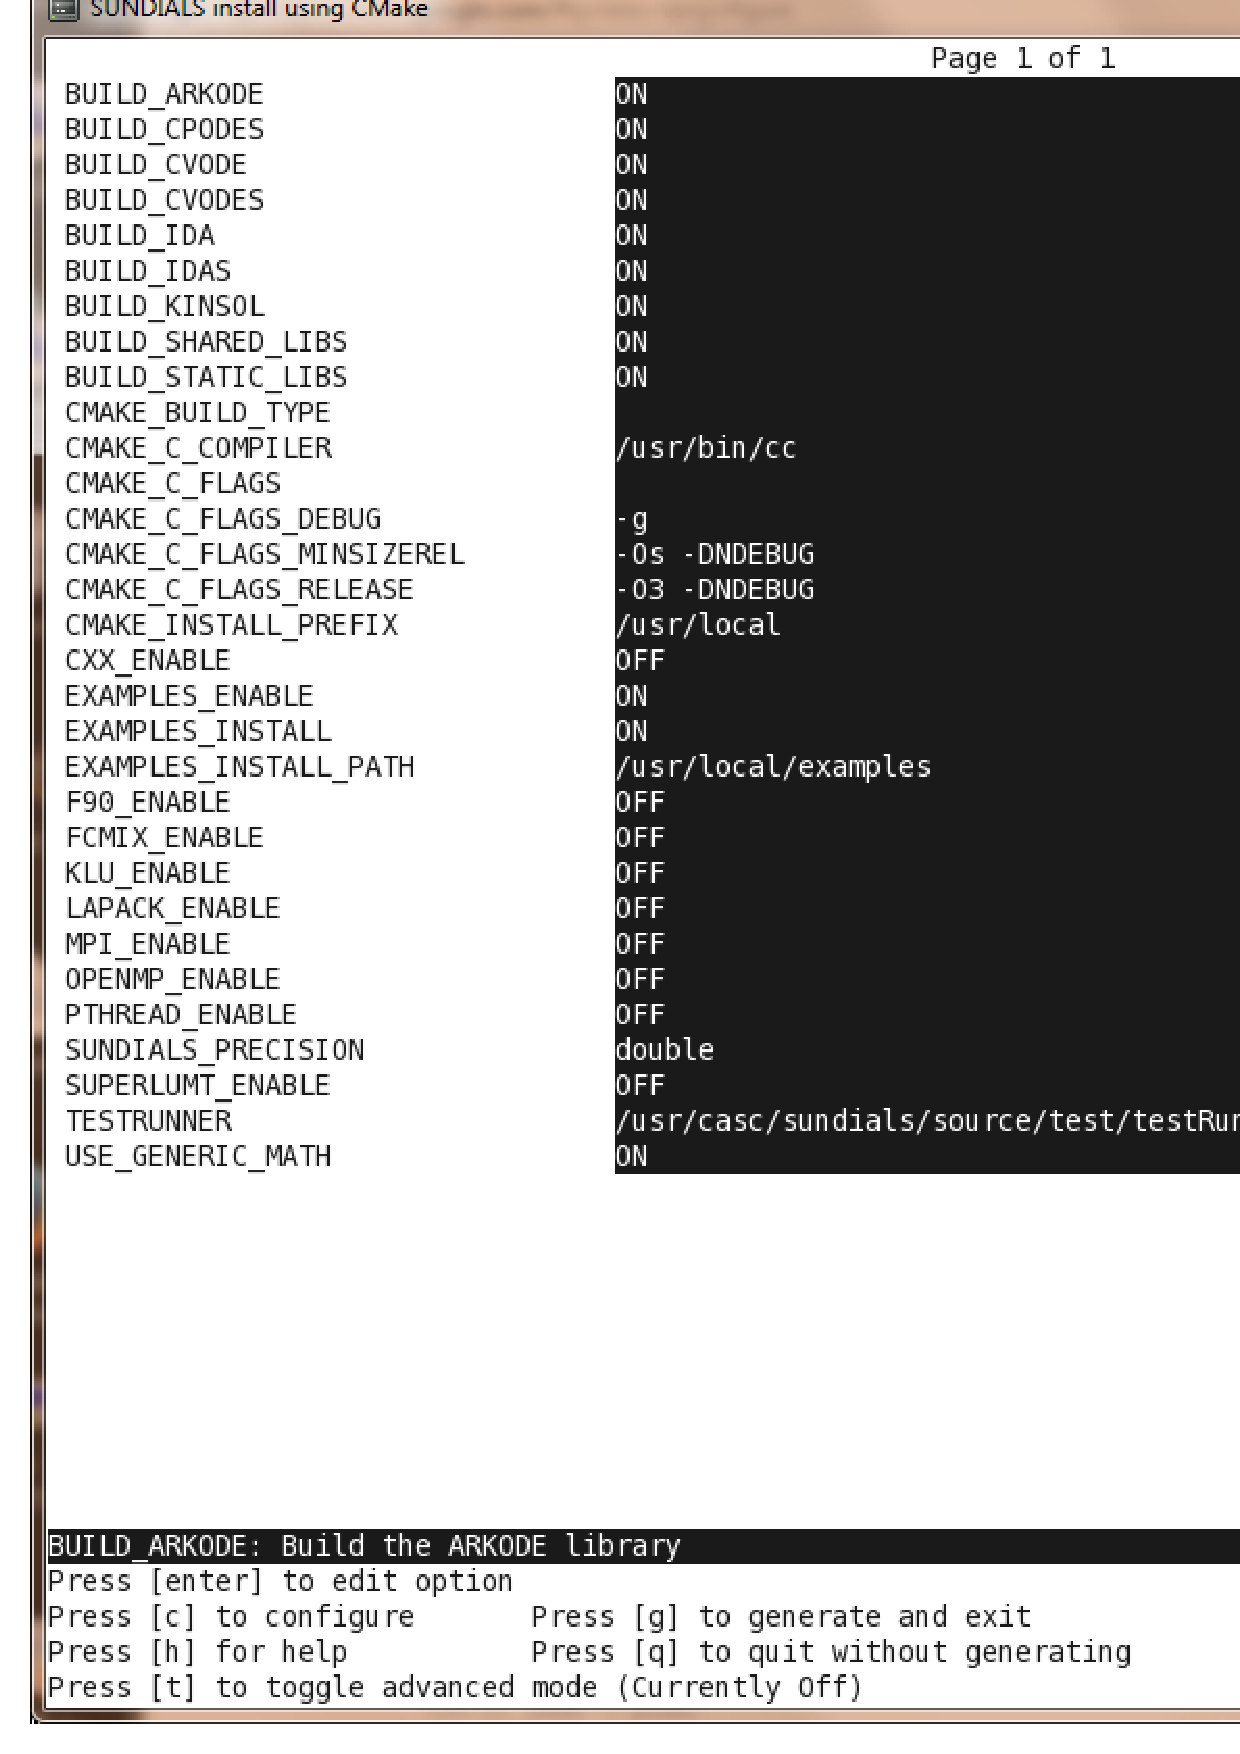
\includegraphics[width=\textwidth]{ccmakedefault}}}
\caption [Initial {\em ccmake} configuration screen]
{Default configuration screen. Note: Initial screen is empty.
To get this default configuration, press 'c' repeatedly (accepting default values denoted with asterisk)
until the 'g' option is available.}
\label{f:ccmakedefault}
\end{figure}

The default {\em instdir} for both {\sundials} and corresponding examples
can be changed by setting the \id{CMAKE\_INSTALL\_PREFIX} and
the \id{EXAMPLES\_INSTALL\_PATH} as shown in figure
\ref{f:ccmakeprefix}. 
\begin{figure}[!ht]
{\centerline{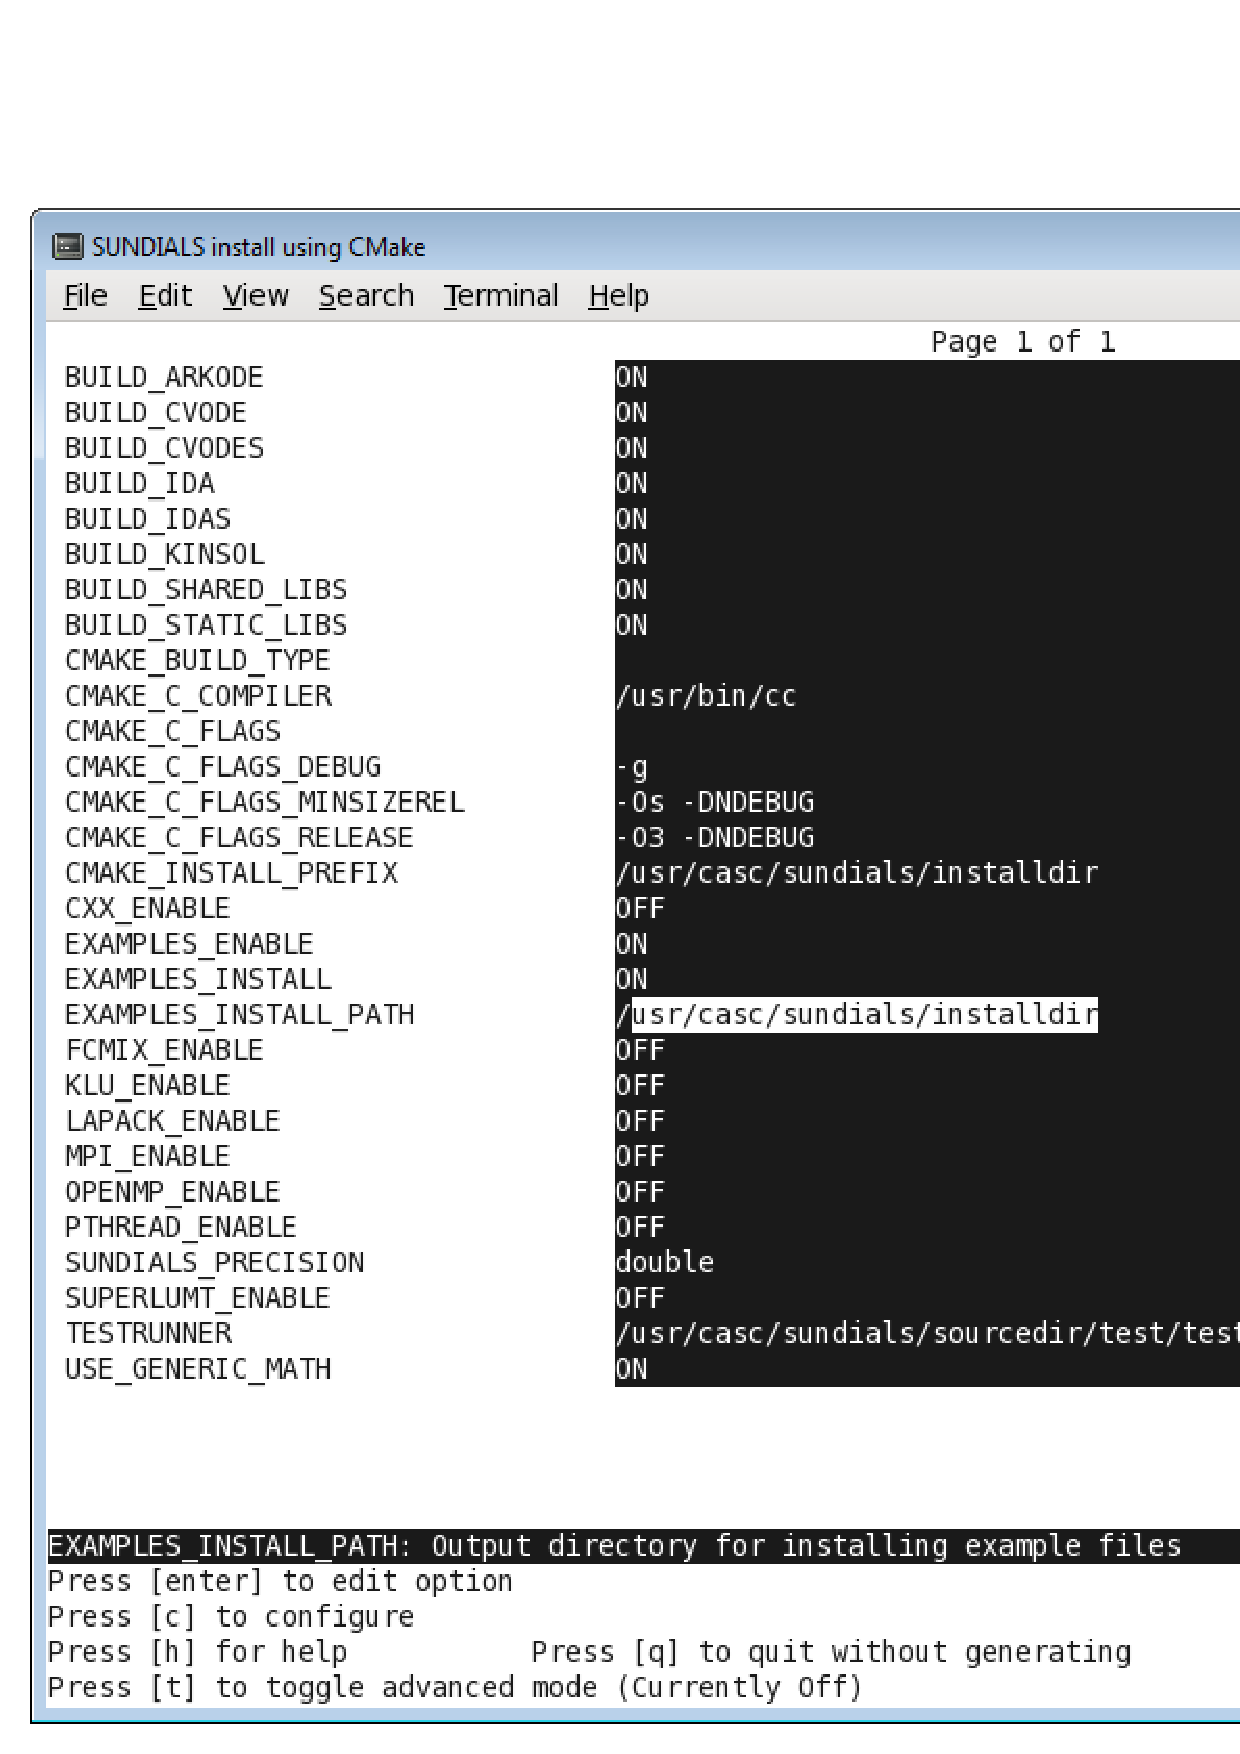
\includegraphics[width=\textwidth]{ccmakeprefix}}}
\caption [Changing the {\em instdir}]
{Changing the {\em instdir} for {\sundials} and
corresponding {\id examples} }
\label{f:ccmakeprefix}
\end{figure}

Pressing the (\id{g} key) will generate makefiles including all dependencies
and all rules to build {\sundials} on this system. 
Back at the command prompt, you can now run:

\begin{verbatim}
  % make
\end{verbatim}

To install {\sundials} in the installation directory specified in the configuration, simply run:

\begin{verbatim}
  % make install
\end{verbatim}

%%
%% *** NOTE: The TestRunner will not be distributed at this time.
%% *** Thus the following is commented out from the documentation.
%% TestRunner
%%
%\subsubsection*{Testing Installation}
%The distribution of {\sundials} includes several examples corresponding to the solvers to be
%installed. Also included in the source bundle is a test script: \id{testRunner}, configured by CMake
%to test the included examples.
%To run the tests, enter:

%\begin{verbatim}
%  % make test
%\end{verbatim}
%The output of \id{testRunner} should look similar to the screens in figure
%\ref{f:testrunner}. The success of each test is based on a line-by-line comparison of expected output files, bundled with the source code, with
%the output of the newly compiled examples. The file compare does allow some differences in rounding for float values.\\\\
%NOTE: Some tests may {\em fail} due to differences in machine architecture, compiler versions, third party libraries etc.{\warn}

%\begin{figure}[!ht]
%{\centerline{\includegraphics{figure=testrunnertop.eps,width=\textwidth}}}
%\vspace{3 mm}
%{\centerline{\includegraphics{figure=testrunnerbot.eps,width=\textwidth}}}
%\caption [Running {\em testRunner}]
%{Invoking {\em testRunner} with {\id make test} to execute all configured
%{\id examples} }
%\label{f:testrunner}
%\end{figure}

 
%%
%% Building from the command line
%%
\subsubsection*{Building from the command line}

Using CMake from the command line is simply a matter of specifying CMake variable settings
with the \id{cmake} command.  The following will build the default configuration:  

\begin{verbatim}
   % cmake -DCMAKE_INSTALL_PREFIX=/home/myname/sundials/instdir \
   > -DEXAMPLES_INSTALL_PATH=/home/myname/sundials/instdir/examples \
   > ../solverdir
   % make
   % make install
\end{verbatim}


\subsection{Configuration options (Unix/Linux)}\label{ss:configuration_options_nix}

A complete list of all available options for a CMake-based {\sundials}
configuration is provide below. Note that the default values shown are for 
a typical configuration on a Linux system and are provided as illustration only.

\begin{description}
\item[\id{BLAS\_ENABLE}] - 
  Enable BLAS support
  \\
  Default: OFF
  \\
  Note: Setting this option to ON will trigger additional CMake
  options. See additional information on building with BLAS enabled
  in \ref{ss:externallibs}.
\item[\id{BLAS\_LIBRARIES}] - 
  BLAS library
  \\
  Default: /usr/lib/libblas.so
  \\
  Note: CMake will search for libraries in your \id{LD\_LIBRARY\_PATH} prior
  to searching default system paths.
\item[\id{BUILD\_ARKODE}] - 
  Build the ARKODE library 
  \\
  Default: ON
\item[\id{BUILD\_CVODE}] - 
  Build the CVODE library 
  \\
  Default: ON
\item[\id{BUILD\_CVODES}] - 
  Build the CVODES library 
  \\
  Default: ON
\item[\id{BUILD\_IDA}] - 
   Build the IDA library 
  \\
   Default: ON
\item[\id{BUILD\_IDAS}] - 
  Build the IDAS library 
  \\
  Default: ON
\item[\id{BUILD\_KINSOL}] - 
  Build the KINSOL library 
  \\
  Default: ON
\item[\id{BUILD\_SHARED\_LIBS}] - 
  Build shared libraries
  \\
  Default: ON
\item[\id{BUILD\_STATIC\_LIBS}] - 
  Build static libraries
  \\
  Default: ON 
\item[\id{CMAKE\_BUILD\_TYPE}] -  
  Choose the type of build, options are: 
  \id{None} (CMAKE\_C\_FLAGS used), \id{Debug}, \id{Release},
  \id{RelWithDebInfo}, and \id{MinSizeRel}
  \\
  Default:
  \\
  Note: Specifying a build type will trigger the corresponding
  build type specific compiler flag options below which will be
  appended to the flags set by
  CMAKE\_{\textless}language{\textgreater}\_FLAGS. 
\item[\id{CMAKE\_C\_COMPILER}] - 
  C compiler
  \\
  Default: /usr/bin/cc 
\item[\id{CMAKE\_C\_FLAGS}] -  
  Flags for C compiler
  \\
  Default:
\item[\id{CMAKE\_C\_FLAGS\_DEBUG}] -      
  Flags used by the C compiler during debug builds
  \\
  Default: -g 
\item[\id{CMAKE\_C\_FLAGS\_MINSIZEREL}] -  
  Flags used by the C compiler during release minsize builds
  \\
  Default: -Os -DNDEBUG 
\item[\id{CMAKE\_C\_FLAGS\_RELEASE}] -    
  Flags used by the C compiler during release builds
  \\
  Default: -O3 -DNDEBUG 
\item[\id{CMAKE\_CXX\_COMPILER}] - 
  {\CPP} compiler
  \\
  Default: /usr/bin/c++
  \\
  Note: A {\CPP} compiler (and all related options) are only
  triggered if {\CPP} examples are enabled (\id{EXAMPLES\_ENABLE\_CXX}
  is ON). All {\sundials} solvers can be used from {\CPP} applications 
  by default without setting any additional configuration options.
\item[\id{CMAKE\_CXX\_FLAGS}] -
  Flags for {\CPP} compiler
  \\
  Default:
\item[\id{CMAKE\_CXX\_FLAGS\_DEBUG}] -
  Flags used by the {\CPP} compiler during debug builds
  \\
  Default: -g 
\item[\id{CMAKE\_CXX\_FLAGS\_MINSIZEREL}] -
  Flags used by the {\CPP} compiler during release minsize builds
  \\
  Default: -Os -DNDEBUG 
\item[\id{CMAKE\_CXX\_FLAGS\_RELEASE}] -
  Flags used by the {\CPP} compiler during release builds
  \\
  Default: -O3 -DNDEBUG
\item[\id{CMAKE\_Fortran\_COMPILER}] - 
  Fortran compiler
  \\
  Default: /usr/bin/gfortran
  \\
  Note: Fortran support (and all related options) are triggered only if
  either Fortran-C support is enabled (\id{FCMIX\_ENABLE} is ON) or
  BLAS/LAPACK support is enabled (\id{BLAS\_ENABLE} or \id{LAPACK\_ENABLE} is ON).
\item[\id{CMAKE\_Fortran\_FLAGS}] - 
  Flags for Fortran compiler
  \\
  Default:
\item[\id{CMAKE\_Fortran\_FLAGS\_DEBUG}] - 
  Flags used by the Fortran compiler during debug builds
  \\
  Default: -g
\item[\id{CMAKE\_Fortran\_FLAGS\_MINSIZEREL}] - 
  Flags used by the Fortran compiler during release minsize builds
  \\
  Default: -Os
\item[\id{CMAKE\_Fortran\_FLAGS\_RELEASE}] - 
  Flags used by the Fortran compiler during release builds
  \\
  Default: -O3
\item[\id{CMAKE\_INSTALL\_PREFIX}] -   
  Install path prefix, prepended onto install directories
  \\
  Default: /usr/local 
  \\
  Note: The user must have write access to the location specified through
  this option. Exported {\sundials} header files and libraries will be 
  installed under subdirectories \id{include} and \id{lib} of 
  \id{CMAKE\_INSTALL\_PREFIX}, respectively.
\item[\id{CUDA\_ENABLE}] -
  Build the {\sundials} {\cuda} vector module.
  \\
  Default: OFF
\item[\id{EXAMPLES\_ENABLE\_C}] -
  Build the {\sundials} {\CC} examples
  \\
  Default: ON
\item[\id{EXAMPLES\_ENABLE\_CUDA}] -
  Build the {\sundials} {\cuda} examples
  \\
  Default: OFF
  \\
  Note: You need to enable {\cuda} support to build these examples.
\item[\id{EXAMPLES\_ENABLE\_CXX}] -
  Build the {\sundials} {\CPP} examples
  \\
  Default: OFF
\item[\id{EXAMPLES\_ENABLE\_RAJA}] -
  Build the {\sundials} {\raja} examples
  \\
  Default: OFF
  \\
  Note: You need to enable {\cuda} and {\raja} support to build these examples.
\item[\id{EXAMPLES\_ENABLE\_F77}] -
  Build the {\sundials} Fortran77 examples
  \\
  Default: ON (if \id{FCMIX\_ENABLE} is ON)
\item[\id{EXAMPLES\_ENABLE\_F90}] -
  Build the {\sundials} Fortran90 examples
  \\
  Default: OFF
\item[\id{EXAMPLES\_INSTALL}] - 
  Install example files
  \\
  Default: ON
  \\
  Note: This option is triggered when any of the {\sundials}
  example programs are enabled \\
  (\id{EXAMPLES\_ENABLE\_$<$language$>$} is ON). If the user requires
  installation of example programs then the sources and sample output files
  for all {\sundials} modules that are currently enabled will be exported to
  the directory specified by \id{EXAMPLES\_INSTALL\_PATH}. A CMake configuration
  script will also be automatically generated and exported to the same directory.
  Additionally, if the configuration is done under a Unix-like system, makefiles
  for the compilation of the example programs (using the installed {\sundials} libraries)
  will be automatically generated and exported to the directory
  specified by \id{EXAMPLES\_INSTALL\_PATH}.
\item[\id{EXAMPLES\_INSTALL\_PATH}] - 
  Output directory for installing example files
  \\
  Default: /usr/local/examples
  \\
  Note: The actual default value for this option will be an \id{examples}
  subdirectory created under \id{CMAKE\_INSTALL\_PREFIX}.
\item[\id{FCMIX\_ENABLE}] - 
  Enable Fortran-C support   
  \\
  Default: OFF 
\item[\id{HYPRE\_ENABLE}] - 
  Enable \textit{hypre} support
  \\
  Default: OFF 
  \\
  Note: See additional information on building with \textit{hypre} enabled in
  \ref{ss:externallibs}. 
\item[\id{HYPRE\_INCLUDE\_DIR}] - 
  Path to \textit{hypre} header files
\item[\id{HYPRE\_LIBRARY\_DIR}] - 
  Path to \textit{hypre} installed library files
\item[\id{KLU\_ENABLE}] - 
  Enable KLU support
  \\
  Default: OFF 
  \\
  Note: See additional information on building with KLU enabled in
  \ref{ss:externallibs}. 
\item[\id{KLU\_INCLUDE\_DIR}] - 
  Path to SuiteSparse header files
\item[\id{KLU\_LIBRARY\_DIR}] - 
  Path to SuiteSparse installed library files
\item[\id{LAPACK\_ENABLE}] -  
  Enable LAPACK support
  \\
  Default: OFF
  \\
  Note: Setting this option to ON will trigger additional CMake
  options. See additional information on building with LAPACK enabled
  in \ref{ss:externallibs}.
\item[\id{LAPACK\_LIBRARIES}] - 
  LAPACK (and BLAS) libraries
  \\
  Default: /usr/lib/liblapack.so;/usr/lib/libblas.so
  \\
  Note: CMake will search for libraries in your \id{LD\_LIBRARY\_PATH} prior
  to searching default system paths.
\item[\id{MPI\_ENABLE}] -
  Enable MPI support (build the parallel nvector).
  \\
  Default: OFF 
  \\
  Note: Setting this option to ON will trigger several additional options
  related to MPI.
\item[\id{MPI\_C\_COMPILER}] -
  \id{mpicc} program
  \\
  Default: 
\item[\id{MPI\_CXX\_COMPILER}] -
  \id{mpicxx} program
  \\
  Default: 
  \\
  Note: This option is triggered only if MPI is enabled
  (\id{MPI\_ENABLE} is ON) and {\CPP} examples are enabled
  (\id{EXAMPLES\_ENABLE\_CXX} is ON). All {\sundials}
  solvers can be used from {\CPP} MPI applications by default
  without setting any additional configuration options other than
  \id{MPI\_ENABLE}.
\item[\id{MPI\_Fortran\_COMPILER}] -
  \id{mpif77} or \id{mpif90} program
  \\
  Default: 
  \\
  Note: This option is triggered only if MPI is enabled
  (\id{MPI\_ENABLE} is ON), Fortran-C support is enabled
  (\id{FCMIX\_ENABLE} is ON), and Fortran77 or Fortran90
  examples are enabled (\id{EXAMPLES\_ENABLE\_F77} or
  \id{EXAMPLES\_ENABLE\_F90} are ON).
\item[\id{MPIEXEC}] -
  Specify the executable for running MPI programs
  \\
  Default: \id{mpirun}
  \\
  Note: This option is triggered only if MPI is enabled
  (\id{MPI\_ENABLE} is ON).
  %% \\
  %% Note: This can either be set to \id{mpirun} for OpenMPI or \id{srun} if jobs are
  %% managed by \id{SLURM} - Simple Linux Utility for Resource Management as exists on
  %% LLNL's high performance computing clusters. 
\item[\id{OPENMP\_ENABLE}] -
  Enable OpenMP support (build the OpenMP nvector).
  \\
  Default: OFF 
\item[\id{PETSC\_ENABLE}] - 
  Enable PETSc support
  \\
  Default: OFF 
  \\
  Note: See additional information on building with PETSc enabled
  in \ref{ss:externallibs}.
\item[\id{PETSC\_INCLUDE\_DIR}] -
  Path to PETSc header files
\item[\id{PETSC\_LIBRARY\_DIR}] - 
  Path to PETSc installed library files
\item[\id{PTHREAD\_ENABLE}] -  
  Enable Pthreads support (build the Pthreads nvector).
  \\
  Default: OFF 
\item[\id{RAJA\_ENABLE}] - 
  Enable {\raja} support (build the {\raja} nvector).
  \\
  Default: OFF 
  \\
  Note: You need to enable {\cuda} in order to build the {\raja} vector module.
\item[\id{SUNDIALS\_F77\_FUNC\_CASE}] - \textbf{advanced option} -
  Specify the case to use in the Fortran name-mangling scheme, options
  are: \id{lower} or \id{upper}
  \\
  Default:
  \\
  Note: The build system will attempt to infer the Fortran
  name-mangling scheme using the Fortran compiler. This option should
  only be used if a Fortran compiler is not available or to override
  the inferred or default (\id{lower}) scheme if one can not be
  determined. If used, \id{SUNDIALS\_F77\_FUNC\_UNDERSCORES} must also
  be set.
\item[\id{SUNDIALS\_F77\_FUNC\_UNDERSCORES}] - \textbf{advanced option} -
  Specify the number of underscores to append in the Fortran
  name-mangling scheme, options are: \id{none}, \id{one}, or \id{two}
  \\
  Default:
  \\
  Note: The build system will attempt to infer the Fortran
  name-mangling scheme using the Fortran compiler. This option should
  only be used if a Fortran compiler is not available or to override
  the inferred or default (\id{one}) scheme if one can not be
  determined. If used, \id{SUNDIALS\_F77\_FUNC\_CASE} must also be set.
\item[\id{SUNDIALS\_INDEX\_TYPE}] - 
  Integer type used for {\sundials} indices, options are: \id{int32\_t} or \id{int64\_t}
  \\
  Default: \id{int64\_t}
\item[\id{SUNDIALS\_PRECISION}] -   
  Precision used in {\sundials}, options are: \id{double}, \id{single}, or \id{extended}
  \\
  Default: \id{double}
\item[\id{SUPERLUMT\_ENABLE}] - 
  Enable SuperLU\_MT support   
  \\
  Default: OFF 
  \\
  Note: See additional information on building with SuperLU\_MT enabled
  in \ref{ss:externallibs}.
\item[\id{SUPERLUMT\_INCLUDE\_DIR}] - 
  Path to SuperLU\_MT header files (typically SRC directory)
\item[\id{SUPERLUMT\_LIBRARY\_DIR}] - 
  Path to SuperLU\_MT installed library files
\item[\id{SUPERLUMT\_THREAD\_TYPE}] - 
  Must be set to Pthread or OpenMP
  \\
  Default: Pthread
\item[\id{USE\_GENERIC\_MATH}] -   
  Use generic (stdc) math libraries
  \\
  Default: ON 
\end{description}

\subsubsection*{xSDK Configuration Options}

{\sundials} supports CMake configuration options defined by the
Extreme-scale Scientific Software Development Kit (xSDK) community
policies (see {\tt https://xsdk.info} for more information). xSDK
CMake options are unused by default but may be activated by setting
\id{USE\_XSDK\_DEFAULTS} to ON.

{\warn} When xSDK options are active, they will overwrite the
corresponding {\sundials} option and may have different default values
(see details below). As such the equivalent {\sundials} options should
not be used when configuring with xSDK options. In the GUI front end
to CMake (\id{ccmake}), setting \id{USE\_XSDK\_DEFAULTS} to ON will
hide the corresponding {\sundials} options as advanced CMake variables.
During configuration, messages are output detailing
which xSDK flags are active and the equivalent {\sundials} options
that are replaced. Below is a complete list xSDK options and the
corresponding {\sundials} options if applicable.

\begin{description}
\item[\id{TPL\_BLAS\_LIBRARIES}] - 
  BLAS library
  \\
  Default: /usr/lib/libblas.so
  \\
  {\sundials} equivalent: \id{BLAS\_LIBRARIES}
  \\
  Note: CMake will search for libraries in your \id{LD\_LIBRARY\_PATH} prior
  to searching default system paths.
\item[\id{TPL\_ENABLE\_BLAS}] - 
  Enable BLAS support
  \\
  Default: OFF
  \\
  {\sundials} equivalent: \id{BLAS\_ENABLE}
\item[\id{TPL\_ENABLE\_HYPRE}] - 
  Enable \textit{hypre} support
  \\
  Default: OFF
  \\
  {\sundials} equivalent: \id{HYPRE\_ENABLE}
\item[\id{TPL\_ENABLE\_KLU}] - 
  Enable KLU support
  \\
  Default: OFF
  \\
  {\sundials} equivalent: \id{KLU\_ENABLE}
\item[\id{TPL\_ENABLE\_PETSC}] - 
  Enable PETSc support
  \\
  Default: OFF
  \\
  {\sundials} equivalent: \id{PETSC\_ENABLE}
\item[\id{TPL\_ENABLE\_LAPACK}] - 
  Enable LAPACK support
  \\
  Default: OFF
  \\
  {\sundials} equivalent: \id{LAPACK\_ENABLE}
\item[\id{TPL\_ENABLE\_SUPERLUMT}] - 
  Enable SuperLU\_MT support
  \\
  Default: OFF
  \\
  {\sundials} equivalent: \id{SUPERLUMT\_ENABLE}
\item[\id{TPL\_HYPRE\_INCLUDE\_DIRS}] - 
  Path to \textit{hypre} header files
  \\
  {\sundials} equivalent: \id{HYPRE\_INCLUDE\_DIR}
\item[\id{TPL\_HYPRE\_LIBRARIES}] - 
  \textit{hypre} library
  \\
  {\sundials} equivalent: N/A
\item[\id{TPL\_KLU\_INCLUDE\_DIRS}] - 
  Path to KLU header files
  \\
  {\sundials} equivalent: \id{KLU\_INCLUDE\_DIR}
\item[\id{TPL\_KLU\_LIBRARIES}] - 
  KLU library
  \\
  {\sundials} equivalent: N/A
\item[\id{TPL\_LAPACK\_LIBRARIES}] - 
  LAPACK (and BLAS) libraries
  \\
  Default: /usr/lib/liblapack.so;/usr/lib/libblas.so
  \\
  {\sundials} equivalent: \id{LAPACK\_LIBRARIES}
  \\
  Note: CMake will search for libraries in your \id{LD\_LIBRARY\_PATH} prior
  to searching default system paths.
\item[\id{TPL\_PETSC\_INCLUDE\_DIRS}] - 
  Path to PETSc header files
  \\
  {\sundials} equivalent: \id{PETSC\_INCLUDE\_DIR}
\item[\id{TPL\_PETSC\_LIBRARIES}] - 
  PETSc library
  \\
  {\sundials} equivalent: N/A
\item[\id{TPL\_SUPERLUMT\_INCLUDE\_DIRS}] - 
  Path to SuperLU\_MT header files
  \\
  {\sundials} equivalent: \id{SUPERLUMT\_INCLUDE\_DIR}
\item[\id{TPL\_SUPERLUMT\_LIBRARIES}] - 
  SuperLU\_MT library
  \\
  {\sundials} equivalent: N/A
\item[\id{TPL\_SUPERLUMT\_THREAD\_TYPE}] - 
  SuperLU\_MT library thread type
  \\
  {\sundials} equivalent: \id{SUPERLUMT\_THREAD\_TYPE}
\item[\id{USE\_XSDK\_DEFAULTS}] - 
  Enable xSDK default configuration settings
  \\
  Default: OFF
  \\
  {\sundials} equivalent: N/A
  \\
  Note: Enabling xSDK defaults also sets \id{CMAKE\_BUILD\_TYPE} to \id{Debug}
\item[\id{XSDK\_ENABLE\_FORTRAN}] -
  Enable {\sundials} Fortran interface
  \\
  Default: OFF
  \\
  {\sundials} equivalent: \id{FCMIX\_ENABLE}
\item[\id{XSDK\_INDEX\_SIZE}] -
  Integer size (bits) used for indices in {\sundials}, options are: \id{32} or \id{64}
  \\
  Default: \id{32}
  \\
  {\sundials} equivalent: \id{SUNDIALS\_INDEX\_TYPE}
\item[\id{XSDK\_PRECISION}] -
  Precision used in {\sundials}, options are: \id{double}, \id{single}, or \id{quad}
  \\
  Default: \id{double}
  \\
  {\sundials} equivalent: \id{SUNDIALS\_PRECISION}
\end{description}



%%===============================================================================

\subsection{Configuration examples}

The following examples will help demonstrate usage of the CMake configure options.

\noindent To configure {\sundials} using the default C and Fortran compilers,
and default \id{mpicc} and \id{mpif77} parallel compilers, 
enable compilation of examples, and install libraries, headers, and
example sources under subdirectories of
\id{/home/myname/sundials/}, use:

\begin{verbatim}
   % cmake \
   > -DCMAKE_INSTALL_PREFIX=/home/myname/sundials/instdir \
   > -DEXAMPLES_INSTALL_PATH=/home/myname/sundials/instdir/examples \
   > -DMPI_ENABLE=ON \
   > -DFCMIX_ENABLE=ON \
   > /home/myname/sundials/solverdir
   %
   % make install
   % 
\end{verbatim}

\noindent To disable installation of the examples, use:
\begin{verbatim}
   % cmake \
   > -DCMAKE_INSTALL_PREFIX=/home/myname/sundials/instdir \
   > -DEXAMPLES_INSTALL_PATH=/home/myname/sundials/instdir/examples \
   > -DMPI_ENABLE=ON \
   > -DFCMIX_ENABLE=ON \
   > -DEXAMPLES_INSTALL=OFF \
   > /home/myname/sundials/solverdir
   %
   % make install
   % 
\end{verbatim}

%%===============================================================================
\subsection{Working with external Libraries} \label{ss:externallibs}

The {\sundials} suite contains many options to enable implementation flexibility
when developing solutions. The following are some notes addressing specific configurations
when using the supported third party libraries.
When building {\sundials} as a shared library external libraries any
used with {\sundials} must also be build as a shared library or as a
static library compiled with the \id{-fPIC} flag.{\warn}

\subsubsection*{Building with BLAS}
{\sundials} does not utilize BLAS directly but it may be needed by other
external libraries that {\sundials} can be built with (e.g. LAPACK,
PETSc, SuperLU\_MT, etc.). To enable BLAS, set the \id{BLAS\_ENABLE}
option to \id{ON}. If the directory containing the BLAS library is in
the \id{LD\_LIBRARY\_PATH} environment variable, CMake will set the
\id{BLAS\_LIBRARIES} variable accordingly, otherwise CMake will
attempt to find the BLAS library in standard system locations. To
explicitly tell CMake what libraries to use, the \id{BLAS\_LIBRARIES}
variable can be set to the desired library. Example:
\begin{verbatim}
   % cmake \
   > -DCMAKE_INSTALL_PREFIX=/home/myname/sundials/instdir \
   > -DEXAMPLES_INSTALL_PATH=/home/myname/sundials/instdir/examples \
   > -DBLAS_ENABLE=ON \
   > -DBLAS_LIBRARIES=/myblaspath/lib/libblas.so \
   > -DSUPERLUMT_ENABLE=ON \
   > -DSUPERLUMT_INCLUDE_DIR=/mysuperlumtpath/SRC
   > -DSUPERLUMT_LIBRARY_DIR=/mysuperlumtpath/lib
   > /home/myname/sundials/solverdir
   %
   % make install
   % 
\end{verbatim}
{\warn}When allowing CMake to automatically locate the LAPACK library,
CMake \textit{may} also locate the corresponding BLAS library.

If a working Fortran compiler is not available to infer the Fortran
name-mangling scheme, the options \id{SUNDIALS\_F77\_FUNC\_CASE} and
\id{SUNDIALS\_F77\_FUNC\_UNDERSCORES} \textit{must} be set in order to
bypass the check for a Fortran compiler and define the name-mangling
scheme. The defaults for these options in earlier versions of
{\sundials} were \id{lower} and \id{one} respectively.


\subsubsection*{Building with LAPACK}
To enable LAPACK, set the \id{LAPACK\_ENABLE} option to \id{ON}.
If the directory containing the LAPACK library is in the
\id{LD\_LIBRARY\_PATH} environment variable, CMake will set the
\id{LAPACK\_LIBRARIES} variable accordingly, otherwise CMake will
attempt to find the LAPACK library in standard system locations. To
explicitly tell CMake what library to use, the \id{LAPACK\_LIBRARIES}
variable can be set to the desired libraries. {\warn}When setting
the LAPACK location explicitly the location of the corresponding BLAS
library will also need to be set. Example:
\begin{verbatim}
   % cmake \
   > -DCMAKE_INSTALL_PREFIX=/home/myname/sundials/instdir \
   > -DEXAMPLES_INSTALL_PATH=/home/myname/sundials/instdir/examples \
   > -DBLAS_ENABLE=ON \
   > -DBLAS_LIBRARIES=/mylapackpath/lib/libblas.so \
   > -DLAPACK_ENABLE=ON \
   > -DLAPACK_LIBRARIES=/mylapackpath/lib/liblapack.so \
   > /home/myname/sundials/solverdir
   %
   % make install
   % 
\end{verbatim}
{\warn}When allowing CMake to automatically locate the LAPACK library,
CMake \textit{may} also locate the corresponding BLAS library.

If a working Fortran compiler is not available to infer the Fortran
name-mangling scheme, the options \id{SUNDIALS\_F77\_FUNC\_CASE} and
\id{SUNDIALS\_F77\_FUNC\_UNDERSCORES} \textit{must} be set in order to
bypass the check for a Fortran compiler and define the name-mangling
scheme. The defaults for these options in earlier versions of
{\sundials} were \id{lower} and \id{one} respectively.

\subsubsection*{Building with KLU}
The KLU libraries are part of SuiteSparse, a suite of sparse matrix software,
available from the Texas A\&M University website: {\tt http://faculty.cse.tamu.edu/davis/suitesparse.html}.
{\sundials} has been tested with SuiteSparse version 4.5.3.
To enable KLU, set \id{KLU\_ENABLE} to \id{ON}, set \id{KLU\_INCLUDE\_DIR} to the \id{include}
path of the KLU installation and set \id{KLU\_LIBRARY\_DIR} to the \id{lib} path of the KLU installation.
The CMake configure will result in populating the following variables: \id{AMD\_LIBRARY},
\id{AMD\_LIBRARY\_DIR}, \id{BTF\_LIBRARY}, \id{BTF\_LIBRARY\_DIR},
\id{COLAMD\_LIBRARY}, \id{COLAMD\_LIBRARY\_DIR}, and
\newline\id{KLU\_LIBRARY}.

\subsubsection*{Building with SuperLU\_MT}
The SuperLU\_MT libraries are available for download from the Lawrence Berkeley National Laboratory website:
{\tt http://crd-legacy.lbl.gov/$\sim$xiaoye/SuperLU/\#superlu\_mt}. 
{\sundials} has been tested with SuperLU\_MT version 3.1. 
To enable SuperLU\_MT, set  \id{SUPERLUMT\_ENABLE} to \id{ON}, set \id{SUPERLUMT\_INCLUDE\_DIR}
to the \id{SRC} path of the SuperLU\_MT installation, and set the variable
\newline\id{SUPERLUMT\_LIBRARY\_DIR} to the \id{lib} path of the SuperLU\_MT installation.
At the same time, the variable
\id{SUPERLUMT\_THREAD\_TYPE} must be set to either \id{Pthread} or \id{OpenMP}.

\noindent Do not mix thread types when building {\sundials} solvers.
If threading is enabled for {\sundials} by having either \id{OPENMP\_ENABLE} or \id{PTHREAD\_ENABLE} set to \id{ON}
then SuperLU\_MT should be set to use the same threading type.{\warn}

\subsubsection*{Building with PETSc}
The PETSc libraries are available for download from the Argonne National Laboratory website:
{\tt http://www.mcs.anl.gov/petsc}. 
{\sundials} has been tested with PETSc version 3.7.2. 
To enable PETSc, set  \id{PETSC\_ENABLE} to \id{ON}, set \id{PETSC\_INCLUDE\_DIR}
to the \id{include} path of the PETSc installation, and set the variable
\id{PETSC\_LIBRARY\_DIR} to the \id{lib} path of the PETSc installation.


\subsubsection*{Building with \textit{hypre}}
The \textit{hypre} libraries are available for download from the Lawrence Livermore
National Laboratory website: {\tt http://computation.llnl.gov/projects/hypre}.
%{\tt http://computation.llnl.gov/projects/hypre-scalable-linear-solvers-multigrid-methods}.
{\sundials} has been tested with \textit{hypre} version 2.11.1. 
To enable \textit{hypre}, set  \id{HYPRE\_ENABLE} to \id{ON}, set \id{HYPRE\_INCLUDE\_DIR}
to the \id{include} path of the \textit{hypre} installation, and set the variable
\id{HYPRE\_LIBRARY\_DIR} to the \id{lib} path of the \textit{hypre} installation.

\subsubsection*{Building with CUDA}
{\sundials} {\cuda} modules and examples have been tested with version 8.0 of the 
{\cuda} toolkit. To build them, you need to install the Toolkit and compatible
NVIDIA drivers. Both are available for download from the NVIDIA website:
{\tt https://developer.nvidia.com/cuda-downloads}. To enable {\cuda}, 
set \id{CUDA\_ENABLE} to \id{ON}. If {\cuda} is installed in a
nonstandard location, you may be prompted to set the variable
\id{CUDA\_TOOLKIT\_ROOT\_DIR} with your {\cuda} Toolkit installation
path. To enable {\cuda} examples, set \id{EXAMPLES\_ENABLE\_CUDA} to \id{ON}.

\subsubsection*{Building with RAJA}
{\raja} is a performance portability layer developed by Lawrence
Livermore National Laboratory and can be obtained from {\tt https://github.com/LLNL/RAJA}.
{\sundials} {\raja} modules and examples have been tested with {\raja}
version 0.3. Building {\sundials} {\raja} modules requires a
{\cuda}-enabled {\raja} installation. To enable {\raja}, set
\id{CUDA\_ENABLE} and \id{RAJA\_ENABLE} to \id{ON}. If {\raja} is
installed in a nonstandard location you will be prompted to set the
variable \id{RAJA\_DIR} with the path to the {\raja} CMake
configuration file. To enable building the {\raja} examples set
\id{EXAMPLES\_ENABLE\_RAJA} to \id{ON}.

\subsection{Testing the build and installation}

If {\sundials} was configured with
\id{EXAMPLES\_ENABLE\_$<$language$>$} options to \id{ON}, then a set of
regression tests can be run after building with the \id{make} command
by running: 
\begin{verbatim}
  % make test
\end{verbatim}
Additionally, if \id{EXAMPLES\_INSTALL} was also set to \id{ON}, then
a set of smoke tests can be run after installing with the \id{make install} 
command by running:
\begin{verbatim}
  % make test_install
\end{verbatim}

%%===============================================================================
\section{Building and Running Examples}
%%===============================================================================
Each of the {\sundials} solvers is distributed with a set of examples
demonstrating basic usage. To build and install the examples, set at
least of the \id{EXAMPLES\_ENABLE\_$<$language$>$} options to \id{ON}, and
set \id{EXAMPLES\_INSTALL} to \id{ON}.
Specify the installation path for the examples with the variable \id{EXAMPLES\_INSTALL\_PATH}. CMake will generate
\id{CMakeLists.txt} configuration files (and \id{Makefile} files if on Linux/Unix) that reference the
{\em installed} {\sundials} headers and libraries.

Either the \id{CMakeLists.txt} file or the traditional \id{Makefile} may be used to build the examples
as well as serve as a template for creating user developed solutions.
To use the supplied \id{Makefile} simply run \id{make} to compile and generate the executables.
To use CMake from within the installed example directory, run \id{cmake} (or \id{ccmake} to use the GUI)
followed by \id{make} to compile the example code.
Note that if CMake is used, it will overwrite the traditional \id{Makefile} with a new CMake-generated \id{Makefile}.
The resulting output from running the examples can be compared with example output bundled
in the {\sundials} distribution.

\noindent NOTE: There will potentially be differences in the output due to machine architecture, compiler versions,
use of third party libraries etc.{\warn} 


%%===============================================================================
\section{Configuring, building, and installing  on Windows}\label{s:cmake_windows}
%%===============================================================================
CMake can also be used to build {\sundials} on Windows. To build {\sundials} for
use with Visual Studio the following steps should be performed:
\begin{enumerate}
\item Unzip the downloaded tar file(s) into a directory. This will be the {\em solverdir} 
\item Create a separate {\em builddir}
\item Open a Visual Studio Command Prompt and cd to {\em builddir}
\item Run cmake-gui ../{\em solverdir}
\begin{enumerate}
\item Hit Configure
\item Check/Uncheck solvers to be built
\item Change CMAKE\_INSTALL\_PREFIX to {\em instdir}
\item Set other options as desired
\item Hit Generate
\end{enumerate}
\item Back in the VS Command Window:
\begin{enumerate}
\item Run msbuild ALL\_BUILD.vcxproj
\item Run msbuild INSTALL.vcxproj
\end{enumerate} 
\end{enumerate}

\noindent The resulting libraries will be in the {\em instdir}.
\noindent The {\sundials} project can also now be opened in Visual Studio.
Double click on the ALL\_BUILD.vcxproj file to open the project.
Build the whole {\em solution} to create the {\sundials} libraries.
To use the {\sundials} libraries in your own projects, you must
set the include directories for your project,
add the {\sundials} libraries to your project solution,
and set the {\sundials} libraries as dependencies for your project.

%%===============================================================================
\section{Installed libraries and exported header files}
%%===============================================================================

Using the CMake {\sundials} build system, the command
\begin{verbatim}
   % make install
\end{verbatim}
will install the libraries under {\em libdir} and the public header
files under {\em includedir}. The values for these directories are
{\em instdir}\id{/lib} and {\em instdir}\id{/include},
respectively. The location can be changed by setting the CMake variable \id{CMAKE\_INSTALL\_PREFIX}.
Although all installed libraries reside under {\em libdir}\id{/lib}, the public header files
are further organized into subdirectories under {\em includedir}\id{/include}.

The installed libraries and exported header files are listed for
reference in Table \ref{t:sundials_files}.
The file extension .{\em lib}
is typically \id{.so} for shared libraries and \id{.a} for static libraries.
Note that, in the Tables, names are relative to {\em libdir}
for libraries and to {\em includedir} for header files.

A typical user program need not explicitly include any of the shared
{\sundials} header files from under the {\em includedir}\id{/include}\id{/sundials}
directory since they are explicitly included by the appropriate solver
header files ({\em e.g.}, \id{cvode\_dense.h} includes
\id{sundials\_dense.h}). However, it is both legal and safe to do so,
and would be useful, for example, if the functions declared in \id{sundials\_dense.h} 
are to be used in building a preconditioner.

%---------------------------------------------------------------------------
% Table of installed files
%---------------------------------------------------------------------------

\newlength{\colLenOne}
\settowidth{\colLenOne}{{\sunlinsollapdense}}

\newlength{\colLenTwo}
\settowidth{\colLenTwo}{Header files}

\newlength{\colLenThree}
\setlength{\colLenThree}{\textwidth}
\addtolength{\colLenThree}{-0.5in}
\addtolength{\colLenThree}{-\colLenOne}
\addtolength{\colLenThree}{-\colLenTwo}

%\caption{{\sundials} libraries and header files (cont.)}\label{t:sundials_files2}

\tablecaption{{\sundials} libraries and header files}\label{t:sundials_files}
\tablefirsthead{\hline}
\tablehead{\hline \multicolumn{4}{|l|}{\small\slshape continued from last page} \\
           \hline}
\tabletail{\hline \multicolumn{4}{|r|}{\small\slshape continued on next page} \\ \hline}
\begin{xtabular}{|p{\colLenOne}|p{\colLenTwo}|p{0.5\colLenThree} p{0.5\colLenThree}|}

%% --------------------------------------------------
{\shared}
 & Libraries    & n/a  & \\
\cline{2-4}
 & Header files & sundials/sundials\_config.h        & sundials/sundials\_fconfig.h  \\
 &              & sundials/sundials\_types.h         & sundials/sundials\_math.h     \\
 &              & sundials/sundials\_nvector.h       & sundials/sundials\_fnvector.h \\
 &              & sundials/sundials\_iterative.h     & sundials/sundials\_direct.h   \\
 &              & sundials/sundials\_dense.h         & sundials/sundials\_band.h     \\
 &              & sundials/sundials\_matrix.h        & sundials/sundials\_version.h  \\
 &              & sundials/sundials\_linearsolver.h  & \\
\hline
%% --------------------------------------------------
{\nvecs}
 & Libraries    & libsundials\_nvecserial.{\em lib} & libsundials\_fnvecserial.a \\ 
\cline{2-4}
 & Header files & nvector/nvector\_serial.h         & \\ 
\hline
%% --------------------------------------------------
{\nvecp}
 & Libraries    & libsundials\_nvecparallel.{\em lib} & libsundials\_fnvecparallel.a \\
\cline{2-4}
 & Header files & nvector/nvector\_parallel.h         & \\
\hline
%% --------------------------------------------------
{\nvecopenmp}
 & Libraries    & libsundials\_nvecopenmp.{\em lib} & libsundials\_fnvecopenmp.a \\ 
\cline{2-4}
 & Header files & nvector/nvector\_openmp.h         & \\ 
\hline
%% --------------------------------------------------
{\nvecpthreads}
 & Libraries    & libsundials\_nvecpthreads.{\em lib} & libsundials\_fnvecpthreads.a \\ 
\cline{2-4}
 & Header files & nvector/nvector\_pthreads.h         & \\ 
\hline
%% --------------------------------------------------
{\nvecph}
 & Libraries    & libsundials\_nvecparhyp.{\em lib} & \\
\cline{2-4}
 & Header files & nvector/nvector\_parhyp.h         & \\ 
\hline
%% --------------------------------------------------
{\nvecpetsc}
 & Libraries    & libsundials\_nvecpetsc.{\em lib} & \\ 
\cline{2-4}
 & Header files & nvector/nvector\_petsc.h         & \\ 
\hline
%% --------------------------------------------------
{\nveccuda}
 & Libraries    & libsundials\_nveccuda.{\em lib}     & \\ 
\cline{2-4}
 & Header files & nvector/nvector\_cuda.h             & \\
 &              & nvector/cuda/ThreadPartitioning.hpp & \\
 &              & nvector/cuda/Vector.hpp             & \\
 &              & nvector/cuda/VectorKernels.cuh      & \\
\hline
%% --------------------------------------------------
{\nvecraja}
 & Libraries    & libsundials\_nvecraja.{\em lib} & \\ 
\cline{2-4}
 & Header files & nvector/nvector\_raja.h         & \\
 &              & nvector/raja/Vector.hpp         & \\
\hline
%% --------------------------------------------------
{\sunmatband}
 & Libraries    & libsundials\_sunmatrixband.{\em lib} & \\ 
 &              & libsundials\_fsunmatrixband.a        & \\ 
\cline{2-4}
 & Header files & sunmatrix/sunmatrix\_band.h          & \\ 
\hline
%% --------------------------------------------------
{\sunmatdense}
 & Libraries    & libsundials\_sunmatrixdense.{\em lib} & \\
 &              & libsundials\_fsunmatrixdense.a        & \\
\cline{2-4}
 & Header files & sunmatrix/sunmatrix\_dense.h          & \\
\hline
%% --------------------------------------------------
{\sunmatsparse}
 & Libraries    & libsundials\_sunmatrixsparse.{\em lib} & \\ 
 &              & libsundials\_fsunmatrixsparse.a        & \\ 
\cline{2-4}
 & Header files & sunmatrix/sunmatrix\_sparse.h          & \\ 
\hline
%% --------------------------------------------------
{\sunlinsolband}
 & Libraries    & libsundials\_sunlinsolband.{\em lib} & \\ 
 &              & libsundials\_fsunlinsolband.a        & \\ 
\cline{2-4}
 & Header files & sunlinsol/sunlinsol\_band.h          & \\ 
\hline
%% --------------------------------------------------
{\sunlinsoldense}
 & Libraries    & libsundials\_sunlinsoldense.{\em lib} & \\ 
 &              & libsundials\_fsunlinsoldense.a        & \\ 
\cline{2-4}
 & Header files & sunlinsol/sunlinsol\_dense.h          & \\ 
\hline
%% --------------------------------------------------
{\sunlinsolklu}
 & Libraries    & libsundials\_sunlinsolklu.{\em lib} & \\ 
 &              & libsundials\_fsunlinsolklu.a        & \\ 
\cline{2-4}
 & Header files & sunlinsol/sunlinsol\_klu.h          & \\ 
\hline
%% --------------------------------------------------
{\sunlinsollapband}
 & Libraries    & libsundials\_sunlinsollapackband.{\em lib} & \\ 
 &              & libsundials\_fsunlinsollapackband.a        & \\ 
\cline{2-4}
 & Header files & sunlinsol/sunlinsol\_lapackband.h          & \\ 
\hline
%% --------------------------------------------------
{\sunlinsollapdense}
 & Libraries    & libsundials\_sunlinsollapackdense.{\em lib} & \\ 
 &              & libsundials\_fsunlinsollapackdense.a        & \\ 
\cline{2-4}
 & Header files & sunlinsol/sunlinsol\_lapackdense.h          & \\ 
\hline
%% --------------------------------------------------
{\sunlinsolpcg}
 & Libraries    & libsundials\_sunlinsolpcg.{\em lib} & \\ 
 &              & libsundials\_fsunlinsolpcg.a        & \\ 
\cline{2-4}
 & Header files & sunlinsol/sunlinsol\_pcg.h          & \\ 
\hline
%% --------------------------------------------------
{\sunlinsolspbcgs}
 & Libraries    & libsundials\_sunlinsolspbcgs.{\em lib} & \\ 
 &              & libsundials\_fsunlinsolspbcgs.a        & \\ 
\cline{2-4}
 & Header files & sunlinsol/sunlinsol\_spbcgs.h          & \\ 
\hline
%% --------------------------------------------------
{\sunlinsolspfgmr}
 & Libraries    & libsundials\_sunlinsolspfgmr.{\em lib} & \\ 
 &              & libsundials\_fsunlinsolspfgmr.a        & \\ 
\cline{2-4}
 & Header files & sunlinsol/sunlinsol\_spfgmr.h          & \\ 
\hline
%% --------------------------------------------------
{\sunlinsolspgmr}
 & Libraries    & libsundials\_sunlinsolspgmr.{\em lib} & \\ 
 &              & libsundials\_fsunlinsolspgmr.a        & \\ 
\cline{2-4}
 & Header files & sunlinsol/sunlinsol\_spgmr.h          & \\ 
\hline
%% --------------------------------------------------
{\sunlinsolsptfqmr}
 & Libraries    & libsundials\_sunlinsolsptfqmr.{\em lib} & \\ 
 &              & libsundials\_fsunlinsolsptfqmr.a        & \\ 
\cline{2-4}
 & Header files & sunlinsol/sunlinsol\_sptfqmr.h          & \\ 
\hline
%% --------------------------------------------------
{\sunlinsolslumt}
 & Libraries    & libsundials\_sunlinsolsuperlumt.{\em lib} & \\ 
 &              & libsundials\_fsunlinsolsuperlumt.a        & \\ 
\cline{2-4}
 & Header files & sunlinsol/sunlinsol\_superlumt.h          & \\ 
\hline
%% --------------------------------------------------
{\cvode}
 & Libraries    & libsundials\_cvode.{\em lib} & libsundials\_fcvode.a \\
\cline{2-4}
 & Header files & cvode/cvode.h                & cvode/cvode\_impl.h   \\
 &              & cvode/cvode\_direct.h        & cvode/cvode\_spils.h  \\
 &              & cvode/cvode\_bandpre.h       & cvode/cvode\_bbdpre.h \\
\hline
%% --------------------------------------------------
{\cvodes}
 & Libraries    & libsundials\_cvodes.{\em lib} & \\
\cline{2-4}
 & Header files & cvodes/cvodes.h               & cvodes/cvodes\_impl.h   \\
 &              & cvodes/cvodes\_direct.h       & cvodes/cvodes\_spils.h  \\
 &              & cvodes/cvodes\_bandpre.h      & cvodes/cvodes\_bbdpre.h \\
\hline
%% --------------------------------------------------
{\arkode}
 & Libraries    & libsundials\_arkode.{\em lib} & libsundials\_farkode.a \\
\cline{2-4}
 & Header files & arkode/arkode.h               & arkode/arkode\_impl.h   \\
 &              & arkode/arkode\_direct.h       & arkode/arkode\_spils.h  \\
 &              & arkode/arkode\_bandpre.h      & arkode/arkode\_bbdpre.h \\
\hline
%% --------------------------------------------------
{\ida}
 & Libraries    & libsundials\_ida.{\em lib} & libsundials\_fida.a \\
\cline{2-4}
 & Header files & ida/ida.h                  & ida/ida\_impl.h     \\
 &              & ida/ida\_direct.h          & ida/ida\_spils.h    \\
 &              & ida/ida\_bbdpre.h          & \\
\hline
%% --------------------------------------------------
{\idas}
 & Libraries    & libsundials\_idas.{\em lib} & \\
\cline{2-4}
 & Header files & idas/idas.h                 & idas/idas\_impl.h     \\
 &              & idas/idas\_direct.h         & idas/idas\_spils.h    \\
 &              & idas/idas\_bbdpre.h         & \\
\hline 
%% --------------------------------------------------
{\kinsol}
 & Libraries    & libsundials\_kinsol.{\em lib} & libsundials\_fkinsol.a \\
\cline{2-4}
 & Header files & kinsol/kinsol.h               & kinsol/kinsol\_impl.h     \\
 &              & kinsol/kinsol\_direct.h       & kinsol/kinsol\_spils.h    \\
 &              & kinsol/kinsol\_bbdpre.h       & \\
\hline
 %% --------------------------------------------------
\end{xtabular}

\clearemptydoublepage
%===============================================================
% IDA constants
%%========================================================================
\chapter{IDA Constants}\label{c:constants}
%%========================================================================

Below we list all input and output constants used by the main solver and 
linear solver modules, together with their numerical values and a short
description of their meaning.

%%-------------------------------------------------------------------------
%% Supertabular setings

\newlength{\tcolone}
\settowidth{\tcolone}{\id{SPTFQMR\_PSOLVE\_FAIL\_UNREC}}
\newlength{\tcoltwo}
\settowidth{\tcoltwo}{-20}
\newlength{\tcolthree}
\setlength{\tcolthree}{\textwidth}
\addtolength{\tcolthree}{-0.5in}
\addtolength{\tcolthree}{-\tcolone}
\addtolength{\tcolthree}{-\tcoltwo}

\tablefirsthead{}
\tablehead{}
\tabletail{}
\tablelasttail{}

%%-------------------------------------------------------------------------

\section{IDA input constants}\label{s:ida_in_constants}

\begin{xtabular*}{\textwidth}{p{\tcolone}@{\hspace*{2mm}\extracolsep{\fill}}rp{\tcolthree}}

\hline
\multicolumn{3}{c}{\bf {\ida} main solver module}\\
\hline\\

\id{IDA\_NORMAL}           & 1 & Solver returns at specified output time. \\
\id{IDA\_ONE\_STEP}        & 2 & Solver returns after each successful step. \\
\id{IDA\_YA\_YDP\_INIT}    & 1 & Compute $y_a$ and $\dot{y}_d$, given $y_d$.\\
\id{IDA\_Y\_INIT}          & 2 & Compute $y$, given $\dot{y}$.\\


\\\hline
\multicolumn{3}{c}{\bf Iterative linear solver module}\\
\hline\\

\id{PREC\_NONE}  &  0 & No preconditioning \\
\id{PREC\_LEFT}  &  1 & Preconditioning on the left. \\
\id{MODIFIED\_GS}  & 1 & Use modified Gram-Schmidt procedure. \\
\id{CLASSICAL\_GS} & 2 & Use classical Gram-Schmidt procedure. \\

\end{xtabular*}

%%-------------------------------------------------------------------------

\section{IDA output constants}\label{s:ida_out_constants}

\begin{xtabular*}{\textwidth}{p{\tcolone}@{\hspace*{2mm}\extracolsep{\fill}}rp{\tcolthree}}

\hline
\multicolumn{3}{c}{\bf {\ida} main solver module}\\
\hline\\
\id{IDA\_SUCCESS}         &  0  & Successful function return. \\
\id{IDA\_TSTOP\_RETURN}   &  1  & \id{IDASolve} succeeded by reaching the specified stopping point. \\
\id{IDA\_ROOT\_RETURN}    &  2  & \id{IDASolve} succeeded and found one or more roots. \\
\id{IDA\_WARNING}         & 99  & \id{IDASolve} succeeded but an unusual situation occurred. \\
\id{IDA\_TOO\_MUCH\_WORK} & -1  & The solver took \id{mxstep} internal steps but could not reach tout.\\
\id{IDA\_TOO\_MUCH\_ACC}  & -2  & The solver could not satisfy the accuracy demanded by the user for some internal step.\\
\id{IDA\_ERR\_FAIL}       & -3  & Error test failures occurred too many times during one internal time step or minimum step size was reached. \\
\id{IDA\_CONV\_FAIL}      & -4  & Convergence test failures occurred too many times during one internal time step or minimum step size was reached. \\
\id{IDA\_LINIT\_FAIL}     & -5  & The linear solver's initialization function failed.  \\
\id{IDA\_LSETUP\_FAIL}    & -6  & The linear solver's setup function failed in an unrecoverable manner. \\
\id{IDA\_LSOLVE\_FAIL}    & -7  & The linear solver's solve function failed in an unrecoverable manner. \\
\id{IDA\_RES\_FAIL}       & -8  & The user-provided residual function failed in an unrecoverable manner. \\
\id{IDA\_REP\_RES\_FAIL}  & -9  & The user-provided residual function repeatedly returned a recoverable error flag, but the solver was unable to recover. \\
\id{IDA\_RTFUNC\_FAIL}    & -10 & The rootfinding function failed in an unrecoverable manner. \\
\id{IDA\_CONSTR\_FAIL}    & -11 & The inequality constraints were violated and the solver was unable to recover. \\
\id{IDA\_FIRST\_RES\_FAIL}& -12 & The user-provided residual function failed recoverably on the first call. \\
\id{IDA\_LINESEARCH\_FAIL}& -13 & The line search failed. \\
\id{IDA\_NO\_RECOVERY}    & -14 & The residual function, linear solver setup function, or linear solver solve function had a recoverable failure, but \id{IDACalcIC} could not recover. \\
\id{IDA\_MEM\_NULL}       & -20  & The \id{ida\_mem} argument was \id{NULL}. \\
\id{IDA\_MEM\_FAIL}       & -21 & A memory allocation failed. \\
\id{IDA\_ILL\_INPUT}      & -22 & One of the function inputs is illegal. \\
\id{IDA\_NO\_MALLOC}      & -23 & The {\ida} memory was not allocated by a call to \id{IDAInit}. \\
\id{IDA\_BAD\_EWT}        & -24 & Zero value of some error weight component. \\
\id{IDA\_BAD\_K}          & -25 & The $k$-th derivative is not available. \\
\id{IDA\_BAD\_T}          & -26 & The time $t$ is outside the last step taken. \\
\id{IDA\_BAD\_DKY}        & -27 & The vector argument where derivative should be stored is \id{NULL}. \\

\\\hline
\multicolumn{3}{c}{\bf {\idadls} linear solver modules}\\
\hline\\

%% CSW: We should make these generic to the solver and not have error labels specific to the integrators.
\id{IDADLS\_SUCCESS}    &  0 & Successful function return. \\
\id{IDADLS\_MEM\_NULL}  & -1 & The \id{ida\_mem} argument was \id{NULL}.\\
\id{IDADLS\_LMEM\_NULL} & -2 & The {\idadls} linear solver has not been initialized.\\
\id{IDADLS\_ILL\_INPUT} & -3 & The {\idadls} solver is not compatible with the current {\nvector} module.\\
\id{IDADLS\_MEM\_FAIL}  & -4 & A memory allocation request failed.\\
\id{IDADLS\_JACFUNC\_UNRECVR} & -5 & The Jacobian function failed in an unrecoverable manner. \\
\id{IDADLS\_JACFUNC\_RECVR}   & -6 & The Jacobian function had a recoverable error. \\
\id{IDADLS\_SUNMAT\_FAIL}     & -7 & An error occurred with the current {\sunmatrix} module. \\

%% \\\hline
%% \multicolumn{3}{c}{\bf {\idasls} linear solver module}\\
%% \hline\\

%% \id{IDASLS\_SUCCESS}    &  0 & Successful function return. \\
%% \id{IDASLS\_MEM\_NULL}  & -1 & The \id{ida\_mem} argument was \id{NULL}.\\
%% \id{IDASLS\_LMEM\_NULL} & -2 & The {\idasls} linear solver has not been initialized.\\
%% \id{IDASLS\_ILL\_INPUT} & -3 & The {\idasls} solver is not compatible with the current {\nvector} module or other input is invalid.\\
%% \id{IDASLS\_MEM\_FAIL}  & -4 & A memory allocation request failed.\\
%% \id{IDASLS\_JAC\_NOSET}  & -5 & The Jacobian evaluation routine was not been set before the linear solver setup routine was called.\\
%% \id{IDASLS\_PACKAGE\_FAIL}  & -6 & An external package call return a failure error code.\\
%% \id{IDASLS\_JACFUNC\_UNRECVR} & -7 & The Jacobian function failed in an unrecoverable manner. \\
%% \id{IDASLS\_JACFUNC\_RECVR}   & -8 & The Jacobian function had a recoverable error. \\

\\\hline
\multicolumn{3}{c}{\bf {\idaspils} linear solver modules}\\
\hline\\

\id{IDASPILS\_SUCCESS}     &  0 & Successful function return. \\
\id{IDASPILS\_MEM\_NULL}   & -1 & The \id{ida\_mem} argument was \id{NULL}.\\
\id{IDASPILS\_LMEM\_NULL}  & -2 & The {\idaspils} linear solver has not been initialized.\\
\id{IDASPILS\_ILL\_INPUT}  & -3 & The {\idaspils} solver is not compatible with the current {\nvector} module, or an input value was illegal.\\
\id{IDASPILS\_MEM\_FAIL}   & -4 & A memory allocation request failed.\\
\id{IDASPILS\_PMEM\_NULL}  & -5 & The preconditioner module has not been initialized. \\
\id{IDASPILS\_SUNLS\_FAIL} & -6 & An error occurred with the current {\sunlinsol} module. \\

%\\\hline
\multicolumn{3}{c}{\bf {\spgmr} generic linear solver module}\\
\hline\\

\id{SPGMR\_SUCCESS}             &  0 & Converged. \\
\id{SPGMR\_RES\_REDUCED}        &  1 & No convergence, but the residual norm was reduced. \\
\id{SPGMR\_CONV\_FAIL}          &  2 & Failure to converge. \\
\id{SPGMR\_QRFACT\_FAIL}        &  3 & A singular matrix was found during the QR factorization. \\
\id{SPGMR\_PSOLVE\_FAIL\_REC}   &  4 & The preconditioner solve function failed recoverably.\\
\id{SPGMR\_ATIMES\_FAIL\_REC}   &  5 & The Jacobian-times-vector function failed recoverably.\\
\id{SPGMR\_PSET\_FAIL\_REC}     &  6 & The preconditioner setup routine failed recoverably.\\
\id{SPGMR\_MEM\_NULL}           & -1 & The {\spgmr} memory is \id{NULL}\\
\id{SPGMR\_ATIMES\_FAIL\_UNREC} & -2 & The Jacobian-times-vector function failed unrecoverably. \\
\id{SPGMR\_PSOLVE\_FAIL\_UNREC} & -3 & The preconditioner solve function failed unrecoverably. \\
\id{SPGMR\_GS\_FAIL}            & -4 & Failure in the Gram-Schmidt procedure. \\
\id{SPGMR\_QRSOL\_FAIL}         & -5 & The matrix $R$ was found to be singular during the QR solve phase. \\
\id{SPGMR\_PSET\_FAIL\_UNREC}   & -6 & The preconditioner setup routine failed unrecoverably.\\

\\\hline
\multicolumn{3}{c}{\bf {\spfgmr} generic linear solver module (only available in {\kinsol} and {\arkode})}\\
\hline\\

\id{SPFGMR\_SUCCESS}             &  0 & Converged. \\
\id{SPFGMR\_RES\_REDUCED}        &  1 & No convergence, but the residual norm was reduced. \\
\id{SPFGMR\_CONV\_FAIL}          &  2 & Failure to converge. \\
\id{SPFGMR\_QRFACT\_FAIL}        &  3 & A singular matrix was found during the QR factorization. \\
\id{SPFGMR\_PSOLVE\_FAIL\_REC}   &  4 & The preconditioner solve function failed recoverably.\\
\id{SPFGMR\_ATIMES\_FAIL\_REC}   &  5 & The Jacobian-times-vector function failed recoverably.\\
\id{SPFGMR\_PSET\_FAIL\_REC}     &  6 & The preconditioner setup routine failed recoverably.\\
\id{SPFGMR\_MEM\_NULL}           & -1 & The {\spfgmr} memory is \id{NULL}\\
\id{SPFGMR\_ATIMES\_FAIL\_UNREC} & -2 & The Jacobian-times-vector function failed unrecoverably. \\
\id{SPFGMR\_PSOLVE\_FAIL\_UNREC} & -3 & The preconditioner solve function failed unrecoverably. \\
\id{SPFGMR\_GS\_FAIL}            & -4 & Failure in the Gram-Schmidt procedure. \\
\id{SPFGMR\_QRSOL\_FAIL}         & -5 & The matrix $R$ was found to be singular during the QR solve phase. \\
\id{SPFGMR\_PSET\_FAIL\_UNREC}   & -6 & The preconditioner setup routine failed unrecoverably.\\

\\\hline
\multicolumn{3}{c}{\bf {\spbcg} generic linear solver module}\\
\hline\\

\id{SPBCG\_SUCCESS}             &  0 & Converged. \\
\id{SPBCG\_RES\_REDUCED}        &  1 & No convergence, but the residual norm was reduced. \\
\id{SPBCG\_CONV\_FAIL}          &  2 & Failure to converge. \\
\id{SPBCG\_PSOLVE\_FAIL\_REC}   &  3 & The preconditioner solve function failed recoverably.\\
\id{SPBCG\_ATIMES\_FAIL\_REC}   &  4 & The Jacobian-times-vector function failed recoverably.\\
\id{SPBCG\_PSET\_FAIL\_REC}     &  5 & The preconditioner setup routine failed recoverably.\\
\id{SPBCG\_MEM\_NULL}           & -1 & The {\spbcg} memory is \id{NULL}\\
\id{SPBCG\_ATIMES\_FAIL\_UNREC} & -2 & The Jacobian-times-vector function failed unrecoverably. \\
\id{SPBCG\_PSOLVE\_FAIL\_UNREC} & -3 & The preconditioner solve function failed unrecoverably. \\
\id{SPBCG\_PSET\_FAIL\_UNREC}   & -4 & The preconditioner setup routine failed unrecoverably.\\

\\\hline
\multicolumn{3}{c}{\bf {\sptfqmr} generic linear solver module}\\
\hline\\

\id{SPTFQMR\_SUCCESS}             &  0 & Converged. \\
\id{SPTFQMR\_RES\_REDUCED}        &  1 & No convergence, but the residual norm was reduced. \\
\id{SPTFQMR\_CONV\_FAIL}          &  2 & Failure to converge. \\
\id{SPTFQMR\_PSOLVE\_FAIL\_REC}   &  3 & The preconditioner solve function failed recoverably.\\
\id{SPTFQMR\_ATIMES\_FAIL\_REC}   &  4 & The Jacobian-times-vector function failed recoverably.\\
\id{SPTFQMR\_PSET\_FAIL\_REC}     &  5 & The preconditioner setup routine failed recoverably.\\
\id{SPTFQMR\_MEM\_NULL}           & -1 & The {\sptfqmr} memory is \id{NULL}\\
\id{SPTFQMR\_ATIMES\_FAIL\_UNREC} & -2 & The Jacobian-times-vector function failed. \\
\id{SPTFQMR\_PSOLVE\_FAIL\_UNREC} & -3 & The preconditioner solve function failed unrecoverably. \\
\id{SPTFQMR\_PSET\_FAIL\_UNREC}   & -4 & The preconditioner setup routine failed unrecoverably.\\


\end{xtabular*} 

\clearemptydoublepage
%===============================================================
% SUNDIALS release history
%% =============================================================================
\chapter{SUNDIALS Release History}
\label{c:releasehistory}
%% =============================================================================

\tablecaption{Release History}\label{t:releasehistory}
\tablefirsthead{\hline \multicolumn{2}{|c|}{\bf Date} & {\bf SUNDIALS} & {\bf ARKODE}
  & {\bf CVODE} & {\bf CVODES} & {\bf IDA} & {\bf IDAS} & {\bf KINSOL} {\rule{0mm}{5mm}}\\[3mm]
  \hline\hline}
\tablehead{\hline \multicolumn{9}{|l|}{\small\slshape continued from last page} \\
  \hline \multicolumn{2}{|c|}{\bf Date} & {\bf SUNDIALS} & {\bf ARKODE}
  & {\bf CVODE} & {\bf CVODES} & {\bf IDA} & {\bf IDAS} & {\bf KINSOL} {\rule{0mm}{5mm}}\\[3mm]
  \hline\hline}
\tabletail{\hline \multicolumn{9}{|r|}{\small\slshape continued on next page}
  \\ \hline}
\tablelasttail{\hline \multicolumn{9}{|l|}{$^1${\cvode} written, $^2${\pvode} written,
    $^3${\cvode} and {\pvode} combined, $^4${\ida} written, $^5${\kinsol} written}\\ \hline}
\begin{xtabular}{|ll|c|c|c|c|c|c|c|}
  %% Version Table
Sep & 2019 & 5.0.0-dev.2 & 4.0.0-dev.2 & 5.0.0-dev.2 & 5.0.0-dev.2 & 5.0.0-dev.2 & 4.0.0-dev.2 & 5.0.0-dev.2 \\
Jun & 2019 & 5.0.0-dev.1 & 4.0.0-dev.1 & 5.0.0-dev.1 & 5.0.0-dev.1 & 5.0.0-dev.1 & 4.0.0-dev.1 & 5.0.0-dev.1 \\
Mar & 2019 & 5.0.0-dev.0 & 4.0.0-dev.0 & 5.0.0-dev.0   & 5.0.0-dev.0 & 5.0.0-dev.0 & 4.0.0-dev.0 & 5.0.0-dev.0\\
Feb & 2019 & 4.1.0       & 3.1.0       & 4.1.0         & 4.1.0       & 4.1.0       & 3.1.0       & 4.1.0\\
Jan & 2019 & 4.0.2       & 3.0.2       & 4.0.2         & 4.0.2       & 4.0.2       & 3.0.2       & 4.0.2\\
Dec & 2018 & 4.0.1       & 3.0.1       & 4.0.1         & 4.0.1       & 4.0.1       & 3.0.1       & 4.0.1\\
Dec & 2018 & 4.0.0       & 3.0.0       & 4.0.0         & 4.0.0       & 4.0.0       & 3.0.0       & 4.0.0\\
Oct & 2018 & 3.2.1       & 2.2.1       & 3.2.1         & 3.2.1       & 3.2.1       & 2.2.1       & 3.2.1\\
Sep & 2018 & 3.2.0       & 2.2.0       & 3.2.0         & 3.2.0       & 3.2.0       & 2.2.0       & 3.2.0\\
Jul & 2018 & 3.1.2       & 2.1.2       & 3.1.2         & 3.1.2       & 3.1.2       & 2.1.2       & 3.1.2\\
May & 2018 & 3.1.1       & 2.1.1       & 3.1.1         & 3.1.1       & 3.1.1       & 2.1.1       & 3.1.1\\
Nov & 2017 & 3.1.0       & 2.1.0       & 3.1.0         & 3.1.0       & 3.1.0       & 2.1.0       & 3.1.0\\
Sep & 2017 & 3.0.0       & 2.0.0       & 3.0.0         & 3.0.0       & 3.0.0       & 2.0.0       & 3.0.0\\
Sep & 2016 & 2.7.0       & 1.1.0       & 2.9.0         & 2.9.0       & 2.9.0       & 1.3.0       & 2.9.0\\
Aug & 2015 & 2.6.2       & 1.0.2       & 2.8.2         & 2.8.2       & 2.8.2       & 1.2.2       & 2.8.2\\
Mar & 2015 & 2.6.1       & 1.0.1       & 2.8.1         & 2.8.1       & 2.8.1       & 1.2.1       & 2.8.1\\
Mar & 2015 & 2.6.0       & 1.0.0       & 2.8.0         & 2.8.0       & 2.8.0       & 1.2.0       & 2.8.0\\
Mar & 2012 & 2.5.0       & --          & 2.7.0         & 2.7.0       & 2.7.0       & 1.1.0       & 2.7.0\\
May & 2009 & 2.4.0       & --          & 2.6.0         & 2.6.0       & 2.6.0       & 1.0.0       & 2.6.0\\
Nov & 2006 & 2.3.0       & --          & 2.5.0         & 2.5.0       & 2.5.0       & --          & 2.5.0\\
Mar & 2006 & 2.2.0       & --          & 2.4.0         & 2.4.0       & 2.4.0       & --          & 2.4.0\\
May & 2005 & 2.1.1       & --          & 2.3.0         & 2.3.0       & 2.3.0       & --          & 2.3.0\\
Apr & 2005 & 2.1.0       & --          & 2.3.0         & 2.2.0       & 2.3.0       & --          & 2.3.0\\
Mar & 2005 & 2.0.2       & --          & 2.2.2         & 2.1.2       & 2.2.2       & --          & 2.2.2\\
Jan & 2005 & 2.0.1       & --          & 2.2.1         & 2.1.1       & 2.2.1       & --          & 2.2.1\\
Dec & 2004 & 2.0.0       & --          & 2.2.0         & 2.1.0       & 2.2.0       & --          & 2.2.0\\
Jul & 2002 & 1.0.0       & --          & 2.0.0         & 1.0.0       & 2.0.0       & --          & 2.0.0\\
Mar & 2002 & --          & --          & $1.0.0^3$     & --          & --          & --          & --\\
Feb & 1999 & --          & --          & --            & --          & $1.0.0^4$   & --          & --\\
Aug & 1998 & --          & --          & --            & --          & --          & --          & $1.0.0^5$\\
Jul & 1997 & --          & --          & $1.0.0^2$     & --          & --          & --          & --\\
Sep & 1994 & --          & --          & $1.0.0^1$     & --          & --          & --          & --\\
\end{xtabular}

\clearemptydoublepage
%===============================================================
% References
\bibliographystyle{plain}
\bibliography{biblio}
\clearemptydoublepage
%===============================================================
% Index
\printindex
\clearemptydoublepage
%===============================================================
\end{document}
